\documentclass{eceasst}

\usepackage{layout}

\setcounter{tocdepth}{3}

%\usepackage{xcolor}
\usepackage{etex}
\usepackage{amssymb}
\usepackage{graphicx}
\usepackage{amsmath}
\usepackage{tikz}
\usetikzlibrary{arrows}
\usetikzlibrary{decorations.pathreplacing}
%\usepackage{pgflibraryarrows}
\usepackage[all]{xy}
\usepackage{placeins}
%\usepackage{url}
\usepackage{xspace}
\usepackage{picins}
\usepackage{mathtools}
\usepackage{datetime}
\usepackage[inline]{enumitem}
\usepackage[nameinlink]{cleveref} 
\usepackage{changebar}
\usepackage{wallpaper}
\usepackage{booktabs}
\usepackage{multirow}
\usepackage{listings}
\usepackage{makeidx}
\usepackage{stmaryrd}
\usepackage{hyperref}
\usepackage{titlesec}
\usepackage{pdfpages}

\hypersetup{pdfinfo={
  Title=Domain Completeness of Model Transformations and Synchronisations,
  Author=Nico Nachtigall,
  Subject=Dissertation in Theoretical Computer Science,
  Keywords={visual modelling, model-driven software \& systems development, graph transformation, category theory, model transformation, model synchronisation, domain completeness}
}}

\pgfarrowsdeclaredouble{<<}{>>}{latex}{latex}% 

% \newtheorem{example}{Example}[section]
% \newtheorem{corollary}{Corollary}[section]
% \newtheorem{definition}{Definition}[section]
% \newtheorem{remark}{Remark}[section]
% \newtheorem{proposition}{Proposition}[section]
% \newtheorem{theorem}{Theorem}[section]
% \newtheorem{lemma}{Lemma}[section]
\numberwithin{example}{chapter}
\numberwithin{corollary}{chapter}
\numberwithin{definition}{chapter}
\numberwithin{remark}{chapter}
\numberwithin{proposition}{chapter}
\numberwithin{theorem}{chapter}
\numberwithin{lemma}{chapter}

\newtheorem{fact}{Fact}[chapter]
\newtheorem{problem}{Problem}[chapter]
\newtheorem{claim}{Claim}[chapter]

\newcommand{\mono}{\hookrightarrow}
\newcommand{\monoL}{\hookleftarrow}

% normal text in math mode
\newcommand{\n}[1]{\textnormal{#1}}


\tolerance=10000
\newcommand\xqed[1]{%
  \leavevmode\unskip\penalty9999 \hbox{}\nobreak\hfill
  \quad\hbox{#1}}
\newcommand\envEndMarker{\xqed{$\triangle$}}
\newcommand\envEndMarkerB{ $\triangle$}
\newcommand\envEndMarkerProof{\xqed{$\Box$}}

\newcommand\code[1]{\ensuremath{\mathsf{#1}}}


% Put edit comments in a really ugly standout display
\usepackage{ifthen}
\usepackage{amssymb}
\newboolean{showcomments}
\setboolean{showcomments}{true} % toggle to show or hide comments
\ifthenelse{\boolean{showcomments}}
  {\newcommand{\nb}[2]{
    \fcolorbox{gray}{yellow}{\bfseries%\sffamily
		\scriptsize#1}
    {\sf\small$\blacktriangleright$#2$\blacktriangleleft$}
   }
   \newcommand{\version}{\emph{\scriptsize$-$working$-$}}
  }
  {\newcommand{\nb}[2]{}
   \newcommand{\version}{}
  }

\newcommand\fh[1]{\nb{Frank}{#1}}
\newcommand\nn[1]{\nb{Nico}{#1}}
\newcommand\sg[1]{\nb{Susann}{#1}}

%%%%% TIKZ
\definecolor{myblue}{RGB}{130,40,120}
\usetikzlibrary{positioning,shapes,shadows,arrows}
\tikzstyle{normal}=[rectangle split, rectangle split parts=2,draw=black, text=black, fill=white]
\tikzstyle{box}=[draw=gray]
\tikzstyle{object}=[draw=myblue, rounded corners, fill=black!10, text centered]
\usetikzlibrary{backgrounds}
\usetikzlibrary{shapes.geometric}
\usetikzlibrary{decorations.pathmorphing}
\tikzstyle{background rectangle}=[draw=black!50,fill=yellow!20,rounded corners=1ex]
\tikzstyle{class}=[rectangle, draw=black, rounded corners, fill=white, text centered, text width=2.5cm]



%%%%%%%%%%%%%%%% end TIKZ

%%%%%%%%%%%% cleveref %%%%%%%%%%%
\crefname{theorem}{Thm.}{Thms.} 
\crefname{lemma}{Lem.}{Lemmas} 
\crefname{fact}{Fact}{Facts}
\crefname{example}{Ex.}{Examples}
\crefname{definition}{Def.}{Defs.}
\crefname{corollary}{Cor.}{Corollaries}
\crefname{remark}{Rem.}{Rems.} 
\crefname{figure}{Fig.}{Figs.} 
\crefname{section}{Sec.}{Sects.} 
\crefname{chapter}{Chap.}{Chapters} 
\crefname{proposition}{Prop.}{Props.} 
\crefname{remark}{Rem.}{Remarks.} 
\crefname{part}{Part}{Parts} 
\crefname{enumi}{Item}{Items}%
\crefname{enumii}{Item}{Items}%
\crefname{enumiii}{Item}{Items}%
\crefname{enumiv}{Item}{Items}%
\crefname{enumv}{Item}{Items}%
%%%%%%%%%%%%%%%%%%%%%%%%%%%%%%%%



\newcommand{\longversion}[1]{#1}
\newcommand{\longversionMarker}[1]{%
\longversion{%
%\cbstart%
#1%
%\cbend%
}}
\newcommand{\shortversion}[1]{#1}
\newcommand{\uncuttedversion}[1]{#1}


%\newcommand\envEndMarker{\xqed{\ensuremath{\triangle}}}
\newcommand{\cat}[1]{\ensuremath{\mathbf{#1}}\xspace}
\newcommand{\OP}{\ensuremath{\mathit{OP}}}
\newcommand{\Graphs}{\cat{Graphs}}
\newcommand{\AGraphs}{\cat{AGraphs}}
\newcommand{\ATrGraphs}{\cat{ATrGraphs}}
\newcommand{\Merge}{\ensuremath{\mathrm{Merge}}\xspace}
\newcommand{\Abstr}{\ensuremath{\mathrm{Abstr}}\xspace}
\newcommand{\Inst}{\ensuremath{\mathrm{Inst}}\xspace}
\newcommand{\SRC}{\ensuremath{\mathrm{S}}\xspace}
\newcommand{\C}{\ensuremath{\mathrm{C}}\xspace}
\newcommand{\T}{\ensuremath{\mathrm{T}}\xspace}
\newcommand{\E}{\ensuremath{\mathcal{E}}\xspace}
\newcommand{\EE}{\ensuremath{\mathrm{E}}\xspace}
\newcommand{\M}{\mor{M}}
\newcommand{\morO}{\mor{O}}
\newcommand{\I}{\mor{I}}
\newcommand{\mor}[1]{\ensuremath{{\cal #1}}}
\newcommand{\dom}{\mathrm{dom}}
\newcommand{\ol}[1]{\overline{#1}}
\newcommand{\id}{\ensuremath{\mathit{id}}}

\newcommand{\roundedYellowBoxW}[1]{
\roundedYellowBox{%
		\begin{minipage}{0.98\textwidth}%
		\centering%
		#1%
		\end{minipage}%
}
}

% tikz boxes around figures
\newcommand{\roundedYellowBox}[1]{
	\begin{tikzpicture}[show background rectangle]\node (box)
	{	\hspace*{-6pt}%
			#1%
		\hspace*{-6pt}%
	};
	\end{tikzpicture}%
}



%\renewcommand{\floatpagefraction}{1.0}
%\renewcommand{\topfraction}{1.0}
%\renewcommand{\bottomfraction}{1.0}
%\renewcommand{\textfraction}{0.0}

\renewcommand{\textfraction}{0.0}
\renewcommand{\floatpagefraction}{0.7}
\renewcommand{\topfraction}{1.0}
\renewcommand{\bottomfraction}{1.0}
\setcounter{totalnumber}{5}

% Autoref
\def\sectionautorefname{Sec.}
\def\appendixautorefname{App.}
\def\subsectionautorefname{Sec.}
\def\figureautorefname{Fig.}
\def\theoremautorefname{Thm.}
\def\definitionautorefname{Def.}
\def\remarkautorefname{Rem.}
\def\exampleautorefname{Ex.}
\def\constructionautorefname{Constr.}
\def\factautorefname{Fact}



\newcommand{\timestamp}{
	\com{
		{\small \hfill
		\ddmmyyyydate \renewcommand{\dateseparator}{. }
		\today\\\hfill
		 \currenttime
		 }
	}
}


% ------------------------ Commentary
\newcounter{comCounter}[page]
\setlength{\marginparsep}{2.5mm}
\setlength{\marginparwidth}{2.5cm}
\newcommand{\comE}[1]{
      \normalfont
				\small{\thecomCounter})
                #1				
}

\newcommand{\com}[1]{\stepcounter{comCounter}$^{\thecomCounter)}$
	\marginpar[\flushleft \comE{#1}]{		
        \flushleft
		%\begin{tabular}{|l|}
        \comE{#1}
        %\end{tabular}
		}
	}

% Uncomment the next command to make comments invisible.
%\renewcommand{\com}[1]{}
% --------------------------------END OF Commentary

\renewcommand{\ttdefault}{cmr}

%%%%%%%% Revisions for later Versions (toggle "%")
\usepackage[normalem]{ulem}
\newcommand{\new}[1]
   {\textcolor{blue}{#1}} %in draft version: mark blue
	 % {#1}                 %in final version: black text
\newcommand{\old}[1]
	 {\textcolor{red}{\sout{#1}}} %in draft version: mark red and strike out
	% {}        %in final version: nothing

% -------------------- END OF Commentary





% Derivations
% double-arrow transition
\newcommand{\linefill}{	%
	\cleaders
	\hbox{$\smash{\mkern-2mu\mathord-\mkern-2mu}$}	%
	\hfill
	\vphantom{\lower1pt\hbox{$\rightarrow$}}	%
	}
\newcommand{\Linefill}{%
	\cleaders
	\hbox{$\smash{\mkern-2mu\mathord=\mkern-2mu}$}%
	\hfill \vphantom{\hbox{$\Rightarrow$}}%
} % left segment of extensible arrow, no ending
\newcommand{\TrLinefill}{%
	\cleaders
	\hbox{$\smash{\mkern-2mu\mathord\equiv\mkern-2mu}$}%
	\hfill \vphantom{\hbox{$\Rightarrow$}}%
} % left segment of extensible arrow, no ending
\newcommand{\xmid}[2][]{\stackrel{#2}{\linefill_{\vphantom{#1}}}}
\newcommand{\xMid}[2][]{\stackrel{#2}{\Linefill_{\vphantom{#1}}}} % right segment of extensible arrow, no ending
\newcommand{\xTrMid}[2][]{\stackrel{#2}{\TrLinefill_{\vphantom{#1}}}} % right segment of extensible arrow, no ending
\newcommand{\xleftnoend}[1][]{\mathrel-_{\vphantom{#1}}\mkern-11mu}
\newcommand{\xLeftnoend}[1][]{\mathrel=_{\vphantom{#1}}\mkern-8mu} % left segment of extensible arrow,arrow head
\newcommand{\xTrLeftnoend}[1][]{\mathrel\equiv_{\vphantom{#1}}\mkern-8mu} % left segment of extensible arrow,arrow head
\newcommand{\xrightnoend}[1][]{\mkern-11mu\mathrel-_{\vphantom{#1}}}
\newcommand{\xRightnoend}[1][]{\mkern-8mu\mathrel=_{\vphantom{#1}}} % left segment of
\renewcommand{\xrightarrow}[1][]{\mkern-11mu\rightarrow_{#1}}
\renewcommand{\xleftarrow}[1][]{\leftarrow_{#1}\mkern-11mu}
\renewcommand{\xRightarrow}[1][]{\mkern-8mu\Rightarrow_{#1}} % make arrow symbol
\newcommand{\xRrightarrow}[1][]{\mkern-8mu\Rrightarrow_{#1}} % make arrow symbol
\renewcommand{\xLeftarrow}[1][]{\Leftarrow_{#1}\mkern-8mu} % make arrow symbol
\newcommand{\xmake}[1]{\mathrel{\lower1pt\hbox{$#1$}}} % single-arrow transition
\newcommand{\Trans}[2][]{\xmake{\xLeftnoend[#1]\xMid[#1]{#2}\mkern-2mu\xRightarrow[#1]}}%
\newcommand{\TransMT}{\Rrightarrow}%
%\newcommand{\TransMT}[2][]{\xmake{\xLeftnoend[#1]\xMid[#1]{#2}\mkern-2mu\xRrightarrow[#1]}}%
% \newcommand{\TrTrans}[2][]{\xmake{\xTrLeftnoend[#1]\xTrMid[#1]{#2}\xRrightarrow[#1]}}%
\newcommand\restr[2]{{
  \left.\kern-\nulldelimiterspace 
  #1
  \vphantom{\big|}
  \right|_{#2} 
  }}

%\newcommand{\Trafo}[2]{\Trans{#1}{#2}}

% single-arrow transition
\newcommand{\trans}[2][]{\xmake{\xleftnoend[#1]\xmid[#1]{#2}\xrightarrow[#1]}}%

% single-arrow transition backward
\newcommand{\transB}[2][]{\xmake{\xleftarrow[#1] \xmid[#1]{#2}\xrightnoend[#1]}}%
\newcommand{\TransB}[2][]{\xmake{\xLeftarrow[#1]\xMid[#1]{#2}\xRightnoend[#1]}}%


% Spacing of arrows in xymatrix
\newdir{ >}{{}*!/-10pt/@{>}}
\newdir{->}{{}*!/-18pt/@{>}}
\newdir{ _(}{{}*!/-7pt/@_{(}}
\newdir{ (}{{}*!/-7pt/@^{(}}
\newdir{-(}{{}*!/-15pt/@^{(}}
\newdir{ )}{{}*!/-7pt/@_{(}}
\newdir{>*}{{}*!/-4pt/@{>}*!/-5pt/{^*}}

\newcommand{\ATG}{\ensuremath{\mathit{ATG}}\xspace}
\newcommand{\ATGI}{\ensuremath{\mathit{ATGI}}\xspace}
\newcommand{\PC}{\ensuremath{\mathit{PC}}\xspace}
\newcommand{\AG}{\ensuremath{\mathit{AG}}\xspace}
\newcommand{\GG}{\ensuremath{\mathit{GG}}\xspace}
\newcommand{\AS}{\ensuremath{\mathit{AS}}\xspace}
\newcommand{\Att}{\ensuremath{\mathit{Att}}\xspace}
\newcommand{\SG}{\ensuremath{\mathit{SG}}\xspace}

\newcommand{\Lang}{\ensuremath{\mathcal{L}}\xspace}
\newcommand{\PILTOSPELL}{\ensuremath{\mathit{PIL2SPELL}}\xspace}
\newcommand{\TRAFOS}{\ensuremath{\mathit{TRAFOS}}\xspace}
\newcommand{\ac}{\ensuremath{\mathit{ac}}\xspace}
\newcommand{\AC}{\ensuremath{\mathit{AC}}\xspace}
\newcommand{\tExt}{\ensuremath{\mathit{tExt}}\xspace}
\newcommand{\acext}{\ensuremath{\mathit{Ext}}\xspace}
\newcommand{\inc}{\ensuremath{\mathit{inc}}\xspace}
\newcommand{\CLG}{\ensuremath{\mathit{CLG}}\xspace}
\newcommand{\CG}{\ensuremath{\mathit{CG}}\xspace}
\newcommand{\LTS}{\ensuremath{\mathit{LTS}}\xspace}
\newcommand{\IO}{\ensuremath{\mathit{IO}}\xspace}
\newcommand{\DC}{\ensuremath{\mathit{DC}}\xspace}
\newcommand{\DG}{\ensuremath{\mathit{DG}}\xspace}
\newcommand{\DCG}{\ensuremath{\mathit{DCG}}\xspace}
\newcommand{\TGG}{\ensuremath{\mathit{TGG}}\xspace}
\newcommand{\TS}{\ensuremath{\mathit{TS}}\xspace}
\newcommand{\MT}{\ensuremath{\mathit{MT}}\xspace}
\newcommand{\fPpg}{\ensuremath{\mathit{fPpg}}\xspace}
\newcommand{\bPpg}{\ensuremath{\mathit{bPpg}}\xspace}
\newcommand{\Synch}{\ensuremath{\mathit{Synch}}\xspace}
\newcommand{\MSynch}{\ensuremath{\mathit{MSynch}}\xspace}
\newcommand{\proj}{\ensuremath{\mathit{proj}}\xspace}
\newcommand{\False}{\ensuremath{\mathbf{F}}\xspace}
\newcommand{\True}{\ensuremath{\mathbf{T}}\xspace}
%\newcommand{\Att}{\ensuremath{\mathit{Att}}\xspace}
\newcommand{\TR}{\ensuremath{\mathit{TR}}\xspace}
\newcommand{\VL}{\ensuremath{\mathit{VL}}\xspace}
\newcommand{\TG}{\ensuremath{\mathit{TG}}\xspace}
\newcommand{\tr}{\ensuremath{\mathit{tr}}\xspace}
\newcommand{\FT}{\ensuremath{\mathit{FT}}\xspace}
\newcommand{\BT}{\ensuremath{\mathit{BT}}\xspace}
\newcommand{\true}{\textbf{true}\xspace}
\newcommand{\false}{\textbf{false}\xspace}
\newcommand{\TGT}{\textsc{TGT}\xspace}
\newcommand{\MM}{\ensuremath{\mathit{MM}}\xspace}
\newcommand{\UD}{\ensuremath{\mathit{UD}}\xspace}
\newcommand{\Ppg}{\ensuremath{\mathit{Ppg}}\xspace}
\newcommand{\PPG}{\ensuremath{\mathit{PPG}}\xspace}
\newcommand{\CC}{\ensuremath{\mathit{CC}}\xspace}

\newcommand{\aln}{\ensuremath{\mathit{Aln}}\xspace}
\newcommand{\del}{\ensuremath{\mathit{Del}}\xspace}
\newcommand{\fAln}{\ensuremath{\mathit{fAln}}\xspace}
\newcommand{\fAdd}{\ensuremath{\mathit{fAdd}}\xspace}
\newcommand{\MF}{\ensuremath{\mathit{MF}}\xspace}
\newcommand{\add}{\ensuremath{\mathit{Add}}\xspace}
\newcommand{\ext}{\ensuremath{\mathit{Ext}}\xspace}
\newcommand{\marking}{\ensuremath{\mathit{mark}}\xspace}
\newcommand{\markinguc}{\ensuremath{\mathit{Mark}}\xspace}
\newcommand{\ob}{\ensuremath{\mathit{Ob}}\xspace}
\newcommand{\morB}{\ensuremath{\mathit{Mor}}\xspace}
\newcommand{\fin}{\ensuremath{\mathit{fin}}\xspace}
\newcommand{\TF}{\ensuremath{\mathit{\mathcal{TF}}}\xspace}
\newcommand{\LHS}{\ensuremath{\mathit{LHS}}\xspace}
\newcommand{\RHS}{\ensuremath{\mathit{RHS}}\xspace}
\newcommand{\NAC}{\ensuremath{\mathit{NAC}}\xspace}
\newcommand{\Der}{\ensuremath{\mathit{Der}}\xspace}
\newcommand{\Rel}{\ensuremath{\mathit{Rel}}\xspace}
\newcommand{\GS}{\ensuremath{\mathit{GS}}\xspace}
\newcommand{\CD}{\ensuremath{\mathit{CD}}\xspace}
\newcommand{\RDBM}{\ensuremath{\mathit{RDBM}}\xspace}
\newcommand{\Corr}{\ensuremath{\mathit{Corr}}\xspace}
\newcommand{\Fin}{\ensuremath{\mathit{Fin}}\xspace}
\newcommand{\Paths}{\ensuremath{\mathit{Paths}}\xspace}
\newcommand{\paths}{\ensuremath{\mathit{path}}\xspace}
\newcommand{\LA}{\ensuremath{\mathit{LA}}\xspace}
\newcommand{\type}{\ensuremath{\mathit{type}}\xspace}
\newcommand{\Pset}{\mor{P}}
\newcommand{\DSIG}{\ensuremath{\mathit{DSIG}}\xspace}
\newcommand{\Restr}{\ensuremath{\mathit{Restr}}\xspace}
\newcommand{\der}{\ensuremath{\mathit{der}}\xspace}
\newcommand{\NC}{\ensuremath{\mathit{NC}}\xspace}
\newcommand{\iter}{\ensuremath{\mathit{it}}\xspace}
\newcommand{\cond}{\ensuremath{\mathit{cond}}\xspace}
\newcommand{\GTS}{\ensuremath{\mathit{GTS}}\xspace}
\newcommand{\EBNF}{\ensuremath{\mathit{EBNF}}\xspace}

\newcommand{\comBlockArgs}[2]{
\noindent\fbox{~~TODO~~}\fbox{#1}
\\
\noindent\fbox{\parbox{\columnwidth}{#2}} }

\newcommand{\comBlock}[1]{
\noindent\fbox{~~TODO~~}
\\
\noindent\fbox{\parbox{\columnwidth}{#1}} }

\newcommand{\quotient}[2]{\raisebox{0em}{$#1$}\raisebox{-.2em}{$\mid$}\raisebox{-.4em}{$#2$}}




\definecolor{darkblue}{rgb}{0,0,0.6}
\definecolor{darkred}{rgb}{0.6,0,0}
\definecolor{darkgreen}{rgb}{0,0.5,0.2}
\definecolor{grey}{rgb}{0.5,0.5,0.5}
\definecolor{darkgrey}{rgb}{0.3,0.3,0.3}
\definecolor{lightgrey}{rgb}{0.95,0.95,0.95}
\definecolor{violett}{rgb}{0.5,0,0.33}

\lstdefinelanguage{pseudocode}{
  basicstyle=\footnotesize,
  linewidth=14cm
}

\lstset{ %
  linewidth=7cm,
  backgroundcolor=\color{white},   % choose the background color; you must add \usepackage{color} or \usepackage{xcolor}
  basicstyle=\scriptsize,        % the size of the fonts that are used for the code
  breakatwhitespace=false,         % sets if automatic breaks should only happen at whitespace
  breaklines=true,                 % sets automatic line breaking
  postbreak=\raisebox{0ex}[0ex][0ex]{\ensuremath{\color{black}\hookrightarrow\space\space\space}},
  captionpos=b,                    % sets the caption-position to bottom
  deletekeywords={...},            % if you want to delete keywords from the given language
  escapeinside={\%*}{*)},          % if you want to add LaTeX within your code
  extendedchars=true,              % lets you use non-ASCII characters; for 8-bits encodings only, does not work with UTF-8
  frame=single,	                   % adds a frame around the code
  keepspaces=true,                 % keeps spaces in text, useful for keeping indentation of code (possibly needs columns=flexible)
  %keywordstyle=\color{blue},       % keyword style
  %language=Octave,                 % the language of the code
  otherkeywords={class,:,new,print,read,end,if,then,goto,null,terminal},           % if you want to add more keywords to the set
  numbers=left,                    % where to put the line-numbers; possible values are (none, left, right)
  numbersep=5pt,                   % how far the line-numbers are from the code
  %numberstyle=\tiny%\color{mygray}, % the style that is used for the line-numbers
  showspaces=false,                % show spaces everywhere adding particular underscores; it overrides 'showstringspaces'
  showstringspaces=false,          % underline spaces within strings only
  showtabs=false,                  % show tabs within strings adding particular underscores
  stepnumber=2,                    % the step between two line-numbers. If it's 1, each line will be numbered
  tabsize=2,	                   % sets default tabsize to 2 spaces
  title=\lstname                   % show the filename of files included with \lstinputlisting; also try caption instead of title
}


\titleformat{name=\chapter,numberless}[display]
{
\raggedleft
} % chapter title format
{
  \hrulefill
  \hspace*{-35pt}
  \rlap{\hspace*{30pt}\rule{6cm}{1.5cm}}
} % chapter number label
{10pt} % sep
{
  \Huge\sffamily\bfseries
} % before code

%%% CHAPTER DEFINITION

\titleformat{\chapter} % command
[display] %shape
{
\usefont{OT1}{}{m}{n}\selectfont
\bfseries\LARGE\itshape
\raggedleft
} % chapter title format
{
  \hrulefill
  \hspace*{1pt}
  \chaptertitlename
  \rlap{\resizebox{!}{1.5cm}{\thechapter} \rule{5cm}{1.5cm}}
} % chapter number label
{
  10pt
} % sep
{
  \Huge\sffamily\bfseries
} % before code

\renewcommand{\shortversion}[1]{}
\renewcommand{\uncuttedversion}[1]{}
\renewcommand{\covers}[1]{}

\makeindex

\begin{document}

\covers{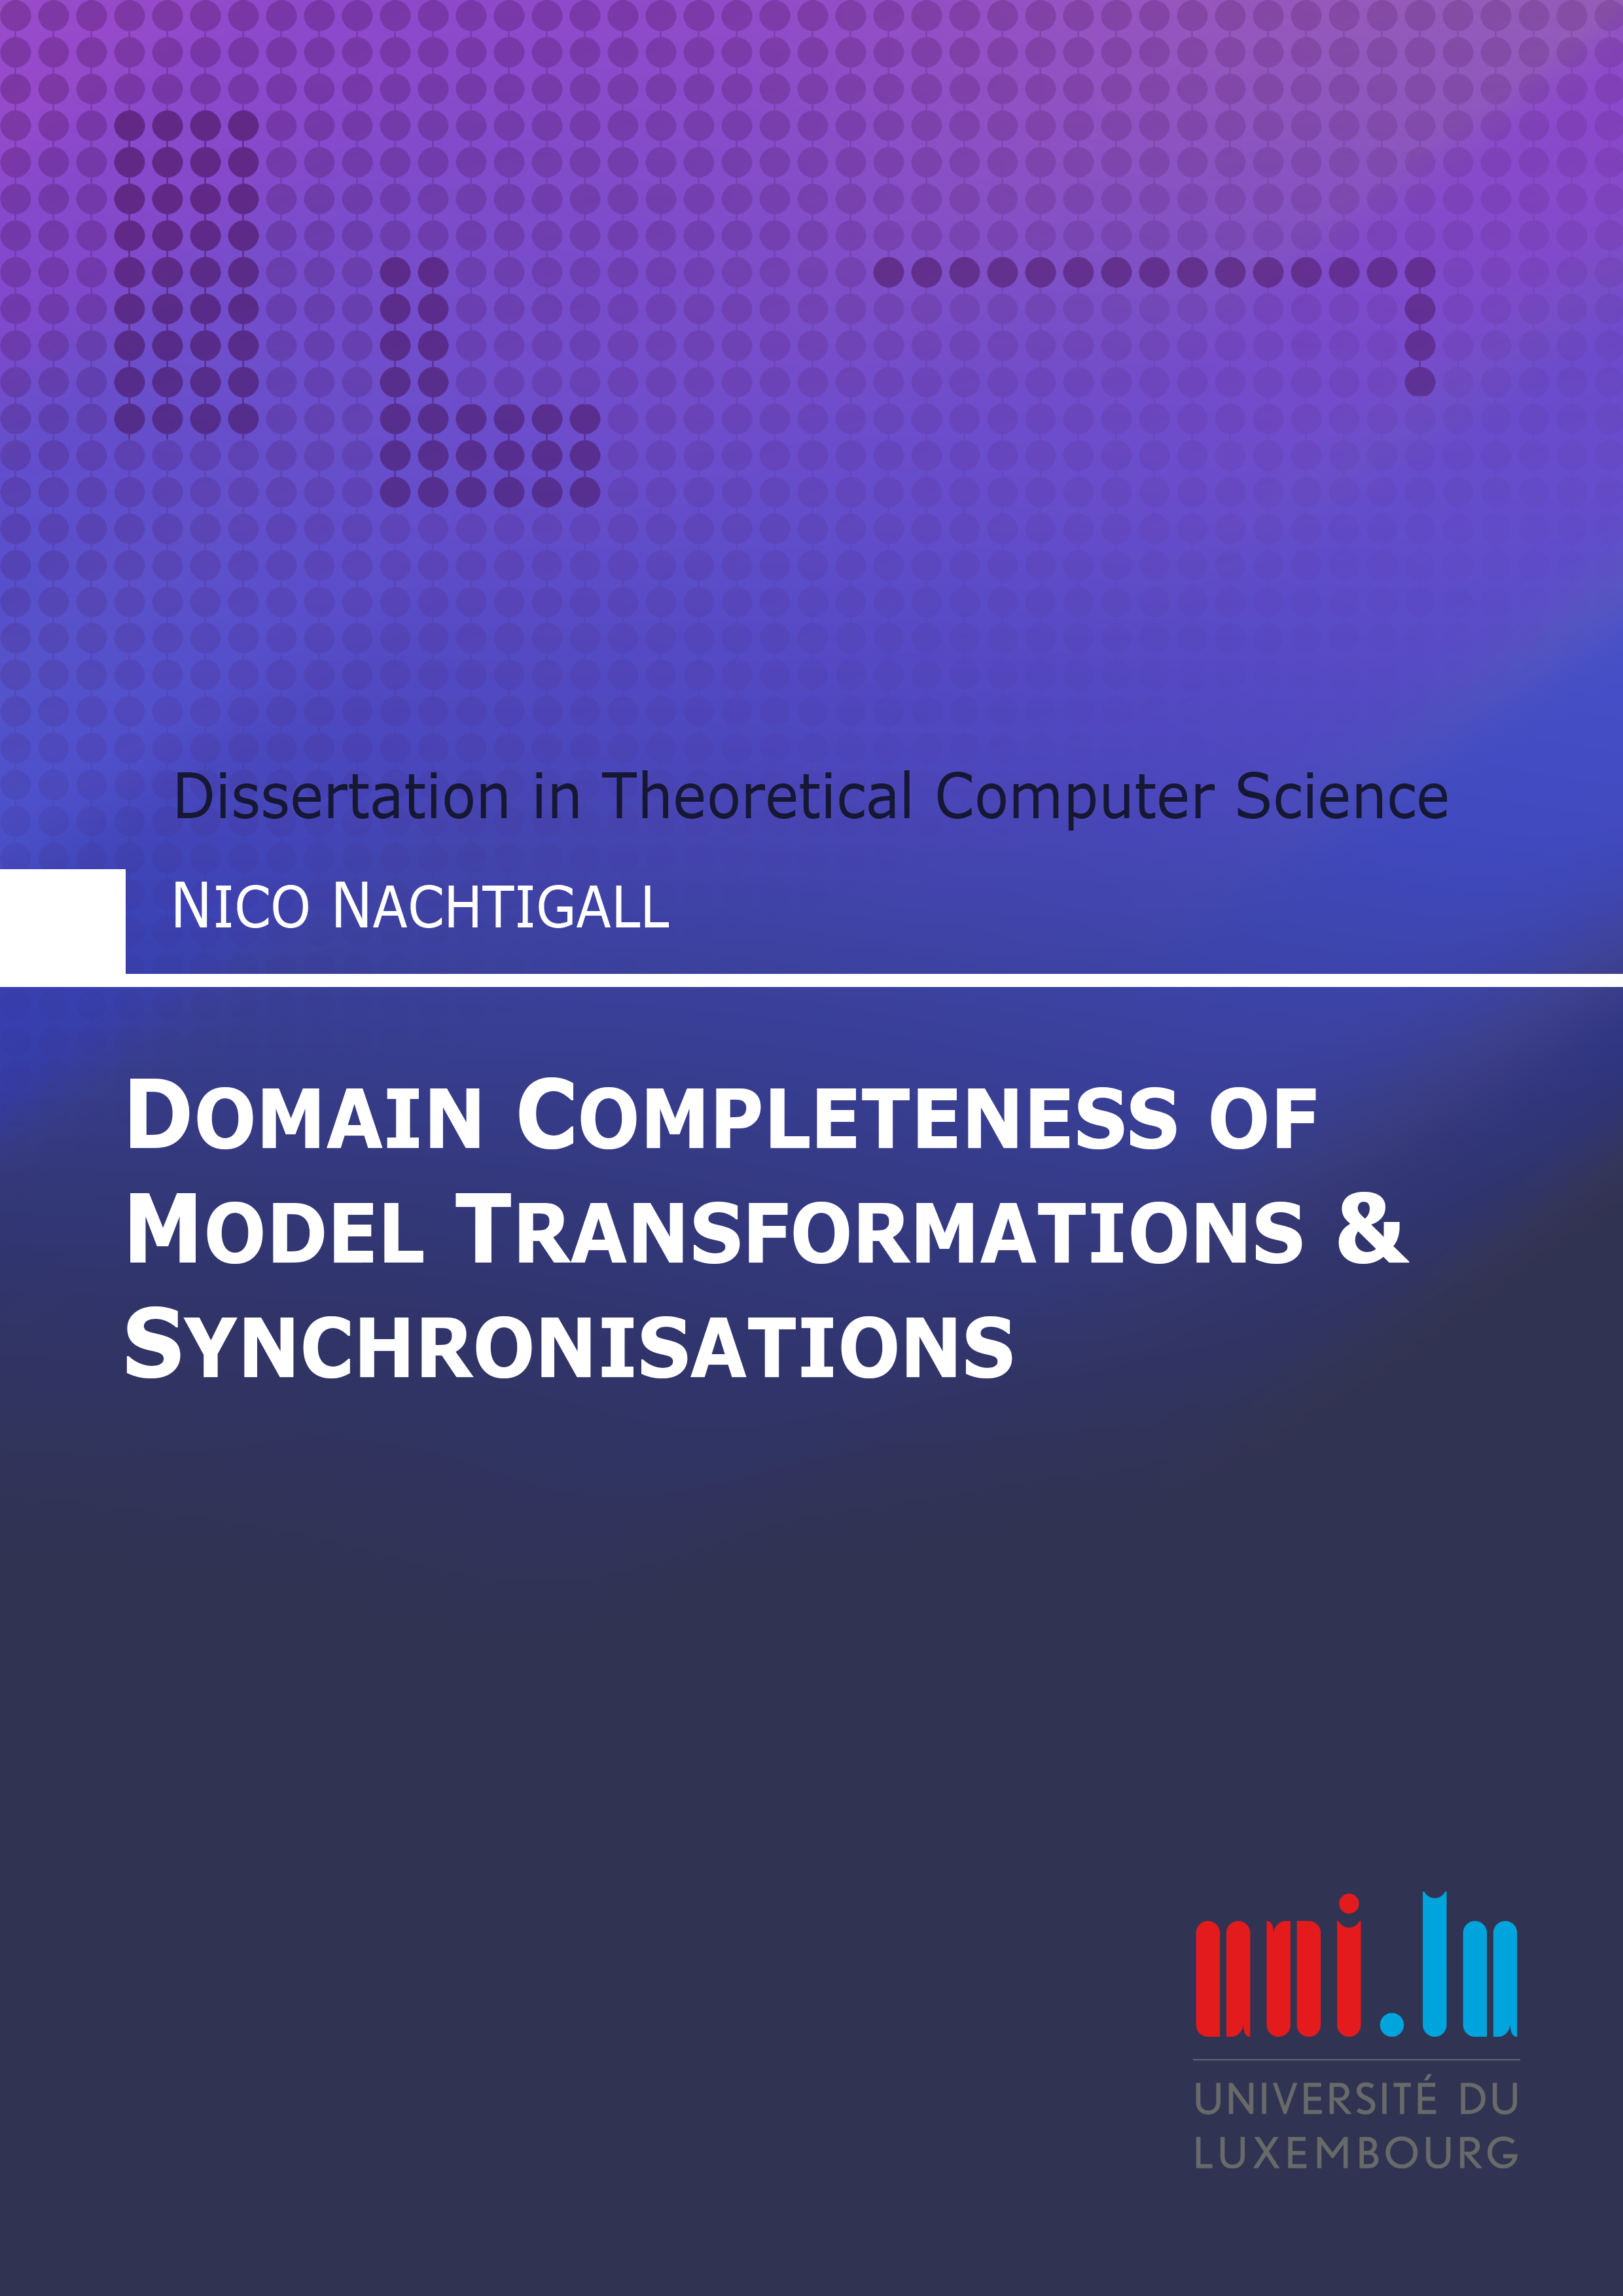
\includepdf[fitpaper,noautoscale=false,offset=-7mm 0mm]{cover/coverfront.png}}

\frontmatter
\thispagestyle{empty}
\begin{minipage}{\textwidth}
    \centering
    \vspace*{-.5cm}
    
\includegraphics[width=0.2\textwidth]{logo.png}\par
    \vspace*{0.5cm}
    PhD-FSTC-2016-33\par
    The Faculty of Sciences, Technology and Communication\par 
    \vspace*{1cm}
    \uppercase{\LARGE{Dissertation}}\par
    \vspace*{.5cm}
    \normalsize{Defense held on 29/08/2016 in Luxembourg}\par
    \normalsize{to obtain the degree of}\par
    \vspace*{.5cm}
    \uppercase{\Large{Docteur de L\'{}universit\'e du Luxembourg en Informatique}}\par
    \vspace*{.5cm}
    \normalsize{by}\par
    \Large{\textsc{Nico Nachtigall}}\par
    \vspace*{.5cm}
    \normalsize{Born on 1st April 1982 in Berlin (Germany)}\par

    \color{headlineColor}
    \LARGE{\textsc{\textbf{\sffamily
    Domain Completeness of Model\\ Transformations and Synchronisations
    }}}\par
    \color{black}

    \vspace*{2cm}
\raggedright{
    \Large{Dissertation defense committee:}\par
    \vspace*{0.5cm}
    \Large{Prof. Dr. Thomas Engel, Dissertation Supervisor}\par
    \normalsize{Professor, Universit\'e du Luxembourg, Luxembourg}\par
    \vspace*{.1cm}
    \Large{Prof. Dr. Barbara K\"onig}\par
    \normalsize{Professor, Universit\"at Duisburg-Essen, Germany}\par
    \vspace*{.1cm}
    \Large{Prof. Dr. Ulrich Sorger, Chairman}\par
    \normalsize{Professor, Universit\'e du Luxembourg, Luxembourg}\par
    \vspace*{.1cm}
    \Large{Dr. Frank Hermann, Deputy Chairman}\par
    \normalsize{Carmeq GmbH, Berlin, Germany}\par
    \vspace*{.1cm}
    \Large{Dr. Raimondas Sasnauskas}\par
    \normalsize{SES Engineering, Luxembourg}\par
    \vspace*{.1cm}
    \Large{Dr. Benjamin Braatz}\par
    \normalsize{Graph-IT GmbH, Cologne, Germany}\par
}

\end{minipage}
\clearpage

\null\newpage

\thispagestyle{plain}
\begin{flushright}
\vspace*{8cm}
\huge
To my sons Emil \& Max, my wife Susann and my grandfather \dag Axel
\end{flushright}
\clearpage
\null\newpage

\addcontentsline{toc}{chapter}{Foreword \& Acknowledgements}
\chapter*{Foreword \& Acknowledgements}
The intrinsic question of most activities in information science, in practice or science, is \textit{``Does a given system satisfy the requirements regarding its application?''}
% Most activities have a link to this question
Commonly, requirements are expressed and accessible by means of models, mostly in a diagrammatic representation by visual models.
% since, requirements not yet realised and exist only via cognitive concepts
The requirements may change over time and are often defined from different perspectives and within different domains.
This implies that models may be transformed either within the same domain-specific visual modelling language or into models in another language.
Furthermore, model updates may be synchronised between different models. %to achieve consistency
Most types of visual models can be represented by graphs where model transformations and synchronisations are performed by graph transformations.
The theory of graph transformations emerged from its origins in the late 1960s and early 1970s as a generalisation of term and tree rewriting systems to an important field in (theoretical) computer science with applications particularly in visual modelling techniques, model transformations, synchronisations and behavioural specifications of models.
Its formal foundations but likewise visual notation enable both precise definitions and proofs of important properties of model transformations and synchronisations from a theoretical point of view and an intuitive approach for specifying transformations and model updates from an engineer's point of view.
The recent results were presented in the EATCS monographs ``Fundamentals of Algebraic Graph Transformation'' (FAGT) in 2006 and its sequel ``Graph and Model Transformation: General Framework and Applications'' (GraMoT) in 2015.
%Visual models important role for visualising cognitive concepts of things obtained by abstractions.
%In computer science, models are models for (sub-)systems.
%Visual notation and the fact that most visual models can be represented by graphs makes graph transformation well-studied underlying concept for specifying dynamic behaviour of models and model transformations.
%Behaviour of automaton and Petri nets.
%In software engeneering, model transformations enforced by MDD, MDA.
%This thesis concentrates on two important properties of model transformations and synchronisations, i.e., syntactical correctness and completeness.
This thesis concentrates on one important property of model transformations and synchronisations, i.e., syntactical completeness.
Syntactical completeness of model transformations means that given a specification for transforming models from a source modelling language into models in a target language, then all source models can be completely transformed into corresponding target models.
In the same given context, syntactical completeness of model synchronisations means that all source model updates can be completely synchronised, resulting in corresponding target model updates.
%On the other hand, syntactical correctness means that the resulting target models actually belong to the target language.
This work is essentially based on the GraMoT book and mainly extends its results for model transformations and synchronisations based on triple graph grammars by a new more general notion of syntactical completeness, namely domain completeness, together with corresponding verification techniques.
Furthermore, the results are instantiated to the verification of the syntactical completeness of software transformations and synchronisations.
%Furthermore, a new concept of complete and correct model transformations (synchronisations) of inconsistent models (model updates) based on triple graph grammars is presented.
The well-known transformation of UML class diagrams into relational database models and the transformation of programs of a small object-oriented programming language into class diagrams serve as running examples.
The existing AGG tool is used to support the verification of the given examples in practice.
%The completeness results may ensure a complete validation of the semantic correctness of model transformations and synchronisations based on semantic checks in the sense that each source model (update) may be tested against the corresponding target model (update).
% \newline
% \newline
This is a revised version of the printed hard copy with additional notes on from domain incompleteness to domain completeness in \cref{sec-dom-compl-mt-synch} and on domain correctness in \cref{sec-conclusion}.

\section*{Acknowledgements}
First of all, I would like to thank Frank Hermann for his great support and patience. He did a great job in
guiding me and answering the big amount of questions that occured during my PhD studies.
Without the help of Frank, this work would not have been possible.
Furthermore, I would like to thank Benjamin Braatz, Barbara K\"onig and Claudia Ermel for
their continous help, for proofreading my work and for answering many questions.
Also many thanks to Thomas Engel and Raimondas Sasnauskas for supervising my thesis and
for giving me the opportunity to finish this thesis.
%\noindent\textbf{Acknowledgements:}
\parpic(0ex,0ex)[r][r]{
\includegraphics[scale=0.38]{img/FNR_logo.jpg}}
\noindent Supported by the Fonds National de la Recherche, Luxembourg 4895603.

\tableofcontents

\mainmatter

\chapter{General Introduction}
\label{sec-gen-intro}

While this chapter gives a short and general introduction to model transformations and synchronisations, its completeness and correctness properties and the main results of this thesis, \cref{sec-mt-ms-ff} gives a more in-depth introduction to model transformations, synchronisations, their properties (in particular the completeness property) and their link to the theory of graph transformations as the underlying formal framework.

\section{Models in Information Science}
\label{sec-gen-intro-models}
Commonly, visual models are considered as being simplified versions of complex systems \cite{Bezivin2005} that are obtained by a process of abstraction either from mental concepts or from the properties and features of the sytem itself if it already exists during model creation.
The process of abstraction requires the identification of important properties of the intended system's application and use while omitting properties and features that are considered as being irrelevant for the intended model usage.
In this context, the properties that are captured by the model are requirements on the intended system's application and use.
In most cases, system models are used in contexts where the system itself is still in the process of being developed, i.e., the system is (requirements are) only accessible by means of models during most stages of development.
Therefore, models have an important role in information science \cite{Fetzer20,Thalheim2011} with an image characteristic in the sense that models are (simplified) images of the originals they represent with the purpose to take models as substitutes for their originals within a given temporal and situational context.
The importance of models in information science is addressed by several communities with the object management group (OMG) being one of the largest global initiatives.
Models are the cornerstones of their work where each complex system is rather being designed by means of visual models before being implemented \cite{Janis01}.
This enables a view on problems and their potential solutions before starting with an (extensive) full implementation and therefore, reduces risks. 
At its extreme, the system is developed strictly by modelling and the implementation is (completely) generated from models, i.e., ``the model is the code.'' \cite{Thalheim2011}.

\begin{figure}[!tb]
\begin{center}
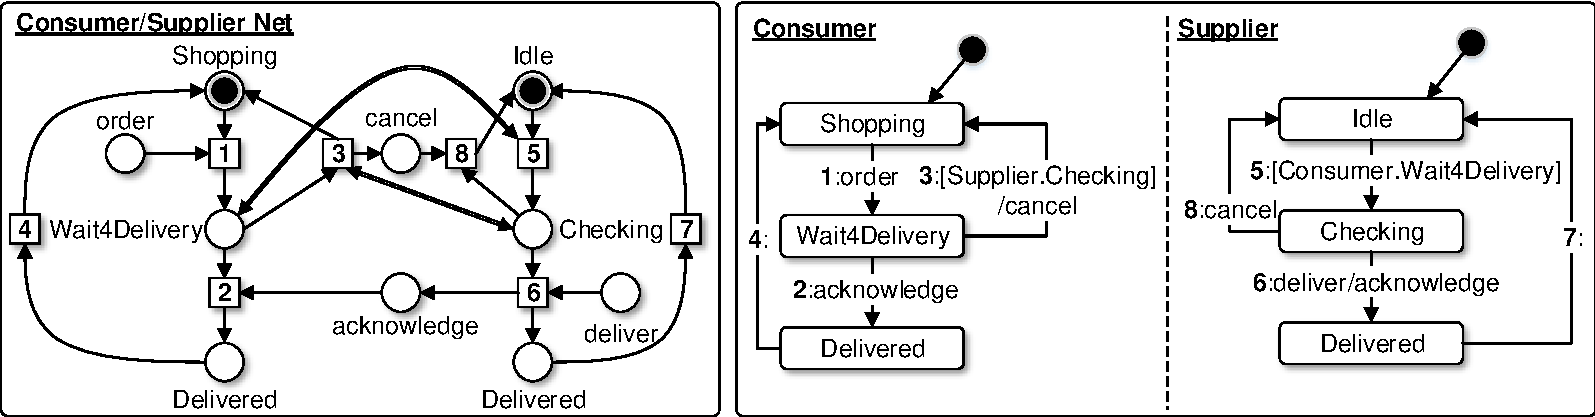
\includegraphics[width=\textwidth]{img/gen_intro/models.pdf}
\end{center}
\caption{Models in Information Science - Place/Transition System (left) \& Statechart (right)}
\label{fig:sec-gen-intro-models:models}
\end{figure}

\begin{figure}[!tb]
\begin{center}
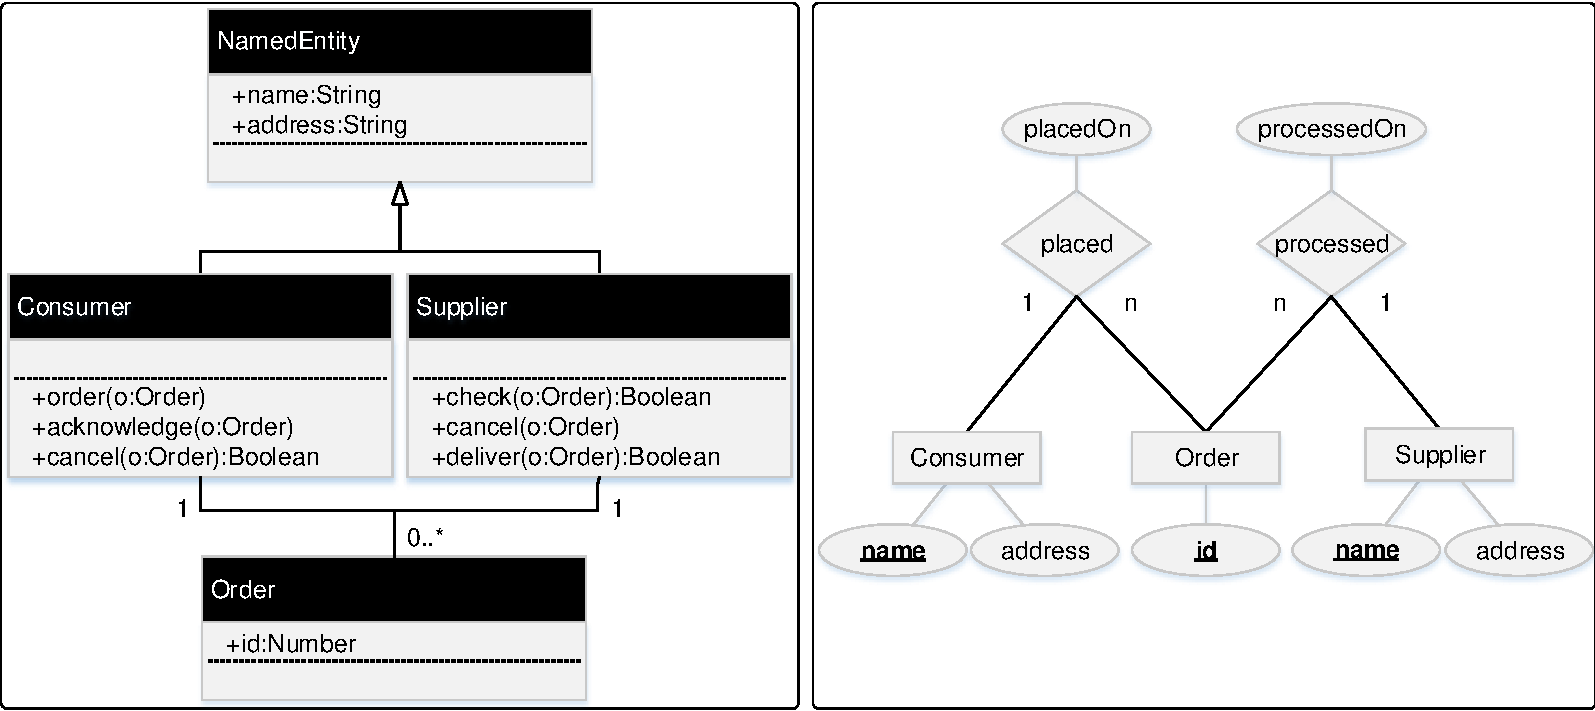
\includegraphics[width=\textwidth]{img/gen_intro/models2.pdf}
\end{center}
\caption{Models in Information Science - UML Class Diagram (left) \& Entity-Relationship Diagram (right)}
\label{fig:sec-gen-intro-models:models2}
\end{figure}

Furthermore it is generally stated that complex systems cannot be comprehended in their entirety, as, the human capacity is limited and therefore, abstractions are necessary that allow us to manage complexity \cite{Quatrani:1998:VMR:275580} by focusing on the relevant details only.
In model-driven software and systems development (MDD), models usually exhibit the following characteristics \cite{Selic:2003:PMD:942589.942714}.
The model must be
{
\renewcommand\labelenumi{(\theenumi)}
\begin{enumerate*}
\item easy to understand for the intended group of model users,
\item accurate, i.e., the model only reflects real properties of the system,
\item predictive, i.e., the model must be a reflection of important, non-obvious properties of a system under development,
\item inexpensive, i.e., the creation and analysis of a model must be cheaper than the implementation of the system and its analysis itself.
\end{enumerate*}
}

Although most models share a common set of properties which make them identifiable as such, Herbert Stachowiak \cite{Stachowiak.1973} and Bernd Mahr \cite{DBLP:journals/sosym/Mahr09,DBLP:journals/eceasst/Mahr10a} each developed a comprehensive theory of model-being.
Instead of identifying an object as a model based on a definition with a fixed set of properties, the model-being of an object is rather the result of a context-specific judgement.
An object $O$ is interpreted as a model $M$ of something $A$ with the purpose for something $B$ and therefore, $O$ carries a cargo (some type of information) from $A$ to $B$.
The model object $O$ is produced based on (a subset of) the properties of original object $A$.
Therefore, these properties must be identifiable in an observation on $O$.
Analogously, purpose $B$ is realised based on (a subset of) the properties of model object $O$.
Therefore, these properties must be identifiable in an observation on the resulting object $B$.
Similarly, \cite{Muller2012} advocates that model-being depends on the existence of a representation relation between model object and its original where a model is considered as the representation of its original.

\cref{fig:sec-gen-intro-models:models,fig:sec-gen-intro-models:models2} depict different types of system models from different perspectives and within different problem domains that are used in MDD \cite{6507223,mdd05,Beydeda2005ModelDriven} for communication between experts of the same domain and across different domains.
\cref{fig:sec-gen-intro-models:models} depicts models of the dynamic behaviour of a given (concurrent) purchase order system that may be used to implement the behaviour in the form of operations in computer programs.
In contrast to \cref{fig:sec-gen-intro-models:models}, \cref{fig:sec-gen-intro-models:models2} depicts models that represent the static organisation of concepts (data) and their interrelationships in the system, i.e., the ontology for the domain of discourse (the purchase order scenario).
These models may be used to implement static aspects of the system, e.g., class definitions in an object-oriented programming language or relational database structures that both may serve as the data basis for the operations in computer programs.

\cref{fig:sec-gen-intro-models:models} (right) illustrates a UML statechart \cite{UML15,Rumbaugh:2004:UML:993859}.
UML statecharts are originated from classical hierarchical Harel statecharts \cite{HAREL1987231,Harel2005} which extend the formalism of finite-state machines \cite{Dathan2015} mostly by hierarchically nested states and orthogonal regions to enhance the readability and scalability of the models.
The statechart consists of (system) states (boxes) and transitions between states (arrows).
Each transition describes some system behaviour by the change from one system state to another state.
Furthermore, the statechart is separated into two orthogonal (concurrently operating) regions as marked by a dashed line.
In each region, the initial state is marked by a black node.
Each transition has an inscription of the form: $[event]['['condition']']['/'action]$ where $[]$ is meant to be optional.
A transition is enabled if the source state of the transition is the current state, the $event$ occured and the $condition$ can be evaluated to true.
If a transition fires, then the current state changes to the target state of the transition and the $action$ is performed.
The following behaviour of a consumer-supplier system is modelled in \cref{fig:sec-gen-intro-models:models} (right):
The consumer and supplier start with \code{Shopping} and \code{Idle}, respectively.
After \code{Shopping}, the consumer may decide to \code{order} and consequently, waits for delivery afterwards (state \code{Wait4Delivery}).
If the consumer is waiting for delivery, the supplier immediately pass over to \code{Checking} the order.
As long as the supplier is \code{Checking} and the consumer is waiting, the consumer may \code{cancel} the order at any time which directly causes a cancellation on the supplier side.
After cancellation both sides return to their initial states.
After \code{Checking}, the supplier may decide to deliver the ordered items while asking the consumer to \code{acknowledge} the receipt at the same time.
Subsequently, the consumer \code{acknowledge}s, both transition into state \code{Delivered} and may return to their initial states at any time.
 
\cref{fig:sec-gen-intro-models:models} (left) depicts a Petri net, more precisely a place/transition net with initial marking \cite{NIELSEN19923,Reisig:1985:PNI:3405}, which captures the same dynamic behaviour from \cref{fig:sec-gen-intro-models:models} (right).
The marking is given by a (black) token distribution which defines the system state.
By firing an enabled transition (boxes) the state can be changed.
A transition is enabled, if each input place (circles with outgoing edges to the corresponding transition) contains a token.
When a transition is fired, all tokens from the input places are removed and for each output place (circles with incoming edges from the corresponding transition) a token is added.
Therefore, for each transition in \cref{fig:sec-gen-intro-models:models} (right) there is a transition defined in \cref{fig:sec-gen-intro-models:models} (left) and the initial states (each state and event) in the statechart are (is) modelled by an initial marking (a place) in the net.

While the statechart delivers a readable model of the behaviour, the Petri net may be used for formal analysis of the behaviour as supported by a variety of existing tools.

\cref{fig:sec-gen-intro-models:models2} (left) presents a UML class diagram \cite{UML15,Rumbaugh:2004:UML:993859}.
The diagram designates classes \code{Consumer}, \code{Supplier} and \code{Order} as central concepts of the system.
\code{Consumer}s and \code{Supplier}s are named entities (cf. inheritance relationship with class \code{NamedEntity}) and therefore, they have a \code{name} and \code{address} both of type \code{String}.
Furthermore, a \code{Consumer} has the following operations (possible behaviour):
A \code{Consumer} may:
\begin{enumerate*}
\item place an \code{Order} \code{o},
\item \code{acknowledge} the receipt of an \code{Order} \code{o}, or
\item \code{cancel} an \code{Order} \code{o} with \code{Boolean} return value. By \cref{fig:sec-gen-intro-models:models}, a cancellation is only possible if the \code{Supplier} is checking the order as indicated by a \code{Boolean} return value which returns \code{true} in case of success and otherwise \code{false}.
\end{enumerate*}
Similarly, a \code{Supplier} may:
\begin{enumerate*}
\item \code{check} an \code{Order} \code{o},
\item \code{cancel} an \code{Order} \code{o}, or
\item \code{deliver} an \code{Order} \code{o}.
\end{enumerate*}
Furthermore by the interrelationships as given in the diagram:
\begin{enumerate*}
\item Each \code{Consumer} may have placed an arbitrary number of \code{Order}s, each \code{Order} identified by an \code{id},
\item each \code{Supplier} may have processed an arbitrary number of \code{Order}s, and
\item each \code{Order} was placed (processed) by exactly one \code{Consumer} (\code{Supplier}).
\end{enumerate*}

\cref{fig:sec-gen-intro-models:models2} (right) presents an entity-relationship diagram containing the same concepts and interrelationships from the class diagram.
However, note that the operations (suggestions of possible behaviour) of the entities are missing, the interrelationships \code{placed} and \code{processed} become explicit figures with additional attributes \code{placedOn} and \code{processedOn} instead of simple arrows and attributes \code{name} and \code{id} are particularly marked as unique instance identifiers (primary keys).

Therefore, the class diagram is rather used to generate the base frame of a program in an object-oriented programming language while the entity-relationship diagram is used to create the structure of a relational database that may be used by the program.

\section{Models, Transformations \& Synchronisations}
\label{sec-gen-intro-trafos}
\cref{sec-gen-intro-models} already highlighted the importance of models in information science especially in the model-driven development of software and systems in general.
It was stated and supported by different concrete examples that models are created and intended to be used in the context of different problem domains where they capture requirements on the intended system's application and use from different perspectives.
The requirements may change over time, need to be refined or may be inferred from requirements that are formulated in other domains.
This implies that models may be transformed either within the same domain-specific modelling language (DSL) or into models in another language.
Furthermore, model updates may be synchronised between interrelated models and different domains.

For example, the net in \cref{fig:sec-gen-intro-models:models} (left) can be completely inferred from the statechart (right).
A corresponding model transformation from models that are formulated in the DSL of UML statecharts into models that are formulated in the DSL of place/transition nets is given in \cite{Ehrig:2006:FAG:1121741}.
Vice versa, UML statecharts cannot be completely inferred from place/transition nets in any cases, since, the statecharts may contain information (e.g., the explicit separation into concurrently operating sub-systems (orthogonal regions)) that are not available in (flat) nets. 
However, a transformation from place/transition nets into statecharts can be used in order to obtain initial statechart models from existing nets and where the statecharts are refined at a later step, e.g., by adding orthogonal regions.
While a transformation from UML statecharts into place/transition nets may be used for simulating the behaviour of the model based on the net \cite{conf/seke/HuS04}, the reverse transformation may be used in order to obtain a more readable model in the form of a statechart from the net.

The same is true for the examples in \cref{fig:sec-gen-intro-models:models2}.
UML class diagrams and entity-relationship diagrams share a common set of knowledge while containing exclusive information at the same time.
While both share the knowledge of domain entitites (\code{Consumer}, \code{Supplier} and \code{Order}) and their interrelationships, class diagrams may additionally capture operations for each entity and entity-relationship diagrams may make the interrelationships more explicit as well as may mark specific attributes as unique instance identifiers (primary keys).
However, analogously to the place/transition net-statechart scenario, it is common practice to derive entity-relationship diagrams from class diagrams and vice versa in order to obtain initial models in the one domain from existing models in the other domain.
This transformation is also referred to as the object-relational mapping between the concepts in object-oriented programming languages and concepts in relational database systems.

By this means, each class diagram may be in relation with a corresponding entity-relationship diagram.
Therefore, a model update on a class diagram need to be synchronised with its entity-relationship diagram and vice versa.
For example, by changing the attribute of entity \code{Order} in \cref{fig:sec-gen-intro-models:models2} (left) from \code{id} to \code{uid}, in order to emphasize the uniqueness of the identifier, this change must lead to a corresponding update in \cref{fig:sec-gen-intro-models:models2} (right).

Note that especially if we think of model-being as a result of a judgement (cf. \cref{sec-gen-intro-models}), ``Everything is a Model'' \cite{Bezivin2005} or more precisely, everything can be construed as a model, be it a mental concept or a physical entity.
In this thesis, we focus on visual models in the form given in \cref{fig:sec-gen-intro-models:models,fig:sec-gen-intro-models:models2}, their transformation and synchronisation.
The typical example of model-to-model transformations, the transformation from UML class diagrams to relational database models (CD2RDBM) \cite{FAGT2}, serves as the running example throughout all chapters.
In \cref{sec-gen-intro-mt-ms}, we review general basic notions of model transformations and synchronisations in more detail.


\section[Graph Transformations for Model Trans. \& Synchronisations]{Graph Transformation for Model Transformations \& Model Synchronisations}
\label{sec-gen-intro-gratrafo}
\begin{figure}[!tb]
\begin{center}
\begin{tikzpicture}[]
\fill (0,0) node[inner sep=1pt] (A) {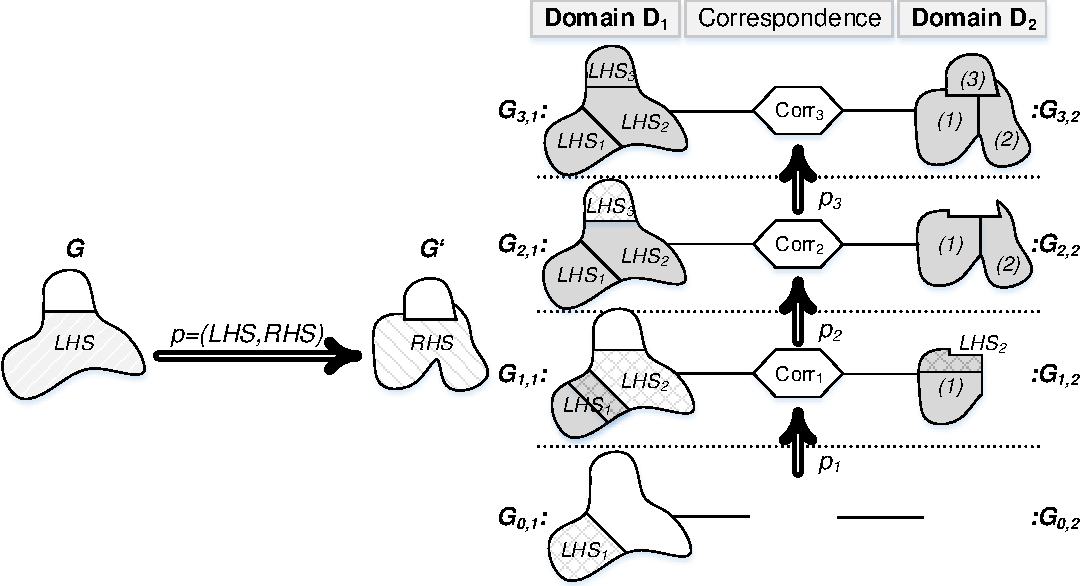
\includegraphics[width=\textwidth]{img/gen_intro/gts.pdf}};
\fill (3.55,-3.1) node[inner sep=1pt] (B) {\huge{$\varnothing$}};
\fill (5.9,-3.1) node[inner sep=1pt] (C) {\huge{$\varnothing$}};
\end{tikzpicture}
\end{center}
\caption{Rule-Based Graph Transformation Step (left) \& Model Transformation Sequence (right)}
\label{fig:sec-gen-intro-gratrafos:trafos}
\end{figure}

In this thesis, the theory of graph transformations is used as the consistent formal framework for defining models, model updates and model transformations as well as for performing model transformations and synchronisations \cite{Ehrig:2006:FAG:1121741,FAGT2}.
Therefore, models are represented by graphs.
We assume that most types of visual models as given in \cref{sec-gen-intro-models} can be represented by graphs.
Essentially, a graph consists of a set of nodes and a set of edges between nodes.
A model update defines which part of a graph is deleted and which part is added by the update.
A model transformation is defined in terms of a set of graph transformation rules.
A transformation rule (or production) $p=(\LHS,\RHS)$ contains a left-hand side (LHS) and a right-hand side (RHS).
When applying a rule $p$ to a graph $G$, then $G$ is transformed in the sense that LHS is replaced by RHS in $G$ leading to a new graph $G'$, denoted by $G \Trans{p} G'$ (cf. \cref{fig:sec-gen-intro-gratrafos:trafos} (left)).
Therefore, if $\LHS$ is a subgraph of $\RHS$ (i.e., $p$ only creates elements and therefore is non-deleting) then $\RHS \setminus \LHS$ is mainly added to $G$ while $\LHS$ is preserved by the rule application.
Otherwise, if intersection $\LHS \cap \RHS \neq \LHS$, then $\LHS \setminus \RHS$ is deleted in $G$, $\LHS \cap \RHS$ is preserved and $\RHS \setminus \LHS$ is added to $G$.
Note that this is an intuitive approach to graph transformations via set-theoretic operations $\setminus$ and $\cap$ on nodes and edges of graphs while technically, transformations are defined based on the category-theoretic concept of pushouts (cf. \cref{sec-gt-trafo}).

Commonly, model transformations from models in source domain $D_1$ (e.g., UML class diagrams) into models in target domain $D_2$ (e.g., entity-relationship diagrams) are defined based on a set of non-deleting graph transformation rules and performed by graph transformations, i.e., by applying transformation rules successively (so called model transformation sequences) as illustrated in \cref{fig:sec-gen-intro-gratrafos:trafos} (right).
The source (input) model (graph) $G_{0,1}$ of a transformation sequence in source domain $D_1$ is traversed step-wise in $n$ steps and target (output) model (graph) $G_{n,2}$ in target domain $D_2$ is constructed in parallel as follows:
\begin{enumerate}
\item At each step $i$ ($i \in \{1\ldots n\}$), a rule $p_i=(\LHS_i,\RHS_i)$ is applied to graph $(G_{i-1,1} \gets Corr_{i-1} \to G_{i-1,2})$ leading to a new graph $(G_{i,1} \gets Corr_{i} \to G_{i,2})$ where $G_{i,1}$ represents the graph part in domain $D_1$, $G_{i,2}$ the graph part in domain $D_2$ and $Corr_i$ is the correspondence that relates elements from $G_{i,1}$ with elements from $G_{i,2}$. - The model transformation sequence in \cref{fig:sec-gen-intro-gratrafos:trafos} (right) consists of three steps ($n=3$).
\item At the first step, only source graph $G_{0,1}$ is given as input to the transformation while $Corr_0$ and $G_{0,2}$ are empty (- nothing is transformed yet).
Therefore, by applying rule $p_1$, $\LHS_1$ in $G_{0,1}$ is marked as transformed in $G_{1,1}$ (by dark grey colouring) and $Corr_1$ with dark grey area $(1)$ are added (i.e., $\LHS_1$ in $G_{0,1}$ is transformed into $G_{1,2}=(1)$).
\item Analogously, in the following steps $i$, $\LHS_i$ in $(G_{i-1,1} \gets Corr_{i-1} \to G_{i-1,2})$ is transformed into $(i)$ in $G_{i,2}$.
Note that $\LHS_i$ may overlap with already transformed elements.
For example in Step 2 in \cref{fig:sec-gen-intro-gratrafos:trafos} (right), $\LHS_2$ overlaps with $\LHS_1$ in domain $D_1$ and with $(1)$ in domain $D_2$ and the result of Step 2 is that $\LHS_1 + \LHS_2$ in $D_1$ together are transformed into $(1)+(2)$ in $D_2$.
Step 3 in \cref{fig:sec-gen-intro-gratrafos:trafos} (right) shows the case where $\LHS_i$ in $D_1$ is transformed one-to-one without changing its structure into $(i)$ in $D_2$.
This is especially true for model refactorings where domains $D_1=D_2$, most steps are identical transformations and only a small part of the input graph is changed and therefore transformed into different structures.
\item The transformation sequence terminates and is complete, if the input graph $G_{0,1}$ is completely transformed, i.e., if $G_{0,1}$ is completely coloured (or marked) with dark grey such as is the case after Step 3 in \cref{fig:sec-gen-intro-gratrafos:trafos} (right).
\end{enumerate}
Thus, the rules for the model transformation are non-deleting, since, the source model is not transformed in-place but is only traversed step-wise and is rather preserved by the transformation while the target model is constructed in parallel.

Model synchronisations are performed based on model transformations w.r.t. a given model update.

In the literature, a variety of different graph transformation approaches is discussed with each having its own replacement mechanism for $\LHS$ by $\RHS$ in rule applications \cite{Rozenberg:1997:HGG:278918,Ehrig:1999:HGG:328523,graphgrammarhandbook99}. 
In this thesis, we use the algebraic approach to graph transformations \cite{Ehrig:2006:FAG:1121741} which was extended to model transformations and synchronisations in \cite{FAGT2}.
In \cref{sec-gen-intro-gt}, we review basic notions of algebraic graph transformation.
In \cref{sec-gen-intro-mt-ms-tgg}, we review basic technical notions and concepts of model transformations and synchronisations based on graph transformations.

\section{Organisation of this Thesis \& Main Results}
\begin{figure}[!tb]
\begin{center}
\begin{tikzpicture}[]
\fill (0,0) node[inner sep=1pt] (A) {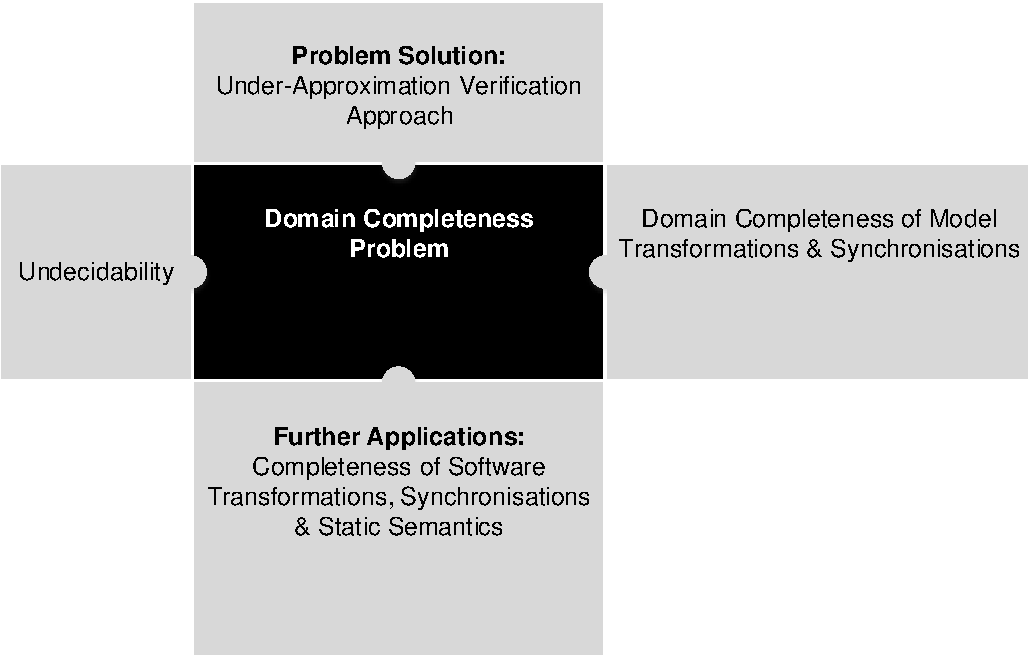
\includegraphics[width=.9\textwidth]{img/gen_intro/bigpicture.pdf}};
\fill (-1.5,.1) node[inner sep=1pt] (B) {\Large{\textcolor{white}{$\Lang(C) \subseteq \Lang(\GG)$?}}};
\fill (3.85,.1) node[inner sep=1pt] (C) {\Large{$\Lang(C) \subseteq \Lang(\TGG)^S$}};
\fill (-1.45,-3.4) node[inner sep=1pt] (D) {\Large{$\Lang(\EBNF) \equiv \Lang(C)$}};
\end{tikzpicture}
\end{center}
\caption{Main Results of this Thesis}
\label{fig:sec-gen-intro-org:bp}
\end{figure}

\cref{fig:sec-gen-intro-org:bp} presents the main results of this thesis.
The domain completeness problem is introduced as the core problem statement.
Generally, we assume that the set of allowed models (graphs) in a given domain of discourse $D$, i.e., the visual domain-specific modelling language (DSL) of $D$, is defined by a set of (domain) graph constraints.
A graph constraint formulates structural restrictions on graphs.
Given a set of constraints $C$, then $\Lang(C)$ is the set of all graphs that satisfy the restrictions which are formulated by the domain constraints in $C$.
Therefore, $\Lang(C)$ is the set of allowed models (graphs) in the given domain $D$, i.e., $\Lang(C)$ is the DSL of $D$.
On the other hand, a set of graph transformation rules together with a start graph form a graph grammar $\GG$.
With $\Lang(\GG)$ we denote the language of graphs that can be created by rule applications starting at the start graph.
The domain completeness problem is defined as follows: Does it hold that $\Lang(C) \subseteq \Lang(\GG)$?
Therefore, can all graphs that satisfy the domain constraints in $C$ be created from the start graph in $\GG$ by successively applying the rules of graph grammar $\GG$? - OR - Is the set of domain constraints $C$ as restrictive as or more restrictive than grammar $\GG$, respectively? - OR - Is DSL $\Lang(C)$ completely covered by the graph grammar $\GG$?

It turns out that the domain completeness problem is undecidable in general, i.e., we cannot find a complete computable solution to this problem.
Therefore, we propose an under-approximation solution to the domain completeness problem in order to verify the language inclusion $\Lang(C) \subseteq \Lang(\GG)$ of domain completeness approximately.
Basically, the solution consists of a set of conditions that are sufficient but not necessary and need to be verified.
Therefore, the solution may lead to false negatives but not to false positives, i.e., if the conditions are fulfilled, then it is ensured that the language inclusion holds. 
If the conditions are not fulfilled, then the language inclusion may hold or not hold and additional checks may be necessary in order to obtain (partial) truth.

Furthermore, we developed three main applications of the solution (cf. \cref{fig:sec-gen-intro-org:bp}).
%Initially, we stated the domain completeness problem in view of model transformations and generalised the problem to general graph grammars afterwards.
The domain completeness problem of model transformations is stated as follows: Can all allowed models in the given domain $D$ (all graphs in $\Lang(C)$) be transformed based on a given triple graph grammar $\TGG$? - OR - Does it hold that $\Lang(C) \subseteq \Lang(\TGG)^S$ for forward model transformations or $\Lang(C) \subseteq \Lang(\TGG)^T$ for backward model transformations?
%In order to return to the initial idea, 
Therefore, we have instantiated our solution to the approximate verification of the language inclusion $\Lang(C) \subseteq \Lang(\TGG)^S$ or $\Lang(C) \subseteq \Lang(\TGG)^T$, respectively.
Thus, the language inclusion problem is stated in the context of a triple graph grammar $\TGG$ \cite{DBLP:journals/eceasst/AnjorinLS15,DBLP:conf/gg/SchurrK08,DBLP:conf/wg/Schurr94} instead of a flat graph grammar $\GG$ where the $\TGG$ specifies the model transformation.
The domain completeness problem of model synchronisations is stated analogously: Can all allowed model updates in the given domain be synchronised?
We show that this problem can be verified based on the results of model transformations.
% According to \cref{sec-sem-cor}, the completeness results may ensure a complete validation of the semantic correctness of model transformations and synchronisations based on semantic checks.
The third application of the solution is to verify the completeness of software transformations and synchronisations: 
\begin{enumerate}
  \item Can all programs (their abstract syntax trees (ASTs)) written in a given programming language be transformed? 
  \item Can all program updates (updates of their abstract syntax trees (ASTs)) be synchronised?
\end{enumerate}
Programs written in a given programming language are represented by their abstract syntax models (ASTs) and transformed by performing model transformations of ASTs based on a given $\TGG$.
Commonly, programming languages are defined by a context-free word grammar.
Therefore the third application of the solution mainly focuses on %the 
solving the % Kommentar Frank
problem to close the gap between the word grammar world and graph world by presenting a mapping from a context-free grammar in Extended-Backus-Naur Form (EBNF) notation into a set of graph constaints $C$ such that the language of ASTs over the EBNF $\Lang(\EBNF)$ is equivalent (isomorphic) to $\Lang(C)$, i.e., $\Lang(\EBNF) \equiv \Lang(C)$.

\cref{fig:sec-gen-intro-org:publications} presents the peer-reviewed publications for the period of this thesis and their assignment to the corresponding chapters.
Publications that are not assigned to a chapter contain no direct contribution to this thesis.

\begin{figure}[!tb]
\begin{center}
\begin{tabular}{| p{6.5cm} | p{5.5cm} | c |}
  \hline			
  \textbf{Title} & \textbf{Authors} & \textbf{Chapter} \\
  \hline
  Towards the Propagation of Model Updates along different Views in Multi-View Models \cite{DBLP:conf/etaps/GottmannNE0E16} &
  Susann Gottmann, Nico Nachtigall, Claudia Ermel, Frank Hermann, Thomas Engel & 
  - \\
  \hline
  Triple Graph Grammars in the Large for Translating Satellite Procedures \cite{DBLP:conf/icmt/0001GNEBMPEE14} & 
  Frank Hermann, Susann Gottmann, Nico Nachtigall, Hartmut Ehrig, Benjamin Braatz, Gianluigi Morelli, Alain Pierre, Thomas Engel, Claudia Ermel & 
  \cref{sec-compl-software-trans} \\
  \hline
  Solving the FIXML2Code-case Study with HenshinTGG \cite{DBLP:conf/staf/0001NBEG14} & 
  Frank Hermann, Nico Nachtigall, Benjamin Braatz, Thomas Engel, Susann Gottmann & 
  - \\
  \hline
  Towards Domain Completeness for Model Transformations Based on Triple Graph Grammars \cite{DBLP:conf/staf/Nachtigall0BE14} & 
  Nico Nachtigall, Frank Hermann, Benjamin Braatz, Thomas Engel & 
  \cref{sec-dom-compl} \\
  \hline
  On an Automated Translation of Satellite Procedures Using Triple Graph Grammars \cite{DBLP:conf/icmt/HermannGNBMPE13} & 
  Frank Hermann, Susann Gottmann, Nico Nachtigall, Benjamin Braatz, Gianluigi Morelli, Alain Pierre, Thomas Engel & 
  \cref{sec-compl-software-trans} \\
  \hline
  Correctness and Completeness of Generalised Concurrent Model Synchronisation Based on Triple Graph Grammars \cite{DBLP:conf/models/Gottmann0NBEEE13} & 
  Susann Gottmann, Frank Hermann, Nico Nachtigall, Benjamin Braatz, Claudia Ermel, Hartmut Ehrig, Thomas Engel & 
  \cref{sec-dom-compl-synch} \\
  \hline
  Symbolic Execution of Satellite Control Procedures in Graph-Transformation-Based {EMF} Ecosystems \cite{DBLP:conf/models/NachtigallBE13} & 
  Nico Nachtigall, Benjamin Braatz, Thomas Engel & 
  \cref{sec-compl-oper-sem} \\
  \hline			
  Transformation Systems with Incremental Negative Application Conditions \cite{DBLP:conf/wadt/CorradiniHHGN12} & 
  Andrea Corradini, Reiko Heckel, Frank Hermann, Susann Gottmann, Nico Nachtigall & 
  - \\
  \hline  
\end{tabular}
\end{center}
\caption{List of Publications}
\label{fig:sec-gen-intro-org:publications}
\end{figure}

After we have introduced the main results, we refer briefly to their chapters.

\subsection{Chapter 2: Model Transformations, Model Synchronisations \& Formal Framework}
While \cref{sec-gen-intro} gives a general introduction to the topic, in \cref{sec-mt-ms-ff}, we give a more in-depth introduction to model transformations and synchronisations.
We recall different classes of transformations and synchronisations, i.e.:
\begin{enumerate}
  \item In-place transformations vs. ``external" transformations that preserve the source models,
  \item horizontal vs. vertical transformations,
  \item endogeneous vs. exogeneous transformations, and
  \item model (text)-to-model (text) transformations.
\end{enumerate}  
Moreover, we clarify how meta-modelling is linked to model transformations and synchronisations.

We recall basic definitions and results of the theory of algebraic graph transformation.
In particular this includes the category $\AGraphs_\ATGI$ of typed attributed graphs with node type inheritance, their rule-based transformation, graph grammars, (nested) graph conditions and constraints and $\M$-adhesive transformation systems that generalise the concepts from attributed graphs to a variety of different types of graphs (and other structures).
Note that the main results have been developed with a focus to be applied in $\AGraphs_\ATGI$.
Furthermore, we review the notions of triple graphs, triple graph grammars (TGGs) and model transformations / synchronisations based on TGGs.
Finally, we give an overview of important properties of model transformations and synchronisations with a focus to the completeness property.

\subsection{Chapter 3: Domain Completeness}
\cref{sec-dom-compl} introduces the domain completenes problem, shows its undecidability and presents an approximative solution to this problem.
It is shown how to verify the domain completeness problem.
Moreover, limitations of the verification approach are discussed and the concept of recursive graph constraints is introduced in order to allow an application of the approach in the context of infinite domain constraints.
For example, infinite graph constraints are used when describing regular paths in graphs. 
Two methods are presented for deriving finite graph constraints from infinite graph constraints such that the verification process can terminate.
Finally, we consider the verification of domain completeness under restrictions of the domain type graph.
This reflects the situation where only a subset of all constituents of the given domain is subjected to the verification.

\subsection{Chapter 4: Domain Completeness of Model Transformations \& Model Synchronisations}
In \cref{sec-dom-compl-mt-synch}, we instantiate the results from \cref{sec-dom-compl} to the verification of domain completeness of model transformations and model synchronisations.
We reformulate the completeness problem in the context of transformations and distinguish between forward and backward domain completeness of transformations and synchronisations.

\subsection{Chapter 5: Further Applications}
\cref{sec-further-appl} presents further applications of the previous verification results for domain completeness.
In particular, this includes the instantiation of the results to the verification of the completeness of software transformations and synchronisations.
Furthermore, it is shown to which extend the concept of recursive graph constraints from \cref{sec-dom-compl} can be used for the verification of completeness in the context of expressing static semantics in models.

\subsection{Chapter 6: Conclusion, Related \& Future Work}
In \cref{sec-conclusion} we conclude and discuss related work and aspects of future work.

\chapter[Model Transformations, Synchronisations \& Framework]{Model Transformations, Model Synchronisations \& Formal Framework}
\label{sec-mt-ms-ff}

\section{General Introduction to Model Transformations \& Synchronisations}
\label{sec-gen-intro-mt-ms}

The initial introduction to model transformations and synchronisations from \cref{sec-gen-intro-trafos} is extended to a more detailed view in the following \cref{sec-gen-intro-mt,sec-gen-intro-msynch}.

\subsection{Model Transformation}
\label{sec-gen-intro-mt}
\cref{fig:sec-gen-intro-mt:mt} illustrates different types of model transformations.
In general, a model transformation $\MT\colon \Lang(D_1) \TransMT \Lang(D_2)$ is a relation that maps (transforms) models $M \in \Lang(D_1)$ in a domain-specific modelling language (DSL) $\Lang(D_1)$ in source domain $D_1$ (in)to models $M' \in \Lang(D_2)$ in DSL $\Lang(D_2)$ in target domain $D_2$ \cite{Mens2006125}.
Therefore, $(M,M') \in \MT$ means that model $M$ expressed in modelling language $\Lang(D_1)$ is transformed into model $M'$ expressed in modelling language $\Lang(D_2)$ via model transformation $\MT$.
The model transformation is exogeneous if lanuage $\Lang(D_1)$ differs from langauge $\Lang(D_2)$ ($\Lang(D_1) \neq \Lang(D_2)$) and is endogeneous otherwise ($\Lang(D_1)=\Lang(D_2)$).
Moreover, the model transformation is horizontal if the models in $\Lang(D_1)$ and the models in $\Lang(D_2)$ are representations of their originals at the same layer of abstraction.
Otherwise, if the layer of abstraction of $\Lang(D_1)$ differs from the layer of abstraction of $\Lang(D_2)$, then the model transformation is vertical.
According to \cite{Mens2006125}, the following examples highlight the different types of transformations:
\begin{enumerate}
  \item \textbf{Endogenous \& horizontal:} Model refactoring or simplification, i.e., changing or simplifying the internal structure of a model in order to obtain a better readability, reusability, modularity or adaptability but without changing the meaning or behaviour of the model itself,
  \item \textbf{Endogenous \& vertical:} Model refinement (abstraction), e.g., by addding (removing) more concrete (platform-specific) details to (from) a model while staying in the same modelling language,
  \item \textbf{Exogenous \& horizontal:} Language migration, i.e., migration of models from one DSL to another modelling language but by staying at the same layer of abstraction, and
  \item \textbf{Exogenous \& vertical:} Code (model) generation, i.e., transforming visual models expressed in a more abstract (platform-independent) DSL into abstract syntax trees over a platform-specific programming language that are serialised to source code at a later step (or vice versa), e.g., the transformation from UML class diagrams into Java source code \cite{Czarnecki:2006:FSM:1165093.1165106}.
\end{enumerate}

For example, the model transformations from UML statecharts into place/transition nets and from UML class diagrams into entity-relationship diagrams or vice versa in \cref{sec-gen-intro-trafos} are exogenous transformations.
If we neglect details that are only prevailing in one domain, e.g., orthogonal regions in statecharts or operations in class diagrams, then these transformations may be considered as horizontal.
Otherwise, they are rather vertical transformations, e.g., the additional knowledge of operations of classes in class diagrams together with their visibilities to system developers (+ for public, - for private etc., cf. \cref{fig:sec-gen-intro-models:models2}) gives a more concrete and platform-specific view on the system compared to entity-relationship diagrams in this aspect.
Transforming class diagrams by adding operations to classes in the diagrams is rather a model refinement, i.e., an endogenous and vertical model transformation.
In contrast, a simple renaming of class or attribute names is an endogenous and horizontal transformation.
In the literature, endogenous model transformations are associated with model rephrasing and exogenous transformations are associated with model translations.

\begin{figure}[!tb]
\begin{center}
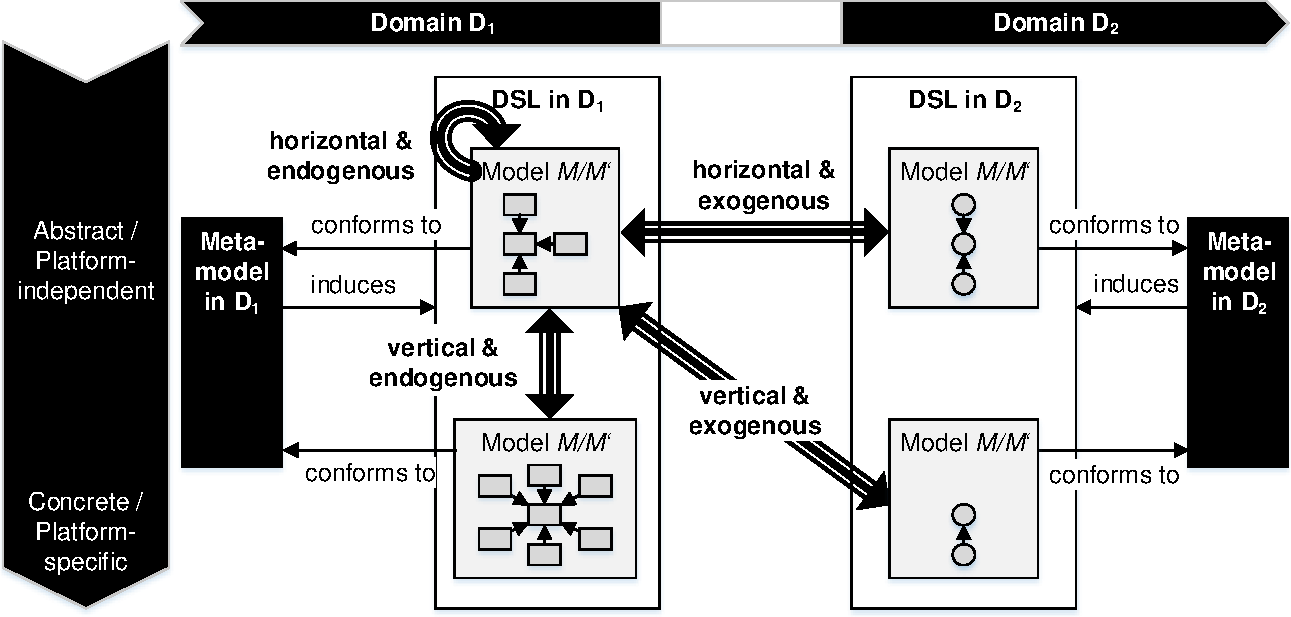
\includegraphics[width=\textwidth]{img/gen_intro/mt.pdf}
\end{center}
\caption{Classification of Model Transformations (Adaption from \cite{FAGT2})}
\label{fig:sec-gen-intro-mt:mt}
\end{figure}

\begin{figure}[!tb]
\begin{center}
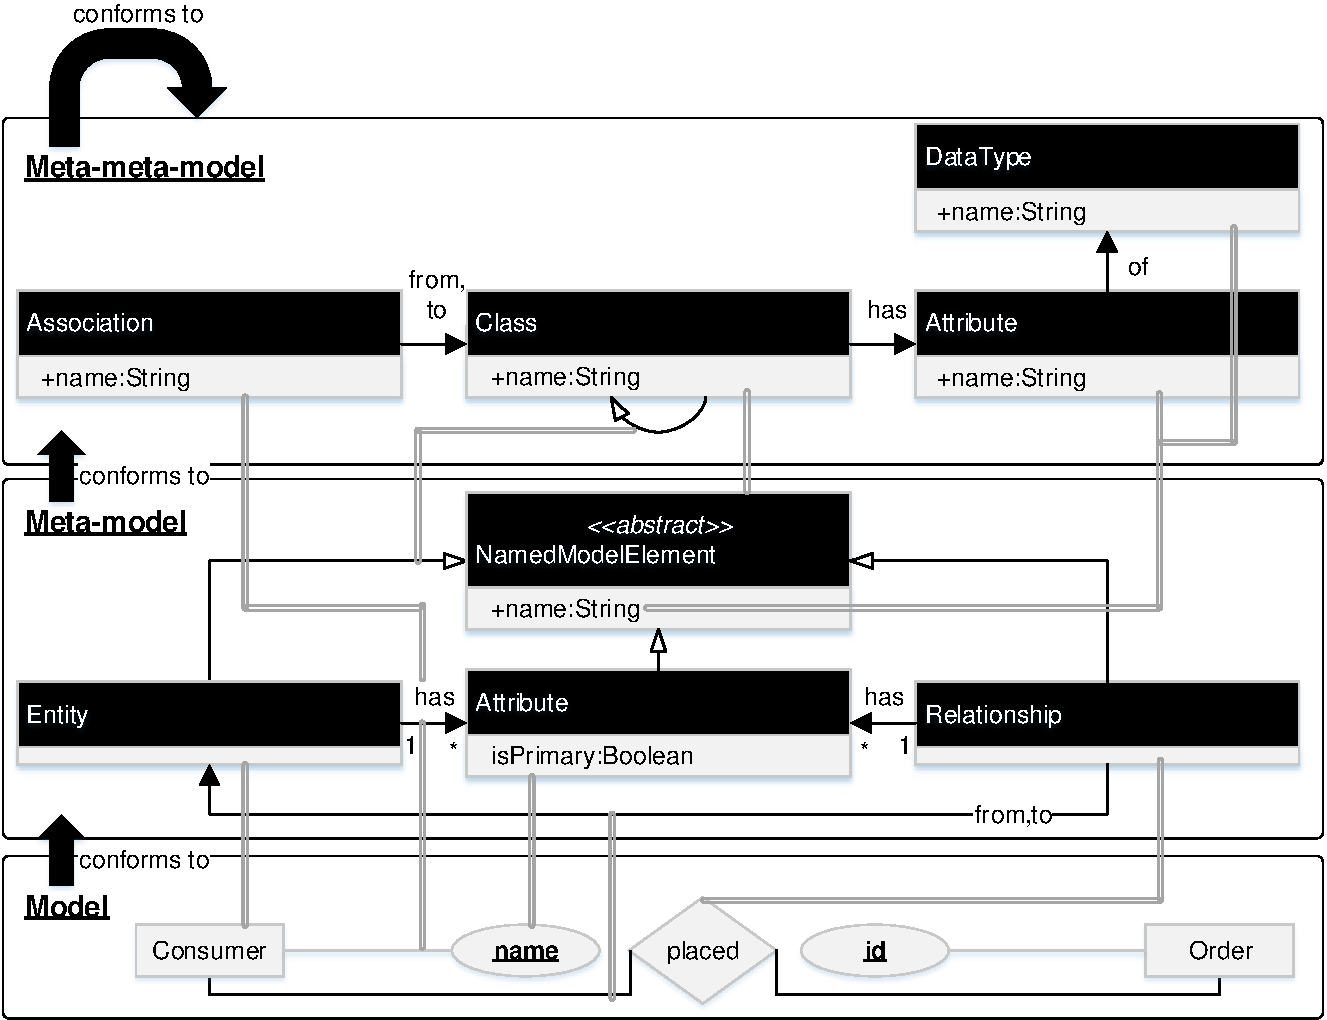
\includegraphics[width=.95\textwidth]{img/gen_intro/meta.pdf}
\end{center}
\caption{Different Layers of Meta-Modelling}
\label{fig:sec-gen-intro-mt:meta}
\end{figure}

Furthermore, DSLs $\Lang(D_1)$ and $\Lang(D_2)$ are each defined by a meta-model in the corresponding domain, i.e., $\Lang(D_1)$ ($\Lang(D_2)$) is induced by a meta-model in domain $D_1$ ($D_2$) (cf. \cref{fig:sec-gen-intro-mt:mt}).
The meta-model defines the concepts of the domain and their interrelationships that can be used in models.
In turn, $\Lang(D_1)$ ($\Lang(D_2)$) is the set of all models that conform to the meta-model in $D_1$ ($D_2$), i.e., the models only contain the concepts and interrelationships of the meta-model as model elements.
For example, we consider the DSL of entity-relationship diagrams in the domain where we want to reflect over the different entities of a system and their interrelationships.
The modelling language is defined by the meta-model in \cref{fig:sec-gen-intro-mt:meta}.
Entity-relationship diagrams may contain several \code{Entit}ies and directed \code{Relationship}s between them, i.e., each relationship is directed \code{from} an entity \code{to} an entity.  
Moreover, entities and relationships may have several \code{Attribute}s that may be primary keys (\code{isPrimary}).
By inheritance, each entity, relationship and attribute is a \code{NamedModelElement} and therefore, has a \code{name} of type \code{String}.
Note that the class \code{NamedModelElement} is declared as \code{<<abstract>>}, i.e., entity-relationship diagrams are not allowed to directly contain nodes of type \code{NamedModelElement} but only in the form of entities, relationships and attributes.
Therefore, the language of entity-relationship diagrams is given by all diagrams (models) that conform to the meta-model.
For example, the model in \cref{fig:sec-gen-intro-mt:meta} conforms to the meta-model.
\code{Consumer} and \code{Order} are \code{Entit}ies whereas \code{placed} is a \code{Relationship} \code{from} \code{Consumer} \code{to} \code{Order}.
Entity \code{Consumer} (\code{Order}) \code{has} a \code{name} (\code{id}) as \code{Attribute} which is marked as primary key (\code{isPrimary}=$\true$).

This view can also be applied to the meta-model where the language of meta-models is defined by a meta-meta-model.
Most meta-models can be expressed by means of the concepts of class diagrams that are given in excerpts by the meta-meta-model in \cref{fig:sec-gen-intro-mt:meta}.
Each meta-model may contain several \code{Class}es and \code{Association}s \code{from} classes \code{to} classes.
Furthermore, each class may have several \code{Attributes} \code{of} some \code{DataType} and with some \code{name} of type \code{String}.
Between two classes there may be an inheritance relationship.
For example, the meta-model in \cref{fig:sec-gen-intro-mt:meta} conforms to the meta-meta-model.
\code{Entity}, \code{Attribute} and \code{Relationship} are \code{Class}es that inherit from class \code{NamedModelElement}.
From class \code{Entity} to class \code{Attribute} there is an \code{Association} with \code{name} \code{has}.
The same is true for class \code{Relationship} and \code{Attribute}.
The class \code{Attribute} \code{has} an \code{Attribute} with \code{name} \code{isPrimary} \code{of} \code{DataType} \code{Boolean}.
Analogously, class \code{NamedModelElement} has an attribute of name \code{name} and of type \code{String}.
In turn, the language of meta-meta-models can be defined by a meta$^3$-model such that the meta-meta-models conform to the meta$^3$-model etc..
However, in order to have a closure over the ``conforms to'' relation, OMG proposes a three-layer hierarchy of meta-modelling, i.e., models, meta-models and meta-meta model, where the meta-meta-model is defined by (conforms to) itself (cf. Fig. 6 in \cite{Henderson-Sellers2013}).
Note that for the language of class diagrams, the meta-meta-model may directly serve as the meta-model which leads to only two layers of meta-modelling.

\begin{figure}[!tb]
\begin{center}
\begin{tikzpicture}[]
\fill (0,0) node[inner sep=1pt] (A) {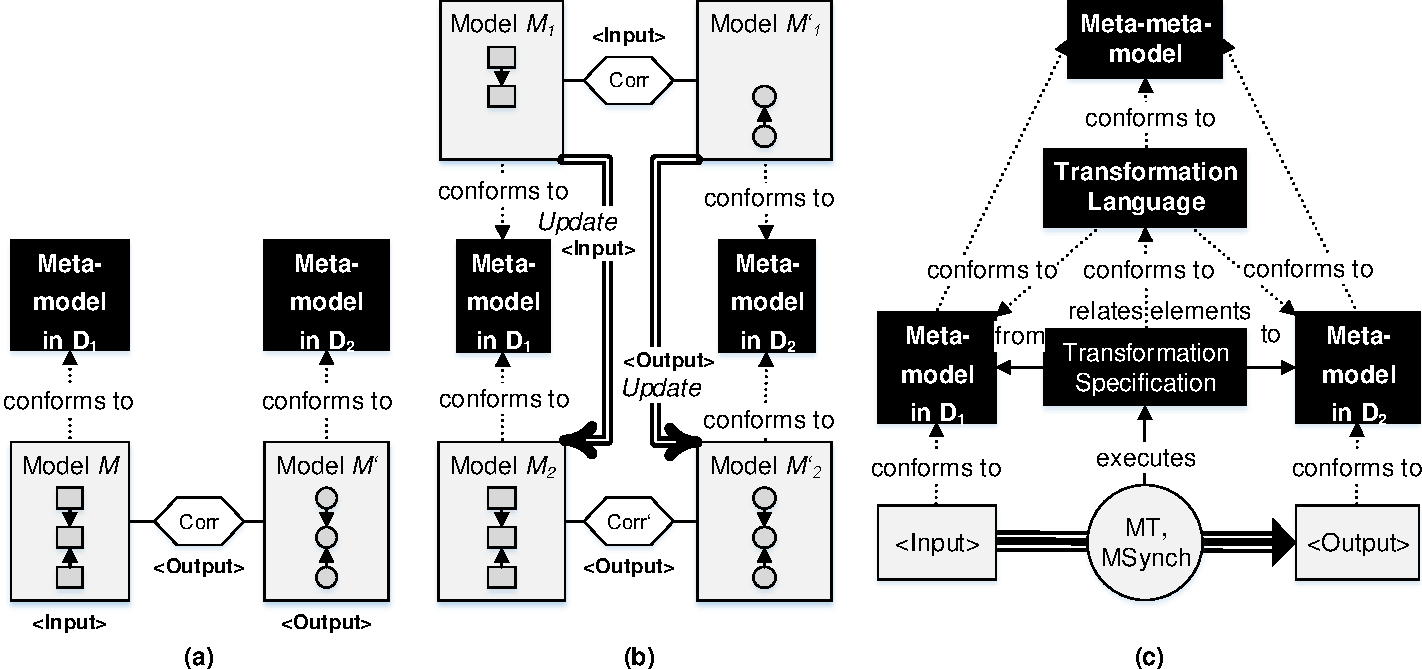
\includegraphics[width=\textwidth]{img/gen_intro/mt_msynch.pdf}};
\fill (-.8,1.2) node[inner sep=1pt] (B) {\small{$\delta$}};
\fill (.1,-.5) node[inner sep=1pt] (C) {\small{$\delta'$}};
\end{tikzpicture}
\end{center}
\caption{Setting of Model Transformations (a), Model Synchronisations (b) \& their Execution (c) (Adaption from \cite{FAGT2,Lucio2014})}
\label{fig:sec-gen-intro-msynch:mt_msynch}
\end{figure}

\cref{fig:sec-gen-intro-msynch:mt_msynch} (c) illustrates the execution of a model transformation that takes a source model $M \in \Lang(D_1)$ over the meta-model in source domain $D_1$ as input and outputs a target model $M' \in \Lang(D_2)$ over the meta-model in target domain $D_2$ together with a correspondence (\code{Corr}) which relates elements from $M$ to $M'$ as depicted in \cref{fig:sec-gen-intro-msynch:mt_msynch} (a).
The model transformation (MT) is performed by executing the model transformation specification.
The specification is defined based on the two meta-models in domains $D_1$ and $D_2$ and defines which model elements in $D_1$ should be transformed to which model elements in $D_2$ by relating (mapping) model elements from $D_1$ to $D_2$.
The transformation specification is expressed in (conforms to) a transformation language.
The transformation language contains (allows to express) the set of all conceivable mappings of model elements from $D_1$ to $D_2$.
Therefore, the transformation language conforms to the meta-models in domains $D_1$ and $D_2$ which in turn conform to a common meta-meta-model (cf. \cref{fig:sec-gen-intro-mt:meta}), i.e., the transformation language indirectly conforms to this meta-meta-model.
Although, both meta-models may conform to different meta-meta-models in general, the assumption of a common meta-meta-model of class diagrams is valid as already discussed.

Different model transformation approaches and tools \cite{HLG13+,Rose2014} do exist.
Beside model transformation by-example \cite{Kappel2012} where the transformation specification is generated from a given source model, target model and their correspondence, different types of transformation languages exist for explicitly specifying the transformation \cite{Guerra2013}, e.g., QVT \cite{QVT}, ATL \cite{Jouault200831}, triple graph grammars (TGGs) \cite{DBLP:journals/eceasst/AnjorinLS15} and ETL \cite{Kolovos2008}.
Different types of transformation languages may allow transformation specifications in textual or visual form and in declarative or operational manner \cite{tm13}.
While declarative transformation specifications focus on the specific mapping of model elements between domains, operational specifications additionally provide the concrete steps how the target model is derived from a source model, e.g., by providing the concrete order of traversing the model elements of the source model.
Furthermore, we distinguish between in-place model transformations and ``external" transformations where the source model is preserved by the transformation while the target model is constructed in parallel.
Moreover, model-to-model transformations are distinguished from model-to-text, text-to-model and text-to-text transformations.
However, note that any of these types of transformations can be simulated by ``external'' model-to-model transformations where the parallel target model is taken as output of an in-place transformation and text is parsed to (serialised from) a model before (after) executing the model-to-model transformation.
Therefore, we focus on ``external" model-to-model transformations based on TGGs that allow visual, declarative transformation specifications.
We review basic concepts and notions in \cref{sec-tgg,sec-mt-tgg}.
Beside the model-to-model transformation CD2RDBM from UML class diagrams to relational database models in \ref{sec-mt-tgg}, we present software transformations, i.e., text-to-(text)model transformations, from source code to visual models (or source code again) in \cref{sec-compl-software-trans}.


\subsection{Model Synchronisation}
\label{sec-gen-intro-msynch}
Basically, model synchronisations $\MSynch\colon \Delta_{D_1} \to \Delta_{D_2}$ are performed based on model transformations where model updates $\delta \in \Delta_{D_1}$ in domain $D_1$ are propagated (mapped) to (model updates $\delta' \in \Delta_{D_2}$ in) domain $D_2$ by performing model transformations.
Therefore, the classification of model transformations from \cref{sec-gen-intro-mt} can also be applied to model synchronisations, i.e., model synchronisations may be
\begin{enumerate*}
\item endogenous or exogenous,
\item horizontal or vertical,
\item based on textual or visual transformation specifications,
\item based on declarative or operational transformation specifications, and
\item propagations of updates from model-to-model, model-to-text, text-to-model or text-to-text.
\end{enumerate*}

According to \cref{fig:sec-gen-intro-msynch:mt_msynch} (b), a model update in some domain $D$ relates model $M_1 \in \Lang(D)$ from before the update with model $M_2 \in \Lang(D)$ from after performing the update and therefore, the update documents the changes to $M_1$ which have led to $M_2$.
Thus, a model update relates models that are expressed in the same DSL $\Lang(D)$, i.e., models $M_1$ and $M_2$ conform to the same meta-model in domain $D$.
\cref{fig:sec-gen-intro-msynch:mt_msynch} (c) illustrates the execution of a model synchronisation that takes a model update $\delta$ in source domain $D_1$ from model $M_1$ to model $M_2$ as input together with a correspondence (\code{Corr}) which interrelates model $M_1$ with model $M'_1$ in target domain $D_2$ to which the update should be propagated.
The execution outputs an update $\delta'$ in target domain $D_2$ from model $M'_1$ to model $M'_2$ together with a correspondence (\code{Corr'}) which relates model $M_2$ with model $M'_2$.
The model synchronisation (MSynch) is performed based on executing the model transformation specification.

According to \cref{sec-gen-intro-mt}, we focus on model-to-model synchronisations based on TGGs that allow visual, declarative transformation specifications.
We review basic concepts and notions in \cref{sec-tgg,sec-msynch-tgg}.
Beside the model-to-model propagation of model updates from UML class diagrams to relational database models in \cref{sec-msynch-tgg}, we present software synchronisations, i.e., text-to-model(text) propagations of updates from source code to visual models (or source code again) in \cref{sec-compl-software-synch}.


\section{Graph Transformation}
\label{sec-gen-intro-gt}

We recall basic definitions and results of the theory of algebraic graph transformation from \cite{Ehrig:2006:FAG:1121741,FAGT2}.
In particular this includes the category $\AGraphs_\ATGI$ of typed attributed graphs with node type inheritance from \cite{DBLP:journals/tcs/GolasLEO12,FAGT2} in \cref{sec-gt-graphs}, their transformation and the generalisation to $\M$-adhesive transformation systems from \cite{FAGT2} in \cref{sec-gt-trafo}.
Furthermore, we review the notions of (nested) graph conditions and constraints as well as their interpretation via AC-schemata from \cite{DBLP:journals/mscs/HabelP09,FAGT2} in \cref{sec-gt-gc}.
Moreover, in \cref{prop:sec-gc-gc:rel_sat_cond_ac} we show that the direct interpretation of type strict conditions coincides with their interpretation via AC-schemata when restricting to $\M$-matches.
For the general case, in \cref{th:sec-gc-gc:rel_sat_ac_schema} we show that the standard satisfiability of an AC-schema coincides with the $\morO$-satisfiability of the underlying condition.
This allows an interpretation of conditions via $\morO$-matches and $\morO$-satisfiability from a user point of view while an interpretation via the standard satisfiability of AC-schemata with $\M$-matches is used to prove technical results.

\subsection{Graphs, Typed \& Attributed Graphs}
\label{sec-gt-graphs}
\begin{figure}[!tb]
\begin{center}
\begin{tikzpicture}[]
\fill (0,0) node[inner sep=1pt] (A) {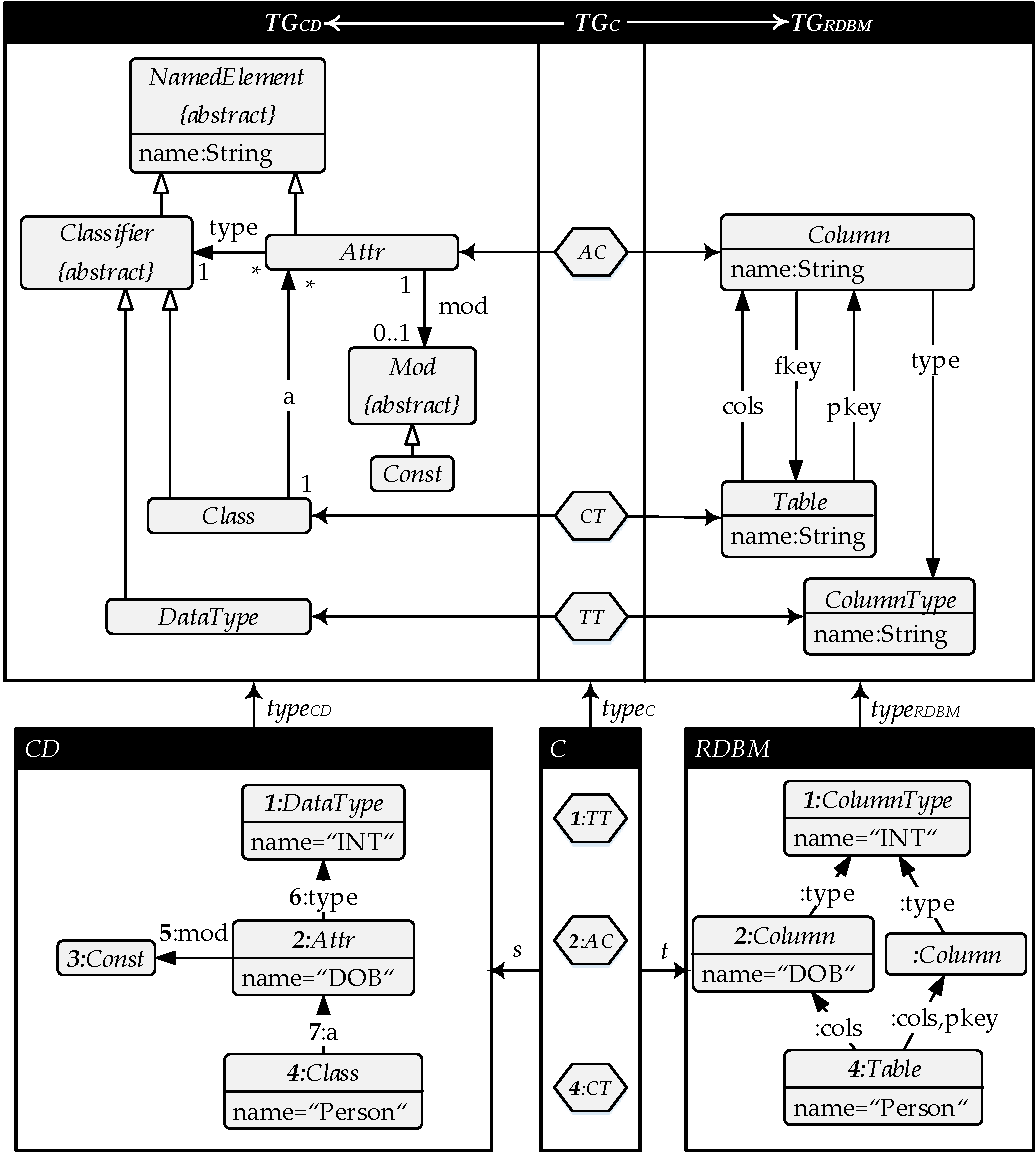
\includegraphics[width=.9\textwidth]{img/gen_intro/atg.pdf}};
%\fill (-2.5,7.55) node[inner sep=1pt] (B) {\textcolor{white}{$(\TG_\CD \gets \Corr \to \TG_\RDBM)$}};
\end{tikzpicture}
\end{center}
\caption{Attributed Triple Type Graph $(\TG_\CD \gets \TG_C \to \TG_\RDBM)$ (top) \& Typed Attributed Triple Graph $(\CD \transB{s} C \trans{t} \RDBM)$ (bottom)}
\label{fig:sec-gt-graphs:atg}
\label{fig:mm}
\end{figure}

We assume that (visual) models are represented by graphs (cf. \cref{sec-gen-intro-gratrafo}).
A plain graph consists of nodes (vertices) and edges between nodes.
An edge links a source node with a target node.
The presented notion of graphs allows parallel edges between two nodes and edge loops.
A morphism $f\colon G_1 \to G_2$ from a graph $G_1$ to a graph $G_2$ is a mapping from nodes and edges in $G_1$ to nodes and edges in $G_2$ such that the structure of $G_1$ is preserved, i.e, the source (target) node of each edge $e$ in $G_1$ is mapped to the source (target) node of edge $f(e)$ in $G_2$.

\begin{definition}[Graph and Graph Morphism (Def. 2.1 in \cite{FAGT2})]
A \emph{graph}\index{graph} $G=(V_G,E_G,s_G\colon E_G \to V_G,t_G\colon E_G \to V_G)$ consists of a set of nodes $V_G$, a set of edges $E_G$ and two functions $s_G,t_G$ that map the source node (via $s_G$) and target node (via $t_G$) to each edge.
A \emph{graph morphism}\index{graph!morphism} $f\colon G_1 \to G_2$ from $G_1$ to $G_2$ with $f=(f_V,f_E)$ consists of two functions $f_V\colon V_{G_1} \to V_{G_2},f_E\colon E_{G_1} \to E_{G_2}$ such that $s_{G_2} \circ f_E=f_V \circ s_{G_1}$ and $t_{G_2} \circ f_E=f_V \circ t_{G_1}$.
\envEndMarker
\end{definition}

A typed graph is a plain graph $G$ together with a graph morphism from $G$ to a distinguished type graph $\TG$ that defines the typing of each node and edge in $G$ - We say that $G$ is typed over $\TG$.
Therefore, a type graph is part of the meta-model for a given domain and defines the concepts (node types) for the domain and their interrelationships (edge types) that can be used in graphs as models in the domain (cf. \cref{sec-gen-intro-mt,fig:sec-gen-intro-mt:meta}).
A typed graph morphism between two typed graphs is a graph morphism that additionally preserves the typing.

\parpic[r][r]{
$
\SelectTips{cm}{}
     \xymatrix@R-3.3ex@C-2ex{
     G_1 \ar[rr]^{f} \ar[dddr]_{\type_{G_1}} & \ar@{}[dd]|{(=)} & G_2 \ar[dddl]^{\type_{G_2}} \\
     & & \\
     & & \\
     & \TG & \\
     }
$
}
\vspace{-1.5ex}

\begin{definition}[Typed Graph and Typed Graph Morphism (Def. 2.2 in \cite{FAGT2})]
\label{def:sec-gt-graphs:typed_graphs}
Given a distinguished graph $\TG$ as the type graph.
A \emph{typed graph $G^\T=(G,\type_G\colon G \to \TG)$ over $\TG$}\index{graph!typed} is given by a graph $G$ and a graph morphism $\type_G$ from $G$ to $\TG$.
A \emph{typed graph morphism}\index{graph!morphism!typed} $f\colon G^\T_1 \to G^\T_2$ is a graph morphism $f\colon G_1 \to G_2$ such that $\type_{G_2} \circ f=\type_{G_1}$.
\envEndMarker
\end{definition}

Attributed graphs are defined based on the notion of E-graphs that allow the attribution of edges and nodes.
The set of possible attribute values is defined by an algebra.
For an introduction to algebraic signatures and algebras we refer to \cite{Ehrig:2006:FAG:1121741}.

\parpic[r][r]{
$
\SelectTips{cm}{}
     \xymatrix@R-3.3ex@C-2ex{
     & E^G_G \ar@/^/[rr]^{s^G_G} \ar@/_/[rr]_{t^G_G} & & V^G_G & \\
     & & & & \\
     & & & & \\
     E^G_{EA} \ar[uuur]^{s^G_{EA}} \ar[rr]^{t^G_{EA}} & & V^G_D & & E^G_{NA} \ar[uuul]_{s^G_{NA}} \ar[ll]_{t^G_{NA}} \\
     }
$
}
\vspace{-1.5ex}

\begin{definition}[Attributed Graph and Attributed Graph Morphism (Def. 2.4 in \cite{FAGT2})]
\label{def:sec-gt-graphs:agraphs}
An \emph{E-graph}\index{graph!E-graph} $G^\EE=(V_G^G,V_D^G,E_G^G,E_{NA}^G,E_{EA}^G,(s_i^G,t_i^G)_{i \in \{G,NA,EA\}})$ with graph nodes $V_G^G$, data nodes $V_D^G$, graph edges $E_G^G$, node attribute edges $E_{NA}^G$, edge attribute edges $E_{EA}^G$ and source and target functions $s_i^G,t_i^G$ with signatures as defined on the right.
An \emph{E-graph morphism}\index{graph!morphism!E-graph} $f\colon G^\EE_1 \to G^\EE_2$ with $f=((f_{V_i}\colon V_i^{G_1} \to V_i^{G_2})_{i \in \{G,D\}}, (f_{E_j}\colon E_j^{G_1} \to E_j^{G_2})_{j \in \{G,NA,EA\}})$ is a pair of tuples of functions $f_{V_i}$ for mapping nodes and functions $f_{E_j}$ for mapping edges from $G^\EE_1$ to $G^\EE_2$ such that $f$ commutes with all source and target functions.
Given a data signature $\DSIG=(S,\OP)$, then an \emph{attributed graph over $\DSIG$}\index{graph!attributed} is given by $G=(G^\EE,D_G)$ with $G^\EE$ being an E-graph and $D_G$ being a $\DSIG$-algebra such that $\dot{\cup}_{s \in S}(D_{G,s})=V^G_D$.
Given attributed graphs $G_1$ and $G_2$ over common $\DSIG$, then an \emph{attributed graph morphism}\index{graph!morphism!attributed} $f\colon G_1 \to G_2$ from $G_1$ to $G_2$ with $f=(f_G,f_D)$ is a pair of an E-graph morphism $f_G\colon G^\EE_1 \to G^\EE_2$ and an algebra homomorphism $f_D\colon D_{G_1} \to D_{G_2}$ such that $f_{G,V_D}(x)=f_{D,s}(x)$ for all $x \in D_{G_1,s},s \in S$.
\index{graph!attributed!graph part}\index{graph!attributed!data part}With $(V^G_G,(E^G_X)_{X \in \{G,NA,EA\}})$ we refer to the (structural) graph part of attributed graph $G$ and distinguish it from its data part $(V^G_D,D_G)$.
\index{graph!morphism!attributed -- graph part}\index{graph!morphism!attributed -- data part}With $f_S=(f_{G,V_G},f_{G,E_G},f_{G,E_{NA}},f_{G,E_{EA}})$ we refer to the (structural) graph part of attributed graph morphism $f$ and distinguish it from its data part $f_D$.
\envEndMarker
\end{definition}

Typed and attributed graphs (morphisms) are combined to typed attributed graphs (morphisms).

\begin{definition}[Typed Attributed Graph and Morphism (Def. 2.5 in \cite{FAGT2})]
\label{def:sec-gt-graphs:typed_attr_graphs}
Given a distinguished attributed graph $\ATG=(\TG,Z)$ as attributed type graph with $Z$ being the final $\DSIG$-algebra.
The final $\DSIG$-algebra \index{final $\DSIG$-algebra}contains exactly one element in each carrier set.
A \emph{typed attributed graph \index{graph!typed \& attributed} $G^\T=(G,\type_G\colon G \to \ATG)$ over $\ATG$} is given by an attributed graph $G$ over $\DSIG$ and an attributed graph morphism $\type_G$ from $G$ to $\ATG$.
Given typed attributed graphs $G^\T_1$ and $G^\T_2$ over common $\ATG$, then a \emph{typed attributed graph morphism}\index{graph!morphism!typed \& attributed} $f\colon G^\T_1 \to G^\T_2$ is an attributed graph morphism $f\colon G_1 \to G_2$ such that $\type_{G_2} \circ f=\type_{G_1}$.
\envEndMarker
\end{definition}

\begin{remark}[Typed Attributed Graphs with Node Type Inheritance]
\label{rem:sec-gt-graphs:inheritance}
Typed attributed graphs and morphisms are extended to typed attributed graphs and morphisms with node type inheritance.
Therefore, the type graph is extended with an additional inheritance relation between nodes that defines which nodes in the type graph inherit from which other nodes.
Furthermore, nodes in the type graph can be explicitly marked as abstract, i.e., abstract nodes cannot be directly used as concrete types for nodes in graphs that are typed over this type graph.
A node \code{A} that inherits from a node \code{B} shares all node attributes as well as incoming and outgoing edges of \code{B} with \code{B}.
If node \code{A} inherits from node \code{B}, then \code{A} is called the sub-node (sub-type) of \code{B} whereas \code{B} is called the super-node (super-type) of \code{A}.
A morphism between two typed attributed graphs $G_1$ and $G_2$ with node type inheritance may refine the types of nodes from $G_1$ to $G_2$ by mapping nodes in $G_1$ of super-type \code{B} to nodes in $G_2$ of sub-type \code{A}.
Basically beside abstract nodes, typed graphs with node type inheritance do not lead to additional expressiveness in comparison to graphs without node type inheritance, since, the type graph with inheritance can most widely be flattened to a type graph without inheritance information by duplicating edges and attributes from super-nodes to sub-nodes (cf. Def. 6 in \cite{DBLP:journals/tcs/GolasLEO12}). 
However, type graphs with inheritance allow a more compact notation in comparison to their flattened versions (cf. Figs. 1 and 4 in \cite{DBLP:journals/tcs/GolasLEO12}).
We allow inheritance in type graphs and refer to \cite{DBLP:journals/tcs/GolasLEO12} for technical details.
\envEndMarker
\end{remark}

\begin{example}[Attributed Type Graph \& Typed Attributed Graph]
\label{ex:sec-gt-graph:type_graph}
\cref{fig:sec-gt-graphs:atg} depicts attributed type graphs $\TG_\CD$ and $\TG_\RDBM$ for class diagrams ($\CD$) and relational database models ($\RDBM$).
Both type graphs are part of the meta-models for the domains of CDs and RDBMs.
Class diagrams may contain several \code{Class}es, each with a set of class \code{Attr}ibutes that are assigned via \code{a} edges to the class.
Furthermore, each attribute is \code{type}d by a \code{Classifier}.
By node type inheritance, classifiers are classes or other \code{DataType}s.
Furthermore by node type inheritance, each class, attribute and data type is a \code{NamedElement} and therefore has a specific \code{name} of type \code{String}.
Moreover, attributes may have a \code{Mod}ifier \code{Const}ant which declares that the attribute value does not change.
Note that nodes \code{NamedElement}s, \code{Classifier}s and \code{Mod}ifiers are marked as \code{abstract} and therefore, they cannot be directly used as concrete types in class diagrams but their sub-nodes (sub-types).

Relational database models may contain several \code{Table}s.
A table has a \code{name} of type \code{String} and may have several \code{Column}s assigned via \code{cols} edges where one column may contain the primary keys of the rows of the table (edge \code{pkey}) or columns may refer to other tables by foreign keys (\code{fkey}).
Furthermore, each column has a specific \code{name} of type \code{String} and is of a specific \code{type}.
Analogously, each column type has a \code{name} of type \code{String}.

The multiplicity constraints on the edges in type graph $\TG_\CD$ are expressed by graph constraints in \cref{sec-gt-gc,ex:sec-gc-gc:gc_UML_CD} and complete the meta-model for the domain of UML class diagrams.

Typed attributed graph $\CD$ ($\RDBM$) is a class diagram (relational database model) typed over type graph $\TG_\CD$ ($\TG_\RDBM$) via morphism $\type_\CD$ ($\type_{\RDBM}$).
The class diagram $\CD$ contains a class of name \code{``Person''} together with a class attributes \code{``DOB''} (date of birth) of type \code{``INT''}.
Furthermore, attribute \code{``DOB''} is equipped with modifier \code{Const} (constant).
For typing, node \code{2} in $\CD$ is mapped to node \code{Attr} in $\TG_\CD$ along morphism $\type_\CD$.
All other nodes, edges and node attributes in $\CD$ are mapped analogously.
The formal notation of graph $\CD$ is given below:
\paragraph*{}
$\CD=(\underline{\CD},\type_{\underline{\CD}}\colon \underline{\CD} \to \TG_\CD)$ where $\underline{\CD}=(\underline{\CD}^E=(V_G^{\underline{\CD}},V_D^{\underline{\CD}},E_G^{\underline{\CD}},E_{NA}^{\underline{\CD}},E_{EA}^{\underline{\CD}},$ $(s_i^{\underline{\CD}},t_i^{\underline{\CD}})_{i \in \{G,NA,EA\}}),D_{\underline{\CD}})$ with 
\newline
$V_G^{\underline{\CD}}=\{1,2,3,4\},$
\newline
$V_D^{\underline{\CD}}=D_{\underline{\CD},String},$
\newline
$E_G^{\underline{\CD}}=\{5,6,7\},$
\newline
$E_{NA}^{\underline{\CD}}=\{a,b,c\},$
\newline
$E_{EA}^{\underline{\CD}}=\{\},$
\newline
$s_G^{\underline{\CD}}=(5 \mapsto 2,6 \mapsto 2,7 \mapsto 4),$
\newline
$t_G^{\underline{\CD}}=(5 \mapsto 3,6 \mapsto 1,7 \mapsto 2),$
\newline
$s_{NA}^{\underline{\CD}}=(a \mapsto 1,b \mapsto 2, c \mapsto 4),$
\newline
$t_{NA}^{\underline{\CD}}=(a \mapsto ``INT'',b \mapsto ``DOB'',c \mapsto ``Person''),$
\newline
$s_{EA}^{\underline{\CD}}=t_{EA}^{\underline{\CD}}=\varnothing,$
\newline
$D_{\underline{\CD}}=(D_{\underline{\CD},String}=\{w^* \mid w \in \{a..z,A..Z\}\},OP_{D_{\underline{\CD}}}=\varnothing)$ being a $\DSIG$-algebra for algebraic data signature $\DSIG=(S=\{String\},OP=\varnothing),$ and
\newline
$\type_{\underline{\CD}}=(\type_{\underline{\CD},G}=(\type_{\underline{\CD},V_G},\type_{\underline{\CD},V_D},\type_{\underline{\CD},E_G},\type_{\underline{\CD},E_{NA}},\type_{\underline{\CD},E_{EA}}),\type_{\underline{\CD},D}\colon D_{\underline{\CD}} \to D_{\TG_\CD})$ being the type morphism with
\newline
$\type_{\underline{\CD},V_G}=(1 \mapsto DataType,2 \mapsto Attr,3 \mapsto Const,4 \mapsto Class),$
\newline
$\type_{\underline{\CD},V_D}(x)=\type_{\underline{\CD},D,String}(x),\forall x \in D_{\underline{\CD},String},$
\newline
$\type_{\underline{\CD},E_G}=(5 \mapsto mod,6 \mapsto type,7 \mapsto a),$
\newline
$\type_{\underline{\CD},E_{NA}}=(a,b,c \mapsto name),$
\newline
$\type_{\underline{\CD},E_{EA}}=\varnothing,$ and
\newline
$\type_{\underline{\CD},D,String}(x)=String,\forall x \in D_{\underline{\CD},String}$ for final $\DSIG$-algebra $D_{\TG_\CD}=(D_{\TG_\CD,String}=\{String\},OP_{D_{\TG_\CD}}=\varnothing)$ of attributed type graph $\TG_\CD$.

The relational database model $\RDBM$ contains a corresponding \code{Table}, \code{Column} and \code{ColumnType} for each \code{Class}, \code{Attr}ibute and \code{DataType} of class diagram $\CD$.
The formal notation of typed attributed graph $\RDBM$ is analogously to $\CD$.
\envEndMarker
\end{example}

\paragraph*{Visual Notation}
\label{par:sec-gt-graphs:vis}
As depicted in \cref{fig:sec-gt-graphs:atg}, nodes (edges) in typed graphs are visualised by \code{x:y} with \code{x} being the name of the node (edge) and \code{y} being the type of the node (edge).
The mapping of nodes and edges along morphisms correspond to their naming in visual notation, e.g., in visualisations of graph conditions, graph transformation rules, triple graphs and model updates (cf. \cref{sec-gt-gc,sec-gt-trafo,sec-tgg,sec-msynch-tgg}).
We omit node and edge names in visualisations if they are irrelevant and write \code{:y} instead of \code{x:y}.
Note that in formal notation of attributed graphs, node (and edge) attributes are edges and attribute values are nodes.
However, in visual notation we write \code{attr=x} for attribute \code{attr} with value \code{x} directly in the corresponding node (or edge) shape.
For an explicit visualisation of attributed graphs in E-graph notation we refer to Ex. 8.5 in \cite{Ehrig:2006:FAG:1121741}.
Although technically, a node or edge may have the same attribute several times (with possibly different attribute values), usually in practice, each node and edge has each attribute at most once such that the mapping of attributes and their values along morphisms is clear and is not explicitly visualised.

\subsection{$\M$-adhesive Categories}
\label{sec-gt-M-adh}
In the following, we review the notion of $\M$-adhesive categories as a generalisation of the category of typed attributed graphs.
For a short introduction to category theory we refer to \cite{Ehrig:2006:FAG:1121741} and for a more detailed view we refer to \cite{Ehrig:1990:FAS:77299,Adamek:1990:ACC:78162}.

\begin{remark}[Basic Notions of Category Theory \& Category $\AGraphs_\ATGI$]
\label{rem:sec-gt-M-adh}
\emph{A category $\cat{C}=(\ob_\cat{C},\morB_\cat{C},\circ,\id)$}\index{category} is defined by a class $\ob_\cat{C}$ of objects, a set $\morB_\cat{C}$ of morphisms $f\colon A \to B$ between objects $A,B \in \ob_\cat{C}$, for all objects $A,B,C \in \ob_\cat{C}$ and morphisms $f\colon A \to B,g\colon B \to C \in \morB_\cat{C}$ a composition $g \circ f \in \morB$, and for each object $A \in \ob_\cat{C}$ an identity morphism $\id_A\colon A \to A \in \morB_\cat{C}$ such that
\begin{enumerate*}
\item [``Associativity:''] For all objects $A,B,C,D \in \ob_\cat{C}$ and morphisms $f\colon A \to B,g\colon B \to C,h\colon C \to D \in \morB_\cat{C}$ it holds that $(h \circ g) \circ f=h \circ (g \circ f)$, and
\item [``Identity:''] For all objects $A,B \in \ob_\cat{C}$ and morphisms $f\colon A \to B \in \morB_\cat{C}$ it holds that $f \circ \id_A=f$ and $\id_B \circ f=f$ (cf. Def. A.1 in \cite{Ehrig:2006:FAG:1121741}).
\end{enumerate*}
A functor \index{functor} $F\colon \cat{C} \to \cat{D}$ is a mapping from objects and morphisms of category \cat{C} to objects and morphisms of category \cat{D} which is compatible with composition and the identities (cf. A.6 in \cite{Ehrig:2006:FAG:1121741}).
Inclusions $i\colon A \to B$ are morphisms with $i(A)=A$\index{inclusion}.
With \emph{mono- epi- and iso-morphisms}\index{morphism!monomorphism}\index{morphism!epimorphism}\index{morphism!isomorphism} we denote special types of morphisms in categories $\cat{C}$.
Intuitively, an isomorphism is a morphism between two objects of the same structure that additionally preserves this structure.
According to Def. A.9 in \cite{Ehrig:2006:FAG:1121741}, morphism $f\colon A \to B \in \morB_\cat{C}$ is an isomorphism, if there exists an inverse morphism $f^{-1}\colon B \to A \in \morB_\cat{C}$ such that $f^{-1} \circ f=\id_A$ and $f \circ f^{-1}=\id_B$.
In this context, the inverse morphism $f^{-1}$ is unique and also an isomorphism (cf. Rem. A.10 in \cite{Ehrig:2006:FAG:1121741}) and the composition $i_2 \circ i_1$ of two isomorphisms $i_1,i_2$ is again an isomorphism.
We write $G \cong G'$ and say that $G$ is isomorphic to $G'$, if there exists an isomorphism $i\colon G \to G'$.
According to Def. A.12 in \cite{Ehrig:2006:FAG:1121741}, mono- and epi-morphisms are defined as follows.
A morphism $h\colon B \to C \in \morB_\cat{C}$ is a monomorphism, if for all morphisms $f,g\colon A \to B \in \morB_\cat{C}$ it holds that $h \circ f=h \circ g$ implies $f=g$.
Conversely, a morphism $f\colon A \to B \in \morB_\cat{C}$ is an epimorphism, if for all morphisms $g,h\colon B \to C \in \morB_\cat{C}$ it holds that $g \circ f=h \circ f$ implies $g=h$.
Note that an isomorphism is both an epi- and monomorphism but a morphism that is an epi- and monomorphism must not be an isomorphism in general, since, the inverse morphism may not exist.
According to Def. A.16 in \cite{FAGT2}, a morphism pair $(f_1\colon A_1 \to B,f_2\colon A_2 \to B)$ is jointly epimorphic\index{morphism!epimorphism!jointly}, if for all morphisms $g,h\colon B \to C$ it holds that $g \circ f_i=h \circ f_i$ for $i=1,2$ implies $g=h$.
Given the category $\AGraphs_\ATGI$\index{category!$\AGraphs_\ATGI$} with all typed attributed graphs over attributed type graph $\ATGI$ with node type inheritance as objects and all typed attributed graph morphisms between them as morphisms where furthermore, the identities are given by the componentwise identities on nodes, edges, attributes and algebras and the composition $g \circ f$ is given by $g(f(x))$ componentwise for all nodes, edges, attributes and elements $x$ of carrier sets in the corresponding algebra (cf. \cref{sec-gt-graphs,def:sec-gt-graphs:typed_attr_graphs}).
Then, the monomorphisms\index{category!$\AGraphs_\ATGI$!monomorphism} are exactly those morphisms that are componentwise injective, the epimorphisms\index{category!$\AGraphs_\ATGI$!epimorphism} are exactly those morphisms that are componentwise surjective and isomorphisms\index{category!$\AGraphs_\ATGI$!isomorphism} are exactly those morphisms that are componentwise bijective (i.e., both injective and surjective) (cf. Fact 2.15 in \cite{Ehrig:2006:FAG:1121741}).
The jointly epimorphic pairs of morphisms are exactly those pairs that are together surjective.
Basic constructions in categories are pushouts and pullbacks.\index{pushout}\index{pullback}
A pushout $B +_A C$ is the gluing of objects $B,C$ via common sub-object $A$.
In $\AGraphs_\ATGI$, if $A=\varnothing$ is the empty graph $\varnothing$, then $B +_A C$ is the componentwise disjoint union of graphs $B$ and $C$.
In contrast, a pullback is the intersection of objects $B$ and $C$ via common object $D$.
\parpic[r][r]{
\SelectTips{cm}{}
$
\xymatrix@C-2ex@R-2ex{
X \ar[rd]|{x} \ar[rrrd]|{h_X} \ar[dddr]|{k_X} & & & & \\
  & A \ar[rr]|{f} \ar[dd]|{g} & & B \ar[dd]|{g'} \ar[rddd]|{h_Y} & \\
  & & (1) & & \\
  & C \ar[rr]|{f'} \ar[rrrd]|{k_Y} & & D \ar[rd]|{y} & \\
  & & & & Y
}
$
}
\emph{A pushout (PO) $(1)$ or $(f',g')$ over morphisms $(f,g)$}, written $B +_A C$, is defined by
\begin{enumerate*}
\item a pushout object $D$, and
\item morphisms $f',g'$ with $f' \circ g=g' \circ f$, such that the following universal property is fulfilled: for all objects $Y$ and morphisms $h_Y,k_Y$ with $k_Y \circ g=h_Y \circ f$, there is a unique morphism $y\colon D \to Y$ such that $y \circ g'=h_Y$ and $y \circ f'=k_Y$ (cf. Def. A.17 in \cite{Ehrig:2006:FAG:1121741}).
\end{enumerate*}
Note that the pushout object is unique up to isomorphism (cf. Rem. A.18 in \cite{Ehrig:2006:FAG:1121741}) and furthermore, $(f',g')$ is jointly epimorphic.
According to Def. A.20 in \cite{Ehrig:2006:FAG:1121741}, for pushout $(1)$, \emph{$(f',g)$ is called the pushout complement over $(f,g')$}\index{pushout!complement}.
The ``smallest'' pushout (1) with $f,f' \in \M$ for a given morphism $g'$ is called initial pushout for $g'$.
In categories of graphs, the initial pushout (1) is the smallest pushout for $g'$ in the sense that boundary graph $A$\index{pushout!initial!boundary graph} only contains those graph elements of $B$ that are necessary to glue $B$ and context graph $C$\index{pushout!initial!context graph} via common $A$ to $D$.
For technical details we refer to Def. 4.23, item 4 in \cite{FAGT2}.\index{pushout!initial}
The pushout complement over $(h_X,g')$ exists if and only if for the initial pushout (1) for $g'$, there is a morphism $b^*\colon A \to X$ such that $h_X \circ b^*=f$ (cf. Thm. 6.4 in \cite{Ehrig:2006:FAG:1121741}).\index{pushout!complement!existence}
\emph{A pullback (PB) $(1)$ or $(f,g)$ over morphisms $(f',g')$} is defined by
\begin{enumerate*}
\item a pullback object $A$, and
\item morphisms $f,g$ with $g' \circ f=f' \circ g$, such that the following universal property is fulfilled: for all objects $X$ and morphisms $h_X,k_X$ with $f' \circ k_X=g' \circ h_X$, there is a unique morphism $x\colon X \to A$ such that $f \circ x=h_X$ and $g \circ x=k_X$ (cf. Def. A.22 in \cite{Ehrig:2006:FAG:1121741}).
\end{enumerate*}
With diagram $(1)$ commutes we mean that $g' \circ f=f' \circ g$.
With $(1)+(2)$ we denote the composition of two adjacent diagrams.
\envEndMarker
\end{remark}

$\M$-adhesive categories are defined based on the following properties.
For $\M$-morphisms $m$, we write $m \in \M$ and say that $m$ is in $\M$.
For several $\M$-morphisms $m_1,\ldots,m_n$ we write $m_1,\ldots,m_n \in \M$.

\begin{definition}[PO-PB compatibility (Def. 4.2 \& Rem. 4.3 in \cite{FAGT2})]
\label{def:sec-gt-M-adh:PO-PB-comp}
A morphism class $\M$ in a category $\cat{C}$ is called \emph{PO-PB compatible}\index{$\M$-morphisms} if
\begin{enumerate}
  \item $\M$ is a class of monomorphisms, contains all identities (and isomorphisms), is closed under composition ($\M$-composition\index{$\M$-composition}), i.e., $(f\colon A \to B \in \M,g\colon B \to C \in \M \implies g \circ f \in \M)$, and is closed under decomposition ($\M$-decomposition\index{$\M$-decomposition}), i.e., $g \circ f \in \M, g \in \M$ implies $f \in \M$.
  \item $\cat{C}$ has pushouts and pullbacks along $\M$-morphisms (i.e., if $f \in \M$ or $g \in \M$ ($f' \in \M$ or $g' \in \M$), then there is a pushout (pullback) $(1)$), and $\M$-morphisms are closed under pushouts and pullbacks (i.e., $\M$-morphisms are preserved by pushouts and pullbacks - for pushout (pullback) $(1)$, if $f \in \M$ ($f' \in \M$), then $f' \in \M$ ($f \in \M$)).
\end{enumerate}
\envEndMarker
\end{definition}

For $\M$-van Kampen squares, we refer to Def. 4.1 in \cite{FAGT2}.

\begin{definition}[$\M$-adhesive Category (Def. 4.4 in \cite{FAGT2})]
\label{def:sec-gt-M-adh:M-adh-cat}
A category $\cat{C}$ with a PO-PB compatible morphism class $\M$ is called an \emph{$\M$-adhesive category $(\cat{C},\M)$}\index{category!$\M$-adhesive} if pushouts in $\cat{C}$ along $\M$-morphisms are $\M$-van Kampen squares.
\envEndMarker
\end{definition}

In addition to the properties in \cref{def:sec-gt-M-adh:PO-PB-comp,def:sec-gt-M-adh:M-adh-cat}, the following basic HLR properties hold for $\M$-adhesive categories (we only list those basic HLR properties that are used in proofs of results of this thesis - For a complete list we refer to Def. 4.21 in \cite{FAGT2}).

\begin{definition}[Basic HLR properties (Thm. 4.22 in \cite{FAGT2})]
\label{def:sec-gt-M-adh:hlr_props}
\index{category!$\M$-adhesive!basic HLR properties}
Given an $\M$-adhesive category $(\cat{C},\M)$, then the following properties are valid:
\begin{itemize}
  \parpic[r][r]{
$
\SelectTips{cm}{}
     \xymatrix@R-3.3ex@C-2ex{
     A \ar[dd]_{l} \ar[rr]^{k} & & B \ar[rr]^{r} \ar[dd]^{s} & & E \ar[dd]^{v} \\
     & (1) & & (2) & \\
     C \ar[rr]_{u} & & D \ar[rr]_{w} & & F\\
     }
$
}
  \item Pushouts along $\M$-morphisms are pullbacks, i.e., given pushout $(1)$ with $k \in \M$, then $(1)$ is also a pullback.
  \item \index{$\M$-pushout-pullback decomposition}$\M$-pushout-pullback decomposition, i.e., given commuting $(1)$ and $(2)$ where $(1)+(2)$ is a pushout, $(2)$ is a pullback, $w \in \M$, and ($l \in \M$ or $k \in \M$), then $(1)$ and $(2)$ are pushouts and also pullbacks.
  \item \index{pushout!complement!uniqueness}Uniqueness of pushout complements, i.e., given morphisms $k \in \M$ and $s$, then there is, up to isomorphism, at most one $C$ with morphisms $l,u$ such that $(1)$ is a pushout.
  \envEndMarker
\end{itemize}
\end{definition}

\begin{remark}[$\M$- and $\morO$-Morphisms in the $\M$-adhesive Category $(\AGraphs_\ATGI,\M)$]
\label{rem:sec-gt-M-adh:agraphs_atgi}
\index{category!$\AGraphs_\ATGI$!$\M$-morphisms}
\index{category!$\AGraphs_\ATGI$!$\morO$-morphisms}
\index{category!$\AGraphs_\ATGI$!type strict-morphisms}
According to Thm. 6 in \cite{DBLP:journals/tcs/GolasLEO12}, category $(\AGraphs_\ATGI,\M)$ is $\M$-adhesive with $\M$ being the class that consists of all typed attributed graph morphisms $f\colon G^T \to H^T$ that are componentwise injective, type strict (i.e., $\type_H \circ f=\type_G$) and where $f_D$ is an isomorphism.
Since $\M$-morphisms are type strict, they cannot refine the types of nodes from super- to sub-types along a node type inheritance relation (cf. \cref{sec-gt-graphs,rem:sec-gt-graphs:inheritance}).
For a morphism $f\colon G \to H \in \M$, we say that G occurs in H or $G$ is a sub-graph of $H$ or $H$ covers $G$.
According to Def. 12 in \cite{DBLP:journals/tcs/GolasLEO12,Hermann:2010:EAE:1866272.1866277} and Def. 7.3 in \cite{FAGT2}, $\morO$-morphisms in $\AGraphs_\ATGI$ are all typed attributed graph morphisms $f$ that are almost injective, i.e., that are componentwise injective except perhaps for the mapping $f_D$ of the data nodes as possible attribute values.
In the context of graph transformations in \cref{sec-gt-trafo}, rules should be applied along $\morO$-match morphisms that do not identify structures of graphs, but which may identify attribute expressions to identical values.
The same situation arises for matches and the satisfaction of graph conditions and constraints in \cref{sec-gt-gc,def:condition-satisfaction}.
Therefore, $\morO$ is a distinguished class of match morphisms.
According to \cite{FAGT2}, the underlying categories $(\Graphs,\M)$ and $(\Graphs_{\TG},\M)$ of plain and typed graphs over type graph $\TG$ with(out) node type inheritance with $\M$ being the class of all (type strict) monomorphisms (i.e., componentwise injective morphisms) are also $\M$-adhesive.
\envEndMarker
\end{remark}

\begin{remark}[(Strict) $\M$-decomposition]
Note that $\M$-adhesive category $(\AGraphs_\ATGI,\M)$ has $\M$-decompositions by definition \cref{def:sec-gt-M-adh:M-adh-cat}.
However, $(\AGraphs_\ATGI,\M)$ does not have strict $\M$-decompositions ($g \circ f \in \M$ implies $f \in \M$), since, $f$ may not be an isomorphism on the data part $f_D$ (cf. \cref{rem:sec-gt-M-adh:agraphs_atgi}).
Categories $(\Graphs,\M)$ and $(\Graphs_\TG,\M)$ have strict $\M$-decompositions.
\index{$\M$-decomposition!strict}
\envEndMarker
\end{remark}

Usually, formal results are applied in the context of finitary $\M$-adhesive categories $(\cat{C}_\fin,\M_\fin)$ where the objects $\ob_\cat{C}$ and morphisms $\morB_\cat{C}$ of an $\M$-adhesive category $(\cat{C},\M)$ are restricted to finite objects $\ob_{\cat{C}_\fin} \subseteq \ob_\cat{C}$ with finitely many $\M$-subobjects and morphisms $\morB_{\cat{C}_\fin} \subseteq \morB_\cat{C}$ between them.
For example, the finitary $\M$-adhesive category $(\AGraphs_{\ATGI,\fin},\M_\fin)$\index{category!\AGraphs_{\ATGI,\fin}} contains all typed attributed graphs $G$ over type graph $\ATGI$ that are finite\index{graph!finite} in the sense that the graph part of $G$ is finite (i.e., the sets of graph nodes, edges and attributes are finite) while type graph $\ATGI$ and the data part of $G$ may be infinite (i.e., the algebra of $G$ and the sets of data nodes may be infinite) (cf. Thm. 4.47 in \cite{FAGT2}).
Moreover, class $\M_\fin$ is the finitary restriction of class $\M$ according to the finitary restriction of morphisms from $\AGraphs_\ATGI$ to $\AGraphs_{\ATGI,\fin}$.
Finitary $\M$-adhesive categories have the additional HLR property of unique (extremal) $\E$-$\M$ factorisations for all morphisms (cf Prop.~3 in~\cite{BEGG10} for uniqueness \& Prop.~4 in~\cite{BEGG10} or Thm. 4.42 in \cite{FAGT2} for the existence of $\E$-$\M$ factorisations).
$\E$-$\M$ factorisations are used for the definition of AC-schemata of graph conditions in \cref{sec-gt-gc,def:AC-schemata}.
For a class $\E$ of morphisms, an $\E$-$\M$ factorisation $m \circ e$ of a morphism $f$ is a decomposition of $f$ into morphisms $e \in \E,m \in \M$ such that $m \circ e=f$.
Note that category $(\AGraphs_\ATGI,\M)$ does not have $\E$-$\M$-factorisations in general for class $\E$ of all epimorphisms, since, for factorisations $m \circ e$, $\M$-morphisms in $\AGraphs_\ATGI$ are isomorphisms on the data part $m_D$ and therefore, $e_D$ is not necessarily an epimorphism on the data part implying further that $e$ is not necessarily in $\E$.
Therefore, we review $\E$-$\M$ factorisations based on class $\E$ of all extremal morphisms w.r.t. $\M$.
In $(\AGraphs_\ATGI,\M)$, extremal $\E$-morphisms $e$ w.r.t $\M$ are epimorphisms on the graph part $e_S$ but not necessarily epimorphisms on the data part $e_D$.\index{category!$\AGraphs_\ATGI$!$\E$-morphisms}
If $m \circ e$ is the $\E$-$\M$ factorisation of a morphism $f$ in $(\AGraphs_\ATGI,\M)$ which refines types along the type inheritance relation of type graph $\ATGI$, then all refinements are shifted to morphism $e$, since, $\M$-morphism $m$ is type strict according to \cref{rem:sec-gt-M-adh:agraphs_atgi}.
In the underlying $\M$-adhesive categories $(\Graphs,\M)$ and $(\Graphs_\TG,\M)$ of plain and typed graphs over type graph $\TG$, class $\E$ contains all epimorphisms and class $\M$ all monomorphisms and therefore, the (extremal) $\E$-$\M$ factorisation corresponds to the well-known epi-mono factorisation of morphisms.
In finitary $\M$-adhesive categories, the extremal $\E$-$\M$ factorisation of a morphism $f\colon A \to B$ can be performed by constructing decompositions $m \circ e, e \in \E,m\in \M,m\circ e=f$ for all $\M$-subobjects $[m]$ of $B$ and stepwise pullbacks of them as shown by Prop.~4 in~\cite{BEGG10}.

\begin{definition}[Finitary $\M$-adhesive Category \& $\M$-subobject (Defs. 4.29 \& 4.30 in \cite{FAGT2})]
\emph{An $\M$-subobject of an object $G$}\index{object!$\M$-subobject} in an $\M$-adhesive category $(\cat{C},\M)$ is an equivalence class $[a\colon A \to G \in \M]$ of $\M$-morphisms with codomain $G$ over equivalence relation $\sim:=\{(a_1\colon A_1 \to G,a_2\colon A_2 \to G) \mid a_1,a_2 \in \morB_\cat{C},\exists \text{ isomorphism } i\colon A_1 \to A_2 \in \morB_\cat{C} \text{ such that } a_2 \circ i=a_1\}$.
Object $G$ is finite if it has finitely many $\M$-subobjects.
\emph{An $\M$-adhesive category $(\cat{C},\M)$ is called finitary}\index{category!$\M$-adhesive!finitary} if each object $G \in \ob_\cat{C}$ is finite.
\envEndMarker
\end{definition}

\begin{definition}[(Extremal) $\E$-$\M$ Factorisation (Def. 4.34 in \cite{FAGT2})]
\label{def:EMFactorisation}
Given an $\M$-adhesive category $(\cat{C},\M)$, the class $\E$ of all \emph{extremal morphisms w.r.t. $\M$}\index{morphism!extremal $\E$} is defined by $\E := \{e \in \morB_\cat{C} \mid \forall m,g \in \morB_\cat{C}, m \circ g=e.m \in \M \Rightarrow m \text{ is an isomorphism}\}$.
For a morphism $f \in \morB_\cat{C}$, an \emph{(extremal) $\E$-$\M$ factorisation of $f$}\index{$\E$-$\M$ factorisation!extremal} is given by morphisms $e \in \E$ and $m \in \M$ such that $m \circ e=f$.
\envEndMarker
\end{definition}

\begin{remark}[Uniqueness of Extremal $\E$-$\M$ Factorisation]
\label{rem:sec-gt-M-adh:uniq_extr_EM_fact}
\index{$\E$-$\M$ factorisation!uniqueness}
According to Fact 4.38 in \cite{FAGT2}, in $\M$-adhesive categories $(\cat{C},\M)$, extremal $\E$-$\M$ factorisations are unique up to isomorphism.
\envEndMarker
\end{remark}

\begin{remark}[Finitary $\M$-adhesive Categories, Existence of $\E$-$\M$ Factorisations \& Initial Pushouts]
\label{rem:sec-gt-M-adh:agraphs_atgi_fin}
According to \cref{rem:sec-gt-M-adh:agraphs_atgi} and Thms. 4.42 \& 4.47 in \cite{FAGT2}, category $(\AGraphs_{\ATGI,\fin},\M_\fin)$ is finitary $\M$-adhesive and has a unique extremal $\E$-$\M$ factorisation with $\E$ being the class of all extremal morphisms w.r.t. $\M$ and furthermore, the category has initial pushouts.
Consequently, the underlying categories $(\Graphs,\M)$ and $(\Graphs_\TG,\M)$ (their finitary restrictions $(\Graphs_\fin,\M_\fin)$ and $(\Graphs_{\TG,\fin},\M_\fin)$) as well as $(\AGraphs_\ATGI,\M)$ have a unique extremal $\E$-$\M$ factorisation (and are finitary $\M$-adhesive).
\envEndMarker
\end{remark}

The definition of the satisfaction of graph constraints in \cref{sec-gt-gc,def:constr_sat} relies on the notions of initial objects and initial morphisms.

\begin{definition}[($\M$)-Initial Object (Defs. A.28 \& 4.25 in \cite{FAGT2})]
In a category $\cat{C}$, an object $I$ is called \emph{initial}\index{object!initial}\index{morphism!initial} if for each object $G \in \ob_\cat{C}$ there exists a unique initial morphism $i_G\colon I \to G$.
An initial object $I$ in $\M$-adhesive category $(\cat{C},\M)$ is called \emph{$\M$-initial}\index{object!$\M$-initial}\index{morphism!$\M$-initial} if for each object $G \in \ob_\cat{C}$ the unique initial morphism $i_G\colon I \to G$ is in $\M$.
\envEndMarker
\end{definition}

\begin{remark}[($\M$)-Initial Objects in Categories of Graphs]
In $(\Graphs,\M)$ and $(\Graphs_\TG,\M)$, the initial and $\M$-initial object is the empty graph $\varnothing$ with the empty morphism $i_G\colon \varnothing \to G \in \M$ as unique initial morphism for each graph $G$.
In category $(\AGraphs_\ATGI,\M)$, object $((\varnothing,T_\DSIG),\type)$ is initial with $\varnothing$ being the empty graph, $\type$ being the empty type morphism and $T_\DSIG$ being the $\DSIG$-term algebra.
In the following, we simply write $\varnothing$ for initial object $((\varnothing,T_\DSIG),\type)$.
For a graph $G$, the unique initial morphism $i_G\colon ((\varnothing,T_\DSIG),\type) \to G$ is given by the empty morphism $i_{G,S}$ on the graph part and the unique \code{eval} morphism $i_{G,D}$ on the data part that evaluates the terms of $T_\DSIG$ to data values in $\DSIG$-algebra $D_G$.
However, $(\AGraphs_\ATGI,\M)$ does not have an $\M$-initial object, since, according to \cref{rem:sec-gt-M-adh:agraphs_atgi} the initial $\M$-morphisms $i_G$ are isomorphisms on the data part $i_{G,D}$ which does not hold for all graphs $G$ in $\AGraphs_\ATGI$.
\envEndMarker
\end{remark}

For the results of \cref{sec-dc-general-rec,sec-dc-general-res} we assume $\M$-adhesive categories with effective pushouts.

\parpic[r][r]{
\SelectTips{cm}{}
$
\xymatrix@C-2ex@R-2ex{
 A \ar[rr]|{f} \ar[dd]|{g} & & B \ar[dd]|{g'} \ar[rddd]|{h_Y} & \\
 & (1) & & \\
 C \ar[rr]|{f'} \ar[rrrd]|{k_Y} & & D \ar[rd]|{y} & \\
 & & & Y
}
$
}
\begin{definition}[Effective Pushout (Def. 4.23 in \cite{FAGT2})]
\index{pushout!effective}
Given a pullback $(f,g)$ over $(h_Y,k_Y)$ and a pushout $(1)$ with all morphisms being $\M$-morphisms, then also the induced morphism $y\colon D \to Y$ is in $\M$.
We say that $(1)$ is the effective pushout over $(h_Y,k_Y)$.
\envEndMarker
\end{definition}

\begin{remark}[Effective Pushouts in Category $(\AGraphs_\ATGI,\M)$]
\label{rem:sec-gt-M-adh:eff_po}
According to Rem. 4.24 in \cite{FAGT2}, $\M$-adhesive categories may not have effective pushouts in general, but $(\AGraphs_\ATGI,\M)$ has effective pushouts (cf. Rem 5.57 in \cite{FAGT2}).
\envEndMarker
\end{remark}

\paragraph*{General Assumption}
In the following, we assume the context of $\M$-adhesive categories for definitions and results if not made explicit, especially when speaking of $\M$-morphisms.

% 
\subsection{Graph Conditions \& Constraints}
\label{sec-gt-gc}
Formally, we define graph constraints via the notion of (nested) graph conditions according to \cite{DBLP:journals/mscs/HabelP09}.
Nested graph conditions provide the concepts for both, graph constraints and application conditions for graph transformation rules.
Conditions are called constraints in the context of graphs where conditions may globally restrict the structure of graphs and are called application conditions in the context of rule definitions where conditions may restrict the application of rules.
\index{graph constraint}\index{application condition}

\begin{definition}[(Nested) Condition and Satisfaction (Def. 2.7 \& 2.8 in \cite{FAGT2})]
\label{def:condition-satisfaction}
\emph{A (nested) condition $\ac_P$}\index{graph condition} over a premise object $P$ is inductively defined by:
%\vspace{-2ex}
\begin{itemize}
	\item $\true$ is a condition over $P$.
	\item For every morphism $(a \colon P \to C)$ and condition $\ac_C$ over $C$, $\exists(a,\ac_C)$ is a condition over $P$.
	Object $C$ is called the conclusion w.r.t. premise object $P$.
	\item Boolean formulae over conditions, i.e., $\neg\ac_P$, $\vee_{i \in I} (\ac_{P,i})$, $\wedge_{i \in I} (\ac_{P,i})$, are conditions over $P$ for conditions $\ac_P$ and $\ac_{P,i},(i \in I)$ over $P$ for some index set $I$.
\end{itemize}

\noindent
\emph{A morphism $p \colon P \to G$ satisfies a condition $\ac_P$ over $P$}\index{graph condition!"standard" satisfaction} (written $p \models \ac_P$), if $p \in \morO$ and:
\begin{itemize}
	\item $\ac_P = \true$, or
	\item $\ac_P = \exists(a \colon P \to C,\ac_C)$,  $\exists \ q \colon C \to G \in \M$ with $q \circ a = p$ and $q \models \ac_C$, or
	\item $\ac_P = \neg \ac'_P$ and $\neg (p \models \ac'_P)$, or
	\item $\ac_P = \wedge_{i \in I} (\ac_{P,i})$ and for all $i \in I$ it holds that $p \models \ac_{P,i}$, or 
	\item $\ac_P = \vee_{i \in I} (\ac_{P,i})$ and there is an $i \in I$ with $p \models \ac_{P,i}$.
\end{itemize}
Two conditions $\ac_P$ and $\ac'_P$ over $P$ are equivalent, written $\ac_P \equiv \ac'_P$, if for all morphisms $p\colon P \to G$ it is true that $p \models \ac_P$ if and only if $p \models \ac'_P$\index{graph condition!equivalence}.
In contrast to the standard satisfiability of conditions via $\models$, $\models_{\morO}$ defines the satisfiability of conditions with $q \in \morO$ instead of $q \in \M$ ($\morO$-satisfiability)\index{graph condition!$\morO$-satisfaction}.
For a nested condition $\ac_P$, the number of nestings is given by the largest number of sequenced morphisms in $\ac_P$.
If the number of nestings of $\ac_P$ is zero or one, then $\ac_P$ is called a plain condition \index{graph condition!plain}.
According to \cref{sec-gt-graphs,def:sec-gt-graphs:typed_graphs}, for a given type graph $\TG$, we say that a condition $\ac_P$ is typed over $\TG$, if all objects (graphs) in $\ac_P$ are typed over $\TG$\index{graph condition!typed over}.
Consequently, a set of conditions $C$ is typed over $\TG$, if all $\ac \in C$ are typed over $\TG$.
A condition $\ac_P$ is finite\index{graph condition!finite}, if the index set $I$ of every conjunction $\wedge_{i \in I}$ and disjunction $\vee_{i \in I}$ in $\ac_P$ is finite \cite{DBLP:journals/mscs/HabelP09}.
\envEndMarker
\end{definition}

\begin{remark}[Conditions -- Abbreviations]
Although not being explicitly defined in \cref{def:condition-satisfaction}, we use the following abbreviations for conditions: $\false:=\neg\true$, $\ac_P \Rightarrow \ac'_P:=\ac'_P \vee \neg\ac_P$, and $\ac_P \Leftrightarrow \ac'_P:=(\ac_P \Rightarrow \ac'_P) \wedge (\ac'_P \Rightarrow \ac_P)$.
\envEndMarker
\end{remark}

\begin{definition}[Positive Condition (Def 2.4 in \cite{DBLP:journals/corr/abs-1209-1436})]
\label{def:sec-gc-gc:cond_pos}
\emph{A condition $\ac_P$ over $P$ is positive}\index{graph condition!positive} if it does not contain negations $\neg$, i.e., $\ac_P$ is built up only by:
\begin{enumerate*}
\item $\true$,
\item $\exists(a,\ac_C)$, and
\item $\vee_{i \in I} (\wedge_{i \in I}) (\ac_{P,i})$ with $I \neq \varnothing$.
\envEndMarker
\end{enumerate*}
\end{definition}

\begin{definition}[$\M$-normal form (Def. 5 in \cite{DBLP:journals/mscs/HabelP09})]
A condition $\ac_P$ is in \emph{$\M$-normal form}\index{graph condition!$\M$-normal form}, if for all sub-conditions $\exists(a,\ac)$ of $\ac_P$, morphism $a$ is in $\M$.
\envEndMarker
\end{definition}

Graph constraints are conditions that are extended to conditions over the initial object $I$ when evaluating their satisfaction by graphs (cf. Def. 5.10 in \cite{FAGT2}).
In accordance with \cite{DBLP:journals/corr/abs-1209-1436}, we distinguish between initial and general satisfaction of graph constraints.
While initial satisfaction refers to the existential satisfaction, general satisfaction refers to the universal satisfaction of constraints.
Thus, a graph $G$ initially satisfies a constraint $\ac_P$ if premise $P$ occurs in $G$ such that $\ac_P$ holds.
In contrast, a graph $G$ generally satisfies a constraint $\ac_P$ if for all occurrences of premise $P$ in $G$ condition $\ac_P$ holds.

\begin{definition}[Constraint and Satisfaction]
\label{def:constr_sat}
Let $\ac_P$ be a condition over $P$.
\emph{An object $G$ initially satisfies a constraint $\ac_P$}\index{graph constraint!satisfaction!initial}, written $G \stackrel{I}{\models} \ac_P$, if the initial morphism $i_G\colon I \to G$ satisfies condition $\ac_I=\exists(i_P\colon I \to P,\ac_P)$ over initial object $I$ and initial morphism $i_P$.
\emph{An object $G$ generally satisfies a constraint $\ac_P$}\index{graph constraint!satisfaction!general}, written $G \models \ac_P$, if the initial morphism $i_G\colon I \to G$ satisfies condition $\ac_I=\neg\exists(i_P\colon I \to P,\neg\ac_P)$ over initial object $I$ and initial morphism $i_P$.
\emph{An object $G$ initially (generally) satisfies a set of constraints $C$}\index{graph constraint!satisfaction!set of constraints}, written $G \stackrel{I}{\models} C$ ($G \models C$) if $G \stackrel{I}{\models} ac$ ($G \models \ac$) for all $\ac \in C$.
\envEndMarker
\end{definition}

\begin{remark}[Initial \& General Satisfaction of Constraints]
\label{rem:sec-gc-gc:init_gen_sat}
Note that for general satisfaction, condition $\forall(i_P\colon I \to P,\ac_P)$ is equivalently expressed by $\neg\exists(i_P\colon I \to P,\neg\ac_P)$.
This allows us to speak of positive conditions $\ac_P$ in the sense of \cref{def:sec-gc-gc:cond_pos} in view of their general satisfaction by graphs in \cref{sec-dc-general-res} while the conditions that are actually used for evaluating their satisfaction are not positive.
Note that by the uniqueness of initial morphisms, for conditions $\ac_P$ over $P$ we have that:
\begin{enumerate}
  \item $G \stackrel{I}{\models} \ac_P \Leftrightarrow \exists p\colon P \to G \in \M$ such that $p \models \ac_P$, and
  \item $G \models \ac_P \Leftrightarrow \forall p\colon P \to G \in \M$ it holds that $p \models \ac_P$.
  \envEndMarker
\end{enumerate}
\end{remark}

\begin{figure}[!tb]
\begin{center}
\begin{tikzpicture}[]
\fill (0,0) node[inner sep=1pt] (A) {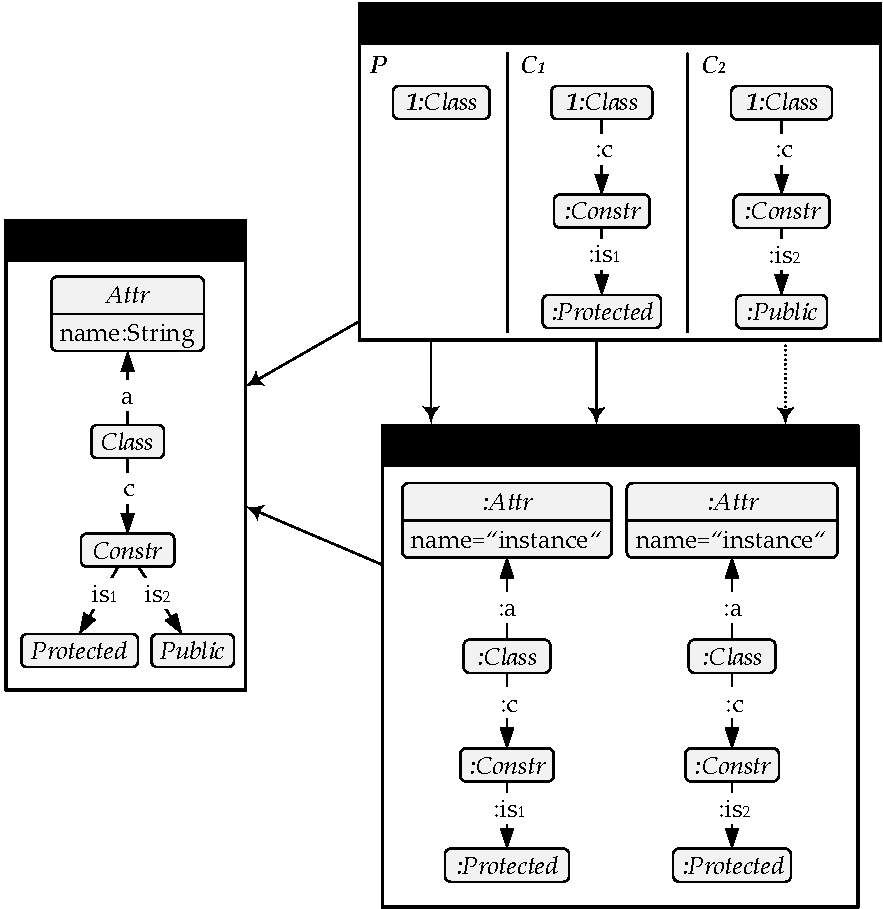
\includegraphics[width=.75\textwidth]{img/gen_intro/conditions.pdf}};
\fill (1.3,5.35) node[inner sep=1pt] (B) {\textcolor{white}{$\vee_{i=(1,2)}(\exists(a_i\colon P \to C_i,\true))$}};
\fill (-5.1,2.7) node[inner sep=1pt] (C) {\textcolor{white}{$\TG$}};
\fill (-.4,.125) node[inner sep=1pt] (D) {\textcolor{white}{$G$}};
\fill (-1.4,1.2) node[inner sep=1pt,fill=white] (E) {$t_P,t_{C_1},t_{C_2}$};
\fill (-.15,1) node[inner sep=1pt,fill=white] (F) {$p$};
\fill (2,1) node[inner sep=1pt,fill=white] (G) {$q_1$};
\fill (4.3,1) node[inner sep=1pt,fill=white] (H) {$q_2$};
\fill (-1.4,-1.1) node[inner sep=1pt,fill=white] (I) {$t_G$};
\end{tikzpicture}
\end{center}
\caption{Graph Constraints and their Satisfaction by Graphs}
\label{fig:sec-gc-gc:conditions}
\end{figure}

\begin{example}[Graph Constraint and Satisfaction]
In reference to the type graph $\TG_\CD$ of UML class diagrams in \cref{sec-gt-graphs,fig:sec-gt-graphs:atg}, \cref{fig:sec-gc-gc:conditions} depicts a modified type graph $\TG$, condition $\ac_P=\vee_{i=(1,2)}(\exists(a\colon P \to C_i,\true))$ over $P$ and graph $G$ both typed over $\TG$ via morphisms $(t_x\colon x \to \TG)_{x \in \{P,C_1,C_2,G\}}$.
According to type graph $\TG$, class diagrams may contain several \code{Class}es, each class may have several \code{Attr}ibutes each with a specific \code{name} of type \code{String} and each class has a \code{Constr}uctor with visibility \code{Protected} or \code{Public}.
Constraint $\ac_P$ claims that each class has a constructor with visibility protected or public.
Graph $G$ both initially and generally satisfies constraint $\ac_P$, since, morphism $p\colon P \to G \in \M$ can be mapped to the left or right class in $G$ such that there exists $q_1\colon C_1 \to G \in \M$ with $q_1 \circ a=p$ and $q_1 \models \true$.
However, there does not exist $q_2\colon C_2 \to G \in \M$ such that $q_2 \circ a=p$.
Thus, for constraint $\ac'_P=\wedge_{i=(1,2)}(\exists(a\colon P \to C_i,\true))$, $G$ satisfies $\ac'_P$ neither initially nor generally.
\envEndMarker
\end{example}

\paragraph*{Visual Notation}
According to \cref{par:sec-gt-graphs:vis}, the mapping of nodes, edges and attributes along morphisms correspond to their naming in visual notation.
For example in \cref{fig:sec-gc-gc:conditions}, node \code{:Class} in $P$ is mapped to node \code{:Class} in $C_1$ ($C_2$) along $a_1$ ($a_2$) as indicated by its name \code{1}.

\begin{figure}[!tb]
\begin{center}
\begin{tikzpicture}[]
\fill (0,0) node[inner sep=1pt] (A) {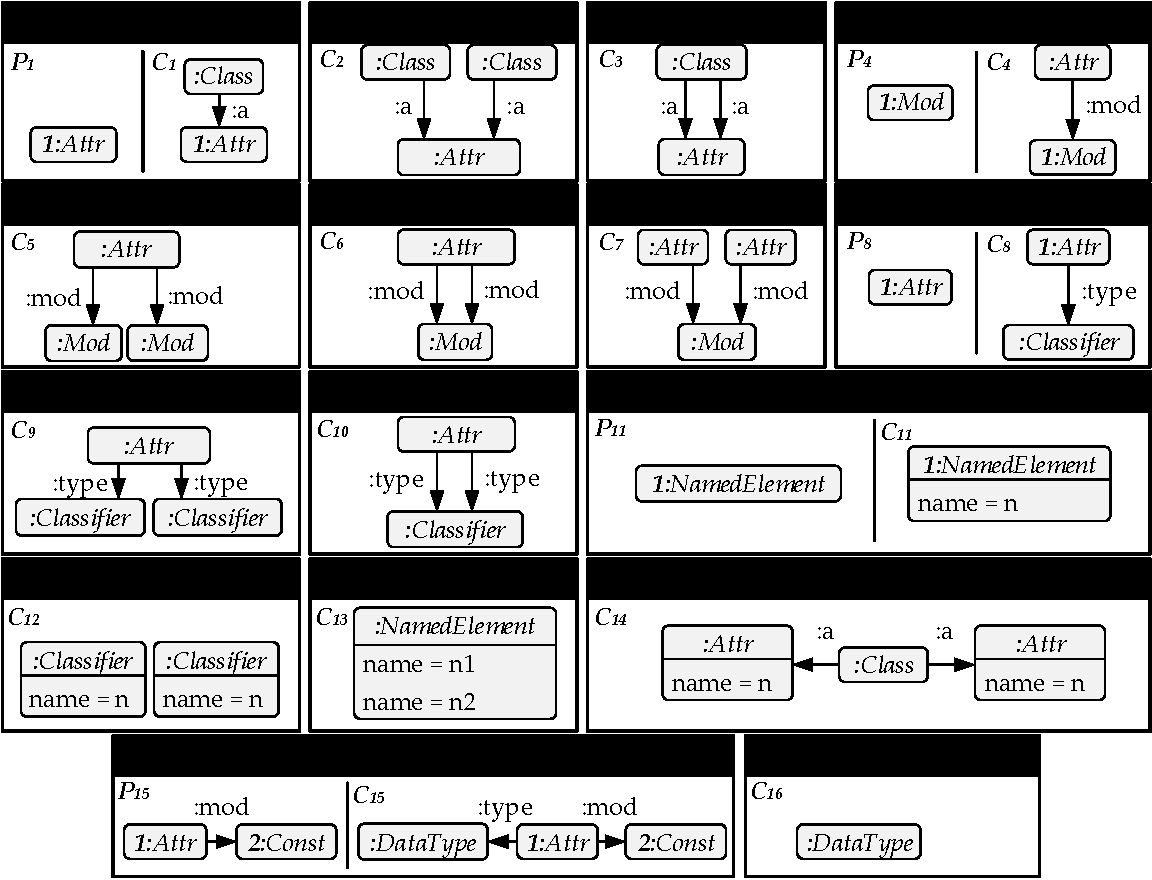
\includegraphics[width=\textwidth]{img/gen_intro/constraints.pdf}};
\fill (-5.8,5.35) node[inner sep=1pt] (B) {\textcolor{white}{$1|\exists(P_1 \to C_1,\true)$}};
\fill (-1.85,5.35) node[inner sep=1pt] (C) {\textcolor{white}{$2|\neg\exists(\varnothing \to C_2,\true)$}};
\fill (1.7,5.35) node[inner sep=1pt] (D) {\textcolor{white}{$3|\neg\exists(\varnothing \to C_3,\true)$}};
\fill (4.9,5.35) node[inner sep=1pt] (E) {\textcolor{white}{$4|\exists(P_4 \to C_4,\true)$}};
\fill (-5.8,3) node[inner sep=1pt] (B2) {\textcolor{white}{$5|\neg\exists(\varnothing \to C_5,\true)$}};
\fill (-1.85,3) node[inner sep=1pt] (C2) {\textcolor{white}{$6|\neg\exists(\varnothing \to C_6,\true)$}};
\fill (1.7,3) node[inner sep=1pt] (D2) {\textcolor{white}{$7|\neg\exists(\varnothing \to C_7,\true)$}};
\fill (4.9,3) node[inner sep=1pt] (E2) {\textcolor{white}{$8|\exists(P_8 \to C_8,\true)$}};
\fill (-5.8,.6) node[inner sep=1pt] (B3) {\textcolor{white}{$9|\neg\exists(\varnothing \to C_9,\true)$}};
\fill (-1.7,.6) node[inner sep=1pt] (C3) {\textcolor{white}{$10|\neg\exists(\varnothing \to C_{10},\true)$}};
\fill (1.85,.6) node[inner sep=1pt] (D3) {\textcolor{white}{$11|\exists(P_{11} \to C_{11},\true)$}};
\fill (-5.7,-1.8) node[inner sep=1pt] (B4) {\textcolor{white}{$12|\neg\exists(\varnothing \to C_{12},\true)$}};
\fill (-1.7,-1.8) node[inner sep=1pt] (C4) {\textcolor{white}{$13|\neg\exists(\varnothing \to C_{13},\true)$}};
\fill (1.85,-1.8) node[inner sep=1pt] (D4) {\textcolor{white}{$14|\neg\exists(\varnothing \to C_{14},\true)$}};
\fill (-4.2,-4.05) node[inner sep=1pt] (C5) {\textcolor{white}{$15|\exists(P_{15} \to C_{15},\true)$}};
\fill (3.75,-4.05) node[inner sep=1pt] (C16) {\textcolor{white}{$16|\exists(\varnothing \to C_{16},\true)$}};
\end{tikzpicture}
\end{center}
\caption{Graph Constraints for UML Class Diagrams}
\label{fig:sec-gc-gc:CD_constraints}
\label{fig:constraints2}
\end{figure}

\begin{example}[Graph Constraints for UML Class Diagrams]
\label{ex:sec-gc-gc:gc_UML_CD}
\cref{fig:sec-gc-gc:CD_constraints} depicts the graph constraints for UML class diagrams over type graph $\TG_\CD$ from \cref{sec-gt-graphs,fig:sec-gt-graphs:atg} which are used for verifying domain completeness in \cref{sec-dc-verification}.
All constraints in \cref{fig:sec-gc-gc:CD_constraints} are designated for general satisfaction.
According to \cref{sec-gt-graphs,ex:sec-gt-graph:type_graph}, this includes the multiplicity constraints in $\TG_\CD$ which complete the meta-model of UML class diagrams:
\begin{enumerate*}
\item Constraint \code{1} claims that each \code{Attr}ibute is assigned to a \code{Class} - in more detail - each attribute is assigned to exactly one class as refined by constraint \code{2},
\item Constraint \code{4} claims that each \code{Mod}ifier is the modifier of some attribute - in more detail - each modifier is the modifier of exactly one attribute as refined by constraint \code{7},
\item Analogously, constraint \code{8} claims that each attribute has some \code{type} - in more detail - each attribute has exactly one type as refined by constraint \code{9}, and
\item Constraint \code{5} claims that each attribute has zero or one modifier.
\end{enumerate*}
Beside the multiplicity constraints, the structure of class diagrams is additionally restricted by the following constraints:
\begin{enumerate*}
\item Constraints \code{3}, \code{6} and \code{10} forbid duplicate edges between two nodes,
\item Constraints \code{11} and \code{13} claim that each \code{NamedElement} has exactly one \code{name},
\item Constraint \code{12} claims that different \code{Classifiers} must have different names,
\item Constraint \code{14} claims that different attributes of the same class must have different names,
\item Constraint \code{15} claims that each \code{Const}ant attribute is of type \code{DataType} and not of type \code{Class}, and
\item Constraint \code{16} claims that there exists at least one \code{DataType}.
\end{enumerate*}
Note that according to \cref{sec-gt-graphs,rem:sec-gt-graphs:inheritance}, abstract node types \code{Mod}, \code{Classifier} and \code{NamedElement} are forbidden to be directly used in graphs like $P_4$.
However, instead of covering abstract types via the formal definition of graphs with node type inheritance, we assume dedicated constraints of the form $\vee_{s \in S}\exists(\code{1:t} \to \code{1:s},\true)$ for each abstract type $\code{t} \in \{\code{Mod},\code{Classifier},\code{NamedElement}\}$ and all non-abstract sub-types $S$ of \code{t} but that are not explicitly depicted in \cref{fig:sec-gc-gc:CD_constraints}.
\envEndMarker
\end{example}

\begin{figure}[!tb]
\begin{center}
\begin{tikzpicture}[]
\fill (0,0) node[inner sep=1pt] (A) {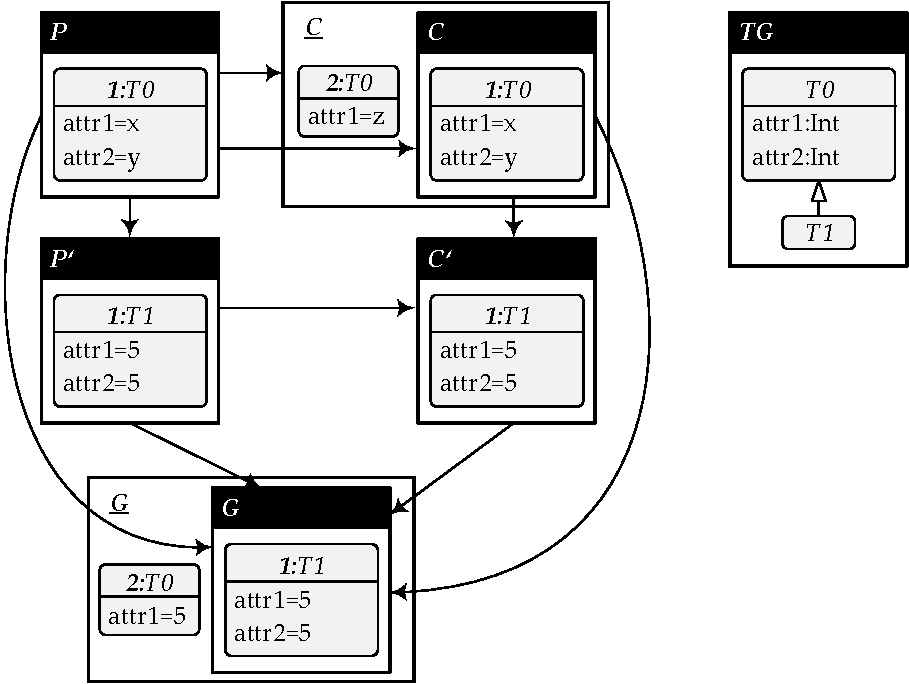
\includegraphics[width=.75\textwidth]{img/gen_intro/ac_schema.pdf}};
\fill (-2.5,2.55) node[inner sep=1pt] (B) {$a$};
\fill (-6.25,0) node[inner sep=1pt] (C) {$p \in \morO$};
\fill (3.2,0) node[inner sep=1pt] (D) {$\not\exists q \in \M$};
\fill (-2.5,.7) node[inner sep=1pt] (E) {$a'$};
\fill (-4.6,1.5) node[inner sep=1pt] (F) {$e \in \E$};
\fill (-4.1,-1.35) node[inner sep=1pt] (G) {$m \in \M$};
\fill (.4,1.5) node[inner sep=1pt] (H) {$e'$};
\fill (-.5,-1.35) node[inner sep=1pt] (I) {$\exists q' \in \M$};
\fill (-2.5,3.5) node[inner sep=1pt] (B2) {$\underline{a}$};
\end{tikzpicture}
\end{center}
\caption{Non-Satisfiability and Instance of Condition $\ac_P=\exists(a\colon P \to C \in \M,\true)$ along $\morO$-matches (left) \& Type Graph $\TG$ (right)}
\label{fig:sec-gc-gc:ac_schema}
\end{figure}

According to \cref{def:condition-satisfaction}, match morphisms $p$ are in $\morO$ but morphisms $q$ are in $\M$ for standard satisfiability of conditions.
Therefore according to \cref{sec-gt-M-adh,rem:sec-gt-M-adh:agraphs_atgi} in $(\AGraphs_\ATGI,\M)$, match morphisms $p$ may be non-injective on the data part $p_D$ and may refine node types along a node type inheritance relation whereas morphisms $q$ are isomorphisms on the data part $q_D$ and are type strict.
More specifically, in category $(\AGraphs_\ATGI,\M)$, conditions $\ac_P$ are often attributed via the $\DSIG$-term algebra $T_\DSIG(X)$ over variables $X$ whereas graphs $G$ are attributed via a concrete $\DSIG$-algebra $D_G$.
In most cases $T_\DSIG(X)$ is not isomorphic to $D_G$, since, different terms in $T_\DSIG(X)$ may be evaluated to the same concrete value in $D_G$, and therefore, $q \in \M$ does not exist.
Thus, a condition $\ac_P$ in $\M$-normal form may be non-satisfiable by $p$ although the condition seems to be a tautology as shown in \cref{fig:sec-gc-gc:ac_schema} where $p$ identifies variables $x$ and $y$ with value $5$ as well as refines type $T_0$ to $T_1$ along the inheritance relation in type graph $\TG$ and there does not exist $q \in \M$ with $q \circ a=p$.
Therefore, according to \cref{def:AC-schemata}, we use the concept of an AC-schema, which interprets a constraint $\ac_P$ as the disjunction of its possible instances $\Inst(\ac_P)$ which may occur in a graph.
Based on the merge construction over extremal $\E$-morphisms w.r.t. $\M$ in \cref{def:merge morphism}, the instances $\Inst(\ac_P)$ subsume all possible type refinements and identifications of data values along match morphisms (cf. \cref{def:sec-gc-gc:cond_inst}).
Since, according to \cref{rem:sec-gc-gc:schemata}, the satisfaction of an AC-schema by match $p \in \morO$ coincides with the satisfaction of the corresponding instance in the schema by $m \in \M$ that is derived by the $\E$-$\M$ factorisation of $p$, this allows us to use AC-schemata as a compact notation and to focus on $\M$-matches while leaving the possible type refinements and identifications of data values implicit.
For example, $(e,\exists(a'\colon P' \to C',\true))$ is an instance of $\ac_P$ in \cref{fig:sec-gc-gc:ac_schema} (the identification of variables $x$ and $y$ as well as the type refinement from $T_0$ to $T_1$ is transferred to the instance), $m \circ e=p$ is an $\E$-$\M$ factorisation of $p$ and furthermore, there exists $q' \in \M$ with $q' \circ a'=m$ (i.e., $m$ satisfies the instance) and therefore, $p$ satisfies the AC-schema of $\ac_P$.
Furthermore, in \cref{th:sec-gc-gc:rel_sat_ac_schema} we show that the standard satisfiability of an AC-schema coincides with the $\morO$-satisfiability of the underlying condition.
This allows an interpretation of conditions via $\morO$-matches and $\morO$-satisfiability from a user point of view while an interpretation via the standard satisfiability of AC-schemata with $\M$-matches is used to prove technical results.

Intuitively, the merge construction transfers the identifications of data values and type refinements along the given morphism $b \colon P \to P'$ to $b' \colon C \to C'$ by respecting the identifications and type refinements along $a\colon P \to C$.
Additionally, it allows for type refinements of elements and identifications of data elements that are in $C$ but not in $P$. 

\begin{definition}[Merge over Morphism (Def. 5.5 in \cite{FAGT2})]
\label{def:merge morphism}
\index{morphism!merge over morphism}
Given a condition $\ac$ over $P$ and a morphism $b: P \rightarrow P'$, then \emph{$\Merge(b,\ac)$ is a condition over $P'$} defined by
\begin{itemize}
\item $\Merge(b,\ac) = \true$ if $\ac = \true$,
\pichskip{5pt}
\parpic[r]{
\begin{tikzpicture}[]
\fill (.5,1.7) node[inner sep=1pt] (P) {$P$};
\fill (2.5,1.7) node[inner sep=1pt] (C) {$C$};
\fill (0.5,-.5) node[inner sep=1pt] (P') {$P'$};
\fill (2.5,-.5) node[inner sep=1pt] (C') {$C'$};
\fill (1.5,.6) node[inner sep=1pt] (N) {$(1)$};
\fill (3.1,1.7) node [isosceles triangle, fill=gray!25,draw,shape border rotate=180,minimum width=0.4cm, inner sep=1pt] (t) {};
\fill (-.1,1.7) node [isosceles triangle, fill=gray!25,draw,minimum width=0.4cm, inner sep=1pt] (t) {};
\fill (-.1,-.5) node [isosceles triangle, fill=gray!25,draw,minimum width=0.4cm, inner sep=1pt] (t) {};
\fill (3.1,-.5) node [isosceles triangle, fill=gray!25,draw,shape border rotate=180,minimum width=0.4cm, inner sep=1pt] (t) {};
\fill (-.5,1.7) node[inner sep=1pt] {$\ac$};
\fill (0.2,-.9) node[inner sep=1pt] {$\Merge(b,\ac)$};
\fill (3.5,1.7) node[inner sep=1pt] {$\ac'$};
\fill (2.7,-.9) node[inner sep=1pt] {$\Merge(b',\ac')$};
%
{
\pgfsetarrowsend{latex}
\draw (P) -> node[above,inner sep=1pt]{$\scriptstyle{a}$} (C);
\draw (P) -> node[left,inner sep=1pt]{$\scriptstyle{b}$} (P');
\pgfsetarrows{right hook-latex}
\draw (P') -> node[above,inner sep=1pt]{$\scriptstyle{a' \in \M}$} (C');
\pgfsetarrows{*-latex}
\draw (C) -> node[right,inner sep=1pt]{$\scriptstyle{b' \in \morO}$} (C');
}
\end{tikzpicture}
}
\item $\Merge(b,\ac) = \vee_{(a',b')\in{\cal F}} \exists(a',\Merge(b',\ac'))$ if $\ac = \exists(a,\ac')$ and ${\cal F} = \{(a',b') \mid a' \in \M \wedge b' \in \morO \wedge (1) \n{ commutes } \wedge (a',b') \n{ are } \n{jointly epimorphic}\}$,
\item $\Merge(b,\ac) = \neg \Merge(b,\ac')$ if $\ac = \neg \ac'$,
\item $\Merge(b,\ac) = \wedge_{i \in{I}} \Merge(b,\ac_i)$ if $\ac = \wedge_{i \in {I}} \ac_i$, or
\end{itemize}
\vspace*{-11pt}
\begin{itemize}
\item $\Merge(b,\ac) = \vee_{i \in{I}} \Merge(b,\ac_i)$ if $\ac = \vee_{i \in {I}} \ac_i$.
\envEndMarker
\end{itemize}
\end{definition}

\begin{remark}
\label{rem:mom}
In $(\AGraphs_\ATGI,\M)$, note that if morphism $a$ identifies elements of $P$ or refines types in $P$ that are not identified or not refined to equal or finer types by morphism $b$, respectively, then $(1)$ cannot be constructed, since, it is required that $a' \in \M$ while $(1)$ commutes, and the merge construction returns $\false$ (an empty disjunction over $(a',b')\in{\cal F}$).
Analogously, if morphism $b$ identifies graph elements of $P$ that are not identified by morphism $a$, then $(1)$ cannot be constructed and $\false$ is returned, since, it is required that $b' \in \morO$ while $(1)$ commutes.
For a characterisation of $\M$- and $\morO$-morphisms in $(\AGraphs_\ATGI,\M)$ we refer to \cref{sec-gt-M-adh,rem:sec-gt-M-adh:agraphs_atgi}.
\envEndMarker
\end{remark}

\begin{definition}[Instances of Conditions]
\label{def:sec-gc-gc:cond_inst}
Given a condition $\ac_P$ over $P$ with $\mor{E}_P = \{e \in \mor{E}\ |\ \dom(e)=P\}$ being the set of all extremal $\E$-morphisms w.r.t. $\M$ with domain $P$.
The \emph{instances of $\ac_P$}\index{graph condition!instance} are given by $\Inst(\ac_P)=\bigcup_{f \in \mor{E}_P}\{(f,\Merge(f,\ac_P))\}$.
Given a set of conditions $C$, then the instances of $C$ are given by $\Inst(C)=\bigcup_{\ac \in C}(\Inst(\ac))$.
\envEndMarker
\end{definition}

\begin{remark}[Instances in $\M$-normal Form]
\label{rem:sec-gc-gc:inst_m_norm_form}
Note that the conditions in instances are in $\M$-normal form by merge construction.
\envEndMarker
\end{remark}

\begin{definition}[AC-schema (Def. 5.6 in \cite{FAGT2})]
\label[definition]{def:AC-schemata}
Given a condition $\ac_P$ over $P$, then \emph{the AC-schema $\ol{\ac}_P$ of $\ac_P$}\index{graph condition!AC-schema} is a condition over $P$ given by  $\ol{\ac}_P = \bigvee_{(f,\ac) \in \Inst(\ac_P)} \exists(f,\ac)$.
For $\ac_P=\true$, $\ol{\ac}_P=\true$.
\envEndMarker
\end{definition}

\vspace*{-10pt}
\pichskip{5pt}
\parpic[r]{
\begin{tikzpicture}[]
\fill (.5,1.3) node[inner sep=1pt] (P) {$P$};
\fill (2,.5) node[inner sep=1pt] (P') {$P'$};
\fill (3.5,1.3) node[inner sep=1pt] (G) {$G$};
\fill (-.1,1.3) node [isosceles triangle, fill=gray!25,draw,minimum width=0.4cm, inner sep=1pt] (t) {};
\fill (1.4,.5) node [isosceles triangle, fill=gray!25,draw,minimum width=0.4cm, inner sep=1pt] (t) {};
\fill (-.6,1.3) node[inner sep=1pt] {$\ol{\ac}_P$};
\fill (.1,0.5) node[inner sep=1pt] {$\Merge(e,\ac_P)$};
%
{
\pgfsetarrows{*-latex}
\draw (P) -> node[above,inner sep=1pt]{$\scriptstyle{p}$} (G);
\pgfsetarrows{->>}
\draw (P) -> node[below left,inner sep=1pt]{$\scriptstyle{e}$} (P');
\pgfsetarrows{right hook-latex}
\draw (P') -> node[below right,inner sep=1pt]{$\scriptstyle{m}$} (G);
}
\end{tikzpicture}}
\vspace*{-10pt}
\begin{remark}[AC-schema satisfaction (Fact 5.8 in \cite{FAGT2})]
\label{rem:sec-gc-gc:schemata}
\index{graph condition!AC-schema!satisfaction}
Given an AC-schema $\ol{\ac}_P$ of condition $\ac_P$ over $P$ and a morphism $p \colon P \to G \in \morO$ with an extremal $\E$-$\M$-factorisation $m \circ e = p$, then $p \models \ol{\ac}_P$ if and only if  $m \models \Merge(e,\ac_P)$ with $(e,\Merge(e,\ac_P)) \in \Inst(\ac_P)$.
Note that the satisfaction of conditions by morphisms in \cref{sec-gt-gc,def:condition-satisfaction} is defined based on $\morO$-morphisms.
However, $m \in \morO$ by $m \in \M$ in $(\AGraphs_\ATGI,\M)$ (cf. \cref{sec-gt-M-adh,rem:sec-gt-M-adh:agraphs_atgi}).
\envEndMarker
\end{remark}

Note that by \cref{def:AC-schemata}, the AC-schema $\ol{\ac}_P$ of a constraint $\ac_P$ over $P$ is again a constraint over $P$.
However, the satisfaction of AC-schemata by objects cannot be directly defined by \cref{rem:sec-gc-gc:init_gen_sat}.
For example, constraint $\neg\ac_P$ in \cref{fig:sec-gc-gc:ac_schema} seems to be a contradiction with $G \not\models \neg\ac_P$ but $G \models \neg\ac_P$ if both algebras of $G$ and $\neg\ac_P$ are not isomorphic, i.e., $p\colon P \to G \in \M$ does not exist (cf. \cref{sec-gt-M-adh,rem:sec-gt-M-adh:agraphs_atgi}).
Therefore, based on \cref{rem:sec-gc-gc:init_gen_sat} the satisfaction of AC-schemata is defined as follows.

\begin{definition}[Initial \& General Satisfaction of AC-schemata]
\label{rem:sec-gc-gc:init_gen_sat_ac_schema}
\index{graph constraint!AC-schema!initial satisfaction}
\index{graph constraint!AC-schema!general satisfaction}
\emph{An object $G$ initially satisfies AC-schema $\ol{\ac}_P$} of constraint $\ac_P$ over $P$, if $\exists p\colon P \to G \in \morO$ such that $p \models \ol{\ac}_P$.
\emph{An object $G$ generally satisfies $\ol{\ac}_P$}, if $\forall p\colon P \to G \in \morO$ it holds that $p \models \ol{\ac}_P$.
By \cref{rem:sec-gc-gc:schemata}, in $\M$-adhesive categories with extremal $\E$-$\M$ factorisations, $G$ initially satisfies $\ol{\ac}_P$ if and only if $\exists$ instance $(e\colon P \to P',\Merge(e,\ac_P)) \in \Inst(\ac_P)$ of $\ac_P$ such that $G \stackrel{I}{\models} \Merge(e,\ac_P)$.
Analogously, $G$ generally satisfies $\ol{\ac}_P$ if and only if $\forall$ instances $(e\colon P \to P',\Merge(e,\ac_P)) \in \Inst(\ac_P)$ it holds that $G \models \Merge(e,\ac_P)$.
For initial and general satisfaction of constraints $\Merge(e,\ac_P)$, we refer to \cref{def:constr_sat,rem:sec-gc-gc:init_gen_sat}.
\envEndMarker
\end{definition}

\begin{remark}[Data in Constraints and Application Conditions]
\label{rem:sec-gc-gc:data_cond}
Consider condition $\ac'_P=\exists(\underline{a}\colon P \to \underline{C},\true)$ in \cref{fig:sec-gc-gc:ac_schema} with $P,\underline{C}$ being attributed graphs and which claims that there is an additional \code{:T0} node with attribute \code{attr1} of value \code{z}.
Assume that $P$ contains a variable \code{z'} in its algebra that is mapped to variable \code{z} in $\underline{C}$ along morphism $\underline{a}$, then the interpretation of $\ac'_P$ according to \cref{rem:sec-gc-gc:init_gen_sat_ac_schema} may be misleading, e.g., in contrast to the intended result, $\underline{G}$ does not generally satisfy the AC-schema $\ol{\ac}'_P$ of constraint $\ac'_P$.
This is due to the fact that the mapping of \code{z} along $\underline{q}\colon \underline{C} \to \underline{G} \in \morO$ is prescribed by the mapping of \code{z'} along match $\underline{p}\colon P \to \underline{G} \in \morO$ in order to obtain $\underline{q} \circ \underline{a}=\underline{p}$ (cf. \cref{th:sec-gc-gc:rel_sat_ac_schema}).
By \cref{rem:sec-gc-gc:init_gen_sat_ac_schema}, for general satisfaction all matches $\underline{p}\colon P \to \underline{G} \in \morO$ are considered, i.e., \code{z'} and therefore also \code{z} may be mapped to the same value than \code{x} or \code{y} (i.e., value \code{5} for the example) but also to any other value along $\underline{p}$ and $\underline{q}$, respectively.
Thus, more precisely, for general satisfaction and graphs $\underline{G}$ that allow different values for variables \code{x}, \code{y} and \code{z}, $\ac'_P$ claims that there are additional \code{:T0} nodes, one with attribute \code{attr1} of value \code{z} that equals to \code{x}, one with attribute \code{attr1} of value \code{z} that equals to \code{y} and one with attribute \code{attr1} of value \code{z} that differs from \code{x} and \code{y}.
The same situation arises for variables that are not used as attribute values in attributed premise and conclusion graphs of conditions but that are non-injectively mapped along the internal morphisms of conditions, since, for matches $\underline{p}$ that are injective on these variables, the corresponding $\underline{q}$-morphism with $\underline{q} \circ \underline{a}=\underline{p}$ does not exist. 
Therefore, for conditions $\ac$ over attributed graphs we generally assume that for all internal morphisms $a\colon P \to C$ in $\ac$ it is true that all variables that are used as attribute values in $C$ but not in $P$ are not in the image of $a$.
Furthermore, all variables in $P$ that are not used as attribute values are injectively mapped along $a$.
Under this general assumption for constraint $\ac'_P$, graph $\underline{G}$ both initially and generally satisfies $\ol{\ac}'_P$.
\envEndMarker
\end{remark}

According to \cref{prop:sec-gc-gc:rel_sat_cond_ac}, for $\M$-matches and the case of category $(\AGraphs_\ATGI,\M)$ (and underlying categories $(\Graphs,\M)$ and $(\Graphs_\TG,\M)$), the interpretation of a condition $\ac_P$ that is type strict via the standard satisfiability of its AC-schema coincides with the standard satisfiability of $\ac_P$ itself.
According to \cref{def:sec-gc-gc:cond_type_strict}, a condition $\ac_P$ over $P$ is type strict, if it is in $\M$-normal form and furthermore, the types of all nodes in conclusions that are not in premise $P$ cannot be refined along morphisms.
Therefore, for $\M$-matches and type strict conditions, the direct interpretation of conditions is equivalent to their interpretation via AC-schemata.
This may not hold for general $\morO$-matches and for conditions that are not type strict.
However, \cref{th:sec-gc-gc:rel_sat_ac_schema} shows for $(\AGraphs_\ATGI,\M)$ and underlying categories that the standard satisfiability of an AC-schema coincides with the $\morO$-satisfiability of the underlying condition.

\begin{definition}[Type Strict Condition]
\label{def:sec-gc-gc:cond_type_strict}
In $(\AGraphs_\ATGI,\M)$, \emph{a condition $\ac_P$ over $P$ is type strict}\index{graph condition!type strict}, if $\ac_P$ is in $\M$-normal form and for all morphisms $a\colon P \to C$ in $\ac_P$ with domain $P$ it holds that for all nodes $n \in V_G^C \setminus a_{G,V_G}(V_G^P)$ that are in $C$ but not in $P$, node type $\type_C(n)$ does not have sub-types in the inheritance relation of type graph $\ATGI$ and therefore, cannot be refined along morphisms.
\envEndMarker
\end{definition}

\begin{proposition}[Relationship between Satisfiability of Conditions and AC-Schemata]
\label{prop:sec-gc-gc:rel_sat_cond_ac}
\index{graph constraint!AC-schema!satisfaction (relationship to conditions I)}
In $(\AGraphs_\ATGI,\M)$, given a type strict condition $\ac_P$ over $P$, its AC-schema $\ol{\ac}_P$ and a match $p:P \to G \in \M$.
Then, $p \models \ac_P$ if and only if $p \models \ol{\ac}_P$.
\envEndMarker
\end{proposition}

\begin{proof}
The proof is presented in \cref{sec-proofs:prop:sec-gc-gc:rel_sat_cond_ac}.
\end{proof}

\begin{proposition}[Relationship between Standard- and $\morO$-Satisfiability of Conditions]
\label{th:sec-gc-gc:rel_sat_ac_schema}
\index{graph constraint!AC-schema!satisfaction (relationship to conditions II)}
In $(\AGraphs_\ATGI,\M)$, given a condition $\ac_P$ over $P$, its AC-schema $\ol{\ac}_P$ and a match $p\colon P \to G \in \morO$.
Then, $p \models_{\morO} \ac_P$ if and only if $p \models \ol{\ac}_P$.
\envEndMarker
\end{proposition}

\begin{proof}
The proof is presented in \cref{sec-proofs:th:sec-gc-gc:rel_sat_ac_schema}.
\end{proof}

\paragraph*{General Assumption}
Note that we interpret conditions by AC-schemata that are formed over (extremal) $\E$-morphisms and their satisfaction can be defined based on (extremal) $\E$-$\M$ factorisations by \cref{rem:sec-gc-gc:schemata}.
Therefore, in addition to the general assumption from \cref{sec-gt-M-adh}, we assume $\M$-adhesive categories with unique (extremal) $\E$-$\M$ factorisation.
Furthermore, we assume that all application conditions and graph constraints are interpreted via their AC-schemata according to \cref{def:AC-schemata}, if not made explicit.
Moreover, we generally assume the assumption from \cref{rem:sec-gc-gc:data_cond} for constraints.

\subsection{Graph Grammars, Transformations \& $\M$-adhesive Transformation Systems}
\label{sec-gt-trafo}
\begin{figure}[!tb]
\begin{center}
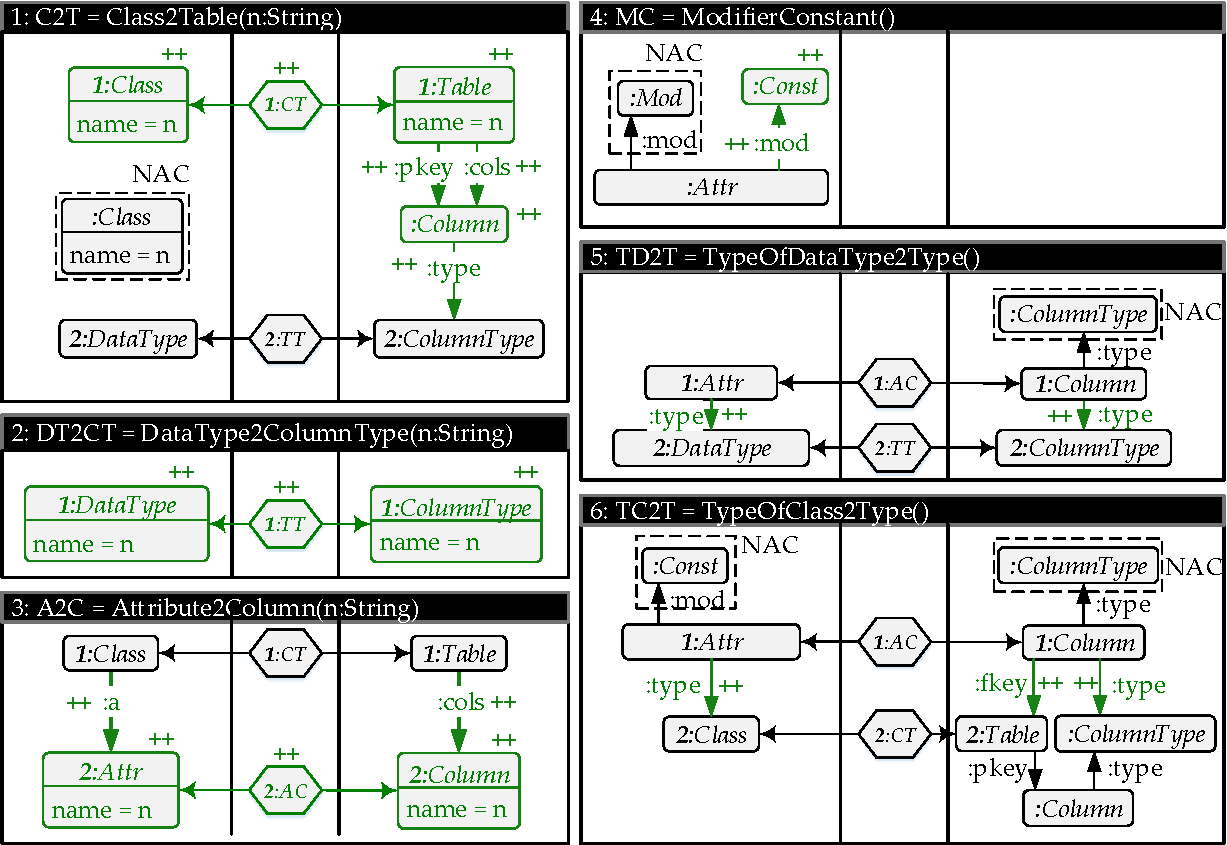
\includegraphics[width=\textwidth]{img/gen_intro/tgg.pdf}
\end{center}
\caption{Triple Graph Grammar (CD2RDBM)}
\label{fig:sec-gt-trafo:tgg}
\label{fig:rules}
\end{figure}

As discussed in \cref{sec-gen-intro-gratrafo}, models are represented by graphs and model transformations and synchronisations are performed based on graph transformations.
Furthermore, graph transformations are performed by applying graph transformation rules to graphs.
According to \cref{def:sec-gt-trafo:rule}, a rule $p$ is a span $p=(L \transB{L} K \trans{r} R)$ of $\M$-morphisms $l$ and $r$ with left-hand side $L$, gluing $K$ and right-hand side $R$.
A rule is applied to a graph $G$ via a match-morphism $m\colon L \to G$ as defined by direct transformations in \cref{def:sec-gt-trafo:trafo}.

\begin{definition}[(Transformation) Rule (Def. 5.12 in \cite{FAGT2})]
\label{def:sec-gt-trafo:rule}
A \emph{plain (transformation) rule $p=(L \transB{l} K \trans{r} R)$}\index{transformation!rule!plain} consists of objects $L,K$ and $R$, called left-hand side, gluing and right-hand side, respectively and two morphisms $l,r \in \M$.
A \emph{(transformation) rule $p=(L \transB{l} K \trans{r} R, \ac_L)$}\index{transformation!rule} consists of a plain rule and a condition $\ac_L$ over $L$, called application condition.\index{application condition}
\envEndMarker
\end{definition}

\parpic[r][r]{
$
\SelectTips{cm}{}
     \xymatrix@R-3.3ex@C-2ex{
     L \ar[dd]|{m} & & K \ar[ll]|{l} \ar[rr]|{r} \ar[dd]|{k} & & R \ar[dd]|{n} \\
     & (1) & & (2) & \\
     G & & D \ar[ll]|{f} \ar[rr]|{g} & & H\\
     }
$
}
\vspace{-1.5ex}
\begin{definition}[Transformation (Def. 5.13 in \cite{FAGT2})]
\label{def:sec-gt-trafo:trafo}
Given a rule $p=(L \transB{l} K \trans{r} R, \ac_L)$, an object $G$, and a morphism $m\colon L \to G$, called match, such that $m \models \ac_L$, \emph{a direct transformation (step) $G \Trans{(p,m)} H$}\index{transformation!direct} from $G$ to an object $H$ via $p$ and match $m$ is given by the pushouts $(1)$ and $(2)$ with co-match $n$\index{match}\index{co-match}.
Given a set of rules $P$, a sequence of direct transformations from $G$ to $H$ via $p \in P$ is called \emph{a transformation (sequence) via $P$}\index{transformation}, written $t\colon G \Trans{*} H$.
\envEndMarker
\end{definition}

Intuitively, the application leads to a graph $H$ where $m(L) \setminus m(l(K))$ is deleted from $G$ and $R \setminus r(K)$ is added while $m(l(K))$ is preserved.
Furthermore, a rule may be equipped with an application condition $\ac_L$ which may restrict the application of the rule to specific matches, i.e, for rule applications, match $m$ must additionally satisfy application condition $\ac_L$.
According to \cref{def:sec-gc-gc:cond_pos}, we distinguish between positive application conditions (PACs) and negative application conditions (NACs)\index{application condition!NAC}\index{application condition!PAC}.
NACs declare forbidden patterns and PACs declare patterns that must exist for rule applications.
We say that a \emph{rule is non-deleting}\index{transformation!rule!non-deleting}, if $l=\id_L$ and $K=L$.
In case of non-deleting rules $p=(L \transB{id} L \xhookrightarrow{r} R,\ac_L)$, we write $p=(L \xhookrightarrow{r} R,\ac_L)$ and pushout $(1)$ in \cref{def:sec-gt-trafo:trafo} is omitted with $D=G$ and $k=m$.
According to \cref{sec-gt-graphs,def:sec-gt-graphs:typed_graphs} and \cref{sec-gt-gc,def:condition-satisfaction}, we say that a rule $p=(L \gets K \to R,\ac_L)$ is typed over type graph $\TG$\index{transformation!rule!typed over}, if $L,K,R$ and $\ac_L$ are typed over common $\TG$.
We take production as synonym for rule\index{production}.

A transformation system is a set of rules.
A transformation system together with a start object constitutes a grammar.
Usually, we take graphs as objects and speak of graph grammars (cf. \cref{sec-gt-M-adh,rem:sec-gt-M-adh}).
The language over a grammar is given by all objects that are reachable from the start object by transformations via the rules of the grammar (cf. \cref{sec-dc-general,def:sec-dc-general:lang}).
We say that a grammar is non-deleting\index{grammar!non-deleting}, if all its rules are non-deleting.
We say that a grammar is typed over $\TG$\index{grammar!typed over}, if the start object and all its rules are typed over $\TG$.
We say that a grammar is without application conditions, if all its rules are plain rules.
A grammar is finite\index{grammar!finite}, if the set of rules is finite.

\begin{definition}[$\M$-adhesive Transformation System \& Grammar]
\label{def:sec-gt-trafo:grammar}
Given an $\M$-adhesive categoriy $(\cat{C},\M)$, \emph{an $\M$-adhesive transformation system $\AS=(P)$}\index{transformation!system} is given by a set of rules $P$.
\emph{A grammar $\GG=(S,\AS)$}\index{grammar} is given by a transformation system $\AS$ and a start object $S$.
\envEndMarker
\end{definition}

\paragraph*{Visual Notation}
\label{par:sec-gt-trafo:vis_not}
In addition to the notational conventions from \cref{par:sec-gt-graphs:vis}, transformation rules are visualised as depicted in \cref{fig:sec-gt-trafo:tgg}.
All graph elements that are marked with \code{++} are added by the rule and therefore, are only contained in the right-hand side of the rule.
All graph elements that are marked with \code{--} are deleted by the rule and therefore, are only contained in the left-hand side of the rule.
All graph elements that are unmarked are preserved by the rule and therefore, are contained in the left-hand side and the gluing of the rule.
Additionally, a rule may be equipped with an application condition which consists of the left-hand side of the rule together with those graph elements that are enclosed by PAC or NAC boxes.

\begin{example}[Rules \& Transformations]
\label{ex:sec-gt-trafo:trafo}
The rules in \cref{fig:sec-gt-trafo:tgg} simultaneously create class diagrams and relational database models.
For each rule $p$, we focus on the projection $p^\SRC$ to the source domain of class diagrams (left parts).
Rule \code{1}$^\SRC$ creates a \code{Class} of \code{name} \code{n} in addition to an existing \code{DataType} but only of there does not already exist a class of the same name (cf. NAC).
Rule \code{2}$^\SRC$ creates a \code{DataType} of \code{name} \code{n}.
Rule \code{3}$^\SRC$ creates an \code{Attribute} of \code{name} \code{n} and assigns it to an existing \code{Class} via edge \code{:a}.
Rule \code{4}$^\SRC$ creates a \code{Const}ant \code{Mod}ifier to an existing attribute but only of the attribute does not already have a modifier (cf. NAC).
Rule \code{5}$^\SRC$ assigns an existing data type to an existing attribute as \code{type}.
Rule \code{6}$^\SRC$ assigns an existing class to an existing attribute as \code{type} but only if the attribute is not \code{Const}ant (cf. NAC).
There is a transformation $\varnothing \Trans{(\code{2}^\SRC,\_)} G_1 \Trans{(\code{1}^\SRC,\_)} G_2 \Trans{(\code{3}^\SRC,\_)} G_3 \Trans{(\code{4}^\SRC,\_)} G_4 \Trans{(\code{5}^\SRC,\_)} \CD$ from the empty graph $\varnothing$ to graph $\CD$ in \cref{sec-gt-graphs,fig:sec-gt-graphs:atg}.
Analogously, we derive six rules by a projection to the right parts that create the elements of relational database models.
\envEndMarker
\end{example}

In view of \cref{sec-dc-general-rec}, we recall the notion of the derived span of transformations.

\begin{definition}[Derived Span \cite{FAGT2}]
\label{def:sec-gt-trafo:derived_span}
Let $t\colon G_0 \Trans{*} G_n$ be a transformation, then the \emph{derived span $\der(t)$ of $t$}\index{transformation!derived span} is inductively defined by
\begin{center}
	$\der(t)=\begin{cases}
	G \transB{\id_G} G \trans{\id_G} G & ,\text{for identical (empty) transformation } t\colon G \Trans{\id} G \\
	G_{i-1} \transB{f_i} D_i \trans{g_i} G_i & ,\text{for }t\colon G_{i-1} \Trans{(p_i,m_i)} G_i \text{ being a direct transformation}\\
	& \text{with pushouts} (1) \text{ and } (2)\\
	G_0 \transB{d'_0 \circ d} D \trans{g_n \circ d_n} G_n & ,\text{for }t\colon G_0 \Trans{*} G_{n-1} \Trans{(p_n,m_m)} G_n \text{ with }\\
	& \der(G_0 \Trans{*} G_{n-1})=(G_0 \transB{d'_0} D' \trans{d'_{n-1}} G_{n-1})\\
	& \text{ and pullback }(PB)
	\end{cases}$
\end{center}
\envEndMarker
\begin{center}
	%\vspace*{.2cm}
	\begin{tikzpicture}[]
	\fill (0,0) node[inner sep=1pt] (G0) {$G_0$};
	\fill (0,0) node[right of=G0,xshift=1cm,inner sep=1pt] (D') {$D'$};
	\fill (0,0) node[right of=D',xshift=1cm,inner sep=1pt] (Gn1) {$G_{n-1}$};
	\fill (0,0) node[right of=Gn1,xshift=1cm,inner sep=1pt] (Dn) {$D_n$};
	\fill (0,0) node[right of=Dn,xshift=1cm,inner sep=1pt] (Gn) {$G_n$};
	\fill (0,0) node[below of=Gn1,yshift=-1cm,inner sep=1pt] (D) {$D$};
	%
	\fill (0,0) node[below of=Gn1,inner sep=1pt] (1) {$(PB)$};
	%
	\fill (0,0) node[left of=G0,xshift=-4cm,inner sep=1pt] (Lp) {$L_i$};
	\fill (0,0) node[right of=Lp,xshift=.5cm,inner sep=1pt] (Kp) {$K_i$};
	\fill (0,0) node[right of=Kp,xshift=.5cm,inner sep=1pt] (Rp) {$R_i$};
	\fill (0,0) node[below of=Lp,yshift=-1cm,inner sep=1pt] (G0p) {$G_{i-1}$};
	\fill (0,0) node[right of=G0p,xshift=.5cm,inner sep=1pt] (D1p) {$D_i$};
	\fill (0,0) node[right of=D1p,xshift=.5cm,inner sep=1pt] (G1p) {$G_i$};
	%
	\fill (0,0) node[left of=Lp,xshift=.3cm,inner sep=1pt] (p1) {$p_i=($};
	\fill (0,0) node[right of=Rp,xshift=-.7cm,inner sep=1pt] (p2) {$)$};
	\fill (0,0) node[right of=Lp,xshift=-.25cm,yshift=-1cm,inner sep=1pt] (1) {$(1)$};
	\fill (0,0) node[right of=Lp,xshift=1.25cm,yshift=-1cm,inner sep=1pt] (2) {$(2)$};
	%
	{
	\pgfsetarrows{right hook-latex}
	%
	\pgfsetarrows{left hook-latex}
	%
	\pgfsetarrows{-latex}
	\path (D') edge[] node[fill=white]{\scriptsize{$d'_0$}} (G0);
	\path (D') edge[] node[fill=white]{\scriptsize{$d'_{n-1}$}} (Gn1);
	\path (Dn) edge[] node[fill=white]{\scriptsize{$f_n$}} (Gn1);
	\path (Dn) edge[] node[fill=white]{\scriptsize{$g_n$}} (Gn);
	\path (D) edge[] node[fill=white]{\scriptsize{$d$}} (D');
	\path (D) edge[] node[fill=white]{\scriptsize{$d_n$}} (Dn);
	%
	\path (Kp) edge[] node[fill=white]{\scriptsize{$l_i$}} (Lp);
	\path (Kp) edge[] node[fill=white]{\scriptsize{$r_i$}} (Rp);
	\path (D1p) edge[] node[fill=white]{\scriptsize{$f_i$}} (G0p);
	\path (D1p) edge[] node[fill=white]{\scriptsize{$g_i$}} (G1p);
	\path (Lp) edge[] node[fill=white]{\scriptsize{$m_i$}} (G0p);
	\path (Kp) edge[] node[]{} (D1p);
	\path (Rp) edge[] node[]{} (G1p);
	%
	\pgfsetarrows{->>}
	%
	}
	\end{tikzpicture}
\end{center}
\end{definition}

\begin{remark}[Derived Span for Non-Deleting Rules]
\label{rem:sec-gc-gc:der_span_non_deleting}
For transformations $t\colon G_0 \Trans{*} G_n$ via non-deleting rules only and with direct transformations $(G_{i-1} \Trans{(p_i,m_i)} G_i)_{i \in \{1,\ldots,n\}}$, the derived span $\der(t)\colon G_0 \to G_n$ of $t$ is given by $\der(t):=g_n \circ \ldots \circ g_1$.
Note that in $\M$-adhesive categories, the derived span for transformations via non-deleting productions is in $\M$ by productions being spans of $\M$-morphisms ($r_i \in \M$), $\M$-morphisms are closed under pushouts, i.e., $g_i \in \M$, and $\M$-composition, i.e., $g_n \circ \ldots \circ g_1 \in \M$.
\envEndMarker
\end{remark}

\parpic[r][r]{
$
\SelectTips{cm}{}
     \xymatrix@R-3.3ex@C-2ex{
     A \ar[dd]|{} \ar[rr]|{} & & B \ar[rr]|{} \ar[dd]|{} & & E \ar[dd]|{} \\
     & (1) & & (2) & \\
     C \ar[rr]|{} & & D \ar[rr]|{} & & F\\
     }
$
}
\vspace{-1.5ex}
We review the following general existing results, as, they are used in definitions or proofs:
\begin{enumerate*}
\item [\textbf{Restriction Theorem} (Thm. 6.18 in \cite{Ehrig:2006:FAG:1121741})]\index{restriction theorem}: Direct transformations can be restricted along specific decompositions of match-morphisms,
\item [\textbf{PO-(De)-Composition} (Lem. A.21 in \cite{Ehrig:2006:FAG:1121741})]\index{pushout!composition}\index{pushout!decomposition}: For pushouts $(1)$ and $(2)$, also $(1)+(2)$ is a pushout, and if $(1)$ and $(1)+(2)$ are pushouts, then also $(2)$, and
\item [\textbf{PB-(De)-Composition} (Lem. A.25 in \cite{Ehrig:2006:FAG:1121741})]\index{pullback!composition}\index{pullback!decomposition}: For pullbacks $(1)$ and $(2)$, also $(1)+(2)$ is a pullback, and if $(2)$ and $(1)+(2)$ are pullbacks, then also $(1)$.
\item [\textbf{Critical Pair}]\index{critical pair}: Given a transformation system $P$, a critical pair $(K_1 \TransB{(p_1,m_1)} O \Trans{(p_2,m_2)} K_2)$ for rules $P$ is a pair of direct transformations $t_1\colon O \Trans{(p_1,m_1)} K_1$ and $t_2\colon O \Trans{(p_2,m_2)} K_2$ with common object $O$ and $p_1,p_2 \in P$ where both transformations are in conflict to each other, intuitively, in the sense that
(1) transformation $t_1$ deletes elements from $O$ to $K_1$ that are ``used'' by match $m_2$ for transformation $t_2$ or vice versa, or
(2) $K_1$ does not satisfy the application condition of $p_2$ anymore or vice versa
and furthermore, where object $O$ is minimal.
Object $O$ is minimal means that matches $m_1$ and $m_2$ are jointly epimorphic (surjective) on $O$, i.e., $O$ only contains elements that are covered by transformations $t_1$ and $t_2$.
In the context of graphs, $O$ is called the conflict graph of the critical pair.\index{conflict graph}
For technical details we refer to Def. 2.39 in \cite{FAGT2}.
Note that we concentrate on critical pairs for rules over graphs with translation (marking) attributes (cf. \cref{sec-mt-tgg,rem:sec-mt-tgg:tr_attr}).
This involves forward translation rules (cf. \cref{sec-mt-tgg,def:sec-mt-tgg:fwd_bwd_tr_rules}), consistency creating rules (cf. \cref{sec-msynch-tgg,def:sec-msynch-tgg:cc_rule}) and marking rules (cf. \cref{sec-dc-verification,def:marking-rule}) that only update translation (marking) attributes from $\False$ to $\True$ while preserving the remaining graph structure in terms of deletions.
Note that technically, the update of an attribute is a deletion of the old attribute value followed by a creation of the new attribute value (cf. \cref{sec-gt-graphs,def:sec-gt-graphs:agraphs}).
\cref{fig:sec-gt-trafo:cp} depicts a critical pair $(K_1 \TransB{(m(4^S),m_1)} O \Trans{(m(4^S),m_2)} K_2)$ for marking rule $m(4^S)$ of rule $4^S$ in \cref{ex:sec-gt-trafo:trafo}.
Both transformations simultaneously update the marking attribute of node \code{1:Const} from $\False$ to $\True$.
\item [\textbf{Strict Confluence}]\index{critical pair!strict confluence}: A critical pair $(K_1 \TransB{(p_1,m_1)} O \Trans{(p_2,m_2)} K_2)$ is strictly confluent, if there are transformations $t_1\colon K_1 \Trans{*} O'$ and $t_2\colon K_2 \Trans{*} O'$ to common $O'$ such that all elements that are preserved by both transformations of the critical pair are also preserved by transformations $t_1$ and $t_2$ such that they can be embedded into bigger contexts.
For technical details we refer to Def. 2.42 in \cite{FAGT2}.
\item [\textbf{Local Confluence Theorem} (Thm. 2.43 in \cite{FAGT2})]\index{local confluence}\index{local confluence theorem}: A transformation system $P$ is locally confluent if, for all direct transformations $G \Trans{(p_1,m_1)} H_1$ and $G \Trans{(p_2,m_2)} H_2$ via $p_1,p_2 \in P$, there is an object $X$ and transformations $H_1 \Trans{*} X$ and $H_" \Trans{*} X$ via $P$.
A transformation system is locally confluent if all its critical pairs are strictly confluent.
\item [\textbf{Confluence} (Lem. 3.32 in \cite{Ehrig:2006:FAG:1121741})]\index{confluence}: A transformation system $P$ is confluent if, for all transformations $G \Trans{*} H_1$ and $G \Trans{*} H_2$ via $P$, there is an object $X$ and transformations $H_1 \Trans{*} X$ and $H_2 \Trans{*} X$ via $P$.
Every terminating and locally confluent transformation system is also confluent.
\index{transformation!system!terminating}A transformation system $P$ is terminating if there is no infinite transformation sequence via $P$.
\end{enumerate*}

\begin{figure}[!tb]
\begin{center}
	\begin{tikzpicture}[]
	\fill (0,0) node[inner sep=1pt] (P) {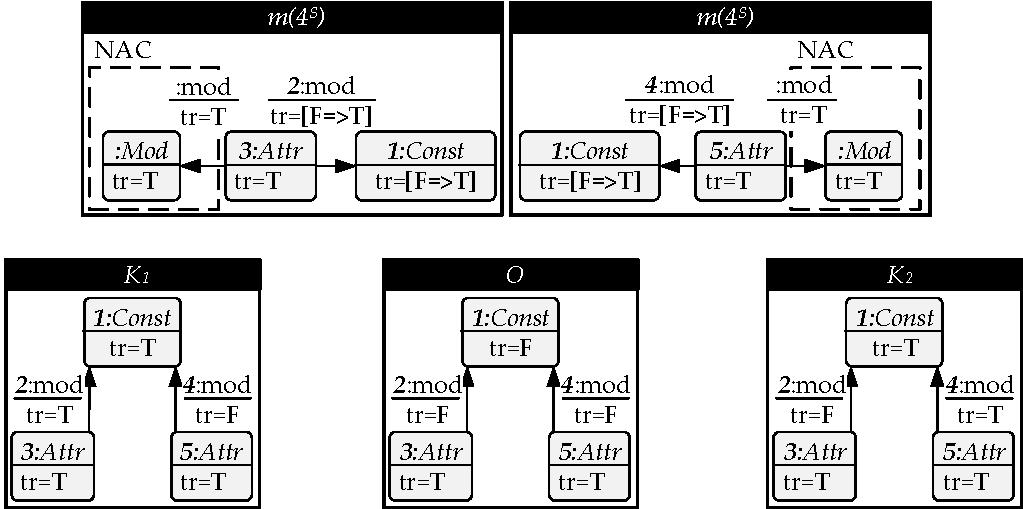
\includegraphics[width=.95\textwidth]{img/dc/cp.pdf}};
	\fill (-1,.7) node[] (A) {};
	\fill (-1,-.2) node[] (B) {};
	\fill (1,.7) node[] (A2) {};
	\fill (1,-.2) node[] (B2) {};
	\fill (-2,-1.5) node[] (C) {};
	\fill (-3.5,-1.5) node[] (D) {};
	\fill (2,-1.5) node[] (C2) {};
	\fill (3.5,-1.5) node[] (D2) {};
	{
	\pgfsetarrows{-latex}
	\path (A) edge[] node[left]{\scriptsize{$m_1$}} (B);
	\path (A2) edge[] node[right]{\scriptsize{$m_2$}} (B2);
	\pgfsetarrows{->}
	\path (C) edge[double distance = 2.5pt, inner sep=8pt] node[above]{\scriptsize{$(m(4^S),m_1)$}} (D);
	\path (C2) edge[double distance = 2.5pt, inner sep=8pt] node[above]{\scriptsize{$(m(4^S),m_2)$}} (D2);
	}
	\end{tikzpicture}
\end{center}
\caption{Critical Pair $(K_1 \TransB{(m(4^S),m_1)} O \Trans{(m(4^S),m_2)} K_2)$}
\label{fig:sec-gt-trafo:cp}
\end{figure}

\paragraph*{General Assumption}
For $(\AGraphs_\ATGI,\M)$ and underlying categories, we restrict the application of rules to almost injective matches $m \in \morO$ (cf. \cref{sec-gt-M-adh,rem:sec-gt-M-adh:agraphs_atgi}).
Furthermore, we assume that all application conditions are interpreted via their AC-schemata according to \cref{sec-gt-gc,def:AC-schemata}.
Moreover, we generally assume the assumption from \cref{sec-gt-gc,rem:sec-gc-gc:data_cond} for application conditions.


\section{Model Transformation \& Synchronisation based on TGGs}
\label{sec-gen-intro-mt-ms-tgg}

This section reviews the concept of triple graph grammars (TGGs) as well as model transformations and synchronisations based on TGGs.

\subsection{Triple Graphs \& Triple Graph Grammars (TGGs)}
\label{sec-tgg}
According to \cref{sec-gen-intro-mt}, triple graph grammars (TGGs) allow the definition of visual, declarative transformation specifications for model transformations and synchronisations.
Therefore, we review basic notions of TGGs from \cite{FAGT2}.

A triple graph\index{triple graph} $G=(G^\SRC \transB{s_G} G^\C \trans{t_G} G^\T)$ is an integrated model consisting of a source graph $G^\SRC$, a target graph $G^\T$ and explicit correspondences between them (cf. Def. 3.3 in \cite{FAGT2}).
The correspondences are given by correspondence graph $G^\C$ together with morphisms $s_G\colon G^\C \to G^\SRC$ and $t_G\colon G^\C \to G^\T$ specifying a correspondence relation between elements of $G^\SRC$ and elements of $G^\T$.
Triple graphs $G$ and $H$ are related by triple graph morphisms\index{triple graph!morphism} $m=(m^\SRC,m^\C,m^\T) : G \rightarrow H$~\cite{DBLP:conf/wg/Schurr94,DBLP:conf/fase/EhrigEEHT07} consisting of three morphisms $m^\SRC\colon G^\SRC \to H^\SRC,m^\C\colon G^\C \to H^\C$ and $m^\T\colon G^\T \to H^\T$ that preserve the associated correspondences, i.e., $m^\SRC \circ s_G=s_H \circ m^\C$ and $m^\T \circ t_G=t_H \circ m^\C$.  
Therefore, analogously to attributed graphs and morphisms in \cref{sec-gt-graphs,def:sec-gt-graphs:agraphs}, an attributed triple graph $G=(G^\SRC \transB{s_G} G^\C \trans{t_G} G^\T)$ is defined by attributed graphs $G^\SRC,G^C,G^\T$ and attributed graph morphisms $s_G,t_G$.
An attributed triple graph morphism $f=(f^\SRC,f^\C,f^\T)\colon G \rightarrow H$ between two attributed triple graphs $G$ and $H$ is defined by three attributed graph morphisms $f^\SRC,f^\C,f^\T$.
Furthermore, analogously to typed attributed graphs and morphisms (with node type inheritance) in \cref{sec-gt-graphs,def:sec-gt-graphs:typed_attr_graphs,rem:sec-gt-graphs:inheritance}, a typed attributed triple graph\index{triple graph!typed \& attributed} over attributed triple graph $\TG$ as attributed triple type graph is defined by an attributed triple graph $G$ together with an attributed triple graph morphism $\type_G\colon G \to \TG$.
A typed attributed triple graph morphism\index{triple graph!morphism!typed \& attributed} $f\colon G \rightarrow H$ between typed attributed triple graphs $G$ and $H$ is an attributed triple graph morphism $f$ such that $(\type_H^X \circ f^X=\type_G^X)_{X \in \{\SRC,\C,\T\}}$.
The category $(\ATrGraphs_\ATGI,\M)$\index{category!$\ATrGraphs_\ATGI$} of all typed attributed triple graphs over triple type graph $\ATGI$ and all typed attributed triple graph morphisms with node type inheritance is $\M$-adhesive where according to \cref{sec-gt-M-adh,rem:sec-gt-M-adh:agraphs_atgi}, triple graph $\M$-($\morO$-)morphisms\index{category!$\ATrGraphs_\ATGI$!$\M$-morphisms}\index{category!$\ATrGraphs_\ATGI$!$\morO$-morphisms} are componentwise $\M$-($\morO$-) morphisms in $(\AGraphs_\ATGI,\M)$ (cf. Def. 3.4 \& Thm. 7.2 in \cite{FAGT2}).
Analogously to the definition of rules in \cref{sec-gt-trafo,def:sec-gt-trafo:rule} and according to \cite{GEH11} and Def. 3.8 in \cite{FAGT2}, a triple rule\index{triple rule} $\tr=(\ol{\tr}\colon L \xhookrightarrow{} R,\ac_L)$ is given by a triple graph $\M$-morphism $\ol{tr}$ and an application condition $\ac_L$ over $L$.
Thus, triple rules are non-deleting and specify how a given consistently integrated model (triple graph) can be extended simultaneously on all three components source, correspondence and target yielding again a consistently integrated model. 
Analogously to (direct) transformations in \cref{sec-gt-trafo,def:sec-gt-trafo:trafo}, for a given triple graph $G$, triple rule $\tr=(\ol{\tr}\colon L \xhookrightarrow{} R,\ac_L)$ and triple graph match-morphism $m\colon L \to G$ with $m \models \ac_L$, (direct) triple graph transformations\index{triple graph!transformation}\index{triple graph!transformation!direct} $G \Trans{(\tr,m)} H$ via $\tr$ and $m$ are defined (cf. Def. 3.8 in \cite{FAGT2}).
Analogously to grammars in \cref{sec-gt-trafo,def:sec-gt-trafo:grammar}, a triple graph grammar $\TGG=(S,\TR)$\index{triple graph!grammar (TGG)} consists of a triple start graph $S$ and a set $\TR$ of triple rules, and generates the triple graph language of consistently integrated models $\Lang(\TGG)=\{G \mid \exists \text{ triple graph transformation } S \Trans{*} G \text{ via }\TR\}$\index{triple graph!grammar (TGG)!language $\Lang(\TGG)$} with consistent source and target languages $\Lang(\TGG)^\SRC=\{G^\SRC \mid (G^\SRC \leftarrow G^\C \to G^\T) \in \Lang(\TGG) \}$ and $\Lang(\TGG)^\T=\{G^\T \mid (G^\SRC \leftarrow G^\C \to G^\T) \in \Lang(\TGG) \}$\index{triple graph!grammar (TGG)!language $\Lang(\TGG)^\SRC$}\index{triple graph!grammar (TGG)!language $\Lang(\TGG)^\T$} (cf. Def. 3.12 in \cite{FAGT2}).

\paragraph*{Visual Notation}
As depicted in \cref{sec-gt-trafo,fig:sec-gt-trafo:tgg}, the three components of triple graphs are visualised in three separate boxes.
According to the conventions for the visual notation of graphs in \cref{par:sec-gt-graphs:vis}, the mapping of graph elements along correspondence morphisms $s_G$ and $t_G$ of triple graphs $G$ correspond to their naming in visual notation.
Additionally, the conventions for the visual notation of rules in \cref{par:sec-gt-trafo:vis_not} are also used for triple rules.
For example, each triple rule in \cref{sec-gt-trafo,fig:sec-gt-trafo:tgg} visualises the different domains of UML class diagrams (left boxes), correspondences (boxes inbetween) and relational database models (right boxes) in separate boxes.
Furthermore, each rule adds those graph elements that are marked with \code{++} while all unmarked elements are preserved when being applied.
Moreover, for example in rule \code{3} node \code{1:CT} is mapped to nodes \code{1:Class} and \code{1:Table} along the correspondence morphisms, respectively.

\begin{example}[Triple Graph, Triple Type Graph \& Triple Graph Grammar (CD2RDBM)]
\label{ex:sec-tgg:tg}
Attributed triple graph $G=(\CD \transB{s} C \trans{t} \RDBM)$ in \cref{sec-gt-graphs,fig:sec-gt-graphs:atg} is typed over attributed triple type graph $\TG=(\TG_\CD \gets \TG_C \to \TG_\RDBM)$ via attributed triple graph type morphism $(\type_\CD,\type_C,\type_\RDBM)\colon G \to \TG$.
According to the type graph, each \code{Attr}ibute in CDs correspond to a \code{Column} in RDBMs via a node of type \code{AC}, each \code{Class} in CDs correspond to a \code{Table} in RDBMs via a node of type \code{CT}, and each \code{DataType} in CDs correspond to a \code{ColumnType} in RDBMs via a node of type \code{TT}.
Therefore, node \code{1:DataType} in source graph $\CD$ corresponds to node \code{1:ColumnType} in target graph $\RDBM$ via node \code{1:TT} in correspondence graph $C$, node \code{2:Attr} in $\CD$ corresponds to node \code{1:Column} in $\RDBM$ via node \code{2:AC} in $C$, and node \code{4:Class} in $\CD$ corresponds to node \code{4:Table} in $\RDBM$ via node \code{4:CT} in $C$.
\cref{sec-gt-trafo,fig:sec-gt-trafo:tgg} depicts the triple rules for creating consistently integrated models of UML class diagrams (CDs) together with corresponding relational database models (RDBMs).
The rules are all typed over $\TG$.
Given a triple graph with class diagram $\CD'$ in the source and database model $\RDBM'$ in the target such that $\CD'$ contains a \code{DataType} with corresponding \code{ColumnType} in $\RDBM'$, then the application of triple rule \code{1} extends the triple graph simultaneously on all three components in the sense that it simultaneously adds a \code{Class} to $\CD'$ together with a corresponding \code{Table} to $\RDBM'$ both of \code{name} \code{n} but only if $\CD'$ does not already contain a class of the same name (cf. NAC).
Furthermore, the table is equipped with a dedicated \code{Column} as primary key (\code{pkey}) of \code{type} \code{ColumnType}.
Rule \code{2} simultaneously adds a \code{DataType} to CDs together with a corresponding \code{ColumnType} to RDBMs, both of \code{name} \code{n}.
Rule \code{3} simultaneously adds an \code{Attr}ibute to CDs together with a corresponding \code{Column} to RDBMs, both of \code{name} \code{n}, and assigns both to an existing class in CDs and the corresponding table in RDBMs.
Rule \code{4} adds a \code{Const}ant modifier to an existing attribute in CDs but only if the attribute does not already have a modifier (cf. NAC).
Rule \code{5} simultaneously assigns an existing data type to an existing attribute as type in CDs and the corresponding column type to the corresponding column as type in RDBMs but only if the column does not already have a type (cf. NAC).
Rule \code{6} simultaneously assigns an existing class to an existing attribute as type in CDs and the corresponding table to the corresponding column as foreign key (\code{fkey}) in RDBMs but only if the column does not already have a type (cf. NAC), i.e., the type of the primary key column (\code{pkey}) of the table is additionally assigned to the column as type.
The TGG $CD2RDBM=(\varnothing,\{\code{1},\code{2},\code{3},\code{4},\code{5},\code{6}\})$ for transforming CDs into RDBMs is given by the empty triple start graph $\varnothing$ together with triple rules \code{1} to \code{6}, i.e., the TGG is typed over $\TG$.
Triple graph $G=(\CD \transB{s} C \trans{t} \RDBM)$ in \cref{sec-gt-graphs,fig:sec-gt-graphs:atg} can be obtained via direct triple graph transformations $\varnothing \Trans{(\code{2},\_)} G_1 \Trans{(\code{1},\_)} G_2 \Trans{(\code{3},\_)} G_3 \Trans{(\code{4},\_)} G_4 \Trans{(\code{5},\_)} G$ via triple rules $\code{1}$ to $\code{5}$, i.e., $G \in \Lang(CD2RDBM),\CD \in \Lang(CD2RDBM)^\SRC$ and $\RDBM \in \Lang(CD2RDBM)^\T$.
\envEndMarker
\end{example}

\begin{remark}[Meta-Modelling \& Model Transformation]
As discussed in \cref{sec-gen-intro-mt}, a model transformation between DSLs $\Lang(D_1)$ and $\Lang(D_2)$ transforms models from language $\Lang(D_1)$ in source domain $D_1$ to language $\Lang(D_2)$ in target domain $D_2$ where each DSL is defined by a meta-model in the corresponding domain.
In the given context of graph transformations, a meta-model is defined by a type graph together with a set of graph constraints.
Therefore, a DSL $\Lang(D)$ in domain $D$ is given by all graphs that are typed over the domain type graph and that satisfy the domain constraints (cf. \cref{sec-dc-general,def:sec-dc-general:lang}).
The attributed triple type graph $\TG=(\TG_\CD \gets \TG_C \to \TG_\RDBM)$ in \cref{sec-gt-graphs,fig:sec-gt-graphs:atg} contains both the type graph $\TG_\CD$ for the domain of class diagrams (CDs) and type graph $\TG_\RDBM$ for the domain of relational database models (RDBMs) together with type graph $\TG_C$ for correspondences between both.
Additionally, \cref{sec-gt-gc,fig:sec-gc-gc:CD_constraints} represents the graph constraints for the domain of CDs (constraints for RDBMs can be defined analogously).
Thus, for the model transformation CD2RDBM from CDs to RDBMs and in view of \cref{sec-gen-intro-mt,fig:sec-gen-intro-msynch:mt_msynch} (a) and (c), a graph $M$ ($M'$) conforms to the meta-model in domain CD (RDBM), if $M$ ($M'$) is typed over $\TG_\CD$ ($\TG_\RDBM$) and satisfies the CD (RDBM) constraints.
Graph $\CD$ in \cref{fig:sec-gt-graphs:atg} conforms to the CD meta-model and graph $\RDBM$ conforms to the RDBM meta-model.
The transformation language of CD2RDBM is given by the formalism of TGGs and contains all TGGs that conform to the meta-models in domains CD and RDBM, i.e., all TGGs that are typed over triple type graph $\TG$ and that satisfy the domain constraints.
According to \cref{ex:sec-tgg:tg}, the TGG CD2RDBM in \cref{sec-gt-trafo,fig:sec-gt-trafo:tgg} is in (conforms to) the transformation language of CD2RDBM and therefore, is a valid transformation specification.
Transformation CD2RDBM may take graph $\CD$ in \cref{fig:sec-gt-graphs:atg} as input and outputs triple graph $(\CD \transB{s} C \trans{t} \RDBM)$ with correspondences $C$ if being executed based on the TGG in \cref{fig:sec-gt-trafo:tgg}.
In \cref{sec-mt-tgg,def:sec-mt-tgg:mt_ft}, we review the execution of transformations based on model transformation sequences and a given TGG in more detail.
\envEndMarker
\end{remark}


\subsection{Model Transformations based on TGGs}
\label{sec-mt-tgg}
A model transformation $\MT\colon \Lang(D_1) \TransMT \Lang(D_2)$ is specified by a TGG (cf. \cref{sec-gen-intro-mt}).
In the following we review the existing concept of executing model transformations from \cite{FAGT2} based on model transformation sequences via operational rules of a given TGG, called forward translation triple rules.
According to \cref{def:sec-mt-tgg:fwd_bwd_tr_rules}, the operational forward translation rules of a given TGG are derived from the set of triple rules of the TGG by an automatic construction \cite{DBLP:conf/gg/SchurrK08,Hermann:2010:EAE:1866272.1866277}.
For each triple rule $\tr$, the construction yields a corresponding forward translation triple rule $\tr_\FT$ which is identical to $\tr$ on the correspondence and target components, i.e., $\tr_\FT$ creates the same graph elements as $\tr$ in the correspondence and target parts.
For the source part, $\tr_\FT$ does not create elements but already contains the created source elements of $\tr$ in the left-hand side.
Each source graph element in $\tr_\FT$ is equipped with a translation attribute with attribute value false ($\False$ - not yet transformed) for those elements that are created by $\tr$ and attribute value true ($\True$ - has been already transformed) for all other elements (cf. \cref{rem:sec-mt-tgg:tr_attr}).
Therefore, the application of a forward translation rule $\tr_\FT$ is the transformation of all source elements that are marked with $\False$ to corresponding target elements.
Furthermore, rule $\tr_\FT$ updates all translation attribute values from $\False$ to $\True$ in order to mark that the corresponding elements has been transformed.
According to \cref{def:sec-mt-tgg:mt_ft}, a forward model transformation is executed by applying operational forward translation rules successively in so called model transformation sequences.
Thus, the execution of a model transformation corresponds to the abstract description in \cref{sec-gen-intro-gratrafo} where the update of the translation attribute values from $\False$ to $\True$ corresponds to the marking of graph elements to keep track of the elements that already have been transformed during the execution.
The backward case of transforming models from $\Lang(D_1)$ in source domain $D_1$ to $\Lang(D_2)$ in target domain $D_2$ via backward translation rules is defined analogously and omitted in the following.
For technical details we refer to Chapter 7 in \cite{FAGT2}.

The extension of rules with translation attributes from \cref{rem:sec-mt-tgg:tr_attr} is used for the definition of forward translation rules in \cref{def:sec-mt-tgg:fwd_bwd_tr_rules} and for the definition of marking rules in \cref{sec-dc-verification} that are part of verifying domain completeness.

\begin{remark}[Graphs with Translation Attributes]
\label{rem:sec-mt-tgg:tr_attr}
Given an attributed graph $\AG=(G,D)$ and a subset $M \subseteq G$ of its elements (nodes, edges or attributes), we call \emph{$\AG'$ a graph with translation attributes over $\AG$}\index{graph!with translation attributes} if it extends $\AG$ by one Boolean-valued translation attribute for each element in $M$.
The translation attribute for a node or edge is specified by an attribute $\tr$.
The translation attribute for an attribute $a$ of a node or edge is specified by an attribute $\tr\_a$.
With $\AG \oplus \Att^\True_M$ we denote the graph with translation attributes over $\AG$ which extends $\AG$ by a translation attribute for each element in $M \subseteq G$, and all these translation attributes are set to $\True$.
Similarly, $\AG \oplus Att^\False_M$ denotes adding to $\AG$ all these translation attributes, but this time they are set to $\False$.
With $\Att^x(\AG),x \in \{\False,\True\}$ we denote $\AG \oplus \Att^x_G$.
For technical details we refer to Sec. 7.4.1 in \cite{FAGT2}.
\envEndMarker
\end{remark}

According to \cref{def:sec-mt-tgg:T-Ext}, for forward translation rules with application conditions $\ac$, each element in $\ac$ that is not in the premise of $\ac$ also need to be extended by a translation attribute of value $\True$.
For triple rules, $X$ restricts the extension to elements of specific triple components (source, correspondence and target).

\begin{definition}[$\True$-Extension of Application Conditions (Def. 7.28 in \cite{FAGT2})]
\label{def:sec-mt-tgg:T-Ext}
\index{application condition!$\True$-Extension}
Given an application condition $\ac_P$ over premise graph $P$, a graph $P'$ with translation attributes over $P$ and a subset of triple components $X \subseteq \{S,C,T\}$, then the $\True$-extension $tExt(\ac_P,P',X)$ of $\ac_P$ is inductively defined by:
\begin{itemize}
  \item $\tExt(\true,P',X)=\true$
  \item $\tExt(\exists(a=(\inc_P,a_D)\colon P \to C, \ac_C),P',X)=\exists(a_E\colon P' \to C',\tExt(\ac_C,C',X))$ with
  \begin{enumerate}
    \item $C'=P' +_P C \oplus \cup_{x \in X}(\Att^\True_{C^x\setminus P^x})$, and
    \item $a_E=(\inc'_P,a_D)$ with algebra homomorphism $a_D$ on the data part and inclusion $\inc'_P$ on the graph part as derived from $\inc_P$.
  \end{enumerate}
\item $\tExt(\neg(\ac'_P),P',X)=\neg(\tExt(\ac'_P,P',X))$
  \item $\tExt(\ac_{P,1} \wedge \ac_{P,2},P',X)=\tExt(\ac_{P,1},P',X) \wedge \tExt(\ac_{P,2},P',X)$
  \item $\tExt(\ac_{P,1} \vee \ac_{P,2},P',X)=\tExt(\ac_{P,1},P',X) \vee \tExt(\ac_{P,2},P',X)$
  \envEndMarker
\end{itemize}
\end{definition}

According to \cite{FAGT2}, for model transformations and synchronisations, we restrict the application conditions of triple rules to $S$-consistent application conditions.

\begin{remark}[$S$-consistent Application Conditions]
\label{rem:sec-mt-tgg:s_consistent}
According to Def. 7.8 in \cite{FAGT2}, an application condition $\ac_P$ is source consistent ($S$-consistent)\index{application condition!$S$-consistent}, if it can be decomposed into a semantically equivalent conjunction $\ac_P \equiv \ac_S \wedge \ac_F$ such that $\ac_S$ does restrict the source component only and $\ac_F$ does restrict the correspondence and target components only, i.e., relations of restricting elements between the correspondence and source parts in $\ac_P$ may be problematic.
All application conditions in running examples of this thesis are $S$-consistent.
\envEndMarker
\end{remark}

Forward translation rules are used in \cref{def:sec-mt-tgg:mt_ft} for executing model transformations and in \cref{sec-dom-compl-mt,thm:sec-dom-compl-mt-without-acs} for verifying the domain completeness of model transformations.

\begin{definition}[Forward Translation Rule (Def. 7.29 in \cite{FAGT2})]
\label{def:sec-mt-tgg:fwd_bwd_tr_rules}
Given a triple rule $\tr=((\tr^\SRC,\tr^\C,\tr^\T)\colon L=(L^\SRC \transB{s_L} L^\C \trans{t_L} L^\T) \to R=(R^\SRC \transB{s_R} R^\C \trans{t_R} R^\T),\ac_L)$ with $S$-consistent application condition $\ac_L$ over $L$, then \emph{the forward translation rule $\tr_\FT$ of $\tr$}\index{triple rule!forward translation rule} is given by $\tr_\FT=(L_\FT \transB{l_\FT} K_\FT \trans{r_\FT} R_\FT,\ac_\FT)$ with:
\begin{enumerate*}
  \item $L_\FT=(R^\SRC \transB{\tr^\SRC \circ s_L} L^\C \trans{t_L} L^\T) \oplus \Att^\True_{(\tr^\SRC(L^\SRC) \gets \varnothing \to \varnothing)} \oplus \Att^\False_{(R^\SRC \gets \varnothing \to \varnothing) \setminus (\tr^\SRC(L^\SRC) \gets \varnothing \to \varnothing)}$,
  \item $K_\FT=(R^\SRC \transB{\tr^\SRC \circ s_L} L^\C \trans{t_L} L^\T) \oplus \Att^\True_{(\tr^\SRC(L^\SRC) \gets \varnothing \to \varnothing)}$,
  \item $R_\FT=(R^\SRC \transB{s_R} R^\C \trans{t_R} R^\T) \oplus \Att^\True_{(R^\SRC \gets \varnothing \to \varnothing)}$,
  \item $l_\FT$ and $r_\FT$ are the induced inclusions, and
  \item $\ac_\FT=\tExt(\ac_L,L_\FT,\{S\})$.
\end{enumerate*}
With $\TR_\FT$ we denote the set of forward translation rules $\tr_\FT$ of all triple rules $\tr \in \TR$ for a given set of triple rules $\TR$.
\envEndMarker
\end{definition}

\begin{definition}[Complete Forward Translation Sequence (Def. 7.33 in \cite{FAGT2})]
\label{def:sec-mt-tgg:compl_ft}
A forward translation sequence $G_0 \Trans{\tr^*_{\FT}} G_n$ via $\TR_\FT$ with almost injective matches is \emph{complete}\index{model transformation!forward translation sequence}, if no further forward translation rule is applicable and all translation attributes in $G_n$ are set to $\True$.
\envEndMarker
\end{definition}

\begin{definition}[Model Transformation based on Forward Translation Rules (Def. 7.34 in \cite{FAGT2})]
\label{def:sec-mt-tgg:mt_ft}
Given a triple type graph $\TG=(\TG^\SRC \gets \TG^\C \to \TG^\T)$ and a set $\TR$ of triple rules typed over $\TG$, then a \emph{model transformation sequence}\index{model transformation!sequence} $(G^S,G'_0 \Trans{\tr^*_{\FT}} G'_n,G^T)$ based on forward translation rules $\TR_{\FT}$ from a source graph $G^S$ in the source domain to a target graph $G^T$ in the target domain consists of a complete forward translation sequence $G'_0 \Trans{\tr^*_{\FT}} G'_n$ typed over $\TG'=\TG \oplus \Att^\False_{(\TG^S \gets \varnothing \to \varnothing)} \oplus \Att^\True_{(\TG^S \gets \varnothing \to \varnothing)}$ based on $\TR_{\FT}$ with $G'_0=(\Att^\False(G^S) \gets \varnothing \to \varnothing)$ and $G'_n=(\Att^\True(G^S) \gets G^C \to G^T)$.
A \emph{model transformation}\index{model transformation} $\MT\colon \Lang(\TG^S) \TransMT \Lang(\TG^T)$ based on $\TR_{\FT}$ is defined by all model transformation sequences as above with $G^S \in \Lang(\TG^S)$ and $G^T \in \Lang(\TG^T)$ (cf. \cref{sec-dc-general,def:sec-dc-general:lang} for $\Lang(\TG^\SRC)$ and $\Lang(\TG^\T)$).
\envEndMarker
\end{definition}

\begin{figure}[!tb]
\begin{center}
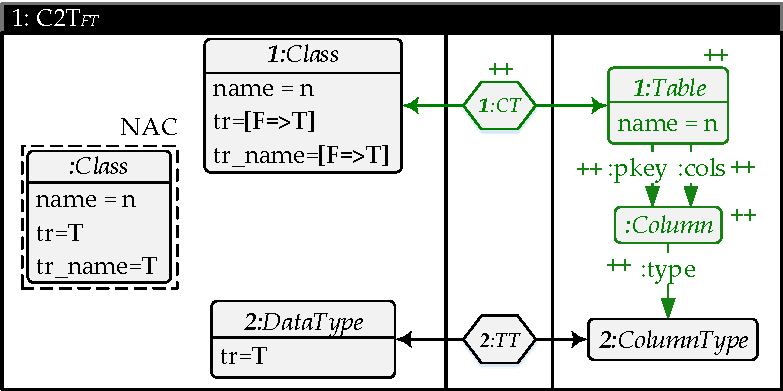
\includegraphics[width=.7\textwidth]{img/gen_intro/ft.pdf}
\end{center}
\caption{Forward Translation Rule}
\label{fig:sec-mt-tgg:fwd_tr_rule}
\end{figure}

\begin{example}[Forward Translation Rule \& Model Transformation]
\label{ex:sec-mt-tgg:fwd_mt}
Rule \code{C2T}$_\FT$ in \cref{fig:sec-mt-tgg:fwd_tr_rule} is the forward translation rule of triple rule \code{C2T} in \cref{sec-gt-trafo,fig:sec-gt-trafo:tgg}.
Node \code{1:Class} and attribute \code{name} are created by rule \code{C2T} in the source and therefore, are initially marked with translation attribute $\False$ and updated to $\True$ in rule \code{C2T}$_\FT$, denoted by $[\False => \True]$.
All other source and NAC elements of \code{C2T} are initially marked with $\True$ in \code{C2T}$_\FT$ and remain unchanged.
Furthermore, the correspondence and target components of \code{C2T}$_\FT$ are identical to those of rule \code{C2T}.
Note that a forward translation rule does also contain the application condition of the target component but without any markings if existent in the underlying triple rule as it is the case for triple rules \code{TD2T} and \code{TC2T}.
Graph $\CD$ in \cref{sec-gt-graphs,fig:sec-gt-graphs:atg} can be transformed to graph $\RDBM$ via model transformation sequence $(\CD,G'_0 \Trans{\code{DT2CT}_\FT(``INT'')} G'_1 \Trans{\code{C2T}_\FT(``Person'')} G'_2 \Trans{\code{A2C}_\FT(``DOB'')} G'_3 \Trans{\code{MC}_\FT} G'_4 \Trans{\code{TD2T}_\FT} G'_5,\RDBM)$ based on the forward translation rules of the triple rules in \cref{sec-gt-trafo,fig:sec-gt-trafo:tgg} with integrated model $G'_5=(\Att^\True(\CD) \gets G^\C \to \RDBM)$.
The model transformation CD2RDBM is given by all corresponding model transformation sequences based on the forward translation rules of the triple rules in \cref{sec-gt-trafo,fig:sec-gt-trafo:tgg}.
\envEndMarker
\end{example}

\paragraph*{General Assumption}
\label{rem:sec-mt-tgg:gen_ass}
Note that the definition of forward translation rules is based on attributions in attributed graphs (cf. \cref{rem:sec-mt-tgg:tr_attr,def:sec-mt-tgg:fwd_bwd_tr_rules}).
Therefore, we assume category $(\ATrGraphs_\ATGI,\M)$ for model transformations and synchronisations.
According to the general assumption for model transformations based on TGGs in Sec. 7.1 in \cite{FAGT2} and analogously to the general assumption for rule applications in \cref{sec-gt-trafo}, we assume that triple rules are applied based on transformations via almost injective matches $m \in \morO$ and where all internal morphisms of application conditions are almost injective (cf. \cref{sec-tgg} for $\morO$-morphisms in $(\ATrGraphs_\ATGI,\M)$).
In the context of model transformations and synchronisations, we generally assume the empty triple graph $\varnothing$ as start graph for TGGs and that all application conditions of triple rules are $S$-consistent.


\subsection{Model Synchronisations based on TGGs}
\label{sec-msynch-tgg}
\begin{figure}[!tb]
\begin{center}
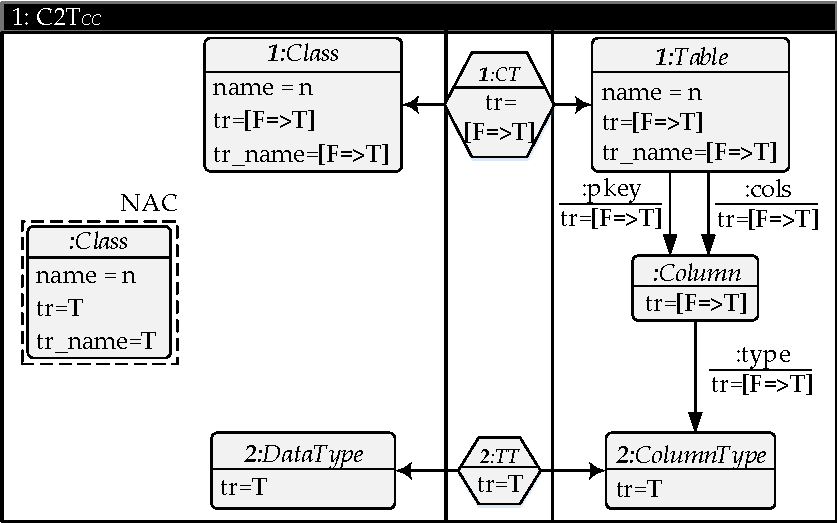
\includegraphics[width=.75\textwidth]{img/gen_intro/cc.pdf}
\end{center}
\caption{Consistency Creating Rule}
\label{fig:sec-msynch-tgg:cc_rule}
\end{figure}

Given a triple type graph $\TG=(\TG^\SRC \gets \TG^\C \to \TG^\T)$ with source domain $\Lang(\TG^\SRC)$ and target domain $\Lang(\TG^T)$ (cf. \cref{sec-dc-general,def:sec-dc-general:lang} for $\Lang(\TG^\SRC)$ and $\Lang(\TG^\T)$).
A source (target) model update\index{model update} $\delta$ on source graph $G \in \Lang(\TG^\SRC)$ (target graph $G \in \Lang(\TG^\T)$) is a span of inclusions $\delta=(G \transB{u_1} H \trans{u_2} G'),u_1,u_2 \in \M$ with $G,H,G' \in \Lang(\TG^\SRC)$ ($G,H,G' \in \Lang(\TG^\T)$).
Elements $G \setminus u_1(H)$ are deleted in $G$ whereas elements $G' \setminus u_2(H)$ are added to $G$.
With $\Delta^\SRC$ ($\Delta^\T$) we denote the set of all source (target) model updates.
A model synchronisation is a propagation of model updates from the source to the target domain via forward propagation operation $\fPpg$.
\index{model synchronisation}Operation $\fPpg$ takes a triple graph $(G^\SRC \gets G^\C \to G^\T)$ typed over $\TG$ together with a source model update $\delta^\SRC=(G^\SRC \gets H^\SRC \to G'^\SRC) \in \Delta^\SRC$ on $G^\SRC$ as input and outputs a target model update $\delta^\T=(G^\T \gets H^\T \to G'^\T) \in \Delta^\T$ on $G^\T$ together with a triple graph $(G'^\SRC \gets G'^\C \to G'^\T)$ typed over $\TG$ that interrelates the results $G'^\SRC$ and $G'^\T$ of both updates via correspondence $G'^\C$.
This corresponds to the informal description of model synchronisations in \cref{sec-gen-intro-msynch}.
The backward case of propagating updates from the target to the source domain via backward propagation operation $\bPpg$ is defined analogously and omitted in the following.
According to Def. 9.18 in \cite{FAGT2}, the synchronisation operation $\fPpg$ is a composition of three auxiliary operations $\fAln,\del$ and $\fAdd$.
For technical details we refer to Chapter 9 in \cite{FAGT2}.
Operation $\del$ relies on operational consistency creating (CC) rules \cite{DBLP:journals/sosym/0001EOCDXGE15}.
Similarly to forward translation rules in \cref{sec-mt-tgg,def:sec-mt-tgg:fwd_bwd_tr_rules}, the CC rule $\tr_\CC$ of a given triple rule $\tr$ does not create elements in the sense that it already contains all elements of $\tr$ including the created elements in the left-hand side and furthermore, each element that is created by $\tr$ is initially marked with translation attribute $\False$ und updated to $\True$, written $[\False => \True]$, while all other elements are initially marked with $\True$ and remain unchanged.
Rule \code{C2T}$_\CC$ in \cref{fig:sec-msynch-tgg:cc_rule} is the CC rule of triple rule \code{C2T} in \cref{sec-gt-trafo,fig:sec-gt-trafo:tgg}.
For CC rules we review the existing result in \cref{fact:sec-msynch-tgg:equ_tr_cc} which is used to prove \cref{sec-dc-verification,lem:equivalence-marking-emptySG}.

\begin{definition}[Consistency Creating (CC) Rule (Def. 7.44 in \cite{FAGT2})]
\label{def:sec-msynch-tgg:cc_rule}
\index{triple rule!consistency creating rule}
Given a triple rule $\tr=(L \to R,\ac_L)$, then \emph{the consistency creating rule $\tr_\CC$ of $\tr$} is given by $\tr_\CC=(L_\CC \transB{l_\CC} K_\CC \trans{r_\CC} R_\CC,\ac_\CC)$ with:
\begin{enumerate*}
  \item $L_\CC=(R \oplus \Att^\True_L \oplus \Att^\False_{R \setminus L})$,
  \item $K_\CC=(R \oplus \Att^\True_L)$,
  \item $R_\CC=(R \oplus \Att^\True_L \oplus \Att^\True_{R \setminus L})$,
  \item $l_\CC$ and $r_\CC$ are the induced inclusions, and
  \item $\ac_\CC=\tExt(\ac_L,L_\CC,\{S,C,T\})$.
\end{enumerate*}
With $\TR_\CC$ we denote the set of consistency creating rules $\tr_\CC$ of all triple rules $\tr \in \TR$ for a given set of triple rules $\TR$.
\envEndMarker
\end{definition}

\begin{figure}[!tb]
\begin{center}
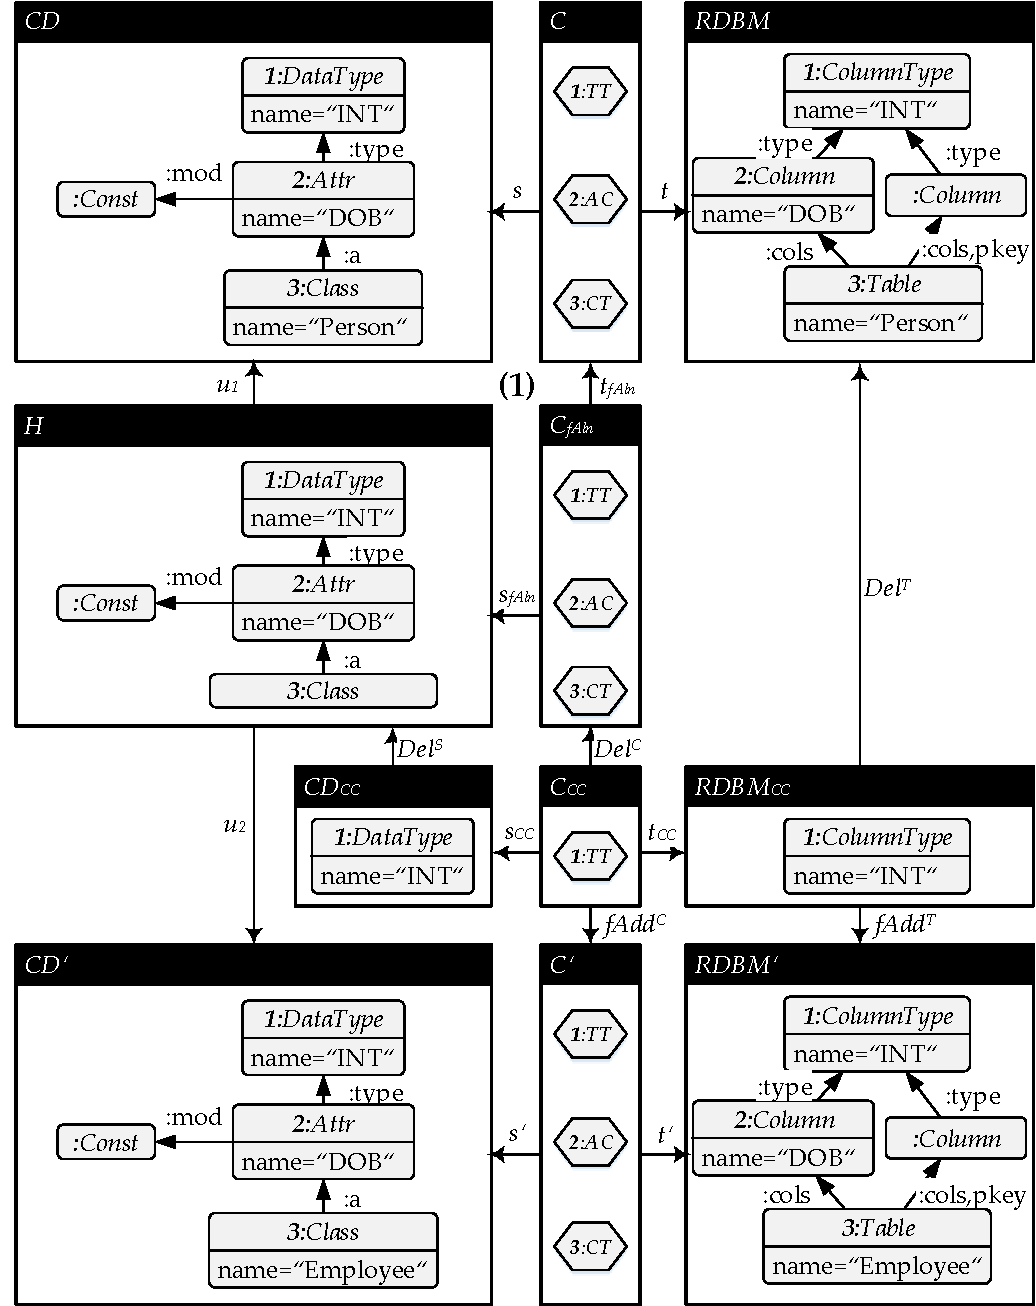
\includegraphics[width=.85\textwidth]{img/gen_intro/sync.pdf}
\end{center}
\caption{Model Synchronisation via Forward Propagation Operation $\fPpg$}
\label{fig:sec-msynch-tgg:fwd}
\end{figure}

\begin{remark}[Meta-Modelling \& Model Synchronisation]
Given the triple type graph $\TG=(\TG_\CD \gets \TG_C \to \TG_\RDBM)$ from \cref{fig:sec-gt-graphs:atg} with triple graph $G=(\CD \gets C \to \RDBM) \in \Lang(\TG)$ and source model update $\delta=(\CD \transB{u_1} H \trans{u_2} \CD')$ in \cref{fig:sec-msynch-tgg:fwd}, then $\fPpg(G,\delta)=(G',\delta')$ with $G'=(\CD' \transB{s'} C' \trans{t'} \RDBM') \in \Lang(\TG)$ and target model update $\delta'=(\RDBM \transB{\del^\T} \RDBM_\CC \trans{\fAdd^\T} \RDBM')$.
Target update $\delta'$ on $\RDBM$ reflects the change of source update $\delta$ on $\CD$ (the \code{name} of the \code{Class} is changed from \code{Person} to \code{Employee}) in the target domain.
The output $(G',\delta')$ is obtained by three sequential operations $\fAln,\del$ and $\fAdd$:
Alignment operation $\fAln$ creates pullback $(1)$ in order to align deletions of update $\delta$ to the correspondence component and yields triple graph $G_1=(H \transB{s_\fAln} C_\fAln \trans{t \circ t_\fAln} \RDBM)$.
Operation $\del$ creates the maximal consistently integrated triple sub-graph of $G_1$ by creating the graph $\Att^\False(G_1)$ with translation attributes over $G_1$ and applying CC rules $\TR_\CC$ as long as possible afterwards.
The maximal consistently integrated sub-graph is given by all $\True$-marked elements, i.e., by triple graph $G_2=(\CD_\CC \transB{s_\CC} C_\CC \trans{t_\CC} \RDBM_\CC)$ with inclusion $(\del^\SRC,\del^\C,\del^\T)\colon G_2 \to G_1$ (the translation attributes are omitted in \cref{fig:sec-msynch-tgg:fwd}).
Operation $\fAdd$ adds those elements to $G_2$ that are created by update $\delta$ leading to triple graph $G_3=(\CD' \transB{u_2 \circ \del^\SRC \circ s_\CC} C_\CC \trans{t_\CC} \RDBM_\CC)$ where additionally all elements that are creatd by $\delta$ are marked with translation attributes $\False$.
Finally, a complete forward translation sequence $G_3 \Trans{\tr^*_\FT} G'$ leads to output $(G',\delta')$.
\envEndMarker
\end{remark}

\begin{fact}[Equivalence of Triple and Extended Consistency Creating Sequences (Fact 10 in \cite{heocdx11})]
\label{fact:sec-msynch-tgg:equ_tr_cc}
Let $\TGG=(\varnothing,\TR)$ be a triple graph grammar typed over triple type graph $\ATGI$ with empty start graph $\varnothing$ and derived consistency creating rules $\TR_\CC$ of triple rules $\TR$.
Let $G \in \Lang(\ATGI)$ be a graph according to \cref{sec-dc-general,def:sec-dc-general:lang}, then the following are equivalent for almost injective matches $m \in \morO$.
\begin{itemize}
	\item There exists a consistency creating sequence $\Att^\False(G) \Trans{\tr_\CC^*} G \oplus \Att_{G_k}^\True \oplus \Att_{G \setminus G_k}^\False$ via consistency creating rules $\TR_\CC$.% with intermediate steps $(G'_i \Trans{(m_i,m(p_i))} G'_{i+1})$, where $m(p_i)=(L_i \xhookleftarrow{} K_i \xhookrightarrow{} R_i)$ and $\quotient{m_i}{L_i^{\False}}$ is type strict
	\item There exists a triple graph transformation $\varnothing \Trans{\tr^*} G_k$ via $\TR$ with injective embedding $f\colon G_k \to G$.% with intermediate steps $G_i \Trans{(m_i,p_i)} G_{i+1}$.
\envEndMarker
\end{itemize}
\end{fact}

\paragraph*{General Assumption}
Note that the definition of CC rules is based on attributions in attributed graphs.
Therefore, we assume all general assumptions from \cref{rem:sec-mt-tgg:gen_ass}. 

\section[Properties of Model Transformations \& Synchronisations]{Properties of Model Transformations \& Synchronisations (``Classical" Completeness \& Correctness)}
\label{sec-gen-intro-compl}
Model transformations and synchronisations based on TGGs share the following important properties:
\begin{enumerate*}
\item efficiency,
\item TGGs allow intuitive and maintainable tranformation specifications with sufficient expressiveness,
\item bidirectionality,
\item type consistency,
\item termination,
\item functional behaviour (termination + confluence), and
\item information preservation (cf. Sec. 3.1 in \cite{FAGT2}).
\end{enumerate*}
% \begin{enumerate}
%   \item \textbf{Consistency:} For a model transformation (synchronisation) from models of (model updates in) a source DSL $\Lang^S$ into models of (model updates in) a target DSL $\Lang^T$, the model transformation specification have to be in accordance with the meta-models of languages $\Lang^S$ and $\Lang^T$ such that the specification can be executed on the set of source models (model updates) (cf. \cref{sec-gen-intro-mt}).
%   In the formal setting of model transformations based on TGGs in \cref{sec-mt-tgg}, this property holds by definition.
%   \item \textbf{Termination:} For each source model (model update) as input, the transformation (synchronisation) terminates with some output.
%   According to Def. 7.34 in \cite{FAGT2}, a model transformation in the sense of \cref{def:sec-mt-tgg:mt_ft} is \emph{terminating}, if there are no infinite forward translation sequences starting with $G'_0=(\Att^\False(G^S) \gets \varnothing \to \varnothing)$ for some source graph $G^S$ in the source domain.
%   As forward translation sequences changes the values of translation attributes of elements from $\False$ to $\True$ at each step, for finite inputs and non-trivial translation rules it is ensured that the transformation and synchronisation terminates (cf. Fact 8.13 in \cite{FAGT2}).
%   \item \textbf{Confluence:} For each source model (model update) as input, if the transformation (synchronisation) terminates with some output, then the output is unique (up to isomorphism), i.e., the transformation (synchronisation) always leads to the same result for a given input.
%   Global confluence of the transformation (synchronisation) can be verified by verifying strict confluence of critical pairs w.r.t. the given TGG (cf. Thm. 8.29 in \cite{FAGT2}).
%   \item \textbf{Functional Behaviour:} Functional behaviour combines the criterions of termination and confluence - For each source model (model update) as input, the transformation (synchronisation) terminates and returns a unique result.
%   \item \textbf{Information Preservation:} For a model transformation from source to target domain, this transformation is also used from target to source such that for each forward transformation starting at source model $G^S$ the backward transformation leads to $G^S$ again and vice versa.
%   Therefore, the transformation covers information in the source domain only that are also contained in the target domain and vice versa.
%   For technical details we refer to Def. 8.35 in \cite{FAGT2} and \cite{DBLP:conf/fase/EhrigEEHT07}.
%   For model synchronisations the concept of information preservation over both domains is expressed by the (weak) invertability property of model synchronisations (cf. Fig. 9.5 in \cite{FAGT2}).
%   \item \textbf{Syntactical Correctness:} For each input in the source domain the model transformation (synchronisation) has to lead an outpout that conforms to the meta-model of the target domain.
%   \item \textbf{Semantic Correctness:} The semantics of the source input model has to be preserved or reflected by the semantics of the resulting target model of the model transformation (synchronisation).
%   \item \textbf{Syntactical Completeness:} The model transformation (synchronisation) can be applied on each model (model update) of the source domain.
% \end{enumerate}
Two further essential properties for the results in \cref{sec-dom-compl-mt,sec-dom-compl-mt-synch} are syntactical correctness and completeness referred to as ``classical" correctness and completeness to not confuse with domain completeness.
Syntactical correctness means that for each input in the source domain, if the model transformation (synchronisation) leads to an output, then the output conforms to the meta-model of the target domain.
Syntactical completeness means that the model transformation (synchronisation) can be applied on each model (model update) in the source domain.

\begin{definition}[``Classical" Syntactical Correctness and Completeness of Model Transformations (Def. 8.3 in \cite{FAGT2})]
\label{def:sec-gen-intro-compl:classical_corr_compl_mt}
\index{model transformation!''classical'' syntactical correctness}
\index{model transformation!''classical'' syntactical completeness}
A model transformation $\MT\colon \Lang(\TG^S) \TransMT \Lang(\TG^T)$ based on forward rules is
\begin{enumerate}
  \item \emph{syntactically correct} if for each model transformation sequence $(G^S,G_0 \Trans{\tr^*_F} G_n,G^T)$ there is $G \in \Lang(\TGG)$ with $G=(G^S \gets G^C \to G^T)$ implying further that $G^S \in \Lang(\TGG)^S$ and $G^T \in \Lang(\TGG)^T$, and it is
  \item \emph{syntactically complete} if for each $G^S \in \Lang(\TGG)^S$ there is $G=(G^S \gets G^C \to G^T) \in \Lang(\TGG)$ with a model transformation sequence $(G^S,G_0 \Trans{\tr^*_F} G_n,G^T)$ and $G_n=G$.
  The backward direction is defined analogously.
  \envEndMarker
\end{enumerate}
\end{definition}

\begin{definition}[``Classical" Syntactical Correctness and Completeness of Model Synchronisations (Fig. 9.5 in \cite{FAGT2})]
\index{model synchronisation!''classical'' syntactical correctness}
\index{model synchronisation!''classical'' syntactical completeness}
A forward model synchronisation via $\fPpg$ is
\begin{enumerate}
  \item \emph{syntactically correct} if for all consistently integrated models $M=(M^\SRC \gets M^\C \to M^\T) \in \Lang(\TGG)$ and source model updates $u\colon M^\SRC \gets H^\SRC \to M'^\SRC,u' \in \Delta^S,M'^\SRC \in \Lang(\TGG)^\SRC$ it holds that $\fPpg(M,\id^S)=(M,\id^T)$ and $\fPpg(M,u)=(M',u')$ such that $M'=(M'^\SRC \gets M'^\C \to M'^\T)$ and $M' \in \Lang(\TGG)$, if $\fPpg$ yields a result, and it is
  \item \emph{syntactically complete} if $\fPpg$ can be applied on each input integrated models $M \in \Lang(\TGG)$ and source model updates $u \in \Delta^S$ and it always yields a result for any valid input.
  \envEndMarker
\end{enumerate}
\end{definition}

\begin{remark}[``Classical" Syntactical Correctness and Completeness]
\label{rem:sec-gen-intro-compl:classical_corr_compl_mt}
According to Thm. 8.4 and Cor. 8.5 in \cite{FAGT2}, each model transformation $\MT$ based on forward (translation) rules is ``classically" syntactically correct and complete.
For forward translation rules, each model transformation sequence $(G^S,G_0 \Trans{\tr^*_F} G_n,G^T)$ based on forward rules in \cref{def:sec-gen-intro-compl:classical_corr_compl_mt} is substituted by a corresponding model transformation sequence $(G^S,G'_0 \Trans{\tr^*_\FT} G'_n,G^T)$ based on forward translation rules.
According to Thm. 9.25 in \cite{FAGT2}, $\fPpg$ is syntactically correct and complete for kernel-grounded and deterministic sets of operational rules $\TR_\CC$ and $\TR_\FT$.
\envEndMarker
\end{remark}


\chapter{Domain Completeness}
\label{sec-dom-compl}

In \cref{sec-dc-general}, we introduce the domain completeness problem and show its undecidability in $(\cat{\Graphs_\TG},\M)$ and derivative categories of graphs with finite restrictions to the graphs, underlying type graph $\TG$, grammar, constraints and application conditions.
Intuitively, the fact that the domain completeness problem is undecidable means that it is impossible to construct a single algorithm which completely solves the problem in the sense that the algorithm terminates and returns the correct yes-or-no answer concerning $\Lang(C) \subseteq \Lang(\GG)$ for each input $\Lang(C)$ and $\Lang(\GG)$.
This led to the development of sufficient conditions that can be checked by a procedure for verifying domain completeness in $(\cat{AGraphs_\ATGI},\M)$ and underlying categories.
It is guaranteed that the procedure terminates under certain assumptions.
Note that the conditions are sufficient only without being necessary, i.e., the proposed verification technique is an under-approximation approach for solving the domain completeness problem in the sense that the approach does not yield false positives but may yield false negatives.
Thus, if the conditions are fulfilled, then domain completeness holds but if the conditions are not fulfilled, then domain completeness does not necessarily not hold but may also hold.
Therefore, we can give a concrete answer only to a subset of all constraint-grammar pairs for which domain completeness holds.

\cref{sec-dc-verification} presents the verification technique.
\cref{sec-dc-general-lim} presents the limitations of the approach.
\cref{sec-dc-general-rec,sec-dc-general-res} presents various extensions of the approach.
\cref{sec-dc-general-rec} introduces the notion of recursive constraints for enabling the verification of domain completeness in view of infinite constraints which describe recursive graph patterns.
% \cref{sec-dc-general-gen} presents the generation of domain constraints from graph grammars such that domain completeness automatically holds for the derived constraints.
% This can be used if the domain constraints are unknown or for checking against an existing set of domain constraints.
Finally, in \cref{sec-dc-general-res} we consider the verification of domain completeness under restrictions of the domain type graph.
This reflects the situation where only a subset of all constituents of the given domain is subjected to the verification.

\section{Domain Completeness Problem \& Undecidability}
\label{sec-dc-general}
We assume that the constituents of a domain are given by a type graph whereas valid sentences in that domain are additionally restricted by a set of graph constraints.
Thus, valid sentences in a domain are expressed by typed graphs as domain models that satisfy the given domain constraints.
The domain-specific language (DSL) is given by all valid sentences in that domain, i.e., by all graphs typed over the domain type graph and that satisfy the domain constraints.

\begin{definition}[(Domain-Specific) Languages over Graph Constraints, Grammars \& Type Graphs]
\label{def:sec-dc-general:lang}
Let $\TG$ be a type graph, $C=C_I \cup C_G$ be a set of nested graph constraints $C_I$ that are designated for initial satisfaction and $C_G$ that are designated for general satisfaction (all typed over $\TG$).
Moreover, let $\GG=(S,P)$ be a graph grammar with start graph $S$ and productions $P$ (all typed over $\TG$).
With $\Lang(\TG)$ we denote \emph{the language over type graph $\TG$}\index{language!$\Lang(\TG)$ over type graph} which is given by the set of all graphs that are typed over $\TG$.
With $\Lang(\GG):=\{G \mid \exists S \Trans{*} G \text{ via } P\}$ we denote the \emph{language over ($\TG$) and grammar $\GG$}\index{language!$\Lang(\GG)$ over graph grammar} which is given by all graphs (typed over $\TG$) that are reachable from $S$ by transformation sequences via productions $P$.
With $\Lang_I(C_I):=\{G \mid G \stackrel{I}{\models} C_I\}$ we denote the \emph{domain-specific language over ($\TG$) and constraints $C_I$}\index{language!$\Lang(C)$ over graph constraints}\index{language!domain-specific} which is given by all graphs (typed over $\TG$) that initially satisfy constraints $C_I$.
With $\Lang(C_G):=\{G \mid G \models C_G\}$ we denote the \emph{domain-specific language over ($\TG$) and constraints $C_G$} which is given by all graphs (typed over $\TG$) that generally satisfy constraints $C_G$.
We write $\Lang(C)$ short for $\Lang_I(C_I) \cap \Lang(C_G)$ and denote the \emph{domain-specific language over ($\TG$) and constraints $C$}.
\envEndMarker
\end{definition}

\begin{example}[(Domain-Specific) Languages]
\cref{sec-gt-gc,fig:sec-gc-gc:conditions} depicts the type graph $\TG$ of UML class diagrams as well as the constraint $\ac_P=\vee{i=(1,2)}(\exists(a\colon P \to C,\true))$ which claims that:
\begin{enumerate}
  \item For initial satisfaction of $\ac_P$ - There exists a \code{Class} in the diagram such that the class has a \code{Constr}uctor with visibility \code{Protected} or \code{Public}.
  \item For general satisfaction of $\ac_P$ - For each class in the diagram it holds that the class has a \code{Constr}uctor with visibility \code{Protected} or \code{Public}.
\end{enumerate}
Graph $G$ in \cref{fig:sec-gc-gc:conditions} is typed over $\TG$, therefore $G \in \Lang(\TG)$.
Moreover, graph $G$ both initially and generally satisfies $\ac_P$, i.e., $G \in \Lang_I(\{\ac_P\})$ and $G \in \Lang(\{\ac_P\})$.
Furthermore, given type graph $\TG_\CD$, graph $\CD$ in \cref{sec-gt-graphs,fig:sec-gt-graphs:atg} typed over $\TG_\CD$ and the rules $P$ in \cref{sec-gt-trafo,ex:sec-gt-trafo:trafo} typed over $\TG_\CD$ with grammar $\GG=(\varnothing,P)$ and empty start graph $\varnothing$, then according to \cref{ex:sec-gt-trafo:trafo}, $\CD$ can be created by a transformation from $\varnothing$ via rules $P$, i.e., $\CD \in \Lang(\GG)$.
\envEndMarker
\end{example}

We introduce the notion of domain completeness in view of model transformations and synchronisations based on TGGs.
Thus, domain completeness means that all valid sentences in a domain are completely covered by the TGG.
More precisely, given a domain type graph $\TG$, domain constraints $C$ and a graph grammar $\GG=(S,P)$ both typed over $\TG$, then domain completeness holds if $\Lang(C) \subseteq \Lang(\GG)$, i.e., the constraints $C$ are more restrictive than (or as restrictive as) grammar $\GG$.
Thus, the domain completeness problem is defined in terms of a language inclusion problem.
The underlying question to be answered is: ``Can all graphs that satisfy $C$ be created from $S$ by successively applying rules $P$?''.

\begin{definition}[Domain Completeness (Problem)]
\label{def:sec-dc-general:dcp}
Given the languages $\Lang(C)$ and $\Lang(\GG)$ over domain graph constraints $C$ and grammar $\GG$, respectively, and common domain type graph $\TG$.
\emph{Domain completeness}\index{domain completeness} holds if $\Lang(C) \subseteq \Lang(\GG)$.
Thus, the \emph{domain completeness problem}\index{domain completeness!problem} is defined as follows: Does it hold that $\Lang(C) \subseteq \Lang(\GG)$?
\envEndMarker
\end{definition}

The domain completeness problem for (non-deleting) graph grammars with nested application conditions turns out to be undecidable in general (and in particular, for (finite) typed graphs with injective matches only for rule applications) due to the expressiveness of nested conditions as application conditions for the productions in the grammars.
This implies that the problem is also undecidable for derivative categories of graphs such as the (finitary) $\M$-adhesive category $(\cat{\AGraphs_\ATGI,\M})$ of (finite) typed attributed graphs (with node type inheritance) and with almost injective matches only.
Based on the existing result for transforming constraints into right application conditions \cite{DBLP:journals/mscs/HabelP09}, we first show that sets of constraints $C$ can be transformed into left application conditions $\ac_L$ for productions $p=(L \gets K \to R)$ such that the satisfaction of $\ac_L$ by matches $m\colon L \to G$ coincides with the satisfaction of $C$ by $G$.
This result is used for proving the undecidability in \cref{thm:sec-dc-general:undec1} afterwards.

\begin{lemma}[Transformation of Constraints into Left Application Conditions]
\label{lem:sce-ds-general:trafo_c_ac}
Let $(\cat{C},\M)$ be an $\M$-adhesive category with $\E$-$\M$-factorisation and $\M$-initial object $I$.
Then, there is \emph{a transformation $\LA$ from sets of conditions over $I$ into left application conditions}\index{graph constraint!into left application conditions} for productions, such that for all sets $C$ of conditions over $I$, all productions $p=(L \gets K \to R)$ and all matches $m\colon L \to G$ for some $G$ it holds that $m \models \LA(p,C)$ if and only if $G \models C$. 
\envEndMarker
\end{lemma}

\begin{paragraph}{Construction}
Given a production $p=(L \gets K \to R)$ and a set $C=(c_j)_{j \in J}$ of conditions $c_j$ over $I$, then the transformation $\LA(p,C):=\wedge_{j \in J}\text{A}(\overline{p},c_j)$ is defined by the transformation $\text{A}$ from conditions into right application conditions for $\overline{p}$ as given in Thm. 5 in \cite{DBLP:journals/mscs/HabelP09} together with a conjunction over all constraints $c_j \in C$ where $\overline{p}=(L \transB{\id_L} L \trans{\id_L} L)$.
\end{paragraph}

\begin{proof}
By Thm. 5 in \cite{DBLP:journals/mscs/HabelP09}, for all conditions $c$ over $I$, all productions $\overline{p}=(L \gets K \to R)$ and all morphisms $m^*\colon R \to G$ it holds that $m^* \models \text{A}(\overline{p},c) \Leftrightarrow G \models c$ $^{(*^1)}$.
This result can be directly transferred from weak adhesive HLR categories to $\M$-adhesive categories, since, only basic HLR properties and general categorical properties are used in the proofs.
Let $C=(c_j)_{j \in J}$ be a set of conditions over $I$, $p=(L \gets K \to R)$ and $\overline{p}=(L \transB{\id_L} L \trans{\id_L} L)$ be productions and $m\colon L \to G$ be a match.
$m \models \LA(p,C) \xLeftrightarrow{Def.\ \LA(p,C)} m \models \wedge_{j \in J} \text{A}(\overline{p},c_j) \xLeftrightarrow{Sat.} m \models \text{A}(\overline{p},c_j)$, for all $j \in J \xLeftrightarrow{(*^1)} G \models c_j$, for all $j \in J \xLeftrightarrow{Sat.} G \models C$.
\end{proof}

The properties that are enclosed by parentheses ``(property)'' are optional.

\begin{theorem}[Undecidability of the Domain Completeness Problem]
\label{thm:sec-dc-general:undec1}
Let $C$ be a (finite) set of (finite) nested graph constraints (in $\M$-normal form) and $\GG=(S,P)$ be a (non-deleting) graph grammar with a (finite) set of productions $P$ (with start graph $S$ being the initial graph $\varnothing$) and (finite left) nested application conditions (in $\M$-normal form).
Furthermore, let $\Lang(C)$ and $\Lang(\GG)$ be the languages over $C$ and $\GG$, respectively, and common type graph $\TG$.
Then, \emph{the language inclusion problem $\Lang(C) \subseteq \Lang(\GG)$ is undecidable}\index{domain completeness!undecidability!with application conditions} in general and in particular in the (finitary) $\M$-adhesive category $(\cat{\Graphs_\TG,\M})$ ($(\cat{\Graphs_{\TG,\fin},\M_\fin})$) of (finite) graphs typed over (finite) type graph $\TG$ with $\M$-matching.
\envEndMarker
\end{theorem}

\begin{proof}
The proof is presented in \cref{sec-proofs:thm:sec-dc-general:undec1}.
\end{proof}

In addition to \cref{thm:sec-dc-general:undec1}, it turns out that the domain completeness problem is also undecidable for (non-deleting) graph grammars without application conditions due to the undecidability of the satisfiability problem of constraints.

\begin{theorem}[Undecidability of the Domain Completeness Problem]
\label{thm:sec-dc-general:undec2}
Given the setting from \cref{thm:sec-dc-general:undec1} but $\GG$ be a graph grammar without application conditions.
Then, \emph{$\Lang(C) \subseteq \Lang(\GG)$ is undecidable}\index{domain completeness!undecidability!without application conditions} in the same context.
\end{theorem}

\begin{proof}
The undecidability is shown by a reduction from the undecidable satisfiability problem of finite graph constraints (cf. Cor. 9 in \cite{DBLP:journals/mscs/HabelP09}).
Thus, based on the proof of \cref{thm:sec-dc-general:undec1}, for a given (finite) set of (finite) constraints $C$ in $\cat{C}$ in $\M$-normal form it is undecidable, whether there is a graph in $\cat{C}$ that satisfies $C$ $^{(*^1)}$.
The reduction is given by a computable mapping from $C$ and $\TG$ to $\TG'$ and constraints $C'$ together with grammar $\GG=(S,P)$ with start graph $S$ and an empty set of productions $P=\varnothing$.
Similarly to the proof of \cref{thm:sec-dc-general:undec1}, type graph $\TG'$ extends $\TG$ by node $\underline{T}$ with inclusion $i_t\colon \TG \to \TG'$, the obvious functor $F\colon \cat{C} \to \cat{C'}$, mapping $\overline{F}(C)$ and result $(*^3)$.
The set of constraints $C'$ is given by $C'=\overline{F}(C) \cup \{c\}$ with constraint $c=\exists(\varnothing \to $\raisebox{-.25em}{
\includegraphics[width=.038\textwidth]{img/software_trans/proof2.pdf}}$,\true)$.
Thus, language $\Lang(C')$ contains all graphs in $\cat{C'}$ that have at least on node of type $\underline{T}$ and that satisfy all constraints in $\overline{F}(C)$.
Language $\Lang(\GG)$ with $S=\varnothing$ contains the empty graph $S$ only.
It remains to show that $C$ is satisfiable in $\cat{C}$ if and only if $\Lang(C') \not\subseteq \Lang(\GG)$ holds in $\cat{C'}$.
Then, assuming the decidability of the language inclusion problem would imply the decidability of the satisfiability problem leading to a contradiction by $(*^1)$.
\begin{itemize}
  \item[``$\Rightarrow$''] There exists $G \in \cat{C}$ with $G \models C$.
  Thus, there exists graph $G'$ in $\cat{C'}$ which is $F(G)$ extended by a single node \code{:\underline{T}} with $G' \models \overline{F}(C)$ by $(*^3)$ and furthermore, $G' \models c$ therefore, $G' \models C'$ and $G' \in \Lang(C')$.
  However, $G' \not\in \Lang(\GG)$.
  \item[``$\Leftarrow$''] By contradiction assume that $C$ is not satisfiable in $\cat{C}$, i.e., for all $G \in \cat{C}$, $G \not\models C$.
  By $(*^3)$ it follows that for all $G' \in \cat{C'}$, $G' \not\models \overline{F}(C)$.
  Thus, $\Lang(C')=\varnothing$ and therefore, $\Lang(C') \subseteq \Lang(\GG)$.
\end{itemize}
The set $C'$ is finite by construction of $\overline{F}(C)$ with $C$ being a finite set by assumption.
Analogously, for all $c' \in \overline{F}(C)$, $c'$ is finite and in $\M$-normal form and furthermore, $c$ is finite and in $\M$-normal form.
Thus, for all $c' \in C'$, $c'$ is finite and in $\M$-normal form.
By $P=\varnothing$, grammar $\GG$ is trivially non-deleting, $P$ is finite, all application conditions are finite and in $\M$-normal form and we can restrict to $\M$-matching.
\end{proof}


\section{Verification of Domain Completeness}
\label{sec-dc-verification}
This section presents the technique for verifying domain completeness approximately according to \cref{sec-dc-general,def:sec-dc-general:dcp}.
Effectively, this means to provide a method for showing that all graphs which satisfy the domain constraints can be created from the empty start graph $\varnothing$ via rule applications of the given graph grammar.
In \cref{def:C-extensionCompleteness}, for a given type graph $\TG$, graph grammar $\GG$ and set $C$ of domain constraints both typed over $\TG$, we introduce the general notion of $C$-extension completeness of graph languages $\Lang(\GG)$ over $\TG$ and graph grammar $\GG$.
$C$-extension completeness of language $\Lang(\GG)$ ensures that for each graph $G \in \Lang(C)$ which satisfies constraints $C$ it is true that its sub-graphs are in $\Lang(\GG)$ and therefore can be created via rule applications of grammar $\GG$, i.e., the language restrictions that are induced by grammar $\GG$ are reflected by constraints $C$.
In more detail, we iterate over all minimal graphs (atoms) of type graph $\TG$, when needed extend them via constraints $C$, and show that they can be created via rule applications of grammar $\GG$.
\cref{def:C-extension} defines the step-wise extension of a graph via constraints $C$.
Only atoms and sub-graphs that occur in graphs $G \in \Lang(C)$, called effective atoms (cf. \cref{def:eatom}) and significant graphs (cf. \cref{def:inconsistent-graph}), are considered in $C$-extensions and $C$-extension completeness.
Note that $C$-extension completeness only ensures that the sub-graphs of $G$ are in $\Lang(\GG)$ but not $G$ as a whole, as, sub-graphs may overlap.
Therefore, in addition to $C$-extensions completeness a second condition - the $C$-conflict-freeness of markings rules - is necessary in order to ensure that each $G \in \Lang(C)$ is in $\Lang(\GG)$ (cf. \cref{def:cf-marking-rules,thm:C-extensionCompleteness}).

\paragraph*{General Assumption}
Additionally to the general assumptions of the sections from before, the following general assumptions are made.
As marking rules rely on attributions with translation attributes (cf. \cref{sec-mt-tgg,rem:sec-mt-tgg:tr_attr}), we assume finitary $\M$-adhesive category $(\AGraphs_{\ATGI,\fin},\M_\fin)$ with a distinct type graph $\ATGI$ for all results (in particular, the category is $\M$-adhesive, has extremal $\E$-$\M$-factorisations, initial pushouts (cf. \cref{sec-gt-M-adh,rem:sec-gt-M-adh:agraphs_atgi_fin}) and effective pushouts (cf. \cref{sec-gt-M-adh,rem:sec-gt-M-adh:eff_po})).
For domain completeness $\Lang(C) \subseteq \Lang(\GG=(S,P))$ we assume that $\Lang(C)$ is additionally restricted to attributed graphs with algebras that are isomorphic to the algebra of start graph $S$, since, otherwise the language inclusion may never hold, as, rules $P$ are spans of $\M$-morphisms that are preserved along pushouts in transformations, i.e., by \cref{sec-gt-M-adh,rem:sec-gt-M-adh:agraphs_atgi}, $\Lang(\GG)$ only contains attributed graphs with algebras that are isomorphic to the algebra of $S$.
However in general, $\Lang(C)$ is not restricted to specific algebras, e.g., for the definition of significant graphs and effective atoms in \cref{def:inconsistent-graph,def:eatom}.
Moreover, all constraints $c \in C$ are interpreted via their AC-schemata, i.e., we write $G \models c, G \models C, G \stackrel{I}{\models} c, G \stackrel{I}{\models} C$, or $\Lang(C)$ but mean those graphs that initially (generally) satisfy the AC-schemata of constraint $c$ or constraints $C$ (cf. \cref{sec-gt-gc,rem:sec-gc-gc:init_gen_sat_ac_schema}).
Furthermore, we assume that the constraints $C$ and rules $P$ are defined over the same $\DSIG$-term algebra $T_\DSIG(X)$ and common set of variables $X$ where only variables $X$ are used as values for attributes in graphs of constraints and rules.

\paragraph*{}
Note that for $C$-extension completeness we are only interested in significant sub-graphs that occur in graphs of $\Lang(C)$.
However, the non-significance of sub-graphs $G$ may not be directly inferable from a single constraint in $C$ but indirectly via a chain of reasoning over several constraints of $C$, e.g., some constraint $c \in C$ claims for $G$ the existence of some additional node but which is forbidden by some other constraint $c' \in C$ leading to the non-significance of $G$.
Therefore, we introduce the notion of $C$-inconsistent graphs that are only a subset of not significant graphs but that can be identified more efficiently, directly based on single constraints. 
A graph $G$ is $C$-inconsistent if $G$ does not satisfy a constraint $c \in C$ which is violation stable under embedding.
A constraint $c$ is violation stable under embedding if for each graph $G$ that does not satisfy $c$ also any bigger context $H$ around $G$ does not satisfy $c$. 
Therefore, a $C$-inconsistent sub-graph does not occur in graphs $G \in \Lang(C)$ and therefore is not significant (cf. \cref{rem:sec-gc-verification}).

\begin{definition}[Violation Stability of Constraints]
\label{def:violation-stab}
A constraint $c$ is \emph{violation stable under embedding}\index{graph constraint!violation stable under embedding}, if for any graph $G$ with $G \not\models c$ it holds that for any inclusion $i\colon G \hookrightarrow H,i \in \M$ also $H \not\models c$.
% A constraint $c$ is \emph{violation stable under embedding w.r.t. graph $G$} (\emph{potentially violation stable under embedding}), if $G \not\models c$ and for any inclusion $i\colon G \hookrightarrow H,i \in \M$ also $H \not\models c$.
\envEndMarker
\end{definition}

\begin{example}[Violation Stability of Constraints]
\label{ex:constraints-violation-stable}
All constraints that inevitably forbid graph patterns via negations $\neg$ and all constraints that inevitably restrict types along an inheritance relation are violation stable under embedding.
This conforms to %the multiplicity 
constraints \code{2,3,5-7,9,10,12-14} in \cref{fig:sec-gc-gc:CD_constraints} for forbidden patterns and to the constraints for abstract types in \cref{sec-gt-gc,ex:sec-gc-gc:gc_UML_CD} for type restrictions.
%the uniqueness constraints \code{12-14} and to the constraints \code{16\&17} for abstract types of the domain language in \cref{fig:constraints2}.
\envEndMarker
\end{example}

\begin{remark}[Violation Stability of Constraints \& Initial Satisfaction]
Note that violation stability is only defined in terms of general satisfaction of constraints in \cref{def:violation-stab} (cf. \cref{sec-gt-gc,def:constr_sat}).
This is due to the fact that the existential character of initial satisfaction of constraints $\ac_P$ usually allows to extend graphs $G$ with $G \stackrel{I}{\not\models} \ac_P$ by premise $P$ to graphs $H$ with inclusion $G \to H \in \M$ such that $H \stackrel{I}{\models} \ac_P$, i.e., constraints that are designated for initial satisfaction usually are not violation stable under embedding.
This is not the case for constraints that are contradictory and constraints of the form $\neg\exists(\varnothing \to C,\ac_C)$ over initial object $\varnothing$.
However, constraints of that form can be semantically equivalently interpreted via general satisfaction by the uniqueness of the initial morphism from $\varnothing$ (cf. \cref{sec-gt-gc,rem:sec-gc-gc:init_gen_sat}).
\envEndMarker
\end{remark}

\begin{definition}[C-Inconsistent \& Significant Graph]
\label{def:inconsistent-graph}
Let $C$ be a set of constraints and let $C' \subseteq C$ be the contained constraints that are designated for general satisfaction and violation stable under embedding.
A \emph{graph $G$ is significant w.r.t. $\Lang(C)$}\index{graph!significant} if there is an inclusion $G \hookrightarrow H \in \M$ with $H \in \Lang(C)$.
A \emph{graph $G$ is $C$-inconsistent}\index{graph!$C$-inconsistent}, if $G \not\models C'$.
\envEndMarker
\end{definition}

\begin{remark}[Relationship between $C$-inconsistent \& Significant Graphs]
\label{rem:sec-gc-verification}
By definition, each $C$-inconsistent graph is not significant w.r.t. $\Lang(C)$.
Furthermore, each graph that is significant w.r.t. $\Lang(C)$ is not $C$-inconsistent.
The other directions do not hold in general.
\envEndMarker
\end{remark}

\begin{example}[$C$-Inconsistent \& Significant Graph]
\label{ex:sec-dc-verification:inc_sig_graph}
Given the constraints $C$ for UML class diagrams from \cref{sec-gt-gc,ex:sec-gc-gc:gc_UML_CD}.
Graph $G_1$ in \cref{fig:c-extensions} is $C$-inconsistent by violating the constraint for abstract type \code{Classifier} (cf. \cref{ex:constraints-violation-stable}).
The graph in \cref{fig:sec-dc-verification:sign_critical_pair} is not $C$-inconsistent, since, it does not violate a constraint $c \in C$ which is violation stable under embedding.
However, the graph is not significant w.r.t. $\Lang(C)$, since, it cannot be embedded into a graph that satisfies constraints $C$.
Node \code{2:Attr} has a \code{Const} modifier and therefore, \code{2:Attr} must also be of \code{type} \code{DataType} by following constraint \code{15} but simultaneously constraint \code{9} forbids that \code{2:Attr} has more than one type.
\envEndMarker
\end{example}

For a given set of constraints $C$, let $G$ be a graph that is significant w.r.t. $\Lang(C)$ but that does not generally satisfy $C$, then the idea of extending $G$ via $C$ is to obtain significant graphs that generally satisfy $C$ in order to increase the accuracy of verifying domain completeness in \cref{thm:C-extensionCompleteness} via $C$-extension completeness in \cref{def:C-extensionCompleteness}.
Therefore, the extension of $G$ via $C$ may lead to graphs, called $C$-extensions of $G$, that may increasingly generally satisfy constraints $C$.
As the constraints are interpreted via their AC-schemata, instances of constraints $C$ and $\M$-matches are used to form the extensions (cf. \cref{sec-gt-gc,rem:sec-gc-gc:init_gen_sat,rem:sec-gc-gc:init_gen_sat_ac_schema}).
The extension of $G$ via $C$ is defined recursively starting with the initial extension that contains graph $G$ only.
A new extension is derived from an existing extension $E$ as follows:
\begin{enumerate*}[label=\itshape\alph*\upshape)]
\item Let $G_E$ be a graph of $E$, let $c$ be an instance of a constraint in $C$ without negations that may have one or more conclusions connected by disjunctions and let $m \colon P \to G_E \in \M$ be a match from the premise $P$ of $c$ to $G_E$.
\item Compute all overlappings of the conclusions of $c$ with $G_E$ with respect to $m$.
\item  For each overlapping, a new graph $G_E'$ is potentially added to $E$ while removing $G_E$ from $E$ leading to extension $E'$ via extension step $E \Trans{extend(G_E,c,m)} E'$.
Graph $G_E'$ is obtained by adding the non-overlapping part of the conclusion to $G_E$, respectively.
\end{enumerate*}

% By assuming $\M_I$-application conditions, the set of extensions of a graph $G$ via constraints $C$ can be reduced to cases where attributes with ``new" variables as values are added to $G$ only if the variables are not already assigned to other attributes in $G$, so called fresh variables.
% This reduces the effort of analysing C-extension completeness, since, not all contexts need to be considered where different attributes may have the same attribute values (cf. \cref{ex:c-extensions}).
% 
% \begin{definition}[Fresh Variable \& Fresh Creating Rule]
% \label{def:fresh_vars}
% Given an attributed graph morphism $P \trans{\ac} C$ with graphs $P,C$ being attributed over the term algebra $T_\Sigma(X)$ of signature $\Sigma$ with variables $X$.
% A variable $x \in X$ in $C$ is fresh w.r.t. $P$, if $(x \not\in \ac(t_N^P(E_N^P)))_{N \in \{NA,EA\}}$.
% Analogously, a variable $x \in X$ in $P$ is fresh w.r.t. $C$, if $(\ac(x) \not\in t_N^C(E_N^C))_{N \in \{NA,EA\}}$.
% Furthermore, given a match $m\colon P \to G$ with graph $G$ also being attributed over $T_\Sigma(X)$.
% Rule $\ac$ is fresh creating w.r.t. $m$, if $(\forall x \in X.x \in t_N^C(E_N^C) \text{ AND } x \text{ is fresh w.r.t. } P \text{ implies } \forall y\in X.\ac(y)=x \text{ implies } y \text{ is fresh w.r.t. }G)_{N \in \{NA,EA\}}$.
% \envEndMarker
% \end{definition}
% 
% \nn{For C-extensions first transform constraints into facts if possible, e.g., $\neg(\_,\neg)$ to $()$.}
% \nn{Constraint gehen ja auch f�r nicht-injektive matches -> gucken ob das was beim extenden kaputt macht, da hier ja nur injektive matches f�r Regelanwendung der Constraint genutzt werden?}
% \nn{Auch andere constraints zulassen f�r extension, aber achten, dass A OR $\neg$B das in A geforderte nicht durch B wieder weggemacht werden kann}

\vspace{2ex}
\parpic[r][r]{
\SelectTips{cm}{}
$
\xymatrix@C-0ex@R-3ex{
P \ar[r]|{p} \ar@/_2ex/[dr]_(.3){m} \ar@/^2ex/[rr]^{f} 
& P' \ar[r]|{f'} \ar[d]_{m'} \ar@{}[dr]|{(1)}
& C \ar[d]_{e'}
\\
& G_E \ar[r]|{e} & G_E'
}
$
}
\vspace{-.5ex}
\begin{definition}[$C$-Extensions]
\label[definition]{def:C-extension}
Let $G$ be a graph.
The \emph{extensions of $G$ via morphism $f$ and match $m$} form the set of graphs given by $extend(G,f,m)$ below.
The \emph{extensions of $G$ via a constraint $\ac_P$ and a match $m$} form the set of graphs given by $extend(G,\ac_P,m)$ below.  
The \emph{extensions of $G$ via a set of constraints $C$}\index{$C$-extensions} form the set of sets of graphs given by the least fixed point of $Extensions(G,C)$ below with induced morphisms $e$. 
\begin{itemize}
\item 	
$\begin{array}[t]{ll}
extend(G_E,f,m) = 
& \{ (e',G_E') \mid (1) \n{ above is a pushout with all morphisms} \\
&   \  \n{being in } \M,\ m' \circ p = m,\ f' \circ p = f, \n{ and} \\
& \ G_E' \n{ is significant w.r.t. } \Lang(C) \n{ (or not }$C$\n{-inconsistent)}\}
\end{array}$	
\item \medskip
$\begin{array}[t]{l}
extend(G_E,\ac_P,m) = \begin{cases}
\bigcup_{i \in I} (\bigcup_{(e',G'_E) \in E}(extend(G'_E,\ac_{C_i},e'))) &\n{, if \textbf{Cond}}\\
\{G_E\} & \n{, otherwise}
\end{cases}
\end{array}$
\newline\newline with \textbf{Cond} is $E=extend(G_E,a_i,m), \ac_P \equiv \vee_{i \in I} \exists (a_i\colon P \to C_i, \ac_{C_i})$, and $m\colon P \to G_E \in \M$.
\item
\medskip
$\begin{array}[t]{ll}
Extensions(G,C) = 
&\{\{G\}\} \cup \{ E' \mid E' = E \setminus \{G_E\} \cup  extend(G_E,\ac_P,m), 
\\
&E \in Extensions(G,C), G_E \in E, (\_ \in \morO,\ac_P) \in \Inst(C),
\\
&m\colon P \to G_E \in \M\}
\end{array}$
\envEndMarker
\end{itemize}
\end{definition}

In practice, C-extensions are considered only up to isomorphism.

\begin{remark}[$C$-Extensions]
\label{rem:sec_dc-verification:c-ext}
Note that $C$-extensions are only defined for constraints of the form $\vee_{i \in I}\exists(a_i\colon P \to C_i,\ac_{C_i})$ for all sub-conditions.
Furthermore, in $extend(G_E,f,m)$ graph $G'_E$ need to be significant or not $C$-inconsistent.
Claiming that $G'_E$ is significant is more accurate for verifying domain completeness based on $C$-extension completeness in \cref{def:C-extensionCompleteness,thm:C-extensionCompleteness}, since, graphs may be not $C$-inconsistent and not significant at the same time (cf. \cref{ex:sec-dc-verification:inc_sig_graph}).
While not $C$-inconsistent graphs are considered in $C$-extensions, not significant graphs are not considered.
However, claiming that $G'_E$ is not $C$-inconsistent can be checked more efficiently.
\envEndMarker
\end{remark}

% 
% \begin{property}
% Let $\Lang_1=\Lang(\TG,C)$ be a language with constraints $C$ typed over $\TG$.
% For each atom $a \in Atoms(TG)$ there exists an extension $S \in Extensions(a,C)$ so that
% for all graphs $G \in S$ it is true that $G \in \Lang_1$.
% \end{property}

\begin{example}[$C$-Extensions]
\label{ex:c-extensions}
\cref{fig:c-extensions} depicts some extensions $Extensions(G,C)$ of graph $G$ via domain constraints $C$ for UML class diagrams of \cref{sec-gt-gc,fig:constraints2}.
The extensions are obtained by the following extension steps where we write the actual constraints but mean their instances according to \cref{def:C-extension}:
\begin{itemize}
  \item $\{G\} \Trans{extend(G,\code{8},\_)} \{G_2,G_3\}$: Note that $G_1$ is also considered in $C$-extensions but is not contained in the actual extension, since, $G_1$ is $C$-inconsistent (cf. \cref{ex:sec-dc-verification:inc_sig_graph}).
  \item $\{G_2,G_3\} \Trans{extend(G_2,\code{1},\_)} \{G_4,G_3\} \Trans{extend(G_3,\code{1},\_)} \{G_4,G_5\} \Trans{extend(G_5,\code{11},\_)^*} \{G_4,G_{7,1},\ldots,G_{7,5}\} \Trans{extend(G_4,\code{16},\_)} \circ \Trans{extend(\_,\code{11},\_)^*} \{G_{6,1},\ldots,G_{6,8},G_{7,1},\ldots,G_{7,5}\}$: Graphs $G_{6,1}$ to $G_{6,8}$ and $G_{7,1}$ to $G_{7,5}$ contain all combinations of equal and unequal attribute values $n_{1,i}$ to $n_{4,i}$ except equal values for $n_{1,i}$ and $n_{3,i}$ in graphs $G_{6,i}$.
  This is due to the fact that several \code{Class}es of the same \code{name} are forbidden by constraint \code{12} and therefore, graphs containing several \code{Class}es of the same \code{name} are $C$-inconsistent, i.e., also not significant w.r.t. $\Lang(C)$ by \cref{rem:sec-gc-verification}, and thus, they are neglected by the construction of $C$-extensions in \cref{def:C-extension}.  
  \envEndMarker
\end{itemize}
\begin{figure}[tb]
\centering
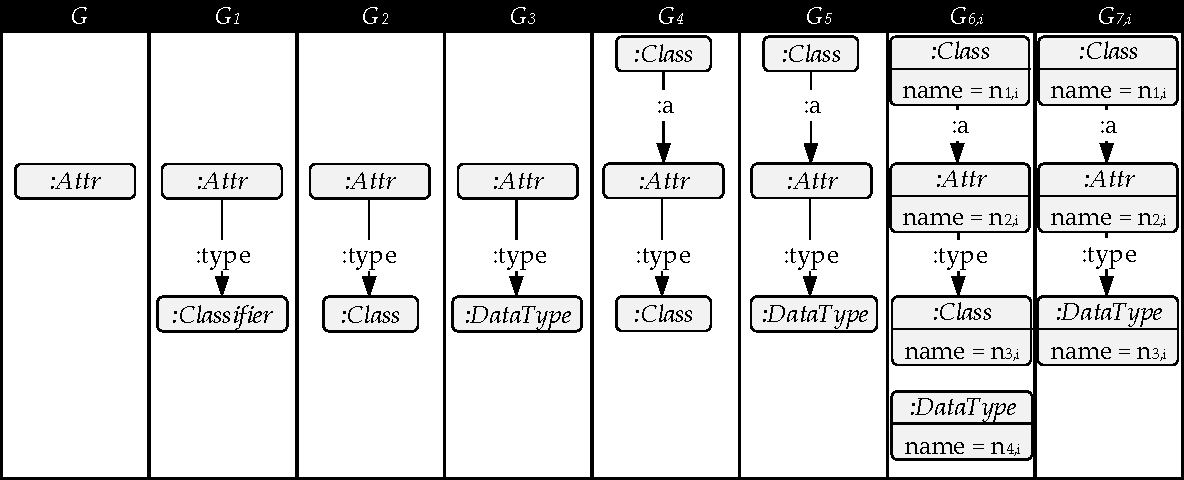
\includegraphics[width=\textwidth]{img/dc/extensions.pdf}
$Extensions(G,C)=\{\{G\},\{G_2,G_3\},\{G_4,G_3\},\{G_4,G_5\},\{G_{6,1},\ldots,G_{6,8},G_{7,1},\ldots,G_{7,5}\},\ldots\}$
\caption{$C$-extensions of Effective Atom \code{:Attr}}
\label{fig:c-extensions}
\end{figure}
\end{example}

\cref{fact:c-inc_c-ext} states that any extension of a $C$-inconsistent graph $G$ again leads to $C$-inconsistent graphs only yielding an empty extension and therefore, $C$-inconsistent graphs can be neglected in extensions.

%\nn{rename proposition to properties of C-Extensions that are demanden for the construction such that C-incosistent graphs do not need to be considered for extensions - additionally with $A=Extensions(G,C)$ with G C-inconsistent leads to $A \cup \varnothing$ AND all graphs in Extensions are not C-inconsistent except initial extension of c-inconsistent graphs - Remark 17 ins example einfuegen}

\begin{proposition}[C-Inconsistency in C-Extensions]
\label{fact:c-inc_c-ext}
Let $G$ be a graph, $C$ be a set of constraints, $E \in Extensions(G,C)$ be an extension of $G$ and $G_E \in E$ be an extended graph.
If $G_E$ is $C$-inconsistent, then $extend(G_E,\ac_P,m)=\varnothing$ for each constraint $\ac_P \equiv \vee_{i \in I} \exists (a_i\colon P \to C_i, \ac_{C_i})$ and match $m\colon P \to G_E \in \M$.
\envEndMarker
\end{proposition}

\begin{proof}
Let $G_E$ be a $C$-inconsistent graph, i.e., by \cref{def:inconsistent-graph} there exists a violation stable constraint $c \in C$ with $G_E \not\models c$.
$\M$-morphisms are closed under pushouts, i.e., $e\colon G_E \to G_E' \in \M$ in \cref{def:C-extension}, since, $f' \in \M$ and (1) is a pushout.
By \cref{def:violation-stab}, it follows that also $G_E' \not\models c$, i.e., also $G_E'$ is $C$-inconsistent.
By \cref{def:C-extension} it follows that $extend(G_E,\ac_P,m)=\varnothing$ for each constraint $\ac_P \equiv \vee_{i \in I} \exists (a_i\colon P \to C_i, \ac_{C_i})$ and match $m\colon P \to G_E \in \M$.
\end{proof}

\begin{remark}
By \cref{def:C-extension}, all graphs in $Extensions(G,C)$ are not $C$-inconsistent, except graph $G$ itself may be $C$-inconsistent as element of its initial extension $\{G\}$.
By following \cref{fact:c-inc_c-ext}, extending the initial extension for $C$-inconsistent graph $G$ via $extend(G,\_,\_)$ yields an empty extension $\varnothing \in Extensions(G,C)$.
Furthermore, contradictions in $C$ may also lead empty extensions $\varnothing \in Extensions(G,C)$, e.g., $G$ is extended via a constraint of $C$ leading to $C$-inconsistent graphs only that do not satisfy violation stable constraints of $C$.
In both cases, the existing empty extension $\varnothing$ of $G$ indicates that $G$ is not significant w.r.t. $\Lang(C)$.
\envEndMarker
\end{remark}

% \begin{remark}
% \label{rem:ext-fulfill}
% Note that for a given set of constraints $C$, only graphs are contained in
% extensions that are not $C$-inconsistent.
% This may lead to extension steps $E \Trans{extend(G_E \in E,c,\_)} E$ with
% constraint $c \in C$ that yield the same extension $E$, e.g., extension step
% $\{G_1\} \Trans{extend(G_1,c_5,\_)} \{G_1\}$ of extension $\{G_1\}$ in
% \cref{fig:c-extensions} with constraint $c_5$ in \cref{fig:constraints2}.
% Moreover, the extension step $E \Trans{extend(G_E,c,m)} E'$ that tries to
% extend a graph $G_E \in E$ via constraint $c \in C$ and match $m$ leads to an extension
% $E'= E \setminus \{G_E\}$ without $G_E$ if
% $G_E$ can not be extended at $m$ or all extensions are $C$-inconsistent. This may lead to the empty extension
% $\varnothing \in Extensions(G,C)$ for graphs $G$ that can not be embedded into
% graphs $G'$ ($G \xhookrightarrow{} G'$) such that $G' \models C$.
% \envEndMarker
% \end{remark}

% \begin{remark}
% If a constraint $\exists(P \trans{id} P, \vee_{i \in I} \exists (ac_i\colon P
% \to C_i, \true) )$ can be matched via morphism $m$ to a graph but morphisms
% $(m,ac_i)$ for some $i \in I$ are not compatible with the type inheritance, then
% the pushout (1) does not exist and we neglect the extension for the
% corresponding conclusion. If for all conclusions $ac_i$, morphisms $(m,ac_i)$
% are not compatible, then also the matched graph is neglected. Two morphisms $(m,ac_i)$
% are compatible with the type inheritance, if for all elements $e \in dom(m)=dom(ac_i)$ it holds that $m(e)$ is of the same type or a sub-type of $ac_i(e)$ or vice versa.
% \envEndMarker
% \end{remark}

For $C$-extension completeness it is sufficient to consider only the smallest graphs that occur in graphs $G \in \Lang(C)$, namely effective atoms, and from which more complex graphs can be constructed.
Atoms are the smallest graphs in the sense that they cannot be splitted into smaller sub-graphs.
With $Atoms(\ATG)$ we denote the set of atoms that are typed over an attributed type graph $\ATG$.
For (typed) attributed graphs the structure of each atom is given by either
\begin{enumerate*}[label=\itshape\alph*\upshape)]
\item an empty graph, or 
\item a single node, or 
\item a single edge together with source and target nodes, or
\item a single node attribute together with the corresponding node, or
\item a single edge attribute together with the corresponding edge and its source and target nodes.
\end{enumerate*} 
The idea of an atom $a$ is similar to the idea of an incremental monomorphism $f\colon I\rightarrowtail a$ that must exist with $I$ being the initial object (cf. \cite{DBLP:conf/wadt/CorradiniHHGN12}).
% Attributed graph morphisms $f\colon AG_1 \to AG_2$ of class
% $\mathcal{M}$ with $f=(f_G,f_D)$ are injective morphisms $f_G$ on the graph structure part and
% isomorphisms $f_D$ of algebras on the data part.
Note that all atoms in $Atoms(\ATG)$ share the same $\DSIG$-term algebra $T_\DSIG(X)$ such that the verification of domain completeness via \cref{thm:C-extensionCompleteness} is performed on the topmost level of $T_\DSIG(X)$ and therefore, can be instantiated to any concrete $\DSIG$-algebra for attributed graphs in $\Lang(C)$ and $\Lang(\GG)$ (Note that according to the general assumption, for domain completeness we assume that graphs in $\Lang(C)$ and $\Lang(\GG)$ share the same concrete $\DSIG$-algebra up to isomorphism).

\vspace{2ex}
\parpic[r][r]{
$
\SelectTips{cm}{}
     \xymatrix@R-4ex@C-4ex{
     & B \ar[dr]^{b'} & \\
     I \ar[ur]^{b} \ar[dr]_{c} & (1) & a \\
     & C \ar[ur]_{c'} & 
     }
$
}
\vspace{-2ex}
\begin{definition}[Atom]
\label{def:atom}
A \emph{graph $a$ is an atom}\index{atom}, if for each pushout (1) on the right with morphisms $b,c \in \M$ it is true that $b' \colon B \to a$ is an isomorphism or $c' \colon C \to a$ is an isomorphism.
Let $\ATG=(\TG,Z)$ be an attributed type graph with type graph $\TG$ and the final $\DSIG$-algebra $Z$ of data signature $\DSIG=(S,\OP)$ with sorts $S$ and operations $\OP$.
With $Atoms(\ATG)=\{(a=(G,T_{\DSIG}(X)),\type_G\colon a \to \ATG) \mid a \n{ is an atom},(\n{for all }e \in E^G_j\colon t^G_j(e) \in X)_{j \in \{NA,EA\}}, X=(X_s)_{s \in S} \n{ being a family of infinite sets } X_s \n{ of variables for each sort }s \in S\}$ we define the set of atoms by attributed graphs that are typed over $\ATG$ and that share the same $\DSIG$-term algebra $T_{\DSIG}(X)$ with an infinite set of variables $X_s$ for each sort $s \in S$ where each node attribute $E^G_{NA}$ and each edge attribute $E^G_{EA}$ has a variable as attribute value.
\envEndMarker
\end{definition}

Given a set of constraints $C$ that are typed over attributed type graph $\ATG$, then with $EAtoms(C)$ we denote the set of effective atoms w.r.t. language $\Lang(C)$.
Effective atoms are those atoms in $Atoms(\ATG)$ that occur in graphs $G \in \Lang(C)$.

\begin{definition}[Effective Atom]
\label{def:eatom}
Given language $\Lang(C)$ over attributed type graph $\ATG$ and constraints $C$, an \emph{atom $a \in Atoms(ATG)$ is effective w.r.t. $\Lang(C)$}\index{atom!effective}, if there exists an inclusion $i\colon a \to G \in \M$ for some graph $G \in \Lang(C)$.
With $EAtoms(C)=\{a \mid a \in Atoms(\ATG), a \n{ is effective w.r.t. }\Lang(C)\}$ we denote the set of effective atoms w.r.t. $\Lang(C)$.
\envEndMarker
\end{definition}

\begin{example}[Effective Atom]
Given the constraints $C$ for UML class diagrams in \cref{sec-gt-gc,ex:sec-gc-gc:gc_UML_CD}, then the effective atoms w.r.t. $\Lang(C)$ are those atoms in $Atoms(\TG_{\CD})$ that fulfill the domain constraints for abstract types from \cref{ex:sec-gc-gc:gc_UML_CD}.
Graphs $G,G_2$ and $G_3$ in \cref{fig:c-extensions} are effective atoms w.r.t. $\Lang(C)$.
Graph $G_1$ is an atom but not effective, since, \code{Classifier} is an abstract type and therefore, $G_1$ violates the constraints for abstract types.
Graphs $G_4$ to $G_{7,5}$ are not atoms.
\envEndMarker
\end{example}

For $C$-extension completeness, in practice we consider atoms up to isomorphism only.
Given a set of constraints $C$ that are typed over type graph $\ATG$, then $C$-extension completeness of a given language $\Lang$ over $\ATG$ states that for all effective atoms w.r.t. $\Lang(C)$ that are typed over $\ATG$, an extension via constraints $C$ can be found that is in $\Lang$.

\begin{definition}[$C$-Extension Completeness]
\label{def:C-extensionCompleteness}
Let $C$ be a set of constraints typed over $\ATG$ and $C' \subseteq C$ be the contained constraints that are designated for general satisfaction.
Then, a language $\Lang$ over $\ATG$ is called \emph{$C$-extension complete}\index{$C$-extension completeness}, if $\forall a \in EAtoms(C). \exists S \in Extensions(a, C')$ such that $S \subseteq \Lang$.
\envEndMarker
\end{definition}

\begin{example}[$C$-Extension Completeness]
\label{ex:c-extension-compl}
\begin{figure}[tb]
\centering
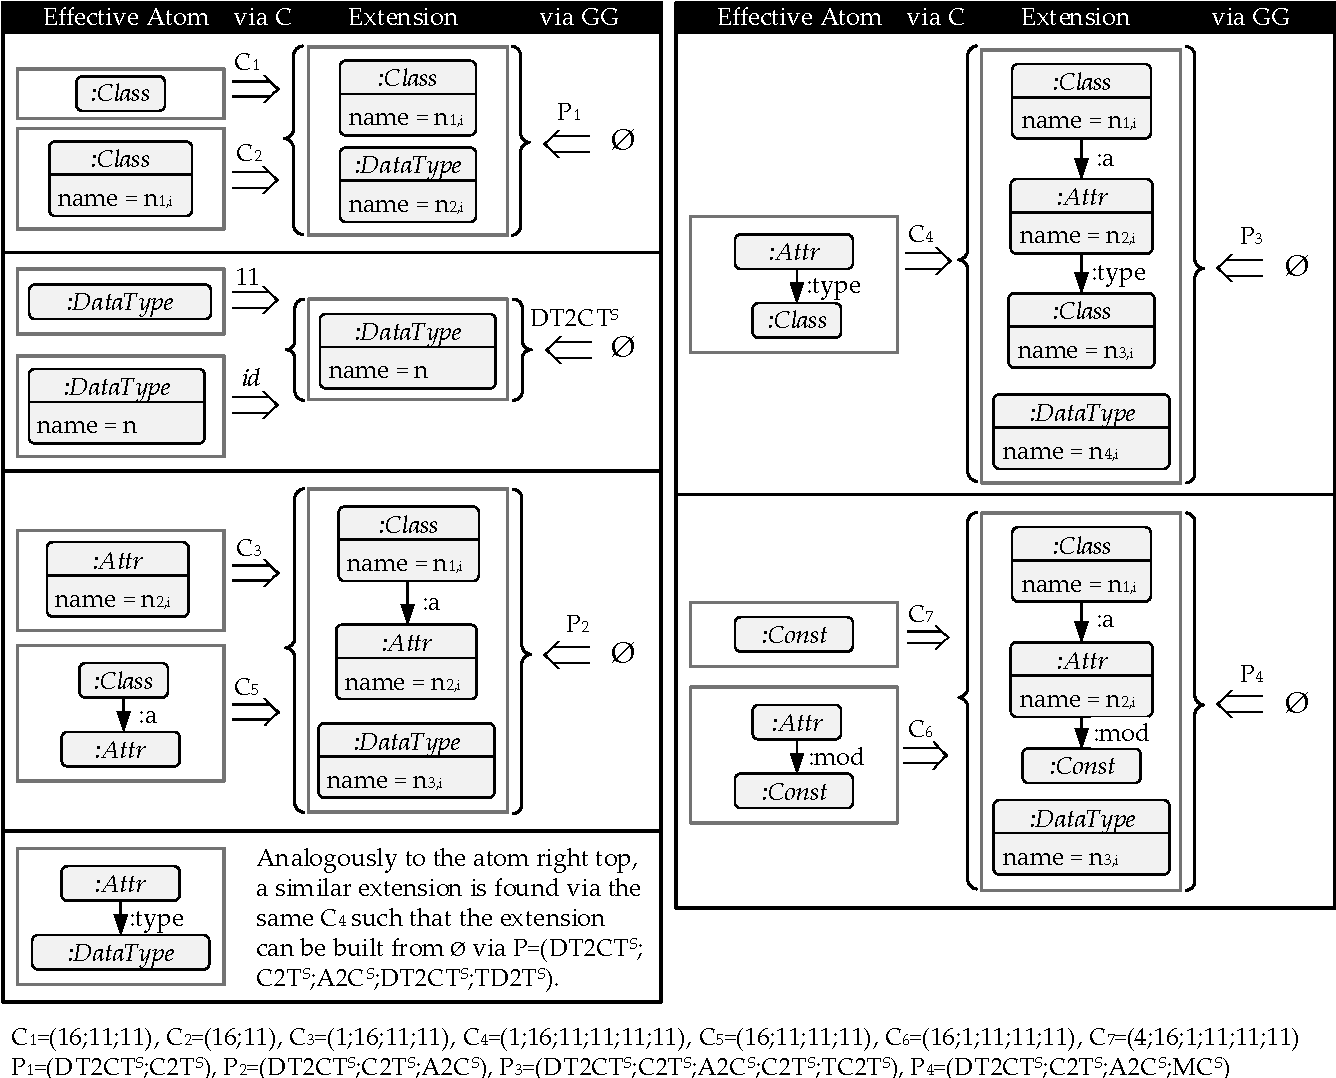
\includegraphics[width=\textwidth]{img/dc/example_compl}
\caption{Verifying $C$-Extension Completeness of Language $\Lang(\GG)$ for UML Class Diagrams}
\label{fig:eatoms_check}
\end{figure}
Given the rules $P$ for creating UML class diagrams from \cref{sec-gt-trafo,ex:sec-gt-trafo:trafo} together with grammar $\GG=(\varnothing,P)$ that is typed over $\TG_\CD$ in \cref{sec-gt-graphs,fig:sec-gt-graphs:atg} and the constraints $C$ for class diagrams typed over $\TG_\CD$ from \cref{sec-gt-gc,ex:sec-gc-gc:gc_UML_CD}.
We show $C$-extension completeness of language $\Lang(\GG)$ over $\TG_\CD$. 
For each effective atom in $EAtoms(C)$ an extension via constraints $C$ must be constructed that is a subset of language $\Lang(\GG)$.
Similarly to \cref{ex:c-extensions}, we write the actual constraints but mean their instances according to \cref{def:C-extension} and furthermore, each graph with attribute values $n_{1,i}$ to $n_{4,i}$ in \cref{fig:eatoms_check} represents a set of graphs that contains all combinations of equal and unequal values $n_{1,i}$ to $n_{4,i}$ except equal values for $n_{1,i}$ and $n_{3,i}$ if both represent the \code{name}s of distinct \code{Class}es.
An extension is a subset of $\Lang(\GG)$, if all graphs of the extension can be constructed via rules $P$ from start graph $\varnothing$ of $\GG$.
The effective atoms $EAtoms(C)$ are given by graph $G$ in \cref{fig:c-extensions} together with the effective atoms in \cref{fig:eatoms_check}.
For atom $G$, extension $\{G_{6,1},\ldots,G_{6,8},G_{7,1},\ldots,G_{7,5}\} \in Extensions(G,C)$ can be constructed by extending $G$ via constraints $(8;1;1;11;11;11;16;11;11;11;11)$ of $C$ successively (cf. \cref{ex:c-extensions}).
Each graph of the extension can be constructed by applying rules \code{(DT2CT^S;C2T^S;A2C^S;C2T^S;TC2T^S)} or \code{(DT2CT^S;C2T^S;A2C^S;TD2T^S)} successively with starting at the empty start graph $\varnothing$ of $\GG$.
All other effective atoms are also successfully checked as depicted in \cref{fig:eatoms_check}.
Therefore, language $\Lang(\GG)$ is $C$-extension complete.
% \begin{itemize}
%   \item Atom \xymatrix{*+[F]\txt{:Class}} can be extended with constraints $c_8$
%   to extension $\left\{\xymatrix{*+[F]\txt{:Class(name=n)}}\right\}$ which can be
%   constructed by source rule \code{1:~C2T$_S$}.
%   \item Atom \xymatrix{*+[F]\txt{:Class(name=n)}} can be directly constructed by
%   source rule \code{1:~C2T$_S$}.
%   \item Atom \xymatrix{*+[F]\txt{:PrimitiveType}} can be extended with
%   constraint $c_8$ to extension
%   $\left\{\xymatrix{*+[F]\txt{:PrimitiveType(name=n)}}\right\}$ which can be constructed by
%   source rule \code{2:~PT2CT$_S$}
%   \item Atom \xymatrix{*+[F]\txt{:PrimitiveType(name=n)}} can be
%   directly constructed by source rule \code{2:~PT2CT$_S$}
%   \item Atom \xymatrix{*+[F]\txt{:Attribute(name=n)}} is checked analogously to \cref{ex:c-extension-compl} but this time the extensions for the \code{name} attribute are omitted.
%   \item Atom \xymatrix{*+[F]\txt{:Attribute(is\_primary=true)}} can be extended with constraints in the given order $(c_{10},c_1,c_8^*)$ leading to extension \begin{align*}
%   \left\{\xymatrix{*+[F]\txt{:Class\\(name=n1)} \ar[r]^-{:attrs} & *+[F]\txt{:Attribute\\(is\_primary=true,\\name=n2)} \ar[r]^-{:type} & *+[F]\txt{:PrimitiveType\\(name=n3)}} \right\}
%   \end{align*} which can be constructed by applying the following source rules in the given order: (\code{1:~C2T$_S$}, \code{2:~PT2CT$_S$}, \code{3:~PA2C$_S$}, \code{4:~AM2CM$_S$}, \code{5:~P2PK$_S$}).
%   \item Atom \xymatrix{*+[F]\txt{:Attribute(is\_primary=false)}} can be extended with constraints in the given order $(c_5,c_4,c_8^*)$ leading to an extension with two graphs \begin{align}
%   G_1=\xymatrix{*+[F]\txt{:Attribute\\(is\_primary=false,\\name=n1)} \ar[r]^-{:type} & *+[F]\txt{:PrimitiveType\\(name=n2)}}\\
%   G_2=\xymatrix{*+[F]\txt{:Attribute\\(is\_primary=false,\\name=n1)} \ar[r]^-{:type} & *+[F]\txt{:Class\\(name=n2)}}
%   \end{align} which can be constructed by applying the following source rules in the given order: (\code{2:~PT2CT$_S$}, \code{3:~PA2C$_S$}, \code{7:~NP2E$_S$}) for $G_1$ and (\code{1:~C2T$_S$}, \code{6:~NPA2C$_S$}, \code{7:~NP2E$_S$}) for $G_2$.
%   \item Analogously, atoms \xymatrix{*+[F]\txt{:Class} \ar[r]^-{:attrs}& *+[F]\txt{:Attribute}}, \xymatrix{*+[F]\txt{:Attribute} \ar[r]^-{:type}& *+[F]\txt{:Class}} and \xymatrix{*+[F]\txt{:Attribute} \ar[r]^-{:type}& *+[F]\txt{:PrimitiveType}} can be checked.
% \end{itemize}
\envEndMarker
\end{example}

% \begin{remark}
% In the
% presented setting, only language inclusions $\Lang_1=\Lang(\ATG,C) \subseteq
% \Lang_2=\Lang(\ATG,\GG,C)$ between languages with the same set of constraints
% $C$ are considered. Therefore, we are only interested in the C-extension completeness
% of languages $\Lang_2$ where $\Lang_2$ is restricted
% by $C$. Consequently, for efficiency reasons the derivation and checking of
% extensions can be stopped at extensions that violate negative constraints in $C$, since,
% these extensions and all other derivations of such extensions are not in
% $\Lang_2$.
% \envEndMarker
% \end{remark}

%A union $A +_I B$ of two objects $A$ and $B$ is 
%constructed by finding an intersection $I$ with embeddings (\M-morphisms)
%$a \colon I \to A, b\colon I\to B$ and constructing the pushout of $a$ and $b$ 
%yielding the pushout object $C = A +_I B$.

%\begin{definition}[Closure under Union]
%\label{def:closedness-union}
%A language $\Lang$ is closed under union, if any union $A +_I B$ of two elements $A,B \in \Lang$
%is contained in $\Lang$.
%\envEndMarker
%\end{definition}

%\begin{lemma}[C-Extension Completeness and closure]
%\label{lem:C-extension-closure}
%Let $C$ be a set of constraints typed over $TG$ and 
%$\Lang$ be a $C$-extension complete language that is closed under union.
%Then, $\Lang(TG,C) \subseteq \Lang$.
%\envEndMarker
%\end{lemma}
%
%\begin{proof}
%to be done - Benjamin/Nico??
%\end{proof}

% \longversionMarker{
% \begin{remark}
% Note that the problem of whether a language is C-extension completeness is only
% semi-decidable but not decidable in general. If a language
% $\Lang$ is C-extension complete, then for each effective atom
% an extension can be found that is in $\Lang$ but for languages that are not
% C-extension complete we may not neglect this fact. Note that for the generation
% of extensions, for each constraint and match only one instance of the constraint
% must be considered which is obtained by the $\E$--$\M$-factorization of the
% match morphism (cf.\cref{cor:AC-schemata-satisfaction}).
% In practice, the size of the graphs in $\Lang$ is limited to a maximal number \emph{MAX} of graph elements in order to obtain decidability of the problem. This reduces the verification to extensions up to a size of \emph{MAX} graph elements.
% \envEndMarker
% \end{remark}
% }

In addition to $C$-extension completeness another property called $C$-conflict-freeness of marking rules is neccessary in order to verify full language inclusions $\Lang(C) \subseteq \Lang(\GG)$ of domain completeness.
Based on the notions of translation attributes in \cref{sec-mt-tgg,rem:sec-mt-tgg:tr_attr} and consistency creating (CC) rules in \cref{sec-msynch-tgg,def:sec-msynch-tgg:cc_rule}, we define marking rules for non-deleting flat grammars with application conditions in \cref{def:marking-rule}.
In the context of marking rules, we take marking attribute as synonym for translation attribute.
For a non-deleting grammar $\GG$, the set of marking rules $m(\GG)$ contains for each rule $r \in \GG$, a marking rule $m(r)$.
Analogously to CC rules, marking rules are derived from rules by adding marking attributes with value $\False$ (false) or $\True$ (true) to all elements (nodes, edges or attributes) of the rule.
Whenever rule $r$ creates an element, then marking rule $m(r)$ preserves this element and updates its marking attribute from $\False$ to $\True$, denoted by $[\False => \True]$.
Whenever rule $r$ preserves an element, then marking rule $m(r)$ also preserves this element and leaves its marking attribute set to $\True$.
Thus, marking rules are deleting on the marking attributes and allow a conflict analysis of (common) created elements which cannot be performed directly on the non-deleting rules themselves.
Furthermore, all elements of the application condition of rule $r$ that are not contained in the left-hand side of the rule need to be extended by a marking attribute with value $\True$.
Therefore, we use the concept of $\True$-extended application conditions from \cref{sec-mt-tgg,def:sec-mt-tgg:T-Ext} and restrict it from triple graphs to flat graphs by omitting the triple components $X$.

% \begin{remark}[Well-Definedness of $\True$-Extension]
% Note that $P' +_P C$ denotes the gluing of graphs $P'$ and $C$ over shared graph $P$ (constructed as a pushout).
% The $\True$-Extension construction is well-defined in the category $\AGraphs_{\ATGI}$, as, morphism $P \to P'$ is an identity on the data part by construction of graphs with marking attributes (i.e., $a_D$ can be used for $a_E$) and $\AGraphs_{\ATGI}$ is $\M$-adhesive (i.e., pushouts exist along $\M$-morphisms and $\M$-morphisms are closed under pushouts, thus, $\inc'_P$ is an inclusion). 
% \envEndMarker
% \end{remark}

\begin{definition}[Marking Rule]
\label{def:marking-rule}
Given a non-deleting rule $p=\nobreak(\ol{p}\colon L \xhookrightarrow{} R,\ac_L)$, the \emph{marking rule $m(p)=(L_M \xhookleftarrow{l_M} K_M \xhookrightarrow{r_M} R_M,\ac_{L_M})$ of $p$}\index{marking rule} is constructed component-wise for $L_M,K_M,R_M$ and $\ac_{L_M}$ with induced inclusions $l_M,r_M$ and $L_M := R \oplus \Att_{\ol{p}(L)}^{\True} \oplus \Att_{R\setminus \ol{p}(L)}^{\False}, K_M := R \oplus \Att_{\ol{p}(L)}^{\True}, R_M := R \oplus \Att_R^{\True}$ and $\ac_{L_M}=\tExt(\ac_L,L_M)$.
Let $\GG=(S,P)$ be a non-deleting graph grammar.
With $m(\GG)=\{m(p) \mid p \in P\}$ we define the set of marking rules for all rules in $\GG$.
\envEndMarker
\end{definition}

\begin{remark}[Termination of Transformation System $m(\GG)$]
\label{rem:sec-dc-verification:term_marking_rules}
Although marking rules are not directly applied for verifying domain completeness, we state the following interesting property:
If all rules $p=(L \xhookrightarrow{} R,\ac_L)$ of a non-deleting grammar $\GG$ are non-trivial in the sense that $L$ and $R$ are not isomorphic ($L \not\cong R$) and therefore, each rule creates at least one element, then the transformation system $m(\GG)$ of marking rules is terminating for finite graphs, since, each application of marking rules updates the marking attributes of at least one graph element from $\False$ to $\True$ as long as all graph elements are marked with $\True$ or no marking rule is applicable anymore.
\envEndMarker
\end{remark}

\begin{example}[Marking Rule]
\label{ex:sec-dc-verification:marking_rule}
\begin{figure}[tb]
\centering
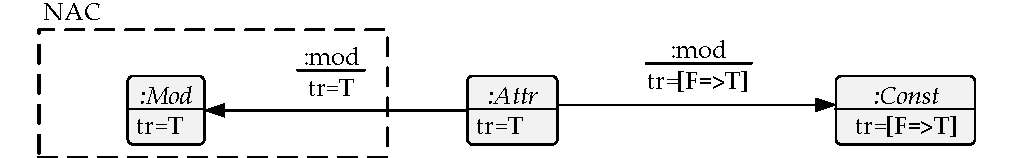
\includegraphics[width=.9\textwidth]{img/dc/markingrule-VOLT.pdf}
\caption{Marking Rule $m(\code{4}^S)$ of Rule $\code{4}^S$ for UML Class Diagrams}
\label{fig:sec-dc-verification:marking_rule}
\end{figure}
The marking rule $m(\code{4}^S)$ of source rule $\code{4}^S$ from \cref{sec-gt-trafo,ex:sec-gt-trafo:trafo} is given by the rule in \cref{fig:sec-dc-verification:marking_rule}.
Marking attributes $\tr$ are added to all elements and they are updated from $\False$ to $\True$ ($[\False => \True]$) for those elements that are created by rule $\code{4}^S$ while the marking attributes of all other elements are initially set to $\True$ and remain unchanged.
\envEndMarker
\end{example}

The $C$-conflict-freeness of marking rules is checked based on critical pair analysis.
According to \cref{def:consistent-critical-pair} and similarly to $C$-inconsistent graphs, a critical pair $(K_1 \TransB{} O \Trans{} K_2)$ is $C$-inconsistent if graph $O$ does not satisfy a constraint in $C$ that is violation stable under embedding.
$C$-inconsistent critical pairs do not need to be analysed for verifying domain completeness, since, such critical pairs and any of their embeddings into larger contexts do not occur in graphs $G \in \Lang(C)$.
The marking rules are $C$-conflict-free, if for each critical pair $(K_1 \TransB{(p_1,o_1)}\nobreak O \Trans{(p_2,o_2)} K_2)$ that is not $C$-inconsistent with marking rules $p_1$ and $p_2$, the rules and matches are the same $(p_1=p_2,o_1=o_2)$ (cf. \cref{def:cf-marking-rules}).

\begin{definition}[$C$-Inconsistent Critical Pair]
\label{def:consistent-critical-pair}
Let $C$ be a set of constraints. 
A \emph{critical pair $(K_1 \TransB{} O \Trans{} K_2)$ is $C$-inconsistent}\index{critical pair!$C$-inconsistent}, if conflict graph $O$ is $C$-inconsistent. 
\envEndMarker
\end{definition}

\parpic[r][r]{
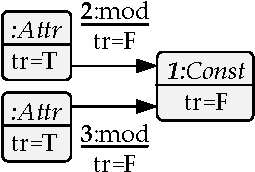
\includegraphics[width=.23\textwidth]{img/dc/c_inc_cp.pdf}
}
\vspace*{-.25cm}
\begin{example}[$C$-Inconsistent Critical Pair]
\label{ex:c_inc_cp}
The figure on the right presents the conflict graph $O$ of the critical pair $(K_1 \TransB{(m(4^S),m_1)} O \Trans{(m(4^S),m_2)} K_2)$ with marking rule $m(4^S)$ from \cref{ex:sec-dc-verification:marking_rule}.
Transformation $O \Trans{(m(4^S),m_1)} K_1$ updates the marking attributes of node \code{1:Const} and edge \code{2:mod} and $O \Trans{(m(4^S),m_2)} K_2$ updates the marking attributes of \code{1:Const} and edge \code{3:mod} from $\False$ to $\True$.
This corresponds to a delete-use conflict at node \code{1:Const} in $O$, since, both transformations change its marking attribute where the attribute is deleted at first and added with the new value $\True$ afterwards.
However, by assuming the constraints $C$ for UML class diagrams from \cref{sec-gt-gc,ex:sec-gc-gc:gc_UML_CD}, the critical pair is $C$-inconsistent, since, $O \not\models 7$ and constraint $7 \in C$ is violation stable under embedding, i.e., graph $O$ is $C$-inconsistent (cf. \cref{ex:constraints-violation-stable}).
\envEndMarker
\end{example}

Analogously, to significant graphs, we introduce significant critical pairs.
A critical pair is significant, if it occurs in graphs $G \in \Lang(C)$.
Also analogously to significant and $C$-inconsistent graphs, $C$-inconsistent critical pairs are only a subset of not significant critical pairs but can be identified more efficiently.

% Significant critical marking pairs describe pairs $P_1 \TransB{(m(p_1),m_1)} K \Trans{(m(p_2),m_2)} P_2$ of transformations via marking rules $m(p_1),m(p_2)$ where the sub-graph $K'$ of $K$ marked with $\True$ can be created via $P$ (possibly in bigger contexts $K''$) and $K'$ ($K''$) is contained in graphs of $\Lang(\TG,C)$ (and creating rules $p_1,p_2 \in P$ are applicable to $K''$ with matches compatible to inclusion $K' \xhookrightarrow{} K''$).
% Thus, we only consider parallel dependent transformation steps that may occur when creating graphs of $\Lang(\TG,C)$ via $P$.
\begin{definition}[Significant Critical Pair]
\label{def:sig_crit_pair}
Let $C$ be a set of constraints, $\GG$ be a non-deleting grammar and $m(\GG)$ be the corresponding set of marking rules.
A \emph{critical pair $(K_1 \TransB{(p_1,m_1)} O \Trans{(p_2,m_2)} K_2)$ for marking rules $p_1,p_2 \in m(\GG)$ is significant w.r.t. $\Lang(C)$}\index{critical pair!significant}, if conflict graph $O$ is significant w.r.t. $\Lang(C)$.
\envEndMarker
\end{definition}

\begin{remark}[Relationship between $C$-Inconsistent \& Significant Critical Pairs]
\label{rem:sec-dc-verification:rel_critical_pair}
Similarly to the relationship between $C$-inconsistent and significant graphs in \cref{rem:sec-gc-verification}, by definition, each $C$-inconsistent critical pair is not significant w.r.t. $\Lang(C)$.
Furthermore, each critical pair that is significant w.r.t. $\Lang(C)$ is not $C$-inconsistent.
The other directions do not hold in general.
\envEndMarker
\end{remark}

\begin{figure}[tb]
\centering
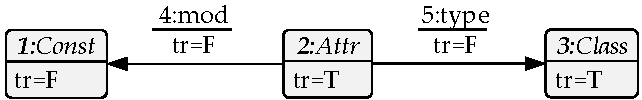
\includegraphics[width=.65\textwidth]{img/dc/sign_cp.pdf}
\caption{Significant Critical Pair}
\label{fig:sec-dc-verification:sign_critical_pair}
\end{figure}

\begin{example}[Significant Critical Pair]
\label{ex:sign_cp}
The graph in \cref{fig:sec-dc-verification:sign_critical_pair} presents the conflict graph $O$ of the critical pair $(K_1 \TransB{(m(4^S),m_1)} O \Trans{(m(6^S),m_2)} K_2)$ with marking rules $m(4^S)$ and $m(6^S)$ of the rules in \cref{sec-gt-trafo,ex:sec-gt-trafo:trafo}.
Transformation $O \Trans{(m(4^S),m_1)} K_1$ updates the marking attributes of edge \code{4:mod} and node \code{1:Const} from $\False$ to $\True$ leading to a graph pattern which is forbidden by the NAC of rule $m(6^S)$ with match $m_2$ (change-forbid attribute conflict).
Given the constraints $C$ for UML class diagrams from \cref{sec-gt-gc,ex:sec-gc-gc:gc_UML_CD}, then the critical pair is not $C$-inconsistent, since, $O$ does not violate a constraint $c \in C$ which is violation stable under embedding.
However, the critical pair is not significant, since, graph $O$ is not significant w.r.t. $\Lang(C)$ (cf. \cref{ex:sec-dc-verification:inc_sig_graph}).
\envEndMarker
\end{example}

% \begin{lemma}[C-Extension Completeness for Conflict-free Grammar]
% \label{lem:conflictFree}
% Let $C$ be a set of constraints $C$ and
%  $\GG$ be a graph grammar. 
% If all marking rules $p \in m(GG)$ are $C$-conflict-free
% and $\Lang(GG)$ is $C$-extension complete, then 
% $\Lang(TG,C) \subseteq \Lang(GG)$.
% \envEndMarker
% \end{lemma}

%\begin{corollary}[Closure for Conflict-free Grammar]
%\label{cor:conflictFree-closure}
%Let $\GG$ be a non-deleting graph grammar
%and $C$ be a set of constraints, such that 
%$\Lang(\GG,C) = \Lang(\GG)$.
%If for each critical pair of
%$m(\GG)$ that is not C-inconsistent the rules and matches are the same and $m(\GG)$ is
%terminating, then $\Lang(GG,C)$ is closed under union.
%\envEndMarker
%\end{corollary}
%
%\begin{proof}
%to be done using \cref{lem:conflictFree-closure}.
%\end{proof}





% \begin{definition}[Graph with marking attributes]
% An attributed graph $\AG=(G,D)$ is a graph with marking attributes, if $G$ is
% extended by one boolean marking attribute for each element in $G$ (node or edge)
% and by one boolean marking attribute for each attribute of an element with
% $ATT_G$ being the extension of $G$. $ATT_G^v$ with $v=\True$ or $v=\False$ denotes a
% graph where all marking attributes are set to true or false. With $AG \oplus
% ATT_{G_0}^v$ and $G_0 \subseteq G$ we denote an attributed graph AG where all
% attributes of the subgraph $G_0$ are set to true or false.
% \end{definition}

\begin{figure}[tb]
\centering
% \includegraphics[width=.55\textwidth]{figs/agg.png}
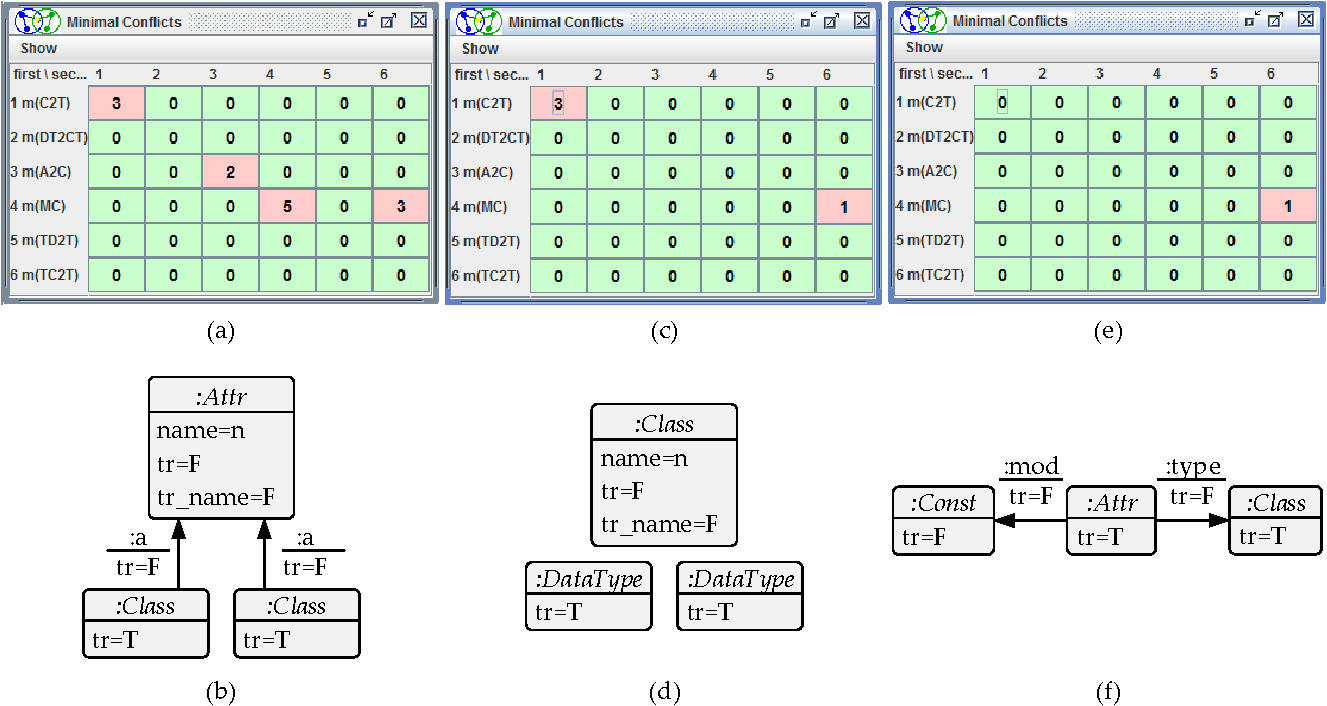
\includegraphics[width=\textwidth]{img/dc/agg.pdf}
\caption{Result of Conflict Analysis for Marking Rules of UML Class Diagrams in AGG}
\label{fig:agg}
\end{figure}

\begin{definition}[$C$-Conflict-Freeness of Marking Rules]
\label{def:cf-marking-rules}
Let $C$ be a set of constraints and let $m(\GG)$ be the marking rules of a non-deleting grammar $\GG$.
Then, \emph{$m(\GG)$ is $C$-conflict-free}\index{marking rule!$C$-conflict-freeness}, if for each critical pair $(K_1 \TransB{(p_1,o_1)}\nobreak O \Trans{(p_2,o_2)} K_2)$ that is significant w.r.t. $\Lang(C)$ (or not $C$-inconsistent) with $p_1,p_2 \in m(\GG)$ it is true that the rules and matches are the same ($p_1=p_2,o_1=o_2$) (or it is true that the critical pair is strictly confluent).
\envEndMarker
\end{definition}

\begin{remark}[$C$-Conflict-Freeness of Marking Rules]
\label{rem:sec-dc-verification:conf_free_mr}
The critical pairs in \cref{def:cf-marking-rules} need to be significant or not $C$-inconsistent.
Analogously to \cref{rem:sec_dc-verification:c-ext}, claiming that the critical pairs are significant is more accurate for verifying domain completeness based on $C$-conflict-freeness of marking rules in \cref{def:cf-marking-rules,thm:C-extensionCompleteness}, since, critical pairs may be not $C$-inconsistent and not significant at the same time (cf. \cref{ex:sign_cp}).
While not $C$-inconsistent critical pairs are considered in $C$-conflict-freeness of marking rules, not significant critical pairs are not considered.
However, claiming that the critical pairs are not $C$-inconsistent can be checked more efficiently.
Furthermore, claiming that each critical pair is strictly confluent is a stronger condition and harder to check than claiming that each critical pair is of same rules and same matches.
Each critical pair of same rules and same matches is directly strict confluent by definition.
\envEndMarker
\end{remark}

\begin{example}[$C$-Conflict-Freeness of Marking Rules]
\label{ex:conflict-freeness-marking-rules}
The AGG-tool \cite{AGG} is used to help verifying $C$-conflict-freeness of marking rules $m(\GG)$ for grammar $\GG=(S,P)$ with rules $P$ for UML class diagrams from \cref{sec-gt-trafo,ex:sec-gt-trafo:trafo} and constraints $C$ for UML class diagrams from \cref{sec-gt-gc,ex:sec-gc-gc:gc_UML_CD}.
AGG enables to analise conflicts of rules, outputs all existing critical pairs and allows to ignore
\begin{enumerate*}
\item critical pairs of same rules and same matches,
\item critical pairs that violate multiplicity constraints, and
\item critical pairs that are directly strict confluent.
\end{enumerate*}
\cref{fig:agg} depicts the result of the analysis for the marking rules $m(\GG)$ of UML class diagrams.
\cref{fig:agg} (a) depicts all 13 critical pairs of marking rules $m(\GG)$ (red boxes) while ignoring all critical pairs of same rules and same matches.
\cref{fig:agg} (b) depicts the conflict graph of the critical pair of rule $\code{3}^S$ that updates the marking attributes of node \code{:Attr} and edges \code{:a} in parallel while matching differently to both \code{:Class} nodes.
The conflict graph violates multiplicity constraint \code{2} which is violation stable under embedding (cf. \cref{ex:constraints-violation-stable}).
Therefore the conflict graph is $C$-inconsistent implying further that the critical pair is $C$-inconsistent.
\cref{fig:agg} (c) depicts all four critical pairs of marking rules $m(\GG)$ while additionally ignoring all critical pairs that violate the multiplicity constraints in $C$.
\cref{fig:agg} (d) depicts the conflict graph of the critical pair of rule $\code{1}^S$ that updates the marking attributes of node \code{:Class} in parallel while matching differently to both \code{:DataType} nodes.
The conflict graph is not $C$-inconsistent, particularly it respects the multiplicity constraints.
However, the conflict graph is directly strict confluent, i.e., the critical pair is directly strict confluent.
\cref{fig:agg} (e) depicts the only critical pair of marking rules $m(\GG)$ while additionally ignoring all critical pairs that are directly strict confluent.
\cref{fig:agg} (f) depicts the conflict graph of the critical pair of rules $\code{4}^S$ and $\code{6}^S$ that updates the marking attributes of node \code{:Const} and edges \code{:mod}, \code{:type} in parallel while matching node \code{:Attr} in common.
The critical pair is not strictly confluent due to the NAC of rule $\code{6}^S$.
Furthermore, the critical pair is not $C$-inconsistent, particularly it does not violate the multiplicity constraints in $C$.
However, the critical pair is not significant (cf. \cref{ex:sign_cp}).
Therefore, the marking rules $m(\GG)$ of UML class diagrams are $C$-conflict-free.
\envEndMarker
\end{example}

% \begin{fact}[Characterisation of Grammars with C-conflict-free Marking Rules]
% Let $GG=(\ATG,\SG,P)$ be a grammer with non-deleting rules $P$ typed over
% $\ATG$ and let $C=C^{IN} \cup C^{OUT} \cup C^{Att}$ be a set of
% multiplicity constraints. The constraints in $C^{IN(OUT)}$ claim for a set of
% edge types $E(C^{IN(OUT)})$ that for all types $t \in E(C^{IN(OUT)})$, each node
% may have at most one incoming (outgoing) edge of type $t$. The
% constraints in $C^{Att}$ claim for a set of attributes $Att(C^{Att})$ that
% for all attributes $a \in Att(C^{Att})$, each node may have at most one
% attribute $a$.The marking rules $m(\GG)$ are C-conflict free iff for each rule
% $p \in P$:
% \begin{itemize}
%   \item $p$ creates at most one node of each type, and no other rule $p'
%   \in P$ creates nodes of the same types, or
%   \item 
% \end{itemize}
% \envEndMarker
% \end{fact} 

The main result for verifying domain completeness is stated by \cref{thm:C-extensionCompleteness}.
Intuitively, the language inclusion $\Lang(C) \subseteq \Lang(\GG)$ holds if each graph $G \in \Lang(C)$ can be decomposed into its atoms $a \subseteq G$ such that for each atom $a$ an extension $E$ can be constructed via constraints $C$ that is contained in $\Lang(\GG)$ and the composition of the extensions leads to graph $G$ in $\Lang(\GG)$ again by applying the rules of grammar $\GG$.
The verification approach requires that all productions of grammar $\GG$ are non-trivial.
For non-trivial productions we refer to \cref{rem:sec-dc-verification:term_marking_rules}.

\begin{theorem}[Domain Completeness]
\label{thm:C-extensionCompleteness}
\index{domain completeness!verification}
Let $\Lang(C)$ be a language over type graph $\ATG$ and constraints $C$ in $\M$-normal form and let $\Lang(\GG)$ be a language over $\ATG$ and non-deleting grammar $\GG=(\varnothing,P)$ with empty start graph $\varnothing$, all productions $p \in P$ being non-trivial and where all application conditions in productions $P$ are in $\M$-normal form.
If the marking rules $m(\GG')$ are $C$-conflict-free and $\Lang(\GG')$ is $C$-extension complete where $\GG'=(\varnothing',P)$ with $\varnothing'$ being the empty start graph with $\DSIG$-term algebra $T_\DSIG(X)$, then domain completeness holds for almost injective matches $m \in \morO$, i.e., it holds that $\Lang(C) \subseteq \Lang(\GG)$.
\envEndMarker
\end{theorem}

\begin{proof}[Idea]
Let $G \in \Lang(C)$.
Graph $G$ is abstracted to a graph $G_A$ with $\DSIG$-term algebra.
$G_A$ can be decomposed into its atoms $Atoms(G_A)$ by \cref{lemma:union-atoms}.
$C$-extension completeness of $\Lang(\GG')$ ensures that each atom can be extended via $C$ such that the extension can be created via grammar $\GG'$.
Furthermore, there is a gluing of all extensions leading to graph $G_A$ again by \cref{lem:union-ext-atoms}.
By the equivalence of marking and transformation sequences in \cref{lem:equivalence-marking-emptySG}, each extension can be fully marked with $\True$.
The $C$-conflict freeness of the marking rules $m(\GG')$ allows to apply confluence results and we derive a marking sequence that fully marks $G_A$. 
Thus by \cref{lem:equivalence-marking-emptySG}, there is a transformation sequence $\varnothing' \Trans{*} G_A$ via $P$.
By \cref{lem:atiti}, there is a transformation $\varnothing \Trans{*} G$ via $P$, i.e., $G \in \Lang(\GG)$.
The full proof is presented in \cref{sec-proofs:thm:C-extensionCompleteness}.
\end{proof}

We successfully verified domain completeness $\Lang(C) \subseteq \Lang(\GG)$ for constraints $C$ of UML class diagrams from \cref{sec-gt-gc,ex:sec-gc-gc:gc_UML_CD} and grammar $\GG=(\varnothing,P)$ with rules $P$ for UML class diagrams from \cref{sec-gt-trafo,ex:sec-gt-trafo:trafo}.
$C$-extension completeness of language $\Lang(\GG)$ is successfully verified in \cref{ex:c-extension-compl}.
$C$-conflict-freeness of the marking rules $m(\GG)$ is successfully verified in \cref{ex:conflict-freeness-marking-rules} by claiming that the critical pairs are significant and strictly confluent (cf. \cref{rem:sec-dc-verification:conf_free_mr}).
Therefore, all graphs $G \in \Lang(C)$ can be constructed via grammar $\GG$.
This means that the domain constraints $C$ are strict enough to cover all language restrictions that are induced by grammar $\GG$.
Note that if $C$-extension completeness of $\Lang(\GG)$ or $C$-conflict-freeness of marking rules $m(\GG)$ does not hold, then their verification may lead to minimal examples of graphs $G \in \Lang(C)$ that cannot be constructed via grammar $\GG$.
Such examples may serve as helpful hints for refactoring the grammar or determining which constraints need to be added to or removed from $C$ in order to obtain domain completeness ($\Lang(C) \subseteq \Lang(\GG)$).

In order to ensure termination for the verification of domain completeness via \cref{thm:C-extensionCompleteness}, one can define a finite upper bound $G_u$ for the size of graphs $G \in \Lang(C)$, i.e., only graphs $G \in \Lang(C)$ with inclusions $G \to G_u \in \M$ are considered (cf. \cref{def:sec-dc-verification:dc_ub}).
In most cases, the verification terminates without restricting to an upper bound as shown in \cref{ex:c-extension-compl,ex:conflict-freeness-marking-rules}.
Note that by restricting to an upper bound we could also check for all graphs up to the upper bound which satisfy the constraints in $C$ if they can be created via the rules in grammar $\GG$ for ensuring the validity of language inclusion $\Lang(C) \subseteq \Lang(\GG)$ up to the upper bound.
However, the verification via $C$-extension completeness in \cref{thm:C-extensionCompleteness} is more efficient in most cases, since, not all graphs need to be checked but rather a small subset.

\begin{definition}[Domain Completeness up to Upper Bound]
\label{def:sec-dc-verification:dc_ub}
\index{domain completeness!up to upper bound}
Given the context of domain completeness in \cref{sec-dc-general,def:sec-dc-general:dcp} and an object $G_u$ as upper bound.
Domain completenesss up to upper bound $G_u$ holds if $\Lang(C)_{G_u} \subseteq \Lang(\GG)$ with $\Lang(C)_{G_u}=\{G \mid G \in \Lang(C),\exists G \to G_u \in \M\}$.
\envEndMarker
\end{definition}

Analogously to the verification of domain completeness in \cref{thm:C-extensionCompleteness}, domain completeness up to an upper bound can be verified as follows.

\begin{corollary}[Domain Completeness up to Upper Bound]
\label{cor:sec-dc-verification:dom-compl-ub}
Given the context of verifying domain completeness in \cref{thm:C-extensionCompleteness} and an object $G_u$ as upper bound.
Then, domain completeness up to upper bound $G_u$ holds if both conditions from \cref{thm:C-extensionCompleteness} hold but where $\Lang(C)$ is replaced by $\Lang(C)_{G_u}$ from \cref{def:sec-dc-verification:dc_ub} in \cref{def:inconsistent-graph,def:C-extension,def:eatom,def:sig_crit_pair,def:cf-marking-rules}.
\envEndMarker
\end{corollary}

\begin{theorem}[Termination of Verification of Domain Completeness]
\label{th:sec-dc-verification:term_dc}
\index{domain completeness!termination}
In the finitary category $(\AGraphs_{\ATGI,\fin},\M_\fin)$, let $\GG$ be a finite non-deleting grammar with empty start graph over a finite type graph $\ATGI$, $C$ be a finite set of finite graph constraints over $\ATGI$ with a finite number of nestings and graph $G_u \in \Lang(\ATGI)$ be a finite upper bound for the size of the graphs in $\Lang(C)$.
The rules of $\GG$ are non-trivial in the sense that each rule creates at least one element (node, edge or attribute).
Furthermore, all application conditions of rules in $\GG$ are finite with a finite number of nestings.
Then, the verification of domain completeness up to an upper bound $G_u$ via the conditions in \cref{cor:sec-dc-verification:dom-compl-ub} terminates.
\envEndMarker
\end{theorem}

\begin{proof}
The proof is presented in \cref{sec-proofs:th:sec-dc-verification:term_dc}.
\end{proof}




\uncuttedversion{In scenarios where no source constraints are given or the set of
source constraints cannot be used directly for applying \cref{thm:C-extensionCompleteness}, it may be desired to generate constraints from a given grammar. The construction in \cref{def:constraintconstruction} yields a set of constraints $C(\GG)$ that are derived from the restrictions of a non-deleting grammar $\GG$. As the
%construction is correct but not complete in general \nn{refer to \cref{th:correctness-constr} and \cref{th:compl-constr} in \cref{app:proofs}}, the derived constraints $C(\GG)$ allow all graphs that can be constructed via the rules in $\GG$ but $C(\GG)$ may also allow graphs that are not in $\Lang(\GG)$, i.e., not all restrictions that are induced by
construction is correct but not complete in general (cf. \cref{th:correctness-constr,th:compl-constr} in \cref{app:proofs}), the derived constraints $C(\GG)$ allow all graphs that can be constructed via the rules in $\GG$ but $C(\GG)$ may also allow graphs that are not in $\Lang(\GG)$, i.e., not all restrictions that are induced by
$\GG$ may be covered by $C(\GG)$. However, the construction can be used to get
an initial set of source constraints.

%\vspace{2ex}
\parpic[rf][r]{
$
\SelectTips{cm}{}
     \xymatrix@R-4ex@C-6ex{
     & a \ar@/^2ex/[ddr]^{o_R} \ar@/_2ex/@{.>}[ddl]_{\nexists o_L} \\
     & (=)  \\
     L \ar@{^{(}->}[rr]^{p} & & R 
     }
$
}
\vspace{-1ex}
\begin{definition}[Construction of GG-Constraints]
\label{def:constraintconstruction}
Let $\GG=(\ATG,\SG,P)$ be a grammar with non-deleting rules $P$ 
%typed over type graph $\ATG$ 
and let $a \in Atoms(\ATG)$ be an atom. % typed over $\ATG$. 
The set of occurrences of $a$
in those rules that create parts of $a$ is given by $o_P(a)=\{(o_R\colon 
a \to R) \mid p=(L \xhookrightarrow{} R) \in P,o_R \in \M,
%\text{ is injective morphism}, \text{there exists no } 
\nexists \ (o_L\colon a \to L) \in \M \colon %\text{ with } 
p \circ o_L = o_R\}$.
The constraint for $a$ is constructed from rules $P$ by
$$c_P(a)=\vee_{o \in o_P(a)} \exists (o \colon a \to
R,\true).$$ With $C(\GG)=\{c_P(a) \mid a \in Atoms(\ATG)\}$ we denote the set
of constraints constructed from the rules $P$ of $\GG$.
\envEndMarker
\end{definition}

\begin{example}[Construction of GG-Constraints]
\parpic[rf][r]{
	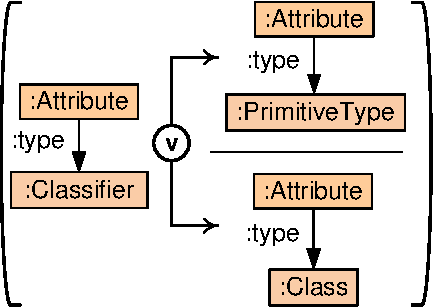
\includegraphics[width=.34\textwidth]{img/dc/constraints3.pdf}
}
The \code{type} edge is created by
rules \code{4:~TP2T} and \code{5:TC2T} in \cref{fig:rules}. The constraint on
the right is constructed by taking the atom with the \code{type} edge as the
premise and the disjunction of the embeddings of the atom into the right-hand-sides of both rules as the conclusion.
Analogously, the constraints for all other atoms $a \in Atoms(\TG_{S})$ over
source type graph $\TG_{S}$ in \cref{fig:mm} can be constructed.
\end{example}}


%%%%%%%%%%%%%%%%%%%%%%%%%%%%%%%%%%%%%%%%%%%%%%%%%%%%%%%%%%%%%%%%%%%%%%
%%%%%%%%%%%%%%%%%%%%%%%%%%%%%%%%%%%%%%%%%%%%%%%%%%%%%%%%%%%%%%%%%%%%%%
%%%%%%%%%%%%%%%%%%%%%%%%%%%%%%%%%%%%%%%%%%%%%%%%%%%%%%%%%%%%%%%%%%%%%%
%%%%%%%%%%%%%%%%%%%%%%%%%%%%%%%%%%%%%%%%%%%%%%%%%%%%%%%%%%%%%%%%%%%%%%
%%%%%%%%%%%%%%%%%%%%%%%%%%%%%%%%%%%%%%%%%%%%%%%%%%%%%%%%%%%%%%%%%%%%%%
%%%%%%%%%%%%%%%%%%%%%%%%%%%%%%%%%%%%%%%%%%%%%%%%%%%%%%%%%%%%%%%%%%%%%%
%%%%%%%%%%%%%%%%%%%%%%%%%%%%%%%%%%%%%%%%%%%%%%%%%%%%%%%%%%%%%%%%%%%%%%
%%%%%%%%%%%%%%%%%%%%%%%%%%%%%%%%%%%%%%%%%%%%%%%%%%%%%%%%%%%%%%%%%%%%%%
%%%%%%%%%%%%%%%%%%%%%%%%%%%%%%%%%%%%%%%%%%%%%%%%%%%%%%%%%%%%%%%%%%%%%%
%%%%%%%%%%%%%%%%%%%%%%%%%%%%%%%%%%%%%%%%%%%%%%%%%%%%%%%%%%%%%%%%%%%%%%
%%%%%%%%%%%%%%%%%%%%%%%%%%%%%%%%%%%%%%%%%%%%%%%%%%%%%%%%%%%%%%%%%%%%%%
%% app2.tex


% \newpage
% \section{Additional fragments to be possibly used in the paper}
% 
% ... now consider $\Lang_S \subseteq \Lang(TGG)\mid_{TG_S}$
% 
% This notion of domain-correctness can be achieved by showing $L(TGG)^T \subseteq L_T$.
% While this paper concentrates on the notion of domain-completeness, we define the task of providing a powerful method for showing the notion of domain-correctness as a challenge for future work and
% briefly describe how it can be handled with existing techniques.
% 
% 
% This paper presents a general method for validating and verifying this property in concrete application scenarios.
% We provide general results that ensure parts of the intermediate steps in general and 
% present in detail how the remaining parts can be solved including automated assistance by tool support.
% 
% This means that we have to show that $L_S \subseteq L(TGG)^S$.
% 
% \begin{math}
% \Lang_1=\Lang(TG_1,C_1) \Trans{Rest.} 
% \Lang_S=\restr{\Lang_1}{TG_S} \subseteq
% \Lang(TG_S,C_S) \subseteq \Lang(TG_S,TGG_S,C_{CT}) \subseteq \restr{\Lang(TGG)}{TG_S}
% \end{math}

% As in general,
% $L(TGG)^S \subseteq L(TR^S)$, we need to add constraints $C_2$ from $C_1'$ to
% $L(TR^S)$ leading to $L(TR^S+C_2)=\{G^S|\varnothing \xRightarrow{TR^{S*}} G^S, \forall c
% \in C_2.G^S \models c\}$ with $C_1' \implies C_2 \implies \varnothing$ until we
% hopefully get $L(TR^S+C_2) \subseteq L(TGG)^S$ without violating $L_S \subseteq
% L(TR^S+C_2)$ with the desired result $L_S \subseteq L(TGG)^S$ (cf. (1)).

% \subsection{Translation View of the Source Language}
% 
% Based on the concept of views in \cite{EEEP10}, a translation view of a language
% is defined as the restriction of the language to that subpart that is
% relevant for the model transformation.
% 
% \begin{definition}[Translation view]
% Given a language with constraints $L_{ATG,PC}$ and a triple type graph
% $ATG_S \leftarrow ATG_C \rightarrow ATG_T$ as a meta-model for the translation,
% then a translation view of that language is given by an injective morphism
% $v:ATG_S \rightarrow ATG$.
% \end{definition}
% 
% \begin{definition}[Restriction of models]
% Given a typed attributed graph $G$ with $G=(AG,t_{AG})$ typed over
% attributed type graph $ATG$ as a model and a translation view $v:ATG_S
% \rightarrow ATG$, then the restriction of the model $v^{<}(G)$
% with $v^{<}(G)=(AG_v,t_{AG_v})$
% is obtained by the pullback (1).
% \end{definition}
% 
% $
% 			\SelectTips{cm}{}
%     \xymatrix@R-4ex@C-4ex{ AG \ar[dd]_{t_{AG}} & & AG_v \ar[dd]^{t_{AG_v}}
%     \ar[ll] \\
%     			& (1) & \\
%                ATG & & ATG_S \ar[ll]^{v} }
% $
% 
% \begin{definition}[Restriction of constraints]
% Given a graph constraint $pc$ with $pc=((P, t_P) \xrightarrow{a} (C,
% t_C))$ typed over attributed type graph $ATG$ and a translation view $v:ATG_S
% \rightarrow ATG$, then the restriction of the constraint $v^{<}(pc)$ with
% $v^{<}(pc)=((P_v, t_{P_v}) \xrightarrow{a_v} (C_v,
% t_{C_v}))$ is obtained by pullbacks (1) and (2). Due to the universal
% property of pullback (2) with $v \circ t_{P_v}=t_P \circ p=t_C \circ a \circ p$,
% morphism $a_v$ exists such that $((P_v, t_{P_v}) \xrightarrow{a_v} (C_v,
% t_{C_v}))$ is a constraint over $ATG_S$.
% 
% The restriction of constraints is extended to the restriction $v^{<}(PC)$ of a
% set of constraints $PC$ with $v^{<}(PC)=\{v^{<}(pc) \mid pc \in PC\}$.
% \end{definition}
% 
% $
% 			\SelectTips{cm}{}
%     \xymatrix@R-4ex@C-4ex{
%     & P \ar[rr]^a \ar[dr]_{t_P} & & C \ar[dl]^{t_C} & \\
%     &  & ATG & & \\
%     & (1) & & (2) & \\
%     P_v \ar[uuur] \ar[rr]^{t_{P_v}} \ar@/_/[rrrr]_{a_v} & & ATG_S
%     \ar[uu]_{v} & & C_v \ar[uuul] \ar[ll]_{t_{C_v}} }
% $
% 
% \begin{definition}[Restriction of languages]
% Given a translation view $v:ATG_S \rightarrow ATG$ of language $L_{ATG,PC}$, the
% restriction of the language according to the view $v^{<}(L_{ATG,PC})$ is
% defined by the restriction of each graph and the restriction of each constraint
% of the language such that the restricted graphs fullfil the restricted
% constraints, i.e., $v^{<}(L_{ATG,PC})=\{v^{<}(G) \mid G \in L_{ATG,PC}, \forall c \in v^{<}(PC).G \models c\}$.
% \end{definition}
% 
% Note that in general, it is the fact that $v^{<}(G) \notin v^{<}(L_{ATG,PC})
% \text{ for some } G \in L_{ATG,PC}$.


%%%%%%%%%%%%%%%%%%%%%%%%%%%%%%%%%%%%%%%%%%%%%%%%%%%%%%%%%%%%%%%%%%%%%%
%%%%%%%%%%%%%%%%%%%%%%%%%%%%%%%%%%%%%%%%%%%%%%%%%%%%%%%%%%%%%%%%%%%%%%
%%%%%%%%%%%%%%%%%%%%%%%%%%%%%%%%%%%%%%%%%%%%%%%%%%%%%%%%%%%%%%%%%%%%%%
%%%%%%%%%%%%%%%%%%%%%%%%%%%%%%%%%%%%%%%%%%%%%%%%%%%%%%%%%%%%%%%%%%%%%%
%%%%%%%%%%%%%%%%%%%%%%%%%%%%%%%%%%%%%%%%%%%%%%%%%%%%%%%%%%%%%%%%%%%%%%
%%%%%%%%%%%%%%%%%%%%%%%%%%%%%%%%%%%%%%%%%%%%%%%%%%%%%%%%%%%%%%%%%%%%%%
%%%%%%%%%%%%%%%%%%%%%%%%%%%%%%%%%%%%%%%%%%%%%%%%%%%%%%%%%%%%%%%%%%%%%%
%%%%%%%%%%%%%%%%%%%%%%%%%%%%%%%%%%%%%%%%%%%%%%%%%%%%%%%%%%%%%%%%%%%%%%
%%%%%%%%%%%%%%%%%%%%%%%%%%%%%%%%%%%%%%%%%%%%%%%%%%%%%%%%%%%%%%%%%%%%%%
%%%%%%%%%%%%%%%%%%%%%%%%%%%%%%%%%%%%%%%%%%%%%%%%%%%%%%%%%%%%%%%%%%%%%%
%%%%%%%%%%%%%%%%%%%%%%%%%%%%%%%%%%%%%%%%%%%%%%%%%%%%%%%%%%%%%%%%%%%%%%
%% appendix.tex


For the rest of this section, we formalise the concepts of the proof idea of \cref{thm:C-extensionCompleteness} in order to finally prove \cref{thm:C-extensionCompleteness}.
We first show the equivalence of marking and transformation sequences with grammars for the case that the start graph is the empty graph in \cref{lem:equivalence-marking-emptySG} and that the start graph is an arbitrary graph in \cref{lem:equivalence-marking}.
Therefore, each graph that can be created via the rules of a given grammar $\GG$ can also be completely marked to $\True$ via the marking rules $m(\GG)$ of $\GG$ and vice versa.
%Given a graph $G$ with marking attributes, then by $(G^x \subseteq G)_{x \in \{\True, \False\}}$ we denote the subset of elements of $G$ (nodes, edges or attributes) that are annotated with a marking attribute of value $\True$ or $\False$, respectively.

\begin{lemma}[Equivalence of Marking and Transformation Sequence for empty Start Graph]
\label{lem:equivalence-marking-emptySG}
Let $\GG=(\varnothing,P)$ be a graph grammar with empty start graph $\varnothing$, a set $P$ of non-deleting rules and $m(\GG)$ be the set of derived marking rules of $\GG$. 
Let $G$ be a graph, then the following are equivalent for almost injective matches $m \in \morO$.
\begin{itemize}
	\item There exists a transformation $G \oplus \Att_G^\False \Trans{*} G \oplus \Att_{G_k}^\True \oplus \Att_{G \setminus G_k}^\False$ via marking rules $m(\GG)$.% with intermediate steps $(G'_i \Trans{(m_i,m(p_i))} G'_{i+1})$, where $m(p_i)=(L_i \xhookleftarrow{} K_i \xhookrightarrow{} R_i)$ and $\quotient{m_i}{L_i^{\False}}$ is type strict
	\item There exists a transformation $\varnothing \Trans{*} G_k$ via $P$ with injective embedding $f\colon G_k \to G$.% with intermediate steps $G_i \Trans{(m_i,p_i)} G_{i+1}$.
\envEndMarker
\end{itemize}
\end{lemma}

\begin{proof}
The proof is presented in \cref{sec-proofs:lem:equivalence-marking-emptySG}.
\end{proof}

% 
% 
% \noindent
% Using \cref{lem:equivalence-marking-emptySG} above, we now prove \cref{lem:equivalence-marking}.
% \\
% 
% \cref{lem:equivalence-marking} states the equivalence of marking rules
% $m(\GG)$ and the rules in $\GG$ in the sense that all graphs that can be
% completely marked to $\textbf{T}$ with rules $m(\GG)$ can also be created by
% the rules in $\GG$ and vice versa.

\begin{lemma}[Equivalence of Marking and Transformation Sequence]
\label{lem:equivalence-marking}
Let $\GG=(S,P)$ be a graph grammar with start graph $S$, a set $P$ of non-deleting rules and $m(\GG)$ be the set of derived marking rules of $\GG$. 
Let $G$ be a graph with inclusion $S \to G \in \M$, then the following are equivalent for almost injective matches $m \in \morO$.
\begin{itemize}
	\item There exists a transformation $G \oplus \Att_{S}^\True  \oplus \Att_{G\setminus S}^\False \Trans{*} G \oplus \Att_G^\True$ via marking rules $m(\GG)$.% with intermediate steps $G'_i \Trans{m_i,m(p_i)} G'_{i+1}$, where $m(p_i)=(L_i \xhookleftarrow{} K_i \xhookrightarrow{} R_i)$ and $\quotient{m_i}{L_i^{\False}}$ is type strict
	\item There exists a transformation $S \Trans{*} G$ via $P$.% with intermediate steps $G_i \Trans{p_i} G_{i+1}$.
\envEndMarker
\end{itemize}
\end{lemma}

\begin{proof}
The proof is presented in \cref{sec-proofs:lem:equivalence-marking}.
\end{proof}

\cref{def:bsplit} defines the binary split of a given graph $G$ into two sub-graphs which is extended to the general split of $G$ into its atoms $Atoms(G)$ in \cref{def:atomic-split} such that the gluing of the sub-graphs (atoms) yields $G$ again by \cref{lemma:union-subs,lemma:union-atoms}.
For proving \cref{lemma:union-atoms}, we show in \cref{lemma:split-nonatomic} that each non-atomic graph can be splitted.

%\vspace{1ex}
\parpic[r][r]{
$
\SelectTips{cm}{}
     \xymatrix@R-5ex@C-4ex{
     & \AG & \\
     \AG_1 \ar@{^{(}->}[ur]^{f'} & (1) & \AG_2 \ar@{_{(}->}[ul]_{g'} \\
     & \AG_0 \ar@{_{(}->}[ul]^{g} \ar@{^{(}->}[ur]_{f} &
     }
$
}
\vspace{-2ex}
\begin{definition}[Binary Split]
\label{def:bsplit}
\index{graph!binary split}
Let $\AG$ be a graph.
The set of \emph{binary splits} $BSplits(\AG)$ of $\AG$ into sub-graphs is given by co-spans of inclusions in \M:
\noindent
$
BSplits(\AG):= \{(\AG_1 \xhookrightarrow{f'} \AG \xhookleftarrow{g'} \AG_2) \mid $ 
(1) is  a pushout over inclusions $(f\colon \AG_0\xhookrightarrow{} \AG_2, g\colon \AG_0\xhookrightarrow{} \AG_1) \text{ with } f,f',g,g' \in \M, \AG \not\cong \AG_1, \AG\not\cong \AG_2\}$
%where $(\AG_1 \xhookrightarrow{f'_1} \AG \xhookleftarrow{g'_1} \AG_2) \sim (\AG'_1 \xhookrightarrow{f'_2} \AG \xhookleftarrow{g'_2} \AG'_2)$ if there exist isomorphisms $i_1\colon \AG_1 \to \AG'_1,i_2\colon \AG_2 \to \AG'_2$ and furthermore, $f'_1=f'_2 \circ i_1,g'_1=g'_2 \circ i_2$.
\envEndMarker
\end{definition}

\begin{corollary}[Gluing of Binary Split]
\label{lemma:union-subs}
Let $(\AG_1 \xhookrightarrow{f'} \AG \xhookleftarrow{g'} \AG_2) \in BSplits(\AG)$ be a binary split of $\AG$ into sub-graphs $\AG_1$ and $\AG_2$.
Then, there exist $\AG_0$ and a span of $\M$-morphisms $(\AG_1 \xhookleftarrow{g} \AG_0 \xhookrightarrow{f} \AG_2)$ such that (1) is a pushout.
\envEndMarker
\end{corollary}

% \begin{proof}
% Let $\AG=(G,D)$ and $(AG_i=(G_i,D))_{i \in \{0..2\}}$. By \cref{def:bsplit}, $(\AG,f',g')$ is a pushout over some inclusions $f\colon \AG_0
% \xhookrightarrow{} \AG_2$ and $g\colon \AG_0 \xhookrightarrow{} \AG_1$.
% Therefore, $f'(\AG_1) \cup g'(\AG_2) = \AG$. Furthermore, $f'_D=g'_D=id_D, f'_G(G_1)=G_1$ and $g'_G(G_2)=G_2$, i.e., $f'(\AG_1)=\AG_1$ and $g'(\AG_2)=\AG_2$. Therefore, $\AG_1 \cup \AG_2=\AG$.
% %\qed
% \end{proof}

\begin{lemma}[Binary Split of Non-Atomic Graphs]
\label{lemma:split-nonatomic}
Let $\AG$ be a graph that is not an atom, then $\AG$ can be splitted into sub-graphs $\AG_1$ and $\AG_2$ with $(\AG_1 \to \AG \gets \AG_2) \in BSplits(\AG)$.
\envEndMarker
\end{lemma}

\begin{proof}
We construct initial pushout (1) for $\id_\AG$ with $g' \in \M$.
Analogously, we construct initial pushout (2) for $g'$ with $f,f' \in \M$.
By \cref{sec-gt-M-adh,def:sec-gt-M-adh:hlr_props}, (2) is also a pullback, i.e., $g \in \M$ by $\M$-morphisms $g'$ are closed under pullbacks.
\begin{center}
$
\SelectTips{cm}{}
     \xymatrix@R-5ex@C-2ex{
     & & \AG & \\
     & \AG \ar[ur]^{\id_\AG} & (1) & \AG'' \ar[ul]_{} \\
     \AG_1 \ar[ur]^{f'} & (2) & \AG_2 \ar[ul]_{g'} \ar[ur]_{} & \\
     & \AG_0 \ar[ul]^{g} \ar[ur]_{f} & &
     }
$
\end{center}
Assumption $\AG$ is not an atom, \cref{def:atom} and $\M$-morphisms $f,g \in \M$ are closed under pushouts imply that there exists pushout (2) with $f,f',g,g' \in \M$ such that $\AG \not\cong \AG_1$ and $\AG \not\cong \AG_2$.
Thus according to \cref{def:bsplit}, there is $(\AG_1 \xhookrightarrow{f'} \AG \xhookleftarrow{g'} \AG_2) \in BSplits(\AG)$.
\end{proof}

Note that a graph $G$ may be splitted binary in different ways, possibly leading to several sets of atoms of $G$ in $Atoms(G)$.
However, for category $(\AGraphs_\ATGI,\M)$ all sets are isomorphic, i.e., only one set of atoms (decision path of binary splits) in $Atoms(G)$ need to be considered.

\begin{definition}[Atomic Split]
\label{def:atomic-split}
\index{graph!atomic split}
The \emph{set of atoms of a given graph $\AG$} is defined by $Atoms(\AG)$ as given below:
\newline
$
Atoms(\AG):= 
\begin{cases}
\{\{\AG\}\} & ,\AG \text{ is an atom} \\
\{A_1 \sqcup A_2 \mid (\AG_1 \xhookrightarrow{} \AG \xhookleftarrow{} \AG_2) \in BSplits(\AG), & ,\AG \text{ is not an atom} \\
A_1 \in Atoms(\AG_1),A_2 \in Atoms(\AG_2)\} & \hfill\envEndMarker
\end{cases}
$
\end{definition}

\parpic[r][r]{
$
\SelectTips{cm}{}
     \xymatrix@R-2ex@C-4ex{
     & PO_{k+1} & \\
     PO_k \ar@{^{(}->}[ur]^{f'_k} & (1) & a_{k+1} \ar@{_{(}->}[ul]_{g'_k} \\
     & G_k \ar@{_{(}->}[ul]^{g_k} \ar@{^{(}->}[ur]_{f_k} &
     }
$
}
\vspace{-2ex}
\begin{lemma}[Gluing of Atomic Split]
\label{lemma:union-atoms}
Let $G$ be a graph in $(\AGraphs_\ATGI,\M)$.
Then, there are atoms $(a_i)_{i \in \{1,\ldots,n\}} \in Atoms(G)$ and for all $(a_i)_{i \in \{1,\ldots,n\}} \in Atoms(G)$ there exist graphs $(G_j)_{1 \leq j \leq n-1}$ and pushouts $(PO_k +_{G_k} a_{k+1})_{k \in \{1,\ldots,n-1\}}$ with pushout objects $PO_{k+1}$ as depicted by pushout $(1)$ on the right with all morphisms in $\M$ and with $PO_1=a_1$ and induced morphisms $a_1 \trans{f'_1 \in \M} PO_2 \trans{f'_{n-1} \circ \ldots \circ f'_2 \in \M} PO_n \in \M$ and $a_{k+1} \trans{g'_k \in \M} PO_{k+1} \trans{f'_{n-1} \circ \ldots \circ f'_{k+1} \in \M} PO_n \in \M$ such that pushout object $PO_n$ is $G$.
\envEndMarker
\end{lemma}

\begin{proof}
Let $G$ be a graph.
\begin{description}
\item[Case ($G$ is an atom)] 
By construction \cref{def:atomic-split}, there is $\{G\} \in Atoms(G)=\{\{G\}\}$ with $n=1$, i.e., for all $(a_i)_{i \in \{1,\ldots,n\}} \in Atoms(G)$ the assumption holds with induced morphism $\id_G$.
\item[Case ($G$ is not an atom)]
By \cref{lemma:split-nonatomic}, there exists a binary split $(G_1 \trans{f'} G \transB{g'} G_2) \in BSplits(G)$.
By construction of binary splits in \cref{def:bsplit} with $G \not\cong G_1$, $G \not\cong G_2$ and injective $\M$-morphisms $f'$ and $g'$ it follows that $G_1$ and $G_2$ are smaller than $G$ on the graph part.
Therefore, analogously we can proceed with splitting $G_1$ and $G_2$ binary in $Atoms(G_1)$ and $Atoms(G_2)$ recursively and terminate in each decision path of binary splits when obtaining atoms.
Thus, there is $(a_i)_{i \in \{1,\ldots,n\}} \in Atoms(G)$.
Let $(a_i)_{i \in \{1,\ldots,n\}} \in Atoms(G)$ be the atoms of graph $G$.
By induction over the number $n$ of atoms:
\textbf{Basis.} For $n=2$, by construction there exists $(a_1 \trans{f'_1} G \transB{g'_1} a_2) \in BSplits(G)$ with $a_1,a_2$ being atoms, i.e., by \cref{lemma:union-subs} there exist $G_1$ and a span of $\M$-morphisms $(a_1 \transB{g_1} G_1 \trans{f_1} a_2)$ such that $(f'_1 \in \M,g'_1 \in \M)$ is a pushout over $(g_1,f_1)$ with induced morphisms $f'_1,g'_1 \in \M$ and with pushout object $PO_2=G$.
\textbf{Hypothesis.} There is $n$ such that the assumption holds.
\textbf{Step.} For $n+1$, note that in $(\AGraphs_\ATGI,\M)$, all decision paths of binary splits in $BSplits(G)$ lead to the same set of atoms $(a_i)_{i \in \{1,\ldots,n+1\}}$ up to isomorphism, i.e., we focus on that path where atoms are splitted from $G$ step-wise.
Let $G$ be binary splitted into $(G_1 \to G \gets a_{n+1}) \in BSplits(G)$ with atom $a_{n+1}$ and furthermore, let $(a_i)_{i \in \{1,\ldots,n\}} \in Atoms(G_1)$ and $(a_{n+1}) \in Atoms(a_{n+1})$.
By induction hypothesis, for $Atoms(G_1)$ there is pushout object $PO_n=G_1$ with induced morphisms in $\M$.
Analogously to the base case by \cref{lemma:union-subs}, for $(G_1 \trans{f'_n} G \transB{g'_n} a_{n+1}) \in BSplits(G)$ there is $G_n$ and pushout object $PO_{n+1}$ obtained by pushout $(f'_n \in \M,g'_n \in \M)=PO_n +_{G_n} a_{n+1}$ over $(g_n \in \M,f_n \in \M)$ with $PO_{n+1}=G$ and with induced morphisms in $\M$ by $\M$-composition with $f'_n \in \M$.
\end{description}
\end{proof}

Given a set of constraints $C$ that are designated for general satisfaction.
Then, \cref{lemma:closure-c-ext} states that for each atom $a$ of a graph $G$ which generally satisfies $C$, the extension of $a$ via $C$ is in $G$ again.
The result does not generally hold for constraints that are designated for initial satisfaction, since, atom $a$ may be extended at parts that are not covered by the satisfaction of the constraint potentially leading to extensions of $a$ that are not in G.

\begin{lemma}[Closure under $C$-Extensions of Atoms]
\label{lemma:closure-c-ext}
In $(\AGraphs_\ATGI,\M)$, let $C$ be a set of constraints that are designated for general satisfaction, $G \in \Lang(C)$ be a graph that generally satisfies $C$ and $a \in A \in Atoms(G)$ be an atom of $G$ with induced morphism $e\colon a \to G \in \M$ by \cref{lemma:union-atoms}.
Then, \emph{$G$ is closed under $C$-Extensions of $a$}, i.e., for all extensions $E \in Extensions(a,C)$ there is $a_E \in E$ with morphisms $e_1\colon a \to a_E \in \M, e_2\colon a_E \to G \in \M$ and $e=e_2 \circ e_1$.
\envEndMarker
\end{lemma}

\begin{proof}
The proof is presented in \cref{sec-proofs:lemma:closure-c-ext}.
\end{proof}

\cref{def:c-ext-set} extends the construction of $C$-extensions in \cref{def:C-extension} by defining the simultaneous extension of a set of graphs via a given set of constraints $C$.
This leads to the result in \cref{lem:union-ext-atoms} as an extension of \cref{lemma:union-atoms}.
Based on \cref{lemma:closure-c-ext}, \cref{lem:union-ext-atoms} states that given a graph $G$ which generally satisfies a given set of constraints $C$, then all simoultaneous extensions of the atoms of $G$ via $C$ contains a variant such that the gluing of the extended atoms yields graph $G$ again.

\begin{definition}[$C$-Extensions of Sets of Graphs]
\label{def:c-ext-set}
\index{$C$-extensions!sets of graphs}
Let $A$ be a set of graphs and $C$ be a set of constraints.
The set $SELECT_E(A,C)=\{f\colon A \to B \mid B=\bigcup_{a \in A}(Extensions(a,C)), \forall a \in A\colon f(a) \in Extensions(a,C)\}$ contains all functions $f$ that select for a given graph $a \in A$ an extension $E\in Extensions(a,C)$.
Let $f_E \in SELECT_E(A,C)$, then the set $SELECT_{a_E}(A,C,f_E)=\{f\colon A \to \bigcup_{E \in B}(E) \mid B=\bigcup_{a \in A}(Extensions(a,C)),\forall a \in A\colon f(a) \in f_E(a)\}$ contains all functions $f$ that select for a given graph $a \in A$ an extended graph $a_E \in f_E(a)$.
\envEndMarker 
\end{definition}

\begin{remark}
Note that for a graph $G$, the set of $C$-extensions $Extensions(G,C)$ may be infinite. Therefore, for a given set of graphs $A$, there may exists an infinite set of functions $SELECT_E(A,C)$.
Furthermore, a $C$-extension of a graph may be an infinite set of extended graphs. Therefore, for each selection $f_E \in SELECT_E(A,C)$, there may exists an infinite set of functions $SELECT_{a_E}(A,C,f_E)$.
\envEndMarker
\end{remark}

\begin{lemma}[Gluing of $C$-Extended Atoms]
\label{lem:union-ext-atoms}
In $(\AGraphs_\ATGI,\M)$, let $C$ be a set of constraints that are designated for general satisfaction, $G \in \Lang(C)$ be a graph that generally satisfies $C$ and $A=(a_i)_{i \in \{1,\ldots,n\}} \in Atoms(G)$ be the atoms of $G$.
Then, for all functions $f_E \in SELECT_E(A,C)$ that select a $C$-extension for each atom $a_i \in A$, there exists a function $f_{a_E} \in SELECT_{a_E}(A,C,f_E)$ that selects an extended atom for each atom $a_i \in A$ such that there exist graphs $(G^E_j)_{1 \leq j \leq n-1}$ and pushouts $(PO^E_k +_{G^E_k} f_{a_E}(a_{k+1}) = PO^E_{k+1})_{k \in \{1,\ldots,n-1\}}$ with pushout objects $PO^E_{k+1}$, all morphisms being in $\M$ and $PO^E_1=f_{a_E}(a_1)$ where (pushout object) $PO^E_n$ is $G$.
\envEndMarker 
\end{lemma}

\begin{proof}
The proof is presented in \cref{sec-proofs:lem:union-ext-atoms}.
\end{proof}

Note that in $(\AGraphs_\ATGI,\M)$, verifying domain completeness in \cref{thm:C-extensionCompleteness} via $C$-extension completeness in \cref{def:C-extensionCompleteness} is performed on the level of attributed graphs sharing the $\DSIG$-term algebra $T_\DSIG(X)$, since, effective atoms and their extensions share algebra $T_\DSIG(X)$ up to isomorphism by construction \cref{def:C-extension} with $e \in \M$ and \cref{sec-gt-M-adh,rem:sec-gt-M-adh:agraphs_atgi}.
In contrast to that, graphs of languages $\Lang(C)$ and $\Lang(\GG)$ may have concrete algebras with concrete values, in general (cf. general assumption of this section).
In order to close the algebra gap, in \cref{def:sec-dc-verification:instance_mor} we define instance morphisms $i\colon A \to B$ from attributed graphs $A$ with $\DSIG$-term algebra $T_\DSIG(X)$ to instance graphs $B$ with concrete algebras where concrete attribute values in $B$ are substituted by variables $x \in X$ in $A$ such that $i$ is an isomorphism on the graph part and injective for the data part of assigned attribute values.
Furthermore, we show that the verification of domain completeness on the term level does also hold for all (possibly infinitely many) instantiations to concrete values.
Therefore, given a set of productions $P$, in \cref{lem:atiti} we show that for each transformation $G \Trans{*} H$ via $P$ on the term level with instance morphism $i_H\colon H \to H'$ there is a corresponding transformation $G' \Trans{*} H'$ via $P$ with instance morphism $i_G\colon G \to G'$.
For proving \cref{lem:atiti}, based on the results in \cref{lem:comp_merge,lem:comp_e_mors} we first show in \cref{lem:ac_schema_sat_inst_mor} that a match satisfies an AC-schema if and only if the match extended by a given instance morphism satisfies the AC-schema.
\cref{lem:comp_merge} states that the successive merge over two morphisms is equivalent to the merge over the composition of both morphisms, i.e., in proofs for the satisfaction of AC-schemata, the merge over a composition of morphisms can be constructed step-wise (morphism by morphism successively).
For proving \cref{lem:comp_merge}, we additionally show the general results in \cref{lem:comp_o,lem:comp_epi,lem:m_adhesive_balanced,lem:pres_e_mor}.

\begin{definition}[Instance Morphism]
\label{def:sec-dc-verification:instance_mor}
\index{morphism!instance}
Let $DSIG=(S,OP)$ be a data signature.
In category $(\AGraphs_\ATGI,\M)$, \emph{a morphism $i\colon A \to B \in \E,\morO$ is an instance morphism}, if:
\begin{enumerate}
\item \label{item:sec-dc-verification:instance_mor:4}Attributed graph $A$ shares $\DSIG$-term algebra $T_\DSIG(X)$ with $X=(X_s)_{s \in S}$ being a family of infinite sets $X_s$ of variables for each sort $s \in S$,
\item \label{item:sec-dc-verification:instance_mor:5}attributed graph $B$ shares $\DSIG$-algebra $D_B$,
\item \label{item:sec-dc-verification:instance_mor:1}morphism $i$ is type strict,
\item \label{item:sec-dc-verification:instance_mor:2}all attribute values in $A$ are variables $x \in X$:$(\forall e \in E_j^A.t_j^A(e) \in X)_{j \in \{NA,EA\}}\}$, and
\item \label{item:sec-dc-verification:instance_mor:3}the data part of assigned attribute values is injective: $\forall d_1,d_2 \in D_A.(i_D(d_1)=i_D(d_2)) \wedge i_D(d_1) \in (t_{NA}^B(E_{NA}^B) \cup t_{EA}^B(E_{EA}^B)) \implies d_1=d_2$.
\envEndMarker
\end{enumerate}
\end{definition}

%#########################################################
\uncuttedversion{
Furthermore, we define the instances of an effective atom.
This is neccessary, since, effective atoms share the $\DSIG$-term algebra whereas graphs of a language (and its atoms) generally have algebras with concrete values which are considered as instances of terms (with variables).
In \cref{lemma:corr_atom_eatom}, we show that each effective atom $a \in EAtoms(C)$ is also an instance, i.e., $a \in \Inst(EAtoms(C))$.

\begin{definition}[Instance of Effective Atom]
\label{def:inst-effect-atom}
\index{atom!instance}
Given language $\Lang(C)$ over attributed type graph $\ATG$ and constraints $C$.
Let $a \in EAtoms(C)$ be an effective atom w.r.t. $\Lang(C)$ with morphism $f_a\colon a \to G \in \morO$ for some graph $G \in \Lang(C)$.% with $a=(G,D),\AG=(G',D')$.
The \emph{instance $\Inst_{f_a}(a)$ of atom $a$ w.r.t. $f_a$} is given by graph $O$ with extremal $\E$-$\M$ factorisation $m \circ e=f_a$ and $e\colon a \to O \in \E,m\colon O \to G \in \M$.
% $i_{f_a}(a)=a_I$ with
% $i_{f_a}(a):=(G'',D')$ and
% $G''=(f_a(V_G),f_a(E_G),V_D',f_a(E_{NA}),f_a(E_{EA}),(\quotient{s_i'}{f_a(E_i)},\quotient{t_i'}{f_a(E_i)})_{i
% \in \{G,NA,EA\}})$.
With $\Inst(a):=\{\Inst_{f_a}(a) \mid f_a\colon a \to G \in \morO,G \in \Lang(C)\}$ we denote the set of instances of atom $a$.
With $\Inst(EAtoms(C)):=\cup_{a \in EAtoms(C)}(\Inst(a))$ we denote the set of instances of effective atoms w.r.t. $\Lang(C)$.
\envEndMarker
\end{definition}

\begin{remark}
Note that for each (effective) atom $a$, an infinite set of morphisms $f_a\colon a \to G \in \morO$ with $G \in \Lang(C)$ may exist, i.e., each (effective) atom may have an infinite set of instances.
\envEndMarker
\end{remark}

\begin{lemma}[Correspondence of Atoms and Instances]
\label{lemma:corr_atom_eatom}
Given language $\Lang(C)$ over constraints $C$, and let $\AG \in EAtoms(C)$ be an effective atom w.r.t. $\Lang(C)$ with $i\colon \AG \to \AG' \in \M$ for some graph $\AG' \in \Lang(C)$.
Then, in category $(\AGraphs_\ATGI,\M)$ it holds that $\AG \in \Inst(EAtoms(C))$.
\envEndMarker
\end{lemma}

\begin{proof}
Let $f_a=i\colon \AG \to \AG' \in \M$ according to \cref{def:inst-effect-atom}, and $m \circ e=f_a$ be the extremal $\E$-$\M$ factorisation of $f_a$ with $e \in \E$ and $m \in \M$.
By $\M$-decomposition with $f_a,m \in \M$, it follows that $e \in \M$.
Therefore, according to \cref{sec-gt-M-adh,rem:sec-gt-M-adh:agraphs_atgi}, morphism $e$ is type strict, an isomorphism on the data part $e_D$ and injective on the graph part $e_G$.
Furthermore by $e \in \E$ and \cref{sec-gt-M-adh,rem:sec-gt-M-adh}, $e$ is an epimorphism, i.e., surjective, on the graph part $e_G$ implying further that $e$ is an isomorphism.
Thus, $\AG \in \Inst(EAtoms(C))$ up to isomorphism. 
\end{proof}


Analogously to \cref{def:inst-effect-atom}, we define the abstraction and instance of a graph.
This is neccessary, since, C-extension completeness verifies language inclusions on the level of attributed graphs sharing the term algebra with an infinite set of variables for each sort (abstract graphs).
In contrast to that, graphs of a language generally have algebras with concrete values, i.e., graphs of a language generally can be considered as instances of abstract graphs where variables are instantiated to concrete values.
Intuitively, the abstraction of an attributed graph $\AG^I=(G^I,D^I)$ with $DSIG$-algebra $D^I$ leads to an attributed graph $\AG=(G,T_{DSIG}(X))$ with a $DSIG$-term-algebra $T_{DSIG}(X)$ where concrete attribute values of $\AG^I$ are substituted by variables in $\AG$ such that all attributes with the same concrete value share the same variable and different concrete attribute values are substituted by different variables.
Therefore, each abstraction induces an instance morphism $i\colon \AG \to \AG^I$ that is an identity on the graph part and an isomorphism on the data part of assigned data values.
In order to obtain a unique instance morphism for each abstraction, the algebra $D^I$ must contain a designated abstraction element $*_s \in D_s^I$ for each sort $s$ to which unassigned variables are explicitly mapped. The unique evaluation of all other terms is given by the initiality of the term algebra $T_{DSIG}$.

\begin{definition}[Abstractable Graph]
\label{def:abstr-graph}
Let $DSIG=(S,OP)$ be a data signature. Let $\AG^I=(G^I,D^I)$ be an attributed graph with $DSIG$-algebra $D^I$. \emph{Graph $\AG^I$ is abstractable}, if $D^I$ contains a dedicated abstraction element $*_s \in D_s^I$ for each sort $s \in S$.
\envEndMarker
\end{definition}

In the following we define abstractions of graphs with concrete attribute values and instances of graphs.

\begin{definition}[Instance and Abstraction of Graphs]
\label{def:abstr-graphs}
Let $DSIG=(S,OP)$ be a data signature. Let $\AG^I=(G^I,D^I)$ be an abstractable attributed graph with $DSIG$-algebra $D^I$ and an abstraction element $*_s \in D_s^I$ for each $s \in S$.
\emph{The abstraction $\Abstr(\AG^I)$ of $\AG^I$} is defined by an instance morphism $\Abstr(\AG^I)=(i\colon \AG \to \AG^I)$
with $\AG=(G,D),D=T_{DSIG}(X),X=(X_s)_{s \in S}$ being a family of infinite sets $X_s$ of variables $(x^i_s)_{i \in \mathbb{N}}$ for each sort $s$ and $G=(V_{G}^I,V_{D},E_{G}^I,E_{NA}^I,E_{EA}^I,s_G^I,t_G^I,(s_j^I,t_j)_{j \in \{NA,EA\}})$ with $(\n{for all }e \in E_j^I \colon t_j(e) \in X)_{j \in \{NA,EA\}}\}$.
An instance morphism $i\colon \AG \to \AG^I$ is an attributed graph morphism without type refinements with $(i_{G,j})_{j \in \{V_G,E_G,E_{NA},E_{EA}\}}$ being identities, $\quotient{i_D}{t_{NA}(E_{NA}^I) \cup t_{EA}(E_{EA}^I)}$ and $\quotient{i_{G,V_D}}{t_{NA}(E_{NA}^I) \cup t_{EA}(E_{EA}^I)}$ being isomorphisms, and $(i_{D,s}(x_s^i)=*_s)_{s \in S}$ for all $x_s^i \in X \setminus (t_{NA}(E_{NA}^I) \cup t_{EA}(E_{EA}^I))$.
Let $A^I$ be a set of abstractable graphs. With $\Abstr(A^I)=\{\Abstr(\AG^I) \mid \AG^I \in A^I\}$ we denote the abstractions of graphs $A^I$.
Conversely, with $\Inst(\AG)=\{i\colon \AG \to \AG^I \mid i \n{ is an instance morphism} \}$ we denote the set of all instances of graph $\AG$.
\envEndMarker 
\end{definition}

\cref{def:compat-abstr} defines the situation in which the concrete values of the atomic sub-componenents of a graph are consistently abstracted to variables, i.e., identical (different) concrete values in different sub-components lead to identical (different) variables in their abstractions.

\begin{definition}[Compatible Abstraction of Atomic Sub-Components]
\label{def:compat-abstr}
Let $A^I=Atoms(\AG^I)$ be the atoms of an abstractable graph $\AG^I$.
\emph{The abstraction $\Abstr(A^I)$ of the atoms is compatible} with the abstraction $\Abstr(\AG^I)$ of $\AG^I$, if $\bigcup_{(i\colon A \to A^I) \in \Abstr(A^I)}(A)=\AG$ for $\Abstr(\AG^I)=(i\colon \AG \to \AG^I)$.
\envEndMarker 
\end{definition}
}
%####################################################################

\begin{lemma}[$\morO$-Morphisms are Closed Under De-Composition and Pushouts]
\label{lem:comp_o}
\label{lem:dec_o}
Let $f:\AG^1 \to \AG^2$, $g\colon \AG^2 \to \AG^3$ and $f'\colon \AG'^2 \to \AG^3$ be morphisms in $\AGraphs_{\ATGI}$.

\parpic[r][r]{
$
\SelectTips{cm}{}
     \xymatrix@R-5ex@C-5ex{
     AG^1 \ar@{->}[dd]^{} \ar@{->}[rr]^{f} & & AG^2 \ar@{->}[dd]^{g} \\
     & (1) & \\
     AG'^2 \ar@{->}[rr]^{f'} & & AG^3  
     }
$
}

\begin{enumerate}
  \item \label{item:lem:comp_o:1}If $f,g \in \morO$, then $g \circ f \in \morO$.
  \item Let $g \circ f = h$.
  \begin{enumerate}
    \item \label{item:lem:comp_o:2a}If $h \in \morO$, then $f \in \morO$.
    \item If $h \in \morO$ and graph part $f_S$ of $f$ is an isomorphism, then $g \in \morO$.
  \end{enumerate}
  \item For a given pushout (1), $f \in \morO$ implies $f' \in \morO$.\envEndMarkerB
\end{enumerate}
\end{lemma}

\begin{proof}
We proof the three facts as follows.
\begin{enumerate}
  \item The proof is given in \cite{DBLP:journals/tcs/GolasLEO12}, Thm. 7, item 7.
  \item
  \begin{enumerate}
    \item The proof is given in \cite{DBLP:journals/tcs/GolasLEO12}, Thm. 7, item 7.
    % With $g_S \circ f_S = h_S$,  $h_S$ being componentwise injective in $\cat{Sets}$ implies that $f_S$ is componentwise injective in $\cat{Sets}$, since, injective morphisms are closed under decomposition.
    % Therefore, $f \in \morO$.
    \item Let $f_S^{-1}\colon \AG^2 \to \AG^1$ be the inverse isomorphism of isomorphism $f_S$ with $f_S \circ f_S^{-1}=id_{\AG^2}$.
From $g_S \circ f_S = h_S$ we obtain $g_S \circ f_S \circ f_S^{-1} = h_S \circ f_S^{-1} \Leftrightarrow g_S \circ id_{\AG^2}=h_S \circ f_S^{-1} \Leftrightarrow g_S = h_S \circ f_S^{-1}$.
Since, $h_S, f_S^{-1}$ are componentwise injective in $\cat{Sets}$, it follows that $g_S$ is componentwise injective in $\cat{Sets}$, i.e., $g \in \morO$.
  \end{enumerate}
  \item Since (1) is a pushout, $f_S$ being componentwise injective in $\cat{Sets}$ implies that $f'_S$ is componentwise injective in $\cat{Sets}$ (cf. Fact 2.17, item 1 in \cite{Ehrig:2006:FAG:1121741}) and thus, $f' \in \morO$.
%  \qed
\end{enumerate}
\end{proof}

% \parpic[rf][r]{
% $
% \SelectTips{cm}{}
%      \xymatrix@R-3ex@C-3ex{
%      G_1 \ar@{->}[rr]^{h} \ar@{->}[dr]^{f} & & G_3 \\
%      & G_2 \ar@{->}[ur]^{g} &  
%      }
% $
% }
% \vspace{-2ex}
% \begin{lemma}[Decomposition of Isomorphisms]
% Let $f:G_1 \to G_2$, $g\colon G_2 \to G_3$ and $h\colon G_1 \to G_3$ be morphisms with $g \circ f = h$.
% \begin{enumerate*}
% \item If $h$ and $g$ are isomorphisms, then $f$ is an isomorphism.
% \item If $h$ and $f$ are isomorphisms, then $g$ is an isomorphism. 
% \end{enumerate*} 
% \envEndMarker
% \end{lemma}
% 
% \begin{proof}
% \begin{enumerate*}
% \item Let $g^{-1}\colon G_3 \to G_2$ be the inverse isomorphism of isomorphism $g$.
% Then, $g \circ f = h \Leftrightarrow g^{-1} \circ g \circ f = g^{-1} \circ h \Leftrightarrow id_{G_2} \circ f = g^{-1} \circ h \Leftrightarrow f = g^{-1} \circ h$.
% By the composition of isomorphisms $g^{-1}$ and $h$ it follows that $f$ is an isomorphism.
% \item Let $f^{-1}\colon G_2 \to G_1$ be the inverse isomorphism of isomorphism $f$.
% Then, $g \circ f = h \Leftrightarrow g \circ f \circ f^{-1}= h \circ f^{-1} \Leftrightarrow g \circ id_{G_1} = h \circ f^{-1} \Leftrightarrow g = h \circ f^{-1}$.
% By the composition of isomorphisms $h$ and $f^{-1}$ it follows that $g$ is an isomorphism.
% \end{enumerate*}
% \qed
% \end{proof}

% \begin{definition}[Merge$_{PO}$ over Morphism]
% Given a condition $\ac$ over $P$ and a morphism $b: P \rightarrow P'$, then based on \cref{def:merge morphism} $\Merge_{PO}(b,\ac)$ is a condition over $P'$ defined by
% \begin{itemize}
%   \item $\Merge_{PO}(b,\ac) = \exists(a',\Merge(b',\linebreak \ac'))$ if $\ac = \exists(a,\ac')$ and $(a',b',C')$ is a pushout over $(a,b,P)$,
%   \item $\Merge_{PO}(b,\ac) = \Merge(b,\ac)$, otherwise.
% \end{itemize}
% \envEndMarker
% \end{definition}
% 
% \begin{lemma}[Equivalence of $\Merge$ and $\Merge_{PO}$ Constructions]
% If b iso ($\morO$?) and $m \in \morO$, then $m \models \Merge(b,\ac) \Leftrightarrow m \models \Merge_{PO}(b,\ac)$.
% \envEndMarker
% \end{lemma}

%\vspace{-2ex}
\begin{lemma}[De-Composition of Pairs of Jointly Epimorphic Morphisms]\hfill
\label{lem:comp_epi}
\label{lem:decomp_epi}
\begin{center}
$
\SelectTips{cm}{}
     \xymatrix@R-5ex@C-3ex{
     G_0 \ar@{->}[dd]^{e} \ar@{->}[rr]^{e_2} & & G_1 \ar@{->}[dd]^{e_3} & & H \ar@{->}[ll]_{e_1} \\
     & (1) & & & \\
     G_2 \ar@{->}[rr]^{e_4} & & G & &  
     }
$
\end{center}
\begin{enumerate}
  \item Let $(e_1,e_2)$ and $(e_3,e_4)$ be pairs of jointly epimorphic morphisms and furthermore, (1) commutes.
        Then, $(e_3 \circ e_1,e_4)$ is a pair of jointly epimorphic morphisms.
  \item Let $(e_3 \circ e_1,e_4)$ be a pair of jointly epimorphic morphisms.
        Then, $(e_3,e_4)$ is a pair of jointly epimorphic morphisms.
  \item \label{lem:comp_epi:item:3} In the category $(\AGraphs_\ATGI,\M)$, let $(e_3,e_4)$ be a pair of jointly epimorphic morphisms, $e_4 \in \M$ and $e_1 \in \E$ be an extremal morphism w.r.t. $\M$.
        Then, $(e_3 \circ e_1,e_4)$ is a pair of jointly epimorphic morphisms.
  \item \label{lem:comp_epi:item:4} Let $(e_1,e_2)$ be jointly epimorphic and $e_3$ be an epimorphism.
        Then, $(e_3 \circ e_1,e_3 \circ e_2)$ is a pair of jointly epimorphic morphisms.
\envEndMarker 
\end{enumerate}
\end{lemma}

\begin{proof}
\begin{enumerate}
  \item We assume that (1) commutes and pairs $(e_1,e_2)$ and $(e_3,e_4)$ are jointly epimorphic.
        By the definition of jointly epimorphic morphisms, we have to show that for all graphs $G'$ and morphisms $f,g\colon G \to G'$ it holds that if $f \circ e_3 \circ e_1=g \circ e_3 \circ e_1$ $^{(*^1)}$ and $f \circ e_4=g \circ e_4$ $^{(*^2)}$, then $f=g$.
        Let $f,g\colon G \to G'$ be two morphisms with assumptions ($*^1$) and ($*^2$).
        Assumption ($*^2$) implies $f \circ e_4 \circ e=g \circ e_4 \circ e$.
        Since, (1) commutes it follows that $f \circ e_3 \circ e_2=g \circ e_3 \circ e_2$.
        By assumption ($*^1$) and $(e_1,e_2)$ being jointly epimorphic it follows that $f \circ e_3=g \circ e_3$.
        By assumption ($*^2$) and $(e_3,e_4)$ being jointly epimorphic it follows that $f=g$.
  \item We have to show for all morphisms $f,g$ that $f \circ e_3=g \circ e_3$ and $f \circ e_4=g \circ e_4$ implies $f=g$.
        Thus, $f \circ e_3=g \circ e_3 \implies f \circ e_3 \circ e_1=g \circ e_3 \circ e_1$.
        With $f \circ e_4=g \circ e_4$ it follows that $f=g$, since, $(e_3 \circ e_1,e_4)$ are jointly epimorphic.
  \item By assumption $e_4 \in \M$ and \cref{sec-gt-M-adh,rem:sec-gt-M-adh:agraphs_atgi}, $e_4$ is an isomorphism, i.e., an epimorphism, on the data part $e_{4,D}$.
        It remains to show that $(e_3 \circ e_1,e_4)$ are jointly epimorphic on the graph part.
        We assume the opposite.
        Then, there exists $g \in G$ with $g \not\in e_4(G_2)$ and $g \not\in e_3(e_1(H))$.
        The assumption that $(e_3,e_4)$ are jointly epimorphic implies that there exists $g' \in G_1$ with $e_3(g')=g$ but $g' \not\in e_1(H)$.
        Let $m \circ e'=e_1$ be the extremal $\E$-$\M$ factorisation of $e_1$  
        with $m\colon \ol{G_1} \to G_1 \in \M$.
        By the construction of the factorisation via the standard epi-mono factorisation on the graph structure part (cf. \cite{BEGG10}), it follows that $g' \not\in m(\ol{G_1})$ and therefore, $m$ is not an epi-(iso-)morphism.
        This contradicts with assumption $e_1 \in \E$ is extremal where $m \in \M$ implies that $m$ is an isomorphism (cf. \cref{def:EMFactorisation}).
  \item Given morphisms $g\colon G \to A$ and $h\colon G \to B$ with $g \circ e_3 \circ e_1=h \circ e_3 \circ e_1$ and $g \circ e_3 \circ e_2=h \circ e_3 \circ e_2$.
        By $(e_1,e_2)$ being jointly epimorphic, it follows that $g \circ e_3=h \circ e_3$ and $e_3$ being an epimorphism implies that $g=h$.
\end{enumerate}
\end{proof}

% \roundedYellowBox{
% \SelectTips{cm}{}
% $
% \xymatrix{
% P \ar[r]^a \ar[d]_b \ar@{}[dr]|{(1)}
% & C \ar[d]^{b'}
% \\
% P' \ar[r]_{a'}
% & C'
% }
% $
% }
% }

In general, it is not true that a monomorphism that is also an epimorphism is an isomorphism, since, the inverse morphism may not exist.
However, in $\M$-adhesive categories this assumption holds for a subclass $\M$ of monomorphisms as shown by \cref{lem:m_adhesive_balanced}.

\begin{lemma}[Relationship between $\M$-, Epi- and Iso-Morphisms in $\M$-adhesive Categories]
\label{lem:m_adhesive_balanced}
Given an $\M$-adhesive category $(\cat{C},\M)$, then any $\M$-morphism that is also an epimorphism is an isomorphism. 
\envEndMarker
\end{lemma}
\begin{proof}
The proof is based on the proof of Lemma 4.9 in \cite{Lack99adhesiveand} for adhesive categories.
Let (1) be a commuting diagram with epimorphism $m\colon A \to B \in \M$.
From $m$ being an epimorphism, it follows that (1) is a pushout, since, diagram (1) already commutes.
It remains to show the universal pushout property. 
For all morphisms $b_1,b_2\colon B \to \underline{B}$ with $b_1 \circ m=b_2 \circ m$ it follows that $b_1=b_2$ by the definition of epimorphisms.
Furthermore, there exists a morphism $\underline{b}=b_1=b_2$ with $\underline{b} \circ id_B=b_1 \circ id_B=b_2 \circ id_B=b_1=b_2$.
Moreover, $\underline{b}$ is unique.
Assume that there exists a morphism $\underline{b'}\colon B \to \underline{B}$ with $\underline{b'} \neq \underline{b}$ and $\underline{b'} \circ id_B=\underline{b'}=b_1=b_2=\underline{b}$ leading to a contradiction.

Since, (1) is a pushout along $\M$-morphism $m$, (1) is also a pullback (cf. Theorem 4.26, item 1 in \cite{Ehrig:2006:FAG:1121741}).
By the universal pullback property, there exists the inverse morphism $m^{-1}\colon B \to A$ with $m \circ m^{-1}=id_B$.
Furthermore, $m \circ id_A=id_B \circ m=m \circ m^{-1} \circ m$ and $m \in \M$ being a monomorphism by the definition of class $\M$ (cf. Def. 4.13 in \cite{Ehrig:2006:FAG:1121741}) implies $m^{-1} \circ m=id_A$.
\begin{center}
\begin{tikzpicture}[]
\fill (-3,1) node[inner sep=1pt] (Au) {$B$};
\fill (-2,0) node[inner sep=1pt] (A) {$A$};
\fill (0,0) node[inner sep=1pt] (B) {$B$};
\fill (0,-1) node[inner sep=1pt] (B'') {$B$};
\fill (-2,-1) node[inner sep=1pt] (B') {$B$};
\fill (1,-2) node[inner sep=1pt] (Bu) {$\underline{B}$};
\fill (-1,-.5) node[inner sep=1pt] (D1) {$(1)$};
%
{
\pgfsetarrowsend{latex}
\draw (B) -> node[right,inner sep=1pt]{$\scriptstyle{id_B}$} (B'');
\draw (B') -> node[below,inner sep=1pt]{$\scriptstyle{id_B}$} (B'');
\draw (Au) -> node[right,inner sep=5pt]{$\scriptstyle{m^{-1}}$} (A);
\draw (Au) edge[bend right=25] node[left,inner sep=1pt]{$\scriptstyle{id_B}$} (B');
\draw (Au) edge[bend left=25] node[right,inner sep=5pt]{$\scriptstyle{id_B}$} (B);
\draw (B'') -> node[above,inner sep=1pt]{$\scriptstyle{\underline{b}}$} (Bu);
\draw (B') edge[bend right=25] node[left,inner sep=5pt]{$\scriptstyle{b_1}$} (Bu);
\draw (B) edge[bend left=25] node[right,inner sep=1pt]{$\scriptstyle{b_2}$} (Bu);

\pgfsetarrows{right hook->>}
\draw (A) -> node[above,inner sep=1pt]{$\scriptstyle{m}$} (B);
\draw (A) -> node[left,inner sep=1pt]{$\scriptstyle{m}$} (B');
}
\end{tikzpicture}
\end{center}
%\qed
\end{proof}

\begin{lemma}[Preservation of Extremal Morphisms]\xqed{}
\label{lem:pres_e_mor}
\begin{minipage}{.68\textwidth}
Let $(\cat{C},\M)$ be an $\M$-adhesive category and $e \in \E$ be an extremal morphism with respect to $\M$ in $\cat{C}$.
Given diagram (1), if (1) commutes and morphisms $(a',e')$ are jointly epimorphic, then morphism $e'$ is an extremal morphism with respect to $\M$ in $\cat{C}$, i.e., $e' \in \E$.
\envEndMarker
\end{minipage}
\hfill
\begin{minipage}{0.3\textwidth}
\begin{tikzpicture}[]
\fill (0,0) node[inner sep=1pt] (P) {$P$};
\fill (0,-1) node[inner sep=1pt] (P') {$P'$};
\fill (-2,0) node[inner sep=1pt] (C) {$C$};
\fill (-2,-1) node[inner sep=1pt] (C') {$C'$};
\fill (-1,-.5) node[inner sep=1pt] (D1) {$(1)$};
%
{
\pgfsetarrowsend{latex}
\draw (P) -> node[above,inner sep=1pt]{$\scriptstyle{a}$} (C);
\draw (P') -> node[below,inner sep=1pt]{$\scriptstyle{a'}$} (C');
\draw (C) -> node[left,inner sep=3pt]{$\scriptstyle{e'}$} (C');

\pgfsetarrows{->>}
\draw (P) -> node[right,inner sep=3pt]{$\scriptstyle{e \in \E}$} (P');
}
\end{tikzpicture}
\end{minipage}
\end{lemma}

\begin{proof}
Let $(\cat{C},\M)$ be an $\M$-adhesive category, $e \in \E$, $e' \circ a=a' \circ e$ and $(a',e')$ be jointly epimorphic.
By the definition of extremal morphisms (cf. \cref{def:EMFactorisation}), morphism $e'$ is extremal ($e' \in \E$) if for all morphisms $c,c'$ with $c' \circ c=e'$ it is true that $c' \in \M$ implies $c'$ is an isomorphism.
Given a decomposition of $e'\colon C \to C'$ with morphisms $c\colon C \to \underline{C}$, $c'\colon \underline{C} \to C'$, $c' \circ c=e'$ and $c' \in \M$.
Since pullbacks exist along $M$-morphisms in $\cat{C}$ and $\M$-morphisms are closed under pullbacks (cf. Def. 4.9 in \cite{Ehrig:2006:FAG:1121741}), we can construct pullback $(PB)$ along $c' \in \M$ with $p' \in \M$.
By the universal pullback property and assumption $e' \circ a=c' \circ c \circ a=a' \circ e$, there exists morphism $p\colon P \to \underline{P}$ with $\underline{a} \circ p=c \circ a$ and $p' \circ p=e$.
Thus, $e \in \E$, $p' \circ p=e$ and $p' \in \M$ implies $p'$ is an isomorphism (cf. \cref{sec-gt-M-adh,def:EMFactorisation}).
It remains to show that $c'$ is an epimorphism.
By $c' \in \M$ and \cref{lem:m_adhesive_balanced} it would follow that $c'$ is an isomorphisms and thus, $e'$ is extremal.
Morphism $c'$ is an epimorphism means that for all morphisms $f,g\colon C' \to G$ it holds that $f \circ c'=g \circ c'$ implies $f=g$ (cf. Def. 2.13  in \cite{Ehrig:2006:FAG:1121741}).
Let $f \circ c'=g \circ c'$.
Therefore, $f \circ e'=f \circ c' \circ c=g \circ c' \circ c=g \circ e'$ $^{(*^1)}$.
Furthermore, $f \circ a'=f \circ a' \circ id_{P'}=f \circ a' \circ p' \circ p'^{-1}= f \circ c' \circ \underline{a} \circ p'^{-1}=g \circ c' \circ \underline{a} \circ p'^{-1}=g \circ a' \circ p' \circ p'^{-1}=g \circ a'$ $^{(*^2)}$ with $p'^{-1}$ being the inverse morphism of isomorphism $p'$.
Since, $(a',e')$ are jointly epimorphic, $(*^1)$ and $(*^2)$ implies $f=g$.
Therefore, $c'$ is an epimorphism and by \cref{lem:m_adhesive_balanced} $c'$ is an isomorphism and thus, $e' \in \E$.

\begin{center}
\begin{tikzpicture}[]
\fill (0,0) node[inner sep=1pt] (P) {$P$};
\fill (0,-3) node[inner sep=1pt] (P') {$P'$};
\fill (-4,0) node[inner sep=1pt] (C) {$C$};
\fill (-4,-3) node[inner sep=1pt] (C') {$C'$};
\fill (-3,-1.5) node[inner sep=1pt] (Cu) {$\underline{C}$};
\fill (-1,-1.5) node[inner sep=1pt] (Pu) {$\underline{P}$};
\fill (-2,-2.2) node[inner sep=1pt] (PB) {$(PB)$};
\fill (-6,-3) node[inner sep=1pt] (G) {$G$};
%
{
\pgfsetarrows{-latex}
\draw (P) -> node[above,inner sep=1pt]{$\scriptstyle{a}$} (C);
\draw (P') -> node[above,inner sep=1pt]{$\scriptstyle{a'}$} (C');
\draw (C) -> node[right,inner sep=1pt]{$\scriptstyle{c}$} (Cu);
\draw (P) -> node[left,inner sep=1pt]{$\scriptstyle{p}$} (Pu);
\draw (Pu) -> node[above,inner sep=1pt]{$\scriptstyle{\underline{a}}$} (Cu);
\draw (C) -> node[left,inner sep=3pt]{$\scriptstyle{e'}$} (C');
\draw (C'.north west) -> node[above,inner sep=1pt]{$\scriptstyle{f}$} (G.north east);
\draw (C'.south west) -> node[below,inner sep=1pt]{$\scriptstyle{g}$} (G.south east);

\pgfsetarrows{->>}
\draw (P) -> node[right,inner sep=3pt]{$\scriptstyle{e \in \E}$} (P');

\pgfsetarrows{right hook-latex}
\draw (Cu) -> node[right,inner sep=1pt]{$\scriptstyle{c'}$} (C');
\draw (Pu) -> node[left,inner sep=1pt]{$\scriptstyle{p'}$} (P');
}
\end{tikzpicture}
\end{center}
%\qed
\end{proof}

In general, the merge of a condition over two morphisms successively is not equivalent to the merge of the condition over the composition of both morphisms as illustrated by \cref{ex:merge_comp}.
\cref{lem:comp_merge} defines sufficient conditions under which the equivalence holds. 

\begin{example}[General Equivalence of Successive Merge and Merge over Composition]
\label{ex:merge_comp}
\cref{fig:merge_comp} illustrates the merge $\Merge(b_2 \circ b_1,\ac_P)$ of condition $\ac_P=\exists(a\colon P \to C,\true)$ over the composition of morphisms $b_1$ and $b_2$ as well as the merge $\Merge(b_2,\Merge(b_1,\ac_P))$ of $\ac_P$ over morphisms $b_1$ and $b_2$ successively.
The example serves as a counterexample for showing that the merge over a composition of two morphisms is not equivalent to the merge over both morphisms successively, in general.
For simplicity, the graphs in the example share no algebras and all nodes are of type $T0$.
The nodes are mapped to nodes of the same name along morphisms.
The merge over composition is constructed by the commuting outer diagram with morphisms $b' \in \morO$ and $a'' \in \M$ and results in condition $\exists(a''\colon P'' \to C'',\true)=\Merge(b_2 \circ b_1,\ac_P)$.
The successive merge results in condition $\false=\Merge(b_2,\Merge(b_1,\ac_P))$.
Diagram $(1)$ can be constructed for the first merge $\Merge(b_1,\ac_P)$ of $\ac_P$ over morphism $b_1$ but diagram $(2)$ does not exist for the subsequent merge over $b_2$, since, the merge construction requires that the morphism between graphs $C'$ and $C''$ must be an $\morO$-morphism where the nodes are mapped injectively (cf. \cref{def:merge morphism}) but no $\morO$-morphism can be found.
This results in condition $\false$ for the sucessive merge (cf. \cref{rem:mom}).
Thus, $\Merge(b_2,\Merge(b_1,\ac_P)) \not\equiv \Merge(b_2 \circ b_1,\ac_P)$, i.e., the merge of a condition over two morphisms successively is not equivalent to the merge of the condition over the composition of both morphisms, in general.
The same situation arises if $\ac_P$ is not in $\M$-normal form ($a \not\in \M$) and therefore, $a$ identifies elements that are not identified by $b_1$ but by $b_2$ and therefore, $(1)$ cannot be constructed resulting into $\Merge(b_1,\ac_P)=\false \Rightarrow \Merge(b_2,\Merge(b_1,\ac_P))=\false \not\equiv \Merge(b_2 \circ b_1,\ac_P)$ (cf. \cref{rem:mom}).
\envEndMarker

\begin{figure}[htb]
\begin{center}
\scalebox{1.0}{\begin{tikzpicture}[]

\node (P) [box]{ 
			\begin{tikzpicture}
			\node(title) {$P$}; 
			\node (P1) [below of=title, yshift=.5cm, anchor=west, normal, rectangle split parts=1] {1:T0};
			\end{tikzpicture}
};
\node (C) [right=of P, box, xshift=2cm]{ 
			\begin{tikzpicture}
			\node(title) {$C$}; 
			\node (C1) [below of=title, yshift=.5cm, anchor=west, normal, rectangle split parts=1] {1:T0};
			\end{tikzpicture}
};
\node (P') [below=of P, yshift=.5cm, box]{ 
			\begin{tikzpicture}
			\node(title) {$P'$}; 
			\node (P'1) [below of=title, yshift=.5cm, anchor=west, normal, rectangle split parts=1] {1:T0};
			\node (P'2) [right of=P'1, anchor=west, normal, rectangle split parts=1] {2:T0};       
			\end{tikzpicture}
};
\node (C') [below=of C, yshift=.5cm, box]{ 
			\begin{tikzpicture}
			\node(title) {$C'$}; 
			\node (C'1) [below of=title, yshift=.5cm, anchor=west, normal, rectangle split parts=1] {1:T0};
			\node (C'2) [right of=C'1, anchor=west, normal, rectangle split parts=1] {2:T0};
			\end{tikzpicture}
};
\node (P'') [below=of P', yshift=.5cm, box]{ 
			\begin{tikzpicture}
			\node(title) {$P''$}; 
			\node (P'1) [below of=title, yshift=.5cm, anchor=west, normal, rectangle split parts=1] {1,2:T0};
			\end{tikzpicture}
};
\node (C'') [below=of C', yshift=.5cm, box]{ 
			\begin{tikzpicture}
			\node(title) {$C''$}; 
			\node (C'1) [below of=title, yshift=.5cm, anchor=west, normal, rectangle split parts=1] {1,2:T0};
			\end{tikzpicture}
};

\fill (2.2,-.85) node[inner sep=1pt] (rect1) {$(1)$};
\fill (2.2,-2.8) node[inner sep=1pt] (rect2) {$(2)$};

{
\pgfsetarrowsend{latex}
\draw[thick] (P) ->node[left,inner sep=5pt]{$b_1$} (P');
\draw[thick] (P') ->node[left,inner sep=5pt]{$b_2$} (P'');

\pgfsetarrows{*-latex}
\draw[thick] (C) ->node[right,inner sep=5pt]{$b'_1 \in \morO$} (C');
\draw (C) edge[bend left=85] node[right,inner sep=5pt]{$b' \in \morO$} (C'');
\draw[thick] (C') edge[] node[right, inner sep=5pt]{$\nexists \in \morO$} (C'');

\pgfsetarrows{right hook-latex}
\draw[thick] (P) ->node[above,inner sep=1pt]{$a \in \M$} (C);
\draw[thick] (P') ->node[above,inner sep=1pt]{$a' \in \M$} (C');
\draw[thick] (P'') ->node[above,inner sep=1pt]{$a'' \in \M$} (C'');
}       

\end{tikzpicture}}
\caption{\label{fig:merge_comp}Counterexample for General Equivalence}
\end{center}
\end{figure}

\end{example}

\begin{lemma}[Equivalence of Successive Merge and Merge over Composition]
\label{lem:comp_merge}
In $(\AGraphs_\ATGI,\M)$, let $\ac_P$ be a condition over $P$ in $\M$-normal form.
Furthermore, let $b_1\colon P \to P'$ and $b_2\colon P' \to P''$ be morphisms from $P$ or
$P'$ to some $P'$ or $P''$, respectively.
Furthermore, let $b_1 \in \E$. 
It holds that $\Merge(b_2,Merge(b_1,\ac_P)) \equiv \Merge(b_2 \circ b_1,\ac_P)$.
\envEndMarker
\end{lemma}
\begin{center}
\begin{tikzpicture}[]
\fill (.5,1.7) node[inner sep=1pt] (P) {$P$};
\fill (0.5,.75) node[inner sep=1pt] (P') {$P'$};
\fill (0.5,-.2) node[inner sep=1pt] (P'') {$P''$};
\fill (-.1,1.7) node [isosceles triangle, fill=gray!25,draw,minimum width=0.4cm, inner sep=1pt] (t) {};
\fill (-.1,.75) node [isosceles triangle, fill=gray!25,draw,minimum width=0.4cm, inner sep=1pt] (t) {};
\fill (-.1,-.2) node [isosceles triangle, fill=gray!25,draw,minimum width=0.4cm, inner sep=1pt] (t) {};
\fill (-.6,1.7) node[inner sep=1pt] {$\ac_P$};
\fill (-1.45,.75) node[inner sep=1pt] {$\Merge(b_1,\ac_P)$};
\fill (-4,-.2) node[inner sep=1pt] {$\Merge(b_2 \circ b_1,\ac_P) \equiv \Merge(b_2, \Merge(b_1,\ac_P))$};
%
{
\pgfsetarrowsend{latex}
\draw (P') -> node[left,inner sep=1pt]{$\scriptstyle{b_2}$} (P'');

\pgfsetarrows{->>}
\draw (P) -> node[left,inner sep=1pt]{$\scriptstyle{b_1 \in \E}$} (P');
}
\end{tikzpicture}
\end{center}
\begin{proof}
The proof is presented in \cref{sec-proofs:lem:comp_merge}.
\end{proof}

\begin{lemma}[Composition of Extremal Morphisms]
\label{lem:comp_e_mors}
Let $(\cat{C},\M)$ be an $\M$-adhesive category and $e_1\colon A \to B,e_2\colon B \to C \in \E$ be extremal morphisms with respect to $\M$ in $\cat{C}$.
The composition $e_2 \circ e_1$ is also an extremal morphism with respect to $\M$ in $\cat{C}$ ($e_2 \circ e_1 \in \E$).
\envEndMarker
\end{lemma}
\begin{proof}
Let $e_1,e_2 \in \E$ and $m \circ f$ be a factorisation of $e_2 \circ e_1$ with $m \circ f=e_2 \circ e_1$ and $m \in \M$.
It remains to show that $m$ is an isomorphism (cf. \cref{def:EMFactorisation}).
We can construct pullback (1) along $m \in \M$ with $m_1 \in \M$, since, pullbacks exist along $\M$-morphisms in $\cat{C}$ and $\M$-morphisms are closed under pullbacks by definition (cf. Def. 4.13, item 2 in \cite{Ehrig:2006:FAG:1121741}).
By the universal pullback property we obtain morphism $f_1$ with $m_1 \circ f_1=e_1$.
Thus, the assumption $e_1 \in \E$ with $m_1 \in \M$ imply that $m_1$ is an isomorphism (cf. \cref{def:EMFactorisation}).
(1) being a pullback implies $e_2 \circ m_1=m \circ f_2 \stackrel{m_1\ iso}{\implies} e_2 \circ m_1 \circ m_1^{-1}=m \circ f_2 \circ m_1^{-1} \Leftrightarrow e_2 \circ id_B=m \circ f_2 \circ m_1^{-1} \Leftrightarrow e_2=m \circ f_2 \circ m_1^{-1}$.
Thus, the assumptions $e_2 \in \E$ and $m \in \M$ imply that $m$ is an isomorphism (cf. \cref{def:EMFactorisation}).
\begin{center}
\begin{tikzpicture}[]
\fill (0,0) node[inner sep=1pt] (A) {$A$};
\fill (3,0) node[inner sep=1pt] (B) {$B$};
\fill (6,0) node[inner sep=1pt] (C) {$C$};
\fill (3,2) node[inner sep=1pt] (B') {$\ol{B}$};
\fill (3,1) node[inner sep=1pt] (D) {$D$};
\fill (4,.7) node[inner sep=1pt] (1) {$(1)$};
\fill (2.35,.4) node[inner sep=1pt] (eq) {$(=)$};
%
{
\pgfsetarrows{-latex}
\draw (A) -> node[above,inner sep=1pt]{$\scriptstyle{f}$} (B');
\draw (D) -> node[right,inner sep=1pt]{$\scriptstyle{f_2}$} (B');
\draw (A) -> node[above,inner sep=1pt]{$\scriptstyle{f_1}$} (D);
\pgfsetarrows{->>}
\draw (A) -> node[above,inner sep=1pt]{$\scriptstyle{e_1 \in \E}$} (B);
\draw (B) -> node[above,inner sep=1pt]{$\scriptstyle{e_2 \in \E}$} (C);
\pgfsetarrows{right hook-latex}
\draw (B') -> node[right,inner sep=5pt]{$\scriptstyle{m \in \M}$} (C);
\draw (D) -> node[right,inner sep=1pt]{$\scriptstyle{m_1}$} (B);
}
\end{tikzpicture}
\end{center}
%\qed
\end{proof}

\cref{lem:ac_schema_sat_inst_mor} states that for a given match $m\colon P \to G$ and instance morphism $i\colon G \to G'$, $m$ satisfies the AC-schema $\ol{\ac}_P$ of a given condition $\ac_P$ in $\M$-normal form ($m \models \ol{\ac}_P$) if and only if $m$ extended by $i$ satisfies $\ol{\ac}_P$ ($i \circ m \models \ol{\ac}_P$).
For direction $i \circ m \models \ol{\ac}_P \Rightarrow m \models \ol{\ac}_P$, the restriction to conditions in $\M$-normal form becomes essential as illustrated by \cref{ex:schema_sat} leading to the restriction to application conditions in $\M$-normal form in \cref{lem:atiti}.

\begin{example}[AC-schema Satisfaction by Instance Morphisms for General Conditions]
\label{ex:schema_sat}
For category $(\AGraphs_\ATGI,\M)$, \cref{fig:schema_sat} illustrates that given a condition $\ac_P=\exists(a\colon P \to C,\true)$ that is not in $\M$-normal form, then it may be true that $i \circ m\models \ol{\ac}_P$ but $\neg(m \models \ol{\ac}_P)$.
\begin{figure}[htb]
\begin{center}
\scalebox{1.0}{\begin{tikzpicture}[]

\node (P) [box]{ 
			\begin{tikzpicture}
			\node(title) {$P$}; 
			\node (Item) [below=of title, anchor=west, yshift=1cm]
					{
							$\varnothing$
					};
			\end{tikzpicture}
};
\node (C) [right=of P, box, xshift=7.5cm]{ 
			\begin{tikzpicture}
			\node(title) {$C$}; 
			\node (Item) [below=of title, anchor=west, normal, yshift=.35cm]
					{
							1:T0
							\nodepart{second}
							$\begin{array}{l}
							value=x\\						
							\end{array}$
					};
			\end{tikzpicture}
};
\node (G) [below=of P, yshift=-1cm, box]{ 
			\begin{tikzpicture}
			\node(title) {$G$}; 
			\node (Item) [below=of title, anchor=west, normal, yshift=.35cm]
					{
							1:T0
							\nodepart{second}
							$\begin{array}{l}
							value=x					
							\end{array}$
					};
			\end{tikzpicture}
};
\node (P2) [right=of G, xshift=1cm, yshift=0cm, box]{ 
			\begin{tikzpicture}
			\node(title) {$P_2$}; 
			\node (Item) [below=of title, anchor=west, yshift=1cm]
					{
							$\varnothing$
					};
			\end{tikzpicture}
};
\node (C2) [right=of P2, xshift=1.7cm, box]{ 
			\begin{tikzpicture}
			\node(title) {$C_2$}; 
			\node (Item) [below=of title, anchor=west, normal, yshift=.35cm]
					{
							1:T0
							\nodepart{second}
							$\begin{array}{l}
							value=a					
							\end{array}$
					};
			\end{tikzpicture}
};
\node (G^I) [below=of G, box, yshift=-1cm]{ 
			\begin{tikzpicture}
			\node(title) {$G^I$}; 
						\node (Item) [below=of title, anchor=west, normal, yshift=.35cm]
					{
							1:T1
							\nodepart{second}
							$\begin{array}{l}
							value=1						
							\end{array}$
					};
			\end{tikzpicture}
};
\node (P3) [right=of G^I, xshift=1cm, yshift=0cm, box]{ 
			\begin{tikzpicture}
			\node(title) {$P_3$}; 
			\node (Item) [below=of title, anchor=west, yshift=1cm]
					{
							$\varnothing$
					};
			\end{tikzpicture}
};
\node (C3) [right=of P3, xshift=1.7cm, box]{ 
			\begin{tikzpicture}
			\node(title) {$C_3$}; 
			\node (Item) [below=of title, anchor=west, normal, yshift=.35cm]
					{
							1:T1
							\nodepart{second}
							$\begin{array}{l}
							value=1						
							\end{array}$
					};
			\end{tikzpicture}
};
\node (D1) [right=of P, xshift=3.5cm, yshift=-1.5cm]{(1)};
\node (D2) [right=of G^I, xshift=1.5cm, yshift=-.9cm]{(2)};
{
\pgfsetarrowsend{latex}
\draw[thick] (C3.south west) edge[bend left=15] node[fill=white,inner sep=5pt]{$\exists q' \in \M$} (G^I.south east);
\draw[thick] (C2.south west) edge[bend left=15] node[fill=white,inner sep=5pt,xshift=1cm]{$\nexists q \in \M$} (G.south east);
\draw[thick] (P) ->node[fill=white,inner sep=1pt]{$a\colon \begin{array}{l}
							x \mapsto x\\
							y \mapsto z\\
							z \mapsto z						
							\end{array}$} (C);

\pgfsetarrows{*-latex}
\draw[thick] (P) ->node[left,inner sep=1pt]{$m \in \morO\colon \begin{array}{l}
							x \mapsto a\\
							y \mapsto y\\
							z \mapsto z						
							\end{array}$} (G);
\draw[thick] (G) ->node[left,inner sep=1pt]{$i \in \morO\colon \begin{array}{l}
							a \mapsto 1\\
							x \mapsto 1\\
							y \mapsto 1\\
							z \mapsto 1						
							\end{array}$} (G^I);
\draw[thick] (C) ->node[left,inner sep=5pt]{$\nexists e'_1 \in \morO$} (C2);
\draw[thick] (C.south) edge[bend left=15] node[fill=white,inner sep=1pt]{$e'_2 \in \morO$} (C3.east);
\pgfsetarrows{->>}
\draw[thick] (P) ->node[fill=white,inner sep=5pt]{$e_1 \in \E$} (P2);
\draw[thick] (P2) ->node[fill=white,inner sep=1pt]{$e_2 \in \E$} (P3);
\pgfsetarrows{left hook-latex}
\draw[thick] (P2) ->node[above,inner sep=5pt]{$m_1 \in \M$} (G);
\draw[thick] (P3) ->node[above,inner sep=5pt]{$m_2 \in \M$} (G^I);
\pgfsetarrows{right hook-latex}
\draw[thick] (P2) ->node[above,inner sep=5pt]{$a_2 \in \M$} (C2);
\draw[thick] (P3) ->node[above,inner sep=5pt]{$a_3 \in \M$} (C3);
}       

\end{tikzpicture}}
\caption{\label{fig:schema_sat}AC-Schema Satisfaction by Instance Morphisms for General Conditions}
\end{center}
\end{figure}
Condition $\ac_P$ is not in $\M$-normal form, since, variables $y$ and $z$ are identified by $z$ along morphism $a\colon P \to C$, i.e., $a \not\in \M$ (cf. \cref{sec-gt-M-adh,rem:sec-gt-M-adh:agraphs_atgi}).
By \cref{sec-gt-gc,rem:sec-gc-gc:schemata}, $m \models \ol{\ac}_P$ means that $m_1 \models \Merge(e_1,\ac_P)$ and $i \circ m \models \ol{\ac}_P$ means that $m_2 \models \Merge(e_2 \circ e_1,\ac_P)$ for the extremal $\E$-$\M$ factorisations $m_1 \circ e_1=m$ and $m_2 \circ e_2 \circ e_1=i \circ m$.
Note that extremal $\E$-$\M$ factorisation $m_2 \circ e_2 \circ e_1$ of $i \circ m$ is obtained as follows: Given extremal $\E$-$\M$ factorisation $m_2 \circ e_2$ of $i \circ m_1$, then by \cref{lem:comp_e_mors} it follows that $e_2 \circ e_1 \in \E$ with $m_2 \circ e_2 \circ e_1=i \circ m$ and furthermore, by the uniqueness of factorisations (cf. \cref{sec-gt-M-adh,rem:sec-gt-M-adh:uniq_extr_EM_fact}), it follows that $m_2 \circ e_2 \circ e_1$ is the extremal $\E$-$\M$ factorisation of $i \circ m$.
Furthermore, $\Merge(e_1,\ac_P)=\false$, since, there does not exist $e'_1\colon C \to C_2$ such that (1) commutes, as, variables $y$ and $z$ in $P$ are identified by $z$ in $C$ along $a\colon P \to C$ but not by morphism $m$ and therefore, also not by $e_1$ (cf. \cref{sec-gt-gc,rem:mom}).
Contrarily, $\Merge(e_2 \circ e_1,\ac_P)=\exists(a_3\colon P_3 \to C_3,\true)$.
Thus, $m_2 \models \exists(a_3\colon P_3 \to C_3,\true)$ for morphism $q'\colon C_3 \to G^I \in \M$ with commuting (2) but $\neg(m_1 \models \false)$.
Consequently, $i \circ m\models \ol{\ac}_P$ but $\neg(m \models \ol{\ac}_P)$.
For negative conditions $\neg\ol{\ac}_P$ this means that $m \models \neg\ol{\ac}_P$ but $\neg(i \circ m \models \ol{\ac}_P)$.
For \cref{lem:atiti} this means that without the restriction to application conditions in $\M$-normal form, we obtain the undesired result that transformations on the term level via productions with negative application conditions not necessarily induce corresponding transformations on the level of concrete values, as, the application condition may be fulfilled by match $m$ but not by match $i \circ m$.
Independently from conditions not in $\M$-normal form, a similar situation may arise if we disregard \cref{def:sec-dc-verification:instance_mor,item:sec-dc-verification:instance_mor:3} for instance morphisms and focus on variable $x$ only in the example from above while neglecting variables $y$ and $z$, i.e., this time condition $\ac_P$ is in $\M$-normal form.
Therefore, the following example demonstrates the importance of \cref{item:sec-dc-verification:instance_mor:3} for the definition of instance morphisms.
Variable $x$ in $P$ is mapped to variable $a$ in $G$ along $m$.
Furthermore, variables $x$ and $a$ in $G$ are both mapped to $1$ in $G^I$ along $i$.
Note that this is only possible when explicitly disregarding \cref{def:sec-dc-verification:instance_mor,item:sec-dc-verification:instance_mor:3} for instance morphism $i$.
We can construct $(1)$ with $\Merge(e_1,\ac_P)=\exists(a_2\colon P_2 \to C_2,\true)$.
However, there does not exist $q\colon C_2 \to G$ such that $q \circ a_2=m_1$, since, this requires that variable $a$ in $C_2$ is simultaneously mapped to variable $a$ and $x$ in $G$ along $q$.
Thus, $\neg(m_1 \models \Merge(e_1,\ac_P))$ implying further that $\neg(m \models \ol{\ac}_P)$.
In contrast to that, we can construct $\Merge(e_2 \circ e_1,\ac_P)=\exists(a_3\colon P_3 \to C_3,\true)$ such that there is $q'\colon C_3 \to G^I$ with $q' \circ a_3=m_2$, i.e., $m_2 \models \Merge(e_2 \circ e_1,\ac_P)$ implying further that $i \circ m\models \ol{\ac}_P$.
Therefore, again $i \circ m\models \ol{\ac}_P$ but $\neg(m\models \ol{\ac}_P)$.
\envEndMarker
\end{example}

\begin{lemma}[AC-schema Satisfaction by Instance Morphisms]
\label{lem:ac_schema_sat_inst_mor}
Given a condition $\ac_P$ over $P$ in $\M$-normal form and its AC-schema $\ol{\ac}_P$.
Furthermore, given a match $m\colon P \to G \in \morO$ to some graph $G$ and an instance morphism $i\colon G \to G^I$.
Then, in $(\AGraphs_\ATGI,\M)$ it holds that $m \models \ol{\ac}_P$ if and only if $i \circ m \models \ol{ac}_P$.
\envEndMarker
\end{lemma}

\begin{proof}
The proof is presented in \cref{sec-proofs:lem:ac_schema_sat_inst_mor}.
\end{proof}

\begin{remark}
In \cref{lem:ac_schema_sat_inst_mor}, $i \circ m \models \ol{\ac}_P$ is well defined w.r.t. \cref{def:condition-satisfaction}, since, each instance morphism $i$ is in $\morO$ by definition.
\cref{lem:comp_o}, item 1 with $m \in \morO$ imply that $i \circ m \in \morO$.
\envEndMarker
\end{remark}

\begin{lemma}[Abstract transformations induce transformations of instances]
\label{lem:atiti}
Let $G_0 \Trans{*} G_n$ be a transformation via productions $P$ and almost injective matches $m \in \morO$ only, and with all application conditions in $\M$-normal form.
Let $i_n\colon G_n \to G_n^I$ be an instance morphism.
Then, in $(\AGraphs_\ATGI,\M)$ there exists a transformation $G_0^I \Trans{*} G_n^I$ via productions $P$ with instance morphism $i_0\colon G_0 \to G_0^I$.
\envEndMarker
\end{lemma}

\begin{proof}
Let $G_{n-1} \Trans{(\ol{p}_{n-1},m_{n-1})} G_n$ with pushout $(1)$ be the last direct transformation step of transformation $G_0 \Trans{*} G_n$ via production $\ol{p}_{n-1}=(p_{n-1} \in \M,\ac_{n-1})$ with application condition $\ac_{n-1}$ in $\M$-normal form and via match $m_{n-1} \in \morO$ by assumption.
Note that $g \in \M$ by $\M$-morphisms $p_{n-1}$ are closed under pushouts.
Therefore, $m_{n-1} \models \ol{\ac}_{n-1}$ by \cref{sec-gt-trafo,def:sec-gt-trafo:trafo}, with $\ol{\ac}_{n-1}$ being the AC-schema of $\ac_{n-1}$.
\begin{center}
\begin{tikzpicture}[]
\fill (0,0) node[inner sep=1pt] (G0) {$G_0$};
\fill (2.5,0) node[inner sep=1pt] (d) {$\ldots$};
\fill (6,0) node[inner sep=1pt] (Gn1) {$G_{n-1}$};
\fill (9,0) node[inner sep=1pt] (Gn) {$G_n$};
\fill (9,-2) node[inner sep=1pt] (GnI) {$G^I_n$};
\fill (6,-2) node[inner sep=1pt] (Gn1I) {$G^I_{n-1}$};
\fill (2.5,-2) node[inner sep=1pt] (dI) {$\ldots$};
\fill (0,-2) node[inner sep=1pt] (G0I) {$G^I_0$};
\fill (6,2) node[inner sep=1pt] (Ln1) {$L_{n-1}$};
\fill (5.2,2) node [isosceles triangle, fill=gray!25,draw,minimum width=0.4cm, inner sep=1pt] (t) {};
\fill (4.55,2) node[inner sep=1pt] {$\ol{\ac}_{n-1}$};
\fill (9,2) node[inner sep=1pt] (Rn1) {$R_{n-1}$};

\fill (7.5,1) node[inner sep=1pt] (1) {(1)};
\fill (7.5,-1) node[inner sep=1pt] (2) {(2)};

\fill (11,0) node[inner sep=1pt] (B) {B};
\fill (11,-2) node[inner sep=1pt] (C) {C};
\fill (10,-1) node[inner sep=1pt] (3) {(3)};
%
{
\pgfsetarrowsend{latex}
\draw[-implies,double equal sign distance] (G0) -> node[above,inner sep=1pt]{$\scriptstyle{(\ol{p}_0,m_0)}$} (d); 
\draw[-implies,double equal sign distance] (d) -> node[above,inner sep=1pt]{$\scriptstyle{(\ol{p}_{n-2},m_{n-2})}$} (Gn1);

\draw (Gn) -> node[right,inner sep=1pt]{$\scriptstyle{i_n}$} (GnI);
\draw (Ln1) -> node[right,inner sep=1pt]{$\scriptstyle{m_{n-1}}$} (Gn1);
\draw (Rn1) -> node[right,inner sep=1pt]{$\scriptstyle{m'_{n-1}}$} (Gn);

\draw[dotted] (Gn1) -> node[right,inner sep=1pt]{$\scriptstyle{i_{n-1}}$} (Gn1I);
\draw[dotted] (G0) -> node[right,inner sep=1pt]{$\scriptstyle{i_{0}}$} (G0I);

\draw[-implies,double equal sign distance,dotted] (G0I) -> node[above,inner sep=1pt]{$\scriptstyle{(\ol{p}_0,i_0 \circ m_0)}$} (dI);
\draw[-implies,double equal sign distance,dotted] (dI) -> node[above,inner sep=1pt]{$\scriptstyle{(\ol{p}_{n-2},i_{n-2} \circ m_{n-2})}$} (Gn1I);

\draw (B) -> node[left,inner sep=1pt]{$\scriptstyle{f}$} (C);

\draw (B) edge[->, bend right=25] node[above,inner sep=1pt]{$\scriptstyle{b^*}$} (Gn1);

\pgfsetarrows{right hook-latex}
\draw (Ln1) -> node[above,inner sep=1pt]{$\scriptstyle{p_{n-1} \in \M}$} (Rn1);
\draw (Gn1) -> node[above,inner sep=1pt]{$\scriptstyle{g \in \M}$} (Gn);
\draw[dotted] (Gn1I) -> node[above,inner sep=1pt]{$\scriptstyle{g' \in \M}$} (GnI);

\pgfsetarrows{left hook-latex}
\draw (B) -> node[above,inner sep=1pt]{$\scriptstyle{b \in \M}$} (Gn);
\draw (C) -> node[above,inner sep=1pt]{$\scriptstyle{c \in \M}$} (GnI);
}
\end{tikzpicture}
\end{center}
By \cref{def:sec-dc-verification:instance_mor}, instance morphism $i_n$ is in $\E$ and $\morO$ and therefore, graph part $i_{n,S}$ is an isomorphism in $(\AGraphs_\ATGI,\M)$.
Therefore, initial pushout $(3)$ for $i_n$ can be constructed with empty boundary graph $B$ on the graph part with data part $D_{G_n}$ and empty context graph $C$ on the graph part with data part $D_{G^I_n}$ where $b_S$ is the empty morphism on the graph part and $b_D$ is the identity on the data part (cf. Fact 10.7, Item 2, and Def. 10.5, Item 2, in \cite{Ehrig:2006:FAG:1121741}).
Note that $g \in \M$ implies that $g_D$ is an isomorphism with inverse isomorphism $g^{-1}_D$ by \cref{sec-gt-M-adh,rem:sec-gt-M-adh:agraphs_atgi}.
Thus, there is morphism $b^*\colon B \to G_{n-1}$ with $b^*_S$ being the empty morphism and $b^*_D=g^{-1}_D$ such that $g \circ b^*=b$.
Therefore, pushout complement $(g',i_{n-1})$ over $(g,i_n)$ exists leading to pushout $(2)$ (cf. \cref{sec-gt-M-adh,rem:sec-gt-M-adh}).
By pushout composition, $(1)+(2)$ is a pushout.
It remains to show that $i_{n-1}\colon G_{n-1} \to G^I_{n-1}$ is an instance morphism which would imply that $i_{n-1} \circ m_{n-1} \models \ol{\ac}_{n-1}$ by \cref{lem:ac_schema_sat_inst_mor} and therefore, $(1)+(2)$ is a direct transformation step $G^I_{n-1} \Trans{(\ol{p}_{n-1},i_{n-1} \circ m_{n-1})} G^I_n$ via production $\ol{p}_{n-1}$ and match $i_{n-1} \circ m_{n-1}$.
According to \cref{def:sec-dc-verification:instance_mor}:
\begin{enumerate}
  \item Morphism $i_{n-1} \in \morO$, since, $g \in \M \stackrel{\cref{sec-gt-M-adh,rem:sec-gt-M-adh:agraphs_atgi}}{\Rightarrow} g \in \morO$ and instance morphism $i_n \in \morO$ by \cref{def:sec-dc-verification:instance_mor} $\stackrel{\cref{lem:comp_o,item:lem:comp_o:1}}{\Rightarrow} i_n \circ g \in \morO$ $\stackrel{(2)}{\Rightarrow} g' \circ i_{n-1} \in \morO$ $\stackrel{\cref{lem:comp_o,item:lem:comp_o:2a}}{\Rightarrow} i_{n-1} \in \morO$,
  \item Morphism $i_{n-1} \in \E$, i.e., graph part $i_{n-1,S}$ is an epimorphism (surjective) in $(\AGraphs_\ATGI,\M)$:
  Assume that $i_{n-1,S}$ is not surjective, i.e., there is graph element $e \in G^I_{n-1}$ with $e \not\in i_{n-1,S}(G_{n-1})$.
  Furthermore, graph element $g'(e) \not\in i_n(G_n)$ by construction of pushouts in $(\AGraphs_\ATGI,\M)$ (cf. Fact 2.17 in \cite{Ehrig:2006:FAG:1121741}).
  This contradicts with assumption $i_n$ being an instance morphism, i.e., $i_n \in \E$ implying further that $i_{n,S}$ is an epimorphism (surjective) by \cref{def:sec-dc-verification:instance_mor}.
  Thus, $i_{n-1,S}$ is surjective implying further that $i_{n-1} \in \E$ in $(\AGraphs_\ATGI,\M)$,
  \item Graph $G_{n-1}$ shares $\DSIG$-term algebra by $g\colon G_{n-1} \to G_n \in \M$ being an isomorphism on the data part and $G_n$ shares $\DSIG$-term algebra by \cref{def:sec-dc-verification:instance_mor,item:sec-dc-verification:instance_mor:4} for instance morphism $i_n\colon G_n \to G^I_n$,
  \item Morphism $i_{n-1}$ is type strict: Morphism $g \in \M$ and instance morphism $i_n$ are type strict by \cref{def:sec-dc-verification:instance_mor,item:sec-dc-verification:instance_mor:1} (so $i_n \circ g$ is type strict).
  Assume that $i_{n-1}$ is not type strict, so $g' \circ i_{n-1}$ $\stackrel{(2)}{=} i_n \circ g$ is not type strict contradicting with $i_n \circ g$ is type strict.
  Thus, $i_{n-1}$ is type strict,
  \item All attribute values in $G_{n-1}$ are variables $x \in X$:
  Assume that $\exists e \in E^{G_{n-1}}_j.t^{G_{n-1}}_j(e) \not\in X,j \in \{NA,EA\}$.
  Note that $g_D(t^{G_{n-1}}_j(e))$ $\stackrel{g \in \morB}{=} t^{G_n}_j(g_{G,E_j}(e)) \in X$ by \cref{def:sec-dc-verification:instance_mor,item:sec-dc-verification:instance_mor:2} for instance morphism $i_n$, i.e., homomorphism $g_D$ maps a term $t \not\in X$ to a variable $x \in X$ which contradicts Fact B.16, Item 1, in \cite{Ehrig:2006:FAG:1121741} where $\ol{asg}$ is the unique homomorphism between two algebras for a given variable assignment that explicitly maps terms $t \not\in X$ to terms $t' \not\in X$ by Def. B.14 in \cite{Ehrig:2006:FAG:1121741}.
  Therefore, $\forall e \in E^{G_{n-1}}_j.t^{G_{n-1}}_j(e) \in X,j \in \{NA,EA\}$, and
  \item The data part of assigned attribute values is injective:
  Assume that $\exists d_1,d_2 \in D_{G_{n-1}}.(i_{n-1,D}(d_1)=i_{n-1,D}(d_2)) \wedge i_{n-1,D}(d_1) \in (t^{G^I_{n-1}}_{NA}(E^{G^I_{n-1}}_{NA}) \cup t^{G^I_{n-1}}_{EA}(E^{G^I_{n-1}}_{EA}))$ and where $d_1 \neq d_2$ implying further that $g'_D(i_{n-1,D}(d_1))=g'_D(i_{n-1,D}(d_2))$ $\stackrel{(2)}{\Rightarrow} i_{n,D}(g_D(d_1))=i_{n,D}(g_D(d_2))$ where $g_D(d_1) \in D_{G_n} \neq g_D(d_2) \in D_{G_n}$ by $g \in \M$ and therefore, $g_D$ being an isomorphism.
  Furthermore, $i_{n-1,D}(d_1) \in (t^{G^I_{n-1}}_{NA}(E^{G^I_{n-1}}_{NA}) \cup t^{G^I_{n-1}}_{EA}(E^{G^I_{n-1}}_{EA}))$ $\Rightarrow \text{for } j \in \{NA,EA\} \text{, } \exists e \in E^{G^I_{n-1}}_j.t^{G^I_{n-1}}_j(e)=i_{n-1,D}(d_1)$ $\Rightarrow t^{G^I_n}_j(g'_{G,E_j}(e)) \stackrel{g' \in \morB}{=} g'_D(t^{G^I_{n-1}}_j(e))=g'_D(i_{n-1,D}(d_1))$ $\stackrel{(2)}{=} i_{n,D}(g_D(d_1))$ $\Rightarrow i_{n,D}(g_D(d_1)) \in (t^{G^I_n}_{NA}(E^{G^I_n}_{NA}) \cup t^{G^I_n}_{EA}(E^{G^I_n}_{EA}))$.
  This contradicts \cref{def:sec-dc-verification:instance_mor,item:sec-dc-verification:instance_mor:3} for instance morphism $i_n$.
  Therefore, $\forall d_1,d_2 \in D_{G_{n-1}}.(i_{n-1,D}(d_1)=i_{n-1,D}(d_2)) \wedge i_{n-1,D}(d_1) \in (t_{NA}^{G^I_{n-1}}(E_{NA}^{G^I_{n-1}}) \cup t_{EA}^{G^I_{n-1}}(E_{EA}^{G^I_{n-1}})) \implies d_1=d_2$.
\end{enumerate}
Analogously, we can iterate over all direct transformation steps back to $G_0$ and yield a transformation $G_0^I \Trans{*} G_n^I$ via the same productions with instance morphism $i_0\colon G_0 \to G_0^I$.
\end{proof}

Effectively, \cref{lem:equivalence-marking-emptySG,lemma:union-atoms,lem:union-ext-atoms,lem:atiti} are used to prove the main result for verifying domain completeness in \cref{thm:C-extensionCompleteness}.

\uncuttedversion{
\cref{cor:abstr-ext-inst} closes the gap between abstract graphs used for verifying $C$-extension completeness and graphs with concrete attribute values.
For each $C$-extension $E$ of an abstract graph $\AG$, a $C$-extension $E^I$ can be constructed for any instance of $\AG$ such that if all graphs of $E$ can be constructed via a non-deleting grammar $\GG$, then also all graphs of $E^I$ can be constructed via $\GG$.
\begin{corollary}[Abstract C-Extensions induce C-Extensions with Instances]
\label{cor:abstr-ext-inst}
Let $\AG$ be a graph and $i\colon \AG \to \AG^I \in \Inst(\AG)$ be an instance of $\AG$. Let $C$ be a set of constraints and $\GG=(P,\varnothing)$ be a grammar with non-deleting productions $P$ and empty start graph.
Then, for each extension $E \in Extensions(\AG,C)$ with $E\ \subseteq \Lang(\GG,C)$ there exists an extension $E^I \in Extensions(\AG^I,C)$ with $E^I \subseteq \Lang(\GG,C)$.
\envEndMarker
\end{corollary}

\begin{proof}
Let $C$ be a set of constraints, $\GG=(P,\varnothing)$ be a grammar with non-deleting productions $P$ and empty start graph, $\AG$ be a graph with extension $E \in Extensions(\AG,C)$, $E \subseteq \Lang(\GG,C)$ and $i\colon \AG \to \AG^I \in \Inst(\AG)$.
For all extended graphs $(\AG_{E,i} \in E)_{i \in \{1\ldots\vert E\vert\}}$ of $\AG$ in $E$ the following holds by definition.
$\AG_{E,i}$ is obtained by a transformation $\AG \Trans{C^*} \AG_{E,i}$ via $C$ and furthermore, there exists a transformation $\varnothing \Trans{P^*} \AG_{E,i}$ via $P$ and $\AG_{E,i} \models C$.
By \cref{lem:atiti}, there exists a transformation $\AG^I \Trans{C^*} AG_{E,i}^I$ via $C$ with $i'\colon AG_{E,i} \to AG_{E,i}^I \in \Inst(AG_{E,i})$ and $\bigcup_{i \in \{1\ldots\vert E\vert\}}(\AG_{E,i}^I)=E^I \in Extensions(AG^I,C)$.
Furthermore, there exists a transformation $\varnothing \Trans{P^*} \AG_{E,i}^I$ via $P$ with $empty\colon \varnothing \to \varnothing \in \Inst(\varnothing)$.
By \cref{def:abstr-graphs} of instance morphism $i'\colon \AG_{E,i} \to \AG_{E,i}^I$ it follows that $\AG_{E,i}^I \models C$.
Thus, $E^I \subseteq \Lang(GG,C)$.
%\qed
\end{proof}
}

\uncuttedversion{
%\pagebreak
\begin{theorem}[Correctness of Construction of Constraints]
\label{th:correctness-constr}
Let $\GG=(\ATG,\SG,P)$ be a grammar typed over $\ATG$ with start graph $\SG$.
Let $C(\GG)$ be the set of constraints constructed from $\GG$. If $\SG \models
C(\GG)$, then $\Lang(\ATG,\GG) \subseteq \Lang(\ATG,C(\GG))$.\envEndMarker
\end{theorem}

\nn{
\begin{proof}
\end{proof}
}

\begin{remark}
In the presented model transformation framework, the constraints are
constructed from the grammar of source rules $TGG_S$ with an empty start
graph. Since, the constructed constraints $C(TGG_S)$ are all positive
and have at least one element in their premise, the start
graph trivially fulfills them ($\varnothing \models C(TGG_S)$).
\end{remark}

\begin{definition}[Covering]
Let $S$ be a set of graphs and let $\Lang$ be a language. \emph{$\Lang$ covers
$S$}, if for each graph $G \in S$ there exists a graph $G' \in \Lang$ with an
inclusion $i \colon G \xhookrightarrow{} G'$.
\end{definition}

\begin{theorem}[Completeness of Construction of Constraints]
\label{th:compl-constr}
Let $\Lang_2=\Lang(\ATG,\GG,C)$ be a language with grammar $\GG=(\ATG,\SG,P)$
and constraints $C$ typed over $\ATG$ where the rules $P$ are non-deleting. Let
$C(\GG)$ be the set of constraints constructed from $\GG$. If
$\Lang_2$ covers the set of effective atoms $EAtoms(\ATG)$ over $\ATG$ and $m(\GG)$ is C-conflict-free, then $\Lang_2$ is $C(\GG)$-extension complete and
$\Lang(\ATG,C \cup C(\GG)) \subseteq \Lang_2$.
\nn{Complete the theorem - at the moment the theorem is not working - a condition needs to be added that claims that all rules in \GG can be ordered such that the LHS of each rule is created jointly epi by a set of other rules except for the axioms, i.e., each rule in \GG is applicable at some point}
\end{theorem}

\nn{
\begin{proof}
\end{proof}
}

\nn{add figure of generated constraints for running example and argue that generated constraints are complete}

\begin{remark}
In view of \cref{th:correctness-constr}, with $C=\varnothing$ we get
$\Lang(\ATG,C(\GG)) \subseteq \Lang(\ATG,\GG)$.
\end{remark}
}
% \nn{DNF (dis. normal-form), nochmal nachschauen was passiert wenn max. 3 Statements hintereinander z.B. durch NAC}

\section{Limitations}
\label{sec-dc-general-lim}
\index{domain completeness!limitations}
The verification approach to solve the domain completeness problem in \cref{sec-dc-verification,thm:C-extensionCompleteness} is defined under the following assumptions which are likewise the limitations of the presented approach:

\begin{enumerate}
  \item The conditions for verifying domain completeness are only sufficient but not necessary.
  \item The approach is only applicable to graph grammars with empty start graphs.
  \item The approach is only applicable to graph grammars with non-deleting productions.
  \item The approach only involves constraints that are designated for general satisfaction while neglecting constraints that are designated for initial satisfaction.
  \item Constraints and application conditions need to be in $\M$-normal form.
  \item Termination of the approach requires an upper bound.
\end{enumerate}

\subsection{Conditions are Sufficient but not Necessary}

The conditions for verifying domain completeness in \cref{thm:C-extensionCompleteness} are only sufficient but not necessary.
Consider a grammar $\GG$ with duplicates of creating productions but for which the domain completeness holds.
The duplicates lead to a non-$C$-conflict-freeness of the marking rules $m(\GG)$ when claiming critical pairs of same rules and same matches.
Thus, the condition does not hold.
However, it is simple to exclude duplicates from the grammar.
For the confluence of marking rules we can find a similar example.

\subsection{Graph Grammars with Non-Empty Start Graph}

\begin{figure}[!tb]
\begin{center}
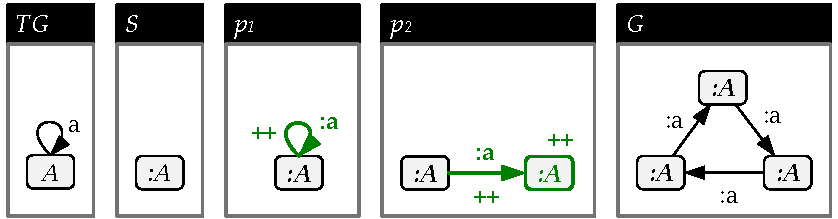
\includegraphics[width=.68\textwidth]{img/limitations/startgraph.pdf}
\end{center}
\caption{Limitation: Graph Grammar with Non-Empty Start Graph $S$}
\label{fig:sec-dc-general-lim:startgraph}
\end{figure}

We assume graph grammar $\GG=(S,P)$ typed over type graph $\TG$, with start graph $S$ and productions $P=\{p_1,p_2\}$ as depicted in \cref{fig:sec-dc-general-lim:startgraph}.
Furthermore, we assume that the set of domain constraints $C=\varnothing$ is empty.
By \cref{def:C-extensionCompleteness}, $\Lang(\GG)$ is $C$-extension complete and furthermore, by \cref{def:cf-marking-rules} $m(\GG)$ is $C$-conflict free, i.e., the conditions in \cref{sec-dc-verification,,thm:C-extensionCompleteness} hold.
However, for graph $G$ in \cref{fig:sec-dc-general-lim:startgraph} we obtain that $G \in \Lang(C)$ but $G \not\in \Lang(\GG)$.
Therefore the language inclusion does not hold although the conditions for domain completeness hold.
This is due to the gap between the declarative nature of graph constraints and the constructive nature of graph grammars.
Thus, the approach is only applicable to graph grammars with empty start graphs.

\subsection{Graph Grammars with Deleting Productions}

\begin{figure}[!tb]
\begin{center}
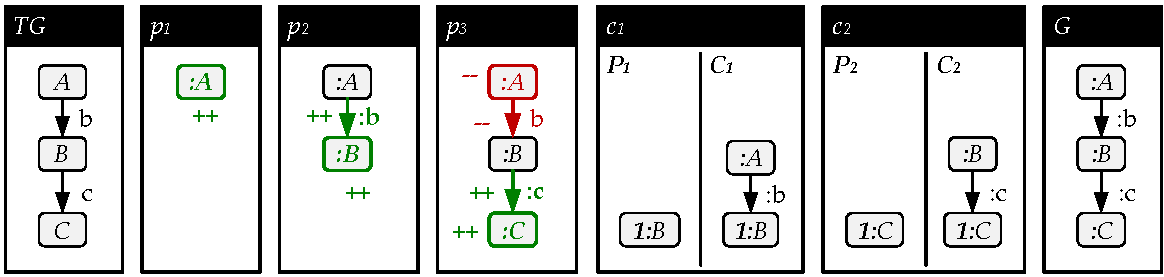
\includegraphics[width=\textwidth]{img/limitations/deleting.pdf}
\end{center}
\caption{Limitation: Graph Grammar with Deleting Production $p_3$}
\label{fig:sec-dc-general-lim:deleting}
\end{figure}

We assume graph grammar $\GG=(S=\varnothing,P)$ typed over type graph $\TG$ with the empty start graph and productions $P=\{p_1,p_2,p_3\}$ as depicted in \cref{fig:sec-dc-general-lim:deleting}.
Furthermore, we assume the set of domain constraints $C=\{c_1\colon P_1 \to C_1,c_2\colon P_2 \to C_2\}$ as depicted in \cref{fig:sec-dc-general-lim:deleting}.
Note that $\Lang(\GG)$ is $C$-extension complete by \cref{def:C-extensionCompleteness} and $m(\GG)$ seems to be $C$-conflict free by \cref{def:cf-marking-rules} when neglecting the deleting elements in production $p_3$.
Therefore, the conditions for domain completeness in \cref{sec-dc-verification,,thm:C-extensionCompleteness} seem to hold.
However, for graph $G$ in \cref{fig:sec-dc-general-lim:deleting} we obtain that $G \in \Lang(C)$ but $G \not\in \Lang(\GG)$.
Therefore the language inclusion does not hold.
This is due to the definition of marking rules which are only defined for non-deleting productions.
The example shows that elements that are deleted via productions cannot simply be neglected in marking rules.
Thus, the approach cannot be trivially extended to graph grammars with deleting productions and is only applicable to graph grammars with non-deleting productions.

\subsection{Initial \& General Satisfaction}
\begin{figure}[!tb]
\begin{center}
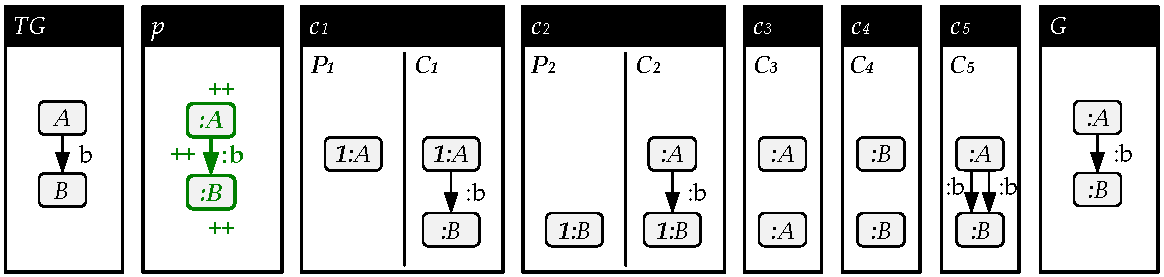
\includegraphics[width=\textwidth]{img/limitations/general.pdf}
\end{center}
\caption{Limitation: Initial \& General Satisfaction}
\label{fig:sec-dc-general-lim:igsat}
\end{figure}

Given type graph $\TG$, constraints $C_G=\{c_3,c_4\}$ designated for general satisfaction and $C_I=\{c_1,c_2\}$ designated for initial satisfaction, and grammar $\GG=(\varnothing,\{p\})$ where $c_1=\exists(P_1 \to C_1,\true),c_2=\exists(P_2 \to C_2,\true),c_3=\neg\exists(\varnothing \to C_3,\true),c_4=\neg\exists(\varnothing \to C_4,\true)$ and $c_5=\neg\exists(\varnothing \to C_5,\true)$.
Note that $\Lang(C)=\{G\} \subseteq \Lang(\GG)$, i.e., domain completeness holds.
However, constraints $c_1$ and $c_2$ are not used for $C$-extensions in \cref{sec-dc-verification,def:C-extension}, since, both are designated for initial satisfaction.
Therefore, $C$-extension completeness of $\Lang(\GG)$ does not hold, since, effective atoms $P_1,P_2$ and $G$ are not extended and cannot be created via grammar $\GG$.
The approach may be extended to also involve constraints that are designated for initial satisfaction in future work in order to handle situations from above appropriately.

\subsection{Constraints \& Application Conditions in $\M$-normal Form}

% \begin{figure}[!tb]
% \begin{center}
% 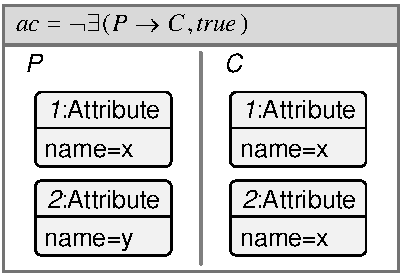
\includegraphics[width=.37\textwidth]{img/limitations/constraint.pdf}
% \end{center}
% \caption{Limitation: Application Condition not in $\M$-normal Form}
% \label{fig:sec-dc-general-lim:nf}
% \end{figure}

Note that for domain completeness, the graphs in $\Lang(C)$ and $\Lang(\GG)$ share the same ``concrete" algebra up to isomorphism by general assumption of \cref{sec-dc-verification}.
For verifying domain completeness $\Lang(C) \subseteq \Lang(\GG)$ in \cref{sec-dc-verification,,thm:C-extensionCompleteness}, we assume that all constraints $C$ and all application conditions in productions of graph grammar $\GG$ need to be in $\M$-normal form.
This is due to the fact that domain completeness is verified only once on the level of the $\DSIG$-term algebra for the data part and domain completeness for all concrete algebras can then be implied by \cref{sec-dc-verification,lem:ac_schema_sat_inst_mor,lem:atiti} but only when assuming the restriction to conditions in $\M$-normal form.
Therefore, a verification for each case of concrete algebras is not necessary.
\cref{sec-dc-verification,ex:schema_sat} depicts the necessity for conditions in $\M$-normal form and the full proof of \cref{sec-dc-verification,thm:C-extensionCompleteness} reveals all details.
In contrast to the presented approach, when performing the domain completeness verification directly on the concrete algebra for each case instead of a verification on the more abstract level of the term-algebra, then the restriction to conditions in $\M$-normal form may be loosened in future work.
Note that the restriction to conditions in $\M$-normal form forbids the definition of conditions that identify elements on the data part.
Therefore, constraints and application conditions of the following form cannot be expressed: ``For two or more nodes that have a node attribute $x$ each, it holds that all attributes $x$ share the same attribute value''.
However, we are confident that conditions in $\M$-normal form have enough expressive power for real-world scenarios.
% Consider the negative application condition $\ac=\neg\exists(P \to C,\true)$ in \cref{fig:sec-dc-general-lim:nf}.
% The NAC is not in $\M$-normal form, since, variables $x$ and $y$ are both mapped to $x$.
% A production in grammar $\GG$ that is equipped with this NAC is only applicable to graphs via matches, if the two matches \code{Attribute}s have different \code{name}s.
% However, the extension over atoms are only formed via $\M$-morphisms in \cref{def:C-extension} - Therefore, the construction does not lead to extension where both names share the same variable.
% Therefore, the language inclusion is verified on the abstract level of the term algebra, i.e., terms with variables, for attribute values, whereas graphs with concrete attributes values may identify different variables to the same concrete value, i.e., there may be transformation steps for graphs on the term level but not on the level for corresponding concrete graphs with concrete values.
% Thus, the conditions in \cref{sec-dc-verification} for the language inclusion holds although they may be graph that cannot be created via grammar $\GG$.
% More precisely, for a graph $P'=P[x \mapsto 1,y \mapsto 1]$ which is graph $P$ from \cref{fig:sec-dc-general-lim:nf} but where variables $x$ and $y$ are substituted by concrete value $1$ we obtain $P \models \ac$ but $P' \not\models \ac$.

\subsection{Termination Requires Upper Bound}

According to \cref{th:sec-dc-verification:term_dc}, we have to define an upper bound for the size of graphs in order to ensure termination of the approach.
In most cases, the verification terminates without restricting to an upper bound.
However, when restricting to an upper bound we could also check for all graphs up to the upper bound which satisfy the constraints in $C$ if they can be created via the rules in grammar $\GG$ for ensuring the validity of language inclusion $\Lang(C) \subseteq \Lang(\GG)$.
On the other hand, the verification via C-extension completeness in \cref{thm:C-extensionCompleteness} may be more efficient, since, not all graphs need to be checked but rather a small subset.


\section{Recursive Graph Constraints}
\label{sec-dc-general-rec}
\begin{figure}[!tb]
\begin{center}
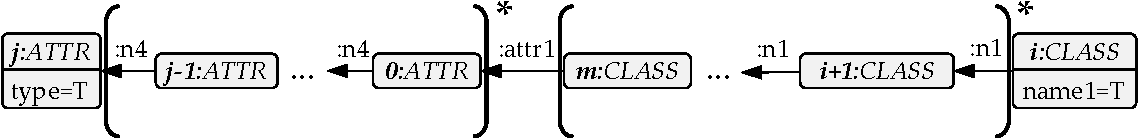
\includegraphics[width=.9\textwidth]{img/software_trans/rec_graph.pdf}
\end{center}
\caption{Language of Recursive Graph Schemata}
\label{fig:sec-compl-software-trans:rec_graph_lang}
\end{figure}

We introduce recursive conditions as a special class of infinite conditions and show that it is sufficient to check the components of the recursions only to verify domain completeness of the whole system.
Recursive conditions are infinite conditions that are given by the disjunction over the infinite set of graphs that are obtained from a start (premise) graph by repeating specific graph structures recursively.
In particular, this allows the definition of conditions over regular paths in abstract syntax graphs of source code.
\cref{fig:sec-compl-software-trans:rec_graph_lang} illustrates such a regular path expression defining that there is some path between an \code{ATTR}ibute $j$ of \code{type} $T$ and the \code{CLASS} $i$ with name $T$.
Concretely,
\begin{enumerate*}
\item[a)] either $j$ is directly connected to $i$ via edge \code{:attr1}, i.e., $j$ is the first attribute of class $i$, or
\item[b)] $j$ is the $j$th attribute of class $i$ and there are $j-1$ other attributes between both via \code{:n4} edges, or
\item[c)] $j$ is the first attribute of some other class $m$ and there are $m-i$ other classes between $i$ and $m$ via \code{:n1} edges, or
\item[d)] $j$ is the $j$th attribute of class $m$ and $m$ is the $m-i$th class defined behind class $i$.
\end{enumerate*}
Therefore, we want to describe an infinite set of graphs (paths) where the graph (path) structures that are enclosed by brackets with the Kleene star $*$ may be repeated recursively.
This allows the definition of the constraint ``Each attribute $j$ of type $T$ is the attribute of some class $m$ and moreover, for each such $j$ there is a class $i$ with name $T$ and either $i=m$ or $i$ is defined somewhere before $m$.'' - condensed ``For each attribute type that is used there is a corresponding class definition.''.
Such a constraint is rather an infinite constraint, i.e., the disjunction over all possible paths between $j$ and $i$. 
Thus, the motivation behind the notion of recursive conditions (constraints) is
\begin{enumerate*}
\item[a)] to have a notation for defining infinite graph conditions with recursively repeating graph structures,
\item[b)] and whose satisfiability is decidable,
\item[c)] the ability to involve infinite graph constraints in verifying domain completeness while in general, the verification of domain completeness for infinite constraints does not terminate, and
\item[d)] in particular, to use recursive graph constraints for specifying constraints over regular paths for the definition of abstract syntax graphs.
\end{enumerate*}
We introduce the notion of recursive graph schemata for the definition of infinite sets of graphs that are obtained from a start graph by the (recursively repeated) restricted application of productions via pre-defined matches between the productions.
 
\begin{definition}[Recursive Graph Schema]
\label{def:sec-compl-software-trans:rec_cond}
A \emph{recursive graph schema}\index{recursive graph schema} $\GS=(\GG,M,s_\GS,t_\GS)$ is given by
\begin{enumerate}
  \item a graph grammar $\GG=(S,P)$ with start graph $S$ and a set $P$ of productions $p=(L_p \transB{l_p} K_p \trans{r_p} R_p)$ with LHS $L_p$, gluing object $K_p$, RHS $R_p$ and $l_p,r_p \in \M$,
  \item a set $M$ of matches $m \in \M$ where
  \begin{enumerate}
    \item $m\colon L_p \to S$ from the LHS $L_p$ of some $p \in P$ to start graph $S$, or
    \item $m\colon L_p \to R_{p'}$ from the LHS $L_p$ of some $p \in P$ to the RHS $R_{p'}$ of some $p' \in P$, and
  \end{enumerate}
  \item source function $s_\GS\colon M \to P$ and target function $t_\GS\colon M \to (S \cup P)$ such that for all $m \in M$, $s_\GS(m\colon L_p \to A)=p$ and furthermore, $t_\GS(m\colon A \to S)=S$ or $t_\GS(m\colon A \to R_p)=p$ for some $p=(L_p \gets K_p \to R_p) \in P$.\envEndMarker
\end{enumerate} 
\end{definition}

\begin{remark}[Recursive Graph Schema]
Note that by function $s_\GS$, each match is mapped to exactly one rule as source (analogously, with $t_\GS$ for the target).
However, this does not restrict the expressiveness of recursive graph schemata.
Two rules $p_1\colon L \gets K_1 \to R_1,p_2\colon L \gets K_2 \to R_2$ with the same LHS $L$ and the same outgoing match $m\colon L \to A$ can be redefined by two rules $p_1,p'_2\colon L' \gets K_2 \to R_2$ with distinct LHSs $L \neq L'$ and distinct matches $m,m'\colon L' \to A$ by renaming the elements (nodes and edges) of $L$ resulting in $L'$ and without changing the semantics up to isomorphism.
This allows to define separate sources for $m,m'$ with $s_\GS(m)=p_1$ and $s_\GS(m')=p'_2$.
\envEndMarker
\end{remark}

\begin{figure}[!tb]
\begin{center}
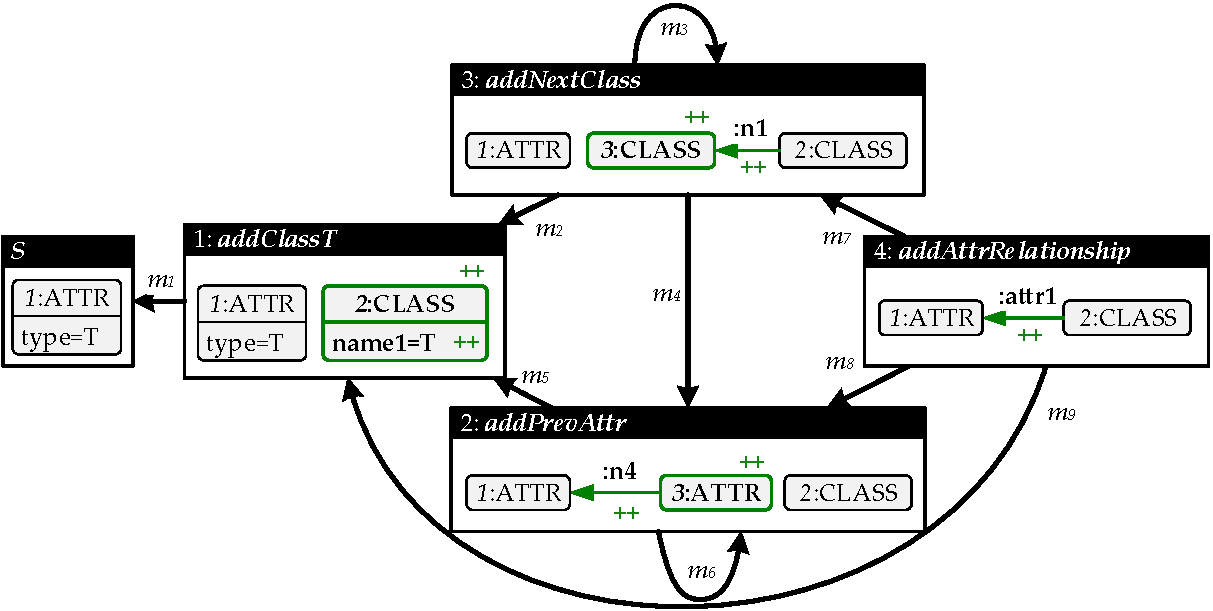
\includegraphics[width=.95\textwidth]{img/software_trans/graph_schema.pdf}
\begin{math}
m_1=(1 \mapsto 1); m_2=(1 \mapsto 1,2 \mapsto 2); m_3=(1 \mapsto 1,2 \mapsto 3); m_4=(1 \mapsto 3,2 \mapsto 2);m_5=(1 \mapsto 1,2 \mapsto 2);m_6=(1 \mapsto 3,2 \mapsto 2);m_7=(1 \mapsto 1,2 \mapsto 3);m_8=(1 \mapsto 3,2 \mapsto 2);m_9=(1 \mapsto 1,2 \mapsto 2)
\end{math}
\begin{math}
s_\GS(m_1)=\code{1:addClassT};s_\GS(m_2)=s_\GS(m_3)=s_\GS(m_4)=\code{3:addNextClass};s_\GS(m_5)=s_\GS(m_6)=\code{2:addPrevAttr};s_\GS(m_7)=s_\GS(m_8)=s_\GS(m_9)=\code{4:addAttrRelationship};
\end{math}
\begin{math}
t_\GS(m_1)=S;t_\GS(m_2)=t_\GS(m_5)=t_\GS(m_9)=\code{1:addClassT};t_\GS(m_3)=t_\GS(m_7)=\code{3:addNextClass};t_\GS(m_4)=t_\GS(m_6)=t_\GS(m_8)=\code{2:addPrevAttr};
\end{math}
\end{center}
\caption{Recursive Graph Schema}
\label{fig:sec-compl-software-trans:rec_graph}
\end{figure}

\begin{example}[Recursive Graph Schema]
\label{ex:sec-compl-software-trans:rec_schema}
\cref{fig:sec-compl-software-trans:rec_graph} illustrates a recursive graph schema with start graph $S$, productions $\{1 \ldots 4\}$, matches $\{m_1 \ldots m_9\}$ and source (target) function $s_\GS$ ($t_\GS$) which defines the infinite set of graphs that are presented in \cref{fig:sec-compl-software-trans:rec_graph_lang}.
From start graph $S$ we obtain the graph with the corresponding \code{CLASS} of name $T$ and edge \code{:attr1} by applying rules \code{1} and \code{4} via matches $m_1$ and $m_9$ successively.
Analogously, we may obtain bigger graphs beginning with $S$ by (repeatedly) applying rules \code{2} and \code{3} via corresponding matches $m_2 \ldots m_6$ before applying rule \code{4}.
Note that cycles of match morphisms define graph structures that may be repeated recursively.
The repeated application of rule~\code{3} via match $m_3$ allows the repeated addition of classes whereas rule~\code{2} together with match $m_6$ allows the repeated addition of attributes.
\envEndMarker
\end{example}

We define the precise semantics of a recursive graph schema $\GS$ by its graph language which is induced by terminating recursive transformation sequences over the schema starting at start graph $S$.
A recursive transformation sequence is given by a path of matches $M$ in $\GS$ and a corresponding sequence of recursive transformation steps where the match of each step is restricted by the co-match of the previous step.
The sequence is terminating in the sense that there are no matches defined in $M$ for extending the sequence.
A path of matches $M$ in $\GS$ is given by a sequence of matches $(m_i \in M)_{i \in I}$ with $s_\GS(m_i)=t_\GS(m_{i+1})$, for all $i \in I$.

\begin{definition}[Cyclic \& Terminating Match-Path]
\label{def:sec-compl-software-trans:c_t_match-path}
Let $\GS=((S,P),M,s_\GS,t_\GS)$ be a recursive graph schema.
A \emph{match-path in $\GS$}\index{match-path} is a sequence of $n>0$ matches $(m_i \in M)_{i \in I},I=\{1 \ldots n\}$ with $s_\GS(m_i)=t_\GS(m_{i+1})$, for all $i \in I$.
A match-path with $n$ matches is \emph{terminating}\index{match-path!terminating}, if there does not exist a match $m \in M$ with $t_\GS(m)=s_\GS(m_n)$.
A match-path is \emph{acyclic}\index{match-path!acyclic}, if for all $i,j \in I$ it is true that $i \neq j$ implies $s_\GS(m_i) \neq s_\GS(m_j)$.
Otherwise, the match-path is \emph{cyclic}\index{match-path!cyclic}.
A match-path of $n$ matches \emph{starts (ends)}\index{match-path!starts in}\index{match-path!ends in} in $A$, if $t_\GS(m_1)=A$ ($s_\GS(m_n)=A$).
With $\Paths_A(\GS)$ we denote \emph{the set of all match-paths in $\GS$ that start in $A$} and with $\Paths_{A,B}(\GS)$ we denote \emph{the set of all match-paths in $\GS$ that start in $A$ and end $B$}\index{match-path!set of paths}.
A \emph{match-cycle is some match-path $\paths \in \Paths_{A,A}(\GS)$}\index{match-path!match-cycle}.
A \emph{match-cycle $\paths \in \Paths_{A,A}(\GS)$ is reachable from match-path $(m_i)_{i \in \{1\ldots n\}}$}\index{match-path!match-cycle!reachable}, if there is some $i$ with $s_\GS(m_i)=A$ or $t_\GS(m_i)=A$.
\envEndMarker
\end{definition}

\begin{example}[Match-Path]
Given the recursive graph schema $\GS$ in \cref{fig:sec-compl-software-trans:rec_graph}.
For example, $m=(m_1,m_5,m_6,m_8)$ is a match path with four matches - the source of each match coincides with the target of its successive match.
Furthermore, $m$ is terminating (there is no match with rule \code{4:} as target), $m$ is cyclic ($s_\GS(m_5)=s_\GS(m_6)$) and $m \in \Paths_{S,\code{4:}}(\GS)$.
The same path without match $m_6$ is acyclic.
Match-path $(m_6) \in \Paths_{\code{2:},\code{2:}}(\GS)$ is a match-cycle that is reachable from $m$.
\envEndMarker
\end{example}

\begin{proposition}[(De)-Composition of Acyclic Match-Paths]
\label{prop:sec-compl-software-trans:decomp_acyclic_match-paths}
Given two match-paths $\paths_1=(m_{1,i})_{i \in \{1\ldots n\}}$ and $\paths_2=(m_{2,i})_{i \in \{1\ldots m\}}$ together with their merged match-path $\paths_3=(m_{1,1}\ldots m_{1,n},m_{2,1}\ldots m_{2,m})$.
If $\paths_3$ is acyclic, then $\paths_1$ and $\paths_2$ are acyclic \emph{(Decomposition)}\index{match-path!acyclic!decomposition}.
However conversely, if $\paths_1$ and $\paths_2$ are acyclic, then $\paths_3$ is not necessarily acyclic but may be cyclic \emph{(Composition)}\index{match-path!acyclic!composition}.
\envEndMarker
\end{proposition}

\begin{proof}
``Decomposition'': Assume that $\paths_i$ is cyclic for $i \in \{1,2\}$.
Then, the composition $\paths_3$ is cyclic by definition contradicting with the assumption that $\paths_3$ is acyclic.
``Composition'': The counterexample is as follows: Let $n=m=1$ and $m_{1,1}=m_{2,1}$ be a reflexive match, i.e., $s_\GS(m_{1,1})=t_\GS(m_{1,1})=s_\GS(m_{2,1})=t_\GS(m_{2,1})$.
Match-paths $\paths_1$ and $\paths_2$ are acyclic, respectively, but the composition $\paths_3=(m_{1,1},m_{2,1})$ is cyclic.
\end{proof}

\begin{definition}[Recursive Transformation]
\label{def:sec-compl-software-trans:rec_trafo}
Let $\GS=((S,P),M,s_\GS,t_\GS)$ be a recursive graph schema.
A \emph{recursive transformation step}\index{recursive transformation!step} $G \Trans{(p,m,n)}_{\GS,n'} G'$ from $G$ to $G'$ via production $p=(L_p \transB{l_p} K_p \trans{r_p} R_p), p \in P$, match $m\colon L_p \to A,m \in M$ and morphism $n\colon A \to G,n \in \M$ is defined by a direct transformation $G \Trans{(p,n \circ m)} G'$ via $p$ and $n \circ m$ with pushouts $(1),(2)$ and co-match $n'\colon R_p \to G' \in \M$.
A \emph{recursive transformation sequence}\index{recursive transformation!sequence} w.r.t. a given match-path $\paths=(m_i\colon A_i \gets L_{p_i})_{i \in \{1 \ldots n\}}$ in $\GS$, in short recursive transformation, is given by a sequence of $n$ recursive transformation steps $(A'_{i-1} \Trans{(s_\GS(m_i),m_i,n'_{i-1})}_{\GS,n'_i} A'_i)_{i \in \{1 \ldots n\}}$ from $A_1$ to $A'_n$ with $A'_0=A_1$ and $n'_0=id_{A_1}$, denoted by $A_1 \Trans{\paths}_{\GS,n'_n} A'_n$, in short $A_1 \Trans{\paths}_\GS A'_n$, $A_1 \Trans{*}_{\GS,n'_n} A'_n$ or $A_1 \Trans{*}_\GS A'_n$ if $n'_n$ or $\paths$ is not relevant, as shown below right.
A recursive transformation is \emph{terminating, (a)cyclic or starts (ends) in $A$}, if the underlying match-path is terminating, (a)cyclic or starts (ends) in $A$\index{recursive transformation!sequence!terminating}\index{recursive transformation!sequence!cyclic}\index{recursive transformation!sequence!acyclic}\index{recursive transformation!sequence!starts in}\index{recursive transformation!sequence!ends in}.

% Furthermore, let $\Rel(P,M):=\{(p_1,p_2) \mid p_1,p_2 \in P, \exists m\colon L_{p_2} \to R_{p_1},m \in M\}$ be the relation $\Rel(P,M) \subseteq P \times P$ between productions $P$ as obtained by the matches $M$ between them.
% Let $\Fin(P):=\{p \mid p \in P,\}$ be the set of final productions $\Fin(P) \subseteq P$

\begin{center}
\begin{tikzpicture}[]
\fill (0,0) node[inner sep=1pt] (Lp2) {$L_p$};
\fill (0,0) node[right of=Lp2,inner sep=1pt, xshift=.5cm] (Kp2) {$K_p$};
\fill (0,0) node[right of=Kp2,inner sep=1pt, xshift=.5cm] (Rp2) {$R_p$};
\fill (0,0) node[below of=Lp2,inner sep=1pt] (Rp') {$A$};
\fill (0,0) node[below of=Rp',inner sep=1pt] (G2) {$G$};
\fill (0,0) node[right of=G2,inner sep=1pt, xshift=.5cm] (O2) {$O$};
\fill (0,0) node[right of=O2,inner sep=1pt, xshift=.5cm] (G'2) {$G'$};
\fill (.75,-1) node[] (1) {$(1)$};
\fill (2.25,-1) node[] (2) {$(2)$};
%
\fill (0,0) node[right of=Rp2, inner sep=1pt, xshift=1cm] (LpA) {$L_{p_i}$};
\fill (0,0) node[right of=LpA,inner sep=1pt, xshift=.5cm] (KpA) {$K_{p_i}$};
\fill (0,0) node[right of=KpA,inner sep=1pt, xshift=.5cm] (RpA) {$R_{p_i}$};
\fill (0,0) node[below of=LpA,inner sep=1pt] (AA) {$A_i$};
\fill (0,0) node[below of=AA,inner sep=1pt] (AA2) {$A'_{i-1}$};
\fill (0,0) node[right of=AA2,inner sep=1pt, xshift=.5cm] (OA) {$O_i$};
\fill (0,0) node[right of=OA,inner sep=1pt, xshift=.5cm] (AA') {$A'_i$};
%
\fill (0,0) node[above of=RpA, inner sep=1pt] (LpA2) {$L_{p_{i+1}}$};
\fill (0,0) node[right of=LpA2,inner sep=1pt, xshift=.5cm] (KpA2) {$K_{p_{i+1}}$};
\fill (0,0) node[right of=KpA2,inner sep=1pt, xshift=.5cm] (RpA2) {$R_{p_{i+1}}$};
\fill (0,0) node[right of=AA',inner sep=1pt, xshift=.5cm] (OA2) {$O_{i+1}$};
\fill (0,0) node[right of=OA2,inner sep=1pt, xshift=.5cm] (AA'2) {$A'_{i+1}$};
%
{
\pgfsetarrows{right hook-latex}
\path (Kp2) edge[] node[above]{\scriptsize{$r_p$}} (Rp2);
\path (O2) edge[] node[above]{\scriptsize{$r'_p$}} (G'2);
\path (KpA) edge[] node[above]{\scriptsize{$r_{p_i}$}} (RpA);
\path (OA) edge[] node[above]{\scriptsize{$r'_{p_i}$}} (AA');
\path (KpA2) edge[] node[above]{\scriptsize{$r_{p_{i+1}}$}} (RpA2);
\path (OA2) edge[] node[above]{\scriptsize{$r'_{p_{i+1}}$}} (AA'2);
%
\pgfsetarrows{left hook-latex}
\path (Kp2) edge[] node[above]{\scriptsize{$l_p$}} (Lp2);
\path (O2) edge[] node[above]{\scriptsize{$l'_p$}} (G2);
\path (KpA) edge[] node[above]{\scriptsize{$l_{p_i}$}} (LpA);
\path (OA) edge[] node[above]{\scriptsize{$l'_{p_i}$}} (AA2);
\path (KpA2) edge[] node[above]{\scriptsize{$l_{p_{i+1}}$}} (LpA2);
\path (OA2) edge[] node[above]{\scriptsize{$l'_{p_{i+1}}$}} (AA');
\path (Lp2) edge[] node[left]{\scriptsize{$m$}} (Rp');
\path (Rp') edge[] node[left]{\scriptsize{$n$}} (G2);
\path (Kp2) edge[] node[fill=white]{\scriptsize{$n''$}} (O2);
\path (Rp2) edge[] node[fill=white]{\scriptsize{$n'$}} (G'2);
\path (LpA) edge[] node[left]{\scriptsize{$m_i$}} (AA);
\path (AA) edge[] node[left]{\scriptsize{$n'_{i-1}$}} (AA2);
\path (KpA) edge[] node[]{\scriptsize{}} (OA);
\path (RpA) edge[] node[fill=white]{\scriptsize{$n'_i$}} (AA');
\path (LpA2) edge[] node[right]{\scriptsize{$m_{i+1}$}} (RpA);
\path (KpA2) edge[] node[above]{\scriptsize{}} (OA2);
\path (RpA2) edge[] node[fill=white]{\scriptsize{$n'_{i+1}$}} (AA'2);
%
\pgfsetarrows{-latex}
%
}
\end{tikzpicture}
\end{center}
The \emph{derived span $\der(t)$ of a recursive transformation $t\colon A_1 \Trans{\paths}_\GS A'_n$}\index{recursive transformation!derived span} is given by the derived span $\der(t')$ of the underlying transformation $t'\colon(A'_{i-1} \Trans{(s_\GS(m_i),n'_{i-1} \circ m_i)} A'_i)_{i \in \{1\ldots n\}}$.
\envEndMarker
\end{definition}

\begin{remark}[Recursive Transformation]
\label{rem:sec-compl_software-trans:rec_trafo}
Note that identical (empty) recursive transformations are not defined, since, their definition is based on match-paths which consists of $n>0$ matches leading to a sequence of $n>0$ recursive transformation steps for transformations.
Furthermore, in $\M$-adhesive categories, the derived co-matches $n'\colon R_p \to G'$ in recursive transformation steps are guaranteed to be in $\M$ - thus, claiming $n' \in \M$ is not a restriction.
For \cref{def:sec-compl-software-trans:rec_trafo}, $(1)$ is also a pullback by $l_p \in \M$ and pushouts along $\M$-morphisms are pullbacks with $n',n'' \in \M$, since, $n \circ m \in \M$ by $\M$-composition and furthermore, $\M$-morphsisms are closed under pushouts and pullbacks for pullback $(1)$ and pushout $(2)$.
\envEndMarker
\end{remark}

\begin{figure}[!tb]
\begin{center}
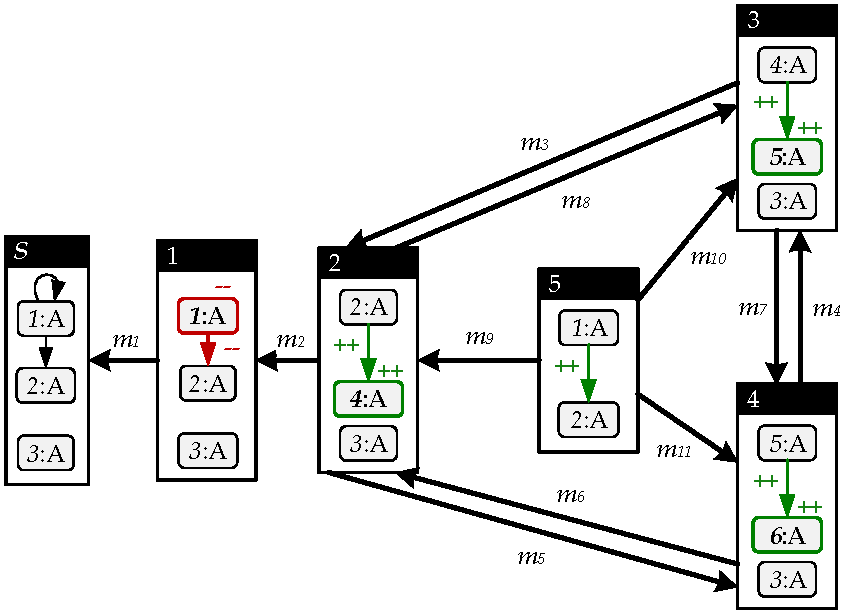
\includegraphics[width=.7\textwidth]{img/software_trans/graph_schema2.pdf}
\begin{math}
m_1=(1 \mapsto 1,2 \mapsto 2, 3 \mapsto 3);m_2=(2 \mapsto 2,3 \mapsto 3);m_3=(3 \mapsto 3, 4 \mapsto 4);m_4=(3 \mapsto 3, 5 \mapsto 5);m_5=(3 \mapsto 3, 2 \mapsto 6);m_6=(3 \mapsto 3,5 \mapsto 4);m_7=(3 \mapsto 3, 4 \mapsto 6);m_8=(2 \mapsto 5,3 \mapsto 3);m_9=(1 \mapsto 4,2 \mapsto 3);m_{10}=(1 \mapsto 5,2 \mapsto 3);m_{11}=(1 \mapsto 6,2 \mapsto 3)
\end{math}
\newline
\begin{math}
t_\GS(m_1)=S;s_\GS(m_1)=t_\GS(m_2)=\code{1};s_\GS(m_2)=s_\GS(m_5)=s_\GS(m_8)=t_\GS(m_3)=t_\GS(m_6)=t_\GS(m_9)=\code{2};s_\GS(m_3)=s_\GS(m_7)=t_\GS(m_4)=t_\GS(m_8)=t_\GS(m_{10})=\code{3};s_\GS(m_4)=s_\GS(m_6)=t_\GS(m_5)=t_\GS(m_7)=t_\GS(m_{11})=\code{4};s_\GS(m_9)=s_\GS(m_{10})=s_\GS(m_{11})=\code{5}
\end{math}
\end{center}
\caption{Recursive Graph Schema with Interweaving Cyclic Match-Paths}
\label{fig:sec-compl-software-trans:rec_graph_schema2}
\end{figure}

Finally, the semantics of a recursive graph schema is given by its graph language over the set of terminating recursive transformation sequences starting at start graph $S$.
Note that for some recursive graph schemata there may not exist a terminating recursive transformation sequence or a recursive transformation sequence at all and therefore, its language may be empty.
For example, the recursive graph schema in \cref{fig:sec-compl-software-trans:rec_graph_schema2} without rule \code{5} and adjacent matches $m_9$ to $m_{11}$ has no terminating match-path and therefore, no terminating recursive transformation sequence.
Moreover, for the complete schema in \cref{fig:sec-compl-software-trans:rec_graph_schema2} there exists an infinite set of terminating match-paths but all existing match-paths do not lead to a recursive transformation sequence due to violations of the gluing condition at the first match $m_1$ in each match-path.
The deletion of node \code{1:A} by applying rule \code{1} via match $m_1$ would result in a dangling reflexive edge on \code{1:A}.
Thus, in general, for a match-path there may not exists a corresponding recursive transformation sequence due to a violation of the gluing condition.

\begin{definition}[Graph Language of Recursive Graph Schemata]
\label{def:sec-compl-software-trans:lang_rec}
Let $\GS=((S,P),M,s_\GS,t_\GS)$ be a recursive graph schema.
The \emph{language $\Lang(\GS)$ of $\GS$}\index{recursive graph schema!language} is given by $\Lang(\GS):=\quotient{R(\GS)}{\sim}$ with $\quotient{R(\GS)}{\sim}$ being the quotient set of $R(\GS)$ by $\sim$, $R(\GS):=\{\der(t) \mid t\colon S \Trans{*}_\GS G, t \text{ is terminating}, t \text{ starts in }S\}$ being the set of all derived spans that are derivable by terminating recursive transformation sequences starting at start graph $S$ and $\sim$ being the equivalence relation on $R(\GS)$ where $g\colon S \to G \sim g'\colon S \to G'$ if and only if $G \cong G'$ with isomorphism $i\colon G \to G'$ and $i \circ g = g'$.
\envEndMarker
\end{definition}

\begin{remark}[Graph Language of Recursive Graph Schemata]
Note that $\sim$ is indeed an equivalence relation, i.e., 
\begin{enumerate*}
\item reflexivity: $g \sim g$ by isomorphism $i=\id_G\colon G \to G$ with $\id_G \circ g = g$,
\item symmetry: $g \sim g'$ if and only if $g' \sim g$ by inverse isomorphism $i^{-1}\colon G' \to G$ with $g=\id_G \circ g=i^{-1} \circ i \circ g\stackrel{\cref{def:sec-compl-software-trans:lang_rec}}{=} i^{-1} \circ g'$, and
\item transitivity: $g \sim g'$ and $g' \sim g''\colon S \to G''$ implies $g \sim g''$ by isomorphism $i' \circ i\colon G \to G''$ with isomorphism $i'\colon G' \to G''$ and $i' \circ i \circ g \stackrel{\cref{def:sec-compl-software-trans:lang_rec}}{=} i' \circ g' \stackrel{\cref{def:sec-compl-software-trans:lang_rec}}{=} g''$.
\end{enumerate*}
Moreover in $\M$-adhesive categories, $\paths=\paths'$ for $g=\der(t),g'=\der(t') \in R(\GS)$ with $t\colon S \Trans{path}_\GS G,t'\colon S \Trans{path'}_\GS G'$ implies $G \cong G'$ with isomorphism $i\colon G \to G'$ and $i \circ g = g'$ (thus, $g \sim g'$) by the uniqueness of pushout complements and pushout objects.
Furthermore, language $\Lang(\GS)$ may contain the same graph $G$ several times but each with different derived spans $\der(t_i)\colon S \to G$.
  \begin{center}
  \begin{tikzpicture}
  \node[inner sep=0pt] (a) at (0,0) {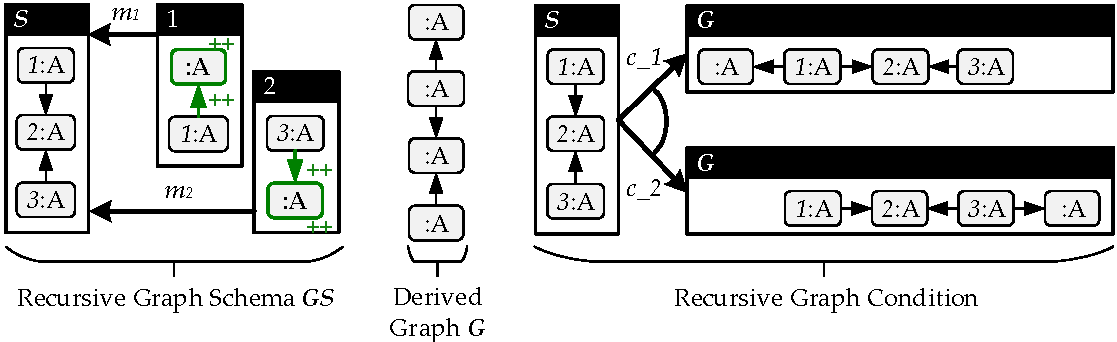
\includegraphics[width=.87\textwidth]{img/software_trans/graph_schema3.pdf}};
  \node[inner sep=0pt] (b) at (1.02,.55) {$\vee$};
  \end{tikzpicture}
  \end{center}
This is important in order to obtain recursive graph constraints over that language with the desired semantics.
For example, from the recursive graph schema $\GS$ from above, graph $G$ can be derived by two terminating recursive transformation sequences $t_1\colon S \Trans{(m_1)}_\GS G$ and $t_2\colon S \Trans{(m_2)}_\GS G$ starting at $S$, i.e., via the two match-paths $(m_1)$ and $(m_2)$, respectively.
The mappings along morphisms $m_1,m_2,c_1=\der(t_1)$ and $c_2=\der(t_2)$ are expressed by identifications of the numbers for each node.
Thus, $\Lang(\GS)=\{[c_1],[c_2]\}$ is given by two equivalence classes which contain one of the two derived spans to graph $G$, respectively, resulting in a recursive graph constraint $(\exists(S \trans{c_1} G,\true)) \vee (\exists(S \trans{c_2} G,\true))$ which disjoints both path-options.
Therefore, a graph $G'$ generally satisfies the constraint, if for all occurrences of pattern $S$ in $G'$
\begin{enumerate*}
\item[a)] either node \code{:A} is attached to the top node \code{1:A}, or
\item[b)] to the bottom node \code{3:A}.
\end{enumerate*}
\envEndMarker
\end{remark}

\begin{remark}[Graph Language of Recursive Graph Schemata]
Note that the language of a recursive graph schema may be empty if no terminating recursive transformations do exist: 
\begin{enumerate*}
\item either due to a violation of the gluing condition (cf. \cref{fig:sec-compl-software-trans:rec_graph_schema2}), or
\item no terminating match-paths do exist, or
\item the set of productions $P$ is empty.
\end{enumerate*}
This is true since an empty set $P$ implies that the set of matches $M$ is also empty and furthermore, the language is defined over recursive transformation sequences w.r.t. match paths and empty match paths (empty recursive transformation sequences) are not defined explicitly (cf. \cref{rem:sec-compl_software-trans:rec_trafo}).
\envEndMarker
\end{remark}

\begin{example}[Graph Language of Recursive Graph Schemata]
\label{ex:sec-compl-software-trans:lang_rec_schema}
For the recursive graph schema in \cref{ex:sec-compl-software-trans:rec_schema}, \cref{fig:sec-compl-software-trans:rec_graph_lang} illustrates all graphs that can be derived by terminating recursive transformation sequences with starting at start graph $S$.
This includes graph $G_0$ from below via recursive transformation $t_0\colon S \Trans{(m_1)}_\GS G_0$ and all graphs $G_1,G_2,G_3$ etc. that can be obtained from $G_0$ by arbitrarily adding a list of attribute (and class) nodes before $j$ (and after $i$) recursively via corresponding recursive transformations.
\begin{center}
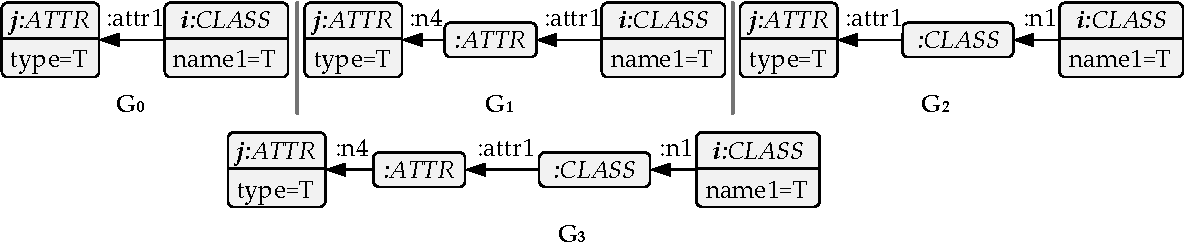
\includegraphics[width=.96\textwidth]{img/software_trans/graphs.pdf}
\end{center}
As the schema contains cyclic match-paths, its language is infinite containing equivalence class $[\der(t_0)\colon S \to G_0]$ and the infinite set of equivalence classes $[\der(t_i)\colon S \to G_i]$ of all other derived spans that can be obtained via terminating recursive transformations $t_i\colon S \Trans{*}_\GS G_i$ starting at $S$.
\envEndMarker
\end{example}

Based on the language of recursive graph schemata with start graph $S$ and productions $P$, we define recursive (infinite) graph conditions.
A recursive graph condition is defined by a disjunction over all derived spans of the language as mappings to the conclusion graphs with $S$ being the premise graph.
We assume a restriction of $P$ to productions that are non-deleting only in order to obtain an induced morphism as derived span for each pair of (premise,conclusion) graphs instead of spans of morphisms (cf. \cref{rem:sec-gc-gc:der_span_non_deleting}).

\begin{definition}[Recursive Graph Condition]
\label{def:sec-compl-software-trans:sem_rec_cond}
Let $\GS=((S,P),M,s_\GS,t_\GS)$ be a recursive graph schema with non-deleting productions $P$ and $\Lang(\GS)$ be the graph language of $\GS$.
The \emph{recursive graph condition $c_\GS$}\index{recursive graph condition} w.r.t. $\GS$ is defined by $c_\GS=\vee_{[\ac] \in \Lang(\GS)}\exists(\ac\colon S \to \_,\true)$.
\envEndMarker
\end{definition}

Recursive graph conditions are in $\M$-normal form which is necessary to be used in the verification of domain completeness in \cref{sec-dc-verification,thm:C-extensionCompleteness}.

\begin{proposition}[Recursive Graph Conditions in $\M$-normal form]
\label{prop:sec-compl-software-trans:rec_cond_constr_m_norm}
In $\M$-adhesive categories, \emph{each recursive graph condition is in $\M$-normal form}\index{recursive graph condition!$\M$-normal form}.
\envEndMarker
\end{proposition}

\begin{proof}
Technically, non-deleting productions $p=(L_p \transB{l_p} K_p \trans{r_p} R_p)$ are defined with $l_p=\id_{L_p}$ resulting in recursive transformation steps in \cref{def:sec-compl-software-trans:rec_trafo} with $l'_p \in \M$, $l'_p$ being an isomorphism, $l'^{-1}_p \in \M$ and $l'^{-1}_p$ being its inverse morphism for $\M$-adhesive categories.
This holds, since, the class $\M$ is closed under isomorphisms (therefore, $l_p \in \M$), iso- and $\M$-morphisms are closed under pushouts (therefore, $l'_p \in \M$ and $l'_p$ is isomorphism) and the inverse morphism $l'^{-1}_p$ is in $\M$ by $\M$-decomposition of $l'_p \circ l'^{-1}_p=\id_O \in \M$.
Furthermore, $r'_p \in \M$, since, $r_p \in \M$ by the definition of productions and $\M$-morphisms are closed under pushouts.
Thus, the induced morphisms $\ac$ in \cref{def:sec-compl-software-trans:sem_rec_cond} are in $\M$ by $\M$-composition of $r'_p \circ l'^{-1}_p$, i.e., recursive graph conditions are in $\M$-normal form.
\end{proof}

Note that recursive graph conditions are standard nested conditions and therefore, the standard logical operations for forming bigger conditions can be applied, e.g., negation, con- and dis-junction with other conditions.
Especially the possibility to negate recursive conditions not only allows the definition of graph constraints of the form ``For all $S$ there exists some regular path" and ``there exists $S$ with some regular path" but also ``For all $S$ there does not exist some regular path'' and ``there exists $S$ without some regular path''.

\begin{remark}[Conjunctive Recursive Graph Conditions]
Note that recursive graph conditions are explicitly defined by a disjunction over the conclusions that is infinite for infinite sets of conclusions.
A corresponding notion where the disjunction is replaced by a conjunction would disagree with the intrinsic idea of having an option of (infinite) conclusions.
Moreover, a conjunction over an infinite set of recursively growing conclusions as constraint can only be satisfied by infinite graphs. 
\envEndMarker
\end{remark}

\begin{example}[Recursive Graph Constraint]
\label{ex:sec-compl-software-trans:rec_cond}
For the recursive graph schema in \cref{ex:sec-compl-software-trans:rec_schema}, the corresponding infinite recursive graph constraint is generally satisfied by a graph $G$, if in $G$ for all attributes $A$ of type $T$ there is a class $C_1$ with name $T$ defined, and $A$ is the attribute of some class $C_2$ and either $C_1=C_2$ or $C_1$ is defined before $C_2$.
The membership of an attribute to a class is expressed by paths of \code{:attr1} and \code{:n4} edges between both.
The fact that a class is defined before some other class is expressed by paths of \code{:n1} edges between both.
\envEndMarker
\end{example}

In \cite{DBLP:conf/rta/BertrandDKSS12}, the decidability of reachability and coverability in various types of graph transformation systems with different restrictions were investigated.
In the following, we investigate the decidability of partial reachability in graph grammars and recursive graph schemata in order to conclude over the decidability of the satisfaction of recursive graph conditions in \cref{thm:sec-compl-software-trans:sat_rec_cond}.
In contrast to reachability, given a graph $G$, partial reachability of $G$ requires that there is at least one transformation sequence to some $G'$ such that there is an $\M$-morphism from $G'$ to $G$ instead of an isomorphism between both.
Conversely, coverability requires that there is at least one transformation sequence to some $G'$ such that there is an $\M$-morphism from $G$ to $G'$.
Thus, partial reachability is the inverse of coverability w.r.t. reachability.

While for finite-state graph transformation systems, the partial reachability problem is obviously decidable by iterating over all states and check partial reachability for each, it is different for infinite-state graph transformation systems (states are graphs and transitions between states are transformation steps).
We use infinite-state graph transformation systems for specifying infinite graph languages of recursive graph patterns.
While graph grammars with deleting rules can be used for specifying such languages where the start graph is the base case of the recursion and further graph patterns are obtained by recursively deleting and adding elements, the partial reachability problem is undecidable for general graph grammars by a reduction from the halting problem over turing machines (cf. \cref{prop:sec-compl-software-trans:dec_part_reach,item:sec-compl-software-trans:dec_part_reach2}).
However, for recursive graph schemata (with deleting rules), it turns out to be decidable by their monotone nature which is given by the restrictions for matches, since,
\begin{enumerate*}
\item matches are pre-defined, and
\item each recursive transformation step in a recursive transformation uses the co-match of the previous step to further restrict the match
\end{enumerate*} (cf. \cref{prop:sec-compl-software-trans:dec_part_reach,item:sec-compl-software-trans:dec_part_reach3}).
This leads to the decidability of the satisfaction of recursive graph conditions in \cref{thm:sec-compl-software-trans:sat_rec_cond}.

\begin{definition}[Partial Reachability Problem]
Let $G$ be a graph, $\GG=(S,P)$ be a graph grammar with start graph $S$ and a set of productions $P$ and $\GS=(\GG,M,s_\GS,t_\GS)$ be a recursive graph schema.
The \emph{partial reachability problem}\index{partial reachability!problem} for graph grammars (recursive graph schemata) is defined as follow: Is there a (terminating recursive) transformation sequence $S \Trans{*} G'$ ($S \Trans{*}_\GS G'$) that starts in $S$ to some graph $G'$ via productions $P$ (in $\GS$) such that there exists an $\M$-morphism $m\colon G' \to G,m \in \M$?
\envEndMarker
\end{definition}

% \begin{definition}[Monotone Graph Grammar]
% Let $<$ be a strict partial order over the set of graphs where $G < G'$ if and only if graph $G$ has fewer structural graph elements than $G'$.
% \emph{A graph grammar $\GG=(P,S)$ with productions $P$ and start graph $S$ is monotone} if for each transformation step $G \Trans{p \in P} G'$ with existing sequence $S \Trans{*} G$ via $P$ it holds that $G < G'$.
% \envEndMarker
% \end{definition}
% 
% Obviously, each typed attributed graph grammar $\GG=(P,S)$ with productions $P$ of the form $p\colon L \transB{l} K \trans{r} R,l,r \in \M$ and transformation steps based on the double pushout approach is monotone if $L < R$ for each production $p \in P$.
% In the following, we consider typed attributed graph grammars with non-deleting productions $p\colon L \to R \in \M$ only ($K=L$) and furthermore, $L < R$.
% Thus, each production of the grammar is non-trivial in the sense that it creates at least one graph element.

\begin{proposition}[Decidability of Partial Reachability]
\label{prop:sec-compl-software-trans:dec_part_reach}
\index{partial reachability!decidability}Let $G$ be a graph, $\GG=(S,P)$ be a graph grammar with start graph $S$ and a set of productions $P$ and $\GS=(\GG,M,s_\GS,t_\GS)$ be a recursive graph schema.
\begin{enumerate}
  \item For grammars $\GG$ with non-deleting productions $P$ only and finite graphs $G$, the (partial) reachability problem is decidable in $\M$-adhesive categories. 
  \item \label{item:sec-compl-software-trans:dec_part_reach2}In general and in particular for grammars $\GG$ with finite sets of productions $P$ and finite graphs $G$ in the $\M$-adhesive category $(\cat{Graphs}_\TG,\M)$ of typed graphs with(out) application conditions (and $\M$-matches), the (partial) reachability problem is undecidable.
  \item \label{item:sec-compl-software-trans:dec_part_reach3}In $(\cat{\AGraphs_\ATGI},\M)$, for recursive graph schemata $\GS$ with a finite set of matches $M$ and finite graphs $G$, the (partial) reachability problem is decidable.\envEndMarker
\end{enumerate}
\end{proposition}

\begin{proof}
The proof is presented in \cref{sec-proofs:prop:sec-compl-software-trans:dec_part_reach}.
\end{proof}

\begin{theorem}[Decidability of Satisfaction of Recursive Graph Conditions]
\label{thm:sec-compl-software-trans:sat_rec_cond}
\index{recursive graph condition!satisfaction!decidability}Let $\GS=((S,P),M,s_\GS,t_\GS)$ be a recursive graph schema with a finite set of matches $M$, $p\colon S \to G$ be a morphism ($G$ be a finite graph) and $c_\GS$ be the recursive graph condition w.r.t. $\GS$.
Then, \emph{the problem whether $p$ ($G$) satisfies $c_\GS$ is decidable in $\cat(\AGraphs_\ATGI,\M)$}.
\envEndMarker
\end{theorem}

\begin{proof}
By \cref{def:condition-satisfaction,def:sec-compl-software-trans:sem_rec_cond}, $p \models c_\GS=\vee_{[\der(t)] \in \Lang(\GS)}\exists(\der(t)\colon S \to \_,\true)$ if and only if $\exists [\der(t)\colon S \to G'] \in \Lang(\GS).p \models \exists(\der(t),\true) \Leftrightarrow \exists$ terminating recursive transformation $t$ in $\GS$ that starts in $S$ with $\der(t)\colon S \to G'$ and $p \models \exists(\der(t),\true) \Leftrightarrow\exists$ terminating recursive transformation $t\colon S \Trans{*}_\GS G'$ in $\GS$ that starts in $S$ such that there exists $q\colon G' \to G \in \M$ with $q \circ \der(t)=p$ which is decidable by \cref{prop:sec-compl-software-trans:dec_part_reach,item:sec-compl-software-trans:dec_part_reach3} by checking the commuting property for all existing $q \in \M$ which also terminates with the procedure from the proof of \cref{prop:sec-compl-software-trans:dec_part_reach,item:sec-compl-software-trans:dec_part_reach3} for finite $G$.
For recursive graph constraints $c_\GS$ over $S$, listing all occurrences of $S$ in $G$ (all $p\colon S \to G \in \M$) also terminates and results in a finite set for finite $G$.
For each occurrence of $S$ in $G$ we can proceed with $c_\GS$ as given above.
\end{proof}

Recursive structures in recursive conditions are expressed by cycles of matches $M$ in the underlying recursive graph schema.
Thus, a recursive graph schema with cycles in $M$ may lead to an infinite recursive graph constraint which is constructed step-wise by pumping the underlying condition via the repeated iteration of cycles.
The verification procedure of domain completeness terminates for finite graph constraints only.
Therefore, we present two techniques for deriving finite constraints from infinite recursive graph constraints by making them tighter or weaker.
The idea behind tightened recursive graph conditions is to omit all conclusion graphs from an infinite recursive condition $c_\GS$ that exceed a specific upper bound.
The upper bound is defined by a dedicated graph $G_u$ and the tightened condition of $c_\GS$ is formed over all conclusion graphs of $c_\GS$ with inclusions to $G_u$ only.
Therefore, the set of graphs satisfying a set of tightened constraints is a subset of the set of graphs satisfying the set of the corresponding originial infinite constraints but not necessarily vice versa.
However, it holds that a successful verification of domain completeness w.r.t. the tightened constraints and a given TGG implies that all graphs up to the upper bound satisfying the original infinite constraints can be completely transformed via the TGG.
In contrast to that, the idea behind weakened recursive graph conditions is to list for each acyclic, terminating recursive transformation sequence $S \Trans{\paths}_\GS G$ over $\GS$ and for all match-cycles in $\GS$ that are reachable from match-path $\paths$ all relevant overlappings of a single iteration of each cycle and $G$ as conclusion graphs.
Therefore, the derived conditions cover those graph structures only that may occur when iterating each cycle the last time by omitting those structures that are created by the iterations in between.
For positive recursive constraints $c_\GS$, the set of graphs satisfying the corresponding weakened constraint is a superset of the set of graphs satisfying $c_\GS$.
Thus, a successful verification of domain completeness w.r.t. weakened constraints and a given TGG implies domain completeness w.r.t. the original (infinite) constraints $c_\GS$ and TGG which implies furthermore that all graphs satisfying constraints $c_\GS$ can be completely transformed via the TGG.

\begin{definition}[Tightened Graph Language of Recursive Graph Schemata]
\label{def:sec-dc-general-rec:t_g_lang}
Let $\GS=((S,P),M,s_\GS,t_\GS)$ be a recursive graph schema.
Let $\Lang(\GS)$ be the graph language of $\GS$ and graph $G_u$ be an upper bound.
The \emph{tightened language $\Lang_t(\GS,G_u) \subseteq \Lang(\GS)$}\index{recursive graph schema!language!tightened} of $\GS$ and w.r.t. $G_u$ is given by $\Lang_t(\GS,G_u):=\{[\ac] \mid [\ac\colon S \to G] \in \Lang(\GS),\exists i\colon G \to G_u \in \M\}$.
\envEndMarker
\end{definition}

Before defining weakened conditions, we define the notions of $\M$-decomposition, initial $\M$-subobject and weakened language of recursive graph schemata at first.
An $\M$-decomposition of a morphism $\tr\colon A \to B$ is a decomposition of $\tr$ into two morphisms $\tr_1\colon A \to C,\tr_2\colon C\to B$ where both $\tr_1$ and $\tr_2$ are in $\M$.
For example in $(\cat{\Graphs},\M)$, $\M$-decompositions are a restriction of general decompositions of morphisms in the sense that graph $A$ is guaranteed to be a sub-graph of $C$ and $C$ is a sub-graph of $B$ whereas in general decompositions $C$ may be ``bigger'' than $B$ with an non-injective morphism $\tr_2$.
Similar to the concept of an $\M$-initial object which is considered as the ``smallest'' $\M$-subobject of all objects of a category, we introduce the weaker notion of an initial $\M$-subobject which is only the ``smallest" $\M$-subobject concerning one object of a category, respectively.
While a category may not have an $\M$-initial object, it may have an initial $\M$-subobject for each object.
 
\begin{definition}[$\M$-decomposition of Morphisms]
\emph{An $\M$-decomposition $d$ of an $\M$-morphism $\tr\colon L \to R$}\index{$\M$-decomposition of morphisms}, in short $\tr$-$\M$-decomposition, consists of two $\M$-morphisms $d=(L \trans{\tr_1} L' \trans{\tr_2} R)$ with $\tr_2 \circ \tr_1 = \tr$ and $\tr_1, \tr_2 \in \M$.
\envEndMarker
\end{definition}

\begin{definition}[Initial $\M$-subobject]
\label{def:sec-compl-software-trans:in_M_subobj}
Given an $\M$-adhesive category $(\cat{C},\M)$ and an object $G \in \cat{C}$.
Then, \emph{$\M$-subobject $[i_G\colon I_G \to G \in \M]$ of $G$ is initial}\index{$\M$-subobject!initial}, if for each $\M$-subobject $[a\colon A \to G \in \M]$ of $G$ there exists an (unique) $\M$-morphism $i_A\colon I_G \to A \in \M$ with $a \circ i_A = i_G$.
An $\M$-adhesive category $(\cat{C},\M)$ has initial $\M$-subobjects, if for each object $G \in \cat{C}$ there exists an initial $\M$-subobject.
\envEndMarker
\end{definition}

\begin{remark}[Initial $\M$-subobject]
\label{rem:sec-compl-software-trans:in_M_subobj}
Note that the uniqueness of morphism $i_A$ is optional as it follows directly from $a \in \M$ with $\M$ being a class of monomorphisms, since, $i_{A,1},i_{A,2} \in \M$ with $a \circ i_{A,1}=i_G=a \circ i_{A,2}$ implies that $i_{A,1}=i_{A,2}$.
\envEndMarker
\end{remark}

Initial $\M$-subobjects can be constructed by the extremal $\E$-$\M$-factorisation of initial morphisms.
Furthermore, initial $\M$-subobjects are unique up to isomorphism.

\begin{proposition}[Construction \& Uniqueness of Initial $\M$-subobjects]
\label{prop:sec-compl-software-trans:constr_uniqu_init_msubobj}
Given an $\M$-adhesive category $(\cat{C},\M)$ with an extremal $\E$-$\M$-factorisation and initial object $I$.
Then, \emph{the initial $\M$-subobject $[i_{G,2}\colon I_G \to G \in \M]$ for an object $G \in \cat{C}$ can be constructed}\index{$\M$-subobject!initial!construction} by the extremal $\E$-$\M$-factorisation $i_{G,2} \circ i_{G,1}=i_G$ of the initial morphism $i_G\colon I \to G$ with $i_{G,1}\colon I \to I_G \in \E,i_{G,2}\colon I_G \to G \in \M$.
Furthermore, in $\M$-adhesive categories, \emph{initial $\M$-subobjects are unique up to isomorphism}\index{$\M$-subobject!initial!uniqueness}.
\envEndMarker
\end{proposition}

\begin{proof}
We have to show that $\M$-subobject $[i_{G,2}\colon I_G \to G \in \M]$ of $G$ is initial.
\begin{center}
\begin{tikzpicture}[]
\fill (0,0) node[inner sep=1pt] (I) {$I$};
\fill (0,0) node[below of=I,yshift=-.5cm,inner sep=1pt] (IG) {$I_G$};
\fill (0,0) node[below of=IG,yshift=-.5cm,inner sep=1pt] (G) {$G$};
\fill (0,0) node[left of=IG,xshift=-2.5cm,inner sep=1pt] (A) {$A$};
\fill (0,0) node[right of=A,xshift=.75cm,yshift=.3cm,inner sep=1pt] (O) {$O$};
\fill (0,0) node[right of=IG,xshift=-.25cm,inner sep=1pt] (1) {$(=)$};
\fill (0,0) node[right of=O,xshift=.2cm,yshift=.3cm,inner sep=1pt] (2) {$(=)$};
\fill (0,0) node[left of=O,xshift=.5cm,yshift=.45cm,inner sep=1pt] (3) {$(=)$};
\fill (0,0) node[below of=O,inner sep=1pt] (4) {$(1)$};
%
\fill (0,0) node[right of=G,xshift=5cm,inner sep=1pt] (G2) {$\overline{G}$};
\fill (0,0) node[right of=IG,xshift=3cm,inner sep=1pt] (IG1) {$\overline{I}_{G,1}$};
\fill (0,0) node[right of=IG,xshift=7cm,inner sep=1pt] (IG2) {$\overline{I}_{G,2}$};
\fill (0,0) node[right of=I,xshift=5cm,inner sep=1pt] (O2) {$\overline{O}$};
\fill (0,0) node[above of=G2,yshift=.25cm,inner sep=1pt] (5) {$(2)$};
%
{
\pgfsetarrows{right hook-latex}
\path (A) edge[bend right=30] node[fill=white]{\scriptsize{$a$}} (G);
\path (O) edge[] node[above]{\scriptsize{$o_2$}} (IG);
\path (IG1) edge[] node[fill=white]{\scriptsize{$\overline{i}_{G,1}$}} (G2);
\path (O2) edge[] node[fill=white]{\scriptsize{$o_2$}} (IG2);
\path (IG1) edge[dotted,bend right=35] node[fill=white]{\scriptsize{$o'_1$}} (O2);
%
\pgfsetarrows{left hook-latex}
\path (O) edge[] node[above]{\scriptsize{$o_1$}} (A);
\path (IG) edge[] node[right]{\scriptsize{$i_{G,2}$}} (G);
\path (IG) edge[bend left=35,dotted] node[below]{\scriptsize{$o_2^{-1}$}} (O);
\path (IG2) edge[] node[fill=white]{\scriptsize{$\overline{i}_{G,2}$}} (G2);
\path (O2) edge[] node[fill=white]{\scriptsize{$o_1$}} (IG1);
\path (IG2) edge[dotted,bend left=35] node[fill=white]{\scriptsize{$o'_2$}} (O2);
%
\pgfsetarrows{-latex}
\path (I) edge[in=0,out=0,looseness=1.5] node[fill=white]{\scriptsize{$i_G$}} (G);
\path (I) edge[in=90,out=180] node[fill=white]{\scriptsize{$i_A$}} (A);
\path (I) edge[dotted] node[fill=white]{\scriptsize{$i_O$}} (O);
%
\pgfsetarrows{->>}
\path (I) edge[] node[right]{\scriptsize{$i_{G,1}$}} (IG);
}
\end{tikzpicture}
\end{center}
Let $[a\colon A \to G \in \M]$ be an $\M$-subobject of $G$ and $i_A\colon I \to A$ be the initial morphism to $A$.
We construct pullback $(1)$ $(o_1,o_2)$ over morphisms $(a,i_{G,2})$.
By $\M$-morphisms are closed under pullbacks, $o_1,o_2 \in \M$.
By the uniqueness of the initial morphism, $i_G=i_{G,2} \circ i_{G,1}=a \circ i_A$.
Thus, by the universal property of pullbacks, there exists a unique morphism $i_O\colon I \to O$ with $o_1 \circ i_O=i_A$ and $o_2 \circ i_O=i_{G,1}$.
By the definition of class $\E$ with $i_{G,1} \in \E$ and $o_2 \in \M$, $o_2$ is an isomorphism with inverse isomorphism $o_2^{-1} \in \M$ and $o_2 \circ o_2^{-1} = \id_{I_G}$ $^{(*^1)}$, since, class $\M$ is closed under isomorphisms.
By $\M$-composition, $o_1 \circ o_2^{-1} \in \M$, $o_1 \circ o_2^{-1}$ is unique by \cref{rem:sec-compl-software-trans:in_M_subobj} and furthermore, $a \circ o_1 \circ o_2^{-1} \stackrel{(1)}{=} i_{G,2} \circ o_2 \circ o_2^{-1} \stackrel{(*^1)}{=} i_{G,2} \circ \id_{I_G} = i_{G,2}$.
The resulting initial $\M$-subobjects of the presented construction are unique, since, extremal $\E$-$\M$-factorisations are unique up to isomorphism in the given $\M$-adhesive category.
In general, apart from the construction, the uniqueness of initial $\M$-subobjects in $\M$-adhesive categories is shown as follows.
Given two initial $\M$-subobjects $[\overline{i}_{G,1}\colon \overline{I}_{G,1} \to \overline{G} \in \M]$ and $[\overline{i}_{G,2}\colon \overline{I}_{G,2} \to \overline{G} \in \M]$ of $\overline{G}$.
We construct pullback $(2)$ $(o_1,o_2)$ over $(\overline{i}_{G,1},\overline{i}_{G,2})$ with $o_1,o_2 \in \M$, since, $\M$-morphisms are closed under pullbacks and furthermore, $\overline{i}_{G,1} \circ o_1,\overline{i}_{G,2} \circ o_2\in \M$ by $\M$-composition.
By \cref{def:sec-compl-software-trans:in_M_subobj}, there exists $o'_2\colon \overline{I}_{G,2} \to \overline{O} \in \M$ with $\overline{i}_{G,1} \circ o_1 \circ o'_2=\overline{i}_{G,2}$ $^{(*^1)}$.
Analogously, there exists $o'_1\colon \overline{I}_{G,1} \to \overline{O} \in \M$ with $\overline{i}_{G,1} \circ \id_{\overline{I}_{G,1}} = \overline{i}_{G,1} = \overline{i}_{G,2} \circ o_2 \circ o'_1 \stackrel{(*^1)}{=} \overline{i}_{G,1} \circ o_1 \circ o'_2 \circ o_2 \circ o'_1$.
By $\overline{i}_{G,1} \in \M$ and $\M$ being a class of monomorphisms, $o_1 \circ o'_2 \circ o_2 \circ o'_1=\id_{\overline{I}_{G,1}}$.
Conversely, $\overline{i}_{G,2} \circ \id_{\overline{I}_{G,2}} = \overline{i}_{G,2} \stackrel{(*^1)}{=} \overline{i}_{G,1} \circ o_1 \circ o'_2 = \overline{i}_{G,2} \circ o_2 \circ o'_1 \circ o_1 \circ o'_2$.
By $\overline{i}_{G,2} \in \M$ being a monomorphism, $o_2 \circ o'_1 \circ o_1 \circ o'_2 = \id_{\overline{I}_{G,2}}$.
Thus, $o_2 \circ o'_1$ is an isomorphism with commuting $(2)$.
\end{proof}

\begin{example}[Initial $\M$-subobject]
The category $(\cat{\AGraphs_\ATGI},\M)$ has $(\varnothing,T_\DSIG)$ as initial object with $\varnothing$ being the empty graph except for the data nodes and $T_\DSIG$ being the term algebra of data signature $\DSIG$.
The initial $\M$-subobject of an object $(G,D) \in \cat{\AGraphs_\ATGI}$ is constructed by the extremal $\E$-$\M$-factorisation of the initial morphism $i_G\colon (\varnothing,T_\DSIG) \to (G,D)$.
Thus, the initial $\M$-subobject of $(G,D)$ with $\DSIG$-algebra $D$ is $[i'_G\colon (\varnothing,D) \to (G,D) \in \M]$ with $\varnothing$ being the empty graph except for the data nodes and $i'_G=(i'_{G,G},i'_{G,D})$ being the empty morphism $i'_{G,G}\colon \varnothing \to G$ on the graph part and identity $i'_{G,D}=\id_D\colon D \to D$ on the data part.
Note that, $(\cat{\AGraphs_\ATGI},\M)$ has an initial object but no $\M$-initial object, since, $\M$-morphisms are isomorphisms on the data part and this does not hold for all initial morphisms in $(\cat{\AGraphs_\ATGI},\M)$.
\envEndMarker
\end{example}

The result in \cref{prop:sec-compl-software-trans:init_M_subobj_along_M} we use to prove the well-definedness of the construction of weakened languages of recursive graph schemata in \cref{prop:sec-compl-software-trans:weakened_lang_well_def}.

\begin{proposition}[Initial $\M$-subobjects along $\M$-Morphisms]
\label{prop:sec-compl-software-trans:init_M_subobj_along_M}
In an $\M$-adhesive category with initial $\M$-subobjects, let $a\colon A \to B \in \M$ be an $\M$-morphism and $[i_A\colon I_A \to A \in \M]$ be the initial $\M$-subobject of $A$.
Then, \emph{$[a \circ i_A\colon I_A \to B]$ is the initial $\M$-subobject of $B$}\index{$\M$-subobject!initial!along $\M$}.
\envEndMarker
\end{proposition}

\begin{proof}
By $\M$-composition $a \circ i_A \in \M$, i.e., $[a \circ i_A \in \M]$ is an $\M$-subobject of $B$.
Let $[i_B\colon I_B \to B \in \M]$ be the initial $\M$-subobject of $B$.
Then, there exists an unique morphism $i_{I_A}\colon I_B \to I_A \in \M$ with $a \circ i_A \circ i_{I_A}=i_B$ $^{(*^1)}$.
By $\M$-composition, $[i_A \circ i_{I_A} \in \M]$ is an $\M$-subobject of $A$.
Thus from $i_A$ being the initial $\M$-subobject of $A$ by assumption, there is $i_{I_B}\colon I_A \to I_B \in \M$ with $i_A \circ i_{I_A} \circ i_{I_B}=i_A=i_A \circ \id_{I_A} \stackrel{i_A\text{ is Mono}}{\Rightarrow} i_{I_A} \circ i_{I_B}=\id_{I_A}$ $^{(*^2)}$.
Moreover, $i_B \circ i_{I_B}\stackrel{(*^1)}{=}a \circ i_A \circ i_{I_A} \circ i_{I_B} \stackrel{(*^2)}{=} a \circ i_A$ $\Rightarrow i_B \circ i_{I_B} \circ i_{I_A}=a \circ i_A \circ i_{I_A} \stackrel{(*^1)}{=} i_B=i_B \circ \id_{I_B}$ $\stackrel{i_B\text{ is Mono}}{\Rightarrow} i_{I_B} \circ i_{I_A}=\id_{I_B}$ $^{(*^3)}$.
\begin{center}
\begin{tikzpicture}[]
\fill (0,0) node[inner sep=1pt] (IB) {$I_B$};
\fill (0,0) node[below of=IB,yshift=-.5cm,inner sep=1pt] (IA) {$I_A$};
\fill (0,0) node[right of=IA,xshift=1cm,inner sep=1pt] (A) {$A$};
\fill (0,0) node[right of=A,xshift=1cm,inner sep=1pt] (B) {$B$};
%
\fill (0,0) node[right of=IA,xshift=.5cm,yshift=.5cm,inner sep=1pt] (1) {$(1)$};
%
{
\pgfsetarrows{right hook-latex}
\path (IB) edge[] node[fill=white]{\scriptsize{$i_B$}} (B);
\path (IA) edge[] node[fill=white]{\scriptsize{$i_A$}} (A);
\path (A) edge[] node[fill=white]{\scriptsize{$a$}} (B);
\path (IB) edge[dotted, bend left=45] node[fill=white]{\scriptsize{$i_{I_A}$}} (IA);
\path (IA) edge[dotted, bend left=45] node[fill=white]{\scriptsize{$i_{I_B}$}} (IB);
%
\pgfsetarrows{left hook-latex}
%
\pgfsetarrows{-latex}
%
\pgfsetarrows{->>}
%
}
\end{tikzpicture}
\end{center}
By $(*^1),(*^2)$ and $(*^3)$, $i_{I_A}$ is an isomorphism with $(1)$ commutes and therefore, $[i_B]=[a \circ i_A]$.
\end{proof}

For the construction of weakened graph languages, we restrict productions to be non-deleting in order to avoid conflicts with violations of the gluing condition and introduce the equivalence of match-cycles (cf. \cref{rem:sec-compl-software-trans:con_weakened_lang}).
We are confident that the construction can be extended to general productions by integrating gluing condition checks.

\begin{definition}[Equivalence of Match-Cycles]
\label{def:sec-dc-general-rec:equ_match_cycles}
Let $\gg((m_i)_{i \in \{1\ldots n\}}):=\{(m_i,m_{i+1}) \mid 1 \leq i < n\} \cup \{(m_n,m_1)\}$ be an order over the matches of a given match-cycle $(m_i)_{i \in \{1\ldots n\}}$.
\emph{Two match-cycles $\paths_1$ and $\paths_2$ are equal up to shifting of matches}\index{match-path!match-cycle!equivalence up to shifting of matches} if and only if $\gg(\paths_1)=\gg(\paths_2)$.
Let $\GS$ be a recursive graph schema and $\paths$ be a match-cycle in $\GS$.
With $\gg_\GS(\paths):=\{\paths' \mid \text{$\paths'$ is match-cycle in $\GS$},\gg(\paths)=\gg(\paths')\}$ we denote the set of all match-cycles in $\GS$ that are equal to $\paths$ up to shifting of matches.
For match-paths $\paths$ in $\GS$ that are no match-cycles, we define $\gg_\GS(\paths):= \varnothing$.
Let $\Paths_{\_,\_}(\GS)$ be the set of all acyclic match-cycles in $\GS$ and $\sim$ be the equivalence relation on $\Paths_{\_,\_}(\GS)$ where $\paths_1 \sim \paths_2$ if and only if $\gg_\GS(\paths_1)=\gg_\GS(\paths_2)$.
With $\quotient{\Paths_{\_,\_}(\GS)}{\sim}$ we denote the equivalence classes of all acyclic match-cycles in $\GS$ that are equal up to shifting of matches.
\envEndMarker
\end{definition}

\begin{example}[Equivalence of Match-Cycles]
For the match-cycle $\paths=(m_7,m_8,m_6)$ in \cref{fig:sec-compl-software-trans:rec_graph_schema2}, $\gg_\GS(\paths)=\{(m_7,m_8,m_6),(m_6,m_7,m_8),(m_8,m_6,m_7)\}$.
\envEndMarker
\end{example}

\begin{definition}[Weakened Graph Language of Recursive Graph Schemata]
\label{def:sec-compl-software-trans:weakened_lang}
Let $\GS=((S,P),M,s_\GS,t_\GS)$ be a recursive graph schema with non-deleting productions $P$.
The \emph{weakened language $\Lang_w(\GS):=\quotient{\underline{\Lang}_w(\GS)}{\sim}$ of $\GS$}\index{recursive graph schema!language!weakened} is given by the quotient set of $\underline{\Lang}_w(\GS)$ by $\sim$ with $\sim$ being the equivalence relation from \cref{def:sec-compl-software-trans:lang_rec} and projection $\underline{\Lang}_w(\GS):=\{\ac \mid (\ac,n) \in \cup_{m \in \underline{\Paths}_S(\GS)}(\underline{\Lang}_w(m,1,\id_S,\id_S,1))\}$ with $\underline{\Paths}_S(\GS) \subseteq \Paths_S(\GS)$ being the set of all acyclic and terminating match-paths in $\GS$ that start in $S$ with construction $\underline{\Lang}_w$ as given inductively below.
\envEndMarker
\end{definition}

\begin{paragraph}{Construction}
\begin{center}
	$\underline{\Lang}_w((m_i)_{i \in \{1\ldots j\}},i,\ac,n,k)=\begin{cases}
	\cup_{(t,n') \in \mathcal{B}}(\underline{\Lang}_w((m_i)_{i \in \{1\ldots j\}}, i+1, & \text{, for } \ac\colon \_ \to A \text{ and}\\
	\der(t)\circ \ac,n',1)) \text{ with } \mathcal{B}= & \text{if } i \leq j \text{ and }\\
	\{(t,n') \mid t\colon A \Trans{(s_\GS(m_i),m_i,n)}_{\GS,n'} B\} & (\Pset = \varnothing \text{ or } k=2)\\
	\cup_{(\ac',n') \in \mathcal{C}}(\underline{\Lang}_w((m_i)_{i \in \{1\ldots j\}},i, & \text{, for } \ac\colon \_ \to A \text{ and}\\
	\ac',n',2)) \text{ with } \mathcal{C}=\{(\ac,n)\} \cup & \text{if } i \leq j \text{ and }\\
	\cup_{\paths \in \Pset}(A \oplus B_\paths) \text{ where } & \Pset \neq \varnothing\\
	B_\paths=\underline{\Lang}_w(\paths,1,\id_R,\id_R,2) \text{ for} & \\
	\paths=(m'_k)_{k \in \{1\ldots l\}} \text{ and } m'_1\colon L \to R & \\
	\{(\ac,n)\} & \text{, otherwise}\\
	\end{cases}$
\end{center}
with switch $k \in \{1,2\}$, $\overline{\Pset}=\Paths_{t_\GS(m_i),t_\GS(m_i)}(\GS) \setminus \gg_\GS((m_i)_{i \in \{1\ldots j\}})$ being the set of all match-cycles in $\GS$ that start and end in $t_\GS(m_i)$ except all paths that are equal up to shifting to the path that is currently being handled, $\Pset \subseteq \overline{\Pset}$ being all paths in $\overline{\Pset}$ that are acyclic and $\oplus$ defined as follows:
$A \oplus B_\paths:=\cup_{d \in \mathcal{D}}(\{(a'_2 \circ \ac,a'_1 \circ \overline{n}') \mid \cond\})$ where in contrast to $(\ac,n) \in \mathcal{C}$ which represents the case with no iterations of cycles via match-path $\paths \in \Pset$, $A \oplus B_\paths$ represents arbitrary iterations by forming all relevant overlappings of the result of a single iteration $\iter \in B_\paths$ and $A$ where:
\begin{center}
\begin{tikzpicture}[]
\fill (0,0) node[inner sep=1pt] (I) {$I_L$};
\fill (0,0) node[right of=I,xshift=1cm,inner sep=1pt] (I') {$I'_{L}$};
\fill (0,0) node[right of=I',xshift=1cm,inner sep=1pt] (Lk') {$L$};
\fill (0,0) node[right of=Lk',xshift=4cm,inner sep=1pt] (Gk) {$L'$};
\fill (0,0) node[below of=Lk',yshift=-.5cm,inner sep=1pt] (R) {$R$};
\fill (0,0) node[below of=R,yshift=-.5cm,inner sep=1pt] (G2) {$R$};
\fill (0,0) node[below of=G2,yshift=0cm,inner sep=1pt] (G) {$A$};
\fill (0,0) node[right of=Lk',xshift=3cm,inner sep=1pt] (O) {$O$};
\fill (0,0) node[right of=G2,xshift=3cm,inner sep=1pt] (G'') {$R''$};
\fill (0,0) node[right of=G,xshift=4cm,inner sep=1pt] (G') {$A'$};
%
\fill (0,0) node[right of=R,xshift=.25cm,yshift=1cm,inner sep=1pt] (4) {$(2)$};
\fill (0,0) node[right of=R,xshift=2cm,yshift=0cm,inner sep=1pt] (5) {$(3)$};
\fill (0,0) node[right of=G2,xshift=.25cm,yshift=.5cm,inner sep=1pt] (6) {$(4)$};
\fill (0,0) node[right of=R,xshift=3.5cm,yshift=0cm,inner sep=1pt] (7) {$(5)$};
%
\fill (0,0) node[left of=I,xshift=-1cm,inner sep=1pt] (R3) {$R$};
\fill (0,0) node[below of=R3,xshift=-2cm,yshift=-.5cm,inner sep=1pt] (L2) {$L$};
\fill (0,0) node[right of=L2,xshift=1cm,inner sep=1pt] (L'2) {$L'$};
\fill (0,0) node[below of=L2,xshift=0cm,yshift=-.5cm,inner sep=1pt] (R2) {$R$};
\fill (0,0) node[right of=R2,xshift=1cm,inner sep=1pt] (R'2) {$R'$};
%
\fill (0,0) node[right of=L2,xshift=0cm,yshift=-.75cm,inner sep=1pt] (8) {$(PO)$};
\fill (0,0) node[right of=L'2,xshift=-.5cm,inner sep=1pt] (9) {$(=)$};
%
{
\pgfsetarrows{right hook-latex}
\path (I) edge[] node[fill=white]{\scriptsize{$i_{L,1}$}} (I');
\path (I') edge[] node[fill=white]{\scriptsize{$i_{L,2}$}} (Lk');
\path (Lk') edge[bend left=25] node[fill=white]{\scriptsize{$\overline{\ac}'$}} (Gk);
\path (I') edge[bend right=45] node[fill=white]{\scriptsize{$m$}} (R);
\path (Lk') edge[dotted] node[fill=white]{\scriptsize{$o$}} (O);
\path (R) edge[dotted] node[fill=white]{\scriptsize{$o'$}} (O);
\path (G2) edge[dotted] node[fill=white]{\scriptsize{$\der(t)$}} (G'');
\path (G) edge[bend right=25,dotted] node[fill=white]{\scriptsize{$a'_2$}} (G');
%
\path (R2) edge[] node[fill=white]{\scriptsize{$\overline{\ac}$}} (R'2);
\path (L2) edge[dotted] node[fill=white]{\scriptsize{$\overline{\ac}'$}} (L'2);
%
\pgfsetarrows{left hook-latex}
\path (Lk') edge[] node[fill=white]{\scriptsize{$m'_1$}} (R);
\path (R) edge[] node[fill=white]{\scriptsize{$\id_R$}} (G2);
\path (G2) edge[] node[left]{\scriptsize{$n$}} (G);
\path (O) edge[dotted] node[fill=white]{\scriptsize{$a''$}} (G'');
\path (R) edge[dotted] node[fill=white]{\scriptsize{$n'$}} (G'');
\path (Gk) edge[dotted] node[fill=white]{\scriptsize{$a'_1$}} (G');
%
\path (L2) edge[] node[fill=white]{\scriptsize{$m'_1$}} (R2);
\path (L'2) edge[dotted] node[fill=white]{\scriptsize{$\overline{m}'_1$}} (R'2);
\path (R3) edge[bend left=75] node[fill=white]{\scriptsize{$\overline{n}$}} (R'2);
\path (R3) edge[dotted] node[fill=white]{\scriptsize{$\overline{n}'$}} (L'2);
%
\pgfsetarrows{-latex}
%
\pgfsetarrows{->>}
%
}
\end{tikzpicture}
\end{center}
\begin{enumerate}
  \item \label{item:sec-compl-software-trans:weakened_lang:1}$\mathcal{D}=\{d=(I_L \trans{i_{L,1}} I'_L \trans{i_{L,2}} L) \mid d \text{ is } i_L \text{-} \M \text{-decomposition for initial } \M \text{-subobject } [i_L\colon I_L \to L \in \M] \text{ of } L\}$, and
  \item $\cond$:
  \begin{enumerate}
    \item \label{item:sec-compl-software-trans:weakened_lang:2a}$\iter=(\overline{\ac}\colon R \to R',\overline{n}\colon R \to R') \in B_\paths$,
	\item \label{item:sec-compl-software-trans:weakened_lang:2b}$(a'_1\colon L' \to A',a'_2\colon A \to A')$ is pushout over $(\overline{\ac}' \circ i_{L,2},n \circ m)$,
    \item \label{item:sec-compl-software-trans:weakened_lang:2c}$(\overline{\ac}' \in \M,\overline{m}'_1 \in \M)$ is pushout complement over $(m'_1,\overline{\ac})$ resulting in pushout $(PO)$ with induced morphism $\overline{n}' \in \M$ and $\overline{m}'_1 \circ \overline{n}'=\overline{n}$, 
    \item \label{item:sec-compl-software-trans:weakened_lang:2e}$m\colon I'_L \to R \in \M$ such that $\exists t\colon R \Trans{p'}_{\GS,n'} R''$ with $p' \in \overline{\Pset}$ or $\der(t)=n'=\id_R$ such that
    \begin{enumerate*}
    \item \label{item:sec-compl-software-trans:weakened_lang:2e1}$\exists a''\colon O \to R'' \in \M$ for pushout $(o,o')$ over $(i_{L,2},m)$ with
    \item \label{item:sec-compl-software-trans:weakened_lang:2e2}$(2)+(3)$ commutes, and
    \item \label{item:sec-compl-software-trans:weakened_lang:2e3}$(3)+(4)$ commutes.\envEndMarker
    \end{enumerate*}   
  \end{enumerate}
\end{enumerate}
\end{paragraph}

\begin{remark}[Construction of Weakened Graph Languages]
\label{rem:sec-compl-software-trans:con_weakened_lang}
The construction is based on the idea that cyclic, terminating match-paths are obtained from acyclic, terminating paths by possibly pumping the path after each match by adding arbitrary match-cycles.
Therefore, the construction starts with an acyclic, terminating match-path $m$ in $\GS$ that starts in $S$, $\id_S$ for $\ac$ as derived span, $\id_S$ for $n$ as co-match and switch $k=1$.
The construction passes through $m$ step-wise with matches $m_i \in m$:
\begin{enumerate}
  \item \label{item:sec-compl-software-trans:cons_weakened_lan:1} If there is no match-cycle from and to the target $t_\GS(m_i)$ of $m_i$ which differs from all paths that are equal to the path that is currently being handled up to shifting of matches ($\mathcal{P}=\varnothing$) and that may lead to a cyclic match-path before $m_i$ or if switch $k=2$, then a recursive transformation step $t$ with co-match $n'$ is performed via production $s_\GS(m_i)$, match $m_i$ and co-match $n$.
  The construction recursively proceeds with the next match in $m$ for $m_i$, an extended derived span $\der(t) \circ \ac$ for $\ac$, co-match $n'$ for $n$ and switch $k=1$.
  \item If there is a match-cycle from and to $t_\GS(m_i)$ which differs from all paths that are equal to the path that is currently being handled up to shifting of matches ($\mathcal{P}\neq\varnothing$), then before performing the recursive transformation step via match $m_i$ in \cref{item:sec-compl-software-trans:cons_weakened_lan:1} with switch $k=2$, all cycles that may pump path $m$ before $m_i$ are considered at first.
  Therefore, for each $\paths$ in $\mathcal{P}$ representing a single cycle iteration before $m_i$, the construction is called recursively and the result $B_\paths$ is overlapped with the current result $A$ by $A \oplus B_\paths$.
  Beside the case $(\ac,n) \in \mathcal{C}$ where no cycles via $\paths$ are iterated, set $A \oplus B_\paths$ simulates arbitrary cycle iterations by relevant overlappings.
  The overlappings are formed by $\M$-decompositions $\mathcal{D}$ (cf. \cref{def:sec-compl-software-trans:weakened_lang,item:sec-compl-software-trans:weakened_lang:1}) and pushout constructions over common overlapping object $I'_L$ (cf. \cref{def:sec-compl-software-trans:weakened_lang,item:sec-compl-software-trans:weakened_lang:2b}).
  An overlapping is relevant, if the overlapping ``occurs'' in recursive transformations in $\GS$ (cf. \cref{prop:sec-compl-software-trans:weakened_lang_well_def,item:sec-compl-software-trans:well_def_con_w_lan:3}), i.e, the part which is added to $A$ by the overlapping is guaranteed to be added by some existing recursive transformation (cf. \cref{def:sec-compl-software-trans:weakened_lang,item:sec-compl-software-trans:weakened_lang:2e2}) in the given context (cf. \cref{def:sec-compl-software-trans:weakened_lang,item:sec-compl-software-trans:weakened_lang:2e3}).
\end{enumerate}
Thus, for acyclic, terminating recursive transformations $t\colon S \Trans{\paths}_\GS G$, if there does not exist match-cycles in $\GS$ that are reachable from match-path $\paths$, then the construction behaves equivalent to $t$.
Otherwise, if match-cycles in $\GS$ exist that are reachable from $\paths$, then the result of the single iteration of each cycle is overlapped with intermediate results of $t$, therefore, simulating the last single iteration of each cycle in all contexts that occur in existing recursive transformations based on $t$.
In order to ensure that only a single iteration of each cycle $c$ is considered in recursive calls of the construction while an infinite number of iterations exists, the construction neglects cycles that are equal to $c$ up to shifting of matches while passing step-wise through $c$.
Otherwise, for match-cycle $c=(m_1\ldots m_n)$ at match $m_2$, the construction would additionally consider cycle $(m_2\ldots m_n,m_1)$ resulting in a two-time iteration of $c$, etc..
\envEndMarker
\end{remark}

\begin{example}[Weakened Graph Language of Recursive Graph Schemata]
\label{ex:sec-dc-general-rec:weakened_graph_lang}
\cref{fig:sec-compl-software-trans:wglex} illustrates the weakened graph language of the recursive graph schema $\GS$ in \cref{fig:sec-compl-software-trans:rec_graph}.
The language consists of 16 equivalence classes of morphisms $[\ac_i\colon S \to G_i]_{i \in \{0\ldots 15\}}$ where the mapping $\ac_i$ of the \code{:ATTR} node in $S$ to $G_i$ is given by node name $1$ in \cref{fig:sec-compl-software-trans:wglex}, respectively.
While graphs $G_0,G_1,G_4$ and $G_7$ are obtained by the four existing acyclic, terminating match-paths in $\GS$ that start in $S$, the other graphs are obtained by additional relevant overlappings with results of single match-cycle iterations that together represent all the ``last'' cycle iterations in all contexts that occur in cyclic, terminating recursive transformations in $\GS$ that start in $S$.
In detail, $G_0,G_1,G_4$ and $G_7$ are obtained by stepping through acyclic paths $(m_1,m_9),(m_1,m_2,m_7),(m_1,m_5,m_8)$ and $(m_1,m_5,m_4,m_7)$, respectively.
In contrast, $G_2$ is obtained by path $(m_1,m_2)$ followed by an overlapping with the result of iterating cycle $(m_3)$ once and the succeeding path $(m_7)$.
The overlapping is given by match $m_3$ itself with $m=m'_1=m_3$ and $i_{L,2}=\id_L$ in \cref{def:sec-compl-software-trans:weakened_lang,item:sec-compl-software-trans:weakened_lang:1} and $\der(t)=n'=\id_R$ in \cref{def:sec-compl-software-trans:weakened_lang,item:sec-compl-software-trans:weakened_lang:2e}.
Thus, the overlapping is relevant in the sense that it does occur in the recursive transformation w.r.t. path $(m_1,m_2,m_3,m_7)$ leading to $G_2$, i.e., acyclic path $(m_1,m_2,m_7)$ is pumped to a cyclic path $(m_1,m_2,m_3,m_7)$ via additional cycle $(m_3)$.
Analogously to $G_2$, $G_3$ is obtained by $(m_1,m_2)$ followed by an overlapping via cycle $(m_3)$ and succeeding $(m_7)$.
However this time, the overlapping is not exactly given by match $m_3$ itself but by $m'_1=m_3$ in \cref{def:sec-compl-software-trans:weakened_lang,item:sec-compl-software-trans:weakened_lang:1} and furthermore for rule \code{3:addNextClass} as source and target of $m_3$: Graph $I'_L$ consists of node \code{1:ATTR} only and morphisms $m=i_{L,2}=(1 \mapsto 1)$.
Therefore, the overlapping is given by a gluing (pushout) of the graph parts of the graph after $(m_1,m_2)$ and the RHS of rule \code{3:addNextClass} via common node \code{1:ATTR}.
Note that, there is a recursive transformation $t$ in \cref{def:sec-compl-software-trans:weakened_lang,item:sec-compl-software-trans:weakened_lang:2e} via path $p'=(m_3)$ such that $a''$ exists and $(2)+(3)$ and $(3)+(4)$ commute.
Thus, the overlapping is relevant in the sense that it does occur in recursive transformations w.r.t. paths of the form $(m_1,m_2,m_3,\ldots,m_3,m_7)$, i.e., acyclic path $(m_1,m_2,m_7)$ is pumped to cyclic paths $(m_1,m_2,m_3,\ldots,m_3,m_7)$ by adding an arbitrary number of additional cycles $(m_3)$.
Four other overlappings via $m'_1=m_3$ and $i_L$-$\M$-decompositions in \cref{def:sec-compl-software-trans:weakened_lang,item:sec-compl-software-trans:weakened_lang:1} technically exist but all violate the conditions in \cref{def:sec-compl-software-trans:weakened_lang,item:sec-compl-software-trans:weakened_lang:2e} and therefore, they are not considered for language construction:
\begin{enumerate*}
\item We assume that morphism $i_{L,2}=\id_L$ and $m=(1 \mapsto 1,2 \mapsto 2)$.
There are morphisms $a''$ but without commuting $(2)+(3)$ and $(3)+(4)$.
\item The three remaining overlappings each add a second \code{:ATTR} node and therefore, in all three cases there does not exists an injective morphism $a'' \in \M$, since, production \code{3:addNextClass} does not create \code{:ATTR} nodes.
\envEndMarker
\end{enumerate*}
\begin{figure}[!tb]
\begin{center}
  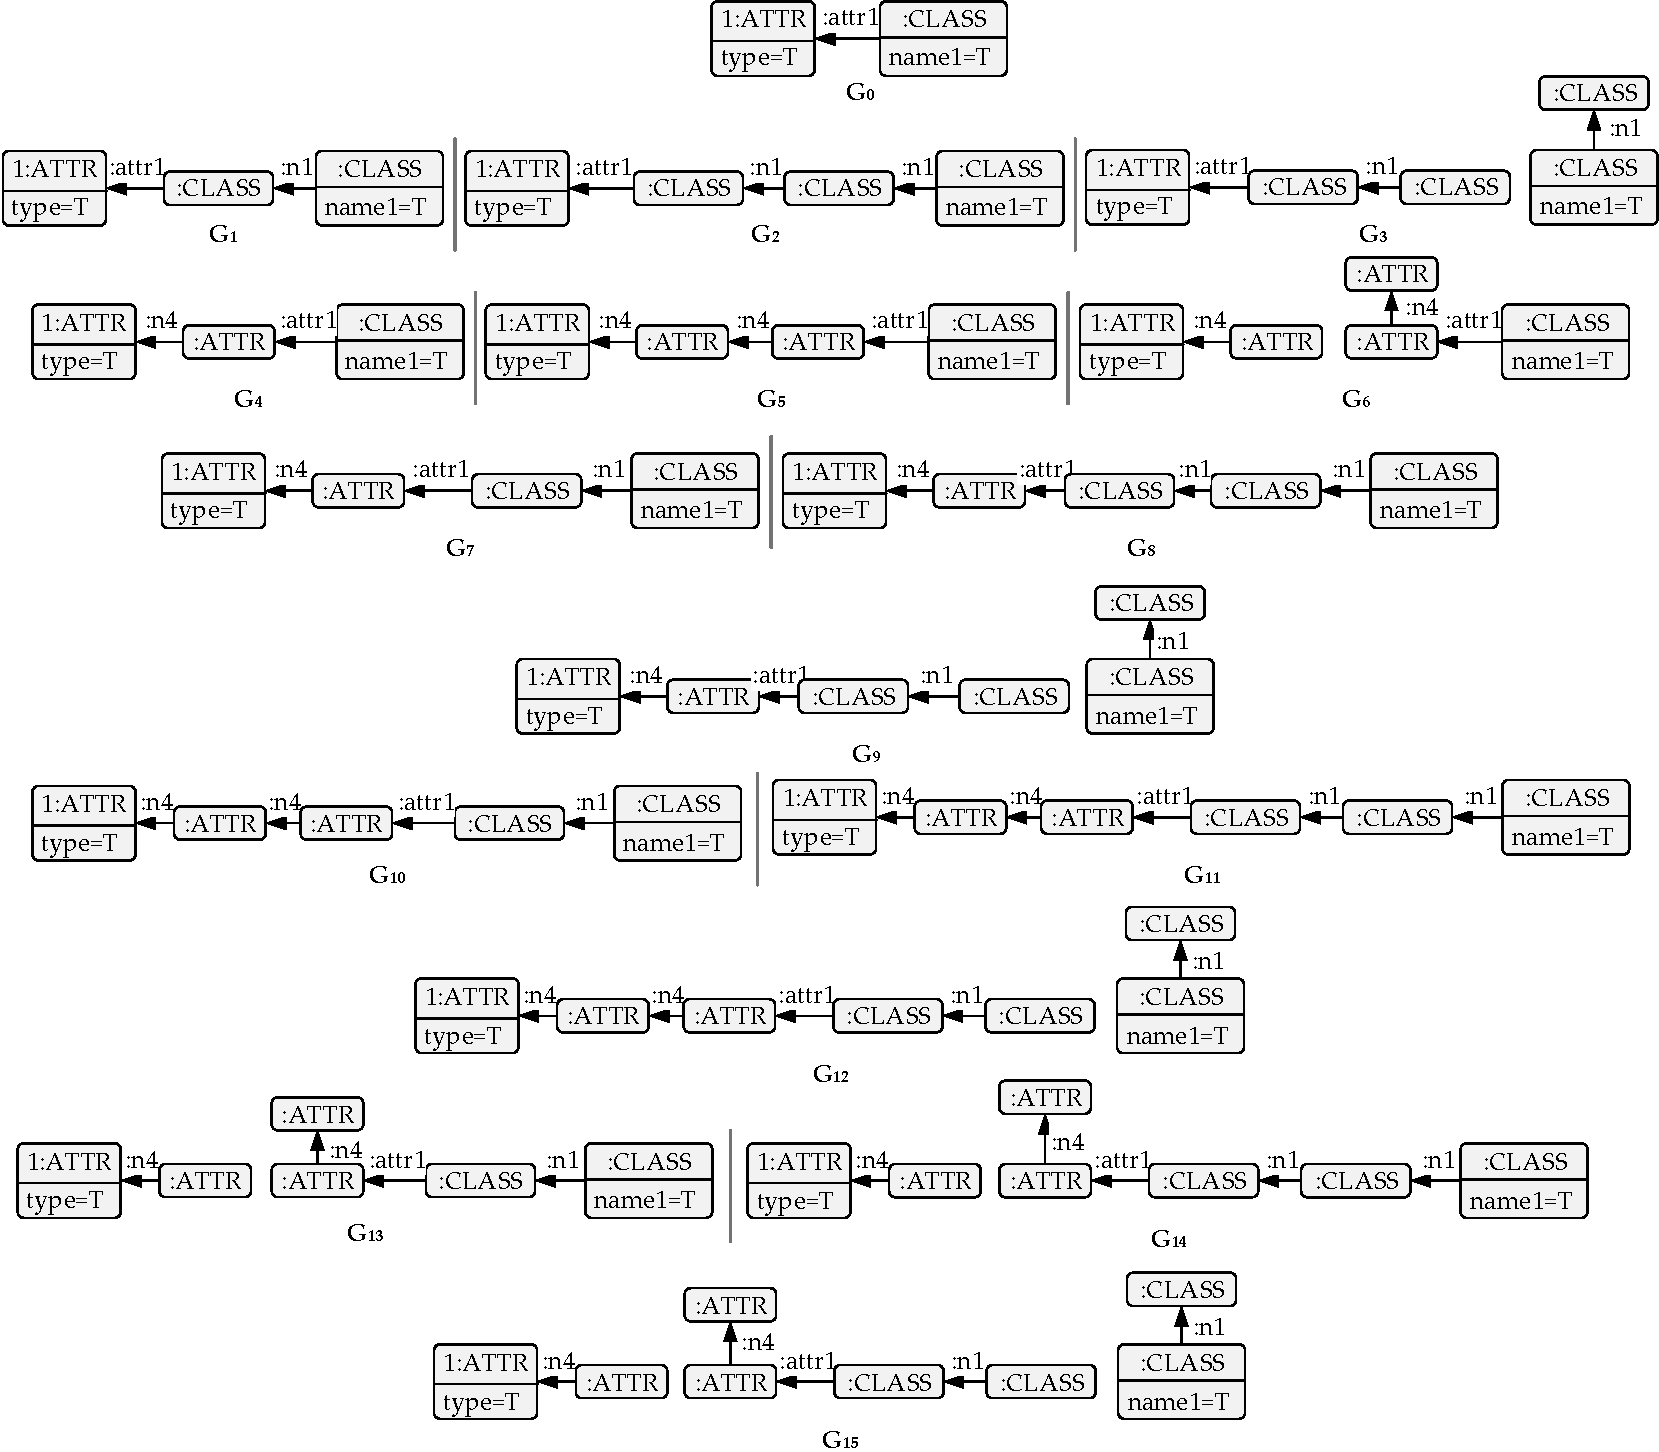
\includegraphics[width=\textwidth]{img/software_trans/wlex.pdf}
\end{center}
\caption{Weakened Graph Language}
\label{fig:sec-compl-software-trans:wglex}
\end{figure}
\end{example}

In the following, we show that the construction of weakened graph languages is well-defined in the sense that it leads to the desired set $\Lang_w(\GS)$ of equivalence classes of morphisms for a given recursive graph schema $\GS$ with start graph $S$.
In particular, 
\begin{enumerate*}
\item \label{item:sec-compl-software-trans:well_def:1}for each acyclic, terminating recursive transformation $t\colon S \Trans{*}_\GS G$ which starts in $S$, there is a class $[\der(t)] \in \Lang_w(\GS)$ that coincides with the derived span $\der(t)$ of $t$,
\item \label{item:sec-compl-software-trans:well_def:2}for each cyclic, terminating recursive transformation $t\colon S \Trans{*}_\GS G$ which starts in $S$, there is a class $[\ac] \in \Lang_w(\GS)$ that may not coincide with but partially reflect $\der(t)$, and
\item \label{item:sec-compl-software-trans:well_def:3}each $[\ac] \in \Lang_w(\GS)$ partially reflects the derived span $\der(t)$ of some terminating recursive transformation $t\colon S \Trans{*}_\GS G$ which starts in $S$.
\end{enumerate*}
We use \cref{item:sec-compl-software-trans:well_def:1,item:sec-compl-software-trans:well_def:2,item:sec-compl-software-trans:well_def:3} for showing that the language over general recursive graph constraints is a subset of the language over weakened recursive graph constraints in \cref{thm:sec-compl-software-trans:comp-lang-constraints} such that domain completeness w.r.t. weakened constraints implies domain completeness w.r.t. general constraints (cf. \cref{thm:sec-compl-software-trans:dom_compl_inf}).
Furthermore, \cref{item:sec-compl-software-trans:well_def:3} illustrates the fact that the weakened language contains (weakened constraints cover) correct cases only which increases the accuracy of the domain completeness verification w.r.t. weakened constraints by potentially omitting the verification of faulty cases.

\begin{proposition}[Well-Definedness of Construction of Weakened Graph Languages]
\label{prop:sec-compl-software-trans:weakened_lang_well_def}
Let $\GS=((S,P),M,s_\GS,t_\GS)$ be a recursive graph schema with non-deleting productions $P$, $\Lang(\GS)$ be the language of $\GS$ and $\Lang_w(\GS)$ be the weakened language of $\GS$.
For the construction of weakened graph languages, the following holds in $\M$-adhesive categories with effective pushouts and initial $\M$-subobjects:\index{recursive graph schema!language!well-definedness}
\begin{enumerate}
\item \label{item:sec-compl-software-trans:well_def_con_w_lan:1}For each terminating, acyclic $t\colon S \Trans{*}_\GS G$ which starts in $S$ there is $[\der(t)] \in \Lang_w(\GS)$,
\item \label{item:sec-compl-software-trans:well_def_con_w_lan:2}For each terminating, cyclic $t\colon S \Trans{*}_\GS G$ which starts in $S$ there is $[\ac\colon S \to G'] \in \Lang_w(\GS)$ such that there is an $\M$-morphism $i\colon G' \to G$ with $i \circ \ac=\der(t)$, and
\item \label{item:sec-compl-software-trans:well_def_con_w_lan:3}For each $[\ac\colon S \to G'] \in \Lang_w(\GS)$ there is terminating $t\colon S \Trans{*}_\GS G$ which starts in $S$ and $\M$-morphism $i\colon G' \to G$ such that $i \circ \ac=\der(t)$.\envEndMarker
\end{enumerate}
\end{proposition}

\begin{proof}
The proof is presented in \cref{sec-proofs:prop:sec-compl-software-trans:weakened_lang_well_def}.
\end{proof}

Based on the notions of tightened and weakened graph languages of recursive graph schemata, we define tightened and weakened recursive graph conditions according to \cref{def:sec-compl-software-trans:sem_rec_cond}.

\begin{definition}[Tightened \& Weakened Recursive Graph Condition]
\label{def:sec-dc-general-rec:t_w_g_constr}
Let $\GS$ be a recursive graph schema.
The recursive graph condition $c_\GS$ w.r.t. $\GS$ is \emph{(tightened w.r.t. a given upper bound $G_u$) weakened}\index{recursive graph condition!tightened}\index{recursive graph condition!weakened}, if it is formed over the (tightened) weakened graph language of $\GS$ (and w.r.t. $G_u$).
\envEndMarker
\end{definition}

\begin{example}[Tightened \& Weakened Recursive Graph Constraint]
The weakened recursive graph condition w.r.t. the recursive graph schema $\GS$ in \cref{ex:sec-compl-software-trans:rec_schema} is given by the disjunction over all morphisms of the corresponding weakened graph language of $\GS$ in \cref{ex:sec-dc-general-rec:weakened_graph_lang}.
Note that the weakened recursive graph constraint is only an approximation to the recursive graph constraint in \cref{ex:sec-compl-software-trans:rec_cond}.
More precisely, it is not required that for all attributes of type $T$ there is a class of name $T$ such that there is a path between both but the path may also be interrupted as illustrated by graphs $G_3,G_6,G_9,G_{12},G_{13},G_{14}$ and $G_{15}$ in \cref{fig:sec-compl-software-trans:wglex}.
In contrast to that, the tightened recursive graph constraint w.r.t. $\GS$ is equivalent to the recursive graph constraint in \cref{ex:sec-compl-software-trans:rec_cond} but only for graphs up to the given upper bound.
\envEndMarker
\end{example}

Analogously to \cref{prop:sec-compl-software-trans:rec_cond_constr_m_norm}, in the following we show that tightened and weakened recursive graph conditions are in $\M$-normal form which is necessary to be used in the verification of domain completeness in \cref{sec-dc-verification,thm:C-extensionCompleteness}.
Furthermore, we investigate the relationship between graph languages over recursive graph constraints in \cref{thm:sec-compl-software-trans:comp-lang-constraints} in order to conclude over the verification of domain completeness w.r.t. infinite graph constraints via \cref{sec-dc-verification,thm:C-extensionCompleteness} in \cref{thm:sec-compl-software-trans:dom_compl_inf}.
More precisely, the verification of domain completeness can be performed w.r.t. tightened \& weakened recursive graph constraints.
While for weakened recursive graph constraints we obtain a general result for domain completeness in \cref{thm:sec-compl-software-trans:dom_compl_inf,thm:sec-compl-software-trans:dom_compl_inf:2}, for tightened recursive graph constraints we obtain a result for domain completeness up to a given upper bound only in \cref{thm:sec-compl-software-trans:dom_compl_inf,thm:sec-compl-software-trans:dom_compl_inf:1}.

\begin{theorem}[Tightened \& Weakened Recursive Graph Conditions in $\M$-normal form]
\label{prop:sec-compl-software-trans:tight_weak_rec_cond_constr_m_norm}
In $\M$-adhesive categories with effective pushouts and initial $\M$-subobjects, \emph{each tightened \& weakened recursive graph condition is in $\M$-normal form}\index{recursive graph condition!tightened!$\M$-normal form}\index{recursive graph condition!weakened!$\M$-normal form}.
\envEndMarker
\end{theorem}

\begin{proof}
Let $\GS$ be a recursive graph schema, $c_\GS$ be the recursive graph condition, $c_{t,\GS}$ be the tightened recursive graph condition and $c_{w,\GS}$ be the weakened recursive graph condition w.r.t. $\GS$.
By \cref{def:sec-dc-general-rec:t_w_g_constr,def:sec-dc-general-rec:t_g_lang} it follows that $c_{t,\GS}$ is built up by a subset of morphisms of $c_\GS$.
Therefore by \cref{prop:sec-compl-software-trans:rec_cond_constr_m_norm} it follows that $c_{t,\GS}$ is in $\M$-normal form.
By \cref{prop:sec-compl-software-trans:weakened_lang_well_def,item:sec-compl-software-trans:well_def_con_w_lan:3}, for each morphism $\ac\colon S \to G'$ in $c_{w,\GS}$, there is a morphism $\der(t)\colon S \to G$ in $c_\GS$ (cf. \cref{def:sec-compl-software-trans:lang_rec,def:sec-compl-software-trans:sem_rec_cond}) and morphism $i \in \M$ such that $i \circ \ac=\der(t)$.
By \cref{prop:sec-compl-software-trans:rec_cond_constr_m_norm}, $\der(t) \in \M$ implying further that $\ac \in \M$ by $\M$-decomposition, i.e., $c_{w,\GS}$ is in $\M$-normal form.
\end{proof}

\begin{proposition}[Relationship between Languages over Recursive Graph Constraints]
\label{thm:sec-compl-software-trans:comp-lang-constraints}
Let $\GS$ be a recursive graph schema with non-deleting productions.
Furthermore, let $c_\GS$ be the recursive graph constraint, and $c_{w,\GS}$ be the weakened recursive graph constraint w.r.t. $\GS$.
Moreover, let $c_{t,\GS}$ be the tightened recursive graph constraint w.r.t. $\GS$ and upper bound $G_u$.
Then, the following holds in $\M$-adhesive categories with effective pushouts and initial $\M$-subobjects:
\begin{enumerate}
  \item $\Lang_I(\{c_\GS\})_{G_u} \subseteq \Lang_I(\{c_{t,\GS}\})$ and $\Lang_I(\{c_\GS\}) \subseteq \Lang_I(\{c_{w,\GS}\})$, and
  \item $\Lang(\{c_\GS\})_{G_u} \subseteq \Lang(\{c_{t,\GS}\})$ and $\Lang(\{c_\GS\}) \subseteq \Lang(\{c_{w,\GS}\})$
\end{enumerate}
where languages $\Lang_I(\{c_\GS\})_{G_u}$ and $\Lang(\{c_\GS\})_{G_u}$ are defined accordingly to \cref{sec-dc-verification,def:sec-dc-verification:dc_ub}.
\envEndMarker
\end{proposition}

\begin{proof}
Let $c_\GS,c_{t,\GS},c_{w,\GS}$ be the corresponding recursive graph constraints over $S$.

\noindent\textbf{Case ($c_{w,\GS}$)}: Let $G \in \Lang_I(\{c_\GS\})$ or $G \in \Lang(\{c_\GS\})$, respectively, and $p\colon S \to G \in \M$ be a corresponding morphism.
By \cref{sec-gt-gc,rem:sec-gc-gc:init_gen_sat} and \cref{sec-dc-general,def:sec-dc-general:lang}, $p \models c_\GS$ $\stackrel{\cref{sec-gt-gc,def:condition-satisfaction}}{\Leftrightarrow} \exists q\colon A \to G \in \M$ for some $\ac\colon S \to A$ in $c_\GS$ such that $q \circ \ac=p$ $\stackrel{\cref{def:sec-compl-software-trans:sem_rec_cond,def:sec-compl-software-trans:lang_rec}}{\Leftrightarrow} \exists q\colon A \to G \in \M$ for some $\der(t)=\ac\colon S \to A$ with $t\colon S \Trans{*}_\GS A$ being terminating and starting in $S$ such that $q \circ \der(t)=p$ $\stackrel{\cref{prop:sec-compl-software-trans:weakened_lang_well_def,item:sec-compl-software-trans:well_def_con_w_lan:1,item:sec-compl-software-trans:well_def_con_w_lan:2}\text{ and }\cref{def:sec-dc-general-rec:t_w_g_constr}}{\Rightarrow} \exists q\colon A \to G \in \M,\ac'\colon S \to A'$ in $c_{w,\GS}$, and $i\colon A' \to A \in \M$ such that $i \circ \ac'=\der(t)$ implying further that $\exists q \circ i\colon A' \to G \in \M$ for $\ac'\colon S \to A'$ in $c_{w,\GS}$ by $\M$-composition $\stackrel{\cref{sec-gt-gc,def:condition-satisfaction}}{\Leftrightarrow} p \models c_{w,\GS}$.
Therefore by \cref{sec-gt-gc,rem:sec-gc-gc:init_gen_sat}, $G \stackrel{I}{\models} c_{w,\GS}$ or $G \models c_{w,\GS}$, respectively, implying further that $G \in \Lang_I(\{c_{w,\GS}\})$ or $G \in \Lang(\{c_{w,\GS}\})$, respectively, by \cref{sec-dc-general,def:sec-dc-general:lang}.

\noindent\textbf{Case ($c_{t,\GS}$)}: Let $G \in \Lang_I(\{c_\GS\})_{G_u}$ or $G \in \Lang(\{c_\GS\})_{G_u}$, respectively, and $p\colon S \to G \in \M$ be a corresponding morphism.
By \cref{sec-dc-verification,def:sec-dc-verification:dc_ub}, $G \in \Lang_I(\{c_\GS\})$ or $G \in \Lang(\{c_\GS\})$, respectively, and furthermore, there is $i\colon G \to G_u \in \M$.
By \cref{sec-gt-gc,rem:sec-gc-gc:init_gen_sat} and \cref{sec-dc-general,def:sec-dc-general:lang}, $p \models c_\GS$ $\stackrel{\cref{sec-gt-gc,def:condition-satisfaction}}{\Leftrightarrow} \exists q\colon A \to G \in \M$ for some $\ac\colon S \to A$ in $c_\GS$ such that $q \circ \ac=p$.
Thus, by $\M$-composition there is $i \circ q\colon A \to G_u \in \M$ implying further that $\ac$ is a morphism in $c_{t,\GS}$ by \cref{def:sec-dc-general-rec:t_g_lang,def:sec-dc-general-rec:t_w_g_constr}, i.e., $p \models c_{t,\GS}$.
Therefore by \cref{sec-gt-gc,rem:sec-gc-gc:init_gen_sat}, $G \stackrel{I}{\models} c_{t,\GS}$ or $G \models c_{t,\GS}$, respectively, implying further that $G \in \Lang_I(\{c_{t,\GS}\})$ or $G \in \Lang(\{c_{t,\GS}\})$, respectively, by \cref{sec-dc-general,def:sec-dc-general:lang}.
\end{proof}

\begin{theorem}[Verification of Domain Completeness w.r.t. Recursive Graph Constraints]
\label{thm:sec-compl-software-trans:dom_compl_inf}
Let $\GG$ be a grammar, $\overline{\GS}$ be a set of recursive graph schemata with non-deleting productions, $C_{\overline{\GS}}$ be the set of recursive graph constraints, and $C_{w,\overline{\GS}}$ be the set of weakened recursive graph constraints w.r.t. $\overline{\GS}$.
Furthermore, let $C_{t,\overline{\GS}}$ be the set of tightened recursive graph constraints w.r.t. $\overline{\GS}$ and a common upper bound $G_u$.
Then, the following holds in $\M$-adhesive categories with effective pushouts and initial $\M$-subobjects for a given set of constraints $C$:
\begin{enumerate}
  \item \label{thm:sec-compl-software-trans:dom_compl_inf:1}$\Lang(C \cup C_{t,\overline{\GS}}) \subseteq \Lang(\GG)$ implies domain completeness up to upper bound $G_u$: $\Lang(C \cup C_{\overline{\GS}})_{G_u} \subseteq \Lang(\GG)$, and
  \item \label{thm:sec-compl-software-trans:dom_compl_inf:2}$\Lang(C \cup C_{w,\overline{\GS}}) \subseteq \Lang(\GG)$ implies domain completeness: $\Lang(C \cup C_{\overline{\GS}}) \subseteq \Lang(\GG)$.
  \envEndMarker
\end{enumerate}
\end{theorem}

\begin{proof}
\begin{enumerate}
  \item We assume $\Lang(C \cup C_{t,\overline{\GS}}) \subseteq \Lang(\GG)$.
  Let $G \in \Lang(C \cup C_{\ol{\GS}})_{G_u}$ with $C=C_I \cup C_G$ and $C_{\ol{\GS}}=C_{I,\ol{\GS}} \cup C_{G,\ol{\GS}}$ where constraints $C_I,C_{I,\ol{\GS}}$ are designated for initial satisfaction and $C_G,C_{G,\ol{\GS}}$ are designated for general satisfaction
  $\stackrel{\cref{sec-dc-verification,def:sec-dc-verification:dc_ub}}{\Leftrightarrow} G \in \Lang(C \cup C_{\ol{\GS}})$ and $\exists i\colon G \to G_u \in \M$
  $\stackrel{\cref{sec-dc-general,def:sec-dc-general:lang}}{\Leftrightarrow} G \in \Lang_I(C_I \cup C_{I,\ol{\GS}})$ and $G \in \Lang(C_G \cup C_{G,\ol{\GS}})$, i.e., $G \stackrel{I}{\models} C_I \cup C_{I,\ol{\GS}}$ and $G \models C_G \cup C_{G,\ol{\GS}}$ and $\exists i\colon G \to G_u \in \M$
  $\stackrel{\cref{sec-gt-gc,def:constr_sat}\text{ and }\cref{sec-dc-general,def:sec-dc-general:lang}}{\Rightarrow} G \in \Lang_I(C_I)$, $\forall c_\GS \in C_{I,\ol{\GS}}.G \in \Lang_I(\{c_\GS\})$ $,G \in \Lang(C_G)$, and $\forall c_\GS \in C_{G,\ol{\GS}}.G \in \Lang(\{c_\GS\})$ and $\exists i\colon G \to G_u \in \M$
  $\stackrel{\cref{sec-dc-verification,def:sec-dc-verification:dc_ub}}{\Rightarrow}$ $G \in \Lang_I(C_I)$, $\forall c_\GS \in C_{I,\ol{\GS}}.G \in \Lang_I(\{c_\GS\})_{G_u}$ $,G \in \Lang(C_G)$, and $\forall c_\GS \in C_{G,\ol{\GS}}.G \in \Lang(\{c_\GS\})_{G_u}$
  $\stackrel{\cref{thm:sec-compl-software-trans:comp-lang-constraints}}{\Rightarrow}$ $G \in \Lang_I(C_I)$, $\forall c_\GS \in C_{I,\ol{\GS}}.G \in \Lang_I(\{c_{t,\GS}\})$ $,G \in \Lang(C_G)$, and $\forall c_\GS \in C_{G,\ol{\GS}}.G \in \Lang(\{c_{t,\GS}\})$ with $c_{t,\GS} \in C_{t,\ol{\GS}}$
  $\stackrel{\cref{sec-gt-gc,def:constr_sat}\text{ and }\cref{sec-dc-general,def:sec-dc-general:lang}}{\Rightarrow}$ $G \in \Lang(C)$ and $G \in \Lang(C_{t,\ol{\GS}})$
  $\Rightarrow G \in \Lang(C \cup C_{t,\ol{\GS}})$
  $\stackrel{Assumption}{\Rightarrow}$ $G \in \Lang(\GG)$.
  \item We assume $\Lang(C \cup C_{w,\overline{\GS}}) \subseteq \Lang(\GG)$.
  Let $G \in \Lang(C \cup C_{\ol{\GS}})$ with $C=C_I \cup C_G$ and $C_{\ol{\GS}}=C_{I,\ol{\GS}} \cup C_{G,\ol{\GS}}$ where constraints $C_I,C_{I,\ol{\GS}}$ are designated for initial satisfaction and $C_G,C_{G,\ol{\GS}}$ are designated for general satisfaction
  $\stackrel{\cref{sec-dc-general,def:sec-dc-general:lang}}{\Leftrightarrow} G \in \Lang_I(C_I \cup C_{I,\ol{\GS}})$ and $G \in \Lang(C_G \cup C_{G,\ol{\GS}})$, i.e., $G \stackrel{I}{\models} C_I \cup C_{I,\ol{\GS}}$ and $G \models C_G \cup C_{G,\ol{\GS}}$
  $\stackrel{\cref{sec-gt-gc,def:constr_sat}\text{ and }\cref{sec-dc-general,def:sec-dc-general:lang}}{\Rightarrow} G \in \Lang_I(C_I)$, $\forall c_\GS \in C_{I,\ol{\GS}}.G \in \Lang_I(\{c_\GS\})$ $,G \in \Lang(C_G)$, and $\forall c_\GS \in C_{G,\ol{\GS}}.G \in \Lang(\{c_\GS\})$
  $\stackrel{\cref{thm:sec-compl-software-trans:comp-lang-constraints}}{\Rightarrow}$ $G \in \Lang_I(C_I)$, $\forall c_\GS \in C_{I,\ol{\GS}}.G \in \Lang_I(\{c_{w,\GS}\})$ $,G \in \Lang(C_G)$, and $\forall c_\GS \in C_{G,\ol{\GS}}.G \in \Lang(\{c_{w,\GS}\})$ with $c_{w,\GS} \in C_{w,\ol{\GS}}$
  $\stackrel{\cref{sec-gt-gc,def:constr_sat}\text{ and }\cref{sec-dc-general,def:sec-dc-general:lang}}{\Rightarrow}$ $G \in \Lang(C)$ and $G \in \Lang(C_{w,\ol{\GS}})$
  $\Rightarrow G \in \Lang(C \cup C_{w,\ol{\GS}})$
  $\stackrel{Assumption}{\Rightarrow}$ $G \in \Lang(\GG)$.
\end{enumerate}
\end{proof}

Finally, we show that tightened and weakened recursive graph constraints can effectively be used for verifying domain completeness.
This means that the constraints are actually finite under certain conditions such that the verification terminates (cf. \cref{th:sec-dc-verification:term_dc,thm:sec-compl-software-trans:fin_rec_gc}).
Note that the number of nestings of recursive graph constraints is finite by constructions \cref{def:sec-compl-software-trans:sem_rec_cond,def:sec-dc-general-rec:t_w_g_constr}.
For ensuring the finiteness of weakened recursive graph constraints, we introduce the notion of simple recursive graph schemata in \cref{def:sec-dc-general-rec:simple_rec_gr_schema}.
A recursive graph schema is simple if all acyclic match-cycles that are not equal up to shifting of matches are linked via at most one production as depicted in \cref{fig:sec-dc-general-rec:simple_rec_schema} (a).
The schemata in \cref{fig:sec-dc-general-rec:simple_rec_schema} (b) and (c) are not simple.
\cref{fig:sec-dc-general-rec:simple_rec_schema} (b) contains two acyclic match-cycles \code{(1)} and \code{(2)} that are linked via two productions.
\cref{fig:sec-dc-general-rec:simple_rec_schema} (c) contains a cycle of acyclic match-cycles \code{(1)}, \code{(2)} and \code{(3)} that are linked to each other via one production, respectively.
However, this situation always leads to an acyclic match-cycle \code{(4)} which is linked to other match-cycles via more than one production. 
Therefore, a cycle of acyclic match-cycles is also forbidden for simple recursive graph schemata.

\begin{figure}[!tb]
\begin{center}
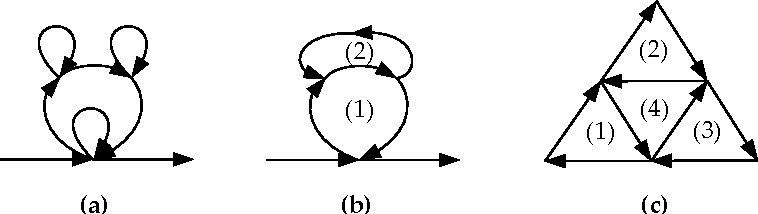
\includegraphics[width=.75\textwidth]{img/software_trans/simple.pdf}
\end{center}
\caption{Simple Recursive Graph Schema}
\label{fig:sec-dc-general-rec:simple_rec_schema}
\end{figure}

\begin{definition}[Simple Recursive Graph Schema]
\label{def:sec-dc-general-rec:simple_rec_gr_schema}
\index{recursive graph schema!simple}
Let $\GS$ be a recursive graph schema and $\quotient{\Paths_{\_,\_}(\GS)}{\sim}$ be the equivalence classes of all acyclic match-cycles in $\GS$ that are equal up to shifting of matches as defined in \cref{def:sec-dc-general-rec:equ_match_cycles}.
Then $\GS$ is simple, if for all $[\paths_1],[\paths_2] \in \quotient{\Paths_{\_,\_}(\GS)}{\sim}$ and for all $m_i,m_{i'} \in \paths_1$ and $m_j,m_{j'} \in \paths_2$ it holds that $s_\GS(m_i)=s_\GS(m_j)$ and $s_\GS(m_{i'})=s_\GS(m_{j'})$ implies that $m_i=m_{i'}$ and $m_j=m_{j'}$.
\envEndMarker
\end{definition}

\begin{example}[Simple Recursive Graph Schema]
The recursive graph schema in \cref{fig:sec-compl-software-trans:rec_graph} is simple while the schema in \cref{fig:sec-compl-software-trans:rec_graph_schema2} is not simple.
\envEndMarker
\end{example}

\begin{theorem}[Finiteness of Recursive Graph Constraints]
\label{thm:sec-compl-software-trans:fin_rec_gc}
Let $\GS=((S,P),M,s_\GS,t_\GS)$ be a recursive graph schema.
\begin{enumerate}
  \item The recursive graph constraint $c_\GS$ w.r.t. $\GS$ is finite, if:
  \begin{enumerate}
    \item \label{thm:sec-compl-software-trans:fin_rec_gc:1}The set $\Paths_S(\GS)$ of acyclic, terminating match-paths in $\GS$ that start in $S$ is finite, and 
    \item \label{thm:sec-compl-software-trans:fin_rec_gc:2}For all match-paths $\paths \in \Paths_S(\GS)$ there is no match-cycles in $\GS$ that is reachable from $\paths$.
  \end{enumerate}
  \item In $(\AGraphs_\ATGI,\M)$, the tightened recursive graph constraint $c_{t,\GS}$ w.r.t. $\GS$ and upper bound $G_u$ is finite, if:
  \begin{enumerate}
    \item \label{thm:sec-compl-software-trans:fin_rec_gc:5}Recursive graph schema $\GS$ contains non-deleting productions $P$ only,
    \item \label{thm:sec-compl-software-trans:fin_rec_gc:3}Graph $G_u$ is finite, and
    \item \label{thm:sec-compl-software-trans:fin_rec_gc:4}The set of matches $M$ is finite.
  \end{enumerate}
  \item In $(\AGraphs_{\ATGI,\fin},\M_\fin)$, the weakened recursive graph constraint $c_{w,\GS}$ w.r.t. $\GS$ is finite, if:
  \begin{enumerate}
    \item \label{thm:sec-compl-software-trans:fin_rec_gc:6}The set of matches $M$ is finite, and
    \item \label{thm:sec-compl-software-trans:fin_rec_gc:7}Recursive graph schema $\GS$ is simple.
    \envEndMarker
  \end{enumerate}
\end{enumerate}
\end{theorem}

\begin{proof}
By \cref{sec-gt-gc,def:condition-satisfaction}, for constraint $c$ is finite we have to show that the index set $I$ of every disjunction $\vee_{i \in I}$ in $c$ is finite.
\begin{enumerate}
  \item By assumptions \cref{thm:sec-compl-software-trans:fin_rec_gc,thm:sec-compl-software-trans:fin_rec_gc:1,thm:sec-compl-software-trans:fin_rec_gc:2} and \cref{def:sec-compl-software-trans:lang_rec}, language $\Lang(\GS)$ of $\GS$ is the finite set of derived spans of the finite set of terminating recursive transformation sequences starting at $S$.
  Thus, by construction \cref{def:sec-compl-software-trans:sem_rec_cond}, $c_\GS$ is finite.
  \item W.l.o.g. and by assumption \cref{thm:sec-compl-software-trans:fin_rec_gc,thm:sec-compl-software-trans:fin_rec_gc:5} we assume that each recursive transformation step via a production $p \in P$ and match $m \in M$ creates at least one graph element while preserving the remaining elements.
  By $M$ being finite by assumption \cref{thm:sec-compl-software-trans:fin_rec_gc,thm:sec-compl-software-trans:fin_rec_gc:4}, we have finitely many possibilities at each step to continue with the next step until we have exceeded finite upper bound $G_u$ (cf. assumption \cref{thm:sec-compl-software-trans:fin_rec_gc,thm:sec-compl-software-trans:fin_rec_gc:3}).
  Therefore, there are finitely many recursive transformation sequences up to upper bound $G_u$ leading to finitely many derived spans in tightened language $\Lang_t(\GS,G_u)$ of $\GS$ and w.r.t. $G_u$ (cf. \cref{def:sec-dc-general-rec:t_g_lang}).
  Thus, by construction \cref{def:sec-dc-general-rec:t_w_g_constr}, $c_{t,\GS}$ is finite.
  \item We focus on the construction of weakened languages in \cref{def:sec-compl-software-trans:weakened_lang}.
  There are at most $|M|!$ acyclic match-paths in $\GS$, each consisting of at most $|M|$ matches, since, having a match $m \in M$ two-times in a path yields a cyclic path.
  Therefore by assumption \cref{thm:sec-compl-software-trans:fin_rec_gc,thm:sec-compl-software-trans:fin_rec_gc:6} of $M$ being finite, the set of acyclic match-paths in $\GS$ is finite and furthermore, each acyclic match-path consists of a finite set of matches.
  Thus, the set $\underline{\Paths}_S(\GS)$ of acyclic, terminating match-paths in $\GS$ that start in $S$ is finite.
  Analogously, the set $\mathcal{P}$ of acyclic match-cycles in $\GS$ that are equal up to shifting of matches is finite.
  Therefore, we can iterate over all paths $m \in \underline{\Paths}_S(\GS)$ and call $\underline{\Lang}_w$, respectively.
  In each call for $\underline{\Lang}_w(m,1,\id,\id,1)$ we can iterate over the finite set of matches $m_i \in m$ if $\mathcal{P}=\varnothing$ for each $m_i \in m$.
  If for some $m_i \in m$, $\mathcal{P} \neq \varnothing$, then we can iterate over finite $\mathcal{P}$ and the finite set of overlappings $(A \oplus B_\paths)$ in $\mathcal{C}$ with recursive calls of $\underline{\Lang}_w(\paths,1,\id,\id,2)$ for each $\paths \in \mathcal{P}$, since, we are in category $(\AGraphs_{\ATGI,\fin},\M_\fin)$ of finite graphs and therefore, the set of possible overlappings is finite.
  Analogously, we conclude for all recursive calls and furthermore, the recursion is guaranteed to end at depth $|M|!$ for each case, since, $\GS$ is simple by assumption \cref{thm:sec-compl-software-trans:fin_rec_gc,thm:sec-compl-software-trans:fin_rec_gc:7}.
  Thus, set $\mathcal{C}$ is finite in each case.
  In conclusion, the weakened language $\Lang_w(\GS)$ of $\GS$ is a finite set of morphisms implying that the weakened recursive graph constraint $c_{w,\GS}$ w.r.t. $\GS$ is finite by \cref{def:sec-dc-general-rec:t_w_g_constr}.
\end{enumerate}
\end{proof}

Note that weakened constraints involve additional approximations -- A graph up to an upper bound satisfies the original constraint if and only if it satisfies the tightened constraint. However, a graph satisfies the weakened constraint if it satisfies the original constraint but not necessarily vice versa.
Thus, verifying domain completeness against weakened constraints my involve more graphs than verifying against the original constraints.
Therefore, verifying domain completeness w.r.t. tightened constraints may be more accurate and lead to less false negatives in comparison to a verification w.r.t. weakened constraints when having an upper bound for the size of graphs.
On the other hand, verifying domain completeness w.r.t. weakened constraints yields a more general result without an upper bound and may be more efficient, since, not all possibilities of cyclic match-paths up to a certain upper bound are listed in weakened constraints and therefore, must not be checked.

\section{Domain Restrictions}
\label{sec-dc-general-res}
\begin{figure}[!tb]
\begin{center}
\begin{tikzpicture}[]
\fill (0,0) node[inner sep=1pt] (A) {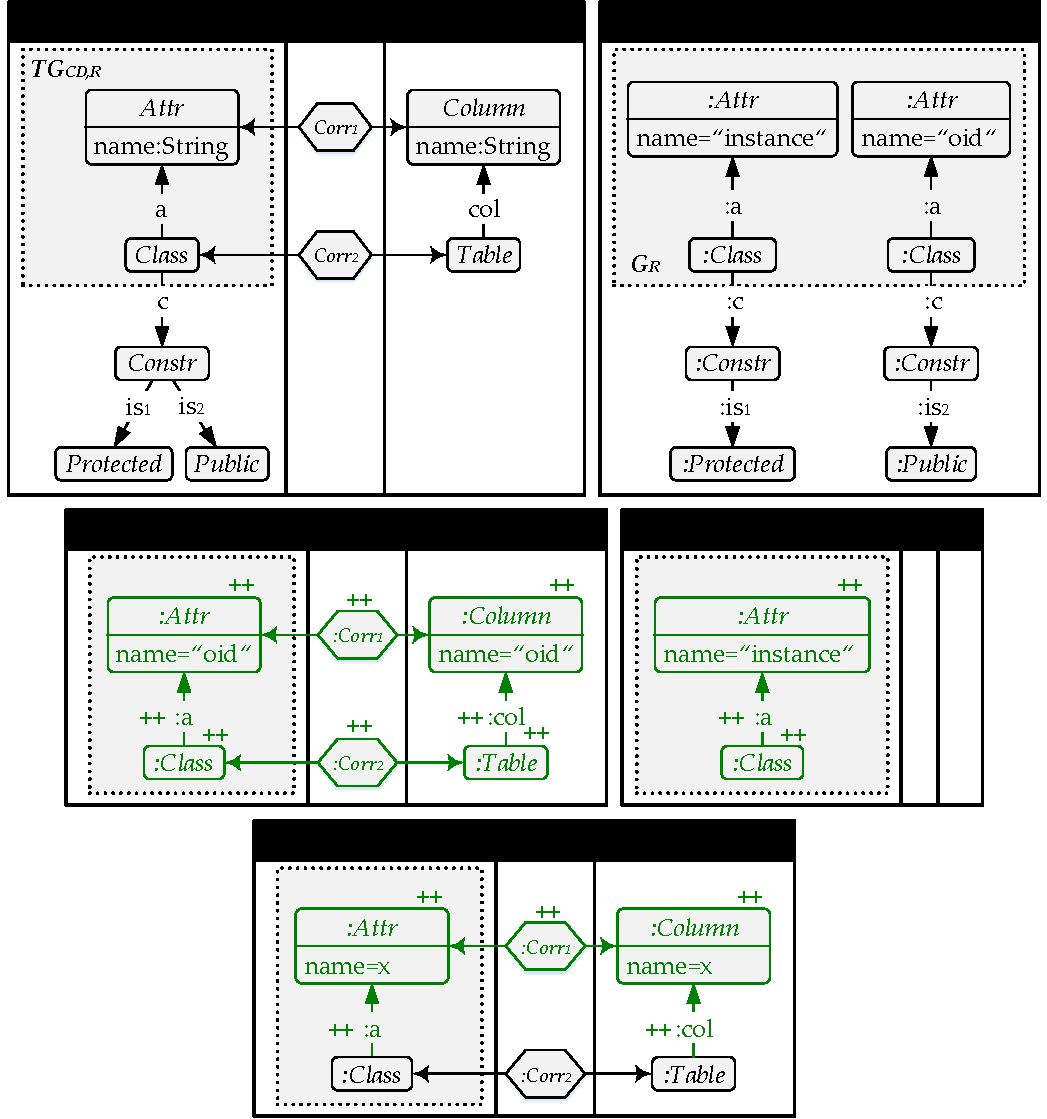
\includegraphics[width=\textwidth]{img/domain_res/res_tg.pdf}};
\fill (-2.5,7.55) node[inner sep=1pt] (B) {\textcolor{white}{$(\TG_\CD \gets \Corr \to \TG_\RDBM)$}};
\fill (1.4,7.55) node[inner sep=1pt] (C) {\textcolor{white}{$G$}};
\fill (-4.35,.4) node[inner sep=1pt] (D) {\textcolor{white}{InstantiableClass2Table}};
\fill (3,.4) node[inner sep=1pt] (E) {\textcolor{white}{Singleton2Empty}};
\fill (-2.55,-3.95) node[inner sep=1pt] (F) {\textcolor{white}{Attr2Column}};
\end{tikzpicture}
\end{center}
\caption{Triple Type Graph $(\TG_\CD \gets \Corr \to \TG_\RDBM)$ with Domain Restriction $\TG_{\CD,R}$ (top,left), Graph $G$ with Resitriction $G_R$ (top,right) and Triple Rules (bottom)}
\label{fig:sec-dc-general:res_tg}
\end{figure}

\begin{figure}[!tb]
\begin{center}
\begin{tikzpicture}[]
\fill (0,0) node[inner sep=1pt] (A) {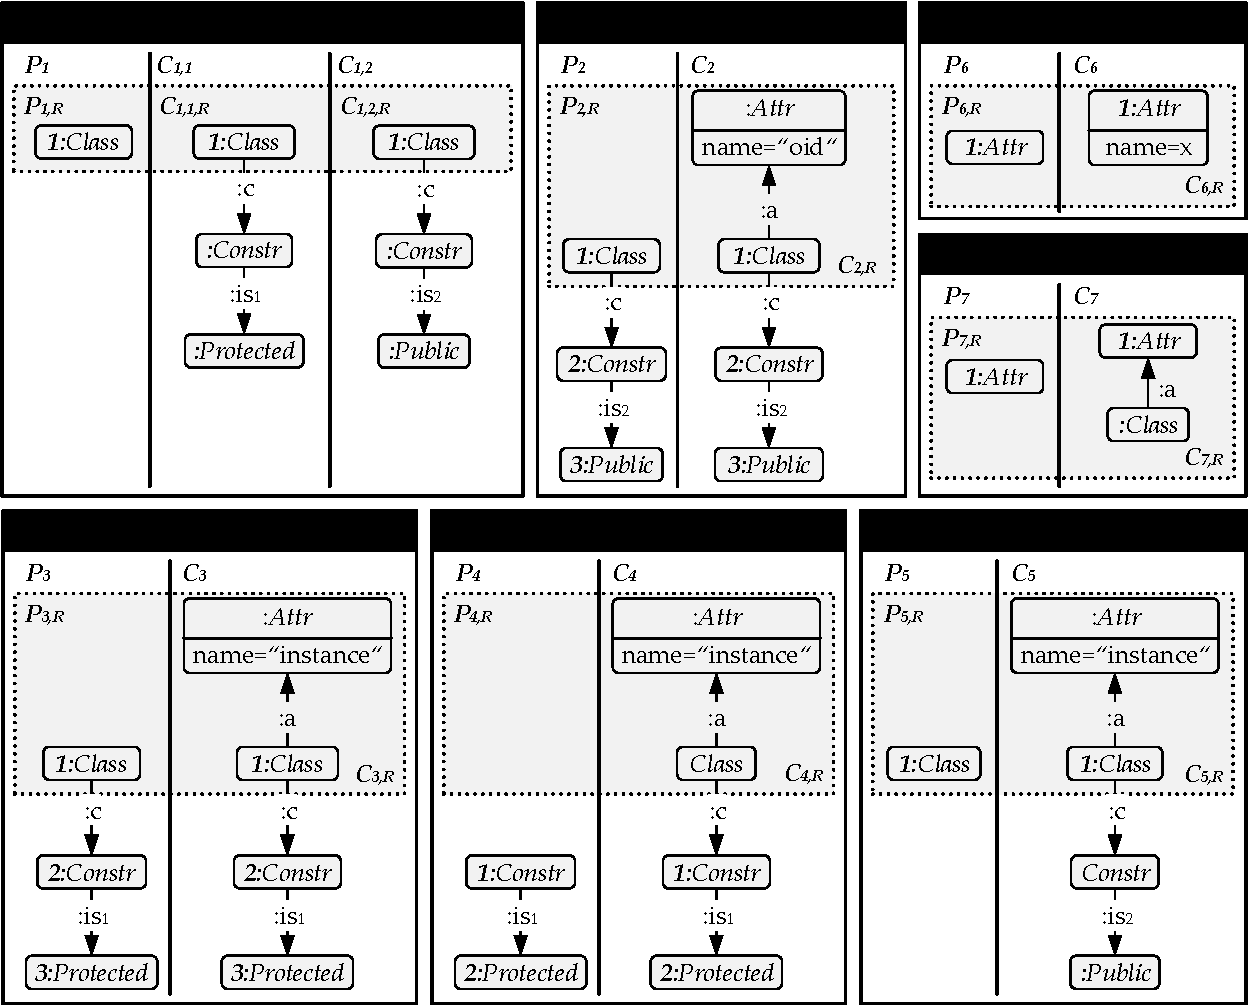
\includegraphics[width=\textwidth]{img/domain_res/res_c.pdf}};
\fill (-4.6,5.65) node[inner sep=1pt] (B) {\textcolor{white}{$c_1=\vee_{i=(1,2)}(\exists(P_1 \to C_{1,i},\true))$}};
\fill (.9,5.65) node[inner sep=1pt] (C) {\textcolor{white}{$c_2=\exists(P_2 \to C_2,\true)$}};
\fill (-5.45,-.35) node[inner sep=1pt] (D) {\textcolor{white}{$c_3=\exists(P_3 \to C_3,\true)$}};
\fill (-.4,-.35) node[inner sep=1pt] (E) {\textcolor{white}{$c_4=\exists(P_4 \to C_4,\true)$}};
\fill (4.8,-.35) node[inner sep=1pt] (F) {\textcolor{white}{$c_5=\neg\exists(P_5 \to C_5,\true)$}};
\fill (5.4,5.65) node[inner sep=1pt] (G) {\textcolor{white}{$c_6=\exists(P_6 \to C_6,\true)$}};
\fill (5.4,2.9) node[inner sep=1pt] (H) {\textcolor{white}{$c_7=\exists(P_7 \to C_7,\true)$}};
\end{tikzpicture}
\end{center}
\caption{Domain Graph Constraints with Restrictions}
\label{fig:sec-dc-general:res_c}
\end{figure}

According to \cref{sec-dom-compl}, we assume that the graphs (models) in the domain of discourse are defined by a domain type graph together with a set $C$ of domain graph constraints.
When verifying domain completeness w.r.t. a given graph grammar $\GG$, we may not be interested in a complete coverage of language $\Lang(C)$ by language $\Lang(\GG)$ but only in the coverage of certain elements of each graph in $\Lang(C)$ by $\Lang(\GG)$ which we call domain completeness under restrictions.
In \cref{fig:sec-dc-general:res_tg} we adress the translation of UML class diagrams (CDs) into relational database models (RDBMs) based on a triple graph grammar (TGG) (cf. \cref{sec-gen-intro-trafos}).
Therefore, the translation (TGG) only covers those elements $\TG_{\CD,R}$ in class diagrams that are related to RDBMs, i.e., classes and their attributes, while neglecting other details concerning class constructors and their visibilities.
However, the graph constraints restricting the structures of class diagrams may not only cover RDBM related elements but also other irrelevant elements for the translation.
This is problematic when verifying domain completeness under restrictions based on the techniques for verifying domain completeness in \cref{sec-dc-verification}, since, the extension of graphs via the constraints may lead to graphs with irrelevant elements that cannot be covered by the TGG causing the verification of $C$-extension completeness in \cref{def:C-extensionCompleteness} to fail.
In \cref{thm:sec-dc-general-res:dom_compl_res}, we give sufficient conditions under which the constraints can be restricted to relevant elements such that domain completeness under restrictions w.r.t. the original constraints can be verified based on the techniques for verifying domain completeness w.r.t. the restricted constraints in the sense of \cref{sec-dc-verification}.

\paragraph*{General Assumption:}
Initial and general satisfaction of constraints are defined over an initial object (cf. \cref{def:constr_sat}).
Therefore, we assume that the results of this Section are applied in the context of $\M$-adhesive categories with initial object.
Moreover, for the extension of constraints in \cref{thm:sec-dc-general-res:ext_constr}, we assume $\M$-adhesive categories with effective pushouts.

\paragraph*{}
For example, the triple type graph $(\TG_\CD \gets \Corr \to \TG_\RDBM)$ in \cref{fig:sec-dc-general:res_tg} (top,left) defines the model elements of class diagrams and database models.
Class diagrams (type graph $\TG_\CD$) may contain several \code{Class}es where each class may have an arbitrary number of \code{Attr}ibutes, each with a specific \code{name} of type \code{String}.
Furthermore, each class may have a \code{Constr}uctor with visibility \code{Protected} or \code{Public}.
Classes with protected constructors are singleton classes, i.e., there exists exactly one instance of each class.
In contrast, classes with public constructors are instantiable classes, i.e., there may exist an arbitrary number of instances of each class.
On the other hand, RDBMs (type graph $\TG_\RDBM$) may contain several \code{Table}s, each with an arbitrary number of \code{Column}s with a specific \code{name} of type \code{String}.
Moreover, classes (attributes) in CDs correspond to tables (columns) in RDBMs via $\Corr_2$ ($\Corr_1$) (cf. type graph $\Corr$).

Furthermore, the constraints in \cref{fig:sec-dc-general:res_c} state that
\begin{enumerate*}
\item each \code{Class} has a \code{Constr}uctor of visibility \code{Protected} or \code{Public} ($c_1=\vee_{i=(1,2)}(\exists(P_1 \to C_{1,i},\true))$),
\item each instantiable class has an \code{Attr}ibute ``\code{oid}'' (object id) which contains the unique id for each instantiated object of the class ($c_2=\exists(P_2 \to C_2,\true)$),
\item each singleton class has an attribute ``\code{instance}'' which contains the singleton instance object of the class ($c_3=\exists(P_3 \to C_3,\true)$),
\item each protected constructor is the constructor of some class with attribute ``instance'' ($c_4=\exists(P_4 \to C_4,\true)$ - Analogously, for public constructors a similar constraint is defined with attribute ``oid''),
\item each class is either singleton or instantiable, i.e., for each class there does not exist a public constructor and an attribute ``instance'' at the same time ($c_5=\neg\exists(P_5 \to C_5,\true)$ - Analogously, a similar constraint is defined for the combination of protected constructor and attribute ``oid''),
\item each attribute has a \code{name} ($c_6=\exists(P_6 \to C_6,\true)$), and
\item each attribute is assigned to a class ($c_7=\exists(P_7 \to C_7,\true)$).
\end{enumerate*}
Moreover, a constraint may be defined that prohibits classes to have protected and public constructors at the same time.

The triple rule \code{InstantiableClass2Table} in \cref{fig:sec-dc-general:res_tg} (bottom) defines the translation from CDs into RDBMs by mapping instantiable \code{Class}es with \code{Attr}ibute \code{oid} in CDs to corresponding \code{Table}s with \code{Column} \code{oid} in RDBMs.
Triple rule \code{Singleton2Empty} maps singleton \code{Classes} with \code{Attr}ibute \code{instance} in CDs to nothing in RDBMs, i.e., only instantiable classes are translated to corresponding tables whereas singleton classes are omitted.
Finally, triple rule \code{Attr2Column} translates general \code{Attr}ibutes with \code{name} ``\code{x}'' of \code{Class}es in CDs into \code{Columns} with the same name ``\code{x}" of corresponding \code{Table}s in RDBMs.

Therefore, the translation is restricted to (only covers) classes and attributes in CDs while neglecting constructors and their visibilities.
According to \cite{DBLP:journals/corr/abs-1209-1436}, the restriction is formalised by an $\M$-type morphism $t\colon \TG_{\CD,R} \to \TG_\CD \in \M$ from the restricted type graph $\TG_{\CD,R}$ which only contains classes and their attributes to the complete domain type graph $\TG_\CD$ of class diagrams (cf. \cref{fig:sec-dc-general:res_tg} (top,left)).
Therefore, each graph and graph constraint can be restricted along the type morphism while both may also contain elements outside the restriction, in general.
For example, graph $G_R$ in \cref{fig:sec-dc-general:res_tg} (top,right) is the restriction of graph $G$ along type morphism $t$ and constraints $c_i[P_i \mapsto P_{i,R},C_i \mapsto C_{i,R}]$ in \cref{fig:sec-dc-general:res_c} where premise (conclusion) $P_i$ ($C_i$) is substituted by $P_{i,R}$ ($C_{i,R}$) in each constraint are the restrictions of constraints $(c_i)_{i=(1..6)}$ along $t$.
The domain completeness problem under restrictions w.r.t. a given set of domain graph constraints $C$ and a graph grammar $\GG$ is as follows: Given a restriction of the domain type graph, does it hold for each graph $G$ in $\Lang(C)$ that the restriction of $G$ which comprises relevant elements only (i.e., elements that are typed over the restricted type graph) is covered by (contained in) grammar $\GG$ (language $\Lang(\GG)$)?

In the following, we first recall the definitions for rectrictions of graphs and positive (nested) graph constraints along type morphisms from \cite{DBLP:journals/corr/abs-1209-1436} and then we define the domain completeness problem under restrictions in accordance with the general domain completeness problem from \cref{def:sec-dc-general:dcp}.

%\vspace{2ex}
\parpic[r][r]{
\SelectTips{cm}{}
$
\xymatrix@C-4ex@R-4ex{
\TG & & G \ar[ll]_{t_G} & & G' \ar[ll]_{a} \\
& & & & \\
& (1) & & (2) & \\
& & & & \\
\TG_R \ar[uuuu]^{t} & & G_R \ar[ll]_{t_{G_R}} \ar[uuuu]^{t'} & & G'_R \ar[ll]_{a_R} \ar[uuuu]^{t''}
}
$
}
\vspace{-2ex}
\begin{definition}[Restriction along Type Morphism (Def. 3.1 \cite{DBLP:journals/corr/abs-1209-1436})]
\label{def:sec-dc-general-res:res_alomg_mor}
Given an object $(G,t_G)$ typed over $\TG$ via $t_G\colon G \to \TG$ and type morphism $t\colon \TG_R \to \TG \in \M$, then \emph{$\TG_R$ is called a restriction of $\TG$}\index{type graph!restriction} and \emph{$(G_R,t_{G_R})$ is a restriction of $(G,t_G)$ along $t$}\index{graph!restriction} with induced morphism $t'\colon G_R \to G$, written $G_R=\Restr_t(G)$, if $(1)$ is a pullback.
Given morphism $a\colon G' \to G$, then \emph{$a_R\colon G'_R \to G_R$ is a restriction of $a$ along $t$}\index{morphism!restriction}, written $a_R=\Restr_t(a)$, if additionally $(2)$ is a pullback.
\envEndMarker
\end{definition}

\begin{remark}[Restriction of Objects]
\label{rem:sec-dc-general-res:res_obj}
Note that by pullback composition with $(1)+(2)$ being a pullback, $(G'_R,t_{G_R} \circ a_R)$ is also a restriction of $(G',t_G \circ a)$ along $t$ with induced morphism $t''\colon G'_R \to G'$, written $G'_R=\Restr_t(G')$.
\envEndMarker
\end{remark}

\begin{definition}[Restriction of Nested Conditions (Def. 3.2 \cite{DBLP:journals/corr/abs-1209-1436})]
\label{def:sec-dc-general-res:res_cond}
Given a nested condition $\ac_P$ typed over $\TG$ and restriction $\TG_R$ of $\TG$ with type morphism $t\colon \TG_R \to \TG \in \M$.
Then, \emph{the restriction $\Restr_t(\ac_P)$ of $\ac_P$ along $t$}\index{graph condition!restriction} is defined as follows:
\begin{enumerate}
  \item $\Restr_t(\ac_P):=\true$ for $\ac_P=\true$,
  \item $\Restr_t(\ac_P):=\exists(\Restr_t(a), \Restr_t(\ac_C))$ for $\ac_P=\exists(a\colon P \to C,\ac_C)$,
  \item $\Restr_t(\ac_P):=\neg\Restr_t(\ac'_P)$ for $\ac_P=\neg\ac'_P$, and
  \item $\Restr_t(\ac_P):=(\vee_{i \in I})\wedge_{i \in I}(\Restr_t(\ac_{P,i}))$ for $\ac_P=(\vee_{i \in I})\wedge_{i \in I}(\ac_{P,i})$.
  \envEndMarker
\end{enumerate}
\end{definition}

\begin{definition}[Domain Completeness (Problem) under Restrictions]
\label{def:sec-dc-general-res:dc_prob}
Given the language $\Lang_I(C_I) \cap \Lang(C_G)$ over domain graph constraints $C=C_I \cup C_G$ and domain type graph $\TG$ with conditions $C_I$ ($C_G$) that are designated for initial (general) satisfaction.
Furthermore, let $t\colon \TG_R \to \TG \in \M$ be a type morphism such that $\TG_R$ is a restriction of $\TG$ and let $\Lang(\GG)$ be the language over graph grammer $\GG$ and restricted type graph $\TG_R$.
\emph{Domain completeness under restrictions}\index{domain completeness!under restrictions} holds if for all $G \in \Lang_I(C_I) \cap \Lang(C_G)$ it is true that $\Restr_t(G) \in \Lang(\GG)$.
Thus, the \emph{domain completeness problem under restrictions}\index{domain completeness!problem!under restrictions} is defined as follows: Does it hold that for all $G \in \Lang_I(C_I) \cap \Lang(C_G)$ it is true that $\Restr_t(G) \in \Lang(\GG)$?
\envEndMarker
\end{definition}

As already discussed at the beginning of this Section, in order to apply the results from \cref{sec-dc-verification} to the restricted domain type graph for verifying domain completeness under restrictions, the domain constraints need to be restricted at first.
However, the restriction of constraints may lead to constraints with a shifted meaning.
For example, when assuming general (initial) satisfaction for constraints, the restriction of constraints $c_2,c_3,c_4$ and $c_5$ in \cref{fig:sec-dc-general:res_c} lead to constraints with a meaning that was not prevailing before the restriction:
\begin{enumerate*}
\item The restriction of $c_2$ claims that each (there exists a) \code{Class} (that) has an \code{Attr}ibute \code{oid},
\item the restriction of $c_3$ claims that each (there exists a) \code{Class} (that) additionally has an \code{Attr}ibute \code{instance},
\item the restriction of $c_4$ claims that there exists a \code{Class} with \code{Attr}ibute \code{instance}, and
\item the restriction of $c_5$ claims that each (there exists a) \code{Class} (which) does not have an \code{Attr}ibute \code{instance}.
\end{enumerate*}
For general satisfaction, the restrictions of $c_2$ and $c_3$ lead to a contradiction in view of the unrestricted constraints, since, each class should be either singleton or instantiable by constraints $c_1$ and $c_5$.
Furthermore, the restriction of $c_4$ ($c_5$) prohibits class diagrams that only contain instantiable classes (or that contain singleton classes).
Similarly for initial satisfaction, the restrictions prohibit class diagrams that only contain instantiable or singleton classes.
Analogously, we obtain inconsistent results for the restrictions of negations $\neg c_2,\neg c_3$ and $\neg c_4$.
Thus, negations and constraints $\ac_P$ with elements in the premise graph $P$ that are outside the restriction may lead to inconsistent results when being restricted.
This is due to the fact that the context of elements in the premise (or conclusion) that is outside the restriction is lost after the restriction such that the restricted premise (or conclusion) may match to a wider range of graph patterns.

In the following, we show for the (general) initial satisfaction of positive graph constraints (which only contain restricted elements in their premises) that they can be restricted such that the restriction leads to a consistent result in the sense that each graph which satisfies the original constraint does also satisfy the restricted one as stated in \cref{lem:sec-dc-general-res:comp_res_sat_II}.
This extends the results in \cite{DBLP:journals/corr/abs-1209-1436} from initial to general satisfaction which is the usual interpretation of graph constraints, in particular in view of domain completeness (cf. \cref{sec-dc-general-lim}).
In \cref{lem:sec-dc-general-res:res_ob_sat}, we first prove that a graph $G$ initially (generally) satisfies a restricted condition $\Restr_t(\ac_P)$ if and only if its restriction $\Restr_t(G)$ initially (generally) satisfies $\Restr_t(\ac_P)$ which is used in the proof of \cref{lem:sec-dc-general-res:comp_res_sat_II}.

\begin{lemma}[Restriction of Objects and Satisfaction]
\label{lem:sec-dc-general-res:res_ob_sat}
Let $t\colon \TG_R \to \TG \in \M$ be a type morphism and $\TG_R$ be the restriction of type graph $\TG$.
Let $\ac_P$ be a nested condition typed over $\TG$, $\Restr_t(\ac_P)$ be its restriction along $t$, $(G,t_G\colon G \to \TG)$ be an object typed over $\TG$ via $t_G$ and $\Restr_t(G)$ be its restriction along $t$.
Then, $G \stackrel{I}{\models} \Restr_t(\ac_P)$ if and only if $\Restr_t(G) \stackrel{I}{\models} \Restr_t(\ac_P)$.
Furthermore, $G \models \Restr_t(\ac_P)$ if and only if $\Restr_t(G) \models \Restr_t(\ac_P)$.
\envEndMarker
\end{lemma}

\begin{proof}
The proof is presented in \cref{sec-proofs:lem:sec-dc-general-res:res_ob_sat}.
\end{proof}

In \cref{lem:sec-dc-general-res:comp_res_sat_I}, we show that if a graph $G$ generally satisfies a positive constraint $\ac_P$ where premise $P$ only contains elements within the restriction, then restricted graph $\Restr_t(G)$ also generally satisfies the restricted constraint $\Restr_t(\ac_P)$ which is used in the proof of \cref{lem:sec-dc-general-res:comp_res_sat_II}.
This extends the result for initial satisfaction from Cor. 5.2 in \cite{DBLP:journals/corr/abs-1209-1436} to general satisfaction.
In contrast to the result for initial satisfaction, \cref{lem:sec-dc-general-res:comp_res_sat_I} does not hold for positive constraints with elements in the premise that are outside the restriction, in general, as shown by the following counter-example.
Consider constraint $c_3$ in \cref{fig:sec-dc-general:res_c}.
Given a class diagram with instantiable classes only that generally satisfies $c_3$, then the restriction of the class diagram according to $\TG_{\CD,R}$ in \cref{fig:sec-dc-general:res_tg} may not generally satisfy the restricted constraint $\Restr_t(c_3)$, since, there may be classes without an attribute of name \code{instance}.
Furthermore, similarly to the result for initial satisfaction, \cref{lem:sec-dc-general-res:comp_res_sat_I} does not hold for non-positive constraints even if the premise only contains elements within the restriction, in general (cf. constraint $c_5$ in \cref{fig:sec-dc-general:res_c}).
\cref{lem:sec-dc-general-res:comp_res_sat_I} holds for constraints $c_1,c_6$ and $c_7$ in \cref{fig:sec-dc-general:res_c}, since, these constraints are positive and only contain elements in their premises $P_1,P_6$ and $P_7$ that are within the restriction.
Before proving \cref{lem:sec-dc-general-res:comp_res_sat_I}, we prove \cref{lem:sec-dc-general-res:comp_res_sat_mor} which is used in the proof of \cref{lem:sec-dc-general-res:comp_res_sat_I}.

\begin{lemma}[Compatibility of Restriction and General Satisfaction I]
\label{lem:sec-dc-general-res:comp_res_sat_mor}
Let $t\colon \TG_R \to \TG \in \M$ be a type morphism and $\TG_R$ be the restriction of type graph $\TG$.
Let $\ac_P$ be a positive nested condition over premise $P$ and typed over $\TG$ and $\Restr_t(\ac_P)$ be its restriction over $\Restr_t(P)$ along $t$ with induced morphism $i\colon \Restr_t(P) \to P$.
Given an object $(G,t_G\colon G \to \TG)$ typed over $\TG$ via $t_G$ and its restriction $\Restr_t(G)$ along $t$ with induced morphism $t'\colon \Restr_t(G) \to G$.
Then, it holds that if there is $p\colon P \to G \in \M$ with $p \models \ac_P$, then there is a unique $p_R\colon \Restr_t(P) \to \Restr_t(G) \in \M$ such that $t' \circ p_R=p \circ i$.
Furthermore, it holds that $p_R \models \Restr_t(\ac_P)$.
\envEndMarker
\end{lemma}

\begin{proof}
Let $p \in \M$ with $p \models \ac_P$.
By construction of $\Restr_t(G)$, $(3)$ is a pullback (PB) with $t' \in \M$ (cf. \cref{def:sec-dc-general-res:res_alomg_mor}), since, $\M$-morphisms $t \in \M$ are closed under pullbacks.
By induction over the structure of nested conditions:
\textbf{Basis.}
Let $\ac_P=\true=\Restr_t(\ac_P)$.
By construction of $\Restr_t(P)$, $(1)+(2)$ is a pullback.
By $p$ being a morphism and $G,P$ both being typed over $\TG$ via $t_G$ and $t_C \circ a$ it follows that $t_G \circ p=t_C \circ a$ $^{(*^1)}$.
Thus, $t_G \circ p \circ i$ $\stackrel{(*^1)}{=}$ $t_C \circ a \circ i$ $\stackrel{PB (1)+(2)}{=}$ $t \circ t_{C_R} \circ a_R$.
By the universal property of pullback $(3)$, there is a unique $p_R$ with $t' \circ p_R=p \circ i$ and $p_R \models \true=\Restr_t(\ac_P)$.
By $\M$-morphisms $t \in \M$ are closed under pullbacks $(1)+(2)$, $i \in \M$.
By $\M$-composition, $p \circ i \in \M$ and therefore, by $\M$-decomposition with $t' \in \M$, $p_R \in \M$.
\begin{center}
\begin{tikzpicture}[]
\fill (0,0) node[inner sep=1pt] (TG) {$\TG$};
\fill (0,0) node[right of=TG,xshift=2cm,inner sep=1pt] (C) {$C$};
\fill (0,0) node[right of=C,xshift=2cm,inner sep=1pt] (P) {$P$};
\fill (0,0) node[below of=TG,yshift=-1cm,inner sep=1pt] (TGR) {$\TG_R$};
\fill (0,0) node[right of=TGR,xshift=2cm,inner sep=1pt] (CR) {$\Restr_t(C)$};
\fill (0,0) node[right of=CR,xshift=2cm,inner sep=1pt] (PR) {$\Restr_t(P)$};
\fill (0,0) node[left of=TG,xshift=-2cm,inner sep=1pt] (G) {$G$};
\fill (0,0) node[left of=TGR,xshift=-2cm,inner sep=1pt] (GR) {$\Restr_t(G)$};
%
\fill (0,0) node[right of=G,xshift=.5cm,yshift=-1cm,inner sep=1pt] (3) {$(3)$};
\fill (0,0) node[right of=TG,xshift=.5cm,yshift=-1cm,inner sep=1pt] (1) {$(1)$};
\fill (0,0) node[right of=C,xshift=.5cm,yshift=-1cm,inner sep=1pt] (2) {$(2)$};
%
\fill (0,0) node[above of=C,yshift=-.4cm,isosceles triangle, fill=gray!25,draw,shape border rotate=270,minimum width=0.4cm, inner sep=1pt] (t) {};
\fill (0,0) node[above of=C,yshift=-.1cm,inner sep=1pt] {$\ac_C$};
\fill (0,0) node[below of=CR,yshift=.4cm,isosceles triangle, fill=gray!25,draw,shape border rotate=90,minimum width=0.4cm, inner sep=1pt] (t) {};
\fill (0,0) node[below of=CR,yshift=.1cm,inner sep=1pt] {$\Restr_t(\ac_C)$};
%
{
\pgfsetarrowsend{latex}
\draw (C) -> node[fill=white,inner sep=1pt]{$\scriptstyle{t_C}$} (TG);
\draw (CR) -> node[fill=white,inner sep=1pt]{$\scriptstyle{t_{C_R}}$} (TGR);
\draw (P) -> node[fill=white,inner sep=1pt]{$\scriptstyle{a}$} (C);
\draw (PR) -> node[fill=white,inner sep=1pt]{$\scriptstyle{a_R}$} (CR);
\draw (G) -> node[fill=white,inner sep=1pt]{$\scriptstyle{t_G}$} (TG);
\draw (GR) -> node[fill=white,inner sep=1pt]{$\scriptstyle{t_{G_R}}$} (TGR);
\draw (GR) -> node[fill=white,inner sep=1pt]{$\scriptstyle{t'}$} (G);
\draw (CR) -> node[fill=white,inner sep=1pt]{$\scriptstyle{t''}$} (C);
\draw (TGR) -> node[fill=white,inner sep=1pt]{$\scriptstyle{t}$} (TG);
\draw (PR) edge[bend left=20] node[fill=white,inner sep=1pt]{$\scriptstyle{i}$} (P);
\draw (P) edge[bend left=20] node[fill=white,inner sep=1pt]{$\scriptstyle{i^{-1}}$} (PR);
\draw (C) edge[bend right=15] node[fill=white,inner sep=1pt]{$\scriptstyle{q}$} (G);
\draw (P) edge[bend right=35] node[fill=white,inner sep=1pt]{$\scriptstyle{p}$} (G);
\draw (CR) edge[dotted,bend left=15] node[fill=white,inner sep=1pt]{$\scriptstyle{q_R}$} (GR);
\draw (PR) edge[dotted,bend left=35] node[fill=white,inner sep=1pt]{$\scriptstyle{p_R}$} (GR);
\pgfsetarrows{right hook-latex}
%
\pgfsetarrows{*-latex}
%
}
\end{tikzpicture}
\end{center}
\textbf{Hypothesis.}
The assumption holds for positive conditions $\ac_C,\ac_{P,i},i \in I$ and their restrictions $\Restr_t(\ac_C),\Restr_t(\ac_{P,i})$.
\textbf{Step.}
Let $\ac_P=\exists(a\colon P \to C,\ac_C)$ and $\Restr_t(\ac_P)=\exists(a_R\colon \Restr_t(P) \to \Restr_t(C),\Restr_t(\ac_C))$ with pullbacks $(1)$ and $(2)$ by the construction of restrictions of conditions (cf. \cref{def:sec-dc-general-res:res_cond}).
Pullback composition implies that $(1)+(2)$ is a pullback.
Analogously to the induction basis, there is a unique $p_R \in \M$ with $t' \circ p_R=p \circ i$ $^{(*^3)}$.
By assumption $p \models \ac_P$, there is $q \in \M$ with $q \circ a=p$ and $q \models \ac_C$ $^{(*^4)}$.
By $q$ being a morphism and $G,C$ being typed over $\TG$ via $t_G,t_C$, $t_G \circ q=t_C$ $^{(*^2)}$.
Thus, $t_g \circ q \circ t''$ $\stackrel{(*^2)}{=}$ $t_C \circ t''$ $\stackrel{PB (1)}{=}$ $t \circ t_{C_R}$.
By the universal property of pullback $(3)$, there is a unique $q_R$ with $t' \circ q_R=q \circ t''$ $^{(*^5)}$.
Furthermore, $q_R \in \M$, since, $t'' \in \M$ by $\M$-morphisms $t \in \M$ are closed under pullbacks $(1)$, $q \circ t'' \in \M$ by $\M$-composition and $q_R \in \M$ by $\M$-decomposition with $t' \in \M$ and $(*^5)$.
Thus, $t' \circ q_R \circ a_R$ $\stackrel{(*^5)}{=}$ $q \circ t'' \circ a_R$ $\stackrel{PB (2)}{=}$ $q \circ a \circ i$ $\stackrel{(*^4)}{=}$ $p \circ i$ $\stackrel{(*^3)}{=}$ $t' \circ p_R$.
By $t' \in \M$ being a monomorphism, $q_R \circ a_R=p_R$.
Furthermore, by induction hypothesis, $q_R \models \Restr_t(\ac_C)$.
Therefore, $p_R \models \Restr_t(\ac_P)$.

For conditions $\ac_P=\wedge_{i \in I}(\ac_{P,i})$ we conclude as follows.
Assumption $p \models \ac_P$ implies that $p \models \ac_{P,i}$ for all $i \in I$.
Therefore, there is a unique $p_R \in \M$ with $t' \circ p_R=p \circ i$ and $p_R \models Restr_t(\ac_{P,i})$ for all $i \in I$ implying further that $p_R \models \wedge_{i \in I}(Restr_t(\ac_{P,i}))=\Restr_t(\ac_P)$.
Analogously, we prove the assumption for conditions $\ac_P=\vee_{i \in I}(\ac_{P,i})$.
\end{proof}

\begin{lemma}[Compatibility of Restriction and General Satisfaction II]
\label{lem:sec-dc-general-res:comp_res_sat_I}
Let $t\colon \TG_R \to \TG \in \M$ be a type morphism and $\TG_R$ be the restriction of type graph $\TG$.
Let $\ac_P$ be a positive nested condition over premise $P$ and typed over $\TG$ with $P \cong \Restr_t(P)$ and $\Restr_t(\ac_P)$ be its restriction over $\Restr_t(P)$ along $t$.
Given an object $(G,t_G\colon G \to \TG)$ typed over $\TG$ via $t_G$ and its restriction $\Restr_t(G)$ along $t$ with induced morphism $t'\colon \Restr_t(G) \to G$, then it holds that $G \models \ac_P \implies \Restr_t(G) \models \Restr_t(\ac_P)$.
\envEndMarker
\end{lemma}

\begin{proof}
Based on the figure in the proof of \cref{lem:sec-dc-general-res:comp_res_sat_mor}, by induction over the structure of nested conditions:
\textbf{Basis.}
For $\ac_P=\true=\Restr_t(\ac_P)$, for all $p_R\colon \Restr_t(P) \to \Restr_t(G)$ it holds that $p_R \models \Restr_t(\ac_P)$, i.e., $\Restr_t(G) \models \Restr_t(\ac_P)$.

We show for $\ac_P=\exists(a\colon P \to C,\ac_C)$ and its restriction $\Restr_t(\ac_P)=\exists(a_R\colon \Restr_t(P) \to \Restr_t(C),\Restr_t(\ac_C))$ that if $G \models \ac_P$, then for all $p_R\colon \Restr_t(P) \to \Restr_t(G) \in \M$ there is $q_R\colon \Restr_t(C) \to \Restr_t(G) \in \M$ with $q_R \circ a_R=p_R$ and $q_R \models \Restr_t(\ac_C)$.
This directly implies that $\Restr_t(G) \models \Restr_t(\ac_P)$.
Let $P \cong Restr_t(P)$ with (inverse) isomorphism $i\colon \Restr_t(P) \to P$ ($i^{-1}\colon P \to \Restr_t(P)$) and $i,i^{-1} \in \M$, since, class $\M$ contains all isomorphisms.
Let $p_R \in \M$.
There is $p=t' \circ p_R \circ i^{-1} \in \M$ by $\M$-composition and $t',t'' \in \M$, since, pullbacks (PBs) $(3)$ and $(1)$ preserves $\M$-morphisms $t \in \M$ $\stackrel{G \models \ac_P}{\Rightarrow}$ There is $q\colon C \to G \in \M$ with $q \models \ac_C$ and $q \circ a=p=t' \circ p_R \circ i^{-1}$ $^{(*^1)}$.
By $q$ being a morphism, $t_G \circ q=t_C$ $\Rightarrow$ $t_G \circ q \circ t''=t_C \circ t''$ $\stackrel{PB (1)}{=}$ $t \circ t_{C_R}$.
By the universal property of pullback $(3)$, there is a unique $q_R\colon \Restr_t(C) \to \Restr_t(G)$ with $t' \circ q_R=q \circ t''$ $^{(*^2)}$.
Furthermore, $q_R \in \M$ by first $\M$-composition with $t' \circ q_R=q \circ t'' \in \M$ and then, $\M$-decomposition with additionally $t' \in \M$.
Thus, $t' \circ p_R$ $\stackrel{i\text{ is isomorphism}}{=}$ $p \circ i$ $\stackrel{(*^1)}{=}$ $q \circ a \circ i$ $\stackrel{PB (2)}{=}$ $q \circ t'' \circ a_R$ $\stackrel{(*^2)}{=}$ $t' \circ q_R \circ a_R$ $\stackrel{t'\in\M\text{ is a monomorphism}}{\Rightarrow}$ $q_R \circ a_R=p_R$.
Furthermore, by \cref{lem:sec-dc-general-res:comp_res_sat_mor}, $q_R \models \Restr_t(\ac_C)$.
Thus, $p_R \models \Restr_t(\ac_P)$ and furthermore, $\Restr_t(G) \models \Restr_t(\ac_P)$.
\textbf{Hypothesis.}
The assumption holds for conditions $\ac_{P,i},i \in I$ and their restrictions $\Restr_t(\ac_{P,i})$.
\textbf{Step.}
Let condition $ac_P=\wedge_{i \in I}(\ac_{P,i})$.
Assumption $G \models \ac_P$ implies that $G \models \ac_{P,i}$ for all $i \in I$.
By induction hypothesis, $\Restr_t(G) \models \Restr_t(\ac_{P,i})$ for all $i \in I$.
Therefore, $\Restr_t(G) \models \wedge_{i \in I}(\Restr_t(\ac_{P,i}))=\Restr_t(\ac_P)$.
For conditions $ac_P=\vee_{i \in I}(\ac_{P,i})$ we conclude analogously.
\end{proof}

In \cref{lem:sec-dc-general-res:comp_res_sat_II}, we give  sufficient conditions under which constraints can be restricted such that each graph which initially (generally) satisfies the original constraint does also initially (generally) satisfy the restricted one.
Therefore, the domain constraints can be restricted such that all graphs that satisfy the original domain constraints do also satisfy the restricted domain constraints.
Thus, (a successful verification of) domain completeness under restrictions w.r.t. the restricted constraints implies domain completeness under restrictions w.r.t. the original constraints which can be verified based on the techniques from \cref{sec-dc-verification} for verifying ``standard" domain completeness w.r.t. the restricted constraints as stated in \cref{thm:sec-dc-general-res:dom_compl_res}.

\begin{proposition}[Compatibility of Restriction and Satisfaction]
\label{lem:sec-dc-general-res:comp_res_sat_II}
Let $t\colon \TG_R \to \TG \in \M$ be a type morphism and $\TG_R$ be the restriction of type graph $\TG$.
Let $\ac_P$ be a positive nested condition over premise $P$ and typed over $\TG$ and $\Restr_t(\ac_P)$ be its restriction along $t$.
Given an object $(G,t_G\colon G \to \TG)$ typed over $\TG$ via $t_G$, then it holds that $G \stackrel{I}{\models} \ac_P \implies G \stackrel{I}{\models} \Restr_t(\ac_P)$.
Furthermore, if $P \cong \Restr_t(P)$, then $G \models \ac_P \implies G \models \Restr_t(\ac_P)$.
For a set $C=C_I \cup C_G$ of positive nested conditions typed over $\TG$ with conditions $C_I$ ($C_G$) that are designated for initial (general) satisfaction and furthermore, with $P \cong \Restr_t(P)$ for all $\ac_P \in C_G$ it holds that $\Lang_I(C_I) \cap \Lang(C_G) \subseteq \Lang_I(\Restr_t(C_I)) \cap \Lang(\Restr_t(C_G))$ where $\Restr_t(C):=\{\Restr_t(c) \mid c \in C\}$.
\envEndMarker
\end{proposition}

\begin{proof}
We first show the result for initial satisfaction and for general satisfaction afterwards.
\begin{enumerate}
  \item[``$\stackrel{I}{\models}$''] Let $G \stackrel{I}{\models} \ac_P$, i.e., there exists $p\colon P \to G \in \M$ with $p \models \ac_P$.
  By Fact 3.4 in \cite{DBLP:journals/corr/abs-1209-1436}, there exists $p_R\colon \Restr_t(P) \to \Restr_t(G) \in \M$ with $p_R \models \Restr_t(\ac_P)$.
  By the uniquness of initial morphisms, for initial object $I$ and initial morphisms $i_1\colon I \to \Restr_t(P)$, $i_2\colon I \to \Restr_t(G)$ we obtain that $p_R \circ i_1=i_2$ and therefore, $\Restr_t(G) \stackrel{I}{\models} \Restr_t(\ac_P)$.
  By \cref{lem:sec-dc-general-res:res_ob_sat}, $G \stackrel{I}{\models} \Restr_t(\ac_P)$.
  \item[``$\models$''] $G \models \ac_P$ $\stackrel{\cref{lem:sec-dc-general-res:comp_res_sat_I}}{\Rightarrow}$ $\Restr_t(G) \models \Restr_t(\ac_P)$ $\stackrel{\cref{lem:sec-dc-general-res:res_ob_sat}}{\Rightarrow}$ $G \models \Restr_t(\ac_P)$.
\end{enumerate}
Finally, $G \in \Lang_I(C_I) \cap \Lang(C_G)$ implies that $G \stackrel{I}{\models} c_I$ and $G \models c_G$ for all $c_I \in C_I,c_G \in C_G$ implying further that $G \stackrel{I}{\models} \Restr_t(c_I)$ and $G \models \Restr_t(c_G)$ for all $c_I \in C_I,c_G \in C_G$.
Therefore, $G \in \Lang_I(\Restr_t(C_I)) \cap \Lang(\Restr_t(C_G))$, i.e., $\Lang_I(C_I) \cap \Lang(C_G) \subseteq \Lang_I(\Restr_t(C_I)) \cap \Lang(\Restr_t(C_G))$.
\end{proof}

Beside conditions with premises that only contain elements within the restrictions, we define conditions that are already purely restricted not only for the premise but also for all conclusions, called purely restricted conditions.
\cref{lem:sec-dc-general-res:comp_res_sat_III,prop:sec-dc-general-res:comp_res_sat_III} state that a purely restricted condition and its restriction are semantically equivalent.
While in \cref{lem:sec-dc-general-res:comp_res_sat_II} we restrict to positive conditions only, in \cref{prop:sec-dc-general-res:comp_res_sat_III} we restrict to possibly non-positive conditions with negations that are purely restricted and show that these conditions can be directly used for verifying domain completeness under restrictions as stated in \cref{thm:sec-dc-general-res:dom_compl_res}.
For example, conditions $c_6$ and $c_7$ in \cref{fig:sec-dc-general:res_c} is purely restricted while condition $c_1$ is not.
Although $c_1$ only contains elements in its premise that are within the restriction, it is not purely restricted, since, conclusions $C_{1,1}$ and $C_{1,2}$ also contain elements that are outside the restriction.

\begin{definition}[(Purely) Restricted Condition]
Let $t\colon \TG_R \to \TG \in \M$ be a type morphism and $\TG_R$ be the restriction of type graph $\TG$.
Let $\ac_P$ be a nested condition over premise $P$ and typed over $\TG$.
\emph{Condition $\ac_P$ is purely restricted along $t$}\index{graph condition!purely restricted}, if for all morphisms $a\colon P' \to C'$ in $\ac_P$ and their restrictions $\Restr_t(a)\colon \Restr_t(P') \to \Restr_t(C')$ it holds that the induced morphisms in \cref{def:sec-dc-general-res:res_alomg_mor} are isomorphisms, i.e., $P' \cong \Restr_t(P')$ and $C' \cong \Restr_t(C')$.
\emph{Condition $\ac_P$ is restricted along $t$}\index{graph condition!restricted}, if $P \cong \Restr_t(P)$.
\envEndMarker
\end{definition}

\begin{lemma}[Compatibility of Pure Restrictions and General Satisfaction]
\label{lem:sec-dc-general-res:comp_res_sat_III}
Let $t\colon \TG_R \to \TG \in \M$ be a type morphism and $\TG_R$ be the restriction of type graph $\TG$.
Let $\ac_P$ be a purely restricted condition along $t$ over premise $P$ and typed over $\TG$ and $\Restr_t(\ac_P)$ be its restriction over $\Restr_t(P)$ along $t$ with induced morphism $i\colon \Restr_t(P) \to P$.
Given an object $(G,t_G\colon G \to \TG)$ typed over $\TG$ via $t_G$.
Then, it holds that:
\begin{enumerate}
  \item \label{item:sec-dc-general-res:comp_res_sat_III:1} If there is $p\colon P \to G \in \M$ with $p \models \ac_P$, then there is a unique morphism $p_R\colon \Restr_t(P) \to G \in \M$ such that $p_R=p \circ i$.
  Furthermore, $p_R \models \Restr_t(\ac_P)$.
  \item \label{item:sec-dc-general-res:comp_res_sat_III:2} If there is $p_R\colon \Restr_t(P) \to G \in \M$ with $p_R \models \Restr_t(\ac_P)$, then there is a unique morphism $p\colon P \to G \in \M$ such that $p_R=p \circ i$.
  Furthermore, $p \models \ac_P$.
\end{enumerate} 
\envEndMarker
\end{lemma}

\begin{proof}
By the construction of restrictions, $(1)$ and $(2)$ are pullbacks (cf. \cref{def:sec-dc-general-res:res_alomg_mor}).
Furthermore, by assumption $\ac_P$ is purely restricted, induced morphisms $t''$ and $i$ are isomorphisms with inverse isomorphisms $t''^{-1}$ and $i^{-1}$.
Moreover, $t'',i \in \M$, since, $\M$-morphisms $t \in \M$ are closed under pullbacks $(1),(2)$.
We first show the result for positive conditions and for negations afterwards.
\begin{enumerate}
  \item Let $p_R=p \circ i$.
  The uniqueness of $p_R$ directly follows by definition - Assume $p'_R$ such that $p'_R=p \circ i$, then $p'_R=p \circ i=p_R$.
  Furthermore, $p_R \in \M$ by $\M$-composition of $p,i \in \M$.
  By induction over the structure of nested conditions we prove that $p_R \models \Restr_t(\ac_P)$.
  \textbf{Basis.}
  For $\ac_P=\true$, $p_R \models \Restr_t(\ac_P)=\true$.
  \textbf{Hypothesis.}
  The assumption holds for conditions $\ac_C$ and $\ac_{P,i},i \in I$ and their restrictions $\Restr_t(\ac_C)$ and $\Restr_t(\ac_{P,i})$.
  \textbf{Step.}
  For $\ac_P=\exists(a\colon P \to C, \ac_C)$ and its restriction $\Restr_t(\ac_P)=\exists(a_R\colon \Restr_t(P) \to \Restr_t(C), \Restr_t(\ac_C))$, $p \models \ac_P$ implies that there is $q \in \M$ with $q \circ a=p$.
  Let $q_R=q \circ t''$ with $q_R \in \M$ by $\M$-composition of $q,t'' \in \M$.
  Thus, $p_R=p \circ i=q \circ a \circ i$ $\stackrel{PB (2)}{=}$ $q \circ t'' \circ a_R=q_R \circ a_R$.
  By induction hypothesis, $q_R \models \Restr_t(\ac_C)$.
  Thus, $p_R \models \Restr_t(\ac_P)$.
  For $\ac_P=\wedge_{i \in I}(\ac_{P,i})$, $p \models \ac_P$ implies that $p \models \ac_{P,i}$ for all $i \in I$.
  Therefore, there is a unique $p_R \in \M$ such that $p_R=p \circ i$ and $p_R \models \Restr_t(\ac_{P,i})$ for all $i \in I$ implying further that $p_R \models \Restr_t(\ac_P)=\wedge_{i \in I}(\Restr_t(\ac_{P,i}))$.
  For $\ac_P=\vee_{i \in I}(\ac_{P,i})$ we conclude analogously.
  \item Let $p=p_R \circ i^{-1}$.
  By class $\M$ is closed under isomorphisms, $i^{-1} \in \M$ and therefore, by $\M$-composition with assumption $p_R \in \M$ it follows that $p \in \M$.
  Furthermore, $p \circ i=p_R \circ i^{-1} \circ i$ $\stackrel{i\text{ is iso}}{=}$ $p_R \circ \id_{\Restr_t(P)}=p_R$.
  The uniqueness of $p$ concludes as follows.
  Assume $p' \in \M$ with $p_R=p' \circ i$.
  Then, $p'=p' \circ \id_P$ $\stackrel{i\text{ is iso}}{=}$ $p' \circ i \circ i^{-1}=p_R \circ i^{-1}=p \circ i \circ i^{-1}$ $\stackrel{i\text{ is iso}}{=}$ $p \circ \id_P=p$.
  By induction over the structure of nested conditions we prove that $p \models \ac_P$.
  \textbf{Basis.}
  For $\ac_P=\true$, $p \models \ac_P$.
  \textbf{Hypothesis.}
  The assumption holds for conditions $\ac_C$ and $\ac_{P,i},i \in I$ and their restrictions $\Restr_t(\ac_C)$ and $\Restr_t(\ac_{P,i})$.
  \textbf{Step.}
  For $\ac_P=\exists(a\colon P \to C, \ac_C)$ and its restriction $\Restr_t(\ac_P)=\exists(a_R\colon \Restr_t(P) \to \Restr_t(C), \Restr_t(\ac_C))$, $p_R \models \Restr_t(\ac_P)$ implies that there is $q_R \in \M$ with $q_R \circ a_R=p_R$ and $q_R \models \Restr_t(\ac_C)$.
  Let $q=q_R \circ t''^{-1}$ with $q \in \M$ by $\M$-composition of $q_R,t''^{-1} \in \M$ where $t''^{-1} \in \M$, since, class $\M$ is closed under isomorphisms.
  Furthermore, $t''^{-1} \circ a=t''^{-1} \circ a \circ \id_P$ $\stackrel{i\text{ is iso}}{=}$ $t''^{-1} \circ a \circ i \circ i^{-1}$ $\stackrel{PB (2)}{=}$ $t''^{-1} \circ t'' \circ a_R \circ i^{-1}$ $\stackrel{t''\text{ is iso}}{=}$ $\id_{\Restr_t(C)} \circ a_R \circ i^{-1}=a_R \circ i^{-1}$ $^{(*^1)}$.
  Thus, $p=p_R \circ i^{-1}=q_R \circ a_R \circ i^{-1}=$ $\stackrel{(*^1)}{=}$ $q_R \circ t''^{-1} \circ a=q \circ a$.
  Moreover, $q \circ t''=q_R \circ t''^{-1} \circ t''$ $\stackrel{t''\text{ is iso}}{=}$ $q_R \circ \id_{Restr_t(C)}=q_R$.
  By induction hypothesis, $q \models \ac_C$ and $p \models \ac_P$.
  For $\ac_P=\wedge_{i \in I}(\ac_{P,i})$ and its restriction $\Restr_t(\ac_P)=\wedge_{i \in I}(\Restr_t(\ac_{P,i}))$, $p_R \models \Restr_t(\ac_P)$ implies that $p_R \models \Restr_t(\ac_{P,i})$ for all $i \in I$.
  For each $i \in I$, there is $p_i \in \M$ with $p_i \models \ac_{P,i}$ and $p_R=p_i \circ i$.
  By the uniqueness of $p_i$, it follows that $p_1=\ldots=p_n$ and therefore, there is $p=p_1 \in \M$ with $p \models \ac_P$.
  For $\ac_P=\vee_{i \in I}(\ac_{P,i})$ we conclude analogously.
\end{enumerate}
\vspace*{-.5cm}
\begin{center}
\begin{tikzpicture}[]
\fill (0,0) node[inner sep=1pt] (TG) {$\TG$};
\fill (0,0) node[right of=TG,xshift=2cm,inner sep=1pt] (C) {$C$};
\fill (0,0) node[right of=C,xshift=2cm,inner sep=1pt] (P) {$P$};
\fill (0,0) node[below of=TG,yshift=-1cm,inner sep=1pt] (TGR) {$\TG_R$};
\fill (0,0) node[right of=TGR,xshift=2cm,inner sep=1pt] (CR) {$\Restr_t(C)$};
\fill (0,0) node[right of=CR,xshift=2cm,inner sep=1pt] (PR) {$\Restr_t(P)$};
\fill (0,0) node[left of=TG,xshift=-2cm,yshift=-1cm,inner sep=1pt] (G) {$G$};
%
\fill (0,0) node[right of=TG,xshift=.5cm,yshift=-1cm,inner sep=1pt] (1) {$(1)$};
\fill (0,0) node[right of=C,xshift=.5cm,yshift=-1cm,inner sep=1pt] (2) {$(2)$};
%
\fill (0,0) node[above of=C,yshift=-.4cm,isosceles triangle, fill=gray!25,draw,shape border rotate=270,minimum width=0.4cm, inner sep=1pt] (t) {};
\fill (0,0) node[above of=C,yshift=-.1cm,inner sep=1pt] {$\ac_C$};
\fill (0,0) node[below of=CR,yshift=.4cm,isosceles triangle, fill=gray!25,draw,shape border rotate=90,minimum width=0.4cm, inner sep=1pt] (t) {};
\fill (0,0) node[below of=CR,yshift=.1cm,inner sep=1pt] {$\Restr_t(\ac_C)$};
%
{
\pgfsetarrowsend{latex}
\draw (C) -> node[fill=white,inner sep=1pt]{$\scriptstyle{t_C}$} (TG);
\draw (CR) -> node[fill=white,inner sep=1pt]{$\scriptstyle{t_{C_R}}$} (TGR);
\draw (P) -> node[fill=white,inner sep=1pt]{$\scriptstyle{a}$} (C);
\draw (PR) -> node[fill=white,inner sep=1pt]{$\scriptstyle{a_R}$} (CR);
\draw (G) -> node[fill=white,inner sep=1pt]{$\scriptstyle{t_G}$} (TG);
\draw (CR) edge[bend left=20] node[fill=white,inner sep=1pt]{$\scriptstyle{t''}$} (C);
\draw (C) edge[bend left=20] node[fill=white,inner sep=1pt]{$\scriptstyle{t''^{-1}}$} (CR);
\draw (TGR) -> node[fill=white,inner sep=1pt]{$\scriptstyle{t}$} (TG);
\draw (PR) edge[bend left=20] node[fill=white,inner sep=1pt]{$\scriptstyle{i}$} (P);
\draw (P) edge[bend left=20] node[fill=white,inner sep=1pt]{$\scriptstyle{i^{-1}}$} (PR);
\draw (C) edge[bend right=35] node[fill=white,inner sep=1pt]{$\scriptstyle{q}$} (G);
\draw (P) edge[bend right=50] node[fill=white,inner sep=1pt]{$\scriptstyle{p}$} (G);
\draw (CR) edge[bend left=35] node[fill=white,inner sep=1pt]{$\scriptstyle{q_R}$} (G);
\draw (PR) edge[bend left=50] node[fill=white,inner sep=1pt]{$\scriptstyle{p_R}$} (G);
\pgfsetarrows{right hook-latex}
%
\pgfsetarrows{*-latex}
%
}
\end{tikzpicture}
\end{center}
\vspace*{-.5cm}
For $\ac_P=\neg \ac'_P$ we conclude as follows.
\begin{enumerate}
  \item Assumption $p \models \ac_P$ implies that $\neg(p \models \ac'_P)$.
  Assume that there is $p_R \in \M$ with $p_R \models \Restr_t(\ac'_P)$ and $p_R=p \circ i$.
  Then by the case for positive conditions, $p \models \ac'_P$ contradicting with the assumption.
  Thus, $p_R$ can be constructed as shown before and $\neg(p_R \models \Restr_t(\ac'_P))$, i.e., $p_R \models \Restr_t(\ac_P)=\Restr_t(\neg\ac'_P)=\neg\Restr_t(\ac'_P)$.
  \item Assumption $p_R \models \Restr_t(\ac_P)$ implies that $\neg(p_R \models \Restr_t(\ac'_P))$.
  Assume that there is $p \in \M$ with $p \models \ac'_P$ and $p_R=p \circ i$.
  Then by the case for positive conditions, $p_R \models \Restr_t(\ac'_P)$ contradicting with the assumption.
  Thus, $p$ can be constructed as shown before and $\neg(p \models \ac'_P)$, i.e., $p \models \ac_P=\neg\ac'_P$.
\end{enumerate}
\end{proof}

\begin{proposition}[Compatibility of Pure Restrictions and Satisfaction]
\label{prop:sec-dc-general-res:comp_res_sat_III}
Let $t\colon \TG_R \to \TG \in \M$ be a type morphism and $\TG_R$ be the restriction of type graph $\TG$.
Let $\ac_P$ be a purely restricted condition over premise $P$ and typed over $\TG$ and $\Restr_t(\ac_P)$ be its restriction along $t$.
Given an object $(G,t_G\colon G \to \TG)$ typed over $\TG$ via $t_G$, then it holds that $G \stackrel{I}{\models} \ac_P$ if and only if $G \stackrel{I}{\models} \Restr_t(\ac_P)$ and furthermore, $G \models \ac_P$ if and only if $G \models \Restr_t(\ac_P)$.
For a set $C=C_I \cup C_G$ of purely restricted conditions along $t$ and typed over $\TG$ with conditions $C_I$ ($C_G$) that are designated for initial (general) satisfaction it holds that $\Lang_I(C_I) \cap \Lang(C_G) = \Lang_I(\Restr_t(C_I)) \cap \Lang(\Restr_t(C_G))$ where $\Restr_t(C):=\{\Restr_t(c) \mid c \in C\}$.
\envEndMarker
\end{proposition}

\begin{proof}
We first show the result for initial satisfaction and for general satisfaction afterwards.
Let condition $\Restr_t(\ac_P)$ over $\Restr_t(P)$ be the restriction of $\ac_P$.
\begin{enumerate}
  \item [``$\stackrel{I}{\models}$''] $G \stackrel{I}{\models} \ac_P$ $\stackrel{\cref{rem:sec-gc-gc:init_gen_sat}}{\Leftrightarrow}$ $\exists p\colon P \to G \in \M,p \models \ac_P$ $\stackrel{\cref{lem:sec-dc-general-res:comp_res_sat_III}}{\Leftrightarrow}$ $\exists p_R\colon \Restr_t(P) \to G \in \M,p_R \models \Restr_t(\ac_P)$ $\stackrel{\cref{rem:sec-gc-gc:init_gen_sat}}{\Leftrightarrow}$ $G \stackrel{I}{\models} \Restr_t(\ac_P)$.
  \item [``$\models$''] $G \models \ac_P$ $\stackrel{\cref{rem:sec-gc-gc:init_gen_sat}}{\Leftrightarrow}$ $\forall p\colon P \to G \in \M,p \models \ac_P$ $\stackrel{(*^1)}{\Leftrightarrow}$ $\forall p_R\colon \Restr_t(P) \to G \in \M,p_R \models \Restr_t(\ac_P)$ $\stackrel{\cref{rem:sec-gc-gc:init_gen_sat}}{\Leftrightarrow}$ $G \models \Restr_t(\ac_P)$.
  It remains to prove $(*^1)$.
  \textbf{``$\Rightarrow$''} Assume that there exists $p_R \in \M$ with $\neg(p_R \models \Restr_t(\ac_P))$, i.e., $p_R \models \neg(\Restr_t(\ac_P))=\Restr_t(\neg\ac_P)$.
  By \cref{lem:sec-dc-general-res:comp_res_sat_III,item:sec-dc-general-res:comp_res_sat_III:2}, there is $p\colon P \to G \in \M$ with $p \models \neg\ac_P$, i.e., $\neg(p \models \ac_P)$, which contradicts with the assumption.
  \textbf{``$\Leftarrow$''} Conversely, assume that there exists $p \in \M$ with $\neg(p \models \ac_P)$, i.e., $p \models \neg\ac_P$.
  By \cref{lem:sec-dc-general-res:comp_res_sat_III,item:sec-dc-general-res:comp_res_sat_III:1}, there is $p_R\colon \Restr_t(P) \to G \in \M$ with $p_R \models \Restr_t(\neg\ac_P)=\neg\Restr_t(\ac_P)$, i.e., $\neg(p_R \models \Restr_t(\ac_P))$, which contradicts with the assumption.
\end{enumerate}
It remains to prove that $\Lang_I(C_I) \cap \Lang(C_G) \subseteq \Lang_I(\Restr_t(C_I)) \cap \Lang(\Restr_t(C_G))$ and conversely, $\Lang_I(\Restr_t(C_I)) \cap \Lang(\Restr_t(C_G)) \subseteq \Lang_I(C_I) \cap \Lang(C_G)$.
$G \in \Lang_I(C_I) \cap \Lang(C_G)$ $\Leftrightarrow$ $G \stackrel{I}{\models} c_I,\forall c_I \in \C_I$ and $G \models c_G,\forall c_G \in C_G$ $\Leftrightarrow$ $G \stackrel{I}{\models} \Restr_t(c_I),\forall c_I \in \C_I$ and $G \models \Restr_t(c_G),\forall c_G \in C_G$ $\Leftrightarrow$ $G \in \Lang_I(\Restr_t(C_I)) \cap \Lang(\Restr_t(C_G))$.
\end{proof}

Finally, \cref{lem:sec-dc-general-res:comp_res_sat_II,prop:sec-dc-general-res:comp_res_sat_III} lead to the main result in \cref{thm:sec-dc-general-res:dom_compl_res} concerning the verification of domain completeness under restrictions.
Given a set of domain constraints $C$, then all non-positive constraints with negations that are not purely restricted and all positive constraints that are designated for general satisfaction but are 
%not restricted 
unrestricted are neglected for the verification.
All other domain constraints can be restricted such that (a successful verification of) domain completeness w.r.t. the restricted constraints implies domain completeness under restrictions w.r.t. the original domain constraints $C$ which enables the application of the verification techniques in \cref{sec-dc-verification} for verifying domain completeness under restrictions.
The main result is used in \cref{sec-compl-software-trans} for verifying the completeness of the translation of programs written in an object-oriented programming language into UML class diagrams where the TGG is only defined on the class definitions in programs while all other syntactic aspects of programs are neglected and it must be ensured that all class definitions an all possible programs over the programming language can be translated into corresponding classes, attributes and inheritance relations in class diagrams.
We are confident that the approach can be extended in future work such that the neglected constraints are also be used in the verification, e.g., in the definition of $C$-inconsistent graphs in \cref{def:inconsistent-graph}.

\begin{theorem}[Domain Completeness under Restrictions]
\label{thm:sec-dc-general-res:dom_compl_res}
Let $t\colon \TG_R \to \TG \in \M$ be a type morphism and $\TG_R$ be the restriction of type graph $\TG$.
Let $C=C_I \cup C_G$ be a set of nested conditions (domain constraints) typed over $\TG$ with conditions $C_I$ ($C_G$) that are designated for initial (general) satisfaction and let $\Restr_t(C_I):=\{\Restr_t(c) \mid c \in C_I \text{, } c \text{ is purely restricted along }t \text{ OR } c \text{ is positive}\}$ and $\Restr_t(C_G):=\{\Restr_t(c) \mid c \in C_G \text{, } c \text{ is purely restricted along }t \text{ OR } c \text{ is positive and restricted along }t\}$ be the corresponding sets of restricted conditions along $t$.
Let $\GG$ be a graph grammar typed over $\TG_R$.
Then, it holds that:
\begin{enumerate}
  \item \label{thm:sec-dc-general-res:dom_compl_res:item1} Domain completeness under restrictions w.r.t. $\Lang_I(\Restr_t(C_I)) \cap \Lang(\Restr_t(C_G))$ and $\Lang(\GG)$ implies domain completeness under restrictions w.r.t. $\Lang_I(C_I) \cap \Lang(C_G)$ and $\Lang(\GG)$ in the sense of \cref{def:sec-dc-general-res:dc_prob}.
  \item \label{thm:sec-dc-general-res:dom_compl_res:item2} Domain completeness w.r.t. $\Lang_I(\Restr_t(C_I)) \cap \Lang(\Restr_t(C_G))$, $\Lang(\GG)$ and $\TG_R$ in the sense of \cref{def:sec-dc-general:dcp} implies domain completeness under restrictions w.r.t. $\Lang_I(\Restr_t(C_I)) \cap \Lang(\Restr_t(C_G))$ and $\Lang(\GG)$.
  \envEndMarker
\end{enumerate}
\end{theorem}

\begin{proof}
\hfill\break
\begin{enumerate}
  \item Let $G \in \Lang_I(C_I) \cap \Lang(C_G)$.
  Thus, $G \stackrel{I}{\models} c_I$ for all $c_I \in C_I$ and $G \models c_G$ for all $c_G \in C_G$.
  Let $C^P_I=\{c \mid c \in \C_I,c\text{ is positive}\}$ be the set of positive conditions for initial satisfaction, $C^N_I=\{c \mid c \in \C_I,c \text{ is non-positive AND purely restricted along }t\}$ be the set of non-positive conditions for initial satisfaction and analogously for general satisfaction $C^P_G=\{c \mid c \in C_G,c\text{ is positive and restricted along }t\}$ and $C^N_G=\{c \mid c \in C_G,c \text{ is non-positive AND purely restricted along }t\}$.
  Thus, $C^P_I \cup C^N_I \subseteq C_I$ and $C^P_G \cup C^N_G \subseteq C_G$.
  Therefore, $G \stackrel{I}{\models} c_I$ for all $c_I \in C^P_I \cup C^N_I$ and $G \models c_G$ for all $c_G \in C^P_G \cup C^N_G$, i.e., $G \in \Lang_I(C^P_I) \cap \Lang(C^P_G)$ and $G \in \Lang_I(C^N_I) \cap \Lang(C^N_G)$.
  By \cref{lem:sec-dc-general-res:comp_res_sat_II}, $G \in \Lang_I(\Restr_t(C^P_I)) \cap \Lang(\Restr_t(C^P_G))$.
  Furthermore by \cref{prop:sec-dc-general-res:comp_res_sat_III}, $G \in \Lang_I(\Restr_t(C^N_I)) \cap \Lang(\Restr_t(C^N_G))$.
  Therefore, $G \in \Lang_I(\Restr_t(C^P_I) \cup \Restr_t(C^N_I)) \cap \Lang(\Restr_t(C^P_G) \cup \Restr_t(C^N_G))=\Lang_I(\Restr_t(C_I)) \cap \Lang(\Restr_t(C_G))$.
  By the assumption that domain completeness under restrictions w.r.t. $\Lang_I(\Restr_t(C_I)) \cap \Lang(\Restr_t(C_G))$ and $\Lang(\GG)$ holds, it follows that $\Restr_t(G) \in \Lang(\GG)$, i.e., domain completeness under restrictions w.r.t. $\Lang_I(C_I) \cap \Lang(C_G)$ and $\Lang(\GG)$ holds.
  \item Let $G \in \Lang_I(\Restr_t(C_I)) \cap \Lang(\Restr_t(C_G))$, i.e., $G \stackrel{I}{\models} \Restr_t(c_I)$ for all $\Restr_t(c_I) \in \Restr_t(C_I)$ and $G \models \Restr_t(c_G)$ for all $\Restr_t(c_G) \in \Restr_t(C_G)$.
  By \cref{lem:sec-dc-general-res:res_ob_sat}, $\Restr_t(G) \stackrel{I}{\models} \Restr_t(c_I)$ for all $\Restr_t(c_I) \in \Restr_t(C_I)$ and $\Restr_t(G) \models \Restr_t(c_G)$ for all $\Restr_t(c_G) \in \Restr_t(C_G)$.
  Thus, $\Restr_t(G) \in \Lang_I(\Restr_t(C_I)) \cap \Lang(\Restr_t(C_G))$.
  By the assumption that domain completeness w.r.t. $\Lang_I(\Restr_t(C_I)) \cap \Lang(\Restr_t(C_G))$ and $\Lang(\GG)$ holds, it follows that $\Restr_t(G) \in \Lang(GG)$, i.e., domain completeness under restrictions w.r.t. $\Lang_I(\Restr_t(C_I)) \cap \Lang(\Restr_t(C_G))$ and $\Lang(\GG)$ holds.
\end{enumerate}
\end{proof}

\begin{figure}[!tb]
\begin{center}
\begin{tikzpicture}[]
\fill (0,0) node[inner sep=1pt] (A) {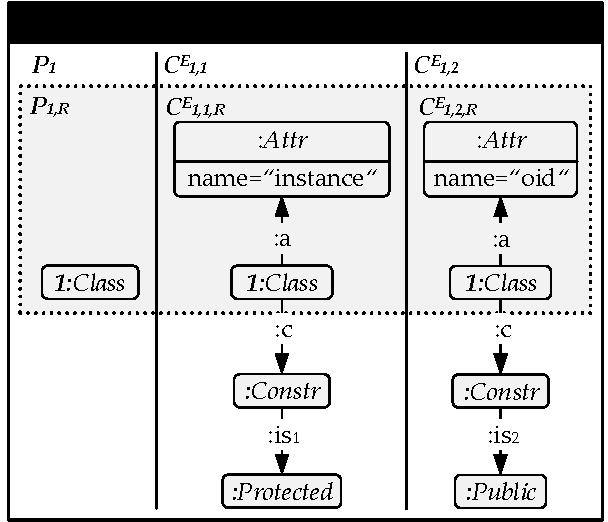
\includegraphics[width=.55\textwidth]{img/domain_res/res_ext.pdf}};
\fill (-1.25,3.15) node[inner sep=1pt] (B) {\textcolor{white}{$c_8=\vee_{i=(1,2)}(\exists(P_1 \to C^E_{1,i},\true))$}};
\end{tikzpicture}
\end{center}
\caption{Extended Domain Graph Constraint with Restriction}
\label{fig:sec-dc-general:res_ext}
\end{figure}

In \cref{sec-dom-compl-mt,thm:sec-dom-compl-mt:dom_compl_res_mt_II}, we instantiate the result from \cref{thm:sec-dc-general-res:dom_compl_res} to the domain completeness of model transformations under restrictions and show in \cref{sec-dom-compl-mt,fig:sec-dom-compl-mt:ex:dom_compl_1} that the transformation as defined by the $\TGG$ in \cref{fig:sec-dc-general:res_tg} is domain complete under restrictions if constraint $c_8$ from \cref{fig:sec-dc-general:res_ext} is added to the domain constraints in \cref{fig:sec-dc-general:res_c}.
This is necessary in order to obtain $C$-extension completeness for the example according to \cref{sec-dc-verification,def:C-extensionCompleteness}, i.e., to obtain extensions that can be created via the rules of the given $\TGG$.
Constraint $c_8$ is not contained in the initial set of domain constraints in \cref{fig:sec-dc-general:res_c}.
However, the constraint can be inferred from the initial set by performing $C$-extensions of the conclusion graphs of initial domain constraint $c_1$ via constraints $c_2$ and $c_3$ according to \cref{sec-dc-verification,def:C-extension}.
As in the example, the extension of domain constraints is useful for the verification of domain completeness under restrictions if the verification is based on the verification of domain completeness w.r.t. restricted domain constraints according to \cref{thm:sec-dc-general-res:dom_compl_res} and $C$-extension completeness cannot be successfully verified based on the initial set of restricted domain constraints but based on an extended set that additionally contains constraints that are inferred from initial constraints via elements outside the restriction, as it is the case for constraint $c_8$ where class constructors and their visibilities are taken into account for the inference but which are omitted in the restricted constraints.
Therefore, we propose to extend the initial set of domain constraints at first and then to use the refined set for verifying domain completeness under restrictions.
In \cref{def:sec-dc-general-res:ext_constr}, we define the step-wise extension of conditions and show in \cref{thm:sec-dc-general-res:ext_constr} that a graph satisfies the initial constraints if and only if it does also satisfy the extended constraints implying further that the language over the initial set of domain constraints equals to the language over the refined set.
Therefore, the refined set of constraints can be used instead of the initial set when verifying domain completeness.
Note that we restrict to extensions of plain conditions without multiple nestings.
However, we are confident that the approach can be extended to conditions with arbitrary nestings such that \cref{thm:sec-dc-general-res:ext_constr} holds, in future work.

\begin{definition}[$C$-Extensions of Conditions]
\label{def:sec-dc-general-res:ext_constr}
Let $\ac_P$ be a plain condition and $C$ be a set of conditions.
\emph{The extensions $Extensions(\ac_P,C)$ of $\ac_P$ via $C$}\index{graph condition!$C$-extensions} is inductively defined as follows based on the $C$-extensions of conclusion graphs according to \cref{sec-dc-verification,def:C-extension}:
$
  \begin{array}[t]{ll}
  Extensions(\ac_P,C) = \{\true\} & , \text{ for } \ac_P=\true, \\
  Extensions(\ac_P,C) = \{\vee_{i \in \{1,\ldots,n\}}(\exists(P \trans{e_i \circ a} E_i,\true)) \mid & , \text{ for } \ac_P=\exists(a\colon P \to C',\true),\\
  E=\{E_1,\ldots,E_n\} \in Extensions(C',C)\} \text{ where } e_i\colon C' \to E_i & \\
  \text{is the induced morphism according to \cref{sec-dc-verification,def:C-extension}} & \\
  Extensions(\ac_P,C) = \{\vee_{i \in I}(e_{P,i}) \mid e_{P,i} \in Extensions(\ac_{P,i},C)\} & , \text{ for } \ac_P=\vee_{i \in I}(\ac_{P,i}),\\
  Extensions(\ac_P,C) = \{\wedge_{i \in I}(e_{P,i}) \mid e_{P,i} \in Extensions(\ac_{P,i},C)\} & , \text{ for } \ac_P=\wedge_{i \in I}(\ac_{P,i}), and \\
  Extensions(\ac_P,C) = \{\neg e_P \mid e_P \in Extensions(\ac'_P,C)\} & , \text{ for } \ac_P=\neg\ac'_P.
  \end{array}
$
\envEndMarker
\end{definition}

\begin{example}[$C$-Extensions of Conditions]
The condition in \cref{fig:sec-dc-general:res_ext} is an extension of condition $c_1$ in \cref{fig:sec-dc-general:res_c} via conditions $c_2$ and $c_3$.
\envEndMarker
\end{example}

Note that in \cref{thm:sec-dc-general-res:ext_constr}, conditions are extended via conditions that are designated for general satisfaction only.
If we allow the extension of conditions via conditions that are designated for initial satisfaction, then \cref{thm:sec-dc-general-res:ext_constr} may not hold. 
For example, consider two constraints ``Each node \code{:A} is connected to two \code{:B} nodes'' and ``There exists a \code{:B} node connected to a \code{:C} node''.
The extension of the first constraint via the second constraint may lead to a constraint ``Each node \code{:A} is connected to two \code{:B} nodes and furthermore, each of the two \code{:B} nodes is connected to a \code{:C} node''.
Therefore, the existential characteristic of the \code{:B} node in the second constraint switches to a universal characteristic in the extended constraint.
Thus, a graph which satisfies the first initial constraint may not satisfy the extended constraint.

\begin{theorem}[Equivalence of Languages over Constraints \& Extended Constraints]
\label{thm:sec-dc-general-res:ext_constr}
In an $\M$-adhesive category with effective pushouts, let $C_I \cup C_G$ be a set of constraints where constraints $C_I$ are designated for initial satisfaction and constraints $C_G$ are designated for general satisfaction.
Furthermore, let $C'_I$ ($C'_G$) be a set of extensions of conditions $C_I$ ($C_G$) via $C_G$.
Then, it holds that $G \in \Lang_I(C_I) \cap \Lang(C_G)$ if and only if $G \in \Lang_I(C_I \cup C'_I) \cap \Lang(C_G \cup C'_G)$.
Therefore, $\Lang_I(C_I) \cap \Lang(C_G)=\Lang_I(C_I \cup C'_I) \cap \Lang(C_G \cup C'_G)$.
\envEndMarker
\end{theorem}

\begin{proof}
The proof is presented in \cref{sec-proofs:thm:sec-dc-general-res:ext_constr}.
\end{proof}


\chapter{Domain Completeness of Model Transformations \& Model Synchronisations}
\label{sec-dom-compl-mt-synch}

\section{Domain Completeness of Model Transformations}
\label{sec-dom-compl-mt}
Given a model transformation $\MT\colon \Lang(C^S) \TransMT \Lang(D_2)$ from source DSL $\Lang(C^S)$ that is restricted by source domain graph constraints $C^S$ to target DSL $\Lang(D_2)$ in target domain $D_2$, then $\MT$ is domain complete if each source model $G^S \in \Lang(C^S)$ can be completely translated via a model transformation sequence in the sense that all elements of the graph are translated exactly once by changing their translation attributes from $\False$ to $\True$.

\paragraph*{General Assumption:}
As with the results for verifying domain completeness in \cref{sec-dc-verification}, we assume that the results of this Chapter are applied in the context $(\ATrGraphs_\ATGI,\M)$ of typed, attributed triple graphs with node type inheritance and common triple type graph $\ATGI$.
This is due to the fact that the node and edge attributes are used as markings (translation attributes) for checking conflict-freeness of rules.
Moreover, translation attributes are used for an intuitive definition of domain completeness of model transformations in \cref{def:sec-dom-compl-met:dc}.
Note that according to \cref{sec-dc-general,def:sec-dc-general:lang}, we write $C$ short for a set of constraints $C=C_I \cup C_G$ that is composed of constraints $C_I$ that are designated for initial satisfaction and constraints $C_G$ that are designated for general satisfaction.
Analogously, we write $\Lang(C)$ short for $\Lang_I(C_I) \cap \Lang(C_G)$.
%If not made explicit, we assume that a given triple graph grammar $\TGG$ and domain constraints $C$ are typed over the same type graph.

\begin{definition}[Domain Completeness of Model Transformations]
\label{def:sec-dom-compl-met:dc}
Let $C^S$ be the set of source domain graph constraints and $\Lang(C^S)$ be the source domain-specific language of graphs. 
Furthermore, let $\TGG$ be a triple graph grammar that specifies the translation $\MT\colon \Lang(C^S) \TransMT \Lang(D_2)$ of graphs in $\Lang(C^S)$ into graphs in the target domain-specific language $\Lang(D_2)$.
%For typing, $C^S$ is typed over some type graph $\TG^S$ and $\TGG$ is typed over some triple type graph $(\TG^S \gets \TG^C \to \TG^T)$, i.e., both coincide on $\TG^S$.
\emph{The model transformation $\MT$ is domain complete}\index{model transformation!domain completeness}, if for each graph $G^S \in \Lang(C^S)$ there is a model transformation sequence $(G^S,G_0 \Trans{\tr^*_\FT} G_n,G^T)$ based on the forward translation rules of $\TGG$ with $G_0=(\Att^\False(G^S) \gets \varnothing \to \varnothing)$ and $G_n=(\Att^\True(G^S) \gets G^C \to G^T)$.
\envEndMarker
\end{definition}

Based on the ``classical" syntactical completeness and correctness of model transformations by TGGs based on forward translation rules (cf. \cref{sec-gen-intro-compl,rem:sec-gen-intro-compl:classical_corr_compl_mt}), the domain completeness of model transformations from \cref{def:sec-dom-compl-met:dc} can be redefined as follows.
While \cref{def:sec-dom-compl-met:dc} reflects the intuitive meaning behind complete transformations, \cref{fact:sec-dom-compl-mt:comp} expresses completeness in terms of a language inclusion which can be verified by using the verification techniques for domain completeness.
Therefore, both formulations of completeness in \cref{def:sec-dom-compl-met:dc,fact:sec-dom-compl-mt:comp} are equivalent.

\begin{theorem}[Domain Completeness of Model Transformations]
\label{fact:sec-dom-compl-mt:comp}
Let $\MT\colon \Lang(C^S) \TransMT \Lang(D_2)$ be a model transformation based on forward translation rules of a given $\TGG$.
Transformation $\MT$ is domain complete according to \cref{def:sec-dom-compl-met:dc} if and only if domain completeness w.r.t. $\Lang(C^S)$ and $\Lang(\TGG)^S$ holds in the sense of \cref{sec-dc-general,def:sec-dc-general:dcp}, i.e., $\Lang(C^S) \subseteq \Lang(\TGG)^S$.
\envEndMarker
\end{theorem}

\begin{proof}
\begin{enumerate}
  \item[\textbf{``$\Rightarrow$''}] For each $G^S \in \Lang(C^S)$ with corresponding model transformation sequence based on forward translation rules the ``classical" correctness implies that $G^S \in \Lang(\TGG)^S$ (cf. \cref{sec-gen-intro-compl,rem:sec-gen-intro-compl:classical_corr_compl_mt}).
  \item[\textbf{``$\Leftarrow$''}] By ``classical" completeness, for each $G^S \in \Lang(C^S) \cap \Lang(\TGG)^S$ there is a model transformation sequence $(G^S,G_0 \Trans{\tr^*_\FT} G_n,G^T)$ based on forward translation rules with $G_0=(\Att^\False(G^S) \gets \varnothing \to \varnothing)$ and $G_n=(\Att^\True(G^S) \gets G^C \to G^T)$ (cf. \cref{sec-gen-intro-compl,rem:sec-gen-intro-compl:classical_corr_compl_mt}).
\end{enumerate}
\end{proof}

%For TGGs without application conditions, 
Similarly to the verification of domain completeness for flat graphs in \cref{sec-dc-verification,thm:C-extensionCompleteness}, we verify the language inclusion $\Lang(C^S) \subseteq \Lang(\TGG)^S$ by verifying $C^S$-conflict-freeness from \cref{thm:C-extensionCompleteness} w.r.t. forward translation rules $\TR_\FT$, since, we only need to check for possible overlappings of extensions in the source domain.
Therefore, similarly to \cref{sec-dc-verification,def:cf-marking-rules}, we define the $C^S$-conflict-freeness of forward translation rules in \cref{def:sec-dom-compl-mt:cf-fwd}.
Note that in $C^S$-conflict-freeness of forward translation rules, only critical pairs need to be considered where the source component of the conflict triple graph $O$ occurs in graphs of $\Lang(C^S)$ (cf. \cref{def:sec-dom-compl-mt:cf-fwd,def:sec-dom-compl-mt:cf-fwd:1}) and conflict triple graph $O$ can be embedded in a triple graph $O'$ that can be created by a forward translation sequence (cf. \cref{def:sec-dom-compl-mt:cf-fwd,def:sec-dom-compl-mt:cf-fwd:2}).

\begin{definition}[$C^S$-Conflict-Freeness of Forward Translation Rules]
\label{def:sec-dom-compl-mt:cf-fwd}
Let $C^S$ be the source domain constraints and $\TR_\FT$ be the forward translation rules of triple rules $\TR$.
Then, \emph{$\TR_\FT$ is $C^S$-conflict-free}\index{triple rule!forward translation rule!$C$-conflict-freeness}, if for each critical pair $(K_1 \TransB{(\tr_{\FT,1},o_1)}\nobreak O=(O^S \gets O^C \to O^T) \Trans{(\tr_{\FT,2},o_2)} K_2)$ with $\tr_{\FT,1},\tr_{\FT,2} \in \TR_\FT$ where 
\begin{enumerate}
  \item \label{def:sec-dom-compl-mt:cf-fwd:1}$O^S$ is significant w.r.t. $\Lang(C^S)$ (or not $C^S$-inconsistent), and
  \item \label{def:sec-dom-compl-mt:cf-fwd:2}there is $O \to O' \in \M$ and forward translation sequence $(\Att^\False(\ol{O}) \gets \varnothing \to \varnothing) \Trans{\tr_\FT^*} O'$ via $\TR_\FT$,
\end{enumerate}
it is true that the rules and matches are the same ($\tr_{\FT,1}=\tr_{\FT,2},o_1=o_2$) (or it is true that the critical pair is strictly confluent).
\envEndMarker
\end{definition}

\begin{theorem}[Domain Completeness of Model Transformations]
% without Application Conditions]
\label{thm:sec-dom-compl-mt-without-acs}
Let $C^S$ be the source domain constraints in $\M$-normal form, $\Lang(C^S)$ be the source domain-specific language over $C^S$ and $\Lang(\TGG)$ be the language over a non-deleting triple graph grammar $\TGG=(\varnothing,\TR)$ with empty triple start graph $\varnothing$, all triple productions $\TR$ being non-trivial and where all application conditions are in $\M$-normal form.
Let $\TR_\FT$ be the derived set of forward translation rules from $\TGG$.
Furthermore, let $\MT$ be a model transformation based on forward translation rules $\TR_\FT$.
If the rules $\TR_\FT$ are $C^S$-conflict-free and $\Lang(\TGG')^S$ is $C^S$-extension complete where $\TGG'=(\varnothing',\TR)$ with $\varnothing'$ being the empty triple start graph with $\DSIG$-term algebra $T_\DSIG(X)$, then domain completeness w.r.t. $\Lang(C^S)$ and $\Lang(\TGG)^S$ holds for almost injective matches, i.e., it holds that $\Lang(C^S) \subseteq \Lang(\TGG)^S$.
\envEndMarker
\end{theorem}

\begin{proof}
The proof is basically identical to the proof of \cref{thm:C-extensionCompleteness}.
Let $G \in \Lang(C^S)$, $i\colon G_A \to G$ be an instance morphism and $A=(a_i)_{i \in \{1,\ldots,n\}} \in Atoms(G_A)$ be the atoms of $G_A$.
Analogously to \cref{thm:C-extensionCompleteness}, by $\forall a \in A.a \in EAtoms(C^S)$ and $\Lang(\TGG')^S$ is $C^S$-extension complete it follows that $\forall a \in A.\exists S_a \in Extensions(a,C^S_G)$ such that $S_a \subseteq \Lang(\TGG')^S$ by \cref{def:C-extensionCompleteness}.
Thus, $\forall a \in A.\exists S_a \in Extensions(a,C^S_G)$ such that $\forall s \in S_a.\exists$ triple graph $(s \gets s^C \to s^T) \in \Lang(\TGG')$ and model transformation sequence $(s,(\Att^\False(s) \gets \varnothing \to \varnothing) \Trans{\tr_\FT^*} (\Att^\True(s) \gets s^C \to s^T),s^T)$ based on forward translation rules $\TR_\FT$ by model transformation $\MT$ and \cref{sec-gen-intro-compl,rem:sec-gen-intro-compl:classical_corr_compl_mt}.
Note that for each such model transformation sequence and a given injective embedding $f\colon s \to s' \in \M$ there is a forward translation sequence $(\Att^\False(s') \gets \varnothing \to \varnothing) \Trans{\tr_\FT^*} (s' \oplus \Att^\True_{s} \oplus \Att^\False_{s' \setminus s} \gets s^C \to s^T)$ via forward translation rules $\TR_\FT$ analogously to \cref{sec-dc-verification,lem:equivalence-marking-emptySG} $^{(*^A)}$, since, all relevant elements of application conditions in rules $\TR_\FT$ are marked with $\True$ whereas the marking of all elements in $s' \setminus s$ remain $\False$ for the translation sequence and therefore, cannot be matched by the application conditions.
Analogously to the proof of \cref{thm:C-extensionCompleteness}, there is a function $f_{a_E}$ with $f_{a_E}(a)=s \in S_a,\forall a \in A=(a_i)_{i \in \{1,\ldots,n\}}$ such that there exist graphs $(G^E_j)_{1 \leq j \leq n-1}$ and pushouts $(PO^E_k +_{G^E_k} f_{a_E}(a_{k+1})=PO^E_{k+1})_{k \in \{1,\ldots,n-1\}}$ with pushout objects $PO^E_{k+1}$, $PO^E_1=f_{a_E}(a_1)$ and injective embeddings $i_{k,1}\colon PO^E_k \to PO^E_{k+1}$ and $i_{k,2}\colon f_{a_E}(a_{k+1}) \to PO^E_{k+1} \in \M$ where $PO^E_n=G_A$ by \cref{sec-dc-verification,lem:union-ext-atoms}.
For pushout $k=1$ we conclude as follows.
By $(*^A)$, there exists forward translation sequences $t_1\colon (\Att^\False(PO^E_2) \gets \varnothing \to \varnothing) \Trans{\tr_\FT^*} (PO^E_2 \oplus \Att^\True_{f_{a_E}(a_1)} \oplus \Att^\False_{PO^E_2 \setminus f_{a_E}(a_1)} \gets f_{a_E}(a_1)^C \to f_{a_E}(a_1)^T)$ and $t_2\colon (\Att^\False(PO^E_2) \gets \varnothing \to \varnothing) \Trans{\tr_\FT^*} (PO^E_2 \oplus \Att^\True_{f_{a_E}(a_2)} \oplus \Att^\False_{PO^E_2 \setminus f_{a_E}(a_2)} \gets f_{a_E}(a_2)^C \to f_{a_E}(a_2)^T)$ via forward translation rules $\TR_\FT$.
Analogously to the proof of \cref{thm:C-extensionCompleteness}, assumption $\TR_\FT$ is $C^S$-conflict-free implies that transformation system $\TR_\FT$ is confluent and therefore, there is a complete forward translation sequence $(\Att^\False(PO^E_2) \gets \varnothing \to \varnothing) \Trans{\tr_\FT^*} (\Att^\True(PO^E_2) \gets C_2 \to T_2)$, i.e., a model transformation sequence $(PO^E_2,(\Att^\False(PO^E_2) \gets \varnothing \to \varnothing) \Trans{\tr_\FT^*} (\Att^\True(PO^E_2) \gets C_2 \to T_2),T_2)$ based on forward translation rules $\TR_\FT$ for pushout object $PO^E_2$.
Note that the restriction to a subset of all critical pairs in $C^S$-conflict-freeness matches the situation, since, $G^A \in \Lang(C^S)$ and $\M$-composition of embeddings $i_{k,1},i_{k,2}$ imply that the source component of all conflict triple graphs of conflicts that may occur is significant w.r.t. $\Lang(C^S)$ (cf. \cref{def:sec-dom-compl-mt:cf-fwd,def:sec-dom-compl-mt:cf-fwd:1}) and furthermore, all such conflict triple graphs of conflicts that may occur are embedded in triple graphs that are created by forward translation sequences $t_1$ and $t_2$ (cf. \cref{def:sec-dom-compl-mt:cf-fwd,def:sec-dom-compl-mt:cf-fwd:2}).
Analogously, we iterate over all pushouts for $k=(1,\ldots,n-1)$ and obtain a model transformation sequence $(PO^E_n,(\Att^\False(PO^E_n) \gets \varnothing \to \varnothing) \Trans{\tr_\FT^*} (\Att^\True(PO^E_n) \gets C_n \to T_n),T_n)$ based on forward translation rules $\TR_\FT$ and almost injective matches.
By \cref{sec-gen-intro-compl,rem:sec-gen-intro-compl:classical_corr_compl_mt}, $PO^E_n=G_A \in \Lang(\TGG')^S$, i.e., there is $\varnothing' \Trans{*} (G_A \gets C_A \to T_A)$ via $\TR$.
We extend instance morphism $i\colon G_A \to G$ to a triple graph morphism $i'\colon (G_A \gets C_A \to T_A) \to (G \gets C \to T)$ that is an instance morphism componentwise for source, correspondence and target.
Analogously to the proof of \cref{thm:C-extensionCompleteness} by \cref{lem:atiti} componentwise with instance morphism $i'$ and all application conditions in $\TR$ being in $\M$-normal form there is a transformation $\varnothing \Trans{*} (G \gets C \to T)$ via $\TR$ and almost injective matches, i.e., $G \in \Lang(\TGG)^S$.
Therefore, $\Lang(C^S) \subseteq \Lang(\TGG)^S$.
\end{proof}

% For TGGs with application conditions, we additinal have to check for conflicts with application conditions in the target domain.
% Therefore, we use consistency creating rules instead of forward translation rules and omit critical pairs that overlap in the correspondence or target part.
% 
% \begin{definition}[C-conflict-freeness of Consistency Creating Rules]
% \label{def:cf-marking-rules}
% Let $C^S$ be a set of source domain constraints and let $\TR_\CC$ be the set of consistency creating rules as derived from a given $\TGG$.
% Then, \emph{$\TR_\CC$ is $C^S$-conflict-free}\index{consistency creating rule!C-conflict-freeness}, if for each critical pair $K_1 \TransB{p_1,o_1}\nobreak O \Trans{p_2,o_2} K_2$ that does not overlap in the correspondence and target part and is not $C^S$-inconsistent with $p_1,p_2 \in \TR_\CC$ it is true that the rules and matches are the same ($p_1=p_2,o_1=o_2$).
% \envEndMarker
% \end{definition}
% 
% \begin{theorem}[Domain Completeness of Model Transformations with Application Conditions]
% \label{thm:sec-dom-compl-mt-with-acs}
% Let $C^S$ be the source domain constraints, $\Lang(C^S)$ be the source domain language and $\Lang(\TGG)$ be the language over a non-deleting $\TGG$ with empty start triple graph.
% Let $\TR_\CC$ be the derived set of consistency creating rules from $\TGG$.
% If the rules $\TR_\CC$ are $C^S$-conflict-free and $\Lang(\TGG)^S$ is $C^S$-extension complete, then domain completeness w.r.t. $\Lang(C^S)$ and $\Lang(\TGG)^S$ holds, i.e., $\Lang(C^S) \subseteq \Lang(\TGG)^S$.
% \envEndMarker
% \end{theorem}
% 
% \nn{
% \begin{proof}
% 
% \end{proof}
% }

According to domain completeness under restrictions in \cref{sec-dc-general-res}, we define domain completeness of model transformations under restrictions.
This is important for model transformations that only cover specific elements of each graph in the source DSL.
For example, the model transformation in \cref{sec-dc-general-res} from class diagrams (CDs) to relational database models (RDBMs) only covers the elements of the restricted type graph $\TG_{\CD,R}$ in \cref{fig:sec-dc-general:res_tg}, i.e., classes and their attributes in class diagrams, while neglecting class constructors and their visibilities.
In contrast to ``full'' domain completeness of the transformation which requires that all class diagrams can be completely translated into RDBMs, domain completeness under restrictions only requires that all classes and their attributes in each class diagram can be completely translated into corresponding tables and columns.

\begin{definition}[Domain Completeness of Model Transformations under Restrictions]
\label{def:sec-dom-compl-mt:dom_compl_res_mt}
Let $t\colon \TG^S_R \to \TG^S \in \M$ be a type morphism and $\TG^S_R$ be the restriction of source type graph $\TG^S$.
Let $\TG=(\TG^S_R \gets \TG^C \to \TG^T)$ be a triple type graph.
Let $C^S$ be the set of source domain graph constraints typed over $\TG^S$ and $\Lang(C^S)$ be the source domain-specific language of graphs. 
Furthermore, let $\TGG$ be a triple graph grammar typed over $\TG$ that specifies the translation $\MT\colon \Lang(C^S) \TransMT \Lang(D_2)$ of graphs in $\Lang(C^S)$ into graphs in the target domain-specific language $\Lang(D_2)$.
\emph{The model transformation $\MT$ is domain complete under restrictions}\index{model transformation!domain completeness!under restrictions}, if for the restriction $\Restr_t(G^S)$ of each graph $G^S \in \Lang(C^S)$ along $t$ there is a model transformation sequence $(\Restr_t(G^S),G_0 \Trans{\tr^*_\FT} G_n,G^T)$ based on the forward translation rules of $\TGG$ with $G_0=(\Att^\False(\Restr_t(G^S)) \gets \varnothing \to \varnothing)$ and $G_n=(\Att^\True(\Restr_t(G^S)) \gets G^C \to G^T)$.
\envEndMarker
\end{definition}

Similarly to \cref{fact:sec-dom-compl-mt:comp}, in \cref{thm:sec-dom-compl-mt:dom_compl_res_mt_I} we reformulate domain completeness of model transformations under restrictions by domain completeness under restrictions in the sense of \cref{def:sec-dc-general-res:dc_prob} which can be verified by verifying domain completeness w.r.t. restricted constraints as stated in \cref{thm:sec-dom-compl-mt:dom_compl_res_mt_II}.
In turn, domain completeness can be verified based on \cref{thm:sec-dom-compl-mt-without-acs}.

\begin{theorem}[Domain Completeness of Model Transformations under Restrictions]
\label{thm:sec-dom-compl-mt:dom_compl_res_mt_I}
Let $\MT\colon \Lang(C^S) \TransMT \Lang(D_2)$ be a model transformation based on forward translation rules of a given $\TGG$.
Transformation $\MT$ is domain complete under restrictions according to \cref{def:sec-dom-compl-mt:dom_compl_res_mt} if and only if domain completeness under restrictions w.r.t. $\Lang(C^S)$ and $\Lang(\TGG)^S$ holds in the sense of \cref{def:sec-dc-general-res:dc_prob}.
\envEndMarker
\end{theorem}

\begin{proof}
Let $G^S \in \Lang(C^S)$ and $\Restr_t(G^S)$ be its restriction along $t$.
\begin{enumerate}
  \item [``$\Rightarrow$''] By assumption, there is a model transformation sequence $(\Restr_t(G^S),G_0 \Trans{\tr^*_\FT} G_n,G^T)$ based on forward translation rules.
  By ``classical" syntactical correctness of model transformations based on foward translation rules, $\Restr_t(G^S) \in \Lang(\TGG)^S$.
  \item [``$\Leftarrow$''] By assumption, $\Restr_t(G^S) \in \Lang(\TGG)^S$.
  By ``classical'' syntactical completeness of model transformations based on forward translation rules, there is a model transformation sequence $(\Restr_t(G^S),G_0 \Trans{\tr^*_\FT} G_n,G^T)$ based on forward translation rules.
\end{enumerate}
\end{proof}

\begin{corollary}[Domain Completeness of Model Transformations under Restrictions]
\label{thm:sec-dom-compl-mt:dom_compl_res_mt_II}
In the context of \cref{thm:sec-dom-compl-mt:dom_compl_res_mt_I}, domain completeness under restrictions w.r.t. $\Lang(C^S)$ and $\Lang(\TGG)^S$ holds if according to \cref{thm:sec-dc-general-res:dom_compl_res} domain completeness w.r.t. $\Lang_I(\Restr_t(C^S_I)) \cap \Lang(\Restr_t(C^S_G))$, $\Lang(\TGG)^S$ and $\TG^S_R$ holds with $C^S=C^S_I \cup C^S_G$.
\envEndMarker
\end{corollary}

\begin{proof}
This follows directly by \cref{thm:sec-dc-general-res:dom_compl_res,thm:sec-dc-general-res:dom_compl_res:item2,thm:sec-dc-general-res:dom_compl_res:item1}.
\end{proof}

Based on the reformulations of domain completeness of model transformations (under restrictions) in \cref{fact:sec-dom-compl-mt:comp,thm:sec-dom-compl-mt:dom_compl_res_mt_I} and the result from \cref{thm:sec-dom-compl-mt:dom_compl_res_mt_II}, the following relationship between the notions of domain completeness and domain completeness under restrictions does exist.

\begin{corollary}[Relationship between Domain Completeness of Model Transformations \& Domain Completeness under Restrictions]
\label{thm:sec-dom-compl-mt:dom_compl_res_mt_equiv}
Let $\MT\colon \Lang(C) \TransMT \Lang(D_2)$ and $\MT_R\colon \Lang(\Restr_t(C)) \TransMT \Lang(D_2)$ be two model transformations defined by the same $\TGG$ where according to \cref{thm:sec-dc-general-res:dom_compl_res}, $\Lang(\Restr_t(C))=\Lang_I(\Restr_t(C_I)) \cap \Lang(\Restr_t(C_G))$ for $C=C_I \cup C_G$.
If $\MT_R$ is domain complete according to \cref{def:sec-dom-compl-met:dc}, then $\MT$ is domain complete under restrictions according to \cref{def:sec-dom-compl-mt:dom_compl_res_mt}.
\envEndMarker
\end{corollary}

\begin{proof}
By \cref{fact:sec-dom-compl-mt:comp}, domain completeness of $\MT_R$ implies domain completeness w.r.t. $\Lang(\Restr_t(C))$, $\Lang(\TGG)^S$ and $\TG^S_R$.
By \cref{thm:sec-dom-compl-mt:dom_compl_res_mt_II}, it follows domain completeness under restrictions w.r.t. $\Lang(C)$ and $\Lang(\TGG)^S$ implying further that $\MT$ is domain complete under restrictions by \cref{thm:sec-dom-compl-mt:dom_compl_res_mt_I}.
\end{proof}

\begin{figure}[!tb]
\begin{center}
\begin{tikzpicture}[]
\fill (0,0) node[inner sep=1pt] (A) {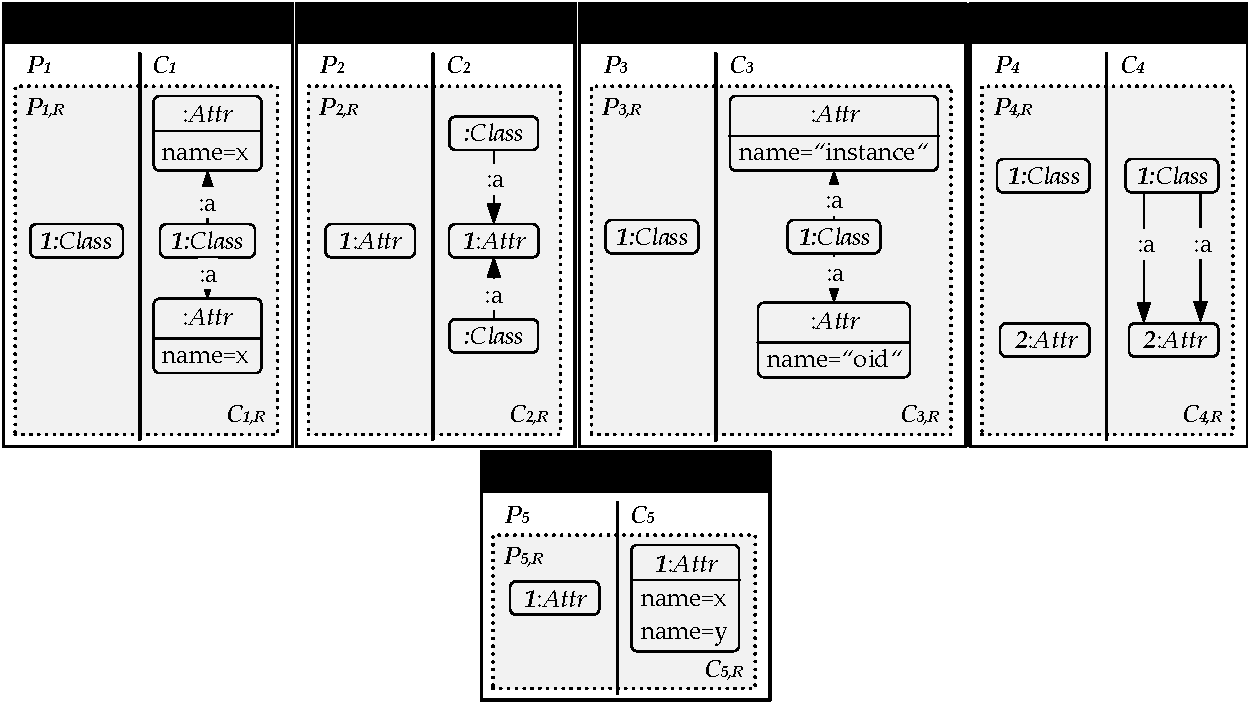
\includegraphics[width=\textwidth]{img/domain_mt/constraints.pdf}};
\fill (-5.65,3.85) node[inner sep=1pt] (B) {\footnotesize{\textcolor{white}{$c_9=\neg\exists(P_1 \to C_1,\true)$}}};
\fill (-2.2,3.85) node[inner sep=1pt] (C) {\footnotesize{\textcolor{white}{$c_{10}=\neg\exists(P_2 \to C_2,\true)$}}};
\fill (1.2,3.85) node[inner sep=1pt] (D) {\footnotesize{\textcolor{white}{$c_{11}=\neg\exists(P_3 \to C_3,\true)$}}};
\fill (5.75,3.85) node[inner sep=1pt] (E) {\footnotesize{\textcolor{white}{$c_{12}=\neg\exists(P_4 \to C_4,\true)$}}};
\fill (0,-1.45) node[inner sep=1pt] (F) {\footnotesize{\textcolor{white}{$c_{13}=\neg\exists(P_5 \to C_5,\true)$}}};
\end{tikzpicture}
\end{center}
\caption{Additional Domain Graph Constraints with Restrictions}
\label{fig:sec-dom-compl-mt:constraints}
\end{figure}

\begin{figure}[!tb]
\begin{center}
\begin{tikzpicture}[]
\fill (0,0) node[inner sep=1pt] (A) {\includegraphics[width=.5\textwidth]{img/domain_mt/agg.png}};
\fill (-7.5,0) node[inner sep=1pt] (B) {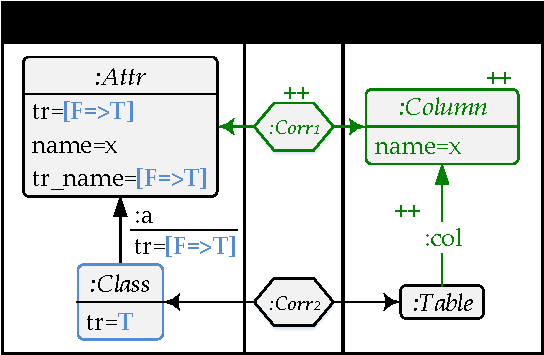
\includegraphics[width=.45\textwidth]{img/domain_mt/ft.pdf}};
\fill (-9.3,1.9) node[inner sep=1pt] (C) {\textcolor{white}{Attr2Column-FT}};
\end{tikzpicture}
\end{center}
\caption{Foward Translation Rule \code{Attr2Column-FT} (left) \& Conflict Analysis of Forward Translation Rules with AGG (right)}
\label{fig:sec-dom-compl-mt:agg}
\end{figure}

\begin{figure}[!tb]
\begin{center}
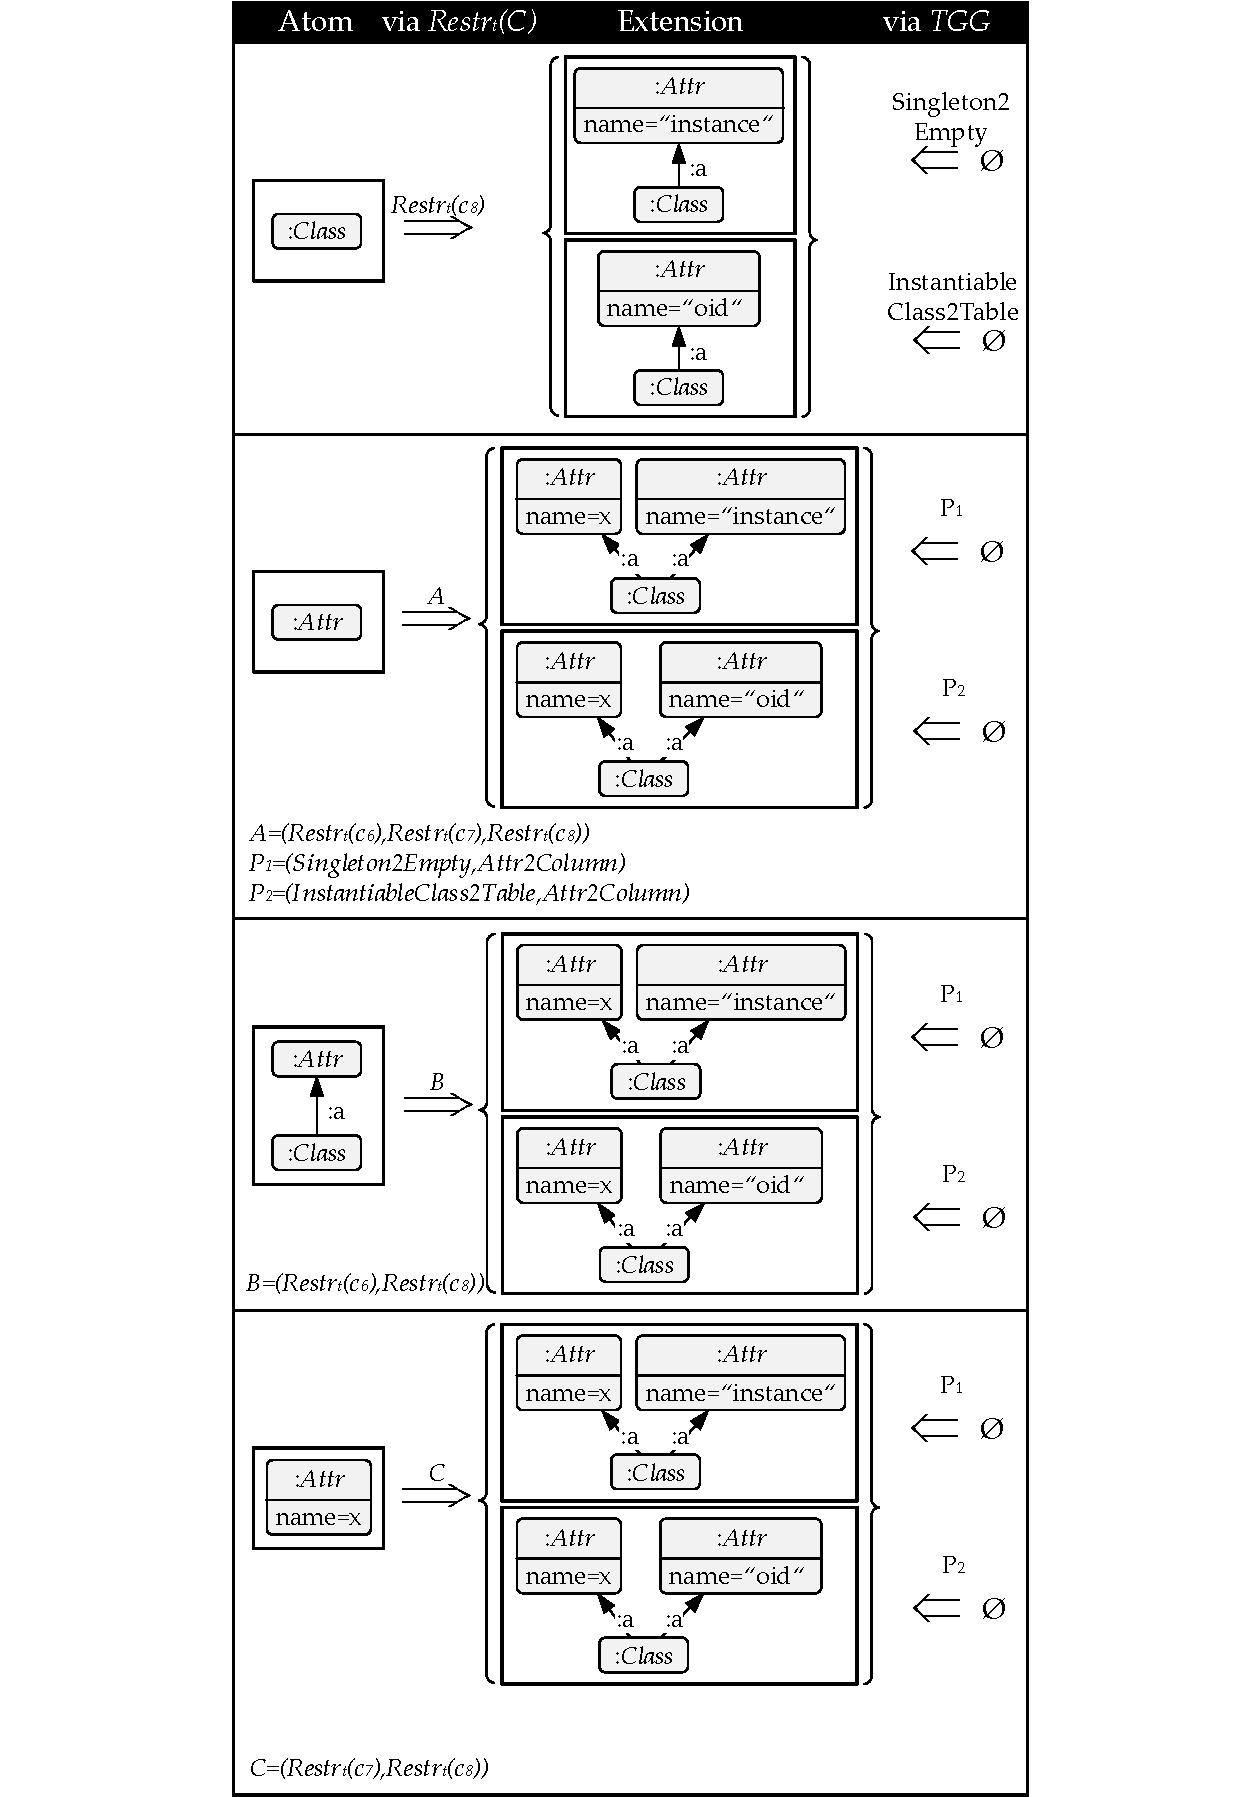
\includegraphics[width=\textwidth]{img/domain_mt/ext.pdf}
\end{center}
\caption{Verification of $\Restr_t(C)$-Extension Completeness of $\Lang(\TGG)^S$}
\label{fig:sec-dom-compl-mt:ext}
\end{figure}

\begin{example}[Domain Completeness of Model Transformations under Restrictions]
\label{fig:sec-dom-compl-mt:ex:dom_compl_1}
The model transformation $\MT\colon \Lang(C) \TransMT \Lang(\TG_\RDBM)$ from UML class diagrams (CDs) to relational database models (RDBMs) as defined by the $\TGG$ with empty start graph and triple rules without application conditions and typed over $\TG_{\CD,R}$ from \cref{sec-dc-general-res,fig:sec-dc-general:res_tg} is not domain complete w.r.t. the domain constraints $C=\{c_1,\ldots,c_{13}\}$ in \cref{fig:sec-dc-general:res_c,fig:sec-dc-general:res_ext,fig:sec-dom-compl-mt:constraints}, since, class constructors together with their visibilities are not covered by the given $\TGG$.
We assume that all constraints $c \in C$ are designated for general satisfaction, i.e., $C=C_I \cup C_G$ with $C_I=\varnothing$ and $C_G=C$.
However, the model transformation is domain complete under restrictions w.r.t. domain constraints $C$, the given $\TGG$, type morphism $t\colon \TG_{\CD,R} \to \TG_\CD \in \M$ and restriction $\TG_{\CD,R}$.
Thus, all \code{Class}es and \code{Attr}ibutes in each CD can be translated to corresponding \code{Table}s and \code{Column}s in RDBMs.
In order to show this, by \cref{thm:sec-dom-compl-mt:dom_compl_res_mt_II}, we have to verify domain completeness w.r.t. the restricted domain constraints $\Restr_t(C)$, the given $\TGG$ and restricted type graph $\TG_{\CD,R}$, i.e., by \cref{fact:sec-dom-compl-mt:comp} domain completeness of model transformation $\MT_R\colon \Lang(\Restr_t(C)) \TransMT \Lang(\TG_\RDBM)$ from class diagrams that are typed over $\TG_{\CD,R}$ and satisfy the restricted constraints $\Restr_t(C)$ to RDBMs that are typed over $\TG_\RDBM$.
By \cref{thm:sec-dom-compl-mt-without-acs}, we have to check that the forward translation rules of $\TGG$ are $\Restr_t(C)$-conflict-free and furthermore, $\Lang(\TGG)^S$ is $\Restr_t(C)$-extension complete.
According to \cref{sec-dc-general-res,thm:sec-dc-general-res:dom_compl_res}, $\Restr_t(C)=\{\Restr_t(c_1),\Restr_t(c_6),\Restr_t(c_7),\Restr_t(c_8),\Restr_t(c_9),\Restr_t(c_{10}),\Restr_t(c_{11}),\Restr_t(c_{12}),$ $\Restr_t(c_{13})\}$ while constraints $c_2$ to $c_5$ are neglected for the verification, as, they are positive but 
%not restricted 
unrestricted along $t$ ($c_2$ to $c_4$) or negative but not purely restricted along $t$ ($c_5$).
The restricted constraints are highlighted by grey boxes in \cref{fig:sec-dc-general:res_c,fig:sec-dc-general:res_ext,fig:sec-dom-compl-mt:constraints} with premises $P_{\_,R}$ and conclusions $C^{[E]}_{\_,R}$.
\cref{fig:sec-dom-compl-mt:agg} (left) shows the forward translation rule \code{Attr2Column-FT} of triple rule \code{Attr2Column} in \cref{fig:sec-dc-general:res_tg}.
Analogously, we derive forward translation rules \code{InstantiableClass2Table-FT} and \code{Singleton2Empty-FT} for triple rules \code{InstantiableClass2Table} and \code{Singleton2Empty}.
\cref{fig:sec-dom-compl-mt:agg} (right) depicts the result of the conflict analysis of the forward translation rules with AGG \cite{AGG} while omitting conflicts of the same rule and same match.
Altogether, there are eight conflicts that are reflected by constraints $c_9$ to $c_{12}$ in \cref{fig:sec-dom-compl-mt:constraints}, i.e., each conclusion represents a conflict graph where the conflict occurs in the premise part of the conclusion, respectively.
Note that the conflicts are actually caused by updates of translation attributes but the translation attributes are not depicted explicitly in \cref{fig:sec-dom-compl-mt:constraints}.
In more detail, between rule \code{InstantiableClass2Table-FT} itself and \code{Singleton2Empty-FT} itself there are three conflicts, respectively, as reflected by conclusions $C_1,C_2$ and $C_4$.
This is due to the fact that both rules may translate
\begin{enumerate*}
\item the same \code{Class} but not the same \code{Attr}ibute, or
\item the same attribute but not the same class, or
\item the same class and attribute but not the same edge \code{:a} the assigns the attribute to the class.
\end{enumerate*}
Therefore, we forbid the following obvious patterns in class diagrams by constraints $c_9,c_{10}$ and $c_{12}$:
\begin{enumerate*}
  \item Constraint $c_9$ claims that each class does not have two or more attributes of the same name.
  \item Constraint $c_{10}$ claims that each attribute is assigned to at most one class.
  \item Constraint $c_{12}$ claims that for each two classes and attributes there is at most one assignment edge \code{:a} between both.
\end{enumerate*}
Between rules \code{InstantiableClass2Table-FT} and \code{Singleton2Empty-FT} and vice versa there is one conflict, respectively, as reflected by conclusion $C_3$.
This is due to the fact that both rules may translate the same class while translating different attributes \code{``instance''} and \code{``oid''} of that class.
Therefore, we forbid the pattern of a class that has attributes \code{``instance''} and \code{``oid''} at the same time in class diagrams by constraint $c_{11}$, i.e., class diagrams are not allowed to contain classes that are both instantiable and singleton at the same time.
Thus, by adding constraints $c_9$ to $c_{12}$ to domain constraints $c_1$ to $c_8$, the forward translation rules are $\Restr_t(C)$-conflict-free.
It remains to verify that $\Lang(\TGG)^S$ is $\Restr_t(C)$-extension complete.
The successful verification is depicted in \cref{fig:sec-dom-compl-mt:ext}.
Each atom over restricted type graph $\TG_{\CD,R}$ can be extended via restricted constraints $\Restr_t(C)$ such that the extension can be created by applying the triple rules of the given $\TGG$ with starting at the empty start graph $\varnothing$:
\begin{enumerate}
  \item \label{fig:sec-dom-compl-mt:ex:item1} The atom with a single \code{:Class} node can be extended via $\Restr_t(c_8)$ to two graphs, i.e., one graph with additional \code{``instance''} attribute and one with additional \code{``oid''} attribute, and both graphs can be created via rule \code{Singleton2Empty} or \code{InstantiableClass2Table}, respectively.
  \item \label{fig:sec-dom-compl-mt:ex:item2} The atom with a single \code{:Attr}ibute node can be extended via restricted constraints $\Restr_t(c_6),\Restr_t(c_7)$ and $\Restr_t(c_8)$ successively to two graphs, i.e., one graph with two additional \code{``instance''} and \code{x} attributes and one with two additional \code{``oid''} and \code{x} attributes, and both graphs can be created via rules \code{Singleton2Empty} and \code{Attr2Column} OR \code{InstantiableClass2Table} and \code{Attr2Column} successively.
  \item \label{fig:sec-dom-compl-mt:ex:item3} The atom with an \code{:Attr}ibute node, \code{:Class} node and \code{:a}ssignment edge in between can be extended via $\Restr_t(c_6)$ and $\Restr_t(c_8)$ successively to the same two graphs as in \cref{fig:sec-dom-compl-mt:ex:item2}.
  \item \label{fig:sec-dom-compl-mt:ex:item4} The same is true for the atom with a single \code{:Attr}ibute node and node attribute \code{name} via $\Restr_t(c_7)$ and $\Restr_t(c_8)$ successively.
  Note that constraint $c_{13}$ is essential for building the extensions, e.g., the second extension step in \cref{fig:sec-dom-compl-mt:ex:item4} via $\Restr_t(c_8)$ may also lead to an overlapping resulting in an extension graph $G_E$ where node \code{:Attr} has two \code{name} attributes which cannot be created via the rules of the $\TGG$.
  However, due to constraint $c_{13}$, graph $G_E$ does not occur in extensions, since, $G_E$ is $\Restr_t(C)$-inconsistent according to \cref{def:C-extension}.
\end{enumerate}
Therefore, the model transformation $\MT_R$ from class diagrams typed over $\TG_{\CD,R}$ that satisfy the restricted domain constraints $\Restr_t(C)$ to RDBMs is domain complete implying further according to \cref{thm:sec-dom-compl-mt:dom_compl_res_mt_equiv} that the model transformation $\MT$ from class diagrams typed over $\TG_\CD$ that satisfy the original domain constraints $C$ to RDBMs is domain complete under restrictions w.r.t. the given $\TGG$, type morphism $t$ and restricted type graph $\TG_{\CD,R}$.
\envEndMarker
\end{example}

\begin{figure}[!tb]
\begin{center}
\begin{tikzpicture}[]
\fill (0,0) node[inner sep=1pt] (A) {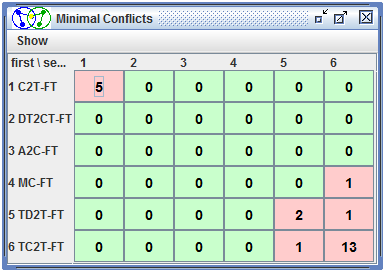
\includegraphics[width=.55\textwidth]{img/domain_mt/agg2.png}};
\fill (-7.75,0) node[inner sep=1pt] (B) {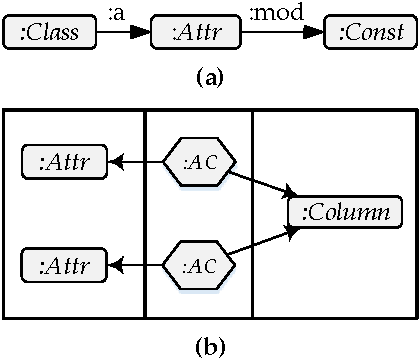
\includegraphics[width=.4\textwidth]{img/domain_mt/pattern.pdf}};
\end{tikzpicture}
\end{center}
\caption{Graph Pattern of Conflict Graphs (a) and (b) \& Conflict Analysis of Forward Translation Rules with AGG (right)}
\label{fig:sec-dom-compl-mt:agg2}
\end{figure}

\begin{example}[Domain Completeness of Model Transformations with Application Conditions]
\label{ex:sec-dom-compl-mt:domcp}
Given the model transformation CD2RDBM from UML class diagrams to relational database models in \cref{sec-mt-tgg,ex:sec-mt-tgg:fwd_mt} based on the forward translation rules $\TR_\FT$ of the triple rules $\TR$ with application conditions in \cref{sec-gt-trafo,fig:sec-gt-trafo:tgg} with triple graph grammar $CD2RDBM=(\varnothing,\TR)$ in \cref{sec-tgg,ex:sec-tgg:tg} that is typed over triple type graph $\TG=(\TG_\CD \gets \TG_C \to \TG_\RDBM)$ in \cref{sec-gt-graphs,fig:sec-gt-graphs:atg}.
Furthermore, given the source domain constraints $C^S$ for UML class diagrams in \cref{sec-gt-gc,ex:sec-gc-gc:gc_UML_CD} that are typed over type graph $\TG_\CD$.
\cref{fig:sec-dom-compl-mt:agg2} (right) depicts the result of the conflict analysis of forward translation rules $\TR_\FT$ via AGG \cite{AGG} where all critical pairs that are directly strict confluent and all critical pairs with conflict graphs that do not satisfy the multiplicity constraints in $\TG_\CD$ in the source component, respectively, are already omitted.
Note that critical pairs with conflict graphs whose source component violates a negative constraint in $C^S$ is $C^S$-inconsistent according to \cref{def:sec-dom-compl-mt:cf-fwd,def:sec-dom-compl-mt:cf-fwd:1} and therefore also not significant w.r.t. $\Lang(C^S)$ by \cref{sec-dc-verification,rem:sec-gc-verification} and thus, can be omitted by \cref{def:sec-dom-compl-mt:cf-fwd,def:sec-dom-compl-mt:cf-fwd:1}.
In total there are the following 23 critical pairs remaining:
\begin{enumerate}
  \item For forward translation rule \code{C2T-FT}, the source component of the conflict graph $O$ of each of the five critical pairs contains two \code{Classes} having the same \code{name} which is forbidden by constraint \code{12}.
  Therefore, the five critical pairs can be omitted by \cref{def:sec-dom-compl-mt:cf-fwd,def:sec-dom-compl-mt:cf-fwd:1}.
  \item For the critical pair of rules \code{MC-FT} and \code{TC2T-FT}, the source component of the conflict graph contains graph pattern \cref{fig:sec-dom-compl-mt:agg2} (a) which is forbidden by constraints \code{9} and \code{15}.
  Therefore, this critical pair can be omitted by \cref{def:sec-dom-compl-mt:cf-fwd,def:sec-dom-compl-mt:cf-fwd:1}.
  \item The conflict graphs of the remaining critical pairs contain triple graph pattern \cref{fig:sec-dom-compl-mt:agg2} (b), respectively, which cannot be created by forward translation sequences via $\TR_\FT$.
  Thus, these critical pairs can also be omitted by \cref{def:sec-dom-compl-mt:cf-fwd,def:sec-dom-compl-mt:cf-fwd:2}.
\end{enumerate}
Therefore, the forward translation rules $\TR_\FT$ are $C^S$-conflict-free.
$C^S$-extension completeness of $\Lang(CD2RDBM')^S$ can be successfully verified analogously to the verification of $C$-extension completeness in \cref{sec-dc-verification,ex:c-extension-compl} but this time without a projection to the source domain only. 
Therefore, $\Lang(C^S) \subseteq \Lang(CD2RDBM)^S$ by \cref{thm:sec-dom-compl-mt-without-acs}.
Thus, model transformation $CD2RDBM$ is domain complete by \cref{fact:sec-dom-compl-mt:comp}.
Therefore, all (infinitely many) UML class diagrams that satisfy the source domain constraints $C^S$ can be transformed to relational database models.
\envEndMarker
\end{example}

\section{Domain Completeness of Model Synchronisations}
\label{sec-dom-compl-synch}
A model synchronisation is domain complete if each update on a source graph $G^S \in \Lang(C^S)$ leading to a graph $G'^S$ can be completely propagated to the target domain in the sense that all elements of $G'^S$ are in correspondence with elements in the target domain, i.e., all elements in $G'^S$ are translated to elements in the target domain.

\begin{definition}[Domain Completeness of Model Synchronisations]
\label{def:sec-dom-compl-synch:dc}
\index{model synchronisation!domain completeness}
Let $C^S$ be the set of source domain constraints and $\Lang(C^S)$ be the source domain language of graphs. 
Furthermore, let $\TGG$ be a triple graph grammar that specifies the translation of graphs in $\Lang(C^S)$ into graphs of the target domain.
Let $u\colon M^S \to M'^S$ with $M^S,M'^S \in \Lang(C^S)$ be a model update from a model $M^S$ to a model $M'^S$ both in the source domain.
\emph{The synchronisation is domain complete}, if for each such update $u$ and triple graph $M=(M^S \gets M^C \to M^T)$ the forward propagation operation $\fPpg(M,u)=(M',u')$ leads to an update $u'\colon M^T \to M'^T$ in the target domain and integrated model $M'=(M'^S \gets M'^C \to M'^T)$ such that there is a model transformation sequence $(M'^S,M_0 \Trans{\tr^*_\FT} M_n,M'^T)$ based on the forward translation rules of $\TGG$ with $M_0=(\Att^\False(M'^S) \gets \varnothing \to \varnothing)$ and $M_n=(\Att^\True(M'^S) \gets M'^C \to M'^T)$.
\envEndMarker
\end{definition}

Based on the ``classical" syntactical completeness and correctness of model transformations and synchronisations by triple graph grammars based on forward translation rules (cf. Cor. 8.5 \& Thm 9.25 in \cite{FAGT2}) and the decomposition property of TGGs, the domain completeness of model synchronisations can be reformulated as follows.
While \cref{def:sec-dom-compl-synch:dc} reflects the intuitive meaning behind complete synchronisations, \cref{prop:sec-dom-compl-synch:compl} expresses completeness in terms of a language inclusion which can be verified by using the verification techniques for domain completeness in \cref{sec-dom-compl-mt,thm:sec-dom-compl-mt-without-acs}.
Therefore, both formulations of completeness in \cref{def:sec-dom-compl-synch:dc,prop:sec-dom-compl-synch:compl} are equivalent.

\begin{theorem}[Domain Completeness of Model Synchronisations]
\label{prop:sec-dom-compl-synch:compl}
Let $\Synch(\TGG)$ be the derived TGG synchronisation framework with forward propagation operation $\fPpg$ such that the sets of operational translation rules derived from $\TGG$ are kernel-grounded and deterministic.
Then, the synchronisation via $\fPpg$ is domain complete according to \cref{def:sec-dom-compl-synch:dc} if and only if $\Lang(C^S) \subseteq \Lang(\TGG)^S$.
\envEndMarker
\end{theorem}

\begin{proof}
\begin{enumerate}
  \item[\textbf{``$\Rightarrow$''}] Let $u\colon M^S \trans{\id} M^S$ be the identical update with $M^S \in \Lang(C^S)$ and $M=(M^S \gets M^C \to M^T)$.
  Furthermore, by ``classical" correctness of model synchronisations $\fPpg(M,u)=(M,u)$ and there is a model transformation sequence $(M^S,M_0 \Trans{\tr^*_{\FT}} M_n,M^T)$ based on forward translation rules of $\TGG$.
  By ``classical'' correctness of model transformations, there is $(M^S \gets M'^C \to M^T) \in \Lang(\TGG)$ implying further that $M^S \in \Lang(\TGG)^S$ (cf. Def. 8.3 in \cite{FAGT2}).
  Thus, $\Lang(C^S) \subseteq \Lang(\TGG)^S$.
  \item[\textbf{``$\Leftarrow$''}] 
  Let $u\colon M^S \to M'^S$ with $M^S,M'^S \in \Lang(C^S)$ implying that $M^S,M'^S \in \Lang(\TGG)^S$.
  Furthermore, let $M=(M^S \gets M^C \to M^T)$.
  By ``classical'' completeness of model synchronisations $\fPpg(M,u)=(M',u')$ with $M'=(M'^S \gets M'^C \to M'^T)$ and $u'\colon M^T \to M'^T$.
  By ``classical'' correctness of model synchronisations $M' \in \Lang(\TGG)$, i.e., there is $\varnothing \Trans{\tr^*} M'$ via rules in $\TGG$.
  By the decomposition property of TGGs, there is a corresponding match-consistent triple transformation sequence $M_{0,0}=\varnothing \Trans{\tr_{1,S}} M_{1,0} \Trans{} \ldots \Trans{\tr_{n,S}} M_{n,0} \Trans{\tr_{1,F}} M_{n,1} \Trans \ldots \Trans{\tr_{n,F}} M'$ with $M_{n,0}=(M'^S \gets \varnothing \to \varnothing)$ (cf. Def. 7.21 in \cite{FAGT2}).
  By definition there is there is a source consistent triple transformation $M_{n,0} \Trans{\tr^*_F} M'$ (cf. Def. 7.18 in \cite{FAGT2}).
  Therefore by Def. 7.23 in \cite{FAGT2}, there is a model transformation sequence $(M'^S,M_{n,0} \Trans{\tr^*_F} M',M'^T)$.
  By Fact 7.36 in \cite{FAGT2}, there is a model transformation sequence $(M'^S,M'_0 \Trans{\tr^*_{\FT}} M'_n,M'^T)$ based on forward translation rules of $\TGG$ with $M'_0=(\Att^\False(M'^S) \gets \varnothing \to \varnothing)$ and $M'_n=(\Att^\True(M'^S) \gets M'^C \to M'^T)$.
\end{enumerate}
\end{proof}

\begin{example}[Domain Completeness of Model Synchronisations]
For the source domain constraints $C^S$ of UML class diagrams and triple graph grammar CD2RDBM for translating UML class diagrams into relational database models, in \cref{sec-dom-compl-mt,ex:sec-dom-compl-mt:domcp} we have already shown that $\Lang(C^S) \subseteq \Lang(CD2RDBM)^S$.
Therefore, the model synchronisation for propagating updates from UML class diagrams to relational database models is domain complete by \cref{prop:sec-dom-compl-synch:compl}.
Thus, each update on UML class diagrams that respects domain constraints $C^S$ can be propagated to a corresponding update on interlinked relational database models.
\envEndMarker
\end{example}

\chapter{Further Applications}
\label{sec-further-appl}

\section{Completeness of Software Transformations}
\label{sec-compl-software-trans}

\subsection{Introduction to Software Transformations}
Software translations are the intrinsic idea of compilers where source code written in a (domain-specific) programming language is translated into formulations of a mostly more low-level intermediate or directly machine-readable language \cite{Aho:1986:CPT:6448,Stanier:2013:IRI:2480741.2480743}.
Software translations are also demanded in scenarios where programs written in a diverse set of programming languages may be translated into a unified language for unified maintainability and verification \cite{DBLP:conf/icmt/0001GNEBMPEE14}.
Apart from such text-to-text translations, a much older tradition is to translate textual representations into visual models which reflect the cognitive concepts we had in mind when preparing and writing the texts from different domains (text-to-model translations) \cite{striewe_08_using} and vice versa (model-to-text translations) \cite{jsc12}.
In the software world this trend was enforced by model-driven engineering (MDE) approaches \cite{6507223} where source code is represented by diagram models in a diverse set of different domain specific visual modelling languages (e.g. UML) and vice versa source code is generated from models not only in the development phase but also for maintenance after the systems have been deployed (cf. \cref{fig:sec-compl-software-trans:software_trans_types}).

We do not concentrate on the reasons for translations (e.g., reducing or creating abstractions) but on the well-known formal concept of graph grammars \cite{Ehrig:2006:FAG:1121741} from \cref{sec-gt-trafo} as a generalisation of word grammars for specifying model transformations \cite{FAGT2,Mens2006125,118} in general (cf. \cref{sec-mt-tgg}) and text-to-text \cite{DBLP:conf/staf/0001NBEG14} as well as text-to-model (model-to-text) translations in particular.
In the context of graph grammars, models are represented by graphs whereas the translation of models is specified by a graph grammar, i.e., a set of graph transformation rules together with a start graph.
This allows the verification of the completeness of translations.
A translation from language $\Lang_1$ to $\Lang_2$ is syntactically complete, if all elements of $\Lang_1$ can be completely translated.
The completeness problem can be reformulated as a language inclusion problem $\Lang_1 \subseteq \Lang_3$ where $\Lang_3$ is the language induced by the given graph grammar which specifies the translation (cf. \cref{sec-compl-software-trans-completeness,fact:comp_soft_trans}).
In general, the language inclusion problem is undecidable for context-free grammars $\Lang_3$, most of their sub-classes and all classes above \cite{Asveld2000247} (cf. \cref{sec-dc-general}).
Therefore, we developed sufficient conditions (called domain completeness \cite{DBLP:conf/staf/Nachtigall0BE14}) to approximately solve the inclusion problem for languages $\Lang_1$ that are given by a type graph \cite{DBLP:journals/tcs/GolasLEO12} together with a set of graph constraints \cite{DBLP:conf/birthday/HabelP05,FAGT2} and languages $\Lang_3$ that are given by a graph grammar (cf. \cref{sec-dc-verification,sec-dom-compl-mt}).
We concentrate on instantiating the general concept of domain completeness of model transformations from \cref{sec-dom-compl-mt} to the completeness problem of software translations in \cref{sec-compl-software-trans-prob} by closing the gap between the definition of programming languages and the definition of graph languages in \cref{sec-compl-software-trans-mapping}.
Derivation trees of context-free grammars are represented by typed attributed graphs \cite{DBLP:journals/tcs/GolasLEO12} with a tree-structure.
Therefore, we present an encoding of context-free word grammars to attributed type graphs together with graph constraints such that the language of derivation trees that is induced by the word grammar is isomorphic to the graph language that is induced by the type graph together with the graph constraints (cf. \cref{sec-compl-software-trans-mapping,thm:sec-compl-software-trans:equ_lang_der}).
This allows the application of the domain completeness verification from \cref{sec-dom-compl-mt} in the graph transformation world in order to check if all abstract syntax trees that can be formed over a programming language can actually be translated. 
For unambiguous programming languages $L$ \cite{DBLP:books/daglib/0011126} that have a unique derivation tree for each program, this gives a good hint towards the syntactical completeness of the translation of programs written in $L$.

\begin{figure}[!tb]
\begin{center}
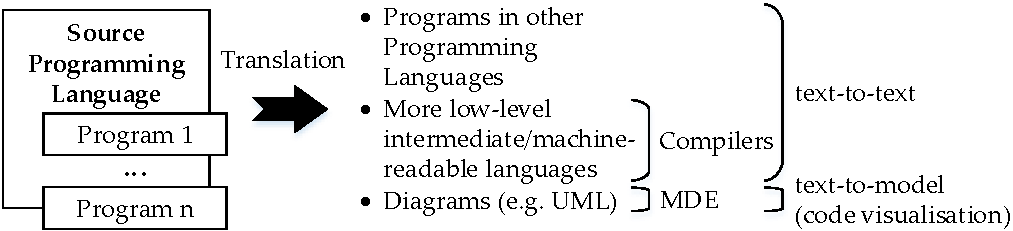
\includegraphics[width=.85\textwidth]{img/software_trans/software_trans2.pdf}
\end{center}
\caption{Types of Software Translations}
\label{fig:sec-compl-software-trans:software_trans_types}
\end{figure}


\subsection{Software Transformations based on Triple Graph Grammars}
\label{sec-compl-software-trans-tgg}
\begin{figure*}[!tb]
\begin{center}
\begin{tikzpicture}
\node[inner sep=0pt] (a) at (0,0) {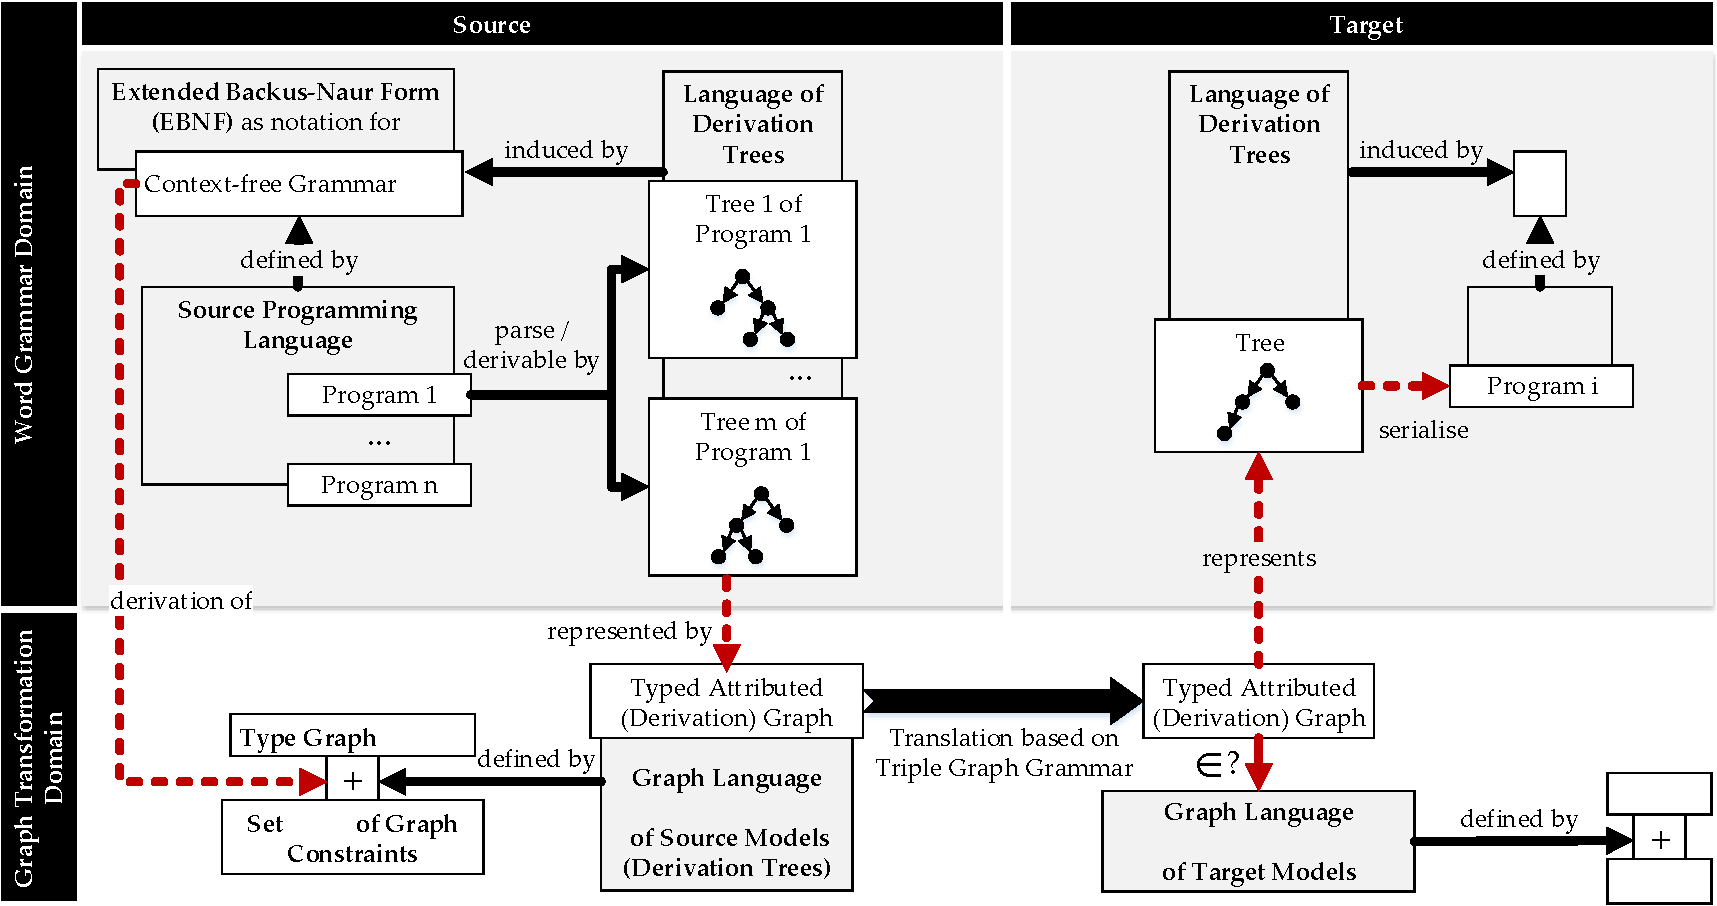
\includegraphics[width=\textwidth]{img/software_trans/software_trans.pdf}};
%\node[inner sep=0pt, right of=a,xshift=8.2cm] (b) {\includegraphics[width=.23\textwidth]{img/ast1.pdf}};
\node[inner sep=0pt] (b) at (-4.05,.95) {\scriptsize{$\Lang^S$}};
\node[inner sep=0pt] (c) at (5.85,1.1) {\scriptsize{$\Lang^T$}};
\node[inner sep=0pt] (d) at (-3.75,2.32) {\scriptsize{$G^S$}};
\node[inner sep=0pt] (e) at (5.85,2.3) {\scriptsize{$G^T$}};
\node[inner sep=0pt] (f) at (-3.7,-2.4) {\scriptsize{$\TG^S$}};
\node[inner sep=0pt] (g) at (-4.6,-3.15) {\scriptsize{$C^S$}};
\node[inner sep=0pt] (h) at (6.95,-2.92) {\scriptsize{$\TG^T$}};
\node[inner sep=0pt] (i) at (6.97,-3.67) {\scriptsize{$C^T$}};
\node[inner sep=0pt] (j) at (-1.1,-3.05) {\scriptsize{$\mathcal{VL}^S$}};
\node[inner sep=0pt] (k) at (3.5,-3.35) {\scriptsize{$\mathcal{VL}^T$}};
\end{tikzpicture}
\end{center}
\caption{Overview of Software Translations based on Triple Graph Grammars}
\label{fig:sec-compl-software-trans:softwaretrans}
\end{figure*}

\cref{fig:sec-compl-software-trans:softwaretrans} illustrates an overview of software translations based on triple graph grammars.
In software translations, programs written in a source programming language $\Lang^S$ are translated into programs (i.e. words) of a target (programming) language $\Lang^T$ (text-to-text translation) or into models of a target visual modelling language $\mathcal{VL}^T$ (text-to-model translation) (cf. \cref{fig:sec-compl-software-trans:software_trans_types}).
We assume that the source (target) word languages $\Lang^S$ ($\Lang^T$) are defined by context-free grammars $G^S$ ($G^T$) where the extended backus-naur form (EBNF) is used as a short-hand notation for context-free grammars in order to define programming languages.
Moreover, we assume that the target visual modelling language $\mathcal{VL}^T$ is a graph language of typed attributed graphs as models and is defined by an attributed type graph $\TG^T$ together with a set of graph constraints $C^T$.
Each context-free grammar induces a language of derivation trees that can be formed over the grammar.
Each derivation tree defines how a specific program (word) can be derived from the grammar.
Therefore, each derivation tree represents a specific program (word) of the language which is defined by the grammar.
Thus, the translation of programs is performed by translating their derivation trees.
In the following we give examples for an EBNF grammar, a derivation tree and the corresponding program which serve as running examples for the subsequent sections.

\begin{figure*}[!tb]
\begin{minipage}[c]{.51\textwidth}
\begin{lstlisting}
PROGRAM: first=CLASS
-----------------------------------------

CLASS  : 'class' name1=STRING (':' e=STR_LST)? '{' (attr1=ATTR)? '}' ('\n' (n1=CLASS | n2=ST))?
STR_LST: name2=STRING (',' n3=STR_LST)?
ATTR   : type=STRING name3=STRING ';' (n4=ATTR)?
-----------------------------------------

NEW    : 'new' cl2=STRING
ACCESS : obj=VAR '.' attr2=STRING
ST     : (a=ASG | p=PRINT | r=READ | i=IF | g=GOTO) ';' ('\n' n5=ST)?
ASG    : (a1=VAR | a2=ACCESS) '=' (a3=VAR | a4=ACCESS | a5=NEW)
PRINT  : 'print' out=ACCESS
READ   : 'read' (in1=VAR | in2=ACCESS)
IF     : 'if' c=COND 'then' body=ST 'end'
COND   : l=VAR ('='|'!=') (r1=STRING | r2=ACCESS | r3=NULL)
GOTO   : 'goto' line=INT
-----------------------------------------

terminal NULL   : 'null'
terminal STRING	: '"'.*'"'
terminal VAR    : ('a'..'z'|'A'..'Z')+
terminal INT    : (0..9)+
\end{lstlisting}
\end{minipage}
\begin{minipage}[c]{.45\textwidth}
\begin{lstlisting}
class "Person" { "String" "name"; "Person" "next"; }
class "Employee" : "Person" { "String" "salary"; }
-----------------------------------------
fst = new "Employee";
lst = fst;
read proceed;
-----------------------------------------
if proceed = "in" then
  read lst."name";
  read lst."salary";
  p = new "Employee";
  lst."next" = p;
  lst = p;
  goto 6;
end;
-----------------------------------------
if proceed = "out" then
  read name;
  current = fst;
  if name = current."name" then
    print current."salary";
  end;
  current = current."next";
  if current != null then
    goto 20;
  end;
  goto 6;
end;
\end{lstlisting}
\end{minipage}
\caption{Xtext EBNF Grammar of language \textit{Conditional-IN-OUT} (left) \& Program of language \textit{Conditional-IN-OUT} (right)}
\label{fig:sec-compl-software-trans:ebnf_xtext}
\end{figure*}

\begin{example}[Xtext EBNF Grammar]
\label{ex:sec-compl-software-trans:xtext_ebnf}
The EBNF grammar in \cref{fig:sec-compl-software-trans:ebnf_xtext} (left) is presented in Xtext notation and defines the ``toy'' programming language \textit{Conditional-IN-OUT}.
Xtext \cite{xtext} uses a special EBNF syntax for specifying context-free grammars of textual domain specific languages.
Xtext is widely used for the definition of programming languages and generates language parsers and editors automatically.

Each line represents a grammar rule.
In language \textit{Conditional-IN-OUT}, programs may \textsf{read} input from the user (line 14), assign it to a (member) variable (\textsf{ACCESS} (line 9)) \textsf{VAR} (line 22) and use the variable in comparisons with \textsf{STRING}s (line 21) and variables as conditions \textsf{COND} (line 16) in \textsf{if}-statements (line 15) in order to \textsf{print} some conditional output to the user (line 13).
Additionally to local variables \textsf{VAR}, data may also be stored in a more structured object-oriented way in member variables of classes.
Each \textsf{PROGRAM} \textsf{first} starts with a class definition (line 1).
Each \textsf{CLASS} (line 4) optionally refers (\textsf{n1}) to the next class or statement \textsf{ST} (\textsf{n2}).
Furthermore, each \textsf{CLASS} has a name (\textsf{name1}) of type \textsf{STRING} and optionally may inherit (reference \textsf{e}) from a set of classes that are given by a comma-separated list \textsf{STR\_LST} of \textsf{STRING}s (line 5) that are given after a colon \textsf{:} in the class definition and represent the class names.
Moreover, each \textsf{CLASS} may refer (\textsf{attr1}) to a set of attributes \textsf{ATTR} as member variables.
Each attribute (line 6) is given by a \textsf{type} and a name (\textsf{name3}), both defined by a \textsf{STRING}, and optionally may refer (\textsf{n4}) to the next attribute separated by a semicolon.
Object creation (line 9) is given by the keyword \textsf{new} followed by the class name (\textsf{cl2}) of the class from which the object is created.
\textsf{ACCESS} (line 10) to a member variable of an object is given by the standard dot-notation with a \textsf{VAR}iable that refers to the object (\textsf{obj}) on the left and the name of the member (\textsf{attr2}) on the right.
Statements \textsf{ST} (line 11) of a \textsf{PROGRAM} are assignments (\textsf{ASG}), \textsf{PRINT}, \textsf{READ}, \textsf{IF}-statements or \textsf{GOTO}s.
Furthermore, each statement \textsf{ST} optionally may refer (\textsf{n5}) to the next statement separated by a semicolon and newline.
Additionally to the statements that we already discussed above, assignments (line 12) are given by the symbol \textsf{=} with a (member) variable (\textsf{a2}) \textsf{a1} on the left and a (member) variable (\textsf{a4}) \textsf{a3} or object creation (\textsf{a5}) on the right.
Furthermore, \textsf{GOTO} statements (line 17) are given by the keyword \textsf{goto} together with the number \textsf{INT} of the \textsf{line} in which the execution of the program should proceed.

In Xtext notation, terminal symbols may be grouped in sorts and defined by so called terminal rules with regular expressions for each sort (lines 20-23).
Sort \textsf{STRING} (line 21) is defined by the regular expression \textsf{'"'.*'"'} allowing sequences of any character that are enclosed by quotation marks.
In contrast to \textsf{STRING}s, variables \textsf{VAR}s (line 22) are given by sequences of alphabetic characters that are not enclosed by quotation marks and \textsf{INT}s (line 23) are defined by sequences of numbers.
Moreover, the sort \textsf{NULL} (line 20) is given by the keyword \textsf{null} which refers to the null object.
\envEndMarker
\end{example}

\begin{example}[Program in language \textit{Conditional-IN-OUT}]
\label{ex:sec-compl-software-trans:prog}
In \cref{fig:sec-compl-software-trans:ebnf_xtext} (right), we present a program of language \textit{Conditional-IN-OUT} from \cref{ex:sec-compl-software-trans:xtext_ebnf}.
Two classes \textsf{Person} and \textsf{Employee} are defined.
\textsf{Person}s have a \textsf{name} and a \textsf{next} \textsf{Person} (line 1).
\textsf{Employees} are a special type of \textsf{Person}s by inheritance and additionally have a \textsf{salary} (line 2).
Lines 4-5 initialise an empty list of \textsf{Employee}s with a new \textsf{Employee} object as the first (\textsf{fst}) and last (\textsf{lst}) list element.
Line 6 reads the user input into variable \textsf{proceed}.
Depending on the user input, either the program asks the user to add a new \textsf{Employee} to the list (lines 8-15) or the program returns the \textsf{salary} of an existing \textsf{Employee} in the list (lines 17-27) where the \textsf{Employee} is identified by his \textsf{name}.
Finally, the program proceeds with line 6 or terminates if the user input differs from \textsf{``in''} or \textsf{``out''}.
\envEndMarker
\end{example}

\begin{figure*}[!tb]
\centering
\includegraphics[width=.47\textwidth]{img/software_trans/ast1.pdf}
\caption{Derivation Tree}
\label{fig:sec-compl-software-trans:ast}
\end{figure*}

\begin{example}[Derivation Tree]
\label{ex:sec-compl-software-trans:der_tree1}
The derivation tree of the program in \cref{ex:sec-compl-software-trans:prog} up to line 3 as induced by the grammar of \cref{ex:sec-compl-software-trans:xtext_ebnf} is presented in graphical notation in \cref{fig:sec-compl-software-trans:ast}.
Non-terminals become nodes in the tree, terminals of sorts \textsf{STRING},\textsf{VAR},\textsf{INT} and \textsf{NULL} become node attributes and references between grammar rules become edges.
Explicit keywords of the language (e.g. \textsf{class}) are not included in the tree.
By following the grammar, in derivation trees, the list of attributes of a class in a program are represented by edge \textsf{:attr1} pointing to the first attribute and edges \textsf{:n4} pointing to the next attribute.
Analogously, the lists of class definitions and the list of inherited classes for each class in a program are represented by edges \textsf{:first}, \textsf{:n1} and \textsf{:e}, \textsf{:n3}.
The complete tree that covers the whole program is given analogously.
\envEndMarker
\end{example}

Given a context-free grammar $G^S$ for source word language $\Lang^S$, then the translation of the induced derivation trees is specified by a triple graph grammar.
By \cref{fig:sec-compl-software-trans:softwaretrans}, each derivation tree is represented by a typed attributed graph in the source domain.
Then, the translation is performed by executing a model transformation on the graph based on the given triple graph grammar.
The result of the translation is a typed attributed graph in the target domain.
For text-to-model translations, the resulting graph is intended to directly serve as the resulting visual model in the target visual modelling language $\mathcal{VL}^T$ of the translation.
For text-to-text translations, the resulting graph is intended to be a representation of a derivation tree which is induced by the target context-free grammar $G^T$ of target word language $\Lang^T$.
The overall result of the text-to-text translation is obtained by flattening (serialising) the tree to a word (program) of the target language $\Lang^T$.
We demonstrate the graph-based approach for software translations by a translation of programs of language \textit{Conditional-IN-OUT} from \cref{ex:sec-compl-software-trans:xtext_ebnf} into UML class diagrams in \cref{ex:sec-compl-software-trans:trans}.
At first, we present the attributed type graphs of the source (\textit{Conditional-IN-OUT}) and target (class diagrams) domains of the translation in \cref{ex:sec-compl-software-trans:type_graphs}.

\begin{figure*}[!tb]
\centering
\includegraphics[width=.98\textwidth]{img/software_trans/tg.pdf}
\caption{EBNF Type Graph of Grammar \textit{Conditional-IN-OUT} (\textit{Root}+\textit{Statements}+\textit{Classes}) \& Triple Type Graph (\textit{Source} $\gets$ \textit{Correspondence} $\to$ \textit{Target})}
\label{fig:sec-compl-software-trans:tg_ebnf}
\end{figure*}

\begin{example}[Attributed Type Graphs]
\label{ex:sec-compl-software-trans:type_graphs}
\cref{fig:sec-compl-software-trans:tg_ebnf} illustrates both the attributed type graph of source language \textit{Conditional-IN-OUT} and the type graph of the target visual modelling language of UML class diagrams.
The type graph of \textit{Conditional-IN-OUT} is given by boxes \textit{Root},\textit{Statements} and \textit{Classes}.
The graph represents the structure of the \textit{Conditional-IN-OUT} grammar in \cref{fig:sec-compl-software-trans:ebnf_xtext} (left) where each grammar rule becomes a node in the graph and references between rules become edges or node attributes.
The type graph of class diagrams is given by box \textit{Target}.
Each diagram may have several \code{Class} nodes with a name (node attribute \code{cname}) of type \code{STRING} for each class.
Furthermore, each class may have several attributes (\code{Attr} nodes) each assigned by an \code{attr} edge.
Each attribute has a \code{type} and a name (node attribute \code{aname}) both of type \code{STRING}.
Moreover, there may be explicit inheritance relationships (\code{i} edges) and associations (\code{assoc} edges) between classes.
\envEndMarker
\end{example}

\begin{example}[Translation of \textit{Conditional-IN-OUT}]
\label{ex:sec-compl-software-trans:trans}
Each program of language \textit{Conditional-IN-OUT} from \cref{ex:sec-compl-software-trans:xtext_ebnf} is translated into an UML class diagram by transforming each class definition in the program into a \code{Class} node with optional attributes, association and inheritance relationships in the class diagram.
The translation of programs is performed by translating their derivation trees and specified by the triple graph grammar $\TGG=(\varnothing, P)$ with empty start graph $\varnothing$ and triple graph productions $P$ as given in \cref{fig:sec-compl-software-trans:rules}.
The triple graph production rules are typed over the triple type graph (\textit{Source} $\gets$ \textit{Correspondence} $\to$ \textit{Target}) in \cref{fig:sec-compl-software-trans:tg_ebnf}.
The triple type graph is given by boxes \textit{Classes} for \textit{Source} and \textit{Target} as described in \cref{ex:sec-compl-software-trans:type_graphs} together with a \textit{Correspondence} part which maps 
\begin{enumerate*}
\item \code{CLASS}es in programs to \code{Class} nodes in class diagrams (via correspondence nodes \code{CC}),
\item the names of inherited classes (\code{STR\_LST} nodes) to \code{Class} nodes (via \code{SC} correspondence nodes), and
\item class attributes (\code{ATTR} nodes) to class attributes (\code{Attr} nodes) (via \code{AA} correspondence nodes).
\end{enumerate*}
The production rules are presented in short-hand notation.
The elements of each triple rule are partitioned into the following three parts:
\begin{enumerate*}
\item source- (\textit{Conditional-IN-OUT}),
\item target-domain (UML class diagram) of the translation, and
\item correspondence part which maps elements from source to target and vice versa.
\end{enumerate*} 
For each rule $\LHS \to \RHS$ with left-hand side $\LHS$ and right-hand side $\RHS$, the $\LHS$ consists of all elements that are not marked with \textsf{++} whereas the $\RHS$ additionally consists of all elements that are marked with \textsf{++} and therefore, that are created when applying the rule to a $\LHS$ context.
Moreover, each rule is equipped with a negative application condition ($\NAC$) which restricts the rule application by describing a graph structure that is forbidden to exist for applying the rule.
For example, rule \textit{1:C2C} in \cref{fig:sec-compl-software-trans:rules} simultaneously creates a \textsf{CLASS} and a \textsf{Class} node with name \textsf{n} in the source and target domain with correspondence node \textsf{:CC} between both but only if the class diagram not already contains a \textsf{Class} node of the same name.
While the triple rules specify the translation, the translation itself is performed by applying operational forward translation rules that are derived from the triple rules.
Thus, from each rule $p \in P$, an operational forward translation rule $p_\FT$ is automatically derived.
For technical details we refer to Def. 7.29 in \cite{FAGT2} while the idea is rather straightforward.
Given a triple rule $p$, then the corresponding forward translation rule $p_\FT$ of $p$ translates those elements $E$ that are created by $p$ in the source domain into those elements $E'$ that are created by $p$ in the target domain together with the created correspondence part by adding elements $E'$ to elements $E$.
Moreover, the translation rule marks the translated elements as being translated in order to prevent a second translation of those elements.
In the following we give short descriptions for the forward translations rules of the triple rules in \cref{fig:sec-compl-software-trans:rules}.
The major challenges of the translation include:
\begin{enumerate*}
  \item the mapping of the list of class attributes for each class in a program to a star of attributes around the corresponding class node in the class diagram (rules \textit{2} \& \textit{3}),
  \item the mapping of the list of names of inherited classes for each class in a program to explicit inheritance relationships between actual class nodes in the class diagram (rules \textit{4} \& \textit{5}), and
  \item the mapping of implicit associations between classes in a program as given by the types of class attributes to explicit association relationships between actual class nodes in the class diagram (rules \textit{6} to \textit{10}).
\end{enumerate*}

\begin{figure*}[!tb]
\centering
\includegraphics[width=\textwidth]{img/software_trans/rules.pdf}
\caption{Triple Graph Rules for Translation of Derivation Trees of Grammar \textit{Conditional-IN-OUT}}
\label{fig:sec-compl-software-trans:rules}
\end{figure*}

\begin{enumerate}
  \item Rule \textit{1:C2C}$_\FT$ translates a \textsf{CLASS} of name \textsf{n} in a program into a corresponding \textsf{Class} node with name \textsf{n} in the class diagram but only if there does not already exist a \textsf{Class} node with the same name (cf. $\NAC_1$).
  \item Rule \textit{2:A2A}$_{1,\FT}$ assumes that a \textsf{CLASS} in a program is already translated into a corresponding \textsf{Class} node in the class diagram.
  The rule translates the first class attribute (\textsf{:ATTR}) with name \textsf{n} of \textsf{:CLASS} into a corresponding attribute (\textsf{:Attr}) with name \textsf{n} of node \textsf{:Class} in the class diagram but only if node \textsf{:Class} does not already contain an attribute with the same name (cf. $\NAC_2$).
  \item Rule \textit{3:A2A}$_{2,\FT}$ translates the next attribute of the class into a corresponding attribute in the class diagram but analogously to rule \textit{2:A2A}$_{1,\FT}$, only if the correponding \textsf{Class} node in the diagram does not already contain an attribute with the same name (cf. $\NAC_3$).
  \item Rule \textit{4:S2I}$_{1,\FT}$ translates the name \textsf{n2} of the first inherited class for class \textsf{n1} in a program into an inheritance edge between the corresponding \textsf{Class} nodes in the class diagram but only if there does not already exist an inheritance edge between both nodes (cf. $\NAC_4$).
  \item Analogously to rule \textit{3:A2A}$_{2,\FT}$ for rule \textit{2:A2A}$_{1,\FT}$, rule \textit{5:S2I}$_{2,\FT}$ translates the name \textsf{n2} of the next inherited class for class \textsf{n1} into an inheritance edge between the corresponding \textsf{Class} nodes in the class diagram but only if there does not already exist an inheritance edge between both nodes (cf. $\NAC_5$).
  \item Rule \textit{10:T2T}$_{3,\FT}$ translates the type \textsf{t1} of a class attribute in a program into the same type of the corresponding attribute in the class diagram but only if type \textsf{t1} is not the name of a \textsf{CLASS} in the program and the attribute in the diagram does not already have a type \textsf{t2} (cf. $\NAC_{10a} \wedge \NAC_{10b}$).
  \item In contrast to rule \textit{10:T2T}$_{3,\FT}$, if type \textsf{t1} is the name of a \textsf{CLASS} in the program, then:
  \begin{enumerate}
    \item If \textsf{t1} is the name of the class of the class attribute and the corresponding \textsf{Class} node in the class diagram does already have a reflexive association (edge \textsf{:assoc}), then rule \textsf{6:T2T}$_1$ simply translates \textsf{t1} into the same type of the corresponding attribute in the class diagram but only if the attribute does not already have a type \textsf{t2} (cf. $\NAC_6$).
    \item If \textsf{t1} is the name of the class of the class attribute, then rule \textsf{7:T2A}$_1$ translates \textsf{t1} into the same type of the corresponding attribute together with a reflexive association for the corresponding \textsf{Class} node in the class diagram but only if the attribute does not already have a type \textsf{t2} and the \textsf{Class} node does not already have a reflexive association (cf. $\NAC_{7a} \wedge \NAC_{7b}$).
    \item If \textsf{t1} is not the name of the class of the class attribute but the name of another class in the program and there already exists an association between the corresponding \textsf{Class} nodes in the class diagram, then rule \textsf{8:T2T}$_2$ simply translates \textsf{t1} into the same type of the corresponding attribute in the class diagram but only if the attribute does not already have a type \textsf{t2} (cf. $\NAC_8$).
    \item If \textsf{t1} is not the name of the class of the class attribute but the name of another class in the program, then rule \textsf{9:T2A}$_2$ translates \textsf{t1} into the same type of the corresponding attribute together with an association between the corresponding \textsf{Class} nodes in the class diagram but only if the attribute does not already have a type \textsf{t2} and there does not already exist an association between the two \textsf{Class} nodes (cf. $\NAC_{9a} \wedge \NAC_{9b}$).
  \end{enumerate}
\end{enumerate}

\begin{figure*}[!tb]
\centering
\includegraphics[width=.48\textwidth]{img/software_trans/result.pdf}
\caption{Result Graph}
\label{fig:sec-compl-software-trans:result}
\end{figure*}

The result of translating the derivation tree in \cref{ex:sec-compl-software-trans:der_tree1} by the forward translation rules from above is given by the typed attributed graph in \cref{fig:sec-compl-software-trans:result}.
The graph serves as a class diagram model in the target domain of the translation.
The list of attributes \textsf{name} and \textsf{next} of class \textsf{Person} becomes a star of attributes around the corresponding class node in the class diagram.
Furthermore, the implicit inheritance and association relationships between classes in the program become explicit edges in the class diagram.
\envEndMarker
\end{example}

\begin{remark}[Application Conditions in Translation]
The rules in \cref{ex:sec-compl-software-trans:trans} make extensive use of negative application conditions (NACs) in order to control the translation.
While the negative application conditions $\NAC_{7b},\NAC_{9b}$ and $\NAC_{10a}$ ensure that at most one rule of rules \textit{6} to \textit{10} as applicable to a given context at the same time, the other application conditions rather define restrictions of the target language of the translation, i.e., restrictions that need to be satisfied by each class diagram which results from a translation of a \textit{Conditional-IN-OUT} program.
\begin{enumerate*}
\item $\NAC_1$ ensures that each resulting class diagram does not contain two classes with the same name,
\item $\NAC_2$ and $\NAC_3$ ensure that each resulting class diagram does not contain a class with two or more class attributes having the same name,
\item $\NAC_4$ and $\NAC_5$ ensure that each resulting class diagram does contain at most one inheritance edge between each two classes,
\item $\NAC_6,\NAC_{7a},\NAC_8,\NAC_{9a}$ and $\NAC_{10b}$ ensure that each resulting class diagram does contain at most one type for each class attribute, and
\item $\NAC_{7b}$ and $\NAC_{9b}$ ensure that each resulting class diagram does contain at most one association between each two classes. \envEndMarker
\end{enumerate*}
\end{remark}

\subsection{Completeness Problem of Software Transformations}
\label{sec-compl-software-trans-prob}
As illustrated in \cref{fig:sec-compl-software-trans:softwaretrans}, our approach of translating programs of a programming language $\Lang^S$ is to translate their derivation trees as induced by the word grammar $G^S$ of $\Lang^S$.
Each derivation tree is represented by a typed attributed graph in the source graph language $\mathcal{VL}^S$ of derivation trees and translated by performing a model transformation based on a given triple graph grammar.
The result is a typed attributed graph in the target modelling (graph) language $\mathcal{VL}^T$.
Furthermore, we assume that the source (target) graph language is defined by a type graph $\TG^S$ ($\TG^T$) together with a set $C^S$ ($C^T$) of graph contraints.

\begin{definition}[Graph Language over Type Graph \& Constraints]
\index{language!$\Lang(C)$ over graph constraints}
Given a type graph $\TG$ and a set $C$ of graph constraints that are typed over $\TG$.
Then, the \emph{graph language over $\TG$ and $C$} is given by $\Lang(\TG,C)=\{G \mid \text{graph }G\text{ is typed over }\TG,G \models C\}$ all graphs $G$ that are typed over $\TG$ and that satisfy the constraints $C$.
\envEndMarker
\end{definition}

The translation is syntactically complete, if all derivation trees of $G^S$ can be completely translated.
Intuitively, a derivation tree is completely translated, if all nodes and edges of the tree are translated exactly once.
Since, the translation of derivation trees is based on the translation of their graph representations, it is required that the language $\Der(G^S)$ of derivation trees of  $G^S$ is isomorphic to the graph language $\Lang(\TG^S,C^S)$ of their graph representations (cf. \cref{sec-compl-software-trans-mapping,thm:sec-compl-software-trans:equ_lang_der}).
Thus, each tree in $\Der(G^S)$ is represented by exactly one graph in $\Lang(\TG^S,C^S)$ and each graph in $\Lang(\TG^S,C^S)$ represents exactly one derivation tree in $\Der(G^S)$.

\begin{definition}[Isomorphism of Derivation Tree Languages]
\label{def:sec-compl-software-trans-prob:iso}
\index{language!of derivation trees!isomorphism}
Given a context-free word grammar $G$ with induced language $\Der(G)$ of derivation trees.
Let $\Lang(\TG,C)$ be a graph language of derivation trees over type graph $\TG$ and graph constraints $C$.
\emph{Languages $\Der(G)$ and $\Lang(\TG,C)$ are isomorphic}, if there exists a bijection $m\colon \Der(G) \to \Lang(\TG,C)$ between both.
\envEndMarker
\end{definition}

By \cref{def:comp_soft_trans}, a software translation is syntactically complete if each source derivation graph $G^S \in \Lang(\TG^S,C^S)$ can be completely translated via a model transformation sequence in the sense that all elements of the graph are translated exactly once by changing their translation attributes from $\False$ to $\True$.

\begin{definition}[Syntactical Completeness of Software Translations]
\label{def:comp_soft_trans}
\index{software transformation!completeness}
Given a context-free word grammar $G^S$ for source language $\Lang^S$ with induced language $\Der(G^S)$ of derivation trees.
Let $\TG=(\TG^S \gets \TG^C \to \TG^T)$ be a triple type graph with $\Lang(\TG^S,C^S)$ being the graph language of derivation trees isomorphic to $\Der(G^S)$. 
Furthermore, let $\TGG=(\varnothing,\TR)$ be a triple graph grammar typed over $\TG$ with derived forward translation rules $\TR_\FT$ that specifies the model transformation of graphs in $\Lang(\TG^S,C^S)$ into graphs of target graph language $\Lang(\TG^T,C^T)$ based on forward translation rules $\TR_\FT$.
\emph{The translation is syntactically complete}, if for each derivation graph $G^S \in \Lang(\TG^S,C^S)$ there is a model transformation sequence $(G^S,G_0 \Trans{\tr^*_\FT} G_n,G^T)$ based on forward translation rules $\TR_\FT$ with $G_0=(\Att^\False(G^S) \gets \varnothing \to \varnothing)$ and $G_n=(\Att^\True(G^S) \gets G^C \to G^T)$.\envEndMarker
\end{definition}

From the setting for translations in \cref{fig:sec-compl-software-trans:softwaretrans} and from \cref{def:comp_soft_trans,fact:comp_soft_trans}, the following problems arise concerning the completeness and correctness of software translations.

\begin{problem}[Syntactical Completeness \& Correctness of Software Translations]
\label{prob:scst}
\begin{enumerate}
  \item \label{item:scst1} Syntactical Completeness \& Correctness: Given a context-free word grammar $G$ with induced language $\Der(G)$ of derivation trees.
  How to derive a graph language $\Lang(\TG,C)$ of derivation trees from $G$ that is isomorphic to $\Der(G)$?
  \item \label{item:scst2} Syntactical Completeness: How to verify the language inclusion $\Lang(\TG^S,C^S) \subseteq \Lang(\TGG)^S$ (domain completeness)?
  \item \label{item:scst3} Syntactical Correctness: How to ensure that the resulting graphs of a translation are actually graphs of the target graph language $\Lang(\TG^T,C^T)$, i.e., $\Lang(\TGG)^T \subseteq \Lang(TG^T,C^T)$ (domain correctness)?
  \item \label{item:scst4} Syntactical Completeness \& Correctness: Given verification techniques for the language inclusion problems in \cref{item:scst2,item:scst3}.
  Are the techniques applicable to the derived type graph $\TG$ and the derived set of graph contraints $C$ of \cref{item:scst1}?\envEndMarker
\end{enumerate}
\end{problem}

Beside the completeness problem, \cref{fig:sec-compl-software-trans:softwaretrans} also brings forth the correctness problem of software translations in \cref{prob:scst,item:scst3}.
Therefore, are the resulting graphs 
\begin{enumerate*}
\item models of the target language in text-to-model translations, or
\item actually representations of derivation trees of the target programming language in text-to-text translations such that they can be serialised to target programs?
\end{enumerate*}
While the correctness problem remains subject of future work under the notion of domain correctness, we furthermore concentrate on the completeness problem based on the notion of domain completeness.
While the syntactical completeness of software translations in the graph world itself, i.e., the language inclusion in \cref{fact:comp_soft_trans}, can be verified by means of the existing verification techniques for domain completeness (cf. \cref{prob:scst,item:scst2}), it remains to close the gap between the word grammar and graph world (cf. \cref{prob:scst,item:scst1}) such that the verification techniques for domain completeness are applicable (cf. \cref{prob:scst,item:scst4}).
The gap is closed by presenting a mapping from context-free (EBNF) grammars $G$ to attributed EBNF type graphs $\TG$ together with EBNF graph constraints $C$ in \cref{sec-compl-software-trans-mapping} such that the induced language $\Der(G)$ of derivation trees is isomorphic to the graph language $\Lang(\TG,C)$ of derivation trees (cf. \cref{sec-compl-software-trans-mapping,thm:sec-compl-software-trans:equ_lang_der}).
Furthermore, we use several extensions of the verification techniques for domain completeness in view of the derived EBNF type graphs $\TG$ and EBNF graph constraints $C$ for verifying the completeness of the translation in \cref{sec-compl-software-trans-tgg,ex:sec-compl-software-trans:trans}.
The extension includes
\begin{enumerate*}
\item recursive graph constraints from \cref{sec-dc-general-rec}, and
\item domain restrictions from \cref{sec-dc-general-res}.
\end{enumerate*}
While recursive graph constraints are used for the definition of EBNF graph constraints $C$ in \cref{sec-compl-software-trans-mapping,def:sec-compl-software-trans:ebnf_constraints}, domain restrictions are necessary for the translation in \cref{sec-compl-software-trans-tgg,ex:sec-compl-software-trans:trans} which only covers those parts of a derivation tree which are related to class definitions in a program.
Thus, a restriction of the graph language of derivation trees to a sub-language covering the class definitions only is required for verifying the completeness of the translation, called domain completeness under restrictions (cf. \cref{sec-dc-general-res,def:sec-dc-general-res:dc_prob}).

\subsection{From EBNF Grammars to Attributed Type Graphs \& Graph Constraints}
\label{sec-compl-software-trans-mapping}
In \cite{DBLP:conf/icmt/0001GNEBMPEE14}, Xtext is used for the definition of a source and target satellite procedure language for software translations between both.
In the following we take (abstract) syntax trees of programs written in a programming language $L$ and derivation trees of a context-free grammar defining this language $L$ as synonyms.
We formalise the notion of Xtext EBNF grammars in \cref{def:sec-compl-software-trans:ebnf}, called EBNF grammars with labels.
Labelled elements of the grammar are included in derivation trees whereas unlabelled elements are not. 
In particular, a separation of the terminals in the set $T$ and a family of sets $(C_s)_{s \in S}$ allows a distinction of which terminals are included in derivation trees and which are not.
As software translations aim at the translation of the derivation tree of a program's syntax, this distinction allows to specify which terminals are relevant for the translation and which are not.
The terminals $T$ are not included in derivation trees whereas the elements of the family of sets $(C_s)_{s \in S}$ may be included where each sort $s \in S$ represents a terminal rule in the Xtext grammar and the corresponding carrier set $C_s$ is the set of all words that are derivable from the regular expression of the terminal rule.

\begin{definition}[EBNF Grammar with Labels]
\label{def:sec-compl-software-trans:ebnf}
\index{EBNF grammar!with labels}
An \emph{EBNF grammar $G=(N,n_S,T,L,S,(C_s)_{s \in S},P)$ with labels} is given by
\begin{enumerate}
  \item A set $N$ of non-terminals,
  \item A non-terminal $n_S \in N$ as start symbol,
  \item a set $T$ of terminals,
  \item a set $L$ of labels,
  \item \label{item:sec-compl-software-trans:ebnfA5}a set $S$ of sorts disjoint from the set $N$,
  \item a family of carrier sets $(C_s)_{s \in S}$ with a carrier set $C_s$ for each sort $s \in S$ ($C_s$ defines the terminals for $s$),
  \item a set $P$ of production rules $p\colon n \in N \to R^*$ with a non-terminal $n$ as the left-hand-side (LHS) of the rule and an (empty) sequence $R^*$ as the right-hand-side (RHS) where $R=(L \times N) \cup T \cup (L \times S)$ such that:
  \begin{enumerate}
    \item \label{item:sec-compl-software-trans:ebnfA1}The labelling is unique.
    Thus, let $|p|$ be the amount of label occurrences in production $p$ and $L(p)$ be the set of labels that occur in $p$, then for $P$ it holds that $+_{p \in P} (|p|)=|\cup_{p \in P} (L(p))|$.
    \item \label{item:sec-compl-software-trans:ebnfA2}All labels are used in productions, i.e., $|L|=|\cup_{p \in P} (L(p))|$.
  \end{enumerate} 
    
  The terminals $T$ are called unlabelled whereas $L \times N$ are labelled references to non-terminals $N$ and $L \times S$ are labelled references to sorts $S$ where each sort $s \in S$ represents a set of terminals $C_s$.
  For productions with an empty sequence as RHS we write $n \to \epsilon$, and
  \item \label{item:sec-compl-software-trans:ebnfA8}the start symbol is not target of a reference.
  Therefore, for all productions $p \in P$ with $p\colon n \to R^*$, it holds that $(l,n_s) \in (L \times N)$ does not occur in the RHS $R^*$ of $p$.\envEndMarker
\end{enumerate}
\end{definition}

\cref{def:sec-compl-software-trans:ebnf,item:sec-compl-software-trans:ebnfA5,item:sec-compl-software-trans:ebnfA1,item:sec-compl-software-trans:ebnfA2} enable the definition of the source and target of each labelled reference in an EBNF grammar based on its label $l \in L$ by well-defined functions $s\colon L \to N$ for the source and $t\colon L \to N \cup S$ for the target.

\begin{definition}[Source \& Target of Labels]
\label{def:sec-compl-software-trans:st_labels}
\index{EBNF grammar!with labels!source}
\index{EBNF grammar!with labels!target}
Let $L$ be the labels and $P$ be the productions of an EBNF grammar with labels.
\emph{The source $s\colon L \to N$ of a label $l \in L$} is given by $s(l):=n$ where $(l,n') \in (L \times N)$ occurs in the RHS $R^*$ of a production $p \in P$ with $p\colon n\to R^*$.
\emph{The target $t\colon L \to N \cup S$ of a label $l \in L$} is given by
\begin{center}
$t(l):=\begin{cases}
n' & \quad \text{if } (l,n') \in (L \times N) \text{ occurs in } R^*\\
   & \quad \text{ of a production } p \in P \text{ with } p\colon n \to R^*\\
s  & \quad \text{if } (l,s) \in (L \times S) \text{ occurs in } R^*\\
   & \quad \text{ of a production } p \in P \text{ with } p\colon n \to R^*\\
\end{cases}$
\end{center}
\envEndMarker
\end{definition}

\begin{remark}[Notational Abbreviations]
\label{rem:sec-compl-software-trans:abbr}
In addition to the formal EBNF notation in \cref{def:sec-compl-software-trans:ebnf}, the notation for alternatives in $N \to R_1(R_2|R_3)R_4$ inductively abbreviates the two production rules $N \to R_1R_2R_4$ and $N \to R_1R_3R_4$.
Furthermore, the quantification via the optional operator $?$ in $N \to R_1(R_2)?R_3$ inductively abbreviates the two productions $N \to R_1R_3$ and $N \to R_1R_2R_3$.
\envEndMarker
\end{remark}

\begin{remark}[Context-Free Grammars]
\label{rem:sec-compl-software-trans:ebnf}
Note that \cref{def:sec-compl-software-trans:ebnf} coincides with the classical definition of context-free grammars in two forms.
\begin{enumerate}
  \item \cref{def:sec-compl-software-trans:ebnf} coincides with the classical notion for $T=\varnothing$ and when defining for each terminal $t$ a sort $s_t \in S$ with carrier set $C_{s_t}=\{t\}$ except that an additional unique labelling is required for each occurrence of a non-terminal or sort in the RHS of a production.
  \item \label{item:sec-compl-software-trans:ebnf2}\cref{def:sec-compl-software-trans:ebnf} coincides with the classical notion for $S=\varnothing$.\envEndMarker
\end{enumerate}
For each classical context-free grammar that does not satisfy restriction \cref{def:sec-compl-software-trans:ebnf,item:sec-compl-software-trans:ebnfA8}, the restriction can be bypassed by adding a production to the grammar with a new start symbol as LHS and the old start symbol as RHS without changing the language that is induced by the grammar. 
\end{remark}

\begin{example}[EBNF Grammar with Labels]
\label{ex:sec-compl-software-trans:ebnf}
Each line in lines 1-17 of the EBNF grammar in \cref{sec-compl-software-trans-tgg,ex:sec-compl-software-trans:xtext_ebnf} represents a grammar rule of the form LHS:RHS where the LHS of the rule consists of exactly one non-terminal and the RHS is a sequence of unlabelled terminals and labelled references to non-terminals or sorts.
For example, in line 4, \textsf{class},\textsf{':'},\textsf{\{} and \textsf{\}} are unlabelled terminals whereas \textsf{attr1=ATTR} is a reference to non-terminal \textsf{ATTR} with label \textsf{attr1} and \textsf{name1=STRING} is a reference to sort \textsf{STRING} with label \textsf{name1}.
The sorts are given by Xtext terminal rules in lines 20-23.

Based on \cref{def:sec-compl-software-trans:ebnf}, the formal definition of the grammar is given by:

\begin{enumerate}
  \item The set $N$ of non-terminals that are given by the LHSs of the grammar rules with $N=\{PROGRAM,CL\_LST,CLASS,STR\_LST,ATTR,$ $NEW,ACCESS,ST\_LST,ST,ASG,PRINT,$ $READ,IF,COND,GOTO\}$,
  \item the first rule $PROGRAM$ as start symbol,
  \item the set $T$ of terminals that are given by the words enclosed by quotes in the RHSs of the rules with $T=\{\texttt{\textbackslash n},class,:,\{,\},,,;,new,.,=,print,read,if,then,end,!=,goto\}$,
  \item the set $L$ of labels that are given by the names of the references in the RHSs of the rules with $L=\{first,cl1,n1,n2,name1,e,attr1,name2,n3,type,$ $name3,n4,cl2,obj,attr2,st,n5,a,p,r,i,g,a1,a2,a3,$ $a4,a5,out,in1,in2,c,body,l,r1,r2,r3,line\}$,
  \item the sorts that are given by the terminal rules with $S=\{NULL,STRING,VAR,INT\}$,
  \item the carrier sets that are given by the sets of all words that are derivable from the regular expressions of the corresponding terminal rules with $C_{STRING}=\{w \mid w \text{ is derivable from '"'} .^* \text{'"'}\}$, $C_{VAR}=\{w \mid w \text{ is derivable from } ('a'..'z'|'A'..'Z')+\}$, $C_{INT}=\{w \mid w \text{ is derivable from } (0..9)+\}$ and $C_{NULL}=\{null\}$, and
  \item the following productions by considering the notational abbreviations in \cref{rem:sec-compl-software-trans:abbr}:
  \begin{enumerate}
    \item[a)] $PROGRAM \to (first,CL\_LST)$,
    \item[b)] $CL\_LST \to (cl1,CLASS)$,
    \item[c)] $CL\_LST \to (cl1,CLASS)\ \texttt{\textbackslash n}\ (n1,CL\_LST)$,
    \item[d)] $CL\_LST \to (cl1,CLASS)\ \texttt{\textbackslash n}\ (n2,ST\_LST)$,
    \item[e)] $CLASS \to class\ (name1,STRING)\ \{\ \}$,
    \item[f)] $CLASS \to class\ (name1,STRING)\ $ $\{\ (attr1,ATTR)\ \}$,
    \item[g)] $CLASS \to class\ (name1,STRING)\ :\ (e,STR\_LST)\ \{\ \}$,
    \item[h)] $CLASS \to class\ (name1,STRING)\ :\ (e,STR\_LST)\ \{\ (attr1,ATTR)\ \}$,
    \item[i)] $STR\_LST \to (name2,STRING)$,
    \item[j)] $STR\_LST \to (name2,STRING)$ $\ ,\ (n3,STR\_LST)$,
    \item[k)] $ATTR \to (type,STRING)\ (name3,STRING)\ ;$,
    \item[l)] $ATTR \to (type,STRING)\ (name3,STRING)\ ;$ $\ (n4,ATTR)$, and
    \item[m)] the productions for the rules in lines 8 to 17 are defined analogously.
%     \item[a)] $ST\_LST \to (s,ST)\ ;$,
%     \item[b)] $ST\_LST \to (s,ST)\ ;\ n\ (next,ST\_LST)$,
%     \item[c)] $ST \to (i,IF)$,
%     \item[d)] $ST \to (p,PRINT)$,
%     \item[e)] $ST \to (r,READ)$,
%     \item[f)] $PRINT \to print\ (out,STRING)$,
%     \item[g)] $READ \to read\ (in,VAR)$,
%     \item[h)] $IF \to if\ <\ (c,COND)\ >\ then\ (body,ST)$, and
%     \item[i)] $COND \to (left,VAR)\ =\ (right,STRING)$.
  \end{enumerate}
\end{enumerate}
Note that the set $S$ of sorts is disjoint from the set $N$ of non-terminals, the labelling is unique and all labels are used in productions (cf. \cref{def:sec-compl-software-trans:ebnf,item:sec-compl-software-trans:ebnfA1,item:sec-compl-software-trans:ebnfA2}).
This allows the definition of the source and target of label \textsf{name1} with $s(name1)=CLASS$ and $t(name1)=STRING$ (cf. \cref{def:sec-compl-software-trans:st_labels}).
The sources and targets of the other labels are given analogously.
Furthermore, the start symbol is not target of a reference (cf. \cref{def:sec-compl-software-trans:ebnf,item:sec-compl-software-trans:ebnfA8}).
\envEndMarker
\end{example}

Software translations are performed by translating derivation trees of programs that are induced by the underlying grammar of the programming language to models of the target language.
\cref{def:sec-compl-software-trans:lang_der} defines the language of derivation trees that are induced by an EBNF grammar.
The root node of each derivation tree is the start symbol of the grammar, the internal nodes are non-terminals whereas the leafs are non-terminals or terminals $(C_s)_{s \in S}$ of sorts $S$.
Note that by \cref{def:sec-compl-software-trans:lang_der,item:sec-compl-software-trans:lang_der2}, terminals $T$ of the grammar are not contained in derivation trees making them to a special type of abstract syntax trees of programs where not all details of a grammar are reflected in the trees (cf. concrete syntax trees).

\begin{definition}[Language of Derivation Trees]
\label{def:sec-compl-software-trans:lang_der}
\index{language!of derivation trees}
Let $G=(N,n_s,T,L,S,(C_s)_{s \in S},P)$ be an EBNF grammar with labels.
Then, \emph{the language $\Der(G):=trees(n_S)$ of derivation trees of $G$} is inductively defined by all trees $trees(n_S)$ with root node $n_S$ and:
\begin{enumerate}
  \item $trees(\epsilon)=\{\epsilon\}$,
  \item \label{item:sec-compl-software-trans:lang_der2}$trees(t \in T)=\{\epsilon\}$,
  \item $trees((l,s) \in (L \times S))=\cup_{t \in C_s}\{(l,t)\}$,
  \item $trees((l,n) \in (L \times N))=\cup_{m \in trees(n)}\{(l,m)\}$, and
  \item $trees(n \in N)=\cup_{p \in P'}trees(r_n) \circ \ldots \circ trees(r_1) \circ \{n\}$, for $p\colon n \to r_1 \ldots r_n$ and $P \supseteq P'=\{p\colon n \to R^* \mid p \in P \text{ for some arbitrary }R^*\}$.\envEndMarker 
\end{enumerate}
\end{definition}

\begin{example}[Derivation Tree]
\label{ex:sec-compl-software-trans:der_tree}
Below, the derivation tree of the program in \cref{sec-compl-software-trans-tgg,ex:sec-compl-software-trans:prog} up to line 3 is presented in formal notation by following \cref{def:sec-compl-software-trans:lang_der}.
The corresponding visual graph-like notation is presented in \cref{sec-compl-software-trans-tgg,ex:sec-compl-software-trans:der_tree1}.
 
\begin{lstlisting}[frame=none,language=pseudocode]
PROGRAM (first, CL_LST (cl1, CLASS (name1, "Person") (attr1, ATTR (type, "String") (name3, "name") (n4, ATTR (type, "Person") (name3, "next")))) (n1, CL_LST (cl1, CLASS (name1, "Employee") (e, STR_LST (name2, "Person")) (attr1, ATTR (type, "String) (name3, "salary"))) (n2, ...)))
\end{lstlisting}

The complete tree that covers the whole program is given analogously.
Note that the keywords of the language (terminals $T$ of the grammar) are not contained in the tree.
\envEndMarker
\end{example}

\begin{remark}[Visual Notation of Graphs]
\label{rem:sec-compl-software-trans:vis_graphs}
Note that the graphs in \cref{ex:sec-compl-software-trans:der_tree} are presented in visual notation.
The type of each node and edge is indicated by a preceeding colon.
Thus, the notation \textsf{:n} means that the node or edge is of type $n$.
Technically, the typing of a node (edge) \textsf{:n} is given by a mapping from that node (edge) to node (edge) $n$ in the type graph along the given type morphism of the typed graph containing this node (edge) (cf. \cref{def:sec-compl-software-trans:ebnf_typegraph}).
Furthermore, for node attributes we do not use the explicit E-graph notation but visualise them directly with attribute name and value inside the corresponding nodes.
\envEndMarker
\end{remark}

\begin{remark}[Language of Derivation Trees]
In \cref{def:sec-compl-software-trans:lang_der}, operation $\circ$ is the concatenation of words with $\epsilon$ being the empty word, i.e., $w \circ \epsilon=\epsilon \circ w=w$ for all words $w$.
The concatenation of sets of words $W' \circ W=\{w' \circ w \mid w \in W, w' \in W'\}$ is given by all possible concatenations of words.
Note that \cref{def:sec-compl-software-trans:lang_der} does not coincide with the classical notion of derivation trees (concrete syntax trees) of context-free grammars, not even if \cref{rem:sec-compl-software-trans:ebnf,item:sec-compl-software-trans:ebnf2} is assumed, since, terminals $T$ are not represented in the trees.
\envEndMarker
\end{remark}

\begin{remark}[Decidability of Derivation Tree Translations]
Note that the context-free language $\{a^nb^n \mid n \in \mathcal{N}\}$ of words with an equal amount of $a$'s and $b$'s that is given by a context-free grammar $G$ with one production $p$ (given below) may induce a regular language $\Lang(G)$ of derivation trees by following \cref{def:sec-compl-software-trans:lang_der} (cf. regular structure of derivation trees below).
However, as the graph grammar $\GG$ for describing the translation of derivation trees may be context-free, the inclusion problem $\Lang(G) \subseteq \Lang(\GG)$ remains undecidable, in general.
\begin{center}
$p\colon S \to a\ s=S\ b$\newline
Derivation trees: \textsf{S (s, S (s, \ldots))}\newline
\includegraphics[width=.2\textwidth]{img/software_trans/ast2.pdf}
\end{center}
\envEndMarker
\end{remark}

In order to close the gap between word grammars and the theory of graph transformations, we introduce a mapping from derivation trees as defined in \cref{def:sec-compl-software-trans:lang_der} to typed attributed graphs.
The graph language of derivation trees is given by an attributed type graph together with a set of graph constraints.
Thus, the mapping is based on the coding of EBNF grammars with labels to attributed type graphs, called EBNF type graphs, together with graph contraints, called EBNF graph constraints, such that the language of derivation trees that is induced by the EBNF grammar is equivalent to the language of graphs that are typed over the type graph and that fulfill the constraints.
This enables the application of model transformations based on triple graph grammars to translate the derivation trees.
Furthermore, this enables the application of the developed theory of domain completeness in order to verify the completeness of the translation.

\cref{def:sec-compl-software-trans:ebnf_typegraph} defines the coding of EBNF grammars from \cref{def:sec-compl-software-trans:ebnf} to EBNF type graphs (cf. Def. 8.7 in \cite{Ehrig:2006:FAG:1121741}) and \cref{def:sec-compl-software-trans:ebnf_constraints} to EBNF graph constraints.
The coding to EBNF type graphs is performed as follows.

\begin{enumerate}
  \item Each non-terminal $n$ is represented by a node $n$.
  \item \label{item:sec-compl-software-trans:tg1}Each reference $(l,n')$ with label $l$ to a non-terminal $n'$ in the RHS of a production $n \to R^*$ is represented by an edge $l$ from node $n$ to $n'$.
  \item \label{item:sec-compl-software-trans:tg2}Each reference $(l,s)$ with label $l$ to a sort $s$ in the RHS of a production $n \to R^*$ is represented by an attribute $l$ of node $n$ and of type $s$.
\end{enumerate}

The requirement in \cref{def:sec-compl-software-trans:ebnf,item:sec-compl-software-trans:ebnfA5} that the non-terminals $N$ are disjoint from the set of sorts $S$ simplifies the destinction between the labels that become edges and those labels that become node attributes in the type graph in \cref{item:sec-compl-software-trans:tg1,item:sec-compl-software-trans:tg2} and \cref{def:sec-compl-software-trans:ebnf_typegraph,item:sec-compl-software-trans:ebnf_typegraph3,item:sec-compl-software-trans:ebnf_typegraph4}.

\begin{definition}[EBNF Type Graph]
\label{def:sec-compl-software-trans:ebnf_typegraph}
\index{type graph!EBNF type graph}
Given an EBNF grammar with labels $G=(N,n_s,T,L,S,(C_s)_{s \in S},P)$.
\emph{The type graph $\TG_G^{DSIG}=(\TG,Z)$ of $G$} is given by
\begin{enumerate}
  \item an algebraic data signature $DSIG=(S,OP)$ with sorts $S$ and an arbitrary set of operations $OP$,
  \item the final $DSIG$-algebra $Z=((Z_s)_{s \in S},OP_Z)$ with $Z_s=\{s\}$ for each $s \in S$, and
  \item an E-graph $\TG=(V_{\TG}$ $,V_D,E_{\TG},E_{NA},E_{EA}$ $,(source_j,target_j)_{j \in \{\TG,NA,EA\}})$ with
  \begin{enumerate}
    \item $V_{\TG}=N$,
    \item $V_D=\cup_{s \in S}Z_s$,
    \item \label{item:sec-compl-software-trans:ebnf_typegraph3}$E_{\TG}=\{l \mid l \in L, t(l) \in N\}$,
    \item \label{item:sec-compl-software-trans:ebnf_typegraph4}$E_{NA}=\{l \mid l \in L, t(l) \in S\}$,
    \item $E_{EA}=\varnothing$,
    \item $source_j\colon E_j \to V_\TG$ with $source_j(e):=s(e)$,
    \item $target_\TG\colon E_\TG \to V_\TG$ with $target_\TG(e):=t(e)$, and
    \item $target_{NA}\colon E_{NA} \to V_D$ with $target_{NA}(e):=t(e)$ where $\{t(e)\} = Z_{t(e)}$.
  \end{enumerate}
\end{enumerate}
For the definitions of $s(L)$ and $t(L)$ we refer to \cref{def:sec-compl-software-trans:st_labels}.
\envEndMarker
\end{definition}

\begin{example}[EBNF Type Graph]
\label{ex:sec-compl-software-trans-mapping:ebnf_tg}
The EBNF type graph of the grammar in \cref{ex:sec-compl-software-trans:ebnf} is given below.
The type graph represents the structure of the grammar where
\begin{enumerate}
  \item all non-terminals $N$ of the grammar become nodes in the graph (e.g., non-terminal $PRINT$ becomes node \textsf{PRINT}),
  \item all labelled references to non-terminals in the grammar become edges in the graph with corresponding non-terminals nodes as source and target (e.g., labelled reference $(cl1,CLASS)$ in productions $CL\_LST\to \ldots$ becomes edge \textsf{cl1} with source node \textsf{CL\_LST} and target node \textsf{CLASS}), and
  \item all labelled references to sorts in the grammar become attributes of corresponding non-terminal nodes in the graph.
  Furthermore, the type of each attribute is given by the corresponding referrenced sort (e.g., labelled reference $(name1,STRING)$ in productions $CLASS \to \ldots$ becomes attribute \textsf{name1} of node \textsf{CLASS} with type \textsf{STRING}).
\end{enumerate}
By \cref{def:sec-compl-software-trans:ebnf_typegraph}, the formal notation of the EBNF type graph from above is given as follows:
\begin{enumerate}
  \item $S=\{STRING,VAR,INT,NULL\}$,
  \item $Z=((Z_s)_{s \in S},OP_Z)$ with $Z_s=\{s\}$,
  \item \begin{enumerate}
    \item $V_\TG=N$,
    \item $V_D=\{STRING,VAR,INT,NULL\}$,
    \item $E_\TG=\{first,n1,n2,n3,n4,n5,cl1,e,attr1,body,$ $st,a,p,r,i,g,a2,a4,a5,out,in2,c,r2\}$,
    \item $E_{NA}=\{name1,name2,name,type,line,a1,a3,$ $cl2,in1,obj,attr2,l,r1,r3\}$,
    \item $source_\TG(n1)=source_\TG(n2)=source_\TG(cl1)=$ $CL\_LST$ for edges $n1,n2,cl1$ and $source_{NA}(name3)=source_{NA}(type)=ATTR$ for node attributes $name,type$, and
    \item $target_\TG(n2)=target_\TG(n5)=$ $target_\TG(body)=ST\_LST$ for edges $n2,n5,body$ and $target_{NA}(name3)=target_{NA}(type)=STRING$ for node attributes $name,type$ (the sources and targets of the other edges and node attributes are given analogously).\envEndMarker
  \end{enumerate}
\end{enumerate}
The visual notation of the EBNF type graph is given by the elements in (Root + Statements + Classes) in \cref{sec-compl-software-trans-tgg,fig:sec-compl-software-trans:tg_ebnf}.
\end{example}

In order that all graphs typed over an EBNF type graph are actually graph representations of an EBNF grammar's derivation tree, the graphs additionally need to be restricted to obtain tree-structures.
These restrictions are expressed by EBNF graph constraints which are derived from the EBNF grammar.
While the EBNF type graph defines the overall structure of the EBNF grammar and the domains of labelled terminals, the EBNF graph constraints ensure that the syntax graphs are actually trees and represent the grammar structure, i.e.,
\begin{enumerate}
  \item For the start symbol of the EBNF grammar there exists exactly one root node with no incoming edge,
  \item for each grammar production rule there exists exactly one node with at least one outgoing and incoming edge for each edge type, and
  \item each syntax graph has no cycles.
\end{enumerate}
The graph constraints are defined based on the notion of graphs over a set of labels.
Given a set of labels $L$ such that all labels in $L$ have the same source $n$, then the graph over $L$ is given by a node \textsf{:n} of type $n$ together with an edge for each label with \textsf{:n} as source node and the target of the label as type of the dedicated target node.
Labels with non-terminals as targets become graph edges whereas labels with sorts as targets become node attribute edges in the graph with unique variables as attribute values (cf. \cref{ex:sec-compl-software-trans:graph_set_labels}).

\begin{definition}[Graph over a set of Labels]
\label{def:sec-compl-software-trans:gr_labels}
\index{graph!over labels}
Given an EBNF grammar with labels $G=(N,n_s,T,L,S,(C_s)_{s \in S},P)$ and the corresponding EBNF type graph $\TG_G^{DSIG}$.
Let $E \in \mathcal{P}(L)$ be a set of labels with same source $n$, i.e., for all labels $e_1,e_2 \in E$ it is true that $s(e_1)=s(e_2)=n$ (cf. \cref{def:sec-compl-software-trans:st_labels}). 
A \emph{graph over a set of labels} $E$ is given by an attributed graph $G_E=(G,T_{DSIG}((X_s)_{s \in S}))$
\begin{enumerate}
  \item that is typed over $\TG_G^{DSIG}$,
  \item with $DSIG$-term-algebra $T_{DSIG}((X_s)_{s \in S})$ with an infinite, countable set $X_s=\{x_i\mid i \in \mathbb{N}\}$ of variables for each sort $s$, and
  \item with graph $G=G(E,n,1)$ which is composed as follows based on graphs $R_n,R_e$ and $R_{e,i}$ in \cref{fig:sec-compl-software-trans:gcs} 2).
	\begin{center}
	$G(E,n,i):=\begin{cases}
	R_n & \quad \text{if } E=\varnothing,\\
	R_e +_{R_{s(e)}} G(E \setminus e,s(e),i) & \quad \text{if } t(e) \in N,\\
	R_{e,i} +_{R_{s(e)}} G(E \setminus e,s(e),i+1) & \quad \text{if } t(e) \in S\\
	\end{cases}$
	\end{center}  
\end{enumerate}
\envEndMarker
\end{definition}

\begin{remark}[Uniqueness of Graphs over Labels]
Note that the construction in \cref{def:sec-compl-software-trans:gr_labels} may lead to a set $S$ of different graphs for a given set of labels $E$, since, the selection of labels during the construction is non-determinstic which may lead to different variables as node attribute values.
However, $S$ is an isomorphism class, i.e., all graphs in $S$ are unique up to isomorphisms, and technically \cref{def:sec-compl-software-trans:gr_labels} is defined based on representatives of these classes only.
\envEndMarker
\end{remark}

\begin{remark}[Visual Notation of Graph Morphisms]
By $A +_I B$, we denote the gluing of graphs $A$ and $B$ over a common interface graph $I$.
Technically, the gluing is given by a pushout over morphisms $I \to A$ and $I \to B$.
The morphisms for the recursive gluing of graphs in \cref{def:sec-compl-software-trans:gr_labels} are given by the names of the nodes and edges in the graphs.
Thus, in addition to \cref{rem:sec-compl-software-trans:vis_graphs}, nodes and edges may have names.
Names are written before the colon.
Thus, the notation \textsf{1:n} means that the node or edge has the name $1$.
For a morphism $I \to A$ between two arbitrary graphs $I$ and $A$, the names are used to indicate the mappings along the morphism.
For example in \cref{fig:sec-compl-software-trans:gcs}, node \textsf{1:n} in graph $R_n$ is explicitly mapped to the source node \textsf{1:n} of edge \text{:e} in graph $R_e$ along morphism $R_n \to R_e$ and is not mapped to node \textsf{:t(e)} which would also be possible for $t(e)=n$ but is not intended, as, this would change the desired semantics of the EBNF graph constraints in \cref{def:sec-compl-software-trans:ebnf_constraints,item:sec-compl-software-trans:ebnf_constraints2}.
Furthermore in contrast to \cref{rem:sec-compl-software-trans:vis_graphs}, for node attributes in graphs of EBNF graph constraints we use the explicit E-graph notation in \cref{def:sec-compl-software-trans:ebnf_constraints}, i.e., node attributes are explicit edges from the corresponding node to an explicit data node as attribute value.
\envEndMarker
\end{remark}

\begin{example}[Graph over a set of Labels]
\label{ex:sec-compl-software-trans:graph_set_labels}
Given the set of labels $L=\{a_1,\ldots,a_n,b_1,\ldots,b_m\}$ where all labels have the same source ($n=s(a_1)=\ldots=s(a_n)=s(b_1)=\ldots=s(b_m)$), the targets of $a_1,\ldots,a_n$ are non-terminals ($t(a_1),\ldots,t(a_n) \in N$) and the targets of $b_1,\ldots,b_m$ are sorts ($t(b_1),\ldots,t(b_m) \in S$).
Then, the graph over $L$ is as follows.
\begin{center}
\includegraphics[width=.23\textwidth]{img/software_trans/gr_labels.pdf}
\end{center}
Note that the node attribute values $(x_i)_{i \in \{1,\ldots,m\}}$ are ensured to be unique by construction \cref{def:sec-compl-software-trans:gr_labels}, i.e., there does not exist two different attributes $b_j,b_k$ with $j,k \in \{1,\ldots,m\},j \neq k$ of node \textsf{1:n} having the same variable $x_i$ as value in the graph.
\envEndMarker
\end{example}

\begin{remark}[Subsets of Labels \& Induced Morphisms]
\label{rem:sec-compl-software-trans:subset_labels_mor}
Given a set of labels $L$ and a subset $L' \subseteq L$.
Furthermore, let $G_L$ be a graph over $L$ and $G_{L'}$ a graph over $L'$.
If $L'$ is non-empty, then there exists a unique morphism $G_{L'} \to G_L$ that is induced by the labels, since, each label becomes an unique edge with a unique edge type in graphs $G_L$ and $G_{L'}$ by \cref{def:sec-compl-software-trans:ebnf_typegraph,def:sec-compl-software-trans:gr_labels}, and morphisms are type preserving, i.e., nodes and edges in one graph must be mapped to nodes and edges of the same type in the other graph along morphisms.
\envEndMarker
\end{remark}

\begin{figure*}[!tb]
\centering
\begin{tabular}{c|c}
  \begin{tabular}[t]{lll}
  $R_1$ & $=$ & \raisebox{-.25\height}{\includegraphics[height=.5cm]{img/software_trans/c1.pdf}}, \\ \\
  $R_2$ & $=$ & \raisebox{-.25\height}{\includegraphics[height=.5cm]{img/software_trans/c2.pdf}}, and \\ \\
  $R_e$ & $=$ & \raisebox{-.25\height}{\includegraphics[height=.5cm]{img/software_trans/c3.pdf}}
  \end{tabular} &
  \begin{tabular}[t]{lll}
  $R_n$ & $=$ & \raisebox{-.25\height}{\includegraphics[height=.5cm]{img/software_trans/c5.pdf}}, \\ \\
  $R_e$ & $=$ & \raisebox{-.25\height}{\includegraphics[height=.5cm]{img/software_trans/c6.pdf}}, and \\ \\
  $R_{e,i}$ & $=$ & \raisebox{-.25\height}{\includegraphics[height=.5cm]{img/software_trans/c7.pdf}} with \\
  & & $x_i \in X_{t(e)}$ being a variable \\
  & & of sort $t(e)$.
  \end{tabular} \\
  \textbf{1)} & \textbf{2)} \\
  \multicolumn{2}{c}{\begin{tabular}[t]{lll}
  $R_e$ & $=$ & \raisebox{-.5\height}{\includegraphics[height=1.1cm]{img/software_trans/c8.pdf}}, \\ \\
  $R_{e1,e2}$ & $=$ & \raisebox{-.25\height}{\includegraphics[height=.63cm]{img/software_trans/c9.pdf}}, \\ \\
  $\underline{R}_{e1,e2}$ & $=$ & \raisebox{-.45\height}{\includegraphics[height=1.05cm]{img/software_trans/c10.pdf}}, and \\ \\
  $R_r$ & $=$ & \raisebox{-.25\height}{\includegraphics[height=.5cm]{img/software_trans/c4.pdf}}
  \end{tabular}} \\
  \multicolumn{2}{c}{\textbf{3)}}
\end{tabular}
\caption{Visual notation of graphs for graph constraints in \cref{def:sec-compl-software-trans:ebnf_constraints}}
\label{fig:sec-compl-software-trans:gcs}
\end{figure*}

The set of EBNF graph constraints w.r.t. an EBNF grammar is the union of three sets $C_{Root},C_{Ref},C_{Mul}$ of local constraints and a set $\ol{C}_G$ of global constraints.
\cref{def:sec-compl-software-trans:ebnf,item:sec-compl-software-trans:ebnfA8} simplifies the definition of the set of EBNF graph constraints, as, this rectriction allows the unique denotation of the root node of each tree-like graph.

\begin{definition}[EBNF Graph Constraints]
\label{def:sec-compl-software-trans:ebnf_constraints}
\index{graph constraint!EBNF graph constraints}
Given an EBNF grammar with labels $G=(N,n_s,T,L,S,(C_s)_{s \in S},P)$ and the corresponding EBNF type graph $\TG_G^{DSIG}$.
\emph{The set of EBNF graph constraints $C_G$ w.r.t. $G$} are given by sub-sets $C_G=C_{Root} \cup C_{Ref} \cup C_{Mul} \cup \ol{C}_G$ of graph constraints that are typed over $\TG_G^{DSIG}$ and share the same $DSIG$-term-algebra $T_{DSIG}((X_s)_{s \in S})$ with an infinite, countable set $X_s=\{x_i\mid i \in \mathbb{N}\}$ of variables for each sort $s$.
The sub-sets are defined as follows based on the graphs in \cref{fig:sec-compl-software-trans:gcs}.
\begin{enumerate}
  \item $C_{Root}=C_1 \cup C_2 \cup C_3$ with
  \begin{enumerate}
    \item $C_1=\{\exists(\varnothing \to R_1, \true)\}$,
    \item $C_2=\{\neg\exists(\varnothing \to R_2, \true)\}$, and
    \item $C_3=\{\neg\exists(\varnothing \to R_e, \true) \mid e \in L,t(e)=n_s\}$,
  \end{enumerate}
  \item \label{item:sec-compl-software-trans:ebnf_constraints2}
  $C_{Ref}=C_1 \cup C_2 \cup C_3$ with
  \begin{enumerate}
    \item For $n \in N$, with $P_n=\{p \mid p \in P,p \text{ is of form }p\colon n \to R^*\}$ we denote the set of productions with non-terminal $n$ as LHS.
  	Furthermore, for production $p \in P_n$, with $E_p=\{e \mid e \in L, (e,\_) \text{ occurs in RHS }R^*\text{ of }p\}$ we denote the set of labels that occur in $p$ with same source $n$ and therefore must exist for each occurrence of $n$ in a graph.
  
  	$C_1=\{\forall(\varnothing \to R_n,\vee_{p \in P_n}(\exists(R_n \to G_{E_p},\true))) \mid n \in N\}$ with $G_{E_p}$ being the graph over $E_p$ (cf. \cref{def:sec-compl-software-trans:gr_labels}) and $R_n \to G_{E_p}$ being the morphism as induced by the node names of the graphs in \cref{fig:sec-compl-software-trans:gcs} (the node of $R_n$ is mapped to the node which is source of the edges in $G_{E_p}$).
    \item \label{item:sec-compl-software-trans:ebnf_constraints2b}With $E_n=\cup_{p \in P_n}(E_p)$ we denote the set of labels that occur in productions with $n \in N$ as LHS and with $\mathcal{P}(E_n)$ we denote its power set.
	With $\mathcal{E}_n=\{E_p \mid p \in P_n\}$ we denote the class of sets of labels that occur in productions with $n \in N$ as LHS.
  	Furthermore, with $\underline{\mathcal{P}}(E_n)=\{E \mid E \in \mathcal{P}(E_n) \setminus \mathcal{E}_n,\text{ there does not exist } \mathcal{E} \in \mathcal{E}_n \text{ with } E \subseteq \mathcal{E}\}$ we denote the class of sets of labels whose combinations do not occur in productions with $n \in N$ as LHS and therefore, need to be forbidden in graphs.
  
  	$C_2=\{\forall(\varnothing \to R_n,\neg(\exists(R_n \to G_E,\true))) \mid n \in N, E \in \underline{\mathcal{P}}(E_n)\}$ with $G_E$ being the graph over $E$ and $R_n \to G_E$ being the morphism as induced by the node names of the graphs in \cref{fig:sec-compl-software-trans:gcs}, and
  	\item Similarly to class $\mathcal{E}_n$ in \cref{item:sec-compl-software-trans:ebnf_constraints2b}, with $\mathcal{E}_{n,E}=\{\mathcal{E} \mid \mathcal{E} \in \mathcal{E}_n,E \subset \mathcal{E}\}$ we denote the class of sets of labels that occur in productions with $n \in N$ as LHS and that enclose $E$.
  	With $\underline{\underline{\mathcal{P}}}(E_n)=\{E \mid E \in \mathcal{P}(E_n) \setminus \mathcal{E}_n,\text{ there exists } \mathcal{E} \in \mathcal{E}_n \text{ with } E \subset \mathcal{E}\}$ we denote the class of sets of labels $E$ that only partially occur in productions with $n \in N$ as LHS and therefore, need to be extended to sets $\mathcal{E}_{n,E}$.
  	
  	$C_3=\{\forall(\varnothing \to G_E,\vee_{E' \in \mathcal{E}_{n,E}}(\exists(G_E \to G_{E'},\true))) \mid n \in N, E \in \underline{\underline{\mathcal{P}}}(E_n)\}$ with $G_E$ (or $G_{E'}$) being the graph over $E$ (or $E'$) and $G_E \to G_{E'}$ being the morphism as induced by the node names of the graphs in \cref{fig:sec-compl-software-trans:gcs} for $E=\varnothing$.
  	For $E$ being non-empty, the morphism is uniquely induced by the labels $E$ (cf. \cref{rem:sec-compl-software-trans:subset_labels_mor}).
  \end{enumerate}
  \item $C_{Mul}=C_1 \cup C_2 \cup C_3 \cup C_4 \cup C_5$ with
  \begin{enumerate}
    \item $C_1=\{\neg\exists(\varnothing \to R_e,\true) \mid e \in L\}$,
    \item $C_2=\{\neg\exists(\varnothing \to R_{e1,e2},\true) \mid e_1,e_2 \in L,t(e_1) \in N,t(e_1)=t(e_2),s(e_1)=s(e_2)\}$,
    \item $C_3=\{\neg\exists(\varnothing \to R_{e1,e2},\true) \mid e_1 \in L,t(e_1) \in S,e_1=e_2\}$,
    \item $C_4=\{\neg\exists(\varnothing \to \underline{R}_{e1,e2},\true) \mid e_1,e_2 \in L,t(e_1) \in N,t(e_1)=t(e_2)\}$, and
    \item $C_5=\{\neg\exists(\varnothing \to R_r,\true) \mid r \in L,s(r)=t(r)\}$,
  \end{enumerate}
  \item $\ol{C}_G$: For each production rule $p \in P$ in $G$ construct a recursive graph schema $\GS_p$ according to \cref{sec-dc-general-rec,def:sec-compl-software-trans:rec_cond} such that the schema reflects all possible paths from the rule to the start symbol of $G$ along labels in $G$.
  Then, constraints $\ol{C}_G$ are given by the set of (weakened or tightened) recursive graph constraints w.r.t. $\GS_p$, for all $p \in P$.
  Schema $\GS_p=((S',P'),M,s_{\GS_p},t_{\GS_p})$ for $p\colon n \in N \to R^*$ is constructed as follows:
  \begin{enumerate}
    \item start graph $S':=$\raisebox{-.25\height}{\includegraphics[width=18pt]{img/software_trans/2.pdf}} is given by node \code{:n} with non-terminal $n$ as node type and $out(S'):=$\raisebox{-.25\height}{\includegraphics[width=18pt]{img/software_trans/2.pdf}},
    \item productions $P'$ and matches $M$ are given by $(P',M)=\mathcal{S}(\{(p,S')\},\varnothing)$ with $\mathcal{S}(H,MP'):=$ 
    $
    \begin{cases}
    \mathcal{S}(\{(p'',\ol{p}'') \mid (p'',\ol{p}'',\_,\_) \in MP''\},MP' \cup MP'') & ,\n{if }MP'' \neq \varnothing\\
    (\{\ol{p}'' \mid (\_,\ol{p}'',\_,\_) \in MP'\},\{\ol{m} \mid (\_,\_,\_,\ol{m}) \in MP'\}) & ,\n{otherwise}
    \end{cases}
	$
	\newline
	where $MP''=\{(p'',\ol{p}'',(l,n),\ol{m}) \mid (p\colon n \in N \to \_,\ol{p}) \in H,p''\colon n' \in N \to R'^* \in P,(l,n) \in R'^*,(p'',\_,(l,n),\_)\not\in MP'\} \cup \{(p'',\ol{p}'',(l,n),\ol{m}) \mid (p\colon n \in N \to \_,\ol{p}) \in H,p''\colon n' \in N \to R'^* \in P,(l,n) \in R'^*,(p'',\ol{p}'',(l,n),\_)\in MP',(p'',\ol{p}'',(l,n),\ol{m})\not\in MP'\}$
	with productions $\ol{p}'':=$\raisebox{-.25\height}{\includegraphics[width=80pt]{img/software_trans/1.pdf}} where $out(\ol{p}'')$ is given by node \code{3:n'} and matches $\ol{m}:=(1 \mapsto out(\ol{p}))$ with $s_{\GS_p}(\ol{m}):=\ol{p}''$ and $t_{\GS_p}(\ol{m}):=\ol{p}$
  \end{enumerate}
  Note that $G$ may contain several production rules with the same non-terminal $n \in N$ as LHS.
  The schemata for these production rules are combined in the sense that we construct the disjunction over the corresponding recursive graph constraints for $\ol{C}_G$.
\envEndMarker
\end{enumerate}
\end{definition}

An EBNF type graph together with a set of EBNF graph constraints form the meta-model for the graph language of derivation trees.
The elements of this language are called derivation graphs.

\begin{definition}[Derivation Graph]
\label{def:sec-compl-software-trans-mapping:der_graph}
\index{graph!derivation graph}
Let $G=(N,n_S,T,L,S,(C_s)_{s \in S},P)$ be an EBNF grammar with labels, $\TG_G^{DSIG}$ be the corresponding EBNF type graph and $C_G$ be the set of EBNF graph constraints w.r.t. $G$.
Then, \emph{a derivation graph} of $G$ is an attributed graph $DG=(\underline{DG},A)$ such that
\begin{enumerate}
  \item $DG$ is typed over $\TG_G^{DSIG}$,
  \item $DG$ satisfies the constraints $C_G$ ($DG \models C_G$), and
  \item $A$ is a $DSIG$-algebra with carrier sets $(C_s)_{s \in S}$.\envEndMarker
\end{enumerate}
\end{definition}

\begin{example}[Derivation Graph]
Note that the coding of EBNF grammars into EBNF type graphs in \cref{def:sec-compl-software-trans:ebnf_typegraph} neglects unlabelled terminals $T$ of the grammar to be part of derivation graphs whereas labelled terminals $(C_s)_{s \in S}$ may be contained in derivation graphs as node attribute values.
\cref{sec-compl-software-trans-tgg,fig:sec-compl-software-trans:ast} depicts a derivation graph of the EBNF grammar in \cref{ex:sec-compl-software-trans:ebnf} with the EBNF type graph in \cref{ex:sec-compl-software-trans-mapping:ebnf_tg} and corresponding EBNF graph constraints.
\envEndMarker
\end{example}

\begin{definition}[Graph Language of Derivation Trees]
\label{def:sec-compl-software-trans:graph_lang_der}
\index{language!graph language of derivation trees}
Let $G$ be an EBNF grammar with labels.
Then, \emph{the graph language $\Lang(G)$ of derivation trees of $G$} is given by all derivation graphs of $G$ according to \cref{def:sec-compl-software-trans-mapping:der_graph}.
\envEndMarker
\end{definition}

If all non-terminal in an EBNF grammar $G$ with labels are reachable from the start rule of the grammar, then the language of derivation trees of $G$ is isomorphic to the graph language of derivation trees of $G$, i.e., according to \cref{def:sec-compl-software-trans-prob:iso} there is a bijective mapping between both languages such that for each derivation tree over $G$ there is a corresponding graph in the graph language.
A non-terminal is reachable from the start rule in the grammar, if there is a path via from the start rule to the corresponding non-terminal which induces a derivation tree.
Note that for context-free grammars, the detection of unreachable non-terminals is decidable and their elimination terminates for grammars with a finite set of grammar rules, a finite set of non-terminals and where each grammar rule is finite (cf. Sec. 7.1.1. in \cite{DBLP:books/daglib/0011126}).

\begin{claim}[Isomorphism of Derivation Tree Languages]
\label{thm:sec-compl-software-trans:equ_lang_der}
Let $G$ be an EBNF grammar with labels such that all non-terminals are reachable from the start rule of the grammar.
Then, according to \cref{def:sec-compl-software-trans-prob:iso} the language $\Der(G)$ of derivation trees of $G$ and the graph language $\Lang(G)$ of derivation trees of $G$ are isomorphic.
\envEndMarker
\end{claim}

\subsection{Completeness of Software Transformations}
\label{sec-compl-software-trans-completeness}
\input{sec-compl-software-trans-completeness}

\section{Completeness of Software Synchronisations}
\label{sec-compl-software-synch}
A software synchronisation is syntactically complete if each update on a source derivation graph $G^S \in \Lang(\TG^S,C^S)$ leading to a graph $G'^S$ can be completely propagated to the target domain in the sense that all elements of $G'^S$ are in correspondence with elements in the target domain, i.e., all elements in $G'^S$ are translated to elements in the target domain.

\begin{definition}[Syntactical Completeness of Software Synchronisations]
\label{def:comp_soft_synch}
\index{software synchronisation!completeness}
Given a context-free word grammar $G^S$ for source language $\Lang^S$ with induced language $\Der(G^S)$ of derivation trees.
Let $\TG=(\TG^S \gets \TG^C \to \TG^T)$ be a triple type graph with $\Lang(C^S)$ being the source graph language of derivation trees isomorphic to $\Der(G^S)$. 
Furthermore, let $\TGG=(\varnothing,\TR)$ be a triple graph grammar typed over $\TG$ with derived forward translation rules $\TR_\FT$ that specifies the model transformation of graphs in $\Lang(C^S)$ into graphs of target graph language $\Lang(C^T)$ based on forward translation rules $\TR_\FT$.
Let $u\colon M^S \to M'^S$ with $M^S,M'^S \in \Lang(C^S)$ be a model update from a model $M^S$ to a model $M'^S$ both in the source graph language of derivation trees $\Lang(C^S)$.
\emph{The synchronisation is syntactically complete}, if for each such update $u$ and triple graph $M=(M^S \gets M^C \to M^T)$ the forward propagation operation $\fPpg(M,u)=(M',u')$ leads to an update $u'\colon M^T \to M'^T$ in the target domain and integrated model $M'=(M'^S \gets M'^C \to M'^T)$ such that there is a model transformation sequence $(M'^S,M_0 \Trans{\tr^*_\FT} M_n,M'^T)$ based on the forward translation rules of $\TGG$ with $M_0=(\Att^\False(M'^S) \gets \varnothing \to \varnothing)$ and $M_n=(\Att^\True(M'^S) \gets M'^C \to M'^T)$.
\envEndMarker
\end{definition}

Based on the ``classical" syntactical completeness and correctness of model transformations and synchronisations by triple graph grammars based on forward translation rules (cf. Cor. 8.5 \& Thm 9.25 in \cite{FAGT2} and \cref{sec-gen-intro-compl}) and the decomposition property of TGGs, the completeness of software synchronisations can be reformulated as follows.
While \cref{def:comp_soft_synch} reflects the intuitive meaning behind complete synchronisations, \cref{fact:comp_soft_synch} expresses completeness in terms of a language inclusion which can be verified by using the verification techniques for domain completeness in \cref{sec-dom-compl-mt}.
Therefore, both formulations of completeness in \cref{def:comp_soft_synch,fact:comp_soft_synch} are equivalent.

\begin{proposition}[Syntactical Completeness of Software Synchronisations]
\label{fact:comp_soft_synch}
Let $\Synch(\TGG)$ be the derived TGG synchronisation framework with forward propagation operation $\fPpg$ such that the sets of operational translation rules derived from $\TGG$ are kernel-grounded and deterministic.
Then, the synchronisation via $\fPpg$ is syntactically complete according to \cref{def:comp_soft_synch} if and only if $\Lang(C^S) \subseteq \Lang(\TGG)^S$.
\envEndMarker
\end{proposition}

\begin{proof}
The proof is analogue to the proof of \cref{sec-dom-compl-synch,prop:sec-dom-compl-synch:compl}.
\end{proof}


\section{Completeness of Static Semantics}
\label{sec-compl-static-sem}
\begin{figure}[!tb]
\begin{center}
\includegraphics[width=.9\textwidth]{img/semantics/static.pdf}
\end{center}
\caption{Recursive Graph Constraint - ``Each variables is initialised before being accessed''}
\label{fig:sec-compl-static-sem:constraint}
\end{figure}

In the following, we focus on static semantics of models that can be expressed by (infinite) graph constraints on the structure of graphs by using the concept of recursive graph constraints from \cref{sec-dc-general-rec}.
For example, for abstract syntax trees of source code in \cref{sec-compl-software-trans}, we can define a recursive graph schema which leads to the infinite recursive graph constraint as indicated in \cref{fig:sec-compl-static-sem:constraint}.
The constraint expresses the requirement that each variable \code{Var} of \code{name} \code{x} that is \code{access}ed by some statement \code{Stmt} in the program has to be \code{Init}ialised before.
The path from the accessed variable to its initialisation is expressed by a regular path with an arbitrary number of statements in between by a recursive graph schema and induced infinite constraint.
By the construction in \cref{sec-dc-general-rec}, we can construct a finite graph constraint from the infinite one which then can be used within the verification of completeness of software transformations in \cref{sec-compl-software-trans}.

\section{Completeness of Operational Semantics}
\label{sec-compl-oper-sem}
In the following, we focus on operational semantics of models that are defined by a set of graph transformation rules.
In \cref{fig:sec-compl-oper-sem:oper}, two rules are presented that define aspects of the operational semantics of UML statecharts from \cref{sec-gen-intro-models}.
Rule \code{S2S-Simple} defines the \code{Transition} from on \code{State} to another state in the statechart but only if the transition performs no \code{action} when being fired as ensured by the negative application condition (NAC).
When being applied, the rule moves the \code{Token} from the source (\code{src}) state of the transition to the target (\code{tgt}) state by deleting the active token and creating a new token and assigned it to the target state.
Similarly, we define rule \code{S2S-Action} that performs a transition from a source to a target state if the transition performs an action when being fired.
Simultaneously, the rule fires the transition with that event which is in correspondence with the action.

Therefore, both rules define a token semantics by replacing tokens.
The deleted token points to the source part of the graph (marked with \code{S}) and the created token points to the target part of the graph (marked with \code{T}).
We can intepret both rules as non-deleting rules where the \code{S} has to exist and the \code{T} part is being created by the rule.
Therefore, we can apply the verification of domain completeness in order to verify if all elements in UML statecharts are covered by the operational semantics.
As the verification is restricted to graph grammars with empty start graphs only, an additional rule has to be defined which creates the initial token to the initial state of the statechart.
The verification returns minimal examples of statechart excerpts that cannot be completely covered by the semantics.
This can be taken as the basis for the definition of a set of domain constraints that successively restrict the structure of statecharts such that they can be completely simulated.
The constraints may serve as guidelines for modellers, e.g., in order to avoid statecharts with deadlocks.
Note that in the case of statecharts, the constraints will only allow to represent single processes without choices in the statechart.
However, single traces can simply be combined to more complex statecharts with choices.

\begin{figure}[!tb]
\begin{center}
\includegraphics[width=.7\textwidth]{img/semantics/dynamic.pdf}
\end{center}
\caption{Operational Semantics of UML Statecharts}
\label{fig:sec-compl-oper-sem:oper}
\end{figure}


\chapter{Conclusion, Related \& Future Work}
\label{sec-conclusion}
We have stated the domain completeness problem which focuses on the relationship between nested graph constraints and graph grammars.
More precisely, domain completeness claims that a given set of nested graph constraints is more restrictive on the graph structure than (or as restrictive as) a given graph grammar.
Therefore, domain completeness enlightens the relationship between the descriptive approach of specifying graph languages via graph constraints and the operational approach via graph grammars.

In \cref{sec-dc-general}, we proved the undecidability of the domain completeness problem for plain graphs and derivative categories of graphs.
The undecidability of the problem led to the development of an under-approximative verification approach of domain completeness in \cref{sec-dc-verification}.
This approach is applicable in the $\M$-adhesive category $(\AGraphs_\ATGI,\M)$ of typed attributed graphs with node type inheritance.
The termination of the verification is ensured by an upper bound of the graph size.
By doing this, also a complete check of all graphs up to the given upper bound can be performed for verifying the language inclusion.
However, in most cases, the presented approach is more efficient and terminates without an explicit upper bound.
In \cref{sec-dc-general-lim} the limitations of the approach are discussed, i.e., the approach is only applicable to:
%
\begin{enumerate*}
  \item graph grammars with empty start graph,
  \item graph grammars with non-deleting productions,
  \item graph grammars with application conditions in $\M$-normal form,
  \item domain constraints in $\M$-normal form, and
  \item domain constraints that are designated for general satisfaction.
\end{enumerate*}
%
However, this setting is suitable for model transformations and synchronisations based on the theory of triple graph grammars (TGGs).

Consequently in \cref{sec-dom-compl-mt-synch}, the results of domain completeness from \cref{sec-dc-verification} are applied to verify the domain completeness of model transformations and model synchronisations.
%

In \cref{sec-further-appl}, further applications for the presented verification approach are discussed.
In \cref{sec-compl-software-trans}, a coding of context-free word grammars in EBNF notation into type graphs and graph constraints is given such that the language of derivation trees over the EBNF grammar is equivalent (isomorphic) to the graph language over the derived type graph and graph constraints.
This result can be used for the verification of domain completeness of software translations and synchronisations (cf. also \cref{sec-compl-software-synch}).
Apart from that, the verification of domain completeness of software translations and synchronisations are direct extensions of the results for verifying domain completeness of model transformations and synchronisations.
Due to the generality of the results and the existing formal framework, these immediate steps are possible.

If the EBNF grammar of the programming language of programs that are translated is ambiguous, then there may exist several derivation trees for each program written in the language.
Therefore, the approach for verifying the completeness of software translations is particularly suitable for unambiguous EBNF grammars.
%
For the coding in \cref{sec-compl-software-trans}, graph constraints are needed that are able to express infinite structures in graphs, i.e., regular paths.
Therefore, we developed recursive graph constraints in \cref{sec-dc-general-rec} and showed how they can be used for domain completeness verifications that terminate by presenting a construction for deriving finite constraints from infinite recursive graph constraints.
Recursive graph schemata and derived recursive graph constraints can also be used for specifying static semantics of models, e.g., static semantics of programs as discussed in \cref{sec-compl-static-sem}.
%
Furthermore, in \cref{sec-dc-general-res}, we discuss how to restrict the source domain of model transformations and synchronisations to relevant domain elements.
In particular, this involves the restriction of the domain type graph and type constraints to relevant domain elements only.
%
In \cref{sec-compl-software-trans}, we use the results of domain restrictions in order to translate only the class definitions in source code to UML class diagrams while neglecting the other syntactic aspects in the programs.
%
In \cref{sec-compl-oper-sem}, we address that the presented approach for verifying domain completeness can also be used to verify the completeness of operational (dynamic) token semantics.
The operational semantics are given by a set of graph transformation rules where models are simulated by applying the rules.
The rules assign a token to some part of the graph (model) and re-assign it to another part of the graph, therefore performing a semantic step.
The presented approach is not directly applicable to operational token semantics, since, the rules are deleting.
However, based on a given example it is clarified how deleting token rules can be interpreted as non-deleting rules such that the approach is applicable.

Nested graph constraints were introduced in \cite{DBLP:journals/mscs/HabelP09} in order to ensure that a given graph grammar is more restrictive on the graph structure than (or as restrictive as) a given set of nested graph constraints, i.e., the opposite direction of domain completeness.
More precisely, a given set of nested graph constraints is translated into application conditions of rules of a given graph grammar such that it is guaranteed that all transformations via the rules of the grammar lead to graphs that satisfy the graph constraints.
A similar approach to recursive graph constraints in \cref{sec-dc-general-rec} was introduced by adaptive star grammars \cite{Drewes2006}.
However, to the best of our knowledge there is no construction to obtain finite constraints from infinite ones which is essential for the termination of the verification of domain completeness.
The results for domain restrictions in \cref{sec-dc-general-res} are basically an extension of the results in \cite{DBLP:journals/corr/abs-1209-1436} from initial to general satisfaction of graph constraints.
The results for domain completeness in \cref{sec-dom-compl-mt-synch} are based on the formal frameworks of model transformations and synchronisations in \cite{FAGT2} which are originated from the delta-lens framework \cite{DBLP:conf/icmt/DiskinXC10,DBLP:conf/models/DiskinXCEHO11,DBLP:conf/models/DiskinXC10,DBLP:conf/staf/JohnsonR15}.
In view of \cref{sec-compl-software-trans-mapping}, while context-free (EBNF) word grammars allow a generative approach to obtain the language of all syntax trees that are derivable from the grammar, type graphs together with graph constraints, together forming a language meta-model, allow a declarative approach for defining this language of abstract syntax graphs.
For existing work on deriving meta-models from word grammars we refer to \cite{DBLP:conf/models/BergmayrW13}.

In future work the approach should be extended from the $\M$-adhesive category $(\AGraphs_\ATGI,\M)$ of typed attributed graphs with node type inheritance to the general framework of $\M$-adhesive categories which comprises a variety of other (graph-like) structures.
Basically, this includes the development of a notion of boolean-valued marking of objects in $\M$-adhesive categories which was started in \cite{HEOG10a} and need to be extended to triple rules with application conditions.
As the presented verification approach is an approximation only, the approach is open for optimisations with regard to different application scenarios.
Possible starting points for optimisations are presented by the limitations of the approach in \cref{sec-dc-general-lim}.
The extension of the approach to graph grammars with deleting productions seems to be of most importance while an extension to grammars with non-empty start graphs and application conditions not in $\M$-normal form seems to be interesting but of less importance.
Finally, the approach for verifying domain completeness of model transformations and synchronisations can be extended to a multi-model environment \cite{DBLP:conf/icmt/TrollmannA15} without dedicated source and target models but with an arbitrary number of interlinked models.
%
The sufficient conditions for ensuring the language inclusion of restricted graph constraints and their originals are rather strict and may be refined in future work.
Finally, the entire approach for verifying domain completeness should be evaluated based on a case study of relevant size with the help of an implementation in future work.
The existing HenshinTGG tool \cite{HenshinTGG,DBLP:conf/staf/0001NBEG14} represents a suitable basis for implementing the approach in order to enable automatic tool support for verifying domain completeness in the future.
The PIL2SPELL project \cite{DBLP:conf/icmt/0001GNEBMPEE14} seems to be an appropriate real world scenario for evaluating the approach concerning the verification of the completeness of software translations.
In PIL2SPELL, satellite control procedures were translated between different programming languages.

% \addcontentsline{toc}{chapter}{Notes towards Test-Based Semantic Correctness of Model Transformations \& Model Synchronisations}
% \label{sec-sem-cor}
% \section*{Notes towards Test-Based Semantic Correctness of Model Transformations \& Model Synchronisations}
% 
% \begin{figure}[!tb]
% \begin{center}
% \includegraphics[width=.8\textwidth]{img/conclusion/test.pdf}
% \end{center}
% \caption{Test-Based Semantic Correctness of Model Transformations}
% \label{fig:conclusion:test}
% \end{figure}
% 
% This work contributes to the overall topic of test-based semantic correctness of model transformations and synchronisations in the sense that a method is provided for verifying the completeness of a given model transformation $\MT$ between domains $D_1$ and $D_2$.
% If completeness of a given model transformation holds, then it is ensured that all models $M$ of source domain $D_1$ can be completely transformed via $\MT$ into models $M'$ in target domain $D_2$ and therefore, each model $M$ in $D_1$ can be simulated based on its (operational) semantics $\llbracket M \rrbracket$ and cross-checked with the simulation of model $M'$ in $D_2$ based on its (operational) semantics $\llbracket M' \rrbracket$ as depicted in \cref{fig:conclusion:test}.

\appendix

\chapter{Detailed Proofs}
\section{Proof of \cref{sec-gt-gc,prop:sec-gc-gc:rel_sat_cond_ac}}
\label{sec-proofs:prop:sec-gc-gc:rel_sat_cond_ac}
We prove the result for positive conditions at first and for non-positive conditions afterwards.
By induction over the structure of nested conditions:
\begin{center}
\begin{tikzpicture}[]
\fill (0,0) node[inner sep=1pt] (P) {$P$};
\fill (4,0) node[inner sep=1pt] (C) {$C$};
\fill (0,-3) node[inner sep=1pt] (G) {$G$};
\fill (.5,-1.5) node[inner sep=1pt] (P') {$P'$};
\fill (3,-1.5) node[inner sep=1pt] (C') {$C'$};
\fill (4.6,0) node [isosceles triangle, fill=gray!25,draw,minimum width=0.4cm, inner sep=1pt,rotate=180] (t) {};
\fill (5.05,0) node[inner sep=1pt] {$\ac_C$};
\fill (2,-.75) node[inner sep=1pt] (O) {$O$};
%
\fill (2.5,-1) node[inner sep=1pt] {$(1)$};
\fill (2,-.4) node[inner sep=1pt] {$(2)$};
\fill (.75,-.8) node[inner sep=1pt] {$(3)$};
%
{
\pgfsetarrowsend{latex}
\draw (P) -> node[fill=white,inner sep=1pt]{$\scriptstyle{a}$} (C);
\draw (P) -> node[fill=white,inner sep=1pt]{$\scriptstyle{p}$} (G);
\draw (C) edge[bend left=40] node[fill=white,inner sep=5pt]{$\scriptstyle{q}$} (G);
\draw (P) -> node[fill=white,inner sep=1pt]{$\scriptstyle{e_p}$} (P');
\draw (C) -> node[fill=white,inner sep=1pt]{$\scriptstyle{e'_p}$} (C');
\draw (P') -> node[fill=white,inner sep=1pt]{$\scriptstyle{m_p}$} (G);
\draw (C') -> node[fill=white,inner sep=5pt]{$\scriptstyle{m_q}$} (G);
\draw (P') -> node[fill=white,inner sep=5pt]{$\scriptstyle{a'}$} (C');
\draw (O) -> node[fill=white,inner sep=5pt]{$\scriptstyle{o_1}$} (C);
\draw (O) -> node[fill=white,inner sep=5pt]{$\scriptstyle{o_2}$} (P');
\draw (P) -> node[fill=white,inner sep=5pt]{$\scriptstyle{o_3}$} (O);
%
\pgfsetarrows{*-latex}
\pgfsetarrows{->>}
\pgfsetarrows{left hook-latex}
}
\end{tikzpicture}
\end{center}
\begin{description}
    \item[``$\Rightarrow$''] \textbf{Basis.}
    For $\ac_P=\true$, let $m_p \circ e_p=p$ be the extremal $\E$-$\M$ factorisation of $p$ with $(e_p,\true) \in \Inst(\ac_P)$.
    It holds that $m_p \models \true$ and therefore, $p \models \exists(e_p,\true)$ implying further that $p \models \ol{\ac}_P$.
    For $\ac_P=\exists(a\colon P \to C \in \M,\true)$, $p \models \ac_P$ implies that there is $q \in \M$ with $q \circ a=p$.
    Let $m_p \circ e_p=p$ be the extremal $\E$-$\M$ factorisation of $p \in \M$ with $e_p \in \M$ by $\M$-decomposition.
    We construct pullback $(o_1,o_2)$ over $(m_p,q)$ with $o_1,o_2 \in \M$, since, $\M$-morphisms $m_p,q \in \M$ are closed under pullbacks.
    We construct pushout $(1)$ with $a',e'_p \in \M$, since, $\M$-morphisms $o_1,o_2 \in \M$ are closed under pushouts.
    By effective pushouts, the induced morphism $m_q$ is in $\M$ with $m_q \circ a'=m_p$ and $m_q \models \true$ and therefore, $m_p \models \exists(a',\true)$.
    It remains to show that $\exists(a',\true)$ is in $\Merge(e_p,\ac_P)$ which would imply that $m_p \models \Merge(e_p,\ac_P)$ and furthermore, $p \models \ol{\ac}_P$ by \cref{rem:sec-gc-gc:schemata}.
    By the universal pullback property, there is $o_3$ with $(2)$ and $(3)$ commute.
    By $(1),(2)$ and $(3)$ commute, respectively, $(1)+(2)+(3)$ commutes.
    Furthermore, $a',e'_p \in \M$ and therefore, $e'_p \in \morO$ according to \cref{rem:sec-gt-M-adh:agraphs_atgi}.
    Moreover, pushout $(1)$ implies that $(a',e'_p)$ are jointly epimorphic and $\Merge(e'_p,\true)=\true$ by construction.
    \textbf{Hypothesis.}
    The result holds for conditions $\ac_C$ and $\ac_{P,i},i \in I$.
    \textbf{Step.}
    For $\ac_P=\exists(a\colon P \to C \in \M,\ac_C)$, we conclude for morphism $a$ like before with induced morphism $m_q \in \M$ and $m_q \circ e'_p=q$.
    By \cref{lem:pres_e_mor}, $e'_p \in \E$ and therefore, $m_q \circ e'_p$ is an extremal $\E$-$\M$ factorisation of $q$.
    Thus, $p \models \ac_P$ implies $q \models \ac_C$ implying further by induction hypothesis that $q \models \ol{\ac}_C$ and therefore by \cref{rem:sec-gc-gc:schemata}, $m_q \models \Merge(e'_p,\ac_C)$.
    Therefore, $m_p \models \Merge(e_p,\ac_P)$ and furthermore, $p \models \ol{\ac}_P$ by \cref{rem:sec-gc-gc:schemata}.
    For $\ac_P=\vee_{i \in I}(\ac_{P,i})$, $p \models \ac_P$ implies $p \models \ac_{P,i}$ for some $i \in I$.
    By induction hypothesis, $p \models \ol{\ac}_{P,i}$ implying further that $m_p \models \Merge(e_p,\ac_{P,i})$ for extremal $\E$-$\M$ factorisation $m_p \circ e_p$ of $p$ by \cref{rem:sec-gc-gc:schemata}.
    Thus, $m_p \models \vee_{i \in I}(\Merge(e_p,\ac_{P,i}))=\Merge(e_p,\ac_P)$ and therefore, $p \models \ol{\ac}_P$ by \cref{rem:sec-gc-gc:schemata}.
    Analogously, we prove the fact for $\ac_P=\wedge_{i \in I}(\ac_{P,i})$.
    \item[``$\Leftarrow$''] \textbf{Basis.}\thispagestyle{plain}
    For $\ac_P=\true$, $p \models \ac_P$.
    For $\ac_P=\exists(a\colon P \to C \in \M,\true)$, $p \models \ol{\ac}_P$ implies $m_p \models \Merge(e_p,\ac_P)$ for extremal $\E$-$\M$ factorisation $m_p \circ e_p=p$ of $p$ by \cref{rem:sec-gc-gc:schemata}.
    Therefore, $m_p \models \exists(a',\true)$ for some commuting diagram $(1)+(2)+(3)$ with $a' \in \M$ and $e'_p \in \morO$ by construction \cref{def:merge morphism}, i.e., there is $m_q \in \M$ with $m_q \circ a'=m_p$.
    It remains to show that $e'_p \in \M$, since, by $\M$-composition it would follow that $m_q \circ e'_p \in \M$ and furthermore, $m_q \circ e'_p \circ a=m_q \circ a' \circ e_p=m_p \circ e_p=p$, i.e., $p \models \ac_P$.
    By $\M$-decomposition of $p \in \M$, $e_p \in \M$ and therefore by $\M$-composition, $a' \circ e_p=e'_p \circ a \in \M$.
    By $e'_p \in \morO$ and \cref{rem:sec-gt-M-adh:agraphs_atgi}, $e'_{p,G}$ is componentwise injective except perhaps for the data part $e'_{p,D}$.
    By $a,e'_p \circ a \in \M$ and \cref{rem:sec-gt-M-adh:agraphs_atgi} it follows that $a_D$ and $e'_{p,D} \circ a_D$ are isomorphisms with inverse isomorphisms $a_D^{-1}$ and $(e'_{p,D} \circ a_D)^{-1}$.
    Thus, $a_D^{-1} \circ a_D \circ (e'_{p,D} \circ a_D)^{-1} \stackrel{a_D \text{ is iso}}{=}$ $(e'_{p,D} \circ a_D)^{-1} \stackrel{e'_{p,D} \circ a_D \text{ is iso}}{=}$ $(e'_{p,D} \circ a_D)^{-1} \circ e'_{p,D} \circ a_D \circ (e'_{p,D} \circ a_D)^{-1}$.
    By $a_D,(e'_{p,D} \circ a_D)^{-1}$ are isomorphisms, composition $a_D \circ (e'_{p,D} \circ a_D)^{-1}$ is an iso- and therefore, also epi-morphism, i.e., $a_D^{-1}=(e'_{p,D} \circ a_D)^{-1} \circ e'_{p,D}$.
    Therefore, $a_D \circ (e'_{p,D} \circ a_D)^{-1} \circ e'_{p,D}=a_D \circ a_D^{-1} \stackrel{a_D \text{ is iso}}{=} \id_{D_C}$ and furthermore, $e'_{p,D} \circ a_D \circ (e'_{p,D} \circ a_D)^{-1}=\id_{D_{C'}}$.
    Thus, $e'_{p,D}$ is an isomorphism.
    Furthermore, $e'_p$ is type strict for all nodes $a(P)$ in $C$, since, $e'_p \circ a \in \M$ is type strict, and furthermore $e'_p$ is type strict for all nodes $n \in C \setminus a(P)$ in $C$ that are not in $P$, since, condition $\ac_P$ is type strict and therefore, the type of node $n$ cannot be refined along $e'_p$.
    Thus according to \cref{rem:sec-gt-M-adh:agraphs_atgi}, $e'_p$ is in $\M$.
    \textbf{Hypothesis.}
    The result holds for conditions $\ac_C$ and $\ac_{P,i},i \in I$.
    \textbf{Step.}
    For $\ac_P=\exists(a\colon P \to C \in \M,\ac_C)$, we conclude analogously to the base case from before where $p \models \ol{\ac}_P$ implies $m_p \models \exists(a',\Merge(e'_p,\ac_C))$ for some commuting diagram $(1)+(2)+(3)$ with $(a',e'_p)$ being jointly epimorphic by construction \cref{def:merge morphism}, i.e., $m_q \models \Merge(e'_p,\ac_C)$.
    By \cref{lem:pres_e_mor}, $e'_p \in \E$ and therefore, $m_q \circ e'_p$ is an extremal $\E$-$\M$ factorisation of itself.
    By \cref{rem:sec-gc-gc:schemata}, $m_q \circ e'_p \models \ol{\ac}_C$ and furthermore by induction hypothesis, $m_q \circ e'_p \models \ac_C$, i.e., $p \models \ac_P$.
    For $\ac_P=\vee_{i \in I}(\ac_{P,i})$, $p \models \ol{\ac}_P$ implies that $m_p \models \Merge(e_p,\ac_P)=\vee_{i \in I}(\Merge(e_p,\ac_{P,i}))$ by \cref{def:merge morphism,rem:sec-gc-gc:schemata} with extremal $\E$-$\M$ factorisation $m_p \circ e_p=p$.
    Thus, $m_p \models \Merge(e_p,\ac_{P,i})$ for some $i \in I$ implying further that $p \models \ol{\ac}_{P,i}$ by \cref{rem:sec-gc-gc:schemata}.
    By induction hypothesis, $p \models \ac_{P,i}$ and therefore, $p \models \ac_P$.
    For $\ac_P=\wedge_{i \in I}(\ac_{P,i})$, we conclude analogously.
\end{description}
For non-positive conditions $\ac_P=\neg \ac'_P$ and extremal $\E$-$\M$ factorisation $m_P \circ e_p=p$ we conclude as follows:
$p \models \ac_P$ $\stackrel{\cref{def:condition-satisfaction}}{\Leftrightarrow}$ $\neg(p \models \ac'_P)$ $\stackrel{Hypothesis}{\Leftrightarrow}$ $\neg(p \models \ol{\ac}'_P)$ $\stackrel{\cref{rem:sec-gc-gc:schemata}}{\Leftrightarrow}$ $\neg(m_p \models \Merge(e_p,\ac'_P))$ $\stackrel{\cref{def:condition-satisfaction}}{\Leftrightarrow}$ $m_p \models \neg\Merge(e_p,\ac'_P)$ $\stackrel{\cref{def:merge morphism}}{=}$ $\Merge(e_p,\ac_P)$ $\stackrel{\cref{rem:sec-gc-gc:schemata}}{\Leftrightarrow}$ $p \models \ol{\ac}_P$.
\qed

\section{Proof of \cref{sec-gt-gc,th:sec-gc-gc:rel_sat_ac_schema}}
\label{sec-proofs:th:sec-gc-gc:rel_sat_ac_schema}
\begin{center}
\begin{tikzpicture}[]
\fill (0,0) node[inner sep=1pt] (P) {$P$};
\fill (6,0) node[inner sep=1pt] (C) {$C$};
\fill (0,-3) node[inner sep=1pt] (G) {$G$};
\fill (.5,-1.5) node[inner sep=1pt] (P') {$P'$};
\fill (5,-1.5) node[inner sep=1pt] (C') {$C'$};
\fill (2.5,-1) node[inner sep=1pt] (O) {$O$};
\fill (2,-2) node[inner sep=1pt] (O') {$O'$};
\fill (6.6,0) node [isosceles triangle, fill=gray!25,draw,minimum width=0.4cm, inner sep=1pt,rotate=180] (t) {};
\fill (7.05,0) node[inner sep=1pt] {$\ac_C$};
%
\fill (4,-.75) node[inner sep=1pt] {$(2)$};
\fill (.75,-.75) node[inner sep=1pt] {$(1)$};
\fill (2.5,-1.5) node[inner sep=1pt] {$(3)$};
\fill (.7,-2) node[inner sep=1pt] {$(4)$};
\fill (2.5,-2.25) node[inner sep=1pt] {$(5)$};
%
{
\pgfsetarrowsend{latex}
\draw (P) -> node[fill=white,inner sep=1pt]{$\scriptstyle{a}$} (C);
\draw (P) -> node[fill=white,inner sep=1pt]{$\scriptstyle{p}$} (G);
\draw (C) edge[bend left=55] node[fill=white,inner sep=5pt]{$\scriptstyle{q}$} (G);
\draw (P) -> node[fill=white,inner sep=1pt]{$\scriptstyle{e_p}$} (P');
\draw (C) -> node[fill=white,inner sep=1pt]{$\scriptstyle{e_q}$} (C');
\draw (P') -> node[fill=white,inner sep=1pt]{$\scriptstyle{m_p}$} (G);
\draw (C') edge[bend left=15] node[fill=white,inner sep=5pt]{$\scriptstyle{m_q}$} (G);
\draw (O) -> node[fill=white,inner sep=5pt]{$\scriptstyle{o_1}$} (P');
\draw (O) -> node[fill=white,inner sep=5pt]{$\scriptstyle{o_2}$} (C');
\draw (P') -> node[fill=white,inner sep=5pt]{$\scriptstyle{o'_1}$} (O');
\draw (C') -> node[fill=white,inner sep=5pt]{$\scriptstyle{o'_2}$} (O');
\draw (O') -> node[fill=white,inner sep=5pt]{$\scriptstyle{y}$} (G);
\draw (P) -> node[fill=white,inner sep=5pt]{$\scriptstyle{x}$} (O);
%
\pgfsetarrows{*-latex}
\pgfsetarrows{->>}
\pgfsetarrows{left hook-latex}
}
\end{tikzpicture}
\end{center}
We prove the result for positive conditions at first and for non-positive conditions afterwards.
By induction over the structure of nested conditions:
Let $m_p \circ e_p=p$ be an extremal $\E$-$\M$ factorisation of $p \in \morO$.
\begin{description}
  \item [``$\Rightarrow$''] \textbf{Basis.}
  For $\ac_P=\true$, $p \models \exists(e_p \in \E_P,\true)$.
  By construction \cref{def:AC-schemata}, $\ol{\ac}_P=\vee_{e \in \E_P}(\exists(e,\true))$ and therefore, $p \models \ol{\ac}_P$.
  For $\ac_P=\exists(a\colon P \to C,\true)$, $p \models_\morO \ac_P$ implies that there is $q \in \morO$ with $q \circ a=p$.
  Let $m_q \circ e_q=q$ be an extremal $\E$-$\M$ factorisation of $q$.
  We construct pullback $(o_1,o_2)$ over $(m_p,m_q)$ with induced morphism $x$ such that $(1)$ and $(2)$ commute.
  We construct pushout $(3)$ with $o_1,o_2,o'_1,o'_2 \in \M$, since, $\M$-morphisms $m_p,m_q \in \M$ are closed under pullbacks and pushouts, and induced morphism $y \in \M$ such that $(4)$ and $(5)$ commute by effective pushouts.
  Thus, $m_p \models \exists(o'_1,\true)$.
  It remains to show that $\exists(o'_1,\true)$ is in $\Merge(e_p,\ac_P)$ which would imply that $m_p \models \Merge(e_p,\ac_P)$ implying further that $p \models \ol{\ac}_P$ by \cref{rem:sec-gc-gc:schemata}.
  As already shown, $o'_1 \in \M$.
  Furthermore, $(1)+(2)+(3)$ commutes, since $(1),(2)$ and $(3)$ commute, respectively.
  By $q \in \morO$ and \cref{rem:sec-gt-M-adh:agraphs_atgi}, $q_G$ is injective except perhaps for data part $q_D$, i.e., $m_q \circ e_q=q$ implies that $e_{q,G}$ is injective except perhaps for data part $e_{q,D}$.
  By $o'_2 \in \M$, $o'_2$ is injective and therefore, $o'_{2,G} \circ e_{q,G}$ is injective except perhaps for data part $o'_{2,D} \circ e_{q,D}$, i.e., $o'_2 \circ e_q \in \morO$.
  By \cref{lem:comp_epi,lem:comp_epi:item:3} with $o'_1 \in \M,e_q \in \E$ and $(o'_1,o'_2)$ being jointly epimorphic by pushout $(3)$, $(o'_1,o'_2 \circ e_q)$ is jointly epimorphic.
  Therefore, $\exists(o'_1,\true)$ is in $\Merge(e_p,\ac_P)$.
  \textbf{Hypothesis.}
  The result holds for conditions $\ac_C$ and $\ac_{P,i},i \in I$.
  \textbf{Step.}
  For $\ac_P=\exists(a\colon P \to C,\ac_C)$, we conclude analogously to the base case from before.
  It remains to show that $y \models \Merge(o'_2 \circ e_q,\ac_C)$ which would imply that $m_p \models \Merge(e_p,\ac_P)$ implying further that $p \models \ol{\ac}_P$.
  By \cref{lem:pres_e_mor}, $(1)+(2)+(3)$ being commuting, $e_p \in \E$ and $(o'_1,o'_2 \circ e_q)$ being jointly epimorphic, it follows that $o'_2 \circ e_q \in \E$.
  Furthermore, by $(5)$ commutes and the uniqueness of extremal $\E$-$\M$ factorisations with $y \in \M$, $y \circ (o'_2 \circ e_q)=q$ is the extremal $\E$-$\M$ factorisation of $q$.
  By $p \models_\morO \ac_P$ it follows that $q \models_\morO \ac_C$ implying further by induction hypothesis that $q \models \ol{\ac}_C$, i.e., $y \models \Merge(o'_2 \circ e_q,\ac_C)$ by \cref{rem:sec-gc-gc:schemata}.
  For $\ac_P=\vee_{i \in I}(\ac_{P,i})$, $p \models_\morO \ac_P$ implies $p \models_\morO \ac_{P,i}$ for some $i \in I$.
  By induction hypothesis, $p \models \ol{\ac}_{P,i}$ $\stackrel{\cref{rem:sec-gc-gc:schemata}}{\Rightarrow}$ $m_p \models \Merge(e_p,\ac_{P,i})$ $\Rightarrow$ $m_p \models \vee_{i \in I}(\Merge(e_p,\ac_{P,i}))$ $\stackrel{\cref{def:merge morphism}}{=}$ $\Merge(e_p,\ac_P)$ $\stackrel{\cref{rem:sec-gc-gc:schemata}}{\Rightarrow}$ $p \models \ol{\ac}_P$.
  For $\ac_P=\wedge_{i \in I}(\ac_{P,i})$, we conclude analogously.
  \item [``$\Leftarrow$''] \textbf{Basis.}
  For $\ac_P=\true$, $p \models_\morO \ac_P$.
  For $\ac_P=\exists(a\colon P \to C,\true)$, $p \models \ol{\ac}_P$ implies $m_p \models \Merge(e_p,\ac_P)$ by \cref{rem:sec-gc-gc:schemata}.
  Thus, by construction \cref{def:merge morphism}, there is some diagram $(1)+(2)+(3)$ which commutes and with $o'_2 \circ e_q \in \morO$ and $y \in \M$ such that $(4)$ commutes.
  Therefore, by \cref{rem:sec-gt-M-adh:agraphs_atgi}, $y \circ o'_2 \circ e_q \in \morO$ and furthermore, $(1)+(2)+(3)+(4)$ commutes, i.e., $p \models_\morO \ac_P$.
  \textbf{Hypothesis.}
  The result holds for conditions $\ac_C$ and $\ac_{P,i},i \in I$.
  \textbf{Step.}
  For $\ac_P=\exists(a\colon P \to C,\ac_C)$, $p \models \ol{\ac}_P$ additionally implies that $y \models \Merge(o'_2 \circ e_q,\ac_C)$ and $(o'_1,o'_2 \circ e_q)$ are jointly epimorphic.
  By \cref{lem:pres_e_mor}, $o'_2 \circ e_q \in \E$ and furthermore by the uniqueness of extremal $\E$-$\M$ factorisations, $y \circ (o'_2 \circ e_q)$ is the extremal $\E$-$\M$ factorisation of itself.
  Thus by \cref{rem:sec-gc-gc:schemata}, $y \circ o'_2 \circ e_q \models \ol{\ac}_C$ implying further by induction hypothesis that $y \circ o'_2 \circ e_q \models_\morO \ac_C$, i.e., $p \models_\morO \ac_P$.
  For $\ac_P=\vee_{i \in I}(\ac_{P,i})$, $p \models \ol{\ac}_P$ implies that $m_p \models \Merge(e_p,\ac_P)=\vee_{i \in I}(\Merge(e_p,\ac_{P,i}))$ by \cref{def:merge morphism,rem:sec-gc-gc:schemata}.
  Thus, $m_p \models \Merge(e_p,\ac_{P,i})$ for some $i \in I$ implying further that $p \models \ol{\ac}_{P,i}$ by \cref{rem:sec-gc-gc:schemata}.
  By induction hypothesis, $p \models_\morO \ac_{P,i}$ and therefore, $p \models_\morO \ac_P$.
  For $\ac_P=\wedge_{i \in I}(\ac_{P,i})$, we conclude analogously.
\end{description}
For non-positive conditions $\ac_P=\neg \ac'_P$ we conclude as follows:
$p \models_\morO \ac_P$ $\stackrel{\cref{def:condition-satisfaction}}{\Leftrightarrow}$ $\neg(p \models_\morO \ac'_P)$ $\stackrel{Hypothesis}{\Leftrightarrow}$ $\neg(p \models \ol{\ac}'_P)$ $\stackrel{\cref{rem:sec-gc-gc:schemata}}{\Leftrightarrow}$ $\neg(m_p \models \Merge(e_p,\ac'_P))$ $\stackrel{\cref{def:condition-satisfaction}}{\Leftrightarrow}$ $m_p \models \neg\Merge(e_p,\ac'_P)$ $\stackrel{\cref{def:merge morphism}}{=}$ $\Merge(e_p,\ac_P)$ $\stackrel{\cref{rem:sec-gc-gc:schemata}}{\Leftrightarrow}$ $p \models \ol{\ac}_P$.
\qed

\section{Proof of \cref{sec-dc-general,thm:sec-dc-general:undec1}}
\label{sec-proofs:thm:sec-dc-general:undec1}
Let $\cat{C}=(\cat{\Graphs_{\TG,\fin},\M_\fin})$ be the finitary $\M$-adhesive category of finite graphs typed over finite type graph $\TG$ together with the class $\M_\fin$ of injective morphisms.
Note that $\cat{C}$ has $\E$-$\M$-factorisation and $\M$-initial object $\varnothing$ such that \cref{lem:sce-ds-general:trafo_c_ac} can be used.
The same is true for the category $\cat{C'}=(\cat{\Graphs_{\TG',\fin},\M_\fin})$ with $\TG' \supseteq \TG$.
The undecidability is shown by a reduction from the undecidable tautology problem of (finite) nested graph constraints (cf. Cor. 9 in \cite{DBLP:journals/mscs/HabelP09}), i.e., for a given (finite) set of (finite) constraints $C$ over $\M$-initial object $\varnothing$ in $\cat{C}$ it is undecidable, whether $C$ is satisfied by every graph in $\cat{C}$ $^{(*^1)}$.
By Fact 6 in \cite{DBLP:journals/mscs/HabelP09}, for each constraint over the $\M$-initial object $\varnothing$, there is an equivalent constraint over $\varnothing$ in $\M$-normal form.
Thus, ($*^1$) does also hold for constraints $C$ in $\M$-normal form $^{(*^2)}$.
The results from \cite{DBLP:journals/mscs/HabelP09} can be directly applied to category $\cat{C}$ by expressing labels by types and the finite label alphabet by a finite type graph $\TG$.
Furthermore, the results from \cite{DBLP:journals/mscs/HabelP09} can be directly transferred from weak adhesive HLR categories with $\E$-$\M$-factorisation, $\M$-initial object and strict $\M$-decomposition to $\M$-adhesive categories having these properties (like $\cat{C}$), since, only basic HLR properties and general categorical properties are additionally used in the proofs.
The reduction is given by a computable mapping from $C=(c_j)_{j \in J}$ and $\TG$ to $\TG'$ and the set of constraints $C'=\{\true\}$ together with a grammar $\GG=(S,P)$, both typed over $\TG'$, with empty start graph $S=\varnothing$ and productions $P$ that are defined as follows.
\begin{center}
\begin{tikzpicture}[]
\fill (0,0) node[inner sep=1pt] (A) {\includegraphics[width=.88\textwidth]{img/software_trans/proof1.pdf}};
\fill (-6.4,0) node[inner sep=1pt] (TG) {$\underline{\TG}=$};
\fill (-3.6,.43) node[inner sep=1pt] (1) {$\textcolor{white}{\code{a}_T}$};
\fill (-2.7,.43) node[inner sep=1pt] (2) {$\textcolor{white}{\code{ar}_t}$};
\fill (.35,.43) node[inner sep=1pt] (3) {$\textcolor{white}{\code{a}_t}$};
\fill (4,.43) node[inner sep=1pt] (4) {$\textcolor{white}{\underline{T}}$};
\fill (4.9,.43) node[inner sep=1pt] (5) {$\textcolor{white}{\underline{t}_i}$};
\end{tikzpicture}
\end{center}
Type graph $\TG'=\TG +_{V_\TG} \underline{\TG},V_\TG=\{T_1,\ldots,T_n\}$ is $\TG$ extended by node $\underline{T}$ and edges $\underline{t}_i$ to $\underline{T}$ from each node $T_i \in \TG$ with inclusion $i_t\colon \TG \to \TG'$.
We define the obvious functor $F\colon \cat{C} \to \cat{C'}$ with $F((G,\type_G)):=(G,i_t \circ \type_G)$ and $F(m):=m$, for all $(G,\type_G) \in \ob_\cat{C}$ and $m \in \morB_\cat{C}$ which is naturally extended to the mapping $\overline{F}(C)$ of sets $C$ of constraints inductively defined by:
\begin{center}
$\overline{F}(\true):=\true$,\\
$\overline{F}(\exists(a\colon P \to C,c)):=\exists(F(a)\colon F(P) \to F(C),\overline{F}(c))$,\\
$\overline{F}(\neg c):=\neg \overline{F}(c)$,\\
$\overline{F}(\wedge_{j \in J}(c_j)):=\wedge_{j \in J}(\overline{F}(c_j))$, and\\
$\overline{F}(\vee_{j \in J}(c_j)):=\vee_{j \in J}(\overline{F}(c_j))$
\end{center}
The mapping $\overline{F}(C)$ is given by $\overline{F}(C):=\cup_{c \in C}(\{\overline{F}(c)\})$.\thispagestyle{plain}
Obviously, for all $G \in \cat{C}$, all sets of constraints $C$ and all $G' \in \cat{C'}$ with inclusions $i_G\colon F(G) \to G'$ and $type_{G'}(e) \in \TG' \setminus i_t(\TG), \forall e \in G' \setminus i_G(F(G))$, it holds that $G \models C \Leftrightarrow G' \models \overline{F}(C)$ $^{(*^3)}$.
For each node $T \in \TG$ there is a plain rule $\code{a}_T\in P$ defined that creates a single node of type $T$.
For each edge $t \in \TG$ with source $T_i$ and target $T_j$ there is a rule $(\code{a}_t,\NAC) \in P$ defined that creates an edge of type $t$ between existing source and target nodes \code{:T_i} and \code{:T_j} but only if there does not already exist a node of type $\underline{T}$.
For each reflexive edge $t \in \TG$ on node $T$ there is a rule $(\code{ar}_t,\NAC) \in P$ defined that creates a reflexive edge of type $t$ on node \code{:T} but only if there does not already exist a node of type $\underline{T}$.
Additionally, there is rule $(\underline{T},\LA(\underline{T},\overline{F}(C))) \in P$ defined that creates a single node of type $\underline{T}$ and for each edge $\underline{t}_i \in \TG'$ from node $T_i$ to $\underline{T}$ there is a rule $(\underline{t}_i,\LA(\underline{t}_i,\overline{F}(C))) \in P$ defined that creates an edge of type $\underline{t}_i$ between nodes \code{:T_i} and \code{:\underline{T}}.
Note that the last rules are only applicable if the application conditions $\LA(\underline{T},\overline{F}(C))$ and $\LA(\underline{t}_i,\overline{F}(C))$ are satisfied, respectively, which are obtained from conditions $C$ as given in \cref{lem:sce-ds-general:trafo_c_ac}.
We assume $\M$-matching for rule applications.
If neglecting the application conditions for rules $\underline{T}$ and $\underline{t}_i$, then $\Lang(\GG)$ contains all graphs in $\cat{C'}$ $^{(*^4)}$.
It remains to show that $C$ is satisfied by all graphs in $\cat{C}$ if and only if $\Lang(C') \subseteq \Lang(\GG)$ holds in $\cat{C'}$.
Then, assuming that the language inclusion problem is decidable would imply that the tautology problem is decidable leading to a contradiction by $(*^2)$.
\begin{itemize}
  \item[``$\Rightarrow$''] We need to show that the tautology of $C$ in $\cat{C}$ implies that $\Lang(\GG)$ contains all graphs in $\cat{C'}$, since, $\Lang(C')$ contains all graphs in $\cat{C'}$.
  By contradiction, assume that there is some $G \in \cat{C'}$ with $G \not\in \Lang(\GG)$.
  Thus by $(*^4)$, there is some $G' \in \cat{C'}$, production $(p\colon L \to R,\LA(p,\overline{F}(C)))\in P$ with $p=\underline{T}$ or $p=\underline{t}_i$ and match $m\colon L \to G'$ such that $m \not\models \LA(p,\overline{F}(C))$.
  By \cref{lem:sce-ds-general:trafo_c_ac}, it follows that $G' \not\models \overline{F}(C)$.
  By definition of $\cat{C},\cat{C'}$ and $F$, there exists $G'' \in \cat{C}$ with inclusion $i_{G''}\colon F(G'') \to G'$ and $\type_{G'}(e) \in \TG'\setminus i_t(\TG),\forall e \in G'\setminus i_{G''}(F(G''))$.
  By $(*^3)$, $G'' \not\models C$.
  \item[``$\Leftarrow$''] We need to show that if $\Lang(\GG)$ contains all graphs in $\cat{C'}$, then $C$ is satisfied by every graph in $\cat{C}$.
  By contradiction, assume that there is some $G \in \cat{C}$ with $G \not\models C$.
  \begin{enumerate}
    \item[\textbf{Case $G=\varnothing$}] We consider a graph $G' \in \cat{C'}$ which consists of a single \code{:\underline{T}} node only.
    By $(*^3)$, $F(G)\not\models \overline{F}(C)$.
    By \cref{lem:sce-ds-general:trafo_c_ac}, for all matches $m\colon L \to F(G)$ from production $\underline{T}\colon L \to R$ it is true that $m \not\models \LA(\underline{T},\overline{F}(C))$.
    Thus, $G' \not\in \Lang(\GG)$, since, $(\underline{T},\LA(\underline{T},\overline{F}(C)))$ is the only rule in $P$ that creates \code{:\underline{T}} nodes.
    \item[\textbf{Case $G\neq\varnothing$}] We consider a graph $G' \in \cat{C'}$ which is $G$ on the $i_t(\TG)$ part and where all nodes \code{:T_i} typed over $i_t(\TG)$ are connected to a single \code{:\underline{T}} node via \code{:\underline{t}_i} edges.
    By the construction of $P$ with NACs for rules $\code{a}_t$ and $\code{ar}_t$ it is guaranteed that rule $(\underline{t}_i,\LA(\underline{t}_i,\overline{F}(C)))$ is the last rule applied via a match $m\colon L \to G''$ to obtain $G'$ with inclusion $i_G\colon F(G) \to G''$ and $\type_{G''}(e) \in \TG'\setminus i_t(\TG), \forall e \in G'' \setminus i_G(F(G))$.
    By $(*^3)$, $G'' \not\models \overline{F}(C)$ and furthermore by \cref{lem:sce-ds-general:trafo_c_ac}, $m \not\models \LA(\underline{t}_i,\overline{F}(C))$.
    Thus, $G' \not\in \Lang(\GG)$.
  \end{enumerate}
  Finally, $\GG$ is non-deleting by construction, $P$ is finite, since, $\TG$ is finite and furthermore, all application conditions in $P$ are finite and in $\M$-normal form by construction, since, $\overline{F}(C)$ preserves the finiteness of set $C$ and the finiteness and $\M$-normal form of each $c_j \in C$.
  Furthermore, transformation $\LA$ leads to finite conditions by the finiteness of set $\overline{F}(C)$ for conjunction $\wedge_{j \in J}$ and the fact that transformation $\text{A}$ preserves the finiteness of each $c_j \in \overline{F}(C)$ by the finiteness of the graphs in $\cat{C'}$ (cf. \cite{DBLP:journals/mscs/HabelP09}).
  As we assume $\M$-matches for rule applications only, all application conditions over $L$ that are not in $\M$-normal form can be transformed into equivalent application conditions over $L$ in $\M$-normal form.
  The construction and proof is identical to Def. 5 and the proof of Fact 6 in \cite{DBLP:journals/mscs/HabelP09}.
  $C'$ is trivially finite and in $\M$-normal form.
\end{itemize}
\qed

\section{Proof of \cref{sec-dc-verification,th:sec-dc-verification:term_dc}}
\label{sec-proofs:th:sec-dc-verification:term_dc}
The termination of the verification of both conditions is considered separately implying further the termination of the verification of domain completeness up to the given upper bound.
\begin{enumerate}
  \item For $C$-extension completeness we conclude as follows.
  The set of atoms that are typed over the type graph is finite up to isomorphism, since, the type graph is finite.
  Due to the fact that upper bound $G_u$ is finite, the set of graphs $Graphs_{G_u}=\{G \mid G \in \Lang(\TG),\exists G \to G_u \in \M\}$ is finite up to isomorphism as well as its computation terminates and therefore, also the set of graphs $\Lang(C)_{G_u} \subseteq Graphs_{G_u}$ is finite up to isomorphism.
  The check whether $G \in Graphs_{G_u}$ is also in $\Lang(C)_{G_u}$, i.e., $G \in \Lang(C)_{G_u}$, terminates in each case, since, $G$ is finite by finite upper bound $G_u$, $C$ is finite and moreover, each constraint $c \in \C$ is finite with a finite number of nestings.
  Therefore, the set of effective atoms $EAtoms(C)$ is finite up to isomorphism and furthermore, the identification of their effectiveness w.r.t. $\Lang(C)_{G_u}$ terminates, since, for each atom $a$ we can iterate over finite $\Lang(C)_{G_u}$ in order to find $G \in \Lang(C)_{G_u}$ with inclusion $a \to G \in \M$.
  The inclusion checking terminates in each case, since, $G$ is finite by finite upper bound $G_u$.
  Note that if a graph $G$ is significant w.r.t. $\Lang(C)_{G_u}$ ($\exists G \to H \in \M,H \in \Lang(C)_{G_u}$), then $G$ is finite, since, all graphs in $\Lang(C)_{G_u}$ are finite by finite upper bound $G_u$ and so their $\M$-subobjects $G$.
  Concerning the extensions $Extensions(a,C)$ of each effective atom $a$, all graphs in $Extensions(a,C)$ are significant w.r.t. $\Lang(C)_{G_u}$ by construction \cref{def:C-extension} and therefore also finite.
  Note that if a graph $G$ is significant w.r.t. $\Lang(C)_{G_u}$ ($\exists i_1\colon G \to H \in \M,H \in \Lang(C)_{G_u}$ with $i_2 \colon H \to G_u \in \M$ by definition of $\Lang(C)_{G_u}$), then $G \in Graphs_{G_u}$, since, $\exists i_2 \circ i_1\colon G \to G_u \in \M$ by $\M$-composition.
  Thus, $Graphs_{G_u}$ contains all graphs that are significant w.r.t. $\Lang(C)_{G_u}$.
  Therefore, the fact that $Extensions(a,C)$ only contains graphs that are significant w.r.t. $\Lang(C)_{G_u}$ and that set $Graphs_{G_u}$ is finite implies that each extension $E \in Extensions(a,C)$ is a finite set of graphs up to isomorphism.
  Note that the power set $\mathcal{P}(Graphs_{G_u})$ of the set $Graphs_{G_u}$ of significant graphs w.r.t. $\Lang(C)_{G_u}$ is finite by the finiteness of $Graphs_{G_u}$.
  Thus, as $Extensions(a,C)$ only contains significant graphs w.r.t. $\Lang(C)_{G_u}$, $\mathcal{P}(Graphs_{G_u})$ represents all possible extensions and therefore, $Extensions(a,C)$ is a finite set of extensions up to isomorphism.
  Finally, we can iterate over all effective atoms $a \in EAtoms(C)$, iterate over all extensions $E \in Extensions(a,C)$ and check for each graph $G \in E$ whether $G$ can be created via grammar $\GG$ from the empty start graph.
  The check terminates for each $G$, since, the set of rules of $\GG$ is finite and each rule is non-deleting and non-trivial, i.e., the number of branches of direct transformation steps are finite at each step and the graph is extended by at least one element (node, edge or attribute) after each step and therefore, for each branch, we stop if the size of the graph is bigger than finite $G$.
  The verification of the satisfaction of application conditions of rules in each step terminates, since, the conditions are finite with a finite number of nestings.
  Therefore, the verification of $C$-extension completeness terminates.
  
  Note that construction \cref{def:C-extension} for constructing the $Extensions(a,C)$ of each effective atom $a$ terminates as shown below and therefore, the construction can be directly used as algorithm to compute the extensions.\thispagestyle{plain}
  At each extension via $extend(G_E,\ac_P,m)$, the number of overlappings of $G_E$ and $C$ via $P'$ in $extend(G_E,f,m)$ is finite up to isomorphism in each case, since, all conclusions $C$ of all constraints are finite graphs.
  Analogously to the identification of the effectiveness of atoms w.r.t. $\Lang(C)_{G_u}$, the identification of the significance of graphs w.r.t. $\Lang(C)_{G_u}$ terminates.
  Furthermore, the constraints $\ac_P$ are finite with a finite number of nestings leading to a finite number of iterations via $extend(G_E,\ac_P,m)$, i.e., each extension via $extend(G_E,\ac_P,m)$ terminates.
  Moreover, the set of constraints $C$ is finite, the premise of each constraint is a finite graph and therefore, the set of instances $\Inst(C)$ of $C$ is finite up to isomorphism.
  Therefore, there are finitely many extensions via $extend(G_E,\ac_P,m)$ for each graph of an extension, which is again a finite set of graphs as shown above.
  Therefore, we can step-wise compute extensions and stop a branch if it yields an extension that was already computed.
  The procedure terminates, since, there are only finitely many $Extensions(a,C)$ as shown above.
  \item For $C$-conflict-freeness of marking rules we conclude as follows.
  Note that $Graphs_{G_u}$ is finite up to isomorphism and the set of all graphs that are significant w.r.t. $\Lang(C)_{G_u}$ as shown above.
  Therefore, we can iterate over all graphs $O \in Graphs_{G_u}$ in order to collect all critical pairs with conflict graph $O$ that are significant w.r.t. $\Lang(C)_{G_u}$.
  The procedure terminates, since, the set of rules of $\GG$ and therefore the set of all their combinations is finite, all graphs are finite for matching and all application conditions are finite with a finite number of nestings such that verifying their satisfaction terminates.
  Finally, we can iterate over the finite set of critical pairs that are significant w.r.t. $\Lang(C)_{G_u}$ and check if each pair is strictly confluent.
  The confluence analysis terminates in each case, since, we have finitely many non-trivial marking rules where each direct transformation step via marking rules updates at least one marking attribute from $\False$ to $\True$ until there is no applicable marking rule anymore or all marking attributes in finite $O$ are set to $\True$.
  \qed
\end{enumerate}

\section{Proof of \cref{sec-dc-verification,lem:equivalence-marking-emptySG}}
\label{sec-proofs:lem:equivalence-marking-emptySG}
The main part of this result has been shown already in \cite{heocdx11} for the more complex setting of triple graphs based on the fully formalised
concepts for translation attributes~\cite{Hermann:2010:EAE:1866272.1866277}.
Hence, we reuse that equivalence result for triple sequences for the present case.
First, note that each graph $H$ can be extended to a triple graph 
$\I(H)=(H \transB{\varnothing} \varnothing \trans{\varnothing} \varnothing)$ with empty correspondence and target component
via inclusion functor $\I$.
Moreover, each rule (morphism) $(r\colon L\to R) \in P$ can be extended to a triple rule (morphism) 
$\I(r)=(r,\varnothing,\varnothing)\colon \I(L) \to \I(R)$ 
with empty correspondence and target component via inclusion functor $\I$.
Given a set of rules $P$, then $\I(P) = \{\I(p) \mid p \in P\}$.
Analogously, each match morphism can be extended and each marking rule $m(p)=(L \xhookleftarrow{l} K \xhookrightarrow{r} R)$ can be extended to $\I(m(p))=(\I(L) \xhookleftarrow{\I(l)} \I(K) \xhookrightarrow{\I(r)} \I(R))$.
We derive the equivalence as follows:
\\
\begin{tabular}{lp{0.95\textwidth}}
& $\exists$ transformation sequence	$(1)=(G \oplus \Att_G^\False \Trans{*} G \oplus \Att_{G_k}^\True \oplus \Att_{G \setminus G_k}^\False)$ via marking rules $m(\GG)$ with intermediate steps $G'_i \Trans{(m'_i,m(p_i))} G'_{i+1}$ %$, m(p_i)=(L_i \xhookleftarrow{} K_i \xhookrightarrow{} R_i)$ and $\quotient{m_i}{L_i^{\False}}$ is type strict
\\
$\Leftrightarrow$
& $\exists$ transformation sequence $\I(G) \oplus \Att_{\I(G)}^\False \Trans{*} \I(G) \oplus \Att_{\I(G_k)}^\True \oplus \Att_{\I(G) \setminus \I(G_k)}^\False$ via marking rules $\I(m(\GG))$ %(extension $\I$ adds empty source and target components)
%with intermediate steps $\I(G'_i) \Trans{\I(m_i),\I(m(p_i))} \I(G'_{i+1}), \I(m(p_i))=(\I(L_i) \xhookleftarrow{} \I(K_i) \xhookrightarrow{} \I(R_i))$ and $\quotient{\I(m_i)^S}{\I(L_i)^{S,\False}}$ is type strict
\\
$\Leftrightarrow$
&
	$\exists$ a transformation sequence $\I(\varnothing) \Trans{*} \I(G_k)$ via $\I(P)$ with injective embedding $\I(f)\colon \I(G_k) \to \I(G)$ by \cref{sec-msynch-tgg,fact:sec-msynch-tgg:equ_tr_cc}
\\
$\Leftrightarrow$
&
	$\exists$ a transformation sequence $(2)=\varnothing \Trans{*} G_k$ via $P$ with injective embedding $f\colon G_k \to G$ and with intermediate steps $G_i \Trans{(m_i,p_i)} G_{i+1}$ (by restriction to the source component).
\end{tabular}
The correspondence of rules between the intermediate steps $G'_i \Trans{(m'_i,m(p_i))} G'_{i+1}$ in sequence $(1)$ and $G_i \Trans{(m_i,p_i)} G_{i+1}$ in sequence $(2)$ follows from Lemma 1 in~\cite{heocdx11} and for the equivalence of triple steps and corresponding marking (consistency creating) steps and its application in the proof for \cref{sec-msynch-tgg,fact:sec-msynch-tgg:equ_tr_cc}.
\qed

\section{Proof of \cref{sec-dc-verification,lem:equivalence-marking}}
\label{sec-proofs:lem:equivalence-marking}
Let $\GG=(S,P)$ be a graph grammar with a set $P$ of non-deleting rules and $m(\GG)$ be the set of derived marking rules of $\GG$. 
Let $G$ be a graph and let $\GG'$ be a graph grammar given by $\GG'=(\varnothing, P \cup \{p_{S}=(\varnothing \to S)\})$.
Then, there is the transformation step $\varnothing \Trans{p_{S}} S$ via $\GG'$ and there is the transformation step $G \oplus \Att_G^\False = G \oplus \Att_{S}^\False \oplus \Att_{G\setminus S}^\False \Trans{m(p_{S})} G \oplus \Att_{S}^\True \oplus \Att_{G\setminus S}^\False$ via $m(\GG')$.
Using \cref{lem:equivalence-marking-emptySG}, this implies that the following are equivalent.
\begin{itemize}
	\item $\exists$ a transformation sequence $G \oplus \Att_G^\False = G \oplus \Att_{S}^\False \oplus \Att_{G\setminus S}^\False \Trans{m(p_{S})} G \oplus \Att_{S}^\True \oplus \Att_{G\setminus S}^\False \Trans{*} G \oplus \Att_G^\True$ via marking rules $m(\GG)$.% with intermediate steps $G'_i \Trans{m(p_i)} G'_{i+1}$, where $p_i \in P$ for $i>1, m(p_i)=(L_i \xhookleftarrow{} K_i \xhookrightarrow{} R_i)$ and $\quotient{m_i}{L_i^{\False}}$ is type strict
	\item $\exists$ a transformation sequence $\varnothing \Trans{p_{S}} S \Trans{*} G$	via $P$.% with intermediate steps $G_i \Trans{p_i} G_{i+1}$, where $p_i \in P$ for $i>1$.
\end{itemize}
Since the first step in any of the two sequences is always possible, we derive the result of the lemma.
\qed

\section{Proof of \cref{sec-dc-verification,lemma:closure-c-ext}}
\label{sec-proofs:lemma:closure-c-ext}
Let $G \in \Lang(C), a \in A \in Atoms(G)$ with embedding $e\colon a \to G \in \M$ and $E_n \in Extensions(a,C)$.
We assume that $E_n$ is derived by extension sequence $(E_j \Trans{extend(a_E^j,c_j,m_j)} E_{j+1})_{j \in \{0,\ldots,n-1\}}$ with $E_0=\{a\}, \forall j \in \{0,\ldots,n-1\}.a_E^j \in E_j, (f_j \in \E,\morO,c_j) \in \Inst(C), c_j \equiv \vee_{i \in I} \exists (\ac_i\colon P'_j \to C'_i, \ac_{C'_i})$ and $m_j\colon P'_j \to a_E^j \in \M$ according to \cref{def:C-extension}.
In the following we show that there is $a_E^n \in E_n$  with morphisms $e_1\colon a \to a_E^n \in \M$ and $e_2\colon a_E^n \to G \in \M$ with $e=e_2 \circ e_1$ by induction over the extension sequence.
For each step $j$ of the sequence we conclude as follows.
For graph $a_E^j$ with embedding $e_j\colon a_E^j \to G \in \M$, we derive extended graph $a_E^{j+1} \in E_{j+1}$ with embeddings $c_j\colon a_E^j \to a_E^{j+1} \in \M$ and $e'_j\colon a_E^{j+1} \to G \in \M$ and with $e_j=e'_j \circ c_j$ as follows.\thispagestyle{plain}
\begin{center}
% $
% \SelectTips{cm}{}
%      \xymatrix@R5ex@C10ex{
%      P \ar@{->}[d]|{f \in \E} \ar@/_14ex/[ddddr]|{p \in \morO} & & & & \\
%      P' \ar@{.>}[r]|{a} \ar@{->}[ddr]|{m \in \M} \ar@/_4ex/[dddr]|{p' \in \M} \ar@/^5ex/[rrrr]|{\ac_i \in \M} & P'' \ar@{.>}[rrr]|{b} \ar@{.>}[dd]|{c} & & & C_i' \ar@{.>}[ddl]|{c'} \ar@/^10ex/[dddlll]|{q' \in \M} \\
%      && (1) &&\\
%      & a_E^i \ar@{->}[d]|{e \in \M} \ar@{.>}[rr]|{b'} & & a_E^{i+1} \ar@{.>}[dll]|{e' \in \M} & \\
%      & G & & &
%      }
% $
\begin{tikzpicture}[]
\fill (.5,0) node[inner sep=1pt] (P) {$P$};
\fill (2,-1) node[inner sep=1pt] (P') {$P'_j$};
\fill (5,-1) node[inner sep=1pt] (P'') {$P''_j$};
\fill (5,-2.5) node[inner sep=1pt] (aei) {$a_E^j$};
\fill (5,-3.5) node[inner sep=1pt] (G) {$G$};
\fill (8,-2.5) node[inner sep=1pt] (aei2) {$a_E^{j+1}$};
\fill (11,-1) node[inner sep=1pt] (C'i) {$C'_i$};
\fill (6.5,-1.75) node[inner sep=1pt] (PO) {(1)};
\fill (3.5,-1.35) node[inner sep=1pt] (EQ1) {(2)};
\fill (6.5,-.5) node[inner sep=1pt] (EQ2) {(3)};
\fill (6,-2.8) node[inner sep=1pt] (EQ3) {(4)};
\fill (8.5,-2.8) node[inner sep=1pt] (EQ4) {(5)};
%
\fill (11.6,-1) node [isosceles triangle, rotate=180, fill=gray!25,draw,minimum width=0.4cm, inner sep=1pt] (t) {};
\fill (12.1,-1) node[inner sep=1pt] {$\ac_{C'_i}$};
%
{
\pgfsetarrows{*-latex}
\draw (P) edge[bend right=45] node[left,inner sep=5pt]{$\scriptstyle{p_j \in \morO}$} (G);

\pgfsetarrows{*->>}
\draw (P) -> node[above,inner sep=1pt,xshift=2ex]{$\scriptstyle{f_j \in \E,\morO}$} (P');

\pgfsetarrows{right hook-latex}
\draw (P') edge[bend left=20] node[above,inner sep=1pt]{$\scriptstyle{ac_i \in \M}$} (C'i);
\draw (P') -> node[right,xshift=.8ex,yshift=0.2ex]{$\scriptstyle{m_j \in \M}$} (aei);
\draw (aei) -> node[right,inner sep=1pt]{$\scriptstyle{e_j \in \M}$} (G);

\pgfsetarrows{left hook-latex}
\draw (P') -> node[left,inner sep=4pt]{$\scriptstyle{p'_j \in \M}$} (G);
\draw (C'i) edge[bend left=35] node[right,xshift=6ex,yshift=3ex]{$\scriptstyle{q'_j \in \M}$} (G);

\pgfsetarrows{-latex}
\draw[dotted] (P'') -> node[above,inner sep=1pt]{$\scriptstyle{\ac'_i}$} (C'i);
\draw[dotted] (P') -> node[above,inner sep=1pt]{$\scriptstyle{a_i}$} (P'');
\draw[dotted] (P'') -> node[right,inner sep=1pt]{$\scriptstyle{m'_j}$} (aei);
\draw[dotted] (C'i) -> node[right,inner sep=4pt]{$\scriptstyle{b_j}$} (aei2);
\draw[dotted] (aei) -> node[above,inner sep=1pt]{$\scriptstyle{c_j}$} (aei2);
\draw[dotted] (aei2) -> node[right,inner sep=4pt, yshift=-.5ex]{$\scriptstyle{e'_j}$} (G); 
%
}
\end{tikzpicture}
\end{center}
Let match $p_j\colon P \to G=p'_j \circ f_j$ with $p'_j=e_j \circ m_j$.
By \cref{sec-gt-M-adh,rem:sec-gt-M-adh:agraphs_atgi} with $f_j \in \morO$ and $m_j,e_j \in \M$, $p_j \in \morO$ and $p'_j \in \M$ by $\M$-composition.
$G \in \Lang(C)$ and \cref{sec-gt-gc,rem:sec-gc-gc:init_gen_sat_ac_schema} imply that $p'_j \models c_j$.
Therefore, $p'_j \models \exists(\ac_i, \ac_{C'_i})$ for some $i \in I$, i.e., there exists morphism $q'_j\colon C_i' \to G \in \M$ with $q'_j \circ \ac_i=p'_j$.
We construct pullback $(\ac'_i,m'_j)$ over morphisms $(e_j,q'_j)$ with $e_j \circ m'_j=q'_j \circ \ac'_i$ $^{(*^1)}$.
By $e_j,q'_j \in \M$ and $\M$-morphisms are closed under pullbacks, it follows that $\ac'_i,m'_j \in \M$. 
By the universal pullback property with $e_j \circ m_j=p'=q'_j \circ \ac_i$ we obtain unique morphism $a_i\colon P'_j \to P''_j$ with commuting (2) and (3).
Furthermore, $\ac_i,\ac'_i \in \M$ and $\M$-decomposition imply that $a_i \in \M$.
We construct pushout (1) over morphisms $(m'_j,\ac'_i)$.
Since $\ac'_i,m'_j \in M$ and $\M$-morphisms are closed under pushouts, it follows that $b_j,c_j \in \M$.
By $(*^1)$ and the universal pushout property we obtain unique morphism $e'_j\colon a_E^{j+1} \to G$ with commuting (4) and (5).
By effective pushouts it follows that $e'_j \in \M$.
Thus, there is an embedding $e'_j$ from extended graph $a_E^{j+1}$ to $G$, i.e., by assumption $G \in \Lang(C)$ it follows that $a_E^{j+1}$ is significant w.r.t. $\Lang(C)$ implying further that $a_E^{j+1}$ is also not $C$-inconsistent by \cref{rem:sec-gc-verification}.
We can conclude recursively for nestings $\ac_{C'_i}$ of condition $c_j$.
By construction \cref{def:C-extension} it follows that $(b_j,a_E^{j+1}) \in extend(a_E^j,c_j,m_j)$.
Therefore, for an extension step $E_j \Trans{extend(a_E^j,c_j,m_j)} E_{j+1}$ with graph $a_E^j \in E_j$ and embedding $e_j\colon a_E^j \to G \in \M$, it holds that there exists a graph $a_E^{j+1} \in E_{j+1}$ with embeddings $c_j\colon a_E^j \to a_E^{j+1} \in \M$ and $e'_j\colon a_E^{j+1} \to G \in \M$ and with $e_j=e'_j \circ c_j$.
By induction over the steps $s_j$ of extension sequence $(s_j\colon E_j \Trans{extend(a_E^j,c_j,\_)} E_{j+1})_{j \in \{0,\ldots,n-1\}}$, we obtain the desired result, that extension $E_n$ contains a graph $a_E^n$ with morphisms $e_1\colon a \to a_E^n \in \M$ and $e_2\colon a_E^n \to G \in \M$ and with $e=e_2 \circ e_1$.
\textbf{Basis.} For $n=1$, we have extension step $s_0\colon E_0=\{a\} \Trans{extend(a,c_0,\_)} E_1$ with embedding $e\colon a \to G \in \M$ for $a \in A \in Atoms(G)$.
By using the result from above, there exists graph $a_E^1 \in E_1$ with embeddings $e_1\colon a \to a_E^1 \in \M$ and $e_2\colon a_E^1 \to G \in \M$ and with $e=e_2 \circ e_1$.
\textbf{Hypothesis.} There is an $n \in \mathbb{N}$ and extension sequence $(s_j\colon E_j \Trans{extend(a_E^j,c_j,\_)} E_{j+1})_{j \in \{0,\ldots,n-1\}}$ with $E_0=\{a\}, e\colon a \to G \in \M, \forall j \in \{0,\ldots,n-1\}.a_E^j \in E_j,(\_,c_j) \in \Inst(C)$ such that there exists a graph $a_E^n \in E_n$ with embeddings $e_1\colon a \to a_E^n \in \M$ and $e_2\colon a_E^n \to G \in \M$ and with $e=e_2 \circ e_1$.
\textbf{Step.} For $n+1$, we focus on the last step $s_n\colon E_n \Trans{extend(a_E^n,c_n,\_)} E_{n+1}$ of the extension sequence.
\begin{description}
\item[Case (a)] Let $a_E^n \in E_n$ be a graph with embeddings $e'_1\colon a \to a_E^n \in \M$ and $e'_2\colon a_E^n \to G \in \M$ and with $e=e'_2 \circ e'_1$, then we can apply the result from above for step $s_n$ and obtain graph $a_E^{n+1} \in E_{n+1}$ with embeddings $a \trans{e'_1} a_E^n \trans{e_1} a_E^{n+1} \in \M$ (by $\M$-composition) and $e_2\colon a_E^{n+1} \to G \in \M$ and with $e'_2=e_2 \circ e_1$, i.e., $e'_2 \circ e'_1=e_2 \circ e_1 \circ e'_1 \Rightarrow e=e_2 \circ e_1 \circ e'_1$. 
\item[Case (b)] Let $a_E^n \in E_n$ be a graph without the embeddings from Case (a), then there exists another graph ${a'}_E^n \in E_n$ with embeddings $e_1\colon a \to {a'}_E^n \in \M$ and $e_2\colon {a'}_E^n \to G \in \M$ and with $e=e_2 \circ e_1$ by induction hypothesis.
By \cref{def:C-extension}, it holds that ${a'}_E^n \in E_{n+1}$, since, graph ${a'}_E^n$ is not extended by step $s_n$.
\qed
\end{description}

\section{Proof of \cref{sec-dc-verification,lem:union-ext-atoms}}
\label{sec-proofs:lem:union-ext-atoms}
Let $A=(a_i)_{i \in \{1,\ldots,n\}} \in Atoms(G)$ be the atoms of graph $G \in \Lang(C)$ which generally satisfies the set of constraints $C$ with induced morphisms $(e_i\colon a_i \to G \in \M)_{i \in \{1,\ldots,n\}}$ by \cref{lemma:union-atoms}.
Let $f_E \in SELECT_E(A,C)$ be a function that selects a $C$-extension $E_i \in Extensions(a_i,C)$ for each atom $a_i \in A$.
By \cref{lemma:closure-c-ext}, it follows that each $C$-extension $E_i$ contains a graph $a_E^i \in E_i$ with morphisms $e^i_1\colon a_i \to a_E^i \in \M$ and $e^i_2\colon a_E^i \to G \in \M$ and with $e_i=e^i_2 \circ e^i_1$.
Therefore, we can define a function $f_{a_E} \in SELECT_{a_E}(A,C,f_E)$ such that $\forall a_i \in A.f_{a_E}(a_i)=a_E^i$ with morphisms $e^i_1\colon a_i \to f_{a_E}(a_i) \in \M$ and $e^i_2\colon f_{a_E}(a_i) \to G \in \M$ and with $e_i=e^i_2 \circ e^i_1$.
It remains to show that there exists the corresponding sequence of pushouts $(PO^E_k +_{G^E_k} f_{a_E}(a_{k+1}) = PO^E_{k+1})_{k \in \{1,\ldots,n-1\}}$ with pushout objects $PO^E_{k+1}$, $PO^E_1=f_{a_E}(a_1)$ and $PO^E_n=G$.
By induction over the list of atoms $(a_i)_{i \in \{1,\ldots,n\}}$ we conclude as follows.
For $n=1$ the assumption holds trivially.
\textbf{Basis.} For $n=2$ we focus on the diagram below (right).
By \cref{lemma:union-atoms}, there exists pushout $(f'_{n-1} \in \M,e_n \in \M)$ over $(g_{n-1} \in \M,f_{n-1} \in \M)$ with $PO_{n-1}=a_{n-1}, PO_n=G$ and $f'_{n-1}=e_{n-1}$.
Furthermore, let $PO^E_{n-1}=f_{a_E}(a_{n-1}), \ol{e}^{n-1}_1=e^{n-1}_1 \in \M$ and $\ol{e}^{n-1}_2=e^{n-1}_2 \in \M$ such that $(3)$ commutes.
Analogously, commuting $(4)$ is given with $e^n_1,e^n_2 \in \M$.
We can construct pullback $(1)$ by $\ol{e}^{n-1}_2 \in \M$ with $G^E_{n-1} \to f_{a_E}(a_n), G^E_{n-1} \to PO^E_{n-1} \in \M$ by $\M$-morphisms are closed under pullbacks.
Analogously, we can construct pullback $(2)$ with $G'_{n-1} \to a_n \in \M$.
By pullback composition, also $(1)+(2)$ is a pullback with induced unique morphism $G_{n-1} \to G'_{n-1}$ and commuting $(5)$ and $(6)$ by universal pullback property.
By $\M$-pushout-pullback decomposition with the outer pushout diagram, commuting $(3),(4)$ and $(6)$, pullback $(1)+(2)$, and $\ol{e}^{n-1}_2,g_{n-1} \in \M$, it follows that $(1)+(2)$ is a pushout.
Again by $\M$-pushout-pullback decomposition with pushout $(1)+(2)$, pullback $(1)$, and $G'_{n-1} \to a_n,e^n_2 \in \M$, it follows that $(1)$ is the requested pushout with $PO^E_n=PO_n=G$. \\
\\ For $n=3$ we focus on the diagram below (left) with $k=1$.
By \cref{lemma:union-atoms}, there exists pushout $(7)$ with $PO_1=a_1$ and induced morphisms $e_1\colon a_1 \trans{f'_1} PO_2 \trans{f'_2 \in \M} G \in \M,e_2\colon a_2 \trans{g'_1} PO_2 \trans{f'_2 \in \M} G \in \M$.
Furthermore, let $PO^E_1=f_{a_E}(a_1)$ with $\ol{e}^1_1=e^1_1 \in \M$ and $\ol{e}^1_2=e^1_2 \in \M$ implying further that $(7a)$ and $(7b)$ commute.
We construct effective pushout $(8)$ over $(\ol{e}^1_2,e^2_2)$ with all morphisms in $\M$ by $\M$ is closed under pushouts and pullbacks, pullback $(8)+(8a)+(8b)$ and induced morphism $\ol{e}^2_2 \in \M$ such that $(8a)$ and $(8b)$ commute.
By the universal pushout property of $(7)$ with $f'_1 \circ g_1 \stackrel{(7)}{=} g'_1 \circ f_1$ $\Rightarrow f'_2 \circ f'_1 \circ g_1=f'_2 \circ g'_1 \circ f_1$ there is a unique morphism $PO_2 \to G=f'_2 \in \M$ such that $(7a)+(8a)+(8c)$ and $(7b)+(8b)+(8d)$ commute.
Again by the universal pushout property of $(7)$ with $f'_2 \circ f'_1 \circ g_1=f'_2 \circ g'_1 \circ f_1$ $\Leftrightarrow e_1 \circ g_1=e_2 \circ f_1$ $\stackrel{(7a),(7b)}{\Rightarrow} \ol{e}^1_2 \circ \ol{e}^1_1 \circ g_1=e^2_2 \circ e^2_1 \circ f_1$ $\stackrel{(8a),(8b)}{\Rightarrow}$ $\ol{e}^{2}_2 \circ a_1 \circ \ol{e}^1_1 \circ g_1=\ol{e}^{2}_2 \circ b_1 \circ \ol{e}^2_1 \circ f_1$ $\stackrel{\ol{e}^2_2\text{ is mono}}{\Rightarrow}$ $a_1 \circ \ol{e}^1_1 \circ g_1=b_1 \circ \ol{e}^2_1 \circ f_1$, there is morphism $\ol{e}^2_1$ such that $(8c)$ and $(8d)$ commute.
Thus, for $\ol{e}^2_2 \circ \ol{e}^2_1$, $(7a)+(8a)+(8c)$ and $(7b)+(8b)+(8d)$ commute, i.e., the uniqueness of morphism $f'_2 \in \M$ implies that $f'_2=\ol{e}^2_2 \circ \ol{e}^2_1$.
By $\M$-decomposition with $\ol{e}^2_2 \in \M$ it follows that $\ol{e}^2_1 \in \M$.
By \cref{lemma:union-atoms}, there exists pushout $(f'_2 \in \M,e_3 \in \M)=(1)+\ldots+(6)$ over $(g_{n-1} \in \M,f_{n-1} \in \M)$ in the diagram below (right) with $PO_3=G$, $\ol{e}^2_1,\ol{e}^2_2,f'_2 \in \M$ from above such that $(3)$ commutes.
Analogously to base case with $n=2$, we obtain puhsout $(1)$ leading to the requested sequence of pushouts $(8)$ and $(1)$ with pushout object $PO^E_3=G$.
\begin{center}
\begin{tikzpicture}[]
\fill (0,0) node[inner sep=1pt] (POnm1) {$PO_{n-1}$};
\fill (6,0) node[inner sep=1pt] (an) {$a_n$};
\fill (3,0) node[inner sep=1pt] (GEnm1) {$G^E_{n-1}$};
\fill (3,-3) node[inner sep=1pt] (Gnm1) {$G_{n-1}$};
\fill (3,3) node[inner sep=1pt] (POn) {$PO^E_n=PO_n=G$};
\fill (1.5,1.5) node[inner sep=1pt] (POEnm1) {$PO^E_{n-1}$};
\fill (4.5,1.5) node[inner sep=1pt] (fae) {$f_{a_E}(a_n)$};
\fill (4.5,-1.5) node[inner sep=1pt] (G'nm1) {$G'_{n-1}$};
%
\fill (3,1.5) node[inner sep=1pt] (1) {$(1)$};
\fill (4.5,0) node[inner sep=1pt] (2) {$(2)$};
\fill (1,2.25) node[inner sep=1pt] (3) {$(3)$};
\fill (5,2.25) node[inner sep=1pt] (4) {$(4)$};
\fill (2,-1) node[inner sep=1pt] (5) {$(5)$};
\fill (4.5,-2.25) node[inner sep=1pt] (6) {$(6)$};
%
\fill (-4.5,-3) node[inner sep=1pt] (2Gk) {$G_k$};
\fill (-7.5,-2) node[inner sep=1pt] (2POk) {$PO_k$};
\fill (-1.5,-2) node[inner sep=1pt] (2akp1) {$a_{k+1}$};
\fill (-4.5,3) node[inner sep=1pt] (2G) {$G$};
\fill (-4.5,-1) node[inner sep=1pt] (2POkp1) {$PO_{k+1}$};
\fill (-6.5,1) node[inner sep=1pt] (2POEk) {$PO_k^E$};
\fill (-2.5,1) node[inner sep=1pt] (2faE) {$f_{a_E}(a_{k+1})$};
\fill (-4.5,2) node[inner sep=1pt] (2POEkp1) {$PO^E_{k+1}$};
\fill (-4.5,0) node[inner sep=1pt] (2GEk) {$G^E_k$};
%
\fill (-4.5,-2) node[inner sep=1pt] (7) {$(7)$};
\fill (-4.5,1) node[inner sep=1pt] (8) {$(8)$};
\fill (-7.15,.5) node[inner sep=1pt] (7a) {$\scriptsize{(7a)}$};
\fill (-1.85,.5) node[inner sep=1pt] (7b) {$\scriptsize{(7b)}$};
\fill (-5.35,2) node[inner sep=1pt] (8a) {$\scriptsize{(8a)}$};
\fill (-3.65,2) node[inner sep=1pt] (8b) {$\scriptsize{(8b)}$};
\fill (-5.75,-.5) node[inner sep=1pt] (8c) {$\scriptsize{(8c)}$};
\fill (-3.25,-.5) node[inner sep=1pt] (8d) {$\scriptsize{(8d)}$};
%
{
\pgfsetarrows{*-latex}
\pgfsetarrows{*->>}
\pgfsetarrows{right hook-latex}
\pgfsetarrows{left hook-latex}
\pgfsetarrows{-latex}
\draw (Gnm1) edge[bend left=55] node[fill=white,inner sep=5pt]{$\scriptstyle{g_{n-1}}$} (POnm1);
\draw (Gnm1) edge[bend right=55] node[fill=white,inner sep=5pt]{$\scriptstyle{f_{n-1}}$} (an);
\draw (POnm1) edge[bend left=55] node[fill=white,inner sep=5pt]{$\scriptstyle{f'_{n-1}}$} (POn);
\draw (an) edge[bend right=55] node[fill=white,inner sep=5pt]{$\scriptstyle{e_n}$} (POn);
\draw (POnm1) edge[] node[fill=white,inner sep=5pt]{$\scriptstyle{\ol{e}^{n-1}_1}$} (POEnm1);
\draw (POEnm1) edge[] node[fill=white,inner sep=5pt]{$\scriptstyle{\ol{e}^{n-1}_2}$} (POn);
\draw (an) edge[] node[fill=white,inner sep=5pt]{$\scriptstyle{e^n_1}$} (fae);
\draw (fae) edge[] node[fill=white,inner sep=5pt]{$\scriptstyle{e^n_2}$} (POn);
\draw (GEnm1) edge[dotted] node[inner sep=5pt]{$\scriptstyle{}$} (POEnm1);
\draw (GEnm1) edge[dotted] node[inner sep=5pt]{$\scriptstyle{}$} (fae);
\draw (G'nm1) edge[dotted] node[inner sep=5pt]{$\scriptstyle{}$} (GEnm1);
\draw (G'nm1) edge[dotted] node[inner sep=5pt]{$\scriptstyle{}$} (an);
\draw (Gnm1) edge[dotted] node[inner sep=5pt]{$\scriptstyle{}$} (G'nm1);
%
\draw (2Gk) edge[] node[fill=white,inner sep=5pt]{$\scriptstyle{g_k}$} (2POk);
\draw (2Gk) edge[] node[fill=white,inner sep=5pt]{$\scriptstyle{f_k}$} (2akp1);
\draw (2POk) edge[] node[fill=white,inner sep=5pt]{$\scriptstyle{f'_k}$} (2POkp1);
\draw (2akp1) edge[] node[fill=white,inner sep=5pt]{$\scriptstyle{g'_k}$} (2POkp1);
\draw (2POk) edge[bend left=55] node[fill=white,inner sep=5pt,yshift=1cm]{$\scriptstyle{f'_{n-1} \circ \ldots \circ f'_k}$} (2G);
\draw (2akp1) edge[bend right=55] node[fill=white,inner sep=5pt,yshift=1cm]{$\scriptstyle{f'_{n-1} \circ \ldots \circ f'_{k+1} \circ g'_k}$} (2G);
\draw (2POk) edge[] node[fill=white,inner sep=5pt]{$\scriptstyle{\ol{e}^k_1}$} (2POEk);
\draw (2POEk) edge[bend left=40] node[right,inner sep=5pt]{$\scriptstyle{\ol{e}^k_2}$} (2G);
\draw (2akp1) edge[] node[fill=white,inner sep=5pt]{$\scriptstyle{e^{k+1}_1}$} (2faE);
\draw (2faE) edge[bend right=40] node[left,inner sep=5pt]{$\scriptstyle{e^{k+1}_2}$} (2G);
\draw (2GEk) edge[dotted] node[inner sep=5pt]{$\scriptstyle{}$} (2POEk);
\draw (2GEk) edge[dotted] node[inner sep=5pt]{$\scriptstyle{}$} (2faE);
\draw (2POEk) edge[dotted] node[inner sep=5pt]{$\scriptstyle{}$} (2POEkp1);
\draw (2faE) edge[dotted] node[inner sep=5pt]{$\scriptstyle{}$} (2POEkp1);
\draw (2POEkp1) edge[dotted] node[inner sep=5pt,yshift=-.15cm]{$\scriptstyle{\ol{e}^{k+1}_2}$} (2G);
\draw (2POkp1) edge[dotted] node[right,inner sep=5pt,yshift=-1cm]{$\scriptstyle{\ol{e}^{k+1}_1}$} (2POEkp1);
}
\end{tikzpicture}
\end{center}
\textbf{Hypothesis.} There is $n \in \mathbb{N}$ such that for given pushout $(7)$ with $k=1$, for given induced morphisms $PO_1 \trans{f'_1} PO_2 \trans{f'_{n-1} \circ \ldots \circ f'_2 \in \M} G \in \M$ and $e_2\colon a_2 \trans{g'_1} PO_2 \trans{f'_{n-1} \circ \ldots \circ f'_2 \in \M} G \in \M$ according to \cref{lemma:union-atoms}, and for given $PO^E_1$ with morphisms $\ol{e}^1_1,\ol{e}^1_2 \in \M$ such that $(7a)$ commutes, the following holds: There exists a sequence of pushouts $(PO^E_k +_{G^E_k} f_{a_E}(a_{k+1}) = PO^E_{k+1})_{k \in \{1,\ldots,n-1\}}$ with pushout objects $PO^E_{k+1}$, all morphisms being in $\M$ and $PO^E_n=G$.
\textbf{Step.} For $n+1$ and the first pushout in the sequence ($k=1$), we can conclude analogously to the base case for $n=3$ with induced morphisms $e_1\colon a_1 \trans{f'_1} PO_2 \trans{f'_{n} \circ \ldots \circ f'_2 \in \M} G \in \M$ and $e_2\colon a_2 \trans{g'_1} PO_2 \trans{f'_{n} \circ \ldots \circ f'_2 \in \M} G \in \M$ and obtain pushout $(8)$ and morphisms $\ol{e}^2_1\colon PO_2 \to PO^E_2,\ol{e}^2_2\colon PO^E_2 \to G \in \M$ such that $f'_{n} \circ \ldots \circ f'_2=\ol{e}^2_2 \circ \ol{e}^2_1$.
By \cref{lemma:union-atoms}, there exists pushout $(7)$ with $k=2$ and induced morphisms $PO_2 \trans{f'_2} PO_3 \trans{f'_n \circ \ldots \circ f'_3 \in \M} G \in \M$ and $e_3\colon a_3 \trans{g'_2} PO_3 \trans{f'_n \circ \ldots \circ f'_3 \in \M} G \in \M$.
Thus, by induction hypothesis there exists the remaining sequence of pushouts $(PO^E_k +_{G^E_k} f_{a_E}(a_{k+1}) = PO^E_{k+1})_{k \in \{2,\ldots,n\}}$ with pushouts objects $PO^E_{k+1}$, all morphisms being in $\M$ and $PO^E_{n+1}=G$.
\qed

\section{Proof of \cref{sec-dc-verification,lem:comp_merge}}
\label{sec-proofs:lem:comp_merge}
The proof is based on the structure and satisfaction of conditions (cf. \cref{def:condition-satisfaction}) as well as the construction of merge (cf. \cref{def:merge morphism}).\thispagestyle{plain}
By the satisfaction of conditions, the equivalence $\Merge(b_2,\Merge(b_1,\ac_P)) \equiv \Merge(b_2 \circ b_1,\ac_P)$ means that for all morphisms $p\colon P'' \to G \in \morO$ to some $G$ it is true that $p \models \Merge(b_2,Merge(b_1,\ac_P))$ if and only if $p \models \Merge(b_2 \circ b_1,\ac_P)$.
We prove this equivalence by induction over the number $i$ of nestings of $\ac_P$ where the number of nestings is given by the number of successive morphisms in $\ac_P$.
For $i=0$ (induction base), the equivalence is shown by induction over the structure of condition $\ac_P$.
\begin{description}
\item[(base case $\ac_P=\true$)]
By the merge construction, it follows that $\ac_P=\true=Merge(b_1,\ac_P)$ $=\Merge(b_2,Merge(b_1,\ac_P))$ $=\Merge(b_2 \circ b_1,\ac_P)$.
Therefore, the equivalence holds.
\item[(base case $\ac_P=\exists(a\colon P \xhookrightarrow{} C, \true)$)]
\ 
\begin{description}
\item[``$\Rightarrow$'']
By the satisfaction of conditions and the merge construction, $p \models \Merge(b_2,Merge(b_1,\ac_P))$ implies that there exists diagrams $(1)$ and $(2)$ such that $(1)$ commutes $^{(*^1)}$ and $(2)$ commutes $^{(*^2)}$ with $b'_1,b'_2 \in \morO, a',a'' \in \M$ and $(b'_1, a')$ as well as $(b'_2,a'')$ being jointly epimorphic.
\begin{center}
\begin{tikzpicture}[]
\fill (0,0) node[inner sep=1pt] (Li) {$P$};
\fill (0,.6) node [isosceles triangle, fill=gray!25,draw,minimum width=0.4cm, inner sep=1pt, rotate=270] (t0) {};
\fill (0,.9) node[inner sep=1pt] {$\ac_P$};
\fill (0,-1) node[inner sep=1pt] (L'i) {$P'$};
\fill (.6,-1) node [isosceles triangle, fill=gray!25,draw,minimum width=0.4cm, inner sep=1pt, rotate=180] (t2') {};
\fill (1.2,-1) node[inner sep=1pt] {$\ac_{P'}$};
\fill (0,-2) node[inner sep=1pt] (L''i) {$P''$};
\fill (0,-2.6) node [isosceles triangle, fill=gray!25,draw,minimum width=0.4cm, inner sep=1pt, rotate=90] (t2'') {};
\fill (0,-2.9) node[inner sep=1pt] {$\ac_{P''}$};
\fill (-3,0) node[inner sep=1pt] (C) {$C$};
\fill (-3,.6) node [isosceles triangle, fill=gray!25,draw,minimum width=0.4cm, inner sep=1pt, rotate=270] (t1) {};
\fill (-3,.9) node[inner sep=1pt] {$\ac_C$};
\fill (-3,-1) node[inner sep=1pt] (C') {$C'$};
\fill (-3.7,-1) node [isosceles triangle, fill=gray!25,draw,minimum width=0.4cm, inner sep=1pt] (t2) {};
\fill (-4.2,-1) node[inner sep=1pt] {$ac_{C'}$};
\fill (-3,-2) node[inner sep=1pt] (C'') {$C''$};
\fill (-3.7,-2) node [isosceles triangle, fill=gray!25,draw,minimum width=0.4cm, inner sep=1pt] (t3) {};
\fill (-4.2,-2) node[inner sep=1pt] {$\ac_{C''}$};

\fill (-1.5,-.5) node[inner sep=0pt] (M1) {(1)};
\fill (-1.5,-1.5) node[inner sep=0pt] (M2) {(2)};
\fill (-1,-2.5) node[inner sep=0pt] (M3) {(=)};

\fill (2,-2) node[inner sep=0pt] (G) {G};
%
{
\pgfsetarrows{left hook-latex}
\draw (L'i) -> node[above,inner sep=1pt]{$\scriptstyle{a' \in \M}$} (C');
\draw (L''i) -> node[above,inner sep=1pt]{$\scriptstyle{a'' \in \M}$} (C'');
\draw (Li) -> node[above,inner sep=1pt]{$\scriptstyle{a \in \M}$} (C);

\pgfsetarrows{right hook-latex}
\draw (C'') edge[bend right=45] node[below,inner sep=1pt]{$\scriptstyle{q \in \M}$} (G);

\pgfsetarrows{->>}

\pgfsetarrows{*-latex}
\draw (C) -> node[left,inner sep=1pt]{$\scriptstyle{b'_1 \in \morO}$} (C');
\draw (C') -> node[left,inner sep=1pt]{$\scriptstyle{b'_2 \in \morO}$} (C'');

\pgfsetarrows{-latex}
\draw (L'i) -> node[right,inner sep=1pt]{$\scriptstyle{b_2}$} (L''i);
\draw (Li) -> node[right,inner sep=1pt]{$\scriptstyle{b_1}$} (L'i);
\draw (L''i) -> node[above,inner sep=1pt]{$\scriptstyle{p}$} (G);
}
\end{tikzpicture}
$ac_{C'}=\Merge(b'_1,\ac_C),ac_{C''}=\Merge(b'_2,\ac_{C'})$
$ac_{P'}=\Merge(b_1,\ac_P),ac_{P''}=\Merge(b_2,\ac_{P'})$
\end{center}
Furthermore, $p \models \exists(a'',\ac_{C''})$ with $\ac_{C''}=\Merge(b'_2, \ac_{C'})$.
This implies that there exists a morphism $q\colon C'' \to G \in \M$ with $q \circ a''=p$ and $q \models \ac_{C''}$ $^{(*^3)}$.
By the composition of $\morO$-morphisms (cf. \cref{lem:comp_o}, item 1), it follows that $b'_2 \circ b'_1 \in \morO$.
By the composition of jointly epimorphic pairs of morphisms (cf. \cref{lem:comp_epi}, item 1) and ($*^2$), it follows that $(b'_2 \circ b'_1,a'')$ is a pair of jointly epimorphic morphisms.
Diagram $(1)+(2)$ commutes, since, ($*^1$) implies $b'_1 \circ a=a' \circ b_1 \implies b'_2 \circ b'_1 \circ a=b'_2 \circ a' \circ b_1 \stackrel{(*^2)}{\implies} b'_2 \circ b'_1 \circ a = a'' \circ b_2 \circ b_1$.
Therefore, $\ac_i=\exists(a'', \Merge(b'_2 \circ b'_1,\ac_C))$ is a condition of $\Merge(b_2 \circ b_1, \ac_P)=\vee_{i}\ac_i$.
Furthermore, by the merge construction, $\ac_C=\true$ implies $\Merge(b'_2, \ac_{C'}) = \Merge(b'_2 \circ b'_1,\ac_C)=\true$.
Therefore, by ($*^3$), $q \models \Merge(b'_2 \circ b'_1,\ac_C)$.
Thus, $p \models \ac_i$ and furthermore, $p \models \Merge(b_2 \circ b_1,\ac_P)$.

\item[``$\Leftarrow$'']
By the satisfaction of conditions and the merge construction, $p \models \Merge(b_2 \circ b_1,\ac_P)$ implies that there exists an outer diagram with morphisms $(a,b',b_2 \circ b_1$ and $a'$) such that the diagram commutes $^{(*^1_a)}$ with $b' \in \morO, a' \in \M,a \in \M$ (we assume conditions in $\M$-normal form) and $(a', b')$ being jointly epimorphic $^{(*^1_b)}$.
Furthermore, there exists a morphism $q\colon C'' \to G \in \M$ with $q \circ a'=p$ and $q \models \ac_{C''}$ $^{(*^1_c)}$.
For the $\M$-adhesive category $(\AGraphs_\ATGI,\M)$ (cf. \cite{DBLP:journals/tcs/GolasLEO12} Thm. 7), we can use the properties from Def. 4.9 and Fact 2.20 in \cite{Ehrig:2006:FAG:1121741} ($\M$-morphisms are closed under composition, decomposition, pushouts and pullbacks; pushouts and pullbacks exist along $\M$-morphisms; pushouts are closed under composition).

Since $a' \in \M$ and pullbacks exist along $\M$-morphisms in $\AGraphs_\ATGI$, we can construct the pullback $(\underline{C},\underline{c},b'')$ over morphisms $(a',b')$.
By $\M$ is closed under pullbacks, from $a' \in \M$ it follows that $\underline{c} \in \M$.
By ($*^1_a$) and the universal pullback property, there exists a morphism $\underline{a}\colon P \to \underline{C}$ with $\underline{c} \circ \underline{a}=a$ $^{(*^2)}$.
By $\M$-decomposition an ($*^2$), it follows that $\underline{a} \in \M$.
Since $\underline{a} \in \M$ and pushouts exist along $\M$-morphisms in $\AGraphs_\ATGI$, we can construct pushout (1) over morphisms $(\underline{a}, b_1)$.
Analogously, since $\underline{c} \in \M$, we can construct pushout (2) over morphisms $(\underline{c},b'_1)$.
By pushout composition, it follows that (1)+(2) is a pushout with $\underline{c} \circ \underline{a} \in \M$, since, $\M$ is closed under composition.
Since $\M$ is closed under pushouts, it follows that $\underline{c'} \circ \underline{a'} \in \M$ $^{(*^3)}$.
By ($*^1_a$),($*^2$) and the universal pushout property, it follows that there exists a morphism $c'\colon C' \to C''$ with $c' \circ b''_1=b'$ $^{(*^4)}$ and $c' \circ \underline{c'} \circ \underline{a'}=a' \circ b_2$ $^{(*^5)}$.
By $b' \in \morO$, ($*^4$) and \cref{lem:dec_o}, item 2(a), it follows that $b''_1 \in \morO$ $^{(*^6)}$.
By (1)+(2) being a pushout, it follows that (1)+(2) commutes and $(b''_1,\underline{c'} \circ \underline{a'})$ are jointly epimorphic $^{(*^7)}$ (cf. Fact 2.17, item 2 in \cite{Ehrig:2006:FAG:1121741}).
By ($*^2$), ($*^3$), ($*^6$), ($*^7$) and the merge construction, it follows that (1)+(2)+(4) is a diagram of $\Merge(b_1,\ac_P)$.

\begin{center}
\begin{tikzpicture}[]
\fill (0,1) node[inner sep=1pt] (Li) {$P$};
\fill (0,1.6) node [isosceles triangle, fill=gray!25,draw,minimum width=0.4cm, inner sep=1pt, rotate=270] (t0) {};
\fill (0,1.9) node[inner sep=1pt] {$\ac_P$};
\fill (-3.5,1) node[inner sep=1pt] (Pu) {$\underline{C}$};
\fill (0,-1) node[inner sep=1pt] (L'i) {$P'$};
\fill (.6,-1) node [isosceles triangle, fill=gray!25,draw,minimum width=0.4cm, inner sep=1pt, rotate=180] (t2') {};
\fill (1.2,-1) node[inner sep=1pt] {$\ac_{P'}$};
\fill (0,-4) node[inner sep=1pt] (L''i) {$P''$};
\fill (0,-4.6) node [isosceles triangle, fill=gray!25,draw,minimum width=0.4cm, inner sep=1pt, rotate=90] (t2'') {};
\fill (0,-4.9) node[inner sep=1pt] {$\ac_{P''}$};
\fill (-7,1) node[inner sep=1pt] (C) {$C$};
\fill (-7,1.6) node [isosceles triangle, fill=gray!25,draw,minimum width=0.4cm, inner sep=1pt, rotate=270] (t1) {};
\fill (-7,1.9) node[inner sep=1pt] {$\ac_C$};
\fill (-5,-1) node[inner sep=1pt] (C') {$C'$};
\fill (-3.5,-1) node[inner sep=1pt] (uC') {$\underline{C'}$};
\fill (-5.7,-1) node [isosceles triangle, fill=gray!25,draw,minimum width=0.4cm, inner sep=1pt] (t2) {};
\fill (-6.2,-1) node[inner sep=1pt] {$ac_{C'}$};
\fill (-7,-4) node[inner sep=1pt] (C'') {$C''$};
\fill (-7,-4.6) node [isosceles triangle, fill=gray!25,draw,minimum width=0.4cm, inner sep=1pt, rotate=90] (t3) {};
\fill (-7,-4.9) node[inner sep=1pt] {$\ac_{C''}$};
\fill (-5,-2.5) node[inner sep=1pt] (C''') {$\underline{C''}$};
\fill (-4.3,-2.5) node [isosceles triangle, fill=gray!25,draw,minimum width=0.4cm, inner sep=1pt, rotate=180] (t4) {};
\fill (-3.7,-2.5) node[inner sep=1pt] {$ac_{\underline{C''}}$};

\fill (-1.75,0) node[inner sep=0pt] (M1) {(1)};
\fill (-4.5,0) node[inner sep=0pt] (M2) {(2)};
\fill (-2.5,-2) node[inner sep=0pt] (M3) {(3)};
\fill (-3.5,1.45) node[inner sep=0pt] (M5) {(4)};
\fill (-4.5,-3.3) node[inner sep=0pt] (M6) {(5)};
\fill (-2.5,-5) node[inner sep=0pt] (M4) {(=)};

\fill (2,-4) node[inner sep=0pt] (G) {G};
%
{
\pgfsetarrows{left hook-latex}
\draw (Li) edge[bend right=25] node[above,inner sep=1pt]{$\scriptstyle{a \in \M}$} (C);
\draw (L''i) -> node[above,inner sep=1pt]{$\scriptstyle{a' \in \M}$} (C'');

\pgfsetarrows{right hook-latex}
\draw (C'') edge[bend right=40] node[below,inner sep=1pt]{$\scriptstyle{q \in \M}$} (G);

\pgfsetarrows{->>}
\draw (Li) -> node[right,inner sep=1pt]{$\scriptstyle{b_1 \in \E}$} (L'i);

\pgfsetarrows{*-latex}
\draw (C) edge[*-] node[left,inner sep=2pt]{$\scriptstyle{b' \in \morO}$} (C'');

\pgfsetarrows{-latex}
\draw (L'i) -> node[right,inner sep=1pt]{$\scriptstyle{b_2}$} (L''i);
\draw (L''i) -> node[above,inner sep=1pt]{$\scriptstyle{p}$} (G);
\draw (L'i) -> node[above,inner sep=1pt]{$\scriptstyle{\underline{a'}}$} (uC');
\draw (uC') -> node[above,inner sep=1pt]{$\scriptstyle{\underline{c'}}$} (C');
\draw (C') -> node[left,inner sep=2pt]{$\scriptstyle{c'}$} (C'');
\draw (C) -> node[left,inner sep=3pt]{$\scriptstyle{b''_1}$} (C');
\draw (C') -> node[right,inner sep=1pt]{$\scriptstyle{b'_2}$} (C''');
\draw (C''') -> node[right,inner sep=3pt]{$\scriptstyle{\underline{c''}}$} (C'');
\draw (L''i) -> node[above,inner sep=5pt]{$\scriptstyle{a''}$} (C''');
\draw (Pu) -> node[above,inner sep=2pt]{$\scriptstyle{\underline{c}}$} (C);
\draw (Pu) -> node[right,inner sep=1pt]{$\scriptstyle{b'_1}$} (uC');
\draw (Li) -> node[above,inner sep=2pt]{$\scriptstyle{\underline{a}}$} (Pu);
\draw (Pu) -> node[right,inner sep=2pt]{$\scriptstyle{b''}$} (L''i);
}
\end{tikzpicture}
$ac_{C'}=\Merge(b''_1,\ac_C),ac_{C''}=\Merge(b',\ac_C),ac_{\underline{C''}}=\Merge(b'_2,\ac_{C'})$
$ac_{P'}=\Merge(b_1,\ac_P),ac_{P''}=\Merge(b_2 \circ b_1,\ac_P)$
\end{center}

It remains to show that diagram (3)+(5) is a diagram of $\Merge(b_2,\Merge(b_1,\ac_P))$ and that $p \models \Merge(b_2,\Merge(b_1,\ac_P))$.\thispagestyle{plain}

Since $\underline{c'} \circ \underline{a'} \in \M$ (cf. $(*^3)$) and pushouts exist along $\M$-morphisms in $\AGraphs_\ATGI$, we can construct pushout (3) over morphisms $(\underline{c'} \circ \underline{a'},b_2)$.
By ($*^5$) and the universal pushout property, there exists a morphism $\underline{c''}\colon \underline{C''} \to C''$ with $\underline{c''} \circ b'_2=c'$ $^{(*^8_a)}$ and $\underline{c''} \circ a''=a'$ $^{(*^8_b)}$.
Furthermore, (3) being a pushout implies that (3) commutes and it follows that $b'_2 \circ \underline{c'} \circ \underline{a'}=a'' \circ b_2 \implies \underline{c''} \circ b'_2 \circ \underline{c'} \circ \underline{a'}=\underline{c''} \circ a'' \circ b_2 \stackrel{(*^8_b)}{=}a' \circ b_2$, i.e., diagram (3)+(5) commutes $^{(*^9)}$.
Since, morphisms $(a',b')$ are jointly epimorphic (cf. $(*^1_b)$) and $(a',b')\stackrel{(*^4)}{=}(a',c' \circ b''_1)\stackrel{(*^8_a)}{=}(a',\underline{c''} \circ b'_2 \circ b''_1)$, it follows that $(a', \underline{c''} \circ b'_2)$ are jointly epimorphic morphisms $^{(*^{10})}$ (cf. \cref{lem:decomp_epi}, item 2).
It remains to show that $\underline{c''} \circ b'_2 \in \morO$ for showing that diagram (3)+(5) is a diagram of $\Merge(b_2,\Merge(b_1,\ac_P))$.
Since, $a \in \M$ and $b' \in \morO$ (cf. $(*^1_b)$) it follows that $b' \circ a \in \morO$.
Furthermore, $b' \circ a=a' \circ b_2 \circ b_1$ (cf. $(*^1_a)$) implies that $b_1 \in \morO$ by \cref{lem:dec_o}, item 2(a).
Since, $b_1 \in \morO$ and $b_1 \in \E$ by assumption it follows that $b_{1,S}$ is an isomorphism (cf. \cref{lem:m_adhesive_balanced}).
Thus, $b''_{1,S}$ is an isomorphism, since, pushouts preserve isomorphisms and so do pushouts (1) and (2).
By \cref{lem:dec_o}, item 2(b), $b''_{1,S}$ being an isomorphism, $b' \in \morO$ (cf. $(*^1_b)$) and $b' \stackrel{(*^4)}{=} c' \circ b''_1 \stackrel{(*^8_a)}{=} \underline{c''} \circ b'_2 \circ b''_1$ implies that $\underline{c''} \circ b'_2 \in \morO$ $(*^{11})$.
Therefore, by $a' \in \M$ (cf. $(*^1_b)$), $(*^9)$, $(*^{10})$, $(*^{11})$ and the merge construction it follows that diagram (3)+(5) is a diagram of $\Merge(b_2,\Merge(b_1,\ac_P))$ with $\ac_{C''}=\Merge(\underline{c''} \circ b'_2,\Merge(b''_1,\ac_C))=\true$ by assumption $\ac_C=\true$ and the merge construction.

% By ($*^1$), ($*^4_a$), ($*^4_b$) and the universal pushout property, there exists morphism $c\colon C' \to C''$ with $c \circ b'_1=b'$ ($*^5_a$) and $c \circ a''=a' \circ b_2$ ($*^5_b$).
% By $\M$ is closed under pushout, it follows that $a'' \in \M$ ($*^6$), since, $\underline{a} \circ \underline{p}=a \in \M$.
% By ($*^5_a$), $b' \in \morO$ and \cref{lem:dec_o}, it follows that $b'_1 \in \morO$ ($*^7$).
% Furthermore, since (1) is a pushout, (1) commutes and morphisms $(b'_1,a'')$ are jointly epimorphic ($*^8$).
% By ($*^4_b$), ($*^6$), ($*^7$) and ($*^8$), it follows that (1) is a diagram of $\Merge(b_1, \ac_P)$.
% We construct pushout (2) over morphisms $(a'',b_2)$ with (2) commutes and morphisms $(b'_2,a''')$ being jointly epimorphic ($*^9$).
% Since class $\morO$ is closed under pushout, it follows that $b'_2 \in \morO$ ($*^{10}_a$) by assumption $b_2 \in \morO$.
% %By $\M$ is closed under pushout, it follows that $a''' \in \M$ ($*^{10}_b$), since, $a'' \in \M$.
% By ($*^5_b$) and the universal pushout property, there exists a morphism $c'\colon C''' \to C''$ with $c' \circ b'_2=c$ ($*^{11}_a$) and $c' \circ a'''=a'$ ($*^{11}_b$).
% By composition of pushouts (1) and (2), we obtain that (1)+(2) is a pushout.
% By \cref{lem:comp_o} with assumptions $b_2 \in \morO$ and $a' \in \morO$ (since, $a' \in \M$), it follows that $a' \circ b_2 \in \morO$.
% By the effective unions in $\AGraphs_\ATGI$ along $b' \in \morO$ and $a' \circ b_2 \in \morO$ (Thm. 3.3.5 in \cite{Hermann2011}) with pullback ($*^3$) and pushout (1)+(2), it follows that $c' \in \morO$.
% By extremal $\E$-$\M$ factorisation of $c'$ we obtain morphisms $e \in \E$ and $m \in \M$ with $m \circ e = c'$ ($*^{12}$) and furthermore, $c' \in \morO$ implies $e \in \morO$ ($*^{10}_b$) by \cref{lem:dec_o}.
% By ($*^{10}_a$), ($*^{10}_b$) and \cref{lem:comp_o}, it follows that $e \circ b'_2 \in \morO$ ($*^{13}$).
% We define morphism $f$ by $f=e \circ a'''$.
% By ($*^{11}_b$), $c' \circ a'''=a' \stackrel{(*^{12})}{\implies} m \circ e \circ a'''=a' \implies m \circ f=a'$.
% By decomposition of $\M$-morphisms, it follows that $f \in \M$ ($*^{14}$), since, $a' \in \M$.
% ($*^9$) implies that (2)+(3) commutes ($*^{15}_a$).
% Since, $e \in \E$ and $(b'_2,a''')$ are jointly epimorphic by ($*^9$), morphisms $(e \circ b'_2, f)$ are jointly epimorphic on the graph structure.
% Since $f \in \M$ by ($*^{14}$), morphisms $(e \circ b'_2, f)$ are also jointly epimorphic on the data part and therefore, jointly epimorphic in total ($*^{15}_b$).
% By ($*^{13}$), ($*^{14}$), ($*^{15}_a$) and ($*^{15}_b$), it follows that (2)+(3) is a diagram of $\Merge(b_2,\Merge(b_1, \ac_P))$ with $\ac_{\underline{C}}=\Merge(e \circ b'_2,\Merge(b'_1,\ac_C))$.
Therefore, $\ac_i=\exists(a', \ac_{C''}) = \exists(a', \true)$ is a nested-condition of $\Merge(b_2,\Merge(b_1,\ac_P))=\vee_{i}\ac_i$.
Thus, $q \models \ac_{C''}$ and furthermore by $(*^1_c)$ it follows that $p \models \ac_i$ and thus, $p \models \Merge(b_2,\Merge(b_1,\ac_P))$.
\end{description}

\item[(induction step $\ac_P = \vee_{i \in I} \ac_{P,i}$)]
By showing the equivalence for the base cases, it follows that $\Merge(b_2,\Merge(b_1,\ac)) \equiv \Merge(b_2 \circ b_1, \ac)$ for some $\ac$ (hypothesis of the structural induction).
We assume the hypothesis for all $\ac_{P,i}$.
By the merge construction, it follows that $\Merge(b_2,\Merge(b_1,\ac_P))=\Merge(b_2,\vee_{i \in I}\Merge(b_1,\ac_{P,i}))=\vee_{i \in I}\Merge(b_2,\Merge(b_1,\ac_{P,i}))$ and $\Merge(b_2 \circ b_1,\ac_P)=\vee_{i \in I}\Merge(b_2 \circ b_1,\ac_{P,i})$.
\begin{description}
\item[``$\Rightarrow$'']
$p \models \Merge(b_2,\Merge(b_1,\ac_P))$ implies that there is an $i \in I$ with $p \models \Merge(b_2,\Merge(b_1,\ac_{P,i}))$ by the satisfaction of conditions.
By induction hypothesis, it follows that $p \models \Merge(b_2 \circ b_1, \ac_{P,i})$ and therefore, $p \models \vee_{i \in I}\Merge(b_2 \circ b_1,\ac_{P,i})=\Merge(b_2 \circ b_1, \ac_P)$.
\item[``$\Leftarrow$'']
$p \models \Merge(b_2 \circ b_1,\ac_P)$ implies that there is an $i \in I$ with $p \models \Merge(b_2 \circ b_1,\ac_{P,i})$ by the satisfaction of conditions.
By induction hypothesis, it follows that $p \models \Merge(b_2, \Merge(b_1, \ac_{P,i}))$ and therefore, $p \models \vee_{i \in I}\Merge(b_2,\Merge(b_1,\ac_{P,i}))=\Merge(b_2,\Merge(b_1, \ac_P))$.
\end{description}

\item[(induction step $\ac_P = \wedge_{i \in I} \ac_{P,i}$)]
Analogously to the previous step, by the merge construction and induction hypothesis it follows that $\Merge(b_2,\Merge(b_1,\ac_P))=\wedge_{i \in I}\Merge(b_2,\Merge(b_1,\ac_{P,i})) \equiv \wedge_{i \in I}\Merge(b_2 \circ b_1,\ac_{P,i})=\Merge(b_2 \circ b_1,\ac_P)$.

\item[(induction step $\ac_P = \neg \ac'_P$)]
By induction hypothesis, we assume that $\Merge(b_2,\Merge(b_1,\ac'_P)) \equiv \Merge(b_2 \circ b_1, \ac'_P)$.
By merge construction, $\Merge(b_2,\Merge(b_1,\ac_P))=\Merge(b_2,\neg \Merge(b_1,ac'_P))=\neg \Merge(b_2,\Merge(b_1,\ac'_P))$ and $\Merge(b_2 \circ b_1,\ac_P)=\neg \Merge(b_2 \circ b_1,\ac'_P)$.
\begin{description}
\item[``$\Rightarrow$'']
$p \models \neg \Merge(b_2,\Merge(b_1,\ac'_P))=\Merge(b_2,\Merge(b_1,\ac_P))$ implies $\neg(p \models \Merge(b_2,\Merge(b_1,\ac'_P)))$ by the satisfaction of conditions.
By induction hypothesis, it follows that $\neg(p \models \Merge(b_2 \circ b_1,\ac'_P))$, i.e., $p \models \neg \Merge(b_2 \circ b_1,\ac'_P)=\Merge(b_2 \circ b_1, \ac_P)$.
\item[``$\Leftarrow$'']
$p \models \neg \Merge(b_2 \circ b_1,\ac'_P)=\Merge(b_2 \circ b_1,\ac_P)$ implies $\neg(p \models \Merge(b_2 \circ b_1,\ac'_P))$ by the satisfaction of conditions.
By induction hypothesis, it follows that $\neg(p \models \Merge(b_2,\Merge(b_1,\ac'_P)))$, i.e., $p \models \neg \Merge(b_2,\Merge(b_1,\ac'_P))=\Merge(b_2,\Merge(b_1, \ac_P))$.
\end{description}
\end{description}

Therefore, for some $i$ and conditions $\ac_P$ in $\M$-normal form with $i$ nestings, the equivalence $\Merge(b_2,\Merge(b_1,\ac_P))\equiv \Merge(b_2 \circ b_1,\ac_P)$ holds if $b_1 \in \E$ (induction hypothesis).
For conditions in $\M$-normal form with $i+1$ nestings (induction step), the equivalence is shown by induction over the structure of condition $\ac_P$ again.
\begin{description}
\item[base case ($\ac_P=\exists(a\colon P \xhookrightarrow{} C, \ac_C)$)]
The equivalence is shown based on the base case with $\ac_P=\exists(a\colon P \xhookrightarrow{} C,\true)$.
\begin{description}
\item[``$\Rightarrow$'']
By \cref{lem:pres_e_mor}, assumption $b_1 \in \E$ implies $b'_1 \in \E$, since, (1) commutes and $(a',b'_1)$ are jointly epimorphic by the merge construction.
Therefore, by induction hypothesis, we can assume that $\Merge(b'_2,\Merge(b'_1,\ac_C)) \equiv \Merge(b'_2 \circ b'_1,\ac_C)$ for condition $\ac_C$ in $\M$-normal form.
Thus, $q \models \Merge(b'_2, \Merge(b'_1,\ac_C))$ implies that $q \models \Merge(b'_2 \circ b'_1,\ac_C)$ and therefore, $p \models \Merge(b_2 \circ b_1,\ac_P)$ which is shown analogously to the base case.
\item[``$\Leftarrow$'']
By \cref{lem:pres_e_mor}, assumption $b_1 \in \E$ implies $b''_1 \in \E$, since, (1)+(2) commutes and $(b''_1,\underline{c'} \circ \underline{a'})$ are jointly epimorphic by the definition of pushout (1)+(2) (cf. Fact 2.17, item 2 in \cite{Ehrig:2006:FAG:1121741}).
Therefore, by induction hypothesis, we can assume that $\Merge(\underline{c''} \circ b'_2,\Merge(b''_1,\ac_C)) \equiv \Merge(\underline{c''} \circ b'_2 \circ b''_1,\ac_C)$ for condition $\ac_C$ in $\M$-normal form.
Thus, $q \models \Merge(b', \ac_C)=\Merge(\underline{c''} \circ b'_2 \circ b''_1, \ac_C)$ implies that $q \models \Merge(\underline{c''} \circ b'_2,\Merge(b''_1,\ac_C))$ and therefore, $p \models \Merge(b_2, \Merge(b_1,\ac_P))$ which is shown analogously to the base case.
\end{description}

\item[induction step (Disjunction, Conjunction and Negation)]
The equivalence is shown analogously to the disjunction, conjunction and negation in the induction base.
\qed
\end{description}

\section{Proof of \cref{sec-dc-verification,lem:ac_schema_sat_inst_mor}}
\label{sec-proofs:lem:ac_schema_sat_inst_mor}
Given condition $\ac$ in $\M$-normal form and its AC-schema $\ol{\ac}$.\thispagestyle{plain}
Furthermore, given match $m \in \morO$ and instance morphism $i \in \E,\morO$ by \cref{def:sec-dc-verification:instance_mor}.
Note that the satisfaction of conditions by morphisms in \cref{sec-gt-gc,def:condition-satisfaction} is defined based on $\morO$-morphisms.
However, $i \circ m \in \morO$ by composition \cref{lem:comp_o,item:lem:comp_o:1} of $m,i \in \morO$.
The equivalence is shown by induction over the number $i$ of nestings and the structure of $\ac$ (cf. \cref{def:condition-satisfaction}).
\textbf{Basis.} For non-nested conditions ($i=0$) we proceed as follows.
\begin{description}
\item[(base case $\ac=\true$)]
For $ac=\true$, $m \models \ol{ac}=\true \Leftrightarrow i \circ m \models \ol{ac}=\true$.
\item[(base case $\ac=\exists(a\colon P \xhookrightarrow{} C,\true)$)]
\ 
\begin{description}
\item[``$\Trans{}$'']
Match $m$ is $\E$-$\M$ factorised into $b_1 \in \E$ and $m_1 \in \M$ with $m_1 \circ b_1=m$ $^{(*^1)}$.
By \cref{sec-gt-gc,rem:sec-gc-gc:schemata}, $m \models \ol{\ac}$ implies $m_1 \models \ac^1=\Merge(b_1,\ac)$.
\begin{center}
\begin{tikzpicture}[]
\fill (0,0) node[inner sep=1pt] (Li) {$P$};
\fill (.35,.5) node [isosceles triangle, fill=gray!25,draw,minimum width=0.4cm, inner sep=1pt, rotate=225] (t0) {};
\fill (.6,.8) node[inner sep=1pt] {$\ol{\ac}$};
\fill (-.35,.5) node [isosceles triangle, fill=gray!25,draw,minimum width=0.4cm, inner sep=1pt, rotate=315] (t0') {};
\fill (-.6,.8) node[inner sep=1pt] {$\ac$};
\fill (-2,-1) node[inner sep=1pt] (L'i) {$P'$};
\fill (-1.3,-1) node [isosceles triangle, fill=gray!25,draw,minimum width=0.4cm, inner sep=1pt, rotate=180] (t2') {};
\fill (-.8,-1) node[inner sep=1pt] {$\ac^1$};
\fill (-4,-2) node[inner sep=1pt] (L''i) {$P''$};
\fill (-3.3,-2) node [isosceles triangle, fill=gray!25,draw,minimum width=0.4cm, inner sep=1pt, rotate=180] (t2'') {};
\fill (-2.8,-2) node[inner sep=1pt] {$\ac^2$};
\fill (0,-3) node[inner sep=1pt] (Gi) {$G$};
\fill (0,-6) node[inner sep=1pt] (GiI) {$G^I$};
\fill (-3,0) node[inner sep=1pt] (C) {$C$};
\fill (-3.7,0) node [isosceles triangle, fill=gray!25,draw,minimum width=0.4cm, inner sep=1pt] (t1) {};
\fill (-4.2,0) node[inner sep=1pt] {$\ac'$};
\fill (-5,-1) node[inner sep=1pt] (C') {$C'$};
\fill (-5.7,-1) node [isosceles triangle, fill=gray!25,draw,minimum width=0.4cm, inner sep=1pt] (t2) {};
\fill (-6.2,-1) node[inner sep=1pt] {$ac'^1$};
\fill (-7,-2) node[inner sep=1pt] (C'') {$C''$};
\fill (-7.7,-2) node [isosceles triangle, fill=gray!25,draw,minimum width=0.4cm, inner sep=1pt] (t3) {};
\fill (-8.2,-2) node[inner sep=1pt] {$\ac'^2$};
\fill (-2.5,-.5) node[inner sep=1pt] {$(1)$};
\fill (-4.5,-1.5) node[inner sep=1pt] {$(2)$};
%
{\pgfsetarrows{left hook-latex}
\draw (Li) -> node[above,inner sep=1pt]{$\scriptstyle{a \in \M}$} (C);
\draw (L'i) -> node[above,inner sep=6pt,xshift=1.4ex]{$\scriptstyle{m_1 \in \M}$} (Gi);
\draw (L'i) -> node[above,inner sep=1pt]{$\scriptstyle{a' \in \M}$} (C');
\draw (L''i) -> node[above,inner sep=6pt,xshift=1.4ex]{$\scriptstyle{m_2 \in \M}$} (GiI);
\draw (L''i) edge[dotted] node[above,inner sep=1pt]{$\scriptstyle{a'' \in \M}$} (C'');
\draw[dotted] (C') edge[bend right=25] node[above,inner sep=1pt,xshift=5ex,yshift=-1ex]{$\scriptstyle{q \in \M}$} (Gi);
\draw[dotted] (C'') edge[bend right=25] node[above,inner sep=1pt,xshift=5ex,yshift=-1ex]{$\scriptstyle{q' \in \M}$} (GiI);

\pgfsetarrows{->>}
\draw (Li) -> node[left,inner sep=6pt]{$\scriptstyle{b_1 \in \E}$} (L'i);
\draw (L'i) -> node[left,inner sep=6pt]{$\scriptstyle{b_2 \in \E}$} (L''i);

\pgfsetarrows{*-latex}
\draw (Li) -> node[right,inner sep=1pt]{$\scriptstyle{m \in \morO}$} (Gi);
\draw (C) -> node[left,inner sep=6pt]{$\scriptstyle{b'_1 \in \morO}$} (C');

\pgfsetarrows{*->>}
\draw (Gi) -> node[right,inner sep=1pt]{$\scriptstyle{i \in \E,\morO}$} (GiI);

\pgfsetarrows{-latex}
\draw (C') edge[dotted] node[left,inner sep=9pt]{$\scriptstyle{b'_2}$} (C'');
}
\end{tikzpicture}
$ac^1=\Merge(b_1,\ac),ac^2=\Merge(b_2,\Merge(b_1,\ac))$
$ac'^1=\Merge(b'_1,\ac'),ac'^2=\Merge(b'_2,\Merge(b'_1,\ac'))$
\end{center}
This implies that there exists a commuting diagram (1) by the merge construction (cf. \cref{def:merge morphism}) with $a' \in \M,b'_1 \in \morO$ and $(a',b'_1)$ are jointly epimorphic $^{(*^2)}$.
Furthermore, by the satisfaction of conditions (cf. \cref{def:condition-satisfaction}) there exists morphism $q\colon C' \to G \in \M$ with $q \circ a' = m_1$ and $q \models ac'^1=\Merge(b'_1,\ac')$ $^{(*^3)}$.
Morphism $i \circ m_1$ is $\E$-$\M$ factorised into $b_2 \in \E$ and $m_2 \in \M$ with $m_2 \circ b_2=i \circ m_1$ $^{(*^4)}$.
By $b_1,b_2 \in \E$ and \cref{lem:comp_e_mors} it follows that $b_2 \circ b_1 \in \E$.
By the uniqueness of extremal $\E$-$\M$ factorisations and $i \circ m \stackrel{(*^1)}{=} i \circ m_1 \circ b_1 \stackrel{(*^4)}{=} m_2 \circ b_2 \circ b_1$, it follows that $m_2 \circ b_2 \circ b_1$ is the extremal $\E$-$\M$ factorisation of $i \circ m$ with $b_2 \circ b_1 \in \E$ and $m_2 \in \M$.
Thus, by \cref{sec-gt-gc,rem:sec-gc-gc:schemata} it remains to show that $m_2 \models \Merge(b_2 \circ b_1,\ac)$ in order to show that $i \circ m \models \ol{\ac}$.
We construct pushout (2) along $a' \in \M$ with $a'' \in \M$ $^{(*^5)}$ by $\M$-morphisms are closed under pushouts.
Diagram (2) is a merge diagram of $\Merge(b_2,\Merge(b_1,\ac))$ as argued in the following.
Diagram (2) commutes and $(a'',b'_2)$ are jointly epimorphic by (2) being a pushout.
Furthermore, $b'_2 \in \morO$ as argued in the following.
By the definition of instance morphism $i$ (cf. \cref{def:sec-dc-verification:instance_mor}), it follows that $i \in \morO$.
Therefore, by $m_1 \in \M \subseteq \morO$ from \cref{lem:comp_o}, item 1, it follows that $i \circ m_1 \in \morO$.
By $(*^4)$ and \cref{lem:dec_o}, item 2(a), it follows that $b_2 \in \morO$.
By \cref{lem:comp_o}, item 3, and (2) is a pushout, $b_2 \in \morO$ implies that $b'_2 \in \morO$.
Since (2) is a diagram of $\Merge(b_2,\Merge(b_1,\ac))=\vee_{i}\ac_i$, it remains to show that $m_2 \models \ac_i=\exists(a'', \ac'^2)$ with $\ac'^2=\Merge(b'_2,\Merge(b'_1,\ac'))=\true$ by assumption $\ac'=\true$ (cf. \cref{def:merge morphism}) implying that $m_2 \models \Merge(b_2,\Merge(b_1,\ac))$ implying further that $m_2 \models \Merge(b_2 \circ b_1,\ac)$ by \cref{lem:comp_merge} with $\ac$ being in $\M$-normal form and $b_1 \in \E$.
By the universal pushout property of (2), there exists morphism $q'\colon C'' \to G^I$ with $q' \circ a''=m_2$ and $q' \circ b'_2=i \circ q$ $^{(*^6)}$, since, $m_2 \circ b_2\stackrel{(*^4)}{=}i \circ m_1\stackrel{(*^3)}{=}i \circ q \circ a'$.
Since, $q' \models \true=\ac'^2$, it remains to show that $q' \in \M$.
By \cref{def:condition-satisfaction} it would follow that $m_2 \models \exists(a'',\ac'^2)$.
Morphisms $a'',m_2 \in \M$ imply that $a''_D,m_{2,D}$ are isomorphisms.
Thus, by $(*^6)$, $q'_D \circ a''_D=m_{2,D} \Rightarrow q'_D \circ a''_D \circ a''^{-1}_D=m_{2,D} \circ a''^{-1}_D \Leftrightarrow q'_D=m_{2,D} \circ a''^{-1}_D$.
By the composition of isomorphisms with inverse isomorphism $a''^{-1}_D$, it follows that $q'_D$ is an isomorphism.
By the definition of instance morphism $i$ (cf. \cref{def:sec-dc-verification:instance_mor}), $i_S$ is an isomorphism, i.e., $i_S \circ m_{1,S} \in \M$ by $\M$-composition and $b_{2,S} \in \M$ by $(*^4)$, $m_{2,S} \in \M$ and $\M$-decomposition.
Morphism $b_{2} \in \E$ implies that $b_{2,S}$ is an epimorphism.
Thus, by \cref{lem:m_adhesive_balanced}, it follows that $b_{2,S}$ is an isomorphism and therefore, $b'_{2,S}$ is an isomorphism, since, isomorphisms are preserved by pushouts.
Consequently, by $(*^6)$ $q'_S \circ b'_{2,S}$ $=i_S \circ q_S \Rightarrow q'_S \circ b'_{2,S} \circ b'^{-1}_{2,S}$ $=i_S \circ q_S \circ b'^{-1}_{2,S} \Leftrightarrow q'_S$ $=i_S \circ q_S \circ b'^{-1}_{2,S}$.
Therefore, $q'_S \in \M$ by $\M$-composition with $i_S,q_S,b'^{-1}_{2,S} \in \M$ and furthermore, $q'$ is type strict by $(*^6)$ and $m_2 \in \M$ is type strict, i.e., $q' \in \M$.
\item[``$\TransB{}$''] Morphism $m$ is $\E$-$\M$ factorised into $b_1 \in \E$ and $m_1 \in \M$ with $m_1 \circ b_1=m$ $^{(*^1)}$.
Morphism $i \circ m_1$ is $\E$-$\M$ factorised into $b_2 \in \E$ and $m_2 \in \M$ with $i \circ m_1=m_2 \circ b_2$ $^{(*^2)}$.
By \cref{lem:comp_e_mors}, $b_2 \circ b_1 \in \E$ with $(*^1)$ $m_1 \circ b_1=m \Rightarrow i \circ m_1 \circ b_1=i \circ m \stackrel{(*^2)}{\Leftrightarrow} m_2 \circ b_2 \circ b_1=i\circ m$ $^{(*^3)}$.
By the uniqueness of $\E-\M$ factorisations, $(b_2 \circ b_1 \in \E,m_2 \in \M)$ is a factorisation of $i \circ m$.
Assumption $i \circ m \models \ol{\ac}$ with $i \circ m \in \morO$ by \cref{lem:comp_o,item:lem:comp_o:1} implies $m_2 \models \Merge(b_2 \circ b_1,\ac)$ $^{(*^4)}$ by \cref{sec-gt-gc,rem:sec-gc-gc:schemata}.
Therefore by \cref{def:merge morphism}, there exists commuting diagram $b' \circ a=a'' \circ b_2 \circ b_1$ with $a'' \in \M$, $b' \in \morO$ and $(a'',b')$ are jointly epimorphic.
Furthermore, there exists morphism $q \in \M$ with $q \circ a''=m_2$ and $q \models \Merge(b',\ac')$ $^{(*^5)}$.
We construct pushout $(1)$ with $a' \in \M$ by $\M$-morphisms are closed under pushouts.
By universal pushout property there is $b'_{2,2} \circ b'_{2,1}$ with $b'_{2,2} \circ b'_{2,1} \circ b'_1=b'$ and $b'_{2,2} \circ b'_{2,1} \circ a'=a'' \circ b_2$ $^{(*^4)}$.
We construct epimorphism $b'_{2,1}\colon C' \to \ol{C}$ with data part $b'_{2,1,D}$ being an isomorphism such that $b'_{2,2}$ is type strict.
By \cref{lem:pres_e_mor} with $b_1 \in \E$ and pushout $(1)$, i.e., $(1)$ commutes and $(a',b'_1)$ are jointly epimorphic, it follows that $b'_1 \in \E$.
Therefore, $(*^4)$ together with $b' \in \morO$ ($b'_S$ is injective) imply that $b'_{1,S}$ is injective ($b'_1 \in \morO$) by injective morphisms are closed under decomposition and furthermore, $b'_1 \in \E$ ($b'_{1,S}$ is epimorphism, i.e., surjective) imply that $b'_{2,2,S} \circ b'_{2,1,S}$ is injective and therefore, also $b'_{2,1,S}$ is injective ($b'_{2,1} \in \morO$).
Analogously, $b'_{2,1,S}$ is epimorphism, i.e., surjective, with $b'_{2,2,S} \circ b'_{2,1,S}$ is injective imply that $b'_{2,2,S}$ is injective.
\begin{center}
\begin{tikzpicture}[]
\fill (0,0) node[inner sep=1pt] (Li) {$P$};
\fill (.35,.5) node [isosceles triangle, fill=gray!25,draw,minimum width=0.4cm, inner sep=1pt, rotate=225] (t0) {};
\fill (.6,.8) node[inner sep=1pt] {$\ol{\ac}$};
\fill (-.35,.5) node [isosceles triangle, fill=gray!25,draw,minimum width=0.4cm, inner sep=1pt, rotate=315] (t0') {};
\fill (-.6,.8) node[inner sep=1pt] {$\ac$};
\fill (-2,-1) node[inner sep=1pt] (L'i) {$P'$};
\fill (-1.3,-1) node [isosceles triangle, fill=gray!25,draw,minimum width=0.4cm, inner sep=1pt, rotate=180] (t2') {};
\fill (-.8,-1) node[inner sep=1pt] {$\ac^1$};
\fill (-4,-2) node[inner sep=1pt] (L''i) {$P''$};
\fill (-3.3,-2) node [isosceles triangle, fill=gray!25,draw,minimum width=0.4cm, inner sep=1pt, rotate=180] (t2'') {};
\fill (-2.8,-2) node[inner sep=1pt] {$\ac^2$};
\fill (0,-2) node[inner sep=1pt] (Gi) {$G$};
\fill (0,-4) node[inner sep=1pt] (GiI) {$G^I$};
\fill (-3,0) node[inner sep=1pt] (C) {$C$};
\fill (-3,.6) node [rotate=270,isosceles triangle, fill=gray!25,draw,minimum width=0.4cm, inner sep=1pt] (t1) {};
\fill (-3,.95) node[inner sep=1pt] {$\ac'$};
\fill (-5,-1) node[inner sep=1pt] (C') {$C'$};
\fill (-6,-1.5) node[inner sep=1pt] (C''') {};
\fill (-6,-.9) node [rotate=270,isosceles triangle, fill=gray!25,draw,minimum width=0.4cm, inner sep=1pt] (t2) {};
\fill (-6,-.55) node[inner sep=1pt] {$ac'^1$};
\fill (-7,-2) node[inner sep=1pt] (C'') {$C''$};
\fill (-7,-2.6) node [rotate=90,isosceles triangle, fill=gray!25,draw,minimum width=0.4cm, inner sep=1pt] (t3) {};
\fill (-7,-2.95) node[inner sep=1pt] {$\ac'^2$};
\fill (-2.5,-.5) node[inner sep=1pt] {$(1)$};
\fill (-4.5,-1.5) node[inner sep=1pt] {$(=)$};
\fill (-5,-.5) node[inner sep=1pt] {$(=)$};
\fill (-4,-3) node[inner sep=1pt] {$(=)$};
%
{\pgfsetarrows{left hook-latex}
\draw (Li) -> node[fill=white,inner sep=1pt]{$\scriptstyle{a \in \M}$} (C);
\draw (L'i) -> node[below,inner sep=6pt]{$\scriptstyle{m_1 \in \M}$} (Gi);
\draw (L'i) edge[dotted] node[fill=white,inner sep=1pt]{$\scriptstyle{a' \in \M}$} (C');
\draw (L''i) -> node[fill=white,inner sep=6pt]{$\scriptstyle{m_2 \in \M}$} (GiI);
\draw (L''i) -> node[fill=white,inner sep=1pt]{$\scriptstyle{a'' \in \M}$} (C'');
\draw[dotted] (C'') edge[bend right=25] node[fill=white,inner sep=1pt,xshift=5ex,yshift=-1ex]{$\scriptstyle{q \in \M}$} (GiI);

\pgfsetarrows{->>}
\draw (Li) -> node[fill=white,inner sep=6pt]{$\scriptstyle{b_1 \in \E}$} (L'i);
\draw (L'i) -> node[fill=white,inner sep=6pt]{$\scriptstyle{b_2 \in \E}$} (L''i);

\pgfsetarrows{*-latex}
\draw (Li) -> node[fill=white,inner sep=1pt]{$\scriptstyle{m \in \morO}$} (Gi);
\draw (C) edge[bend right=55] node[above,inner sep=5pt]{$\scriptstyle{b' \in \morO}$} (C'');

\pgfsetarrows{*->>}
\draw (Gi) -> node[fill=white,inner sep=1pt]{$\scriptstyle{i \in \E,\morO}$} (GiI);

\pgfsetarrows{-latex}
\draw (C') edge[dotted] node[left,xshift=.75cm,inner sep=1pt]{$\scriptstyle{b'_{2,1}}$} (C''');
\draw (C''') edge[dotted] node[left,xshift=.75cm,inner sep=1pt]{$\scriptstyle{b'_{2,2}}$} (C'');
\draw (C) edge[dotted] node[fill=white,inner sep=6pt]{$\scriptstyle{b'_1}$} (C');
}
\end{tikzpicture}
$ac^1=\Merge(b_1,\ac),ac^2=\Merge(b_2 \circ b_1,\ac)$
$ac'^1=\Merge(b'_{2,1} \circ b'_1,\ac'),ac'^2=\Merge(b',\ac')$
\end{center}
Furthermore, $b'_{2,1} \circ a'$ is type strict, since, instance morphism $i$ is type strict by \cref{def:sec-dc-verification:instance_mor,item:sec-dc-verification:instance_mor:1} and $m_1 \in \M$ is type strict $\Rightarrow$ $i \circ m_1$ is type strict $\stackrel{(*^2)}{\Rightarrow}$ $m_2 \circ b_2$ is type strict $\Rightarrow$ $b_2$ is type strict $\stackrel{a'' \in \M}{\Rightarrow}$ $a'' \circ b_2$ is type strict $\stackrel{(*^4)}{\Rightarrow}$ $b'_{2,2} \circ b'_{2,1} \circ a'$ is type strict $\Rightarrow$ $b'_{2,1} \circ a'$ is type strict.\thispagestyle{plain}
Thus, $b'_{2,1,S} \circ a'_S$ is injective by composition of injective morphisms, $b'_{2,1,D} \circ a'_D$ is an isomorphism by composition of isomorphisms and $b'_{2,1} \circ a'$ is type strict implying further that $b'_{2,1} \circ a' \in \M$.
Moreover by \cref{lem:comp_o,item:lem:comp_o:1}, $b'_{2,1} \circ b'_1 \in \morO$, $b'_{2,1} \circ b'_1 \circ a \stackrel{(1)}{=} b'_{2,1} \circ a' \circ b_1$ and $(b'_{2,1} \circ b'_1,b'_{2,1} \circ a')$ are jointly epimorphic by \cref{lem:comp_epi,lem:comp_epi:item:4} with $b'_{2,1}$ being an epimorphism and $(b'_1,a')$ being jointly epimorphic by pushout $(1)$ and therefore, $(1)$ with subsequent morphism $b'_{2,1}$ is a diagram of $\Merge(b_1, \ac)=\vee_{i}\ac_i$ with $\ac_i=\exists(b'_{2,1} \circ a', \ac'^1)$ and $\ac'^1=\Merge(b'_{2,1} \circ b'_1,\ac')=\true$ for assumption $\ac'=\true$ (cf. \cref{def:merge morphism}).
It remains to show that there is a morphism $q'\colon \ol{C} \to G \in \M$ such that $q' \circ b'_{2,1} \circ a'=m_1$.
As implicitly $q' \models \ac'^1=\true$ this would imply that $m_1 \models \Merge(b_1,\ac)$ implying further that $m \models \ol{\ac}$ by $(*^1)$ and \cref{sec-gt-gc,rem:sec-gc-gc:schemata} with $m \in \morO$.
We construct $q'$ as follows: By \cref{def:sec-dc-verification:instance_mor}, instance morphism $i$ is in $\E$ and $\morO$, i.e., $i_S$ is an isomorphism.
Therefore, $q'_S=i^{-1}_S \circ q_S \circ b'_{2,2,S}$ with inverse isomorphism $i^{-1}_S$.
By \cref{sec-gt-M-adh,rem:sec-gt-M-adh:agraphs_atgi}, $a',m_1 \in \M$ imply that $a'_D,m_{1,D}$ are isomorphisms.
Thus, $q'_D=m_{1,D} \circ a'^{-1}_D \circ b'^{-1}_{2,1,D}$ with inverse isomorphisms $b'^{-1}_{2,1,D}$ and $a'^{-1}_D$.
It holds that $q' \circ b'_{2,1} \circ a'=m_1$ as shown in the following: $q'_D \circ b'_{2,1,D} \circ a'_D$ $=m_{1,D} \circ a'^{-1}_D \circ b'^{-1}_{2,1,D} \circ b'_{2,1,D} \circ a'_D$ $\stackrel{b'_{2,1,D},a'_D\text{ are isos}}{=} m_{1,D}$ and $q'_S \circ b'_{2,1,S} \circ a'_S$ $=i^{-1}_S \circ q_S \circ b'_{2,2,S} \circ b'_{2,1,S} \circ a'_S$ $\stackrel{(*^4)}{=} i^{-1}_S \circ q_S \circ a''_S \circ b_{2,S}$ $\stackrel{(*^5)}{=} i^{-1}_S \circ m_{2,S} \circ b_{2,S}$ $\stackrel{(*^2)}{=} i^{-1}_S \circ i_S \circ m_{1,S}$ $\stackrel{i_S\text{ is iso}}{=} m_{1,S}$.
It remains to show that:
\begin{enumerate}
  \item $q'$ is a typed attributed graph morphism concerning separately defined $q'_S$ and $q'_D$, i.e., $t^G_{EA} \circ q'_{G,E_{EA}}=q'_D \circ t^{\ol{C}}_{EA}$ and $t^G_{NA} \circ q'_{G,E_{NA}}=q'_D \circ t^{\ol{C}}_{NA}$, and that $q'$ is in $\M$, i.e.,:
  \item $q'$ is type strict,
  \item $q'_S$ is injective, and
  \item $q'_D$ is an isomorphism.
\end{enumerate}
\begin{enumerate}
  \item $\forall e \in E^{\ol{C}}_j,j \in \{EA,NA\}$ we have $i_D(q'_D(t_j^{\ol{C}}(e)))$ $\stackrel{q'_D}{=} i_D(m_{1,D}(a'^{-1}_D(b'^{-1}_{2,1,D}(t_j^{\ol{C}}(e)))))$ $\stackrel{(*^2),(*^4),(*^5)}{=} q_D(b'_{2,2,D}(b'_{2,1,D}(a'_D(a'^{-1}_D(b'^{-1}_{2,1,D}(t_j^{\ol{C}}(e)))))))$ $\stackrel{b'_{2,1,D}\text{ and }a'_D\text{ are isos}}{=} q_D(b'_{2,2,D}(t_j^{\ol{C}}(e)))$ $\stackrel{q \circ b'_{2,2} \in \morB}{=} t_j^{G^I}(q_{G,E_j}(b'_{2,2,G,E_j}(e)))$.
  Furthermore, we have $i_D(t^G_j(q'_{G,E_j}(e)))$ $\stackrel{q'_S}{=} i_D(t^G_j(i^{-1}_{G,E_j}(q_{G,E_j}(b'_{2,2,G,E_j}(e)))))$ $\stackrel{i \in \morB}{=} t^{G^I}_j(i_{G,E_j}(i^{-1}_{G,E_j}(q_{G,E_j}(b'_{2,2,G,E_j}(e)))))$ $\stackrel{i_S\text{ is iso}}{=} t^{G^I}_j(q_{G,E_j}(b'_{2,2,G,E_j}(e)))$.
  Thus, $i_D(t^G_j(q'_{G,E_j}(e)))=i_D(q'_D(t_j^{\ol{C}}(e)))$ and furthermore, $i_D(t^G_j(q'_{G,E_j}(e))) \in t^{G^I}_j(E_j^{G^I})$.
  Assumption $t^G_j(q'_{G,E_j}(e)) \neq q'_D(t_j^{\ol{C}}(e))$ contradicts \cref{def:sec-dc-verification:instance_mor,item:sec-dc-verification:instance_mor:3}.
  Therefore, $t^G_j(q'_{G,E_j}(e)) = q'_D(t_j^{\ol{C}}(e))$, i.e., $t^G_j \circ q'_{G,E_j} = q'_D \circ t_j^{\ol{C}}$.
  \item Morphism $q'_S=i^{-1}_S \circ q_S \circ b'_{2,2,S}$ and therefore $q'$ is type strict, since, $b'_{2,2,S}$, $q_S$ and $i^{-1}_S$ are type strict by the construction of $b'_{2,1}$, $q \in \M$ (cf. \cref{sec-gt-M-adh,rem:sec-gt-M-adh:agraphs_atgi}) and by \cref{def:sec-dc-verification:instance_mor} for instance morphism $i$ together with inverse isomorphism $i^{-1}_S$.
  \item Morphism $q'_S=i^{-1}_S \circ q_S \circ b'_{2,2,S}$ is injective by composition of injective morphisms where $i^{-1}_S$ is injective by being an isomorphism (cf. \cref{sec-gt-M-adh,rem:sec-gt-M-adh}), $q_S$ is injective by $q_S \in \M$ (cf. \cref{sec-gt-M-adh,rem:sec-gt-M-adh:agraphs_atgi}) and $b'_{2,2,S}$ is injective as already shown before.
  \item Morphism $q'_D=m_{1,D} \circ a'^{-1}_D \circ b'^{-1}_{2,1,D}$ is an isomorphism by composition of isomorphisms where $b'^{-1}_{2,1,D}$ and $a'^{-1}_D$ are inverse isomorphisms as already shown before and $m_{1,D}$ is an isomorphism by $m_1 \in \M$ (cf. \cref{sec-gt-M-adh,rem:sec-gt-M-adh:agraphs_atgi}).
\end{enumerate}
\end{description}
\item[(hypothesis)] There are conditions $\ac'$ and $(\ac_i)_{i \in I}$ in $\M$-normal form such that $m \models \ol{\ac}'$ if and only if $i \circ m\models \ol{\ac}'$ and $m \models \ol{\ac}_i$ if and only if $i \circ m\models \ol{\ac}_i$ for all $i \in I$.
\item[(step $\ac=\wedge_{i \in I}(\ac_i)$, $\ac=\vee_{i \in I}(\ac_i)$ and $\ac=\neg \ac'$)] Note that $\ac_i,\ac'$ are in $\M$-normal form by $\ac$ is in $\M$-normal form.
For $\ac=\wedge_{i \in I}(\ac_i)$, $m \models \ol{\ac}$ $\stackrel{\cref{sec-gt-gc,rem:sec-gc-gc:schemata}}{\Leftrightarrow} m_1 \models \Merge(e_1,\ac)$ for extremal $\E$-$\M$ factorisation $m_1 \circ e_1=m$ $\stackrel{\cref{sec-gt-gc,def:merge morphism}}{\Leftrightarrow} m_1 \models \wedge_{i \in I}(\Merge(e_1,\ac_i))$ $\stackrel{\cref{sec-gt-gc,def:condition-satisfaction}}{\Leftrightarrow} \forall i \in I.m_1 \models \Merge(e_1,\ac_i)$ $\stackrel{\cref{sec-gt-gc,rem:sec-gc-gc:schemata}}{\Leftrightarrow} \forall i \in I.m \models \ol{\ac}_i$ $\stackrel{hypothesis}{\Leftrightarrow} \forall i \in I.i \circ m \models \ol{\ac}_i$
$\stackrel{\cref{sec-gt-gc,rem:sec-gc-gc:schemata}}{\Leftrightarrow} \forall i \in I.m_2 \models \Merge(e_2,\ac_i)$ for extremal $\E$-$\M$ factorisation $m_2 \circ e_2=i \circ m$ $\stackrel{\cref{sec-gt-gc,def:condition-satisfaction}}{\Leftrightarrow} m_2 \models \wedge_{i \in I}(\Merge(e_2,\ac_i))$ $\stackrel{\cref{sec-gt-gc,def:merge morphism}}{\Leftrightarrow} m_2 \models \Merge(e_2,\ac)$ $\stackrel{\cref{sec-gt-gc,rem:sec-gc-gc:schemata}}{\Leftrightarrow} i \circ m \models \ol{\ac}$.
The equivalence for $\ac=\vee_{i \in I}(\ac_i)$ is shown analogously.
For $\ac=\neg \ac'$, $m \models \ol{\ac}$ $\stackrel{\cref{sec-gt-gc,rem:sec-gc-gc:schemata}}{\Leftrightarrow} m_1 \models \Merge(e_1,\ac)$ for extremal $\E$-$\M$ factorisation $m_1 \circ e_1=m$ $\stackrel{\cref{sec-gt-gc,def:merge morphism}}{\Leftrightarrow} m_1 \models \neg(\Merge(e_1,\ac'))$ $\stackrel{\cref{sec-gt-gc,def:condition-satisfaction}}{\Leftrightarrow} \neg(m_1 \models \Merge(e_1,\ac'))$ $\stackrel{\cref{sec-gt-gc,rem:sec-gc-gc:schemata}}{\Leftrightarrow} \neg(m \models \ol{\ac}')$ $\stackrel{hypothesis}{\Leftrightarrow} \neg(i \circ m \models \ol{\ac}')$
$\stackrel{\cref{sec-gt-gc,rem:sec-gc-gc:schemata}}{\Leftrightarrow} \neg(m_2 \models \Merge(e_2,\ac'))$ for extremal $\E$-$\M$ factorisation $m_2 \circ e_2=i \circ m$ $\stackrel{\cref{sec-gt-gc,def:condition-satisfaction}}{\Leftrightarrow} m_2 \models \neg(\Merge(e_2,\ac'))$ $\stackrel{\cref{sec-gt-gc,def:merge morphism}}{\Leftrightarrow} m_2 \models \Merge(e_2,\ac)$ $\stackrel{\cref{sec-gt-gc,rem:sec-gc-gc:schemata}}{\Leftrightarrow} i \circ m \models \ol{\ac}$.
\end{description}
\textbf{Hypothesis.} There is number $i$ of nestings for $\ac'$ in $\M$-normal form such that $m \models \ol{ac}'$ if and only if $i \circ m \models \ol{\ac}'$.
\textbf{Step.} For $i+1$ nestings, we conclude as follows.
\begin{description}
\item[(base case $\ac=\exists(a\colon P \xhookrightarrow{} C,\ac')$)]
\ 
\begin{description}
\item[``$\Trans{}$''] We close analogously to the base case $\ac=\exists(a\colon P \to C,\true)$ for direction ``$\Trans{}$'' in the basis for non-nested conditions.
Note that 
\begin{enumerate*}
\item $q \circ b'_1 \in \morO$ $^{(*^B)}$ by $q \in \M$ ($\Rightarrow q \in \morO$ -- cf. \cref{sec-gt-M-adh,rem:sec-gt-M-adh:agraphs_atgi}) and \cref{lem:comp_o,item:lem:comp_o:1},
\item $q' \circ b'_2 \circ b'_1 \in \morO$ $^{(*^C)}$ by $q' \circ b'_2 \circ b'_1$ $\stackrel{(*^6)}{=} i \circ q \circ b'_1$, $q \in \M$ ($\Rightarrow q \in \morO$ -- cf. \cref{sec-gt-M-adh,rem:sec-gt-M-adh:agraphs_atgi}) and \cref{lem:comp_o,item:lem:comp_o:1}, and
\item $\ac'$ is in $\M$-normal form $^{(*^D)}$ by assumption $\ac$ is in $\M$-normal form.
\end{enumerate*}
Furthermore, by \cref{lem:pres_e_mor} with $(*^1),(*^2)$ it follows that $b'_1 \in \E$ and by \cref{lem:pres_e_mor} with $(*^4)$, diagram $(2)$ commutes, $(a'',b'_2)$ are jointly epimorphic it follows that $b'_2 \in \E$, i.e., $b'_2 \circ b'_1 \in \E$ by \cref{lem:comp_e_mors} $\Rightarrow$ $q \circ b'_1$ and $q' \circ b'_2 \circ b'_1$ are extremal $\E$-$\M$ factorisations $^{(*^A)}$, implying further that $q \models \Merge(b'_1,\ac')$ $\stackrel{\cref{sec-gt-gc,rem:sec-gc-gc:schemata},(*^A),(*^B)}{\Rightarrow} q \circ b'_1 \models \ol{\ac}'$ $\stackrel{Hypothesis,(*^B),(*^D)}{\Rightarrow} i \circ q \circ b'_1 \models \ol{\ac}'$ $\stackrel{(*^6)}{=} q' \circ b'_2 \circ b'_1 \models \ol{\ac}'$ $\stackrel{\cref{sec-gt-gc,rem:sec-gc-gc:schemata},(*^A),(*^C)}{\Rightarrow} q' \models \Merge(b'_2 \circ b'_1,\ac')$ $\stackrel{\cref{lem:comp_merge},b'_1 \in \E,(*^D)}{\Rightarrow} q' \models \Merge(b'_2,\Merge(b'_1,\ac'))=\ac'^2$.
Thus, $i \circ m \models \ol{\ac}$.
\item[``$\TransB{}$''] We close analogously to the base case $\ac=\exists(a\colon P \to C,\true)$ for direction ``$\TransB{}$'' in the basis for non-nested conditions.
Note that 
\begin{enumerate*}
\item $q' \circ b'_{2,1} \circ b'_1 \in \morO$ $^{(*^B)}$ by $q' \in \M$ ($\Rightarrow q' \in \morO$ -- cf. \cref{sec-gt-M-adh,rem:sec-gt-M-adh:agraphs_atgi}) and \cref{lem:comp_o,item:lem:comp_o:1},
\item $q \circ b' \in \morO$ $^{(*^C)}$ by $q \in \M$ ($\Rightarrow q \in \morO$ -- cf. \cref{sec-gt-M-adh,rem:sec-gt-M-adh:agraphs_atgi}) and \cref{lem:comp_o,item:lem:comp_o:1},
\item $\ac'$ is in $\M$-normal form $^{(*^D)}$ by assumption $\ac$ is in $\M$-normal form, and
\item $i \circ q'=q \circ b'_{2,2}$ $^{(*^E)}$, since, $i_S \circ q'_S$ $\stackrel{\text{Def. }q'_S}{=} i_S \circ i^{-1}_S \circ q_S \circ b'_{2,2,S}$ $\stackrel{i_S\text{ is iso}}{=} q_S \circ b'_{2,2,S}$ and $i_D \circ q'_D$ $\stackrel{\text{Def. }q'_D}{=} i_D \circ m_{1,D} \circ a'^{-1}_D \circ b'^{-1}_{2,1,D}$ $\stackrel{(*^2)}{=} m_{2,D} \circ b_{2,D} \circ a'^{-1}_D \circ b'^{-1}_{2,1,D}$ $\stackrel{(*^5)}{=} q_D \circ a''_D \circ b_{2,D} \circ a'^{-1}_D \circ b'^{-1}_{2,1,D}$ $\stackrel{(*^4)}{=} q_D \circ b'_{2,2,D} \circ b'_{2,1,D} \circ a'_D \circ a'^{-1}_D \circ b'^{-1}_{2,1,D}$ $\stackrel{a'^{-1}_D,b'^{-1}_{2,1,D}\text{ are isos}}{=} q_D \circ b'_{2,2,D}$.
\end{enumerate*}
Furthermore, by \cref{lem:pres_e_mor} with $(*^1),(1)$ commutes and $(a',b'_1)$ are jointly epimorphic, it follows that $b'_1 \in \E$ and furthermore, epimorphism $b'_{2,1} \in \E$ in $(\AGraphs_\ATGI,\M)$, i.e., $b'_{2,1} \circ b'_1 \in \E$ by \cref{lem:comp_e_mors}, and by \cref{lem:comp_e_mors} with $b_1,b_2 \in \E$, outer diagram commutes, $(a'',b')$ are jointly epimorphic it follows that $b' \in \E$, i.e., $q' \circ b'_{2,1} \circ b'_1$ and $q \circ b'$ are extremal $\E$-$\M$ factorisations $^{(*^A)}$, implying further that $q \models \Merge(b',\ac')$ $\stackrel{\cref{sec-gt-gc,rem:sec-gc-gc:schemata},(*^A),(*^C)}{\Rightarrow} q \circ b' \models \ol{\ac}'$ $\stackrel{(*^4),(*^E)}{\Rightarrow} i \circ q' \circ b'_{2,1} \circ b'_1 \models \ol{\ac}'$ $\stackrel{Hypothesis,(*^B),(*^D)}{\Rightarrow} q' \circ b'_{2,1} \circ b'_1 \models \ol{\ac}'$ $\stackrel{\cref{sec-gt-gc,rem:sec-gc-gc:schemata},(*^A),(*^B)}{\Rightarrow} q' \models \Merge(b'_{2,1} \circ b'_1,\ac')=\ac'^1$.
Thus, $m \models \ol{\ac}$.
\end{description}
\item[(hypothesis)] There are conditions $\ac'$ and $(\ac_i)_{i \in I}$ in $\M$-normal form such that $m \models \ol{\ac}'$ if and only if $i \circ m\models \ol{\ac}'$ and $m \models \ol{\ac}_i$ if and only if $i \circ m\models \ol{\ac}_i$ for all $i \in I$.\thispagestyle{plain}
\item[(step $\ac=\wedge_{i \in I}(\ac_i)$, $\ac=\vee_{i \in I}(\ac_i)$ and $\ac=\neg \ac'$)]
We close analogously to the step for conjunctions, disjunctions and negations in the basis for non-nested conditions.
\qed
\end{description}

\section{Proof of \cref{sec-dc-verification,thm:C-extensionCompleteness}}
\label{sec-proofs:thm:C-extensionCompleteness}
Let $G=((G^E,D_G),\type_G)$ be a graph in $(\AGraphs_\ATGI,\M)$ with $G \in \Lang(C)=\Lang_I(C_I) \cap \Lang(C_G)$, i.e., $G \stackrel{I}{\models} C_I$ and $G \models C_G$ with $C=C_I \cup C_G$ and $C_I$ being the contained constraints that are designated for initial satisfaction and $C_G$ being the contained constraints that are designated for general satisfaction (cf. \cref{sec-dc-general,def:sec-dc-general:lang}).
Let $i\colon G_A \to G$ be an instance morphism, i.e., graph $G_A$ is the abstraction of $G$ in the sense that $G_A$ shares the $\DSIG$-term algebra $T_\DSIG(X)$ where all attribute values in $G$ are substituted by variables $x \in X$ in $G_A$.
By \cref{lemma:union-atoms}, there are atoms $A=(a_i)_{i \in \{1,\ldots,n\}} \in Atoms(G_A)$ of $G_A$ with induced morphisms $i_a\colon a \to G_A \in \M, \forall a \in A$.
Note that $\forall a \in A.a \in Atoms(\ATG)$ (cf. \cref{def:atom}), since, $a$ shares algebra $T_\DSIG(X)$ up to isomorphism by $i_a \in \M$, i.e., $i_{a,D}$ being an isomorphism, and furthermore, all attribute values in $a$ are variables $x \in X$ by $i_{a,D}$ being the unique homomorphism for a given variable assignment that explicitly maps terms $t \not\in X$ in $a$ to terms $t' \not\in X$ in $G_A$ by Fact B.16, Item 1, and Def. B.14 in \cite{Ehrig:2006:FAG:1121741}.
Furthermore, $\forall a \in A.a \in EAtoms(C)$ by induced morphism $i_a\colon a \to G_A \in \M$ and $G_A \in \Lang(C)$ (cf. \cref{def:eatom}).
We show that $G_A \in \Lang(C)=\Lang_I(C_I) \cap \Lang(C_G)$, i.e., $G_A \stackrel{I}{\models} C_I$ and $G_A \models C_G$, as follows.
By general assumption, constraints are interpreted via their AC-schemata, i.e., $G \in \Lang(C)$ implies that
\begin{enumerate}
  \item $G$ initially satisfies AC-schema $\ol{\ac}_I$ of constraint $\ac_I$ for all $\ac_I \in C_I$, and
  \item $G$ generally satisfies AC-schema $\ol{\ac}_G$ of constraint $\ac_G$ for all $\ac_G \in C_G$.
\end{enumerate}
We have to show that 
\begin{enumerate}
\item $\Rightarrow G_A$ initially satisfies AC-schema $\ol{\ac}_I$ of constraint $\ac_I$ for all $\ac_I \in C_I$, and
\item $\Rightarrow G_A$ generally satisfies AC-schema $\ol{\ac}_G$ of constraint $\ac_G$ for all $\ac_G \in C_G$.
\end{enumerate}
\begin{enumerate}
  \item For all constraints $\ac_I \in C_I$ over $P$: $G$ initially satisfies $\ol{\ac}_I$ implies that $\exists p\colon P \to G \in \morO$ such that $p \models \ol{\ac}_I$ by \cref{sec-gt-gc,rem:sec-gc-gc:init_gen_sat_ac_schema}.
  We have to show that $\exists p'\colon P \to G_A \in \morO$ such that $p' \models \ol{\ac}_I$ implying further that $G_A$ initially satisfies $\ol{\ac}_I$.
  Note that instance morphism $i\colon G_A \to G$ is in $\morO$ and in $\E$ by \cref{def:sec-dc-verification:instance_mor}, i.e., graph part $i_S$ is an isomorphism with inverse isomorphism $i^{-1}_S$.
  Thus, we can construct morphism $p'\colon P \to G_A$ such that $i \circ p'=p$ as follows:
  Graph part $p'_S=i^{-1}_S \circ p_S$.
  Note that analogously to $G_A$ also $P$ shares the $\DSIG$-term algebra $T_\DSIG(X)$ with all attribute values in $P$ being variables $x \in X$ by the general assumption.
  Therefore, we can define the variable assignment $asg\colon X \to D_{G_A}$ from $P$ to $G_A$ such that $\forall e \in E_j^P.asg(t_j^P(e))=t_j^{G_A}(p'_S(e)), j \in \{NA,EA\}$ $^{(*^1)}$.
  W.l.o.g. we assume that instance morphism $i\colon G_A \to G$ is given such that $i_D(asg(x))=p_D(x), \forall x \in X$ $^{(*^2)}$.
  Based on variable assignment $asg$, we construct data part $p'_D=\ol{asg}\colon T_\DSIG(X) \to T_\DSIG(X)$ as defined in Def. B.14 in \cite{Ehrig:2006:FAG:1121741}.
  By the construction of $\ol{asg}$ it follows that $\forall e \in E_j^P.p'_D(t_j^P(e))=t_j^{G_A}(p'_S(e)),j \in \{NA,EA\}$ by $(*^1)$, i.e., $p'$ is actually a typed attributed graph morphism, and $i_D(p'_D(x))=p_D(x), \forall x \in X$ by $(*^2)$ $^{(*^3)}$.
  By Fact B.16, Item 1, in \cite{Ehrig:2006:FAG:1121741} the homomorphism $T_\DSIG(X) \to D_G$ w.r.t. a given variable assignment $asg\colon X \to D_G$ is unique and therefore, $i_D \circ p'_D=p_D$ by $(*^3)$.
  Furthermore, $p'_S=i_S^{-1} \circ p_S$ $\Rightarrow i_S \circ p'_S=i_S \circ i_S^{-1} \circ p_S$ $\stackrel{i_S\text{ is iso}}{\Rightarrow} i_S \circ p'_S=p_S$.
  Thus, $i \circ p'=p$ implying further that $p' \in \morO$ by $p \in \morO$ and \cref{lem:comp_o,item:lem:comp_o:2a}.
  Therefore, by \cref{lem:ac_schema_sat_inst_mor} with $\ac_I$ being in $\M$-normal form by assumption, $p=i \circ p' \models \ol{\ac}_I$ implies $p' \models \ol{\ac}_I$.
  Thus, $G_A$ initially satisfies $\ol{\ac}_I$.
  \item For all constraints $\ac_G \in C_G$ over $P$: $G_A$ generally satisfies AC-schema $\ol{\ac}_G$ means that $\forall p\colon P \to G_A \in \morO.p \models \ol{\ac}_G$ by \cref{sec-gt-gc,rem:sec-gc-gc:init_gen_sat_ac_schema}.
  Let $p\colon P \to G_A \in \morO$.
  Then, assumption $G$ generally satisfies $\ol{\ac}_G$ implies that $i \circ p \models \ol{\ac}_G$, since, $i \circ p \in \morO$ by $p,i \in \morO$ and $\morO$-composition in \cref{lem:comp_o,item:lem:comp_o:1}.
  By \cref{lem:ac_schema_sat_inst_mor} with $\ac_G$ being in $\M$-normal form by assumption, $i \circ p \models \ol{\ac}_G$ implies $p \models \ol{\ac}_G$.
  Thus, $G_A$ generally satisfies $\ol{\ac}_G$.
\end{enumerate}
By, $\forall a \in A.a \in EAtoms(C)$ and $\Lang(\GG')$ is $C$-extension complete it follows that $\forall a \in A.\exists S \in Extensions(a,C_G)$ such that $S \subseteq \Lang(\GG')$ by \cref{def:C-extensionCompleteness}.
Thus, $\forall a \in A.\exists S_a \in Extensions(a,C_G)$ such that $\forall s \in S_a.\exists$ transformation $\varnothing' \Trans{*} s$ via $P$ and almost injective matches by general assumption in \cref{sec-gt-trafo} $^{(*^A)}$.
By \cref{def:c-ext-set}, there is a function $f_E \in SELECT_E(A,C_G)$ with $f_E(a)=S_a,\forall a \in A$.
By \cref{lem:union-ext-atoms}, there is a function $f_{a_E} \in SELECT_{a_E}(A,C_G,f_E)$ with $f_{a_E}(a)=s \in S_a,\forall a \in A=(a_i)_{i \in \{1,\ldots,n\}}$ (cf. \cref{def:c-ext-set}) such that there exist graphs $(G^E_j)_{1 \leq j \leq n-1}$ and pushouts $(PO^E_k +_{G^E_k} f_{a_E}(a_{k+1})=PO^E_{k+1})_{k \in \{1,\ldots,n-1\}}$ with pushout objects $PO^E_{k+1}$, $PO^E_1=f_{a_E}(a_1)$ and injective embeddings $i_{k,1}\colon PO^E_k \to PO^E_{k+1}$ and $i_{k,2}\colon f_{a_E}(a_{k+1}) \to PO^E_{k+1} \in \M$ where $PO^E_n=G_A$ $^{(*^B)}$.
For pushout $k=1$ we conclude as follows.
By \cref{lem:equivalence-marking-emptySG} with $(*^A),(*^B)$ and $m(\GG')$ being the set of derived marking rules of $\GG'$, it follows that there exists transformations $t_1\colon PO^E_2 \oplus \Att^\False_{PO^E_2} \Trans{*} PO^E_2 \oplus \Att^\True_{f_{a_E}(a_1)} \oplus \Att^\False_{PO^E_2 \setminus f_{a_E}(a_1)}$ and $t_2\colon PO^E_2 \oplus \Att^\False_{PO^E_2} \Trans{*} PO^E_2 \oplus \Att^\True_{f_{a_E}(a_2)} \oplus \Att^\False_{PO^E_2 \setminus f_{a_E}(a_2)}$ via marking rules $m(\GG')$.
Assumption $m(\GG')$ is $C$-conflict-free implies that all critical pairs over productions $m(\GG')$ that are significant w.r.t. $\Lang(C)$ are strictly confluent by \cref{def:cf-marking-rules} -- Note that the assumption may also imply that all critical pairs over $P$ that are not $C$-inconsistent share the same rule and match, respectively.
However, the second implication implies the first implication by \cref{rem:sec-dc-verification:rel_critical_pair,rem:sec-dc-verification:conf_free_mr} and therefore, it is sufficient to continue we the first implication.
By local confluence theorem Thm. 2.43 in \cite{FAGT2}, transformation system $m(\GG')$ is locally confluent and also terminating by \cref{sec-dc-verification,rem:sec-dc-verification:term_marking_rules} with all productions in $\GG$ being non-trivial by assumption, implying further that $m(\GG')$ is confluent by Lem. 3.32 in \cite{Ehrig:2006:FAG:1121741}.
Thus, since, $PO^E_2$ is the pushout object, it follows that embeddings $i_{1,1}\colon f_{a_E}(a_1) \to PO^E_2$ and $i_{1,2}\colon f_{a_E}(a_2) \to PO^E_2$ are jointly surjective and therefore, there are transformations $PO^E_2 \oplus \Att^\True_{f_{a_E}(a_1)} \oplus \Att^\False_{PO^E_2 \setminus f_{a_E}(a_1)} \Trans{*} PO^E_2 \oplus \Att^\True_{PO^E_2}$ and $PO^E_2 \oplus \Att^\True_{f_{a_E}(a_2)} \oplus \Att^\False_{PO^E_2 \setminus f_{a_E}(a_2)} \Trans{*} PO^E_2 \oplus \Att^\True_{PO^E_2}$ via $m(\GG')$ leading to transformation $PO^E_2 \oplus \Att^\False_{PO^E_2} \Trans{*} PO^E_2 \oplus \Att^\True_{PO^E_2}$.
Thus by \cref{lem:equivalence-marking-emptySG}, there exists a transformation $\varnothing' \Trans{*} PO^E_2$ via $P$ and almost injective matches with injective embedding $\id_{PO^E_2}$.
Analogously, we iterate over all pushouts for $k=(1,\ldots,n-1)$ and obtain a transformation $\varnothing' \Trans{*} PO^E_n=G_A$ via $P$ and almost injective matches.
By \cref{lem:atiti} with instance morphism $i\colon G_A \to G$ and all application conditions in $P$ being in $\M$-normal form by assumption, there exists a transformation $p\colon \varnothing'' \Trans{*} G$ via $P$ and almost injective matches with instance morphism $i'\colon \varnothing' \to \varnothing''$.
By \cref{def:sec-dc-verification:instance_mor}, $i' \in \E,\morO$, i.e., graph part $i'_S$ is an isomorphism by \cref{sec-gt-M-adh,rem:sec-gt-M-adh:agraphs_atgi}, and furthermore, derived span $\der(p)\colon \varnothing'' \to G \in \M$ by \cref{sec-gt-trafo,rem:sec-gc-gc:der_span_non_deleting}, i.e., data part $\der(p)_D$ is an isomorphism by \cref{sec-gt-M-adh,rem:sec-gt-M-adh:agraphs_atgi}, and therefore, $\varnothing''=\varnothing$ by general assumption where graphs $G \in \Lang(C)$ and start graph $\varnothing$ of $\GG$ share the same algebra up to isomorphism.
Thus, there is a transformation $\varnothing \Trans{*} G$ via $P$ and almost injective matches, i.e., $G \in \Lang(\GG)$.
Therefore, $\Lang(C) \subseteq \Lang(\GG)$.
\qed

\section{Proof of \cref{sec-dc-general-rec,prop:sec-compl-software-trans:dec_part_reach}}
\label{sec-proofs:prop:sec-compl-software-trans:dec_part_reach}
\begin{enumerate}
  \item For partial reachability, we only have to check if there is $m\colon S \to G \in \M$, since, if there is $m'\colon G' \to G \in \M$ for some $t\colon S \Trans{*} G'$ then there is $m=m'\circ \der(t)\colon S \to G \in \M$ by $\M$-composition and \cref{rem:sec-gc-gc:der_span_non_deleting}.\thispagestyle{plain}
  Thus, $\nexists m \Rightarrow \nexists m'$.
  \item The undecidability is shown by a reduction from an undecidable variant of the halting problem over turing machines (Does a deterministic turing machine (TM) with exactly one final/accepting state accept on a given input?).
  The reduction is given by a mapping from TMs and inputs to graph grammars and final graphs.
  Configurations are encoded as typed graphs and each transition of the transition function $\delta$ is encoded as a graph transformation rule over typed graphs leading to a graph grammar with the initial configuration as start graph.
  The type graph is given below (middle) and defined by 
  \begin{enumerate*}
  \item a node $q_i$ for each state $q_i \in Q,i=(0\ldots m)$ of the TM,
  \item auxiliary node \code{l} which links together the tape symbols to a word as the tape content,
  \item a reflexive edge $w_j$ on node \code{l} for each symbol $w_j \in \Gamma,j=(0\ldots n)$ of the tape alphabet $\Gamma$,
  \item an auxiliary edge \code{head}$_{q_i}$ from node $q_i$ to \code{l} for each $q_i$ which marks the tape position together with the state for each configuration of TM, and
  \item reflexive auxiliary egdes \code{L}$_\Box$ and \code{R}$_\Box$ on node \code{l} that mark the left and right ends of the tape.
  \end{enumerate*}
  The start graph $S$ for the initial configuration with input word $w_0w_1\ldots w_n$ and initial state $q_0$ is given below (right).
  
  \begin{center}
  \includegraphics[width=.92\textwidth]{img/software_trans/turing1.pdf}
  \end{center}
  
  For each transition $(q,w) \to (q',w',\alpha) \in \delta$ with $\alpha \in \{L,N,R\}$, a $\delta_{\alpha,q,q',w,w'}$-rule is defined as below.
  Each $\delta$-rule deletes symbol $w$,replaces it by $w'$ and moves the head on the tape one step to the left for $\alpha=L$, to the right for $\alpha=R$ or performs no move for $\alpha=N$ by deleting the old head and state $q$ and replacing them by the new state $q'$ and head pointing to the new tape position.
  
  \begin{center}
  \begin{tikzpicture}
  \node[inner sep=0pt] (a) at (0,0) {\includegraphics[width=.8\textwidth]{img/software_trans/turing2.pdf}};
  \node[inner sep=0pt] (b) at (-4.95,1.24) {\textcolor{white}{$\delta_{L,q,q',w,w'}$}};
  \node[inner sep=0pt] (c) at (-.6,1.24) {\textcolor{white}{$\delta_{R,q,q',w,w'}$}};
  \node[inner sep=0pt] (d) at (3.2,1.24) {\textcolor{white}{$\delta_{N,q,q',w,w'}$}};
  \end{tikzpicture}
  \end{center}
  
  Furthermore, the following auxiliary rules are defined:
  \begin{enumerate*}
  \item Rules \code{add-Blank-left} and \code{add-Blank-right} that add a new blank symbol $\Box$ to the right and left ends of the tape,
  \item for each symbol $w \in \Gamma$, a rule \code{del}$_w$ that deletes the symbol from the tape if a final state $q_f$ is reached,
  \item rules \code{del-Blank-left} and \code{del-Blank-right} that delete the markers $L_\Box$ and $R_\Box$ for the left and right ends of the tape if a final state $q_f$ is reached, and
  \item rule \code{del-link} which delets \code{l} nodes if a final state $q_f$ is reached.
  \end{enumerate*}
  
  Therefore, a TM with input $w_0w_1\ldots w_n$ is encoded as start graph $S$ together with the set $P$ of production rules from above forming graph grammar $\GG=(S,P)$ and together with the final graph from above (left) where $q_f$ is the final state.
  Moreover, $P$ is finite by $Q$ and $\Gamma$ being finite for $\delta\colon (Q \setminus q_f) \times \Gamma \to Q \times \Gamma \times \{L,N,R\}$ and the final graph is finite.
  
  \begin{center}
  \begin{tikzpicture}
  \node[inner sep=0pt] (a) at (0,0) {\includegraphics[width=.67\textwidth]{img/software_trans/turing3.pdf}};
  \node[inner sep=0pt] (b) at (-2.6,1.78) {\textcolor{white}{\small{add-Blank-left}}};
  \node[inner sep=0pt] (c) at (1.5,1.78) {\textcolor{white}{\small{add-Blank-right}}};
  \node[inner sep=0pt] (d) at (-4.4,-.42) {\textcolor{white}{\small{del$_w$}}};
  \node[inner sep=0pt] (e) at (-.7,-.42) {\textcolor{white}{\small{del-Blank-left}}};
  \node[inner sep=0pt] (f) at (2.1,-.42) {\textcolor{white}{\small{del-Blank-right}}};
  \node[inner sep=0pt] (g) at (4.2,-.42) {\textcolor{white}{\small{del-link}}};
  \end{tikzpicture}
  \end{center}
  
  Obviously, if the TM reaches the final state $q_f$, then the final graph is (partially) reachable from the start graph.
  This holds, since,
  \begin{enumerate*}
  \item for each transition there exists a dedicated $\delta$-rule simulating the transition,
  \item new blank symbols can be added to the ends of the tape at any time by auxiliary rules \code{del-Blank-left(right)} simulating an infinite tape, and
  \item auxiliary rules \code{del\ldots} finally delete all nodes and edges except the final graph due to the gluing condition.
  \end{enumerate*}
  Conversely, if the final graph is (partially) reachable from the start graph, then the TM reaches the final state $q_f$.
  This holds, since, each graph which is reachable from the start graph follows the structure of the start graph with exactly one state node and head edge, at most one \code{L}$_\Box$ edge and at most one \code{R}$_\Box$ edge at the ends of the tape and at most one symbol edge between each two \code{l} nodes forming a linear tape without branchings via edges.
  Therefore, there is at most one $\delta$-rule applicable to each graph via at most one ($\M$-)match exactly representing the corresponding transition of the TM by the determinism of TM with $\delta$ being a function.
  Thus, each sequence of mixed $\delta$- and \code{add-Blank-left(right)}-rule applications from the start graph to a graph containing (final) state node $q_i$ represents a computation of TM from the initial configuration to a configuration with (final) state $q_i$.
  Finally, when assuming the decidability of the (partial) reachability problem, we could also decide the halting problem leading to a contradiction.
  \item
  \begin{enumerate}
    \item There are at most $\left\vert{M}\right\vert !$ acyclic (terminating) match-paths in $\GS$ (that start in $S$) where each is composed of at most $\left\vert{M}\right\vert$ matches.
      \begin{center}
\begin{tikzpicture}[]
\fill (0,0) node[inner sep=1pt] (Lp) {$L_p$};
\fill (0,0) node[right of=Lp,xshift=1.5cm,inner sep=1pt] (Kp) {$K_p$};
\fill (0,0) node[right of=Kp,xshift=1.5cm,inner sep=1pt] (Rp) {$R_p$};
\fill (0,0) node[below of=Lp,yshift=-1cm,inner sep=1pt] (A1) {$A_1$};
\fill (0,0) node[right of=A1,xshift=1.5cm,yshift=.5cm,inner sep=1pt] (O1) {$O_1$};
\fill (0,0) node[right of=O1,xshift=1.5cm,inner sep=1pt] (B1) {$B_1$};
\fill (0,0) node[below of=A1,yshift=-1cm,inner sep=1pt] (A2) {$A_2$};
\fill (0,0) node[right of=A2,xshift=1.5cm,inner sep=1pt] (O2) {$O_2$};
\fill (0,0) node[right of=O2,xshift=1.5cm,inner sep=1pt] (B2) {$B_2$};
\fill (0,0) node[right of=A1,xshift=1.5cm,yshift=-.5cm,inner sep=1pt] (O) {$O$};
\fill (0,0) node[right of=O,xshift=1.5cm,inner sep=1pt] (B) {$B$};
\fill (0,0) node[below of=B2,inner sep=1pt] (G) {$G$};
%
\fill (0,0) node[right of=A1,xshift=.25cm,yshift=1cm,inner sep=1pt] (1) {$(1)$};
\fill (0,0) node[right of=A1,xshift=.85cm,inner sep=1pt] (2) {$(2)$};
\fill (0,0) node[right of=A1,xshift=.25cm,yshift=-1cm,inner sep=1pt] (3) {$(3)$};
\fill (0,0) node[right of=A1,xshift=3.25cm,yshift=1cm,inner sep=1pt] (4) {$(4)$};
\fill (0,0) node[right of=A1,xshift=3.25cm,inner sep=1pt] (5) {$(5)$};
\fill (0,0) node[right of=A1,xshift=3.25cm,yshift=-1cm,inner sep=1pt] (6) {$(6)$};
%
{
\pgfsetarrows{right hook-latex}
\path (Kp) edge[] node[fill=white]{\scriptsize{$r_p$}} (Rp);
\path (O1) edge[] node[fill=white]{\scriptsize{$r'_{p,1}$}} (B1);
\path (O2) edge[] node[fill=white]{\scriptsize{$r'_{p,2}$}} (B2);
\path (O) edge[dotted] node[fill=white]{\scriptsize{$r'$}} (B);
%
\pgfsetarrows{left hook-latex}
\path (Kp) edge[] node[fill=white]{\scriptsize{$l_p$}} (Lp);
\path (O1) edge[] node[fill=white]{\scriptsize{$l'_{p,1}$}} (A1);
\path (O2) edge[] node[fill=white]{\scriptsize{$l'_{p,2}$}} (A2);
\path (A1) edge[] node[fill=white]{\scriptsize{$i$}} (A2);
\path (O) edge[dotted] node[fill=white]{\scriptsize{$l'$}} (A1);
\path (B2) edge[] node[right]{\scriptsize{$m''$}} (G);
%
\pgfsetarrows{-latex}
\path (Lp) edge[] node[fill=white]{\scriptsize{$n_1 \circ m$}} (A1);
\path (Kp) edge[] node[fill=white]{\scriptsize{$n''_1$}} (O1);
\path (Rp) edge[] node[fill=white]{\scriptsize{$n'_1$}} (B1);
\path (Lp) edge[bend right=55] node[left]{\scriptsize{$n_2 \circ m$}} (A2);
\path (Kp) edge[bend left=55] node[fill=white, xshift=-.25cm,yshift=1.25cm]{\scriptsize{$n''_2$}} (O2);
\path (Rp) edge[bend left=55] node[fill=white]{\scriptsize{$n'_2$}} (B2);
\path (Kp) edge[bend left=35,dotted] node[yshift=.25cm,fill=white]{\scriptsize{$n''$}} (O);
\path (Rp) edge[bend left=35,dotted] node[yshift=.25cm,fill=white]{\scriptsize{$n'$}} (B);
\path (O) edge[dotted] node[fill=white]{\scriptsize{$\underline{n}''$}} (O2);
\path (B) edge[dotted] node[fill=white]{\scriptsize{$\underline{n}'$}} (B2);
\path (O1) edge[dotted] node[left]{\scriptsize{$o$}} (O);
\path (B1) edge[dotted] node[left]{\scriptsize{$b$}} (B);
%
}
\end{tikzpicture}
\end{center}
  Furthermore, given a match-path $\paths$, a graph $G$ and two recursive transformations $A \Trans{\paths}_\GS B$ and $A \Trans{\paths}_\GS B'$, then $\exists m'\colon B \to G \in \M$ if and only if $\exists m''\colon B' \to G \in \M$ $^{(*^1)}$, i.e., $\nexists m'$ implies $\nexists m''$ for all other recursive transformations w.r.t. $\paths$.\thispagestyle{plain}
  Therefore, for verifying all acyclic, terminating recursive transformations that start in $S$ whether $m$ exists, it is sufficient to verify only one recursive transformation for each match-path.
  By a finite set of acyclic, terminating match-paths in $\GS$ that start in $S$, each path being finite and $G$ being finite, the verification terminates.
  For showing $(*^1)$, we show it analogously for a single recursive transformation step which directly implies $(*^1)$ by induction over the recursive transformations.
  Thus, given a match $m$, a production $p=(L_p \transB{l_p} K_p \trans{r_p} R_p)$, a graph $G$ and two recursive transformation steps $A_1 \Trans{(p,m,n_1)}_{\GS,n'_1} B_1$ and $A_2 \Trans{(p,m,n_2)}_{\GS,n'_2} B_2$ with $i\colon A_1 \to A_2 \in \M$ and $i \circ n_1 \circ m=n_2 \circ m$, if $\exists m''\colon B_2 \to G \in \M$, then $\exists m'=m'' \circ \underline{m}' \in \M$ with $\underline{m}'\colon B_1 \to B_2 \in \M$ and $\underline{m}' \circ n'_1=n'_2$.
  By the restriction theorem with $i \in \M$ and $i \circ n_1 \circ m=n_2 \circ m$, there exists pushouts $(1)+(2),(3),(4)+(5)$ and $(6)$ with $\underline{n}'' \circ n''=n''_2$ and $\underline{n}' \circ n'=n'_2$.
  By $(\cat{\AGraphs_\ATGI},\M)$ being $\M$-adhesive, uniqueness of pushout complements and $(1)$ as well as $(1)+(2)$ being pushouts, there is induced isomorphism $o\colon O_1 \to O$ with $o \circ n''_1=n''$.
  By pushout decomposition with $(1)+(2)+(3)$ and $(1)$ being pushouts, $(2)+(3)$ is a pushout.
  By $\M$ being closed under pushouts, $\underline{n}'' \circ o \in \M$.
  By $(4)$ and $(4)+(5)$ being pushouts, there is induced morphism $b\colon B_1 \to B$ with $b \circ n'_1=n'$ by universal pushout property.
  By pushout decomposition with $(4)+(5)+(6)$ and $(4)$ being pushouts, $(5)+(6)$ is a pushout.
  Thus, $\underline{m}'=\underline{n}' \circ b \in \M$ with $\underline{m}' \circ n'_1=n'_2$, since, $\M$ is closed under pushouts.
  Finally, $m'' \circ \underline{m}' \in \M$ by $\M$-composition.
  \item For cyclic, terminating recursive transformations that start in $S$ we conclude as follows.
  By $(*^1)$, the verification of a single recursive transformation for each match-path again encloses the verification of all recursive transformations.
  The verification procedure of whether $m \in \M$ exists is as follows:
  Given $t\colon A \Trans{\paths}_{\GS,n'} B$ with $n'\colon R \to B \in \M$ - we start at $S$ with the empty path $\paths$ and $n'=\id_S\colon S \to S$.
  Then, there are at most $(\left\vert{M}\right\vert^{\left\vert{M}\right\vert})^k\cdot \left\vert{M}\right\vert$ match-paths for some $k \in \mathbb{N}$ that may extend $\paths$ by up to $\left\vert{M}\right\vert \cdot k + 1$ matches.
  For each possible $\paths$ extension via matches $(m_i)_{i \in \{1\ldots l \leq \left\vert{M}\right\vert \cdot k + 1\}}$, $t$ is extended match-wise via recursive transformation steps $s_i\colon (A_i \Trans{(s_\GS(m_i),m_i,n'_{i-1})}_{\GS,n'_i} B_i)_{i \in \{1\ldots l\}}$ with $n'_0=n'$ and $A_0=B$.
  If there is some $m_i$ in an extension such that the corresponding step $s_i$ does not exist due to a violation of the gluing condition, then we stop for this specific extension.
  If there is some $x \in n'_{i-1}(\_)$ that is preserved along $\der(s_i)$ but $x \not\in n'_i(\_)$ (i.e., $B$ is strongly extended by element $x$), then we recursively proceed with the verification procedure for this specific extension with $t=t'$ where $t'$ is $t$ extended up to $s_i$ and $n'=n'_i$.
  Note that $x$ will never be touched (deleted) in any further extensions.
  Thus, by this monotonicity in recursive transformations we can stop for a specific extension if we reach a graph in that extension that is composed out of $x$'s and is larger than $G$.
  If we have applied the last possible step $s_{\left\vert{M}\right\vert \cdot k + 1}$ in an extension, then it is true that there is a match $m_i\colon L \to C \in M$ which was visited at least $k + 1$ times in that extension via some step $s_i$ with $k=\left\vert{C}\right\vert!$ and $\left\vert{C}\right\vert$ being the sum of graph elements (nodes and edges) in $C$.
  Furthermore, the graph which is obtained by $s_i$ is isomorphic to each graph which was obtained by any of the previous steps via $m_i$, since, the graphs where not strongly extended by some element and we have already obtained all possible $k=\left\vert{C}\right\vert !$ combinations of mapping the elements of $C$ to $C$.
  Thus, it is guaranteed that we repeat one of these combinations with $k+1$ and therefore, can stop for this specific extension.
  Therefore, the overall procedure terminates.
  \qed
  \end{enumerate}
\end{enumerate}

\section{Proof of \cref{sec-dc-general-rec,prop:sec-compl-software-trans:weakened_lang_well_def}}
\label{sec-proofs:prop:sec-compl-software-trans:weakened_lang_well_def}
The base-path $b_{\paths'}$ of a match-path $\paths'=(m_1\ldots m_n)$ and the partial mapping $\rightharpoonup_{\paths'}\colon \{1\ldots n\} \to \{1\ldots n\}$ of positions of matches from $\paths'$ to $b_{\paths'}$ are given by $b_{\paths'}:=b(\varnothing,0,1,\paths')$ with
\begin{center}
\text{for }$j \leq n, b(m,i,j,\paths'=(m_1\ldots m_i,m_{i+1} \ldots m_j \ldots m_k \ldots m_n)):=$\\
$\begin{cases}
b(m,i,j+1,\paths') & \text{if $i > 0$ and $(m_{i+1}\ldots m_j \ldots m_k)$ is a match-cycle,}\\
b((m,m_j),j,j+1,\paths') & \text{otherwise with } \rightharpoonup_{\paths'}(j):=\left\vert{m}\right\vert + 1
\end{cases}$
\\and for $j > n, b(m,i,j,\paths'=(m_1\ldots m_n)):=m$  
\end{center}
Obviously, if $\paths'$ is acyclic, then $b_{\paths'}=\paths'$ $^{(*^1)}$.\thispagestyle{plain}
Moreover, if $\paths'$ is cyclic, terminating, starts in $A$ or ends in $B$, then $b_{\paths'}$ is acyclic, terminating, starts in $A$ or ends in $B$ $^{(*^2)}$.
We show for general terminating match-paths $\paths'=(m_1\ldots m_n)$, sequences of recursive transformation steps $t'\colon (A_{i-1} \Trans{(s_\GS(m_i),m_i,n_{i-1})}_{\GS,n_i} A_i)_{i \in \{j\ldots n\}}$ over $(m_j\ldots m_n)$ and morphisms $\ac'\colon A \to A_{j-1}$ for $1 \leq j \leq n$ with $(j,\_) \in \rightharpoonup_{\paths'}$ that there is $(\ac\colon A \to B,n) \in \underline{\Lang}_w(b_{\paths'},\rightharpoonup_{\paths'}(j),\ac',n_{j-1},\_)$ such that there is $i\colon B \to A_n \in \M$ with $i \circ \ac=\der(t') \circ \ac'$ and $i \circ n = n_n$ $^{(*^3)}$.
Moreover, if $(m_j\ldots. m_n)$ is acyclic, then $\ac=\der(t') \circ \ac'$ and $n=n_n$ which does also hold for non-terminating $(m_1\ldots m_j\ldots. m_n)$ $^{(*^4)}$.
\begin{enumerate}
  \item[\textbf{Case}] \textbf{($(m_j\ldots m_n)$ is acyclic)}
  By assumption $(j,\_) \in \rightharpoonup_{\paths'}$, $b_{\paths'}=(m_1\ldots m_{j'}\ldots m_{n'})$ with $n-j=n'-j'$, $(m_{j+i}=m_{j'+i})_{i \in \{0\ldots n-j\}}$ and $(\rightharpoonup_{\paths'}(j+i)=j'+i)_{i \in \{0\ldots n-j\}}$ $^{(*^5)}$, since by the construction of $b_{\paths'}$, assuming the opposite for some $j+i$ with $i > 0 $ implies a match-cycle contradicting with assumption $(m_j\ldots m_n)$ being acyclic.
  By induction over $t'$:
  \textbf{Basis.} Let $j=n$, i.e., $t'$ be given by a single recursive transformation step $t'\colon A_{n-1} \Trans{(s_\GS(m_n),m_n,n_{n-1})}_{\GS,n_n} A_n$.
  \textbf{Case ($\mathcal{P}=\varnothing$ or $k=2$)} By construction of $\underline{\Lang}_w$ and $(*^5)$ with $\rightharpoonup_{\paths'}(n)=n'$, $b_{\paths'}=(m_1\ldots m_{n'})$ and $m_n=m_{n'}$, $(\der(t')\circ \ac',n_n) \in \underline{\Lang}_w(b_{\paths'},\rightharpoonup_{\paths'}(j),\ac',n_{j-1},\_)$.
  Finally, $i=\id_{A_n} \in \M$ with $\id_{A_n} \circ \der(t') \circ \ac'=\der(t') \circ \ac'$ and $\id_{A_n} \circ n_n=n_n$.
  \textbf{Case ($\mathcal{P}\neq\varnothing$)} By $(\ac',n_{j-1}) \in \mathcal{C}$, it leads to the previous case with switch $k=2$.
  \textbf{Hypothesis.} Assume that $(*^4)$ holds for $t'$ consisting of $1 \leq k < n$ steps with $j=(n+1)-k$.
  \textbf{Step.} Let $j=(n+1)-(k+1)=n-k$, i.e., $t'$ consists of $k+1$ steps.
  Analogously to the basis by $(*^5)$ with $m_{n-k}=m_j=m_{j'}=m_{\rightharpoonup_{\paths'}(j)} \in b_{\paths'}$, there is some invocation $\underline{\Lang}_w(b_{\paths'},\rightharpoonup_{\paths'}(n-k)+1,\der(\overline{t}) \circ \ac',n_{n-k},\_) \stackrel{(*^5)}{=} \underline{\Lang}_w(b_{\paths'},\rightharpoonup_{\paths'}((n+1)-k),\der(\overline{t}) \circ \ac',n_{n-k},\_)$ from $\underline{\Lang}_w(b_{\paths'},\rightharpoonup_{\paths'}(j),\ac',n_{j-1},\_)$ with $\overline{t}\colon A_{n-k-1} \Trans{(s_\GS(m_{n-k}),m_{n-k},n_{n-k-1})}_{\GS,n_{n-k}} A_{n-k}$, $\overline{t}'\colon (A_{i-1} \Trans{(s_\GS(m_i),m_i,n_{i-1})}_{\GS,n_i} A_i)_{i \in \{(n+1)-k\ldots n\}}$ and $\der(\overline{t}') \circ \der(\overline{t})=\der(t')$.
  By hypothesis and \cref{prop:sec-compl-software-trans:decomp_acyclic_match-paths} together with acyclic $(m_j\ldots m_n)$ implying $(m_{j+1}\ldots m_n)=(m_{(n+1)-k}\ldots m_n)$ being acyclic, $(\der(\overline{t}') \circ \der(\overline{t}) \circ \ac',n_n)=(\der(t') \circ \ac',n_n) \in \underline{\Lang}_w(b_{\paths'},\rightharpoonup_{\paths'}((n+1)-k),\der(\overline{t})\circ \ac',n_{n-k},\_)$ and therefore, $(\der(t') \circ \ac',n_n) \in \underline{\Lang}_w(b_{\paths'},\rightharpoonup_{\paths'}(j),\ac',n_{j-1},\_)$.
  Finally, $i=\id_{A_n} \in \M$ with $\id_{A_n} \circ \der(t') \circ \ac'=\der(t') \circ \ac'$ and $\id_{A_n} \circ n_n=n_n$.
  \item[\textbf{Case}] \textbf{($(m_j\ldots m_n)$ is cyclic)}\newline
  \includegraphics[width=.95\textwidth]{img/software_trans/proof3.pdf}
  By induction over the structure of $t'$ based on Basis (a) and Steps (b)-(d) from above:
  Sub-paths $(m_{l+1}\ldots m_n)$ or $(m_{p+1}\ldots m_n)$ with $l,p < n$ in (a)-(d) are guaranteed to be in the base-path of $\paths'$, respectively, since, assuming they were part of a match-cycle contradicts with the assumption that $\paths'$ is terminating.
  Furthermore by assumption $(j,\_) \in \rightharpoonup_{\paths'}$, sub-paths $(m_j\ldots m_k)$ with $j \leq k$ in (a)-(d) are guaranteed to be in the base-path of $\paths'$, respectively.
  Let $(m_j\ldots m_n)$ be composed of sub-paths $(m_j\ldots m_k),(m_{k+1}\ldots m_l),(m_{l+1}\ldots m_n)$ or $(m_j\ldots m_k),(m_{k+1}\ldots m_l),(m_{l+1}\ldots m_o),(m_{o+1}\ldots m_p),(m_{p+1}\ldots m_n)$, respectively, with $(m_{k+1}\ldots m_l) \in \Paths_{t_\GS(m_{l+1}),t_\GS(m_{l+1})}(\GS)$ and $(m_{o+1}\ldots m_p) \in \Paths_{t_\GS(m_{p+1}),t_\GS(m_{p+1})}(\GS)$ being (a)cyclic match-cycles and $b_{\paths'}=(\ldots m_j\ldots m_k,m_{l+1}\ldots m_n)$ or $b_{\paths'}=(\ldots m_j\ldots m_k,m_{l+1}\ldots m_o,m_{p+1}\ldots m_n)$ being the base-paths of $\paths'$.
  Thus, the sequence $t'$ of steps is given by sub-sequences $t'_{(y,z)}\colon (A_{i-1} \Trans{(s_\GS(m_i),m_i,n_{i-1})}_{\GS,n_i} A_i)_{i \in \{y\ldots z\}}$ for $(y,z) \in \{(j,k),(k+1,l),(l+1,n)\}$ or $(y,z) \in \{(j,k),(k+1,l),(l+1,o),(o+1,p),(p+1,n)\}$, respectively.
  \textbf{Basis.} 
  %By $P$ being non-deleting, the gluing condition is satisfied by each match $n_{i-1} \circ m_i$ and therefore, $t'_{(j,k)}$ can be extended to a sequence $t''\colon (A'_{i-1} \Trans{(s_\GS(m_i),m_i,n'_{i-1})}_{\GS,n'_i} A'_i)_{i \in \{j\ldots k\ldots n-l\}}$ over $b_{\paths'}$ with $A'_{i-1}=A_{i-1},A'_i=A_i,n'_{i-1}=n_{i-1}$ and $n'_i=n_i$ for $i \in \{j\ldots k\}$, since, pushouts exist along $\M$-morphisms $s_\GS(m_i)$.
  By \cref{prop:sec-compl-software-trans:decomp_acyclic_match-paths} and $b_{\paths'}$ being acyclic by $(*^2)$, $(m_j\ldots m_k,m_{l+1}\ldots m_n)$ and therefore, $(m_j\ldots m_k)$ are acyclic and furthermore, $b_{\paths'}\stackrel{(*^1)}{=} b_{b_{\paths'}}$.
  %Moreover, $b_{\paths'}$ is terminating by $(*^2)$ with $\paths'$ being terminating by assumption and $b_{\paths'}\stackrel{(*^1)}{=} b_{b_{\paths'}}$.
  Thus, by $(*^4)$ %and \cref{rem:sec-gc-gc:der_span_non_deleting}
  , $(\der(t'_{(j,k)}) \circ \ac',n_{k}) \in \underline{\Lang}_w((\ldots m_j\ldots m_k),\rightharpoonup_{\paths'}(j),\ac',n_{j-1},\_)$.
  Therefore, by the match-wise construction of $\underline{\Lang}_w$, there is an invocation $\underline{\Lang}_w(b_{\paths'},\rightharpoonup_{\paths'}(l+1),\der(t'_{(j,k)}) \circ \ac',n_k,\_)$ from $\underline{\Lang}_w(b_{\paths'},\rightharpoonup_{\paths'}(j),\ac',n_{j-1},\_)$.
  Assume that match-cycle $m=(m_{k+1}\ldots m_l) \in \gg_\GS(b_{\paths'})$, then $m_n \in m$ by the definition of $\gg_\GS$ and therefore, $b_{\paths'}$ is not terminating contradicting with the direct implication of assumption $\paths'$ being terminating via $(*^2)$.
  Thus, from $m \not\in \gg_\GS(b_{\paths'})$ and $m$ being acyclic by assumption, we conclude that $m \in \mathcal{P} \subseteq \Paths_{t_\GS(m_{\rightharpoonup_{\paths'}(l+1)}),t_\GS(m_{\rightharpoonup_{\paths'}(l+1)})}(\GS) \setminus \gg_\GS(b_{\paths'})$.
  We inductively conclude over sequence $t'_{(k+1,l)}$ as follows:
    \begin{center}
\begin{tikzpicture}[]
\fill (0,0) node[inner sep=1pt] (Ljp1) {$L_{k+1}$};
\fill (0,0) node[right of=Ljp1,xshift=1.5cm,inner sep=1pt] (Rjp1) {$R_{k+1}$};
\fill (0,0) node[below of=Ljp1,inner sep=1pt] (Rj) {$R_k$};
\fill (0,0) node[below of=Rj,inner sep=1pt] (Aj) {$A_k$};
\fill (0,0) node[right of=Aj,xshift=1.5cm,inner sep=1pt] (Ajp1) {$A_{k+1}$};
\fill (0,0) node[above of=Rjp1,inner sep=1pt] (Ljp2) {$L_{k+2}$};
\fill (0,0) node[right of=Ljp2,xshift=1.5cm,inner sep=1pt] (Rjp2) {$R_{k+2}$};
\fill (0,0) node[right of=Ajp1,xshift=1.5cm,inner sep=1pt] (Ajp2) {$A_{k+2}$};
\fill (0,0) node[right of=Rj,xshift=1cm,inner sep=1pt] (R'jp1) {$R'_{k+1}$};
\fill (0,0) node[right of=R'jp1,xshift=1cm,inner sep=1pt] (R'jp2) {$R'_{k+2}$};
\fill (0,0) node[right of=Rjp1,xshift=1cm,inner sep=1pt] (L'jp2) {$L'_{k+2}$};
%
\fill (0,0) node[right of=Ljp1,xshift=0cm,yshift=-.5cm,inner sep=1pt] (1) {$(1)$};
\fill (0,0) node[right of=Rj,xshift=0cm,yshift=-.5cm,inner sep=1pt] (2) {$(2)$};
\fill (0,0) node[right of=Ljp2,xshift=-.25cm,yshift=-.5cm,inner sep=1pt] (3) {$(3)$};
\fill (0,0) node[right of=Rjp1,xshift=-.25cm,yshift=-.5cm,inner sep=1pt] (4) {$(4)$};
\fill (0,0) node[right of=Ajp1,xshift=-.25cm,yshift=.5cm,inner sep=1pt] (5) {$(5)$};
%
\fill (0,0) node[right of=Rjp2,xshift=2cm,yshift=1cm,inner sep=1pt] (Li) {$L_i$};
\fill (0,0) node[right of=Li,xshift=2cm,inner sep=1pt] (Ri) {$R_i$};
\fill (0,0) node[below of=Li,inner sep=1pt] (Rim1) {$R_{i-1}$};
\fill (0,0) node[below of=Rim1,inner sep=1pt] (A1) {};
\fill (0,0) node[below of=A1,inner sep=1pt] (A2) {};
\fill (0,0) node[below of=A2,inner sep=1pt] (Aim1) {$A_{i-1}$};
\fill (0,0) node[right of=Aim1,xshift=2cm,inner sep=1pt] (Ai) {$A_i$};
\fill (0,0) node[below of=Rim1,xshift=-.5cm,inner sep=1pt] (L'im1) {$L'_{i-1}$};
\fill (0,0) node[below of=L'im1,xshift=-.5cm,inner sep=1pt] (R'im1) {$R'_{i-1}$};
\fill (0,0) node[right of=L'im1,xshift=1.5cm,inner sep=1pt] (L'i) {$L'_i$};
\fill (0,0) node[right of=R'im1,xshift=1.5cm,inner sep=1pt] (R'i) {$R'_i$};
%
\fill (0,0) node[right of=Rim1,xshift=0cm,yshift=0cm,inner sep=1pt] (6) {$(6_i)$};
\fill (0,0) node[right of=R'im1,xshift=1cm,yshift=.5cm,inner sep=1pt] (7) {$(7_i)$};
\fill (0,0) node[right of=Aim1,xshift=0cm,yshift=.5cm,inner sep=1pt] (8) {$(8_i)$};
%
{
\pgfsetarrows{right hook-latex}
\path (Ljp1) edge[] node[]{\scriptsize{}} (Rjp1);
\path (Aj) edge[] node[]{\scriptsize{}} (Ajp1);
\path (Ajp1) edge[] node[]{\scriptsize{}} (Ajp2);
\path (Ljp2) edge[] node[]{\scriptsize{}} (Rjp2);
\path (Ljp1) edge[] node[left]{\scriptsize{$m_{k+1}$}} (Rj);
\path (Ljp2) edge[] node[left]{\scriptsize{$m_{k+2}$}} (Rjp1);
\path (Rj) edge[] node[left]{\scriptsize{$n_k$}} (Aj);
\path (Rjp1) edge[] node[right, yshift=-.25cm]{\scriptsize{$n_{k+1}$}} (Ajp1);
\path (Rjp2) edge[] node[right]{\scriptsize{$n_{k+2}$}} (Ajp2);
\path (Rjp1) edge[dotted] node[left]{\scriptsize{$r_{k+1}$}} (R'jp1);
\path (Rj) edge[dotted] node[above,yshift=-.1cm]{\scriptsize{$g_{k+1}$}} (R'jp1);
\path (R'jp1) edge[dotted] node[above,yshift=-.1cm]{\scriptsize{$g_{k+2}$}} (R'jp2);
\path (Rjp2) edge[dotted] node[left]{\scriptsize{$l_{k+2}$}} (L'jp2);
\path (Rjp1) edge[dotted] node[]{\scriptsize{}} (L'jp2);
\path (L'jp2) edge[dotted] node[left]{\scriptsize{$r_{k+2}$}} (R'jp2);
\path (R'jp1) edge[dotted] node[left]{\scriptsize{$a_{k+1}$}} (Ajp1);
\path (R'jp2) edge[dotted] node[left]{\scriptsize{$a_{k+2}$}} (Ajp2);
%
\path (Li) edge[] node[left]{\scriptsize{$m_i$}} (Rim1);
\path (Rim1) edge[] node[fill=white]{\scriptsize{$n_{i-1}$}} (Aim1);
\path (Rim1) edge[] node[left]{\scriptsize{$l_{i-1}$}} (L'im1);
\path (L'im1) edge[] node[left]{\scriptsize{$r_{i-1}$}} (R'im1);
\path (R'im1) edge[] node[left]{\scriptsize{$a_{i-1}$}} (Aim1);
\path (Li) edge[] node[left]{\scriptsize{}} (Ri);
\path (L'im1) edge[dotted] node[left]{\scriptsize{}} (L'i);
\path (Ri) edge[dotted] node[left]{\scriptsize{$l_i$}} (L'i);
\path (R'im1) edge[dotted] node[fill=white]{\scriptsize{$g_i$}} (R'i);
\path (L'i) edge[dotted] node[left]{\scriptsize{$r_i$}} (R'i);
\path (Ri) edge[] node[fill=white]{\scriptsize{$n_i$}} (Ai);
\path (R'i) edge[dotted] node[left]{\scriptsize{$a_i$}} (Ai);
\path (Aim1) edge[] node[]{\scriptsize{}} (Ai);
%
\pgfsetarrows{left hook-latex}
%
\pgfsetarrows{-latex}
%
}
\end{tikzpicture}
\end{center} 
  All given morphisms from above are in $\M$ by the definition of non-deleting productions and recursive transformation steps.
  Therefore, we can construct pushouts over them resulting again in $\M$-morphisms only, since, $\M$ is closed under pushouts.
  In particular, we construct pushout $(1)$ with induced morphism $a_{k+1}$ and $a_{k+1} \circ r_{k+1}=n_{k+1}$.
  By pushout decomposition with $(1)+(2)$ and $(1)$ being pushouts, $(2)$ is a pushout.
  We construct pushouts $(3)$ and $(4)$ resulting in pushout $(3)+(4)$ by pushout composition with induced morphism $a_{k+2}$ and $a_{k+2} \circ r_{k+2} \circ l_{k+2}=n_{k+2}$.
  Again, by pushout decomposition with $(3)+(4)+(5)$ and $(3)+(4)$ being pushouts, $(5)$ is a pushout.
  Analogously, for each subsequent step $i$ with $k+2 < i \leq l$ in $t'_{(k+1,l)}$, we construct pushouts $(6_i)$ over $l_{i-1}\circ m_i \in \M$ by $\M$-composition and $(7_i)$ resulting again in pushouts $(6_i)+(7_i)$ and $(8_i)$ with induced morphism $a_i$ and $a_i \circ r_i \circ l_i=n_i$.
  Thus, by $(*^4)$ for $m\stackrel{(*^1)}{=}b_m$, $(g_l \circ \ldots \circ g_{k+1},r_l \circ l_l) \in B_m=\underline{\Lang}_w(m,1,\id_{R_k},\id_{R_k},2)$ in \cref{def:sec-compl-software-trans:weakened_lang,item:sec-compl-software-trans:weakened_lang:2a}.
  Furthermore, for $t'_{(k+1,l)}$ by pushout composition, we obtain pushouts $(1)+(4)+(7_{k+3})+\ldots +(7_l)$ and $(2)+(5)+(8_{k+3})+\ldots +(8_l)$ and the composition of both.
  Therefore, the pushout complement exists in \cref{def:sec-compl-software-trans:weakened_lang,item:sec-compl-software-trans:weakened_lang:2c} with induced morphism $l_l \in \M$.
  Since, the pushout complement and object in \cref{def:sec-compl-software-trans:weakened_lang,item:sec-compl-software-trans:weakened_lang:2b} are unique up to isomorphism, w.l.o.g. we conclude that $(\der(t'_{(k+1,l)}) \circ \der(t'_{(j,k)}) \circ \ac',n_l) \in A_k \oplus B_m \subseteq \mathcal{C}$ for the trivial $i_{L_{k+1}}$-$\M$-decomposition $d=(I_{L_{k+1}} \trans{i_{L_{k+1}}} L_{k+1} \trans{\id_{L_{k+1}}} L_{k+1}) \in \mathcal{D}$ in \cref{def:sec-compl-software-trans:weakened_lang,item:sec-compl-software-trans:weakened_lang:1} with $m=m_{k+1}$ in \cref{def:sec-compl-software-trans:weakened_lang}.
  Note that for $\der(t)=n'=\id_{R_k}$ in \cref{def:sec-compl-software-trans:weakened_lang,item:sec-compl-software-trans:weakened_lang:2e}, \cref{def:sec-compl-software-trans:weakened_lang,item:sec-compl-software-trans:weakened_lang:2e1} holds, since, $o'$ is an isomorphism by preservation of isomorphism $\id_{L_{k+1}}$ along the constructed pushout $(o,o')$ with inverse isomorphism $a''=o'^{-1}$ - \cref{def:sec-compl-software-trans:weakened_lang,item:sec-compl-software-trans:weakened_lang:2e2,item:sec-compl-software-trans:weakened_lang:2e3} follow directly from $a''$ being an isomorphism.
  Therefore, there is an invocation $\underline{\Lang}_w(b_{\paths'},\rightharpoonup_{\paths'}(l+1),\der(t'_{(k+1,l)}) \circ \der(t'_{(j,k)}) \circ \ac',n_l,2)$ from $\underline{\Lang}_w(b_{\paths'},\rightharpoonup_{\paths'}(j),\ac',n_{j-1},\_)$.
  By \cref{prop:sec-compl-software-trans:decomp_acyclic_match-paths} and $b_{\paths'}$ being acyclic by $(*^2)$, $(m_{l+1}\ldots m_n)$ is acyclic.
  Therefore by $(*^4)$ with $b_{b_{\paths'}} \stackrel{(*^1)}{=} b_{\paths'}$, $(\der(t'_{(l+1,n)}) \circ \der(t'_{(k+1,l)}) \circ \der(t'_{(j,k)}) \circ \ac',n_n)=(\der(t') \circ \ac',n_n) \in \underline{\Lang}_w(b_{\paths'},\rightharpoonup_{\paths'}(l+1),\der(t'_{(k+1,l)}) \circ \der(t'_{(j,k)}) \circ \ac',n_l,2)$.
  Thus, $(\der(t') \circ \ac',n_n) \in \underline{\Lang}_w(b_{\paths'},\rightharpoonup_{\paths'}(j),\ac',n_{j-1},\_)$.
  \textbf{Hypothesis.}
  Assume that $(*^4)$ and therefore $(*^3)$ with $i$ being the corresponding identity morphism hold for case (a).
  \textbf{Step.}
  Analogously to the base case, for case (b), there is an invocation $\underline{\Lang}_w(b_{\paths'},\rightharpoonup_{\paths'}(l+1),\der(t'_{(k+1,l)}) \circ \der(t'_{(j,k)}) \circ \ac',n_l,2)$ from $\underline{\Lang}_w(b_{\paths'},\rightharpoonup_{\paths'}(j),\ac',n_{j-1},\_)$.
  By induction hypothesis, $(\der(t') \circ \ac',n_n) \in \underline{\Lang}_w(b_{\paths'},\rightharpoonup_{\paths'}(l+1),\der(t'_{(k+1,l)}) \circ \der(t'_{(j,k)}) \circ \ac',n_l,2)$ and therefore, $(\der(t') \circ \ac',n_n) \in \underline{\Lang}_w(b_{\paths'},\rightharpoonup_{\paths'}(j),\ac',n_{j-1},\_)$.
  Analogously, we inductively proceed with arbitrary acyclic match-cycles that are reachable from $b_{paths'}$.
  For case (c) with cyclic match-path $(m_{k+1}\ldots m_l)$, let $(m_{l'}\ldots m_l)$ in $(m_{k+1}\ldots m_{l'}\ldots m_l)$ with $t_\GS(m_{l'})=t_\GS(m_{k+1})$ and $\forall i \in \{l'+1\ldots l\}.t_\GS(m_i) \neq t_\GS(m_{l'})$ $^{(*^6)}$ be the last match-cycle in $(m_{k+1}\ldots m_l)$ that starts and ends in $t_\GS(m_{l+1})$.
  Analogously to the base case, there is an invocation $\underline{\Lang}_w(b_{\paths'},\rightharpoonup_{\paths'}(l+1),\der(t'_{(j,k)}) \circ \ac',n_k,\_)$ from $\underline{\Lang}_w(b_{\paths'},\rightharpoonup_{\paths'}(j),\ac',n_{j-1},\_)$.
  Based on the construction in \cref{def:sec-compl-software-trans:weakened_lang} we conclude as follows:
      \begin{center}
\begin{tikzpicture}[]
\fill (0,0) node[inner sep=1pt] (Lkp1) {$L_{k+1}$};
\fill (0,0) node[right of=Lkp1,xshift=.5cm,inner sep=1pt] (Rkp1) {$R_{k+1}$};
\fill (0,0) node[right of=Rkp1,xshift=-.25cm,inner sep=1pt] (etc1) {$\ldots$};
\fill (0,0) node[right of=etc1,xshift=-.25cm,inner sep=1pt] (Rl'm2) {$R_{l'-2}$};
\fill (0,0) node[below of=Lkp1,inner sep=1pt] (Rk) {$R_k$};
\fill (0,0) node[right of=Rk,xshift=.5cm,inner sep=1pt] (dot2) {$\circ$};
\fill (0,0) node[right of=dot2,xshift=-.25cm,inner sep=1pt] (etc2) {};
\fill (0,0) node[right of=etc2,xshift=-.25cm,inner sep=1pt] (dot3) {$\circ$};
\fill (0,0) node[right of=dot3,xshift=.5cm,inner sep=1pt] (R'') {$R'_{l'-1}=R''$};
\fill (0,0) node[above of=Rl'm2,inner sep=1pt] (Ll'm1) {$L_{l'-1}$};
\fill (0,0) node[right of=Ll'm1,xshift=.5cm,inner sep=1pt] (Rl'm1) {$R_{l'-1}=R_k$};
\fill (0,0) node[left of=Rk,xshift=.25cm,inner sep=1pt] (dert) {$\der(t)\colon$};
\fill (0,0) node[below of=Rk,inner sep=1pt] (Ak) {$A_k$};
\fill (0,0) node[right of=Ak,xshift=.5cm,inner sep=1pt] (Akp1) {$A_{k+1}$};
\fill (0,0) node[right of=Akp1,xshift=-.25cm,inner sep=1pt] (AA) {$\ldots$};
\fill (0,0) node[right of=AA,xshift=-.25cm,inner sep=1pt] (Al'm2) {$A_{l'-2}$};
\fill (0,0) node[right of=Al'm2,xshift=.5cm,inner sep=1pt] (Al'm1b) {$A_{l'-1}$};
%
\fill (0,0) node[right of=Ak,xshift=-.25cm,yshift=.5cm,inner sep=1pt] (1) {$(k+1)$};
\fill (0,0) node[right of=Al'm2,xshift=-.25cm,yshift=.5cm,inner sep=1pt] (2) {$(l'-1)$};
%
\fill (0,0) node[right of=Rl'm2,xshift=2.75cm,inner sep=1pt] (Ll') {$L_{l'}$};
\fill (0,0) node[right of=Ll',xshift=.5cm,inner sep=1pt] (Rl') {$R_{l'}$};
\fill (0,0) node[right of=Rl',xshift=-.25cm,inner sep=1pt] (etc1b) {$\ldots$};
\fill (0,0) node[right of=etc1b,xshift=-.25cm,inner sep=1pt] (c1) {$\circ$};
\fill (0,0) node[below of=Ll',inner sep=1pt] (Rl'm1b) {$R_{l'-1}$};
\fill (0,0) node[below of=Rl'm1b,inner sep=1pt] (Al'm1) {$A_{l'-1}$};
\fill (0,0) node[right of=Al'm1,xshift=.5cm,inner sep=1pt] (Al') {$A_{l'}$};
\fill (0,0) node[right of=Al',xshift=-.25cm,inner sep=1pt] (etc2b) {$\ldots$};
\fill (0,0) node[right of=etc2b,xshift=-.25cm,inner sep=1pt] (Alm1) {$A_{l-1}$};
\fill (0,0) node[right of=Alm1,xshift=.5cm,inner sep=1pt] (Al) {$A_l$};
\fill (0,0) node[above of=c1,inner sep=1pt] (Ll) {$L_{l}$};
\fill (0,0) node[right of=Ll,xshift=.5cm,inner sep=1pt] (Rl) {$R_{l}=R_k$};
\fill (0,0) node[right of=c1,xshift=.5cm,inner sep=1pt] (c2) {$\circ$};
\fill (0,0) node[below of=c1,inner sep=1pt] (c3) {$\circ$};
\fill (0,0) node[below of=Rl',inner sep=1pt] (c4) {$\circ$};
\fill (0,0) node[below of=c2,inner sep=1pt] (c5) {$\circ$};
%
\fill (0,0) node[right of=Al'm1,xshift=-.25cm,yshift=.5cm,inner sep=1pt] (3) {$(l'_2)$};
\fill (0,0) node[right of=Alm1,xshift=-.25cm,yshift=.5cm,inner sep=1pt] (4) {$(l_2)$};
\fill (0,0) node[right of=Rl'm1b,xshift=-.25cm,yshift=.5cm,inner sep=1pt] (5) {$(l'_1)$};
\fill (0,0) node[right of=c3,xshift=-.25cm,yshift=.5cm,inner sep=1pt] (6) {$(l_1)$};
%
\draw [decorate,decoration={brace,amplitude=10pt},xshift=0pt,yshift=0pt] (5,-2.3) -- (0,-2.3) node [black,midway,yshift=-0.6cm] {\footnotesize $\der(t'_{(k+1,l'-1)})$};
\draw [decorate,decoration={brace,amplitude=10pt},xshift=0pt,yshift=0pt] (11.5,-2.3) -- (6.5,-2.3) node [black,midway,yshift=-0.6cm] {\footnotesize $\der(t'_{(l',l)})$};
%
{
\pgfsetarrows{right hook-latex}
\path (Lkp1) edge[] node[]{\scriptsize{}} (Rkp1);
\path (Lkp1) edge[] node[left]{\scriptsize{$m_{k+1}$}} (Rk);
\path (Rk) edge[] node[above]{\scriptsize{$g_{k+1}$}} (dot2);
\path (dot3) edge[] node[above]{\scriptsize{$g_{l'-1}$}} (R'');
\path (Rl'm2) edge[] node[right]{\scriptsize{}} (dot3);
\path (Ll'm1) edge[] node[left]{\scriptsize{$m_{l'-1}$}} (Rl'm2);
\path (Ll'm1) edge[] node[]{\scriptsize{}} (Rl'm1);
\path (Rl'm1) edge[] node[fill=white,yshift=.25cm]{\scriptsize{$n'=r_{l'-1}\circ l_{l'-1}$}} (R'');
\path (Rkp1) edge[] node[right]{\scriptsize{}} (dot2);
\path (Rk) edge[] node[left]{\scriptsize{$n_k$}} (Ak);
\path (dot2) edge[] node[left]{\scriptsize{}} (Akp1);
\path (Ak) edge[] node[left]{\scriptsize{}} (Akp1);
\path (dot3) edge[] node[left]{\scriptsize{}} (Al'm2);
\path (Al'm2) edge[] node[left]{\scriptsize{}} (Al'm1b);
\path (R'') edge[] node[right]{\scriptsize{$a_{l'-1}$}} (Al'm1b);
\path (Rl'm1) edge[bend left=65] node[fill=white]{\scriptsize{$n_{l'-1}$}} (Al'm1b);
%
\path (Ll') edge[] node[left]{\scriptsize{$m_{l'}$}} (Rl'm1b);
\path (Rl'm1b) edge[] node[left]{\scriptsize{$n_{l'-1}$}} (Al'm1);
\path (Ll') edge[] node[above]{\scriptsize{$b_{l'}$}} (Rl');
\path (Al'm1) edge[] node[fill=white]{\scriptsize{$a'_{l'}$}} (Al');
\path (Alm1) edge[] node[fill=white]{\scriptsize{$a'_l$}} (Al);
\path (Ll) edge[] node[left]{\scriptsize{$l_{l-1} \circ m_l$}} (c1);
\path (Ll) edge[] node[]{\scriptsize{}} (Rl);
\path (Rl') edge[] node[]{\scriptsize{}} (c4);
\path (c4) edge[] node[]{\scriptsize{}} (Al');
\path (c1) edge[] node[]{\scriptsize{}} (c3);
\path (c3) edge[] node[]{\scriptsize{}} (Alm1);
\path (Rl) edge[] node[right]{\scriptsize{$l_l$}} (c2);
\path (c2) edge[] node[right]{\scriptsize{$r_l$}} (c5);
\path (c5) edge[] node[right]{\scriptsize{$a_l$}} (Al);
\path (Rl) edge[bend left=45] node[right]{\scriptsize{$n_l$}} (Al);
\path (c1) edge[] node[above]{\scriptsize{$b_l$}} (c2);
\path (Rl'm1b) edge[] node[fill=white]{\scriptsize{$g_{l'}$}} (c4);
\path (c3) edge[] node[fill=white]{\scriptsize{$g_{l}$}} (c5);
%
\pgfsetarrows{left hook-latex}
%
\pgfsetarrows{-latex}
%
}
\end{tikzpicture}\thispagestyle{plain}
\begin{tikzpicture}[]
\fill (0,0) node[inner sep=1pt] (Rk) {$R_{k}$};
\fill (0,0) node[right of=Rk,inner sep=1pt] (c1) {};
\fill (0,0) node[right of=c1,xshift=-.5cm,inner sep=1pt] (d1) {};
\fill (0,0) node[right of=d1,xshift=-.5cm,inner sep=1pt] (c2) {};
\fill (0,0) node[right of=c2,inner sep=1pt] (R'') {$R''$};
\fill (0,0) node[below of=Rk,inner sep=1pt] (Ak) {$A_k$};
\fill (0,0) node[below of=R'',inner sep=1pt] (Al'm1) {$A_{l'-1}$};
\fill (0,0) node[above of=R'',inner sep=1pt] (Rl'm1) {$R_k$};
\fill (0,0) node[above of=Rl'm1,inner sep=1pt] (Ll') {$L_{l'}$};
\fill (0,0) node[right of=Ll',inner sep=1pt] (c3) {};
\fill (0,0) node[right of=c3,inner sep=1pt] (c5) {$\circ$};
\fill (0,0) node[above of=Rk,inner sep=1pt] (z) {};
\fill (0,0) node[above of=z,inner sep=1pt] (c6) {$I'_{L_{l'}}$};
\fill (0,0) node[left of=c6,inner sep=1pt] (z) {$I_{L_{l'}}$};
\fill (0,0) node[right of=Al'm1,xshift=1cm,yshift=-1cm,inner sep=1pt] (c7) {$\circ$};
\fill (0,0) node[right of=Al'm1,inner sep=1pt] (Al') {};
\fill (0,0) node[right of=Al',inner sep=1pt] (Al) {$C$};
%
\fill (0,0) node[right of=c6,xshift=.5cm,yshift=-1cm,inner sep=1pt] (PB) {$(PB)$};
\fill (0,0) node[right of=R'',xshift=0cm,yshift=1.05cm,inner sep=1pt] (2) {$(1)+(2)$};
\fill (0,0) node[right of=Ak,xshift=.5cm,yshift=.5cm,inner sep=1pt] (1) {\scriptsize{$(k+1)+\ldots + (l'-1)$}};
\fill (0,0) node[left of=Rk,xshift=.25cm,inner sep=1pt] (dert) {$\der(t)\colon$};
%
\fill (0,0) node[right of=c5,xshift=3.5cm,yshift=-1cm,inner sep=1pt] (1Rl) {$R_l$};
\fill (0,0) node[left of=1Rl,xshift=-2cm,inner sep=1pt] (1Ll') {$L_{l'}$};
\fill (0,0) node[right of=1Ll',xshift=1cm,inner sep=1pt] (1c1) {$\circ$};
\fill (0,0) node[below of=1Ll',yshift=-.5cm,inner sep=1pt] (1Rl'm1) {$R_{l'-1}$};
\fill (0,0) node[right of=1Rl'm1,xshift=1cm,inner sep=1pt] (1c2) {$\circ$};
\fill (0,0) node[below of=1Rl'm1,yshift=-.5cm,inner sep=1pt] (1Al'm1) {$A_{l'-1}$};
\fill (0,0) node[right of=1Al'm1,xshift=1cm,inner sep=1pt] (1c3) {$C$};
\fill (0,0) node[right of=1c3,xshift=.75cm,inner sep=1pt] (1C') {$C'$};
\fill (0,0) node[right of=1c1,xshift=2.5cm,inner sep=1pt] (1c4) {$\circ$};
\fill (0,0) node[below of=1c4,yshift=-.5cm,inner sep=1pt] (1c5) {$\circ$};
\fill (0,0) node[below of=1c5,yshift=-.5cm,inner sep=1pt] (1Al) {$A_l$};
%
\fill (0,0) node[right of=1Rl'm1,yshift=.75cm,inner sep=1pt] (11) {$(1)$};
\fill (0,0) node[right of=1Al'm1,yshift=.75cm,inner sep=1pt] (12) {$(2)$};
\fill (0,0) node[right of=1c3,xshift=1cm,yshift=1cm,inner sep=1pt] (13) {$(3)$};
% \fill (0,0) node[right of=1c2,yshift=.75cm,inner sep=1pt] (13) {\scriptsize{$(l'_1)+\ldots +(l_1)$}};
% \fill (0,0) node[right of=1c3,yshift=.75cm,inner sep=1pt] (14) {\scriptsize{$(l'_2)+\ldots +(l_2)$}};
%
{
\pgfsetarrows{right hook-latex}
\path (z) edge[] node[above]{\scriptsize{$i_{L_{l'},1}$}} (c6);
\path (Rk) edge[] node[left]{\scriptsize{$n_k$}} (Ak);
\path (Rk) edge[] node[above]{\scriptsize{$g_{l'-1} \circ \ldots \circ g_{k+1}$}} (R'');
\path (Ak) edge[] node[fill=white]{\scriptsize{$\der(t'_{(k+1,l'-1)})$}} (Al'm1);
\path (R'') edge[] node[right]{\scriptsize{$a_{l'-1}$}} (Al'm1);
\path (c6) edge[] node[above]{\scriptsize{$i_{L_{l'},2}$}} (Ll');
\path (c6) edge[] node[fill=white]{\scriptsize{$m$}} (Rk);
\path (Ll') edge[] node[right]{\scriptsize{$m_{l'}$}} (Rl'm1);
\path (Rl'm1) edge[] node[right]{\scriptsize{$n'$}} (R'');
\path (Rl'm1) edge[bend left=55] node[fill=white]{\scriptsize{$n_{l'-1}$}} (Al'm1);
\path (Ll') edge[] node[above]{\scriptsize{$\overline{\ac}'$}} (c5);
\path (Ak) edge[dotted, bend right=15] node[fill=white]{\scriptsize{$a'_2$}} (c7);
\path (c5) edge[dotted, bend left=35] node[fill=white]{\scriptsize{$a'_1$}} (c7);
\path (Al'm1) edge[] node[fill=white]{\scriptsize{$d$}} (Al);
\path (c5) edge[] node[fill=white]{\scriptsize{$c \circ \overline{n}_2$}} (Al);
\path (c7) edge[dotted] node[left]{\scriptsize{$e_1$}} (Al);
%
\path (1Ll') edge[] node[fill=white]{\scriptsize{$\overline{\ac}'$}} (1c1);
\path (1Ll') edge[] node[fill=white]{\scriptsize{$m_{l'}$}} (1Rl'm1);
\path (1Rl'm1) edge[] node[fill=white]{\scriptsize{$\overline{\ac}$}} (1c2);
\path (1c1) edge[] node[fill=white,yshift=.25cm]{\scriptsize{$\overline{n}_2$}} (1c2);
\path (1Al'm1) edge[] node[fill=white]{\scriptsize{$d$}} (1c3);
\path (1Rl'm1) edge[] node[fill=white]{\scriptsize{$n_{l'-1}$}} (1Al'm1);
\path (1c2) edge[] node[fill=white,yshift=.25cm]{\scriptsize{$c$}} (1c3);
\path (1Ll') edge[bend left=25] node[fill=white]{\scriptsize{$b_l \circ \ldots \circ b_{l'}$}} (1c4);
\path (1c4) edge[] node[fill=white]{\scriptsize{$r_l$}} (1c5);
\path (1c5) edge[] node[fill=white]{\scriptsize{$a_l$}} (1Al);
\path (1Al'm1) edge[bend left=25] node[fill=white]{\scriptsize{$a'_l \circ \ldots \circ a'_{l'}$}} (1Al);
\path (1Rl'm1) edge[bend left=25] node[fill=white]{\scriptsize{$g_l \circ \ldots \circ g_{l'}$}} (1c5);
\path (1Rl) edge[] node[above]{\scriptsize{$l_l$}} (1c4);
\path (1c2) edge[dotted] node[fill=white]{\scriptsize{$\overline{i}$}} (1c5);
\path (1c3) edge[dotted] node[fill=white]{\scriptsize{$\overline{i}_1$}} (1C');
\path (1C') edge[dotted] node[fill=white]{\scriptsize{$\overline{i}_2$}} (1Al);
\path (1c5) edge[dotted] node[fill=white]{\scriptsize{$c'$}} (1C');
%
\pgfsetarrows{left hook-latex}
\path (1Rl) edge[] node[above]{\scriptsize{$\overline{n}_1$}} (1c1);
%
\pgfsetarrows{-latex}
%
}
\end{tikzpicture}
\end{center} 
Analogously to the base case by assumption $\paths'$ being terminating, $(m_{k+1}\ldots m_{l'-1}) \in \overline{\mathcal{P}}=\Paths_{t_\GS(m_{\rightharpoonup_{\paths'}(l+1)}),t_\GS(m_{\rightharpoonup_{\paths'}(l+1)})}(\GS) \setminus \gg_\GS(b_{\paths'})$ and furthermore, by $(*^1),(*^2)$ with $b_{(m_{l'}\ldots m_l)}$ being acyclic, $b_{(m_{l'}\ldots m_l)} \in \mathcal{P} \subseteq \overline{\mathcal{P}}$.
Thus, for $A_k \oplus B_{b_{(m_{l'}\ldots m_l)}}$ we conclude as follows.
Although $(m_{l'}\ldots m_l)$ is not terminating, we can apply the induction hypothesis and steps to it, since, from $(m_{l'}\ldots m_l)$ being the last cycle in $(m_{k+1}\ldots m_{l'}\ldots m_l)$ from and to $t_\GS(m_{l+1})$ it follows that
\begin{enumerate*}
\item sub-path $(\ldots m_l)$ is in the base-path $b_{(m_{l'}\ldots m_l)}$ of $(m_{l'}\ldots m_l)$,
\item for all cycles $c$ in $(m_{l'}\ldots m_l)$ that are reachable from $b_{(m_{l'}\ldots m_l)}$ it is true that $c \not\in \gg_\GS(b_{(m_{l'}\ldots m_l)})$ and furthermore,
\item sub-path $(m_{l'}\ldots)$ is in the base-path $b_{(m_{l'}\ldots m_l)}$ by definition (i.e., $b_{(m_{l'}\ldots m_l)}=(m_{l'},\ldots,m_l)$).
\end{enumerate*}
For
\begin{enumerate*}
\item: Assume that $(\ldots m_l)$ is not in $b_{(m_{l'}\ldots m_l)}$, then it is part of a match-cycle $(m_{l''}\ldots m_l)$ in $(m_{l'}\ldots m_{l''}\ldots m_l)$ with $l'' > l'$ and $t_\GS(m_{l''})=t_\GS(m_{l'})$ which contradicts with assumption $(*^6)$. For
\item: Assume that $c \in \gg_\GS(b_{(m_{l'}\ldots m_l)})$, then by (a), $m_l \in c$ by definition and therefore, $\exists m_{l''}$ in $(m_{l'}\ldots m_{l''}\ldots m_l)$ with $l'' > l'$ and $t_\GS(m_{l''})=t_\GS(m_{l'})$ by the definition of match-paths which contradicts with assumption $(*^6)$.
\end{enumerate*}
Moreover, analogously to the base case via pushout (de)-compositions for sequence $t'_{(k+1,l'-1)}$, there is a recursive transformation $t$ w.r.t. $(m_{k+1}\ldots m_{l'-1})$ from $R_k$ to $R'_{l'-1}=R''$ with derived span $\der(t)=g_{l'-1} \circ \ldots \circ g_{k+1}$ and co-match $n'=r_{l'-1} \circ l_{l'-1}\colon R_{l'-1}=R_k \to R'_{l'-1}$.
Furthermore, $(k+1)+\ldots +(l'-1)$ (is a) are pushout(s) and $a_{l'-1} \circ n'=n_{l'-1}$.
This also holds for sequence $t'_{(l',l)}$ with $(l'_1)+\ldots +(l_1)$ and $(l'_2)+\ldots +(l_2)$ being pushouts and $a_l \circ r_l \circ l_l=n_l$.
By induction hypothesis and steps for $(m_{l'}\ldots m_l)$, there is $(\overline{\ac},\overline{n}_2 \circ \overline{n}_1) \in \underline{\Lang}_w(b_{(m_{l'}\ldots m_l)}, 1,\id_{R_k},\id_{R_k},2)=B_{b_{(m_{l'}\ldots m_l)}}$ in \cref{def:sec-compl-software-trans:weakened_lang,item:sec-compl-software-trans:weakened_lang:2a} with $\overline{i} \in \M$ and $\overline{i} \circ \overline{\ac}=g_l\circ \ldots \circ g_{l'} \circ \id_{R_k}=g_l\circ \ldots \circ g_{l'}$ as well as $\overline{i} \circ \overline{n}_2 \circ \overline{n}_1=r_{l} \circ l_{l}$ and $\overline{\ac} \in \M$ by $\M$-decomposition with $g_l\circ \ldots \circ g_{l'} \in \M$ by $\M$-composition $^{(*^7)}$.
By construction in \cref{def:sec-compl-software-trans:weakened_lang} and pushout (de)-composition, again we obtain pushout $(1)$ with pushout complement $(\overline{\ac}' \in \M,\overline{n}_2 \in \M)$ and induced morphism $\overline{n}_1 \in \M$ in \cref{def:sec-compl-software-trans:weakened_lang,item:sec-compl-software-trans:weakened_lang:2c} and construct pushouts $(2)$ and $(3)$ with $\overline{i}_1 \in \M$ by $\M$-preservation along $(3)$ and $(2)+(3)$ being a pushout by composition.
From $(l'_2)+\ldots +(l_2)$ being a pushout and $(*^7)$, $(\overline{i}\circ \overline{\ac},n_{l'-1})$ over $(a'_l \circ \ldots \circ a'_{l'},a_l)$ is also a pullback.
Thus by effective pushouts with $(2)+(3)$ being a pushout, there is $\overline{i}_2 \in \M$ with $\overline{i}_2 \circ c'=a_l$ and $\overline{i}_2 \circ \overline{i}_1 \circ d=a'_l \circ \ldots \circ a'_{l'}=\der(t'_{(l',l)})$ $^{(*^8)}$.
Therefore, $\overline{i}_2 \circ \overline{i}_1 \circ c \circ \overline{n}_2 \circ \overline{n}_1 \stackrel{(3),(*^8)}{=} a_l \circ \overline{i} \circ \overline{n}_2 \circ \overline{n}_1 \stackrel{(*^7)}{=} a_l \circ r_l \circ l_l=n_l$ $^{(*^9)}$.
By pushout composition $(1)+(2)$ is a pushout with $n_{l'-1}\circ m_{l'} \in \M$ by $\M$-composition and therefore, $(1)+(2)$ is also a pullback.
Analogously, pushout $(k+1)+\ldots +(l'-1)$ with $n_k \in \M$ is also a pullback.
We construct pullback $(PB)$ over $(n' \circ m_{l'},g_{l'-1} \circ \ldots \circ g_{k+1})$ with $i_{L_{l'},2},m \in \M$, since, $\M$ is closed under $(PB)$.
Let $[i_{L_{l'},1} \in \M]$ be the initial $\M$-subobject of $I'_{L_{l'}}$.
By \cref{prop:sec-compl-software-trans:init_M_subobj_along_M}, $[i_{L_{l'},2} \circ i_{L_{l'},1} \in \mathcal{D}]$ is the initial $\M$-subobject of $L_{l'}$ and its decomposition in \cref{def:sec-compl-software-trans:weakened_lang,item:sec-compl-software-trans:weakened_lang:1}.
Furthermore for \cref{def:sec-compl-software-trans:weakened_lang,item:sec-compl-software-trans:weakened_lang:2e}, we construct pushout $(o,o')$ over $(i_{L_{l'},2},m)$ with induced morphism $a'' \in \M$ by effective pushout (cf. \cref{item:sec-compl-software-trans:weakened_lang:2e1})and $a'' \circ o=n' \circ m_{l'}$ (cf. \cref{item:sec-compl-software-trans:weakened_lang:2e2}) as well as $a'' \circ o'=\der(t)$ (cf. \cref{item:sec-compl-software-trans:weakened_lang:2e3}).
Finally, we construct pushout $(a'_1,a'_2)$ over $(\overline{\ac}' \circ i_{L_{l'},2},n_k \circ m)$ in \cref{def:sec-compl-software-trans:weakened_lang,item:sec-compl-software-trans:weakened_lang:2b} with $(a'_2 \circ \der(t'_{(j,k)}) \circ \ac',a'_1 \circ \overline{n}_1) \in A_k \oplus B_{b_{(m_{l'}\ldots m_l)}} \subseteq \mathcal{C}$.
Thus, there is an invocation $\underline{\Lang}_w(b_{\paths'},\rightharpoonup_{\paths'}(l+1),a'_2 \circ \der(t'_{(j,k)}) \circ \ac',a'_1 \circ \overline{n}_1,2)$ from $\underline{\Lang}_w(b_{\paths'},\rightharpoonup_{\paths'}(j),\ac',n_{j-1},\_)$.
Moreover by pullback composition, $(PB)+(k+1)+\ldots +(l'-1)+(1)+(2)$ is a pullback and therefore by effective pushouts, there is $e_1 \in \M$ with $e_1 \circ a'_1=c \circ \overline{n}_2$ and $e_1 \circ a'_2=d \circ \der(t'_{(k+1,l'-1)})$ $^{(*^{10})}$.
Thus by $\M$-composition, there is $i'=\overline{i}_2 \circ \overline{i}_1 \circ e_1 \in \M$ with $i' \circ a'_2 \circ \der(t'_{(j,k)}) \circ \ac' \stackrel{(*^{10})}{=} \overline{i}_2 \circ \overline{i}_1 \circ d \circ \der(t'_{(k+1,l'-1)}) \circ \der(t'_{(j,k)}) \circ \ac' \stackrel{(*^8)}{=} \der(t'_{(l',l)}) \circ \der(t'_{(k+1,l'-1)}) \circ \der(t'_{(j,k)}) \circ \ac'=\der(t'_{(k+1,l)}) \circ \der(t'_{(j,k)}) \circ \ac'$ and $i' \circ a'_1 \circ \overline{n}_1 \stackrel{(*^{10})}{=} \overline{i}_2 \circ \overline{i}_1 \circ c \circ \overline{n}_2 \circ \overline{n}_1 \stackrel{(*^7),(3)}{=} \overline{i}_2 \circ c' \circ r_l \circ l_l \stackrel{(*^8)}{=} a_l \circ r_l \circ l_l=n_l$ $^{(*^{11})}$.
With the remaining sequence over match-path $(m_{l+1},m_n)$ we proceed as follows.
\begin{center}
\begin{tikzpicture}[]
\fill (0,0) node[inner sep=1pt] (Ri) {$R_i$};
\fill (0,0) node[below of=Ri,inner sep=1pt] (Li) {$L_i$};
\fill (0,0) node[below of=Li,inner sep=1pt] (Rim1) {$R_{i-1}$};
\fill (0,0) node[right of=Rim1,xshift=1.5cm,inner sep=1pt] (Aim1) {$A_{i-1}$};
\fill (0,0) node[right of=Ri,xshift=1.5cm,inner sep=1pt] (Ai) {$A_i$};
\fill (0,0) node[left of=Rim1,xshift=-1.5cm,inner sep=1pt] (c1) {$\circ$};
\fill (0,0) node[left of=Ri,xshift=-1.5cm,inner sep=1pt] (c2) {$\circ$};
\fill (0,0) node[left of=c1,xshift=-1.5cm,inner sep=1pt] (Aim1b) {$A_{i-1}$};
\fill (0,0) node[left of=c2,xshift=-1.5cm,inner sep=1pt] (c3) {$\circ$};
%
\fill (0,0) node[right of=c1,xshift=.25cm,yshift=1cm,inner sep=1pt] (1) {$(1)$};
\fill (0,0) node[right of=Rim1,xshift=.25cm,yshift=1cm,inner sep=1pt] (2) {$(2)$};
\fill (0,0) node[above of=Ri,xshift=-1.25cm,yshift=-.5cm,inner sep=1pt] (3) {$(=)$};
\fill (0,0) node[below of=Rim1,yshift=.5cm,inner sep=1pt] (4) {$(=)$};
\fill (0,0) node[right of=Aim1b,xshift=.25cm,yshift=1cm,inner sep=1pt] (5) {$(3)$};
%
{
\pgfsetarrows{right hook-latex}
\path (Rim1) edge[] node[fill=white]{\scriptsize{$n_{i-1}$}} (Aim1);
\path (Ri) edge[] node[fill=white]{\scriptsize{$n_i$}} (Ai);
\path (Li) edge[] node[right]{\scriptsize{$m_i$}} (Rim1);
\path (c1) edge[bend right=35] node[fill=white]{\scriptsize{$i_{i-1}$}} (Aim1);
\path (c3) edge[dotted,bend left=35] node[fill=white]{\scriptsize{$i_{i,2}$}} (Ai);
%
\path (Aim1b) edge[dotted] node[fill=white]{\scriptsize{$a''_i$}} (c3);
%
\pgfsetarrows{left hook-latex}
\path (Ri) edge[dotted] node[fill=white]{\scriptsize{$n'_i$}} (c2);
\path (Rim1) edge[] node[fill=white]{\scriptsize{$n'_{i-1}$}} (c1);
\path (Li) edge[] node[]{\scriptsize{}} (Ri);
\path (Aim1) edge[] node[fill=white]{\scriptsize{$a_i$}} (Ai);
\path (c1) edge[dotted] node[fill=white]{\scriptsize{$a'_i$}} (c2);
%
\path (c1) edge[] node[fill=white]{\scriptsize{$i_{i-1}$}} (Aim1b);
\path (c2) edge[dotted] node[fill=white]{\scriptsize{$i_{i,1}$}} (c3);
%
\pgfsetarrows{-latex}
%
}
\end{tikzpicture}
\end{center}
Beside the existing sequence $t'_{(l+1,n)}$ of steps with pushouts $(2)$ for $i \in \{l+1\ldots n\}$ and $\der(t'_{(l+1,n)}) = a_n \circ \ldots a_{l+1}$, we construct a corresponding sequence $t''_{(l+1,n)}$ over $(m_{l+1}\ldots m_n)$ with pushouts $(1)$, $\der(t''_{(l+1,n)})=a'_{n} \circ \ldots \circ a'_{l+1}$ and $n'_l=a'_1 \circ \overline{n}_1$, $i_l=i'$.\thispagestyle{plain}
For each step $i$ we construct pushout $(3)$ over $i_{i-1} \in \M$ with $i_{i,1} \in \M$ and pushout $(1)+(3)$ by pushout composition and preservation of $\M$ along $(3)$.
By the definition of recursive transformation steps and $\M$-composition with $n_{i-1} \circ m_i \in \M$, $(2)$ is also a pullback and therefore by effective pushouts with pushout $(1)+(3)$ and $(*^{11})$, there is $i_{i,2} \in \M$ with $i_i=i_{i,2} \circ i_{i,1} \in \M$ by $\M$-composition, $i_i \circ n'_i=n_i$ and $i_{i,2} \circ a''_i=a_i \Rightarrow i_{i,2} \circ a''_i \circ i_{i-1}=a_i \circ i_{i-1} \stackrel{(3)}{\Leftrightarrow} i_i \circ a'_i=a_i \circ i_{i-1}$.
Thus, $i_n \circ n'_n=n_n$ and $i_n \circ \der(t''_{(l+1,n)})=i_n \circ a'_n \circ \ldots \circ a'_{l+1}=a_n \circ \ldots \circ a_{l+1} \circ i_l=\der(t'_{(l+1,n)}) \circ i_l$ $^{(*^{12})}$.
Analogously to the base case, $(m_{l+1}\ldots m_n)$ is acyclic and therefore by $(*^4)$, $(\der(t''_{(l+1,n)}) \circ a'_2 \circ \der(t'_{(j,k)}) \circ \ac',n'_n) \in \underline{\Lang}_w(b_{\paths'},\rightharpoonup_{\paths'}(l+1),a'_2 \circ \der(t'_{(j,k)}) \circ \ac',a'_1 \circ \overline{n}_1,2)$, i.e., $(\der(t''_{(l+1,n)}) \circ a'_2 \circ \der(t'_{(j,k)}) \circ \ac',n'_n) \in \underline{\Lang}_w(b_{\paths'},\rightharpoonup_{\paths'}(j),\ac',n_{j-1},\_)$.
Furthermore, there is $i_n \in \M$ with $\der(t') \circ \ac'=\der(t'_{(l+1,n)}) \circ \der(t'_{(k+1,l)}) \circ \der(t'_{(j,k)}) \circ \ac' \stackrel{(*^{11})}{=} \der(t'_{(l+1,n)}) \circ i' \circ a'_2 \circ \der(t'_{(j,k)}) \circ \ac' \stackrel{(*^{12})}{=} i_n \circ \der(t''_{(l+1,n)}) \circ a'_2 \circ \der(t'_{(j,k)}) \circ \ac'$ and $i_n \circ n'_n \stackrel{(*^{12})}{=} n_n$.
Analogously to case (c), for case (d), there is an invocation $\underline{\Lang}_w(b_{\paths'},\rightharpoonup_{\paths'}(l+1),\ac_1,n_1,2)$ from $\underline{\Lang}_w(b_{\paths'},\rightharpoonup_{\paths'}(j),\ac',n_{j-1},\_)$ with $i_1 \in \M$ and $i_1 \circ \ac_1=\der(t'_{(k+1,l)}) \circ \der(t'_{(j,k)}) \circ \ac'$ as well as $i_1 \circ n_1=n_l$ $^{(*^{13})}$.
Furthermore analogously to (c), we construct a sequence $t''_{(l+1,n)}$ over $(m_{l+1}\ldots m_n)$ and $n_1$ with co-match $n'_n$, morphism $i_n \in \M$, $i_n \circ n'_n=n_n$ and $i_n \circ \der(t''_{(l+1,n)})=\der(t'_{(l+1,n)}) \circ i_1$ $^{(*^{14})}$.
By $(*^3)$ for case (c), there is $(\ac_2,n_2) \in \underline{\Lang}_w(b_{\paths'},\rightharpoonup_{\paths'}(l+1),\ac_1,n_1,2)$ with $i_2 \in \M$, $i_2 \circ \ac_2=\der(t''_{(l+1,n)}) \circ \ac_1$ and $i_2 \circ n_2=n'_n$ $^{(*^{15})}$.
Thus, there is $(\ac_2,n_2) \in \underline{\Lang}_w(b_{\paths'},\rightharpoonup_{\paths'}(j),\ac',n_{j-1},\_)$ with $i_n \circ i_2 \in \M$ by $\M$-composition, $i_n \circ i_2 \circ \ac_2 \stackrel{(*^{15})}{=} i_n \circ \der(t''_{(l+1,n)}) \circ \ac_1 \stackrel{(*^{14})}{=} \der(t'_{(l+1,n)}) \circ i_1 \circ \ac_1 \stackrel{(*^{13})}{=} \der(t'_{(l+1,n)}) \circ \der(t'_{(k+1,l)}) \circ \der(t'_{(j,k)}) \circ \ac'=\der(t') \circ \ac'$ and $i_n \circ i_2 \circ n_2 \stackrel{(*^{15})}{=} i_n \circ n'_n \stackrel{(*^{14})}{=} n_n$.
Analogously, we inductively proceed with arbitrary cyclic match-cycles that are reachable from $b_{\paths'}$.
\end{enumerate}
\begin{enumerate}
  \item Let $t\colon S \Trans{\paths}_\GS G$ be terminating, acyclic and starting in $S$.
  By \cref{def:sec-compl-software-trans:rec_trafo}, $\paths$ is terminating, acyclic and starts in $S$, therefore, $b_\paths \stackrel{(*^1)}{=} \paths \in \underline{Paths}_S(\GS)$.
  Thus, by the construction of $\Lang_w(\GS)$ and $(*^4)$, $[\der(t)] \in \Lang_w(\GS)$ for $\ac'=n_0=\id_S$.
  \item Let $t\colon S \Trans{\paths}_\GS G$ be terminating, cyclic and starting in $S$.
  By \cref{def:sec-compl-software-trans:rec_trafo}, $\paths$ is terminating, cyclic and starts in $S$. 
  Thus by $(*^2)$, $b_\paths \in \underline{Paths}_S(\GS)$ and furthermore, $(*^3)$ implies that there is $[\ac\colon S \to G'] \in \Lang_w(\GS)$ such that there is $i\colon G' \to G \in \M$ with $i \circ \ac=\der(t)$ for $\ac'=n_0=\id_S$.
  \item By induction over the construction of $\underline{\Lang}_w$ in \cref{def:sec-compl-software-trans:weakened_lang}:
  \textbf{Basis.}
  Let $(\ac,n) \in \underline{\Lang}_w(m=(m_1\colon L \to R,\ldots,m_n),1,\id_R,\id_R,\_)$ be obtained without recursive calls of $\underline{\Lang}_w$ for $\mathcal{C}$.
  Then, by the construction in \cref{def:sec-compl-software-trans:weakened_lang}, there is $t\colon R \Trans{m}_{\GS,n} A$ with $\ac=\der(t)$.
  Thus, there is identity $\id_{A} \in \M$ with $\id_{A} \circ \ac=\ac=\der(t)$ and $\id_{A} \circ n=n$.
  \textbf{Hypothesis.}
  For $(\ac,n') \in \underline{\Lang}_w(m=(m_1\colon L \to R,\ldots,m_n),1,\id_R,\id_R,\_)$ there is $t\colon R \Trans{m}_{\GS,n} A$ and $i \in \M$ with $i \circ \ac=\der(t)$ and $i \circ n'=n$.
  \textbf{Step.}
  Let $(\ac,n) \in \underline{\Lang}_w(m=(m_1\colon L \to R\ldots m_j\ldots m_n),1,\id_R,\id_R,\_)$ be obtained by recursive calls $\underline{\Lang}_w(m_i,1,\id_{R_i},\id_{R_i},2)$ for $\mathcal{C}$ starting at position $j$ for $i$ in $m$ with $1 < j \leq n$.
  Note that there does not exist such recursive calls at position 1, since, either $\underline{\Lang}_w$ is called with $R=S$ (i.e., $\mathcal{P}=\varnothing$) or $\underline{\Lang}_w$ is called with switch $k=2$ for position 1 $^{(A)}$.
  By the construction of $\underline{\Lang}_w$ in \cref{def:sec-compl-software-trans:weakened_lang}, there is $t_1\colon R \Trans{(m_1\ldots m_{j-1})}_{\GS,n_{j-1}} A$ and invocation $\underline{\Lang}_w(m,j,\ac_1=\der(t_1),n_1=n_{j-1},\_)$ with $i'_1=\id_{A} \in \M$ and $i'_1 \circ \ac_1=\der(t_1)$ as well as $i'_1 \circ n_1=n_{j-1}$ $^{(*^1)}$.
  Furthermore for recursive calls for $\mathcal{C}$ by construction with pushouts $(o,o')$ over $(i_{L,2},m)$ (cf. \cref{def:sec-compl-software-trans:weakened_lang,item:sec-compl-software-trans:weakened_lang:2e}) and $(a'_1,a'_2)$ over $(\overline{\ac}' \circ i_{L,2},n_1 \circ \id_{R_i} \circ m)$ (cf. \cref{def:sec-compl-software-trans:weakened_lang,item:sec-compl-software-trans:weakened_lang:2b}) we conclude as follows (all morphisms given below are in $\M$ by definition and preservation of $\M$ along pushouts and $\M$-composition):
  \begin{center}
  \begin{tikzpicture}[]
	\fill (0,0) node[inner sep=1pt] (I'L) {$I'_L$};
	\fill (0,0) node[right of=I'L,inner sep=1pt] (L) {$L$};
	\fill (0,0) node[right of=L,xshift=1.5cm,inner sep=1pt] (O) {$O$};
	\fill (0,0) node[below of=L,inner sep=1pt] (R) {$R_i$};
	\fill (0,0) node[right of=O,xshift=1.5cm,inner sep=1pt] (L') {$L'$};
	\fill (0,0) node[below of=R,inner sep=1pt] (R2) {$R_i$};
	\fill (0,0) node[right of=R2,xshift=1.5cm,inner sep=1pt] (R'') {$R''$};
	\fill (0,0) node[below of=R2,yshift=-1cm,inner sep=1pt] (A) {$A$};
	\fill (0,0) node[right of=A,xshift=1.5cm,inner sep=1pt] (1) {};
	\fill (0,0) node[right of=1,xshift=2cm,inner sep=1pt] (A') {$A'$};
	\fill (0,0) node[right of=R'',xshift=1.5cm,inner sep=1pt] (c1) {$\circ$};
	\fill (0,0) node[right of=O,xshift=.25cm,inner sep=1pt] (c2) {$\circ$};
	\fill (0,0) node[right of=A,xshift=1.5cm,inner sep=1pt] (c3) {$B$};
	\fill (0,0) node[right of=R2,xshift=.75cm,yshift=-1cm,inner sep=1pt] (c4) {$\circ$};
	\fill (0,0) node[right of=c4,xshift=.25cm,inner sep=1pt] (c5) {$\circ$};
	\fill (0,0) node[right of=c3,xshift=1.5cm,inner sep=1pt] (c6) {$C$};
	\fill (0,0) node[right of=c3,xshift=.25cm,inner sep=1pt] (c7) {$\circ$};
	%
	\fill (0,0) node[left of=A,xshift=-4cm,inner sep=1pt] (1C) {$C$};
	\fill (0,0) node[left of=1C,xshift=-1cm,inner sep=1pt] (1B) {$B$};
	\fill (0,0) node[above of=1B,yshift=1cm,inner sep=1pt] (1Ri) {$R_i$};
	\fill (0,0) node[above of=1C,yshift=1cm,inner sep=1pt] (1R') {$R'$};
	\fill (0,0) node[right of=1R',xshift=1cm,inner sep=1pt] (1Ai) {$\circ$};
	\fill (0,0) node[above of=1Ai,yshift=1cm,xshift=-1cm,inner sep=1pt] (1R'i) {$\circ$};
	\fill (0,0) node[right of=1C,xshift=1cm,inner sep=1pt] (1c1) {$\circ$};
	\fill (0,0) node[below of=1c1,xshift=1cm,inner sep=1pt] (1c2) {$D$};
	%
	\fill (0,0) node[right of=1B,yshift=1cm,inner sep=1pt] (11) {$(1)$};
	\fill (0,0) node[right of=1C,yshift=1cm,inner sep=1pt] (12) {$(2)$};
	\fill (0,0) node[right of=1Ri,xshift=.5cm,yshift=.35cm,inner sep=1pt] (13) {$\scriptsize{(=)}$};
	\fill (0,0) node[right of=1R',yshift=1cm,inner sep=1pt] (14) {$\scriptsize{(=)}$};
	\fill (0,0) node[right of=1c1,xshift=-.6cm,yshift=.5cm,inner sep=1pt] (15) {$\scriptsize{(=)}$};
	\fill (0,0) node[right of=1C,yshift=-.5cm,inner sep=1pt] (16) {$\scriptsize{(=)}$};
	%
	{
	\pgfsetarrows{right hook-latex}
	\path (I'L) edge[] node[above]{\scriptsize{$i_{L,2}$}} (L);
	\path (L) edge[] node[fill=white]{\scriptsize{$o$}} (O);
	\path (R) edge[] node[fill=white]{\scriptsize{$o'$}} (O);
	\path (I'L) edge[] node[below]{\scriptsize{$m$}} (R);
	\path (L) edge[bend left=25] node[fill=white]{\scriptsize{$\overline{\ac}'$}} (L');
	\path (R) edge[] node[left]{\scriptsize{$\id_{R_i}$}} (R2);
	\path (R2) edge[] node[left]{\scriptsize{$n_1$}} (A);
	\path (R2) edge[] node[fill=white]{\scriptsize{$\der(t'_2)$}} (R'');
	\path (O) edge[] node[fill=white]{\scriptsize{$a''$}} (R'');
	\path (A) edge[bend right=25] node[fill=white]{\scriptsize{$a'_2$}} (A');
	\path (L') edge[bend left=25] node[fill=white]{\scriptsize{$a'_1$}} (A');
	\path (L') edge[dotted] node[fill=white]{\scriptsize{$b_1 \circ \overline{m}'_1$}} (c1);
	\path (R'') edge[dotted] node[fill=white]{\scriptsize{$b_2$}} (c1);
	\path (O) edge[dotted] node[fill=white]{\scriptsize{$c_2$}} (c2);
	\path (c2) edge[dotted] node[fill=white]{\scriptsize{$c_3$}} (c1);
	\path (A) edge[dotted] node[fill=white]{\scriptsize{$d_2$}} (c3);
	\path (R'') edge[dotted] node[fill=white,yshift=.45cm]{\scriptsize{$d_1$}} (c3);
	\path (A) edge[dotted] node[fill=white]{\scriptsize{$e_2$}} (c4);
	\path (c4) edge[dotted] node[fill=white]{\scriptsize{$e_3$}} (c3);
	\path (c4) edge[dotted] node[fill=white]{\scriptsize{$f_2$}} (c5);
	\path (A') edge[dotted] node[fill=white]{\scriptsize{$i_1$}} (c5);
	\path (c5) edge[dotted] node[fill=white]{\scriptsize{$i_2$}} (c7);
	\path (c3) edge[dotted] node[fill=white]{\scriptsize{$h_2$}} (c7);
	\path (c3) edge[bend right=25,dotted] node[fill=white]{\scriptsize{$g_2$}} (c6);
	\path (c1) edge[dotted] node[fill=white]{\scriptsize{$g_1$}} (c6);
	\path (c7) edge[dotted] node[fill=white]{\scriptsize{$i_3$}} (c6);
	%
	\path (1Ri) edge[] node[fill=white]{\scriptsize{$\overline{\ac}$}} (1R');
	\path (1Ri) edge[] node[fill=white]{\scriptsize{$d_1 \circ n'$}} (1B);
	\path (1B) edge[] node[fill=white]{\scriptsize{$g_2$}} (1C);
	\path (1R') edge[] node[fill=white]{\scriptsize{$g_1 \circ b_1$}} (1C);
	\path (1Ri) edge[bend left=35] node[fill=white]{\scriptsize{$\der(t'_3)$}} (1Ai);
	\path (1R') edge[] node[fill=white]{\scriptsize{$i'_3$}} (1Ai);
	\path (1C) edge[dotted] node[fill=white]{\scriptsize{$r_2$}} (1c1);
	\path (1Ai) edge[dotted] node[fill=white]{\scriptsize{$r_1$}} (1c1);
	\path (1Ai) edge[dotted, bend left=25] node[fill=white]{\scriptsize{$q_1$}} (1c2);
	\path (1B) edge[dotted, bend right=25] node[fill=white]{\scriptsize{$q_2$}} (1c2);
	\path (1R'i) edge[bend left=25] node[fill=white]{\scriptsize{$n''$}} (1Ai);
	\path (1R'i) edge[bend right=25] node[fill=white]{\scriptsize{$\overline{m}'_1 \circ \overline{n}'$}} (1R');
	\path (1c1) edge[dotted] node[fill=white]{\scriptsize{$\overline{i}'_3$}} (1c2);
	%
	\pgfsetarrows{left hook-latex}
	\path (L') edge[dotted] node[fill=white]{\scriptsize{$c_1$}} (c2);
	\path (O) edge[dotted] node[fill=white]{\scriptsize{$e_1$}} (c4);
	\path (c2) edge[dotted] node[fill=white]{\scriptsize{$f_1$}} (c5);
	%
	\pgfsetarrows{-latex}
	%
	}
	\end{tikzpicture}
	\end{center} 
  For the pushout in \cref{def:sec-compl-software-trans:weakened_lang,item:sec-compl-software-trans:weakened_lang:2c}, we construct a pushout $(b_1,b_2)$ over $(n',\overline{\ac})$ and by pushout composition and \cref{def:sec-compl-software-trans:weakened_lang,item:sec-compl-software-trans:weakened_lang:2e2} obtain pushout $(b_1 \circ \overline{m}'_1,b_2)$ over $(\overline{\ac}',a'' \circ o)$.
  We construct pushout $(c_1,c_2)$ over $(\overline{\ac}',o)$ with induced morphism $c_3$ and $c_3 \circ c_1=b_1 \circ \overline{m}'_1$ $^{(*^3)}$ and obtain pushout $(c_3,b_2)$ over $(c_2,a'')$ by pushout decomposition.
  We construct pushout $(d_1,d_2)$ over $(\der(t'_2),n_1)$, i.e., over $(a'' \circ o',n_1 \circ \id_{R_i})$ by \cref{def:sec-compl-software-trans:weakened_lang,item:sec-compl-software-trans:weakened_lang:2e3}, and construct pushout $(e_1,e_2)$ over $(o',n_1 \circ \id_{R_i})$ with induced morphism $e_3$, $(e_3,d_1)$ being a pushout over $(a'',e_1)$ by pushout decomposition and therefore by $\M$-preservation along pushouts, $e_3 \in \M$ with $e_3 \circ e_1=d_1 \circ a''$ and $e_3 \circ e_2=d_2$ $^{(*^2)}$.
  We construct pushout $(f_1,f_2)$ over $(c_2,e_1)$.
  By pushout composition, $(f_1 \circ c_1,f_2 \circ e_2)$ is a pushout over $(\overline{\ac}' \circ i_{L,2},n_1 \circ \id_{R_i} \circ m)$ and therefore also a pullback, since by $\M$-composition $\overline{\ac}' \circ i_{L,2} \in \M$.
  Therefore by effective pushouts, there is $i_1 \in \M$ with $i_1 \circ a'_1=f_1 \circ c_1$ and $i_1 \circ a'_2=f_2 \circ e_2$ $^{(*^4)}$.
  We construct pushout $(g_1,g_2)$ over $(b_2,d_1)$ and pushout $(i_2,h_2)$ over $(f_2,e_3)$.
  By pushout composition, $(i_2 \circ f_1,h_2)$ and $(g_1 \circ c_3,g_2)$ are pushouts over $(c_2,d_1 \circ a'') \stackrel{(*^2)}{=} (c_2,e_3 \circ e_1)$ and also pullbacks by $c_2 \in \M$.
  Therefore again by effective pushouts, we obtain $i_3 \in \M$ with $i_3 \circ i_2 \circ f_1=g_1 \circ c_3$ and $i_3 \circ h_2=g_2$ $^{(*^5)}$.
  Thus, $i_3 \circ i_2 \circ i_1 \circ a'_1 \stackrel{(*^4)}{=} i_3 \circ i_2 \circ f_1 \circ c_1 \stackrel{(*^5)}{=} g_1 \circ c_3 \circ c_1 \stackrel{(*^3)}{=} g_1 \circ b_1 \circ \overline{m}'_1$ and $i_3 \circ i_2 \circ i_1 \circ a'_2 \stackrel{(*^4)}{=} i_3 \circ i_2 \circ f_2 \circ e_2 \stackrel{(PO)}{=} i_3 \circ h_2 \circ e_3 \circ e_2 \stackrel{(*^2)}{=} i_3 \circ h_2 \circ d_2 \stackrel{(*^5)}{=} g_2 \circ d_2$ $^{(*^6)}$.
  By induction hypothesis, for $(\overline{\ac},\overline{m}'_1 \circ \overline{n}')$ there is $t'_3\colon R_i \Trans{*}_{\GS,n''} \_$ and $i'_3 \in \M$ with $i'_3 \circ \overline{\ac}=\der(t'_3)$ and $i'_3 \circ \overline{m}'_1 \circ \overline{n}'=n''$ $^{(*^7)}$.
  By pushout composition of pushouts $(b_1,b_2)$ and $(g_1,g_2)$, $(1)$ is a pushout.
  We construct pushout $(2)$ with $(1)+(2)$ being a pushout by composition.
  Furthermore we construct pushout $(q_1,q_2)$ over $(\der(t'_3),d_1 \circ n')$ which is also a pullback by $d_1 \circ n' \in \M$ and therefore, we obtain a sequence $t_2$ of recursive transformation steps from $A$ via $t'_2$ and $t'_3$ over $n_1$ with derived span $q_2 \circ d_2$ and co-match $q_1 \circ n''$ by pushout (de)-compositions analogously to proving the base case for \cref{prop:sec-compl-software-trans:weakened_lang_well_def,item:sec-compl-software-trans:well_def_con_w_lan:1,item:sec-compl-software-trans:well_def_con_w_lan:2}.
  By effective pushouts, there is $\overline{i}'_3 \in \M$ with $\overline{i}'_3 \circ r_1=q_1$ and $\overline{i}'_3 \circ r_2 \circ g_2=q_2$ $^{(*^8)}$.
  Thus, $\overline{i}'_3 \circ r_2 \circ i_3 \circ i_2 \circ i_1 \circ a'_1 \circ \overline{n}' \stackrel{(*^6)}{=} \overline{i}'_3 \circ r_2 \circ g_1 \circ b_1 \circ \overline{m}'_1 \circ \overline{n}' \stackrel{(2)}{=} \overline{i}'_3 \circ r_1 \circ i'_3 \circ \overline{m}'_1 \circ \overline{n}' \stackrel{(*^7)}{=} \overline{i}'_3 \circ r_1 \circ n'' \stackrel{(*^8)}{=} q_1 \circ n''$ and $\overline{i}'_3 \circ r_2 \circ i_3 \circ i_2 \circ i_1 \circ a'_2 \stackrel{(*^6)}{=} \overline{i}'_3 \circ r_2 \circ g_2 \circ d_2 \stackrel{(*^8)}{=} q_2 \circ d_2$ $^{(*^9)}$.
  \begin{center}
  \begin{tikzpicture}[]
	\fill (0,0) node[inner sep=1pt] (R) {$R$};
	\fill (0,0) node[right of=R,inner sep=1pt] (c1) {$\circ$};
	\fill (0,0) node[below of=c1,xshift=1cm,yshift=-.25cm,inner sep=1pt] (A) {$A$};
	\fill (0,0) node[right of=A,xshift=4cm,inner sep=1pt] (A') {$A'$};
	\fill (0,0) node[above of=A',xshift=-1cm,yshift=.25cm,inner sep=1pt] (D) {$D$};
	\fill (0,0) node[above of=c1,yshift=.25cm,inner sep=1pt] (c2) {$\circ$};
	\fill (0,0) node[above of=D,yshift=.25cm,inner sep=1pt] (c3) {$\circ$};
	\fill (0,0) node[above of=D,xshift=-1cm,yshift=.25cm,inner sep=1pt] (D') {$D'$};
	%
	\fill (0,0) node[right of=c1,xshift=1.5cm,inner sep=1pt] (1) {$(3)$};
	%
	\fill (0,0) node[right of=A',xshift=1cm,inner sep=1pt] (1R) {$R$};
	\fill (0,0) node[right of=1R,xshift=1cm,inner sep=1pt] (1A') {$A'$};
	\fill (0,0) node[right of=1A',xshift=1cm,inner sep=1pt] (1c1) {$\circ$};
	\fill (0,0) node[above of=1R,xshift=1cm,yshift=.25cm,inner sep=1pt] (1D') {$D'$};
	\fill (0,0) node[above of=1A',yshift=1cm,inner sep=1pt] (1c2) {$\circ$};
	\fill (0,0) node[above of=1c2,yshift=.25cm,inner sep=1pt] (1c3) {$\circ$};
	\fill (0,0) node[right of=1c3,xshift=1cm,inner sep=1pt] (1c4) {$\circ$};
	\fill (0,0) node[right of=1D',xshift=1cm,inner sep=1pt] (1D'') {$D''$};
	%
	\fill (0,0) node[right of=1A',yshift=1.75cm,inner sep=1pt] (11) {$(4)$};
	\fill (0,0) node[right of=1A',xshift=-.25cm,yshift=.5cm,inner sep=1pt] (12) {$(5)$};
	%
	{
	\pgfsetarrows{right hook-latex}
	\path (R) edge[] node[above]{\scriptsize{$\der(t_1)$}} (c1);
	\path (R) edge[] node[fill=white]{\scriptsize{$\ac_1$}} (A);
	\path (A) edge[] node[fill=white]{\scriptsize{$i'_1$}} (c1);
	\path (c2) edge[] node[fill=white]{\scriptsize{$n_{j-1}$}} (c1);
	\path (A) edge[] node[fill=white]{\scriptsize{$q_2 \circ d_2$}} (D);
	\path (A) edge[] node[fill=white]{\scriptsize{$a'_2$}} (A');
	\path (A') edge[] node[fill=white, xshift=-.5cm]{\scriptsize{$\overline{i}'_3 \circ r_2 \circ i_3 \circ i_2 \circ i_1$}} (D);
	\path (c3) edge[] node[fill=white]{\scriptsize{$q_1 \circ n''$}} (D);
	\path (c3) edge[bend left=55] node[fill=white]{\scriptsize{$a'_1 \circ \overline{n}'$}} (A');
	\path (c2) edge[bend left=55] node[fill=white]{\scriptsize{$n_1$}} (A);
	\path (D) edge[dotted] node[left]{\scriptsize{$s_1$}} (D');
	\path (c1) edge[dotted] node[fill=white]{\scriptsize{$s_2$}} (D');
	%
	\path (1R) edge[] node[fill=white]{\scriptsize{$a'_2 \circ \ac_1$}} (1A');
	\path (1R) edge[] node[fill=white]{\scriptsize{$\der(t)$}} (1D');
	\path (1A') edge[] node[fill=white]{\scriptsize{$i$}} (1D');
	\path (1c2) edge[] node[fill=white,yshift=.45cm]{\scriptsize{$a'_1 \circ \overline{n}'$}} (1A');
	\path (1c2) edge[] node[above,xshift=-.5cm]{\scriptsize{$s_1 \circ q_1 \circ n''$}} (1D');
	\path (1c3) edge[] node[fill=white]{\scriptsize{$m_j$}} (1c2);
	\path (1c3) edge[] node[fill=white]{\scriptsize{$p$}} (1c4);
	\path (1c4) edge[] node[fill=white]{\scriptsize{$n'$}} (1c1);
	\path (1A') edge[] node[fill=white]{\scriptsize{$\ac_2$}} (1c1);
	\path (1D') edge[dotted] node[below]{\scriptsize{$\ac'_2$}} (1D'');
	\path (1c1) edge[dotted] node[fill=white]{\scriptsize{$i'$}} (1D'');
	%
	\pgfsetarrows{left hook-latex}
	%
	\pgfsetarrows{-latex}
	%
	}
	\end{tikzpicture}
	\end{center} 
  Finally, we extend $t_1$ from $(*^1)$ by $t_2$ to a recursive transformation $t\colon R \Trans{*}_{\GS,s_1 \circ q_1 \circ n''} D'$ with $\der(t)=s_2 \circ \der(t_1)$ by constructing pushout $(3)$.\thispagestyle{plain}
  Therefore for $(a'_2 \circ \ac_1,a'_1 \circ \overline{n}') \in \mathcal{C}$ with succeeding invocation $\underline{\Lang}_w(m,j,a'_2 \circ \ac_1,a'_1 \circ \overline{n}',2)$, there is $i=s_1 \circ \overline{i}'_3 \circ r_2 \circ i_3 \circ i_2 \circ i_1 \in \M$ by $\M$-composition and recursive transformation $t$ with $i \circ a'_2 \circ \ac_1 \stackrel{(*^9)}{=} s_1 \circ q_2 \circ d_2 \circ \ac_1 \stackrel{(3)}{=} s_2 \circ i'_1 \circ \ac_1 \stackrel{(*^1)}{=} s_2 \circ \der(t_1)=\der(t)$ and $i \circ a'_1 \circ \overline{n}' \stackrel{(*^9)}{=}s_1 \circ q_1 \circ n''$.
  The case for $\der(t'_2)=n'=\id_{R_i}$ in \cref{def:sec-compl-software-trans:weakened_lang,item:sec-compl-software-trans:weakened_lang:2e} is shown analogously by omitting recursive transformation $t'_2$.
  For succeeding invocation $\underline{\Lang}_w(m,j,a'_2 \circ \ac_1,a'_1 \circ \overline{n}',2)$ with switch $k=2$, pushout $(4)$ over $(p,a'_1 \circ \overline{n}' \circ m_j)$ is obtained from the recursive step of the construction.
  We construct pushout $(5)$ over $(\ac_2,i)$ and obtain pushout $(4)+(5)$ by composition which extends recursive transformation $t$ to a recursive transformation $t'\colon R \Trans{*}_{\GS,i' \circ n'} D''$ with $\der(t')=\ac'_2 \circ der(t)$.
  Thus for succeeding invocation $\underline{\Lang}_w(m,j+1,\ac_2 \circ a'_2 \circ \ac_1,n',1)$, there is $i' \in \M$ by $\M$-preservation of $i$ along pushout $(5)$ and recursive transformation $t'$ with $i' \circ \ac_2 \circ a'_2 \circ \ac_1 \stackrel{(5)}{=} \der(t')$ and $i' \circ n' = i'\circ n'$.
  For $(\ac,n) \in \underline{\Lang}_w(m=(m_1\colon L \to R\ldots m_j\ldots m_n),1,\id_R,\id_R,\_)$, by induction over the construction for match-path $m$ we finally obtain that there is $t''\colon R \Trans{*}_\GS A''$ and $i'' \in \M$ with $i'' \circ \ac=\der(t'')$.
  Note that if $m$ is terminating and starts in $S$ then also $t''$ is terminating and starts in $S$, since, by $(A)$ and the construction of $\underline{\Lang}_w$, a step ($(4)+(5)$) via match $m_1$ ($m_n$) is the first (last) step in $t''$.
  Thus, by the definition of $\Lang_w(\GS)$ with $m$ being terminating and starting in $S$, for each $[\ac] \in \Lang_w(\GS)$ there is terminating $t''\colon S \Trans{*}_\GS \_$ which starts in $S$ and morphism $i'' \in \M$ with $i'' \circ \ac=\der(t'')$.
  \qed
\end{enumerate}

\section{Proof of \cref{sec-dc-general-res,lem:sec-dc-general-res:res_ob_sat}}
\label{sec-proofs:lem:sec-dc-general-res:res_ob_sat}
Let $\Restr_t(G)$ be the restriction of $G$ along $t$ with injection $t'\colon \Restr_t(G) \to G$.
We first show for positive conditions $\ac_P$ that $\exists p\colon \Restr_t(P) \to G \in \M$ with $p \models \Restr_t(\ac_P)$ if and only if $\exists p_R\colon \Restr_t(P) \to \Restr_t(G) \in \M$ with $p_R \models \Restr_t(\ac_P)$ such that $t' \circ p_R=p$ $^{(*^A)}$.
\begin{center}
\begin{tikzpicture}[]
\fill (0,0) node[inner sep=1pt] (TG) {$\TG$};
\fill (0,0) node[below of=TG,yshift=-1cm,inner sep=1pt] (TGR) {$\TG_R$};
\fill (0,0) node[right of=TG,xshift=2cm,inner sep=1pt] (G) {$G$};
\fill (0,0) node[right of=TGR,xshift=2cm,inner sep=1pt] (GR) {$\Restr_t(G)$};
\fill (0,0) node[right of=GR,xshift=2cm,inner sep=1pt] (CR) {$\Restr_t(C)$};
\fill (0,0) node[right of=CR,xshift=2cm,inner sep=1pt] (PR) {$\Restr_t(P)$};
\fill (0,0) node[right of=TG,xshift=.5cm,yshift=-1cm,inner sep=1pt] (1) {$(1)$};
%
\fill (0,0) node[above of=CR,yshift=-.4cm,isosceles triangle, fill=gray!25,draw,shape border rotate=270,minimum width=0.4cm, inner sep=1pt] (t) {};
\fill (0,0) node[above of=CR,yshift=-.1cm,inner sep=1pt] {$\Restr_t(\ac_C)$};
%
{
\pgfsetarrowsend{latex}
\draw (G) -> node[fill=white,inner sep=1pt]{$\scriptstyle{t_G}$} (TG);
\draw (GR) -> node[fill=white,inner sep=1pt]{$\scriptstyle{t_{G_R}}$} (TGR);
\draw (TGR) -> node[fill=white,inner sep=1pt]{$\scriptstyle{t}$} (TG);
\draw (GR) -> node[fill=white,inner sep=1pt]{$\scriptstyle{t'}$} (G);
\draw (CR) edge[bend left=25] node[fill=white,inner sep=1pt]{$\scriptstyle{t_{C_R}}$} (TGR);
\draw (PR) -> node[fill=white,inner sep=1pt]{$\scriptstyle{a_R}$} (CR);
\draw (PR) edge[bend right=15] node[fill=white,inner sep=1pt]{$\scriptstyle{p}$} (G);
\draw (CR) -> node[fill=white,inner sep=1pt]{$\scriptstyle{q}$} (G);
\draw (CR) edge[dotted] node[fill=white,inner sep=1pt]{$\scriptstyle{q_R}$} (GR);
\draw (PR) edge[dotted, bend left=25] node[fill=white,inner sep=1pt]{$\scriptstyle{p_R}$} (GR);
\pgfsetarrows{right hook-latex}
%
\pgfsetarrows{*-latex}
%
}
\end{tikzpicture}
\end{center}
\begin{enumerate}
  \item[``$\Rightarrow$''] By induction over the structure of conditions:
  \textbf{Basis.} For $\Restr_t(\ac_P)=\true$, by the construction of restricted conditions in \cref{def:sec-dc-general-res:res_cond}, $p$ being a morphism from object $\Restr_t(P)$ typed over $\TG$ via morphism $t \circ t_{C_R} \circ a_R$ to object $G$ typed over $\TG$ via morphism $t_G$ implies that $t \circ t_{C_R} \circ a_R=t_G \circ p$.
  Therefore, by the universal property of pullback $(1)$ from the construction of $\Restr_t(G)$ (cf. \cref{def:sec-dc-general-res:res_cond}), there is a morphism $p_R\colon \Restr_t(P) \to \Restr_t(G)$ with $t' \circ p_R=p$ and $p_R \models \true=\Restr_t(\ac_P)$.
  By $\M$-decomposition with $p \in \M$ and $t' \in \M$ (since, $\M$-morphisms $t \in \M$ are closed under pullbacks $(1)$), $p_R \in \M$.
  \textbf{Hypothesis.} For restricted conditions $\Restr_t(\ac_C)$ and $\Restr_t(\ac_{P,i}),i \in I$ the assumption holds.
  \textbf{Step.} For $\Restr_t(\ac_P)=\exists(a_R\colon \Restr_t(P) \to \Restr_t(C),\Restr_t(\ac_C))$, $p \models \Restr_t(\ac_P)$ implies that there is $q\colon \Restr_t(C) \to G \in \M$ with $q \circ a_R=p$ $^{(*^1)}$.
  From $q$ being a morphism it follows that $t_G \circ q=t \circ t_{C_R}$.
  Thus, by the universal property of pullback $(1)$ there is $q_R\colon \Restr_t(C) \to \Restr_t(G)$ with $t' \circ q_R=q$ $^{(*^2)}$.
  By $\M$-decomposition with $q,t'\in \M$, $q_R \in \M$.
  Analogously from $p$ being a morphism, it follows that there is $p_R$ with $t' \circ p_R=p$ $^{(*^3)}$ and furthermore, from $p,t' \in \M$ by $\M$-decomposition, $p_R \in \M$.
  Thus, $t' \circ p_R \stackrel{(*^3)}{=} p \stackrel{(*^1)}{=} q \circ a_R \stackrel{(*^2)}{=} t' \circ q_R \circ a_R$.
  By $t' \in \M$ being a monomorphism, it follows that $q_R \circ a_R=p_R$.
  By induction hypothesis and assumption $q \models \Restr_t(\ac_C)$, there is $q'_R$ with $q'_R \models \Restr_t(\ac_C)$ and $t' \circ q'_R=q \stackrel{(*^2)}{=} t' \circ q_R$.
  By $t' \in \M$ being a monomorphism, $q'_R=q_R$.
  Thus, $p_R \models \Restr_t(\ac_P)$.
  For $\Restr_t(\ac_P)=\wedge_{i \in I}(\Restr_t(\ac_{P,i}))$ we obtain morphisms $p_{R,i} \in \M$ with $p_{R,i} \models \Restr_t(\ac_{P,i})$ and $t' \circ p_{R,i}=p$.
  By $t' \in \M$ being a monomorphism, $p_{R,i_1}=p_{R,i_2}=\underline{p}$ for all $i_1,i_2 \in I$ and therefore, $\underline{p} \models \Restr_t(\ac_P)$.
  Analogously, we prove the step for $\Restr_t(\ac_P)=\vee_{i \in I}(\Restr_t(\ac_{P,i}))$.
  \item[``$\Leftarrow$''] By induction over the structure of conditions:
  \textbf{Basis.} For $\Restr_t(\ac_P)=\true$, there is $t' \circ p_R\colon \Restr_t(P) \to G \in \M$ by $\M$-composition with $t' \circ p_R \models \true=\Restr_t(\ac_P)$.
  \textbf{Hypothesis.} For restricted conditions $\Restr_t(\ac_C)$ and $\Restr_t(\ac_{P,i}),i \in I$ the assumption holds.
  \textbf{Step.} For $\Restr_t(\ac_P)=\exists(a_R\colon \Restr_t(P) \to \Restr_t(C),\Restr_t(\ac_C))$, by assumption $p_R \models \Restr_t(\ac_P),p_R \in \M$ there is $q_R \in \M$ with $q_R \circ a_R=p_R$ and $q_R \models \Restr_t(\ac_C)$.
  By $\M$-composition, there are $t' \circ p_R,t' \circ q_R \in \M$ with $t' \circ q_R \circ a_R=t' \circ p_R$.
  By induction hypothesis, $t' \circ q_R \models \Restr_t(\ac_C)$.
  Thus, $t' \circ p_R \models \Restr_t(\ac_P)$.
  For $\Restr_t(\ac_P)=\wedge_{i \in I}(\Restr_t(\ac_{P,i}))$ we obtain morphisms $p_i \in \M$ with $p_i \models \Restr_t(\ac_{P,i})$ and $t' \circ p_R=p_i$.
  Thus, $p_{i_1}=p_{i_2}=\underline{p}$ for all $i_1,i_2 \in I$ and therefore, $\underline{p} \models \Restr_t(\ac_P)$.
  Analogously, we prove the step for $\Restr_t(\ac_P)=\vee_{i \in I}(\Restr_t(\ac_{P,i}))$.
\end{enumerate}
For non-positive conditions $\Restr_t(\neg \ac'_P)=\neg \Restr_t(\ac'_P)$ with negations we conclude as follows.
We already have shown that there exists $p,p_R \in \M$ with $t' \circ p_R=p$ for both directions.
For $p \models \neg \Restr_t(\ac'_P)$ assume that $p_R \models \Restr_t(\ac'_P)$.
Then, by the result from before it follows that there is $p'=t' \circ p_R=p$ with $p'=p \models \Restr_t(\ac'_P)$ contradicting with assumption $\neg(p \models \Restr_t(\ac'_P))$.
Therefore, $p_R \models \neg \Restr_t(\ac'_P)$, i.e., $p \models \Restr_t(\neg\ac'_P)$ implies $p_R \models \Restr_t(\neg\ac'_P)$.
The other direction is shown analogously.
The main difference is that we obtain a morphism $p'_R$ with $p'_R \models \Restr_t(\ac'_P)$ and $t' \circ p'_R=p=t' \circ p_R$.
By $t' \in \M$ being a monomorphism (as already shown before), $p'_R=p_R$ and therefore, $p_R \models \Restr_t(\ac'_P)$ contradicts with assumption $\neg(p_R \models \Restr_t(\ac'_P))$.
Therefore, $p_R \models \Restr_t(\neg\ac'_P)$ implies $p \models \Restr_t(\neg\ac'_P)$.

Now, we prove the main results of \cref{lem:sec-dc-general-res:res_ob_sat}.
For direction ``$\Leftarrow$'', we use the uniqueness of initial morphisms, i.e., for initial morphisms $i_{P_R}\colon I \to \Restr_t(P)$, $i_G\colon I \to G$ and $p \circ i_{P_R}\colon I \to G$ from initial object $I$ and morphism $p\colon \Restr_t(P) \to G$ it holds that $p \circ i_{P_R}=i_G$ $^{(*^1)}$.
The same is true for direction ``$\Rightarrow$'' and initial morphisms $i_{P_R}$,$i_{G_R}\colon I \to \Restr_t(G)$ and $p_R \circ i_{P_R}\colon I \to \Restr_t(G)$ with $p_R \circ i_{P_R}=i_{G_R}$ $^{(*^2)}$.\thispagestyle{plain}
\begin{enumerate}
  \item[``$\stackrel{I}{\models}$''] $G \stackrel{I}{\models} \Restr_t(\ac_P)$ $\stackrel{(*^1)}{\Leftrightarrow}$ $\exists p\colon \Restr_t(P) \to G \in \M$ with $p \models \Restr_t(\ac_P)$ $\stackrel{(*^A)}{\Leftrightarrow}$ $\exists p_R\colon \Restr_t(P) \to \Restr_t(G) \in \M$ with $p_R \models \Restr_t(\ac_P)$ $\stackrel{(*^2)}{\Leftrightarrow}$ $\Restr_t(G) \stackrel{I}{\models} \Restr_t(\ac_P)$.
  \item[``$\models$''] $G \models \Restr_t(\ac_P)$ $\stackrel{(*^1)}{\Leftrightarrow}$ $\neg\exists p\colon \Restr_t(P) \to G \in \M$ with $p \models \Restr_t(\neg\ac_P)$ $\stackrel{(*^A)}{\Leftrightarrow}$ $\neg\exists p_R\colon \Restr_t(P) \to \Restr_t(G) \in \M$ with $p_R \models \Restr_t(\neg\ac_P)$ $\stackrel{(*^2)}{\Leftrightarrow}$ $\Restr_t(G) \models \Restr_t(\ac_P)$.
  \qed
\end{enumerate}

\section{Proof of \cref{sec-dc-general-res,thm:sec-dc-general-res:ext_constr}}
\label{sec-proofs:thm:sec-dc-general-res:ext_constr}
Let $\ac'_P$ be an extension of a plain condition $\ac_P \in C_I \cup C_G$ via $C_G$ and $G \in \Lang_I(C_I) \cap \Lang(C_G)$ be an object.
For morphism $p\colon P \to G$ we prove that $p \models \ac_P$ if and only if $p \models \ac'_P$.
By induction over plain positive conditions:
\begin{enumerate}
\item[``$\Rightarrow$''] \textbf{Basis.} For $\ac_P=\true$, $p \models \ac'_P=\true$.
For $\ac_P=\exists(a\colon P \to C,\true)$, let $(m_i\colon P_i \to E_i \in \M,\ac_{P_i,i} \in C_G)_{i \in \{1,\ldots,n\}}$ be the matches $m_i$ and conditions $\ac_{P_i,i} \equiv \vee_{j \in J}\exists(a_j\colon P_i \to C_j,\true)$ that are used for the step-wise extension $\ac'_P$ according to \cref{sec-dc-verification,def:C-extension}.
By $p \models \ac_P$, there exists $q_1\colon C \to G \in \M$.
For each step $i$ of the extension we conclude as follows.
Assumption $G \in \Lang(C_G)$, i.e., $G \models \ac_{P_i,i}$, implies that there exists $q'_{i+1}\colon C_j \to G \in \M$ with $q_i \circ m_i=q'_{i+1} \circ a_j$ for some $j \in J$ according to \cref{sec-gt-gc,rem:sec-gc-gc:init_gen_sat} and match $q_i \circ m_i \in \M$ by $\M$-composition.
We create pullback $(m'_i,a'_j)$ over $(q_i,q'_{i+1})$ and subsequent pushout $(1)$ where all morphisms are in $\M$, since, $\M$-morphisms ($q_i$ and $q'_{i+1}$) are closed under pushouts and pullbacks.
By the universal pullback property, there is $p_i\colon P_i \to P'_i$ with $m_i=m'_i \circ p_i$ and $a_j=a'_j \circ p_i$ implying further by $\M$-decomposition and $m_i,m'_i \in \M$ that $p_i \in \M$.
Furthermore by effective pushouts, there is $q_{i+1}\colon E_{i+1} \to G \in \M$ with $q_i=q_{i+1} \circ e_i$.
By definition \cref{sec-dc-verification,,def:inconsistent-graph}, $E_{i+1}$ is not $C_G$-inconsistent, since, $G \models c,\forall c \in C_G$ by assumption $G \in \Lang(C_G)$.
Assume that $E_{i+1}$ is $C_G$-inconsistent, i.e., $E_{i+1} \not\models c$ for some $c \in C_G$ that is violation stable under embedding, then also $G \not\models c$ via inclusion $q_{i+1}$ contradicting with the statement from before.
Therefore by constructions \cref{def:sec-dc-general-res:ext_constr,def:C-extension}, $p \models \ac'_P$.
\begin{center}
\begin{tikzpicture}[]
\fill (0,0) node[inner sep=1pt] (C) {$C=E_1$};
\fill (0,0) node[left of=C,xshift=-2cm,inner sep=1pt] (P) {$P$};
\fill (0,0) node[right of=C,xshift=4cm,inner sep=1pt] (Eip1) {$E_2$};
\fill (0,0) node[above of=C,yshift=1cm,inner sep=1pt] (Pi) {$P_1$};
\fill (0,0) node[right of=Pi,xshift=4cm,inner sep=1pt] (Cj) {$C_j$};
\fill (0,0) node[below of=C,yshift=-.5cm,inner sep=1pt] (G) {$G$};
\fill (0,0) node[right of=Pi,xshift=1.5cm,inner sep=1pt] (P'i) {$P'_1$};
\fill (0,0) node[shape=coordinate,below of=Eip1,yshift=-.5cm,inner sep=0pt] (A) {};
%
\fill (0,0) node[right of=C,xshift=2cm,yshift=1cm,inner sep=1pt] (1) {$(1)$};
%
{
\pgfsetarrowsend{latex}
\draw (Pi) -> node[fill=white,inner sep=1pt]{$\scriptstyle{m_1}$} (C);
\draw (C) edge[->,dotted] node[fill=white,inner sep=1pt]{$\scriptstyle{e_1}$} (Eip1);
\draw (Pi) edge[->, bend left=25] node[fill=white,inner sep=1pt]{$\scriptstyle{a_j}$} (Cj);
\draw (P) -> node[fill=white,inner sep=1pt]{$\scriptstyle{a}$} (C);
\draw (Cj) edge[->,dotted] node[fill=white,inner sep=1pt]{$\scriptstyle{e'_1}$} (Eip1);
\draw (P) -> node[fill=white,inner sep=1pt]{$\scriptstyle{p}$} (G);
\draw (C) -> node[fill=white,inner sep=1pt]{$\scriptstyle{q_1}$} (G);
\draw (P'i) edge[->,dotted] node[fill=white,inner sep=1pt]{$\scriptstyle{m'_1}$} (C);
\draw (P'i) edge[->,dotted] node[fill=white,inner sep=1pt]{$\scriptstyle{a'_j}$} (Cj);
\draw (Pi) edge[->,dotted] node[fill=white,inner sep=1pt]{$\scriptstyle{p_1}$} (P'i);
\draw (Eip1) edge[->,dotted] node[fill=white,inner sep=1pt]{$\scriptstyle{q_2}$} (G);
\draw (Cj) edge[-,out=0,in=0] node[fill=white,inner sep=1pt]{$\scriptstyle{q'_2}$} (A);
\draw (A) -> node[inner sep=1pt]{} (G);
\pgfsetarrows{right hook-latex}
%
\pgfsetarrows{*-latex}
%
}
\end{tikzpicture}
\end{center}
\textbf{Hypothesis.} The assumption holds for plain conditions $\ac_{P,i},i \in I$.
\textbf{Step.} For $\ac_P=\vee_{i \in I}(\ac_{P,i})$, $p \models \ac_P$ implies that $p \models \ac_{P,i}$ for some $i \in I$.
Let $\ac'_{P,i}$ be the extension of $\ac_{P,i}$ in $\ac'_P$, then by induction hypothesis, $p \models \ac'_{P,i}$ and therefore, $p \models \ac'_P$ by construction \cref{def:sec-dc-general-res:ext_constr}.
Analogously, we conclude for $\ac_P=\wedge_{i \in I}(\ac_{P,i})$.
\item[``$\Leftarrow$''] \textbf{Basis.} For $\ac_P=\true$, $p \models \ac_P$.
For $\ac_P=\exists(a\colon P \to C,\true)$ and extension $\ac'_P=\vee_{i \in \{1,\ldots,n\}}(\exists(P \trans{e_i \circ a} E_i,\true))$, $p \models \ac'_P$ implies that $p \models \exists(P \trans{e_i \circ a} E_i,\true)$ for some $i$, i.e., there exists $q_i\colon E_i \to G \in \M$ with $p=q_i \circ e_i \circ a$.
By construction \cref{sec-dc-verification,def:C-extension} and $\M$-composition, $e_i \in \M$, since, $\M$-morphisms $a'_j$ are closed under pushouts $(1)$.
Therefore by $\M$-composition, $q_i \circ e_i \in \M$ and furthermore $q_i \circ e_i \models \true$, i.e., $p \models \ac_P$.
\textbf{Hypothesis.} The assumption holds for plain conditions $\ac_{P,i},i \in I$.
\textbf{Step.} For $\ac_P=\vee_{i \in I}(\ac_{P,i})$, $p \models \ac'_P$ implies that $p \models \ac'_{P,i}$ for some $i \in I$ and extension $\ac'_{P,i}$ of $\ac_{P,i}$.
By induction hypothesis, $p \models \ac_{P,i}$, i.e., $p \models \ac_P$.
Analogously, we conclude for $\ac_P=\wedge_{i \in I}(\ac_{P,i})$.
\end{enumerate}

For plain non-positive conditions $\ac_P=\neg\underline{\ac}_P$, let $\ac'_P=\neg\underline{\ac}'_P$ be an extension of $\ac_P$ with extension $\underline{\ac}'_P$ of $\underline{\ac}_P$.

\begin{enumerate}
  \item [``$\Rightarrow$''] Assume that $p \not\models \ac'_P=\neg\underline{\ac}'_P$, i.e., $p \models \underline{\ac}'_P$.
  Therefore, $p \models \underline{\ac}_P$ contradicting with assumption $p \models \ac_P$, i.e., $\neg(p \models \underline{\ac}_P)$.
  Therefore, $p \models \ac'_P$.
  \item [``$\Leftarrow$''] Assume that $p \not\models \ac_P$, i.e., $p \models \underline{\ac}_P$.
  Therefore, $p \models \underline{\ac}'_P$ contradicting with assumption $p \models \ac'_P=\neg\underline{\ac}'_P$, i.e., $\neg(p \models \underline{\ac}'_P)$.
  Therefore, $p \models \ac_P$.
\end{enumerate}

Based on the fact from above, in the following, we proof that $G \in \Lang_I(C_I) \cap \Lang(C_G)$ if and only if $G \in \Lang_I(C_I \cup C'_I) \cap \Lang(C_G \cup C'_G)$.

\begin{enumerate}
  \item [``$\Rightarrow$''] $G \in \Lang_I(C_I) \cap \Lang(C_G)$ implies that $G \stackrel{I}{\models} \ac_{P,I},\forall \ac_{P,I} \in C_I$ and $G \models \ac_{P,G},\forall \ac_{P,G} \in C_G$.
  For each extension $\ac'_{P,I} \in C'_I$ of some $\ac_{P,I} \in C_I$ we conclude as follows.
  By \cref{sec-gt-gc,rem:sec-gc-gc:init_gen_sat}, $G \stackrel{I}{\models} \ac_{P,I}$ implies that there exists $p\colon P \to G$ with $p \models \ac_{P,I}$ implying further that $p \models \ac'_{P,I}$, i.e., $G \stackrel{I}{\models} \ac'_{P,I}$ according to \cref{sec-gt-gc,rem:sec-gc-gc:init_gen_sat}.
  Thus, $G \in \Lang_I(C_I \cup C'_I)$.
  For each extension $\ac'_{P,G} \in C'_G$ we conclude analogously leading to $G \in \Lang(C_G \cup C'_G)$.
  Therefore, $G \in \Lang_I(C_I \cup C'_I) \cap \Lang(C_G \cup C'_G)$.
  \item [``$\Leftarrow$''] $G \in \Lang_I(C_I \cup C'_I) \cap \Lang(C_G \cup C'_G)$ implies that $G \stackrel{I}{\models} c_I,\forall c_I \in C_I$ and $G \models c_G,\forall c_G \in C_G$ implying further that $G \in \Lang_I(C_I) \cap \Lang(C_G)$.\thispagestyle{plain}
  \qed
\end{enumerate}

\addcontentsline{toc}{chapter}{References}
\bibliographystyle{alpha}
\bibliography{article}

\addcontentsline{toc}{chapter}{Index}
\printindex

\covers{\includepdf[fitpaper,noautoscale=false,offset=7mm 0mm]{cover/coverback.png}}

\end{document}
